% Somatostatin Interneurons in Neurodegenerative Disease
% Assembled mechanically at Phase 14 from the MyST sources in content/.
% Figures resolve relative to this file (latex/ is a sibling of figures/).
\documentclass[11pt]{article}

\usepackage[utf8]{inputenc}
\usepackage[T1]{fontenc}
\usepackage[expansion=false]{microtype}
\usepackage[round,authoryear]{natbib}
\usepackage{geometry}
\geometry{margin=1in}
\usepackage{graphicx}
\usepackage{float}
\usepackage[section]{placeins}
\usepackage{booktabs}
% fvextra patches fancyvrb for UTF-8 under pdfLaTeX; required by the verbatim block
% that reproduces the captured user prompt byte-for-byte (4 em-dashes, 1 beta).
\usepackage{fvextra}
\usepackage{amsmath}
\usepackage{amssymb}
\usepackage{enumitem}
\usepackage{xcolor}
\usepackage[colorlinks=true,linkcolor=blue,citecolor=blue,urlcolor=blue]{hyperref}

\title{Somatostatin Interneurons in Neurodegenerative Disease\\
\large A Reproducible Computational Review}
\author{Claude Opus 5\thanks{Anthropic, San Francisco, California, United States.}
\and J\'er\^ome Lecoq\thanks{Allen Institute for Neural Dynamics, Seattle, Washington, United States.
Corresponding author: \texttt{jerome.lecoq@alleninstitute.org}.}}
\date{}

\begin{document}
\maketitle

\begin{abstract}
Somatostatin-expressing (SST) interneurons are the inhibitory cell class most often named as a shared casualty of neurodegenerative disease. This review separates that observation from the inference fused to it. The observation is robust: reduction of the somatostatin signal in Alzheimer cortex has been reproduced across four decades by independent groups using non-interconvertible measurement families --- tissue radioimmunoassay, cerebrospinal fluid assay, cell counting, and deconvolution and single-nucleus sequencing. The inference that the neurons themselves die is not established. In most of this literature the cell is identified by the molecule being measured, so a neuron that has stopped expressing the peptide and a neuron that has died give the same reading; the designs that separate them are rodent reporter studies, which dissociate marker loss from cell loss in one disease model and find the labelled population modestly reduced in another, and no marker-independent identification has been applied to human Alzheimer cortex.

The direction of the deficit is not uniform across diseases. Somatostatin and neuropeptide Y concentrations are two- to threefold higher in postmortem Huntington striatum, and one cerebrospinal fluid series in Parkinson's disease reports an elevation that remains unreplicated. Cross-study disagreement sorts into five recurring axes --- what was measured, in which region, in which model construct, in which cohort, and under what design rigor --- rather than into disease mechanisms.

The strongest human claim is compositional: single-nucleus and deconvolution cohorts, one of them spanning 1037 postmortem cortical samples, report the somatostatin-annotated inhibitory population proportionally depleted in Alzheimer cortex, early along the pathological trajectory in the cohorts that resolve timing. The weakest is cerebrospinal fluid somatostatin as a diagnostic marker: reduced across several diagnoses and reported without a sensitivity, specificity or area under the curve. Because SST cells supply dendritic rather than perisomatic inhibition and release a peptide alongside GABA, a fall in somatostatin signalling degrades dendritic gating and oscillatory coordination whether or not a neuron dies --- the phenotype that marker-based studies cannot distinguish from death. The causal proposal linking somatostatin to amyloid clearance through neprilysin rests on rodent work and is negative on the enzyme in the one amyloid knock-in cross that tested it, and human interventions directed at this system have so far established target engagement and tolerability rather than benefit. The open distinction --- lost cell population or degraded signalling system --- determines whether the target is replacement or restoration.
\end{abstract}

\noindent\textbf{Keywords:} somatostatin, interneurons, Alzheimer's disease, neurodegeneration, dendritic inhibition, single-nucleus RNA sequencing, cerebrospinal fluid biomarkers, interneuron vulnerability

\clearpage

\section{Introduction}
\label{sec-introduction}

Somatostatin-expressing (SST) interneurons are the inhibitory cell class most often named as a shared casualty of neurodegeneration, and the nomination rests on an observation that has survived four decades of remeasurement. In Alzheimer's disease (AD) cortex, somatostatin immunoreactivity falls in proportion to neuritic plaque and tangle counts while neuropeptide Y (NPY) in the same tissue does not \citep{Dawbarn1986}; reduced somatostatin in cerebrospinal fluid has been tied to parietal glucose hypometabolism on positron emission tomography \citep{Tamminga1987}; the density of neurons containing somatostatin messenger RNA is lower in hippocampus and cortex, although of the labelled cell densities in that series only the overall parahippocampal reduction of $-$59\% reached significance and the authors concluded that the ability of cortical cells to express the transcript is partially preserved \citep{Dournaud1994}; unbiased tandem-mass-tag proteomics of frontal cortex recovers somatostatin among the most strongly downregulated proteins, as a discovery-stage estimate that the study did not carry through to validation \citep{Sathe2020}, and RNA sequencing of precuneus places \emph{SST} among the most strongly downregulated transcripts \citep{Guennewig2021}. Deconvolution of 1037 postmortem cortical samples then identified fewer SST inhibitory neurons as the strongest cell-type association with AD in that dataset ($\beta$ = $-$0.48, p\_bonf = 8.98 $\times$ 10$^{-}$$^{9}$) \citep{Consens2022b}. Four non-interconvertible assay families, independent groups, one direction: few observations in the evidence assembled here are this reproducible.

The observation is attractive because the cell class it points to would, if lost, explain several disease phenotypes at once. SST interneurons supply inhibition to distal dendrites rather than to the soma: activating hippocampal oriens-lacunosum moleculare (O-LM) cells suppresses dendritic calcium signals in stratum radiatum without changing somatic depolarisation \citep{Udakis2025}, and potentiating SST-mediated inhibition leaves the probability of spiking from Schaffer-collateral input essentially unchanged (0.53 $\pm$ 0.04 against 0.5 $\pm$ 0.08) \citep{Udakis2020}. Their recruitment is state-dependent, with bistratified and PV+ basket cells firing 16.9 and 19.2 Hz faster than O-LM cells during sleep \citep{Katona2014}. In a detailed model of human layer 2/3 cortex, reducing SST-mediated inhibition alone raised baseline pyramidal firing by 68\% (0.72 $\pm$ 0.03 to 1.21 $\pm$ 0.03 Hz) while changing the stimulus-evoked response by 3\% \citep{Yao2025}, and in circuit models with several interneuron classes the sign of the network response to an SST perturbation depends on the operating regime rather than on the perturbation alone \citep{Bos2025}. A class that gates dendritic integration, is required for phase-locking to a context-dependent low-gamma rhythm (\ref{sec-circuit-consequences}) and releases a peptide as well as GABA (\ref{sec-sst-identity}) is exactly the class whose failure would be expected to produce hyperexcitability, oscillatory disorganisation and memory impairment together.

Reductions of the somatostatin signal are also reported after a wide range of insults, and with ageing, in hippocampus and cortex alike. Hilar somatostatin-immunoreactive density is reduced in human and experimental temporal lobe epilepsy, and the surviving cells receive increased excitatory drive \citep{Halabisky2010}; status epilepticus halves the population of GFP-labelled hilar SST interneurons \citep{Buckmaster2011}; controlled cortical impact removes roughly 65\% of virally labelled hilar SST cells, with rabies-traced starter neurons falling from 48.0 $\pm$ 3.7 cells to 9.4 $\pm$ 0.9 cells, although lateral fluid percussion injury in the same literature produces no obvious loss of any interneuron subset in motor cortex \citep{Frankowski2022,Carron2019}. Somatostatin and NPY transcripts are the GABAergic markers most frequently reduced in aged rat hippocampus, with parvalbumin (PV) mRNA least often affected \citep{Vela2003}, and in rat primary auditory cortex the composition of the interneuron pool shifts across the lifespan, with SST-expressing cells falling to about a fifth of all interneurons by P350 \citep{Ouellet2014}. This generality is part of the problem: a marker that declines with age, injury, seizure and amyloid alike is not by itself evidence of a disease-specific lesion.

\subsection{A marker is not a cell}
\label{sec-01-measurement}

The deeper difficulty is that in most of this literature the cell is identified by the molecule being measured. When somatostatin immunoreactivity falls, a neuron that has stopped expressing the peptide and a neuron that has died produce the same reading. The experiments that break the tie are the ones that label the cells independently. Genetic fate mapping in a \emph{Pten} knockout model found the density of eGFP-labelled SST cells reduced in hilus (4,395 $\pm$ 182 to 3,411 $\pm$ 322 cells/mm$^{3}$, p = 0.0334) with no difference in oxidative-stress marking between genotypes and no colocalisation with cleaved caspase-3 --- a smaller and more layer-specific change than marker counts in comparable models report, and one that arrives without a death signal \citep{Drake2024}. In human tissue the spread of reported values brackets zero: stereological counting gives a 50\% reduction in SST-immunoreactive cell number in AD hippocampus (p = 0.0066) \citep{GonzalezRodriguez2021}, while immunohistochemical counts in cortex find no difference between aged controls and cases \citep{Li1996b}, and a knock-in model carrying amyloid at endogenous dosage shows no significant change in SOM interneuron density in CA1 stratum oriens even at 24 months \citep{Sos2020}. The genetic tools that could settle such questions are themselves imperfect reporters: SST-immunonegative tdTomato-positive cells in SST-Cre tissue were numerous enough to force an entire region out of one whole-brain mapping analysis \citep{Muhsinov2026}, and the label aggregates many cell types --- eleven spatially restricted SST types in human middle temporal gyrus \citep{Hodge2019}, mapping onto distinct morpho-electric phenotypes \citep{Lee2023b}. \ref{fig-sec1-sst-loss-landscape} collects these measurements in the units each source reports, which is the only way they can be shown together.

\begin{figure}[H]
\centering
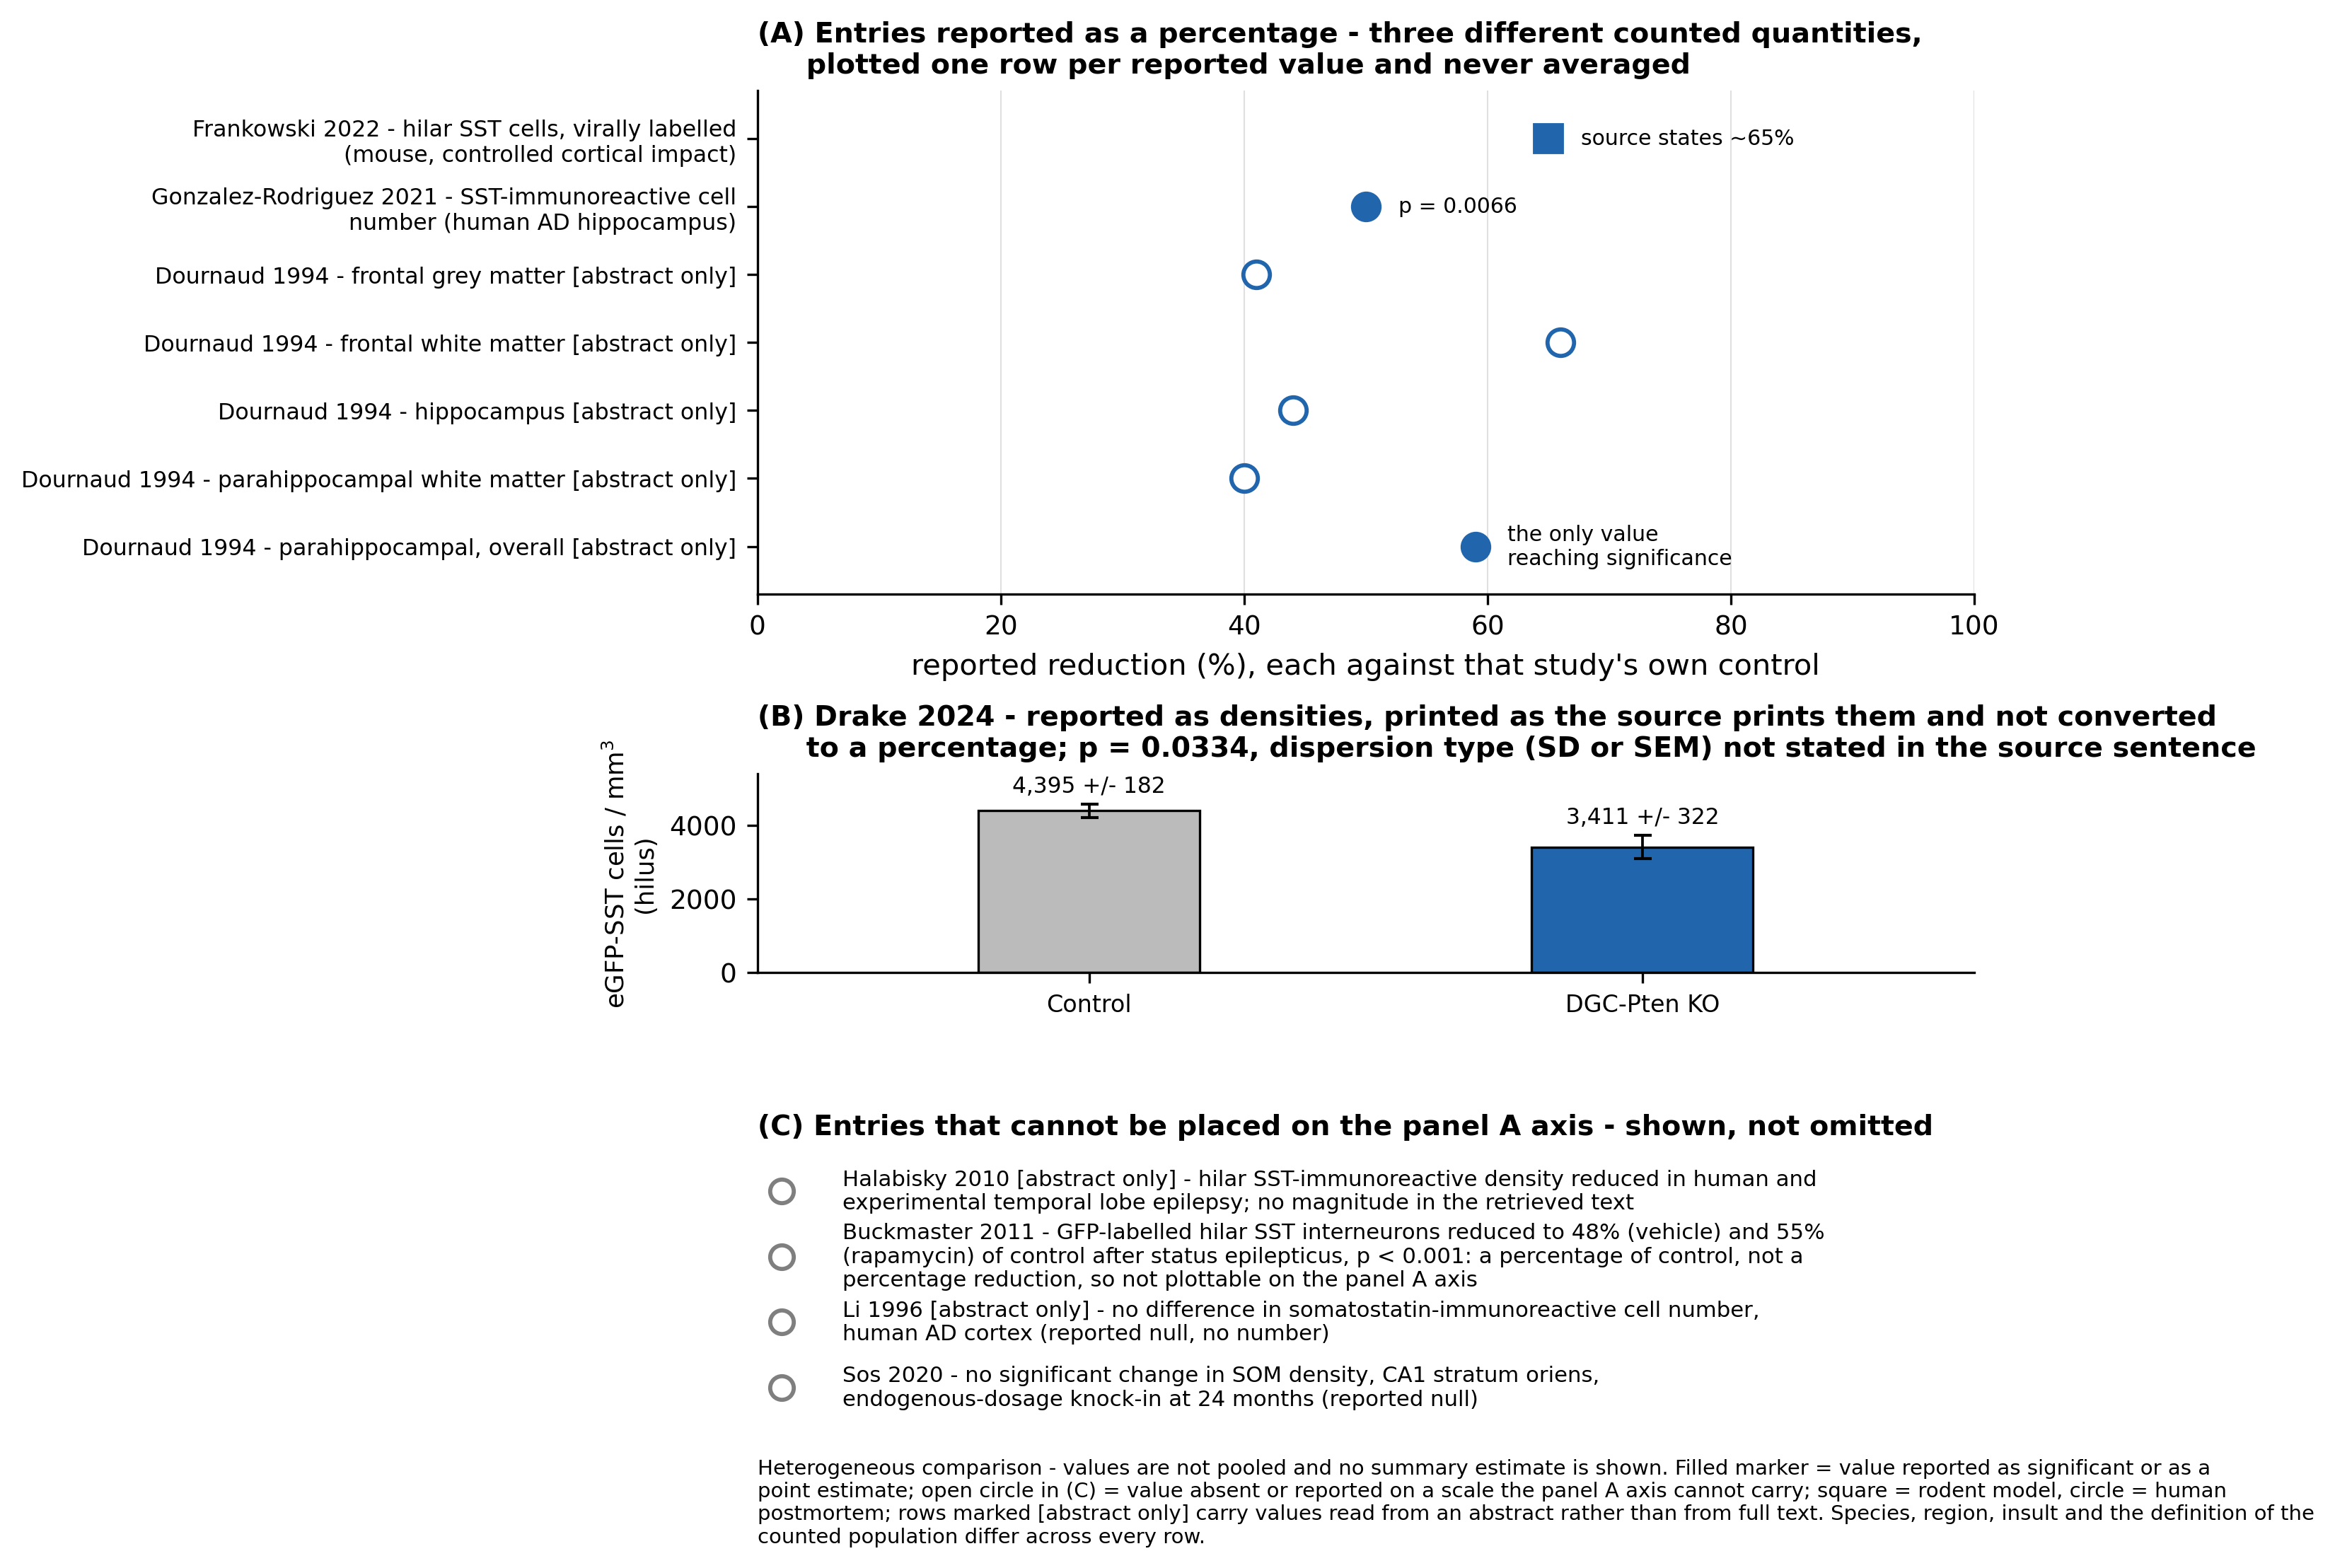
\includegraphics[width=\linewidth]{../figures/fig_sec1_sst_loss_landscape.png}
\caption{\textbf{The same headline, five incompatible measurements.} Reported change in the somatostatin signal across insult and disease, grouped by the unit in which each source reports it; values are not pooled and panels do not share an axis. (A) Entries reported as a percentage reduction: loss of virally labelled hilar SST cells after controlled cortical impact, given in the source as approximately 65\% \citep{Frankowski2022}; a 50\% reduction in SST-immunoreactive cell number in AD hippocampus, p = 0.0066 \citep{GonzalezRodriguez2021}; and five rows from one in-situ-hybridisation series measuring the density of cells containing somatostatin messenger RNA in AD: four regional values (frontal grey matter $-$41\%, frontal white matter $-$66\%, hippocampus $-$44\%, parahippocampal white matter $-$40\%) and, separately, the overall parahippocampal reduction of $-$59\%, the only one of these densities to reach significance \citep{Dournaud1994}. (B) Entries reported as cell densities, printed as the source prints them and not converted to a percentage: hilar eGFP-SST density in a \emph{Pten} knockout model, 4,395 $\pm$ 182 against 3,411 $\pm$ 322 cells/mm$^{3}$, p = 0.0334, dispersion type not stated in the source sentence \citep{Drake2024}. (C) Entries that cannot be placed on the panel A axis, drawn as annotated markers rather than omitted, because omitting them biases the visible distribution towards loss: reduced hilar density in human and experimental temporal lobe epilepsy with no magnitude in the retrieved text \citep{Halabisky2010}; GFP-labelled hilar SST interneurons reduced to 48\% (vehicle) and 55\% (rapamycin) of control after status epilepticus, p < 0.001 --- a percentage of control rather than a percentage reduction, so not plottable on the panel A axis \citep{Buckmaster2011}; and two nulls, no difference in somatostatin-immunoreactive cell number in AD cortex \citep{Li1996b} and no significant change in SOM density in CA1 stratum oriens of an endogenous-dosage knock-in at 24 months \citep{Sos2020}. Heterogeneous comparison --- values are not pooled. Species (mouse, rat, human), region (hilus, CA1, whole hippocampus, neocortex), insult and the definition of the counted population differ across every row; two entries count a reporter-defined subset rather than the whole population, and one counts transcript-labelled cells, which confounds cell loss with transcript downregulation.}
\label{fig-sec1-sst-loss-landscape}
\end{figure}

\subsection{The question, and the shape of the answer}
\label{sec-01-question}

The question this review asks is whether loss or dysfunction of SST interneurons is a shared, causally important feature across neurodegenerative disease; if it is, which mechanisms --- cell-intrinsic fragility, peptide and somatostatin receptor (SSTR1--SSTR5) signalling, or circuit dysregulation --- drive it; how robust the human and model evidence is; and whether any of it justifies SST-targeted biomarkers and therapies. Answering it requires separating the reproducible observation from the inference habitually fused to it, and that separation organises what follows.

\ref{sec-sst-identity} establishes what the SST label spans and what the genetic toolbox actually reports, and \ref{sec-selective-vulnerability} asks what happens to that aggregate under ageing and insult, finding region- and insult-specificity where the field often reads class-intrinsic fragility. The four disease sections then test the same claim in four literatures: \ref{sec-alzheimers}, where the deficit is most reproducible and the proposed amyloid-clearance mechanism is directly disputed; \ref{sec-parkinsons-lewy-body}, where the cortical deficit appears conditional on Alzheimer-type co-pathology; \ref{sec-huntingtons}, where a textbook claim of sparing rests on peptide concentrations measured in atrophic tissue; and \ref{sec-als-ftd}, where cortical inhibition is well measured in patients while this cell class is barely measured in human tissue at all. \ref{sec-circuit-consequences} changes the level of description and shows why a fall in somatostatin signalling degrades dendritic gating and oscillations whether or not a neuron dies; \ref{sec-human-evidence} assembles the human measurements, which carry both the strongest and the weakest claims here; \ref{sec-therapeutics} treats intervention as the direct test of the causal reading; \ref{sec-conflicts-limitations} sorts the accumulated disagreements; and \ref{sec-conclusion} states the conditional answer and the experiments that would change it.

\subsection{What this review can and cannot settle}
\label{sec-01-evidence-base}

Four axes recur across all four disease literatures, and they are named here so that the reader can watch them arrive: what was measured (peptide, transcript, immunoreactive soma, genetically labelled soma, transcriptomically defined nucleus), where, in which model construct, and in which cohort. They are enough to flip the sign of a result. Somatostatin concentrations are elevated rather than reduced in Huntington's disease basal ganglia (caudate 247 $\pm$ 24 against 85 $\pm$ 11 ng/gm) \citep{Aronin1983} while somatostatin-positive density is decreased in the Parkinson's disease amygdala \citep{FloresCuadrado2017} --- peptide assay against cell counting, so part of the cross-disease reversal is a reversal of method. Within amyloid models, SOM interneuron calcium event rates are elevated above wild type, with hyperactivity greatest near plaques \citep{Algamal2022b}, dystrophic SST neurons make up more than 40\% of the hippocampal SST population of a tau--amyloid rat at 15 months \citep{Morrone2022}, and cholinergic drive onto O-LM interneurons falls without any missing cell being counted \citep{Schmid2016} --- functional hyperactivity, structural dystrophy, synaptic weakening and preserved number, reported for the same class in different constructs. Candidate cell-intrinsic causes --- endoplasmic-reticulum stress generated by processing of the somatostatin precursor \citep{Tomoda2022} --- have been reported outside amyloid pathology in a single uncorroborated study with n = 4 per group; the trisomic literature is itself split, with dendritic inhibition involving Martinotti cells reported strengthened in one single-laboratory study and SST-evoked inhibition of granule cells reported age-dependently reduced in another \citep{ZorrillaDeSanMartin2020,Gutmann2026}; and the one account that assigns SST interneurons the leading mechanistic role in an ALS model rests on a single mouse study \citep{Zhang2016}.

This review assembles 726 primary and secondary reports and the disagreements between them, but it is not a census of the field. Retrieval was dominated by one bibliographic database and did not chase citations forward or backward, so every statement that an experiment was not found is a statement about these searches rather than about the literature as a whole. Full text was obtained for the records behind each topic area unevenly --- all 77 records behind the circuit literature, 22 of the 87 behind the human postmortem and fluid evidence --- with the shortfall concentrated in closed-access radioimmunoassay and cerebrospinal fluid work published before 2000, which is why the human synthesis in \ref{sec-human-evidence} rests on the modern open-access cohorts and treats the historical series as an abstract-level record. Searches for disconfirming results were capped, so reported nulls are a top-relevance sample rather than an exhaustive one. \ref{fig-sec1-evidence-base-and-argument-arc} shows where the evidence is thick and where it is thin before any claim is made. Several of the disagreements catalogued in \ref{sec-conflicts-limitations} are left open at the end of this review, and the conclusion in \ref{sec-conclusion} is correspondingly conditional.

\begin{figure}[H]
\centering
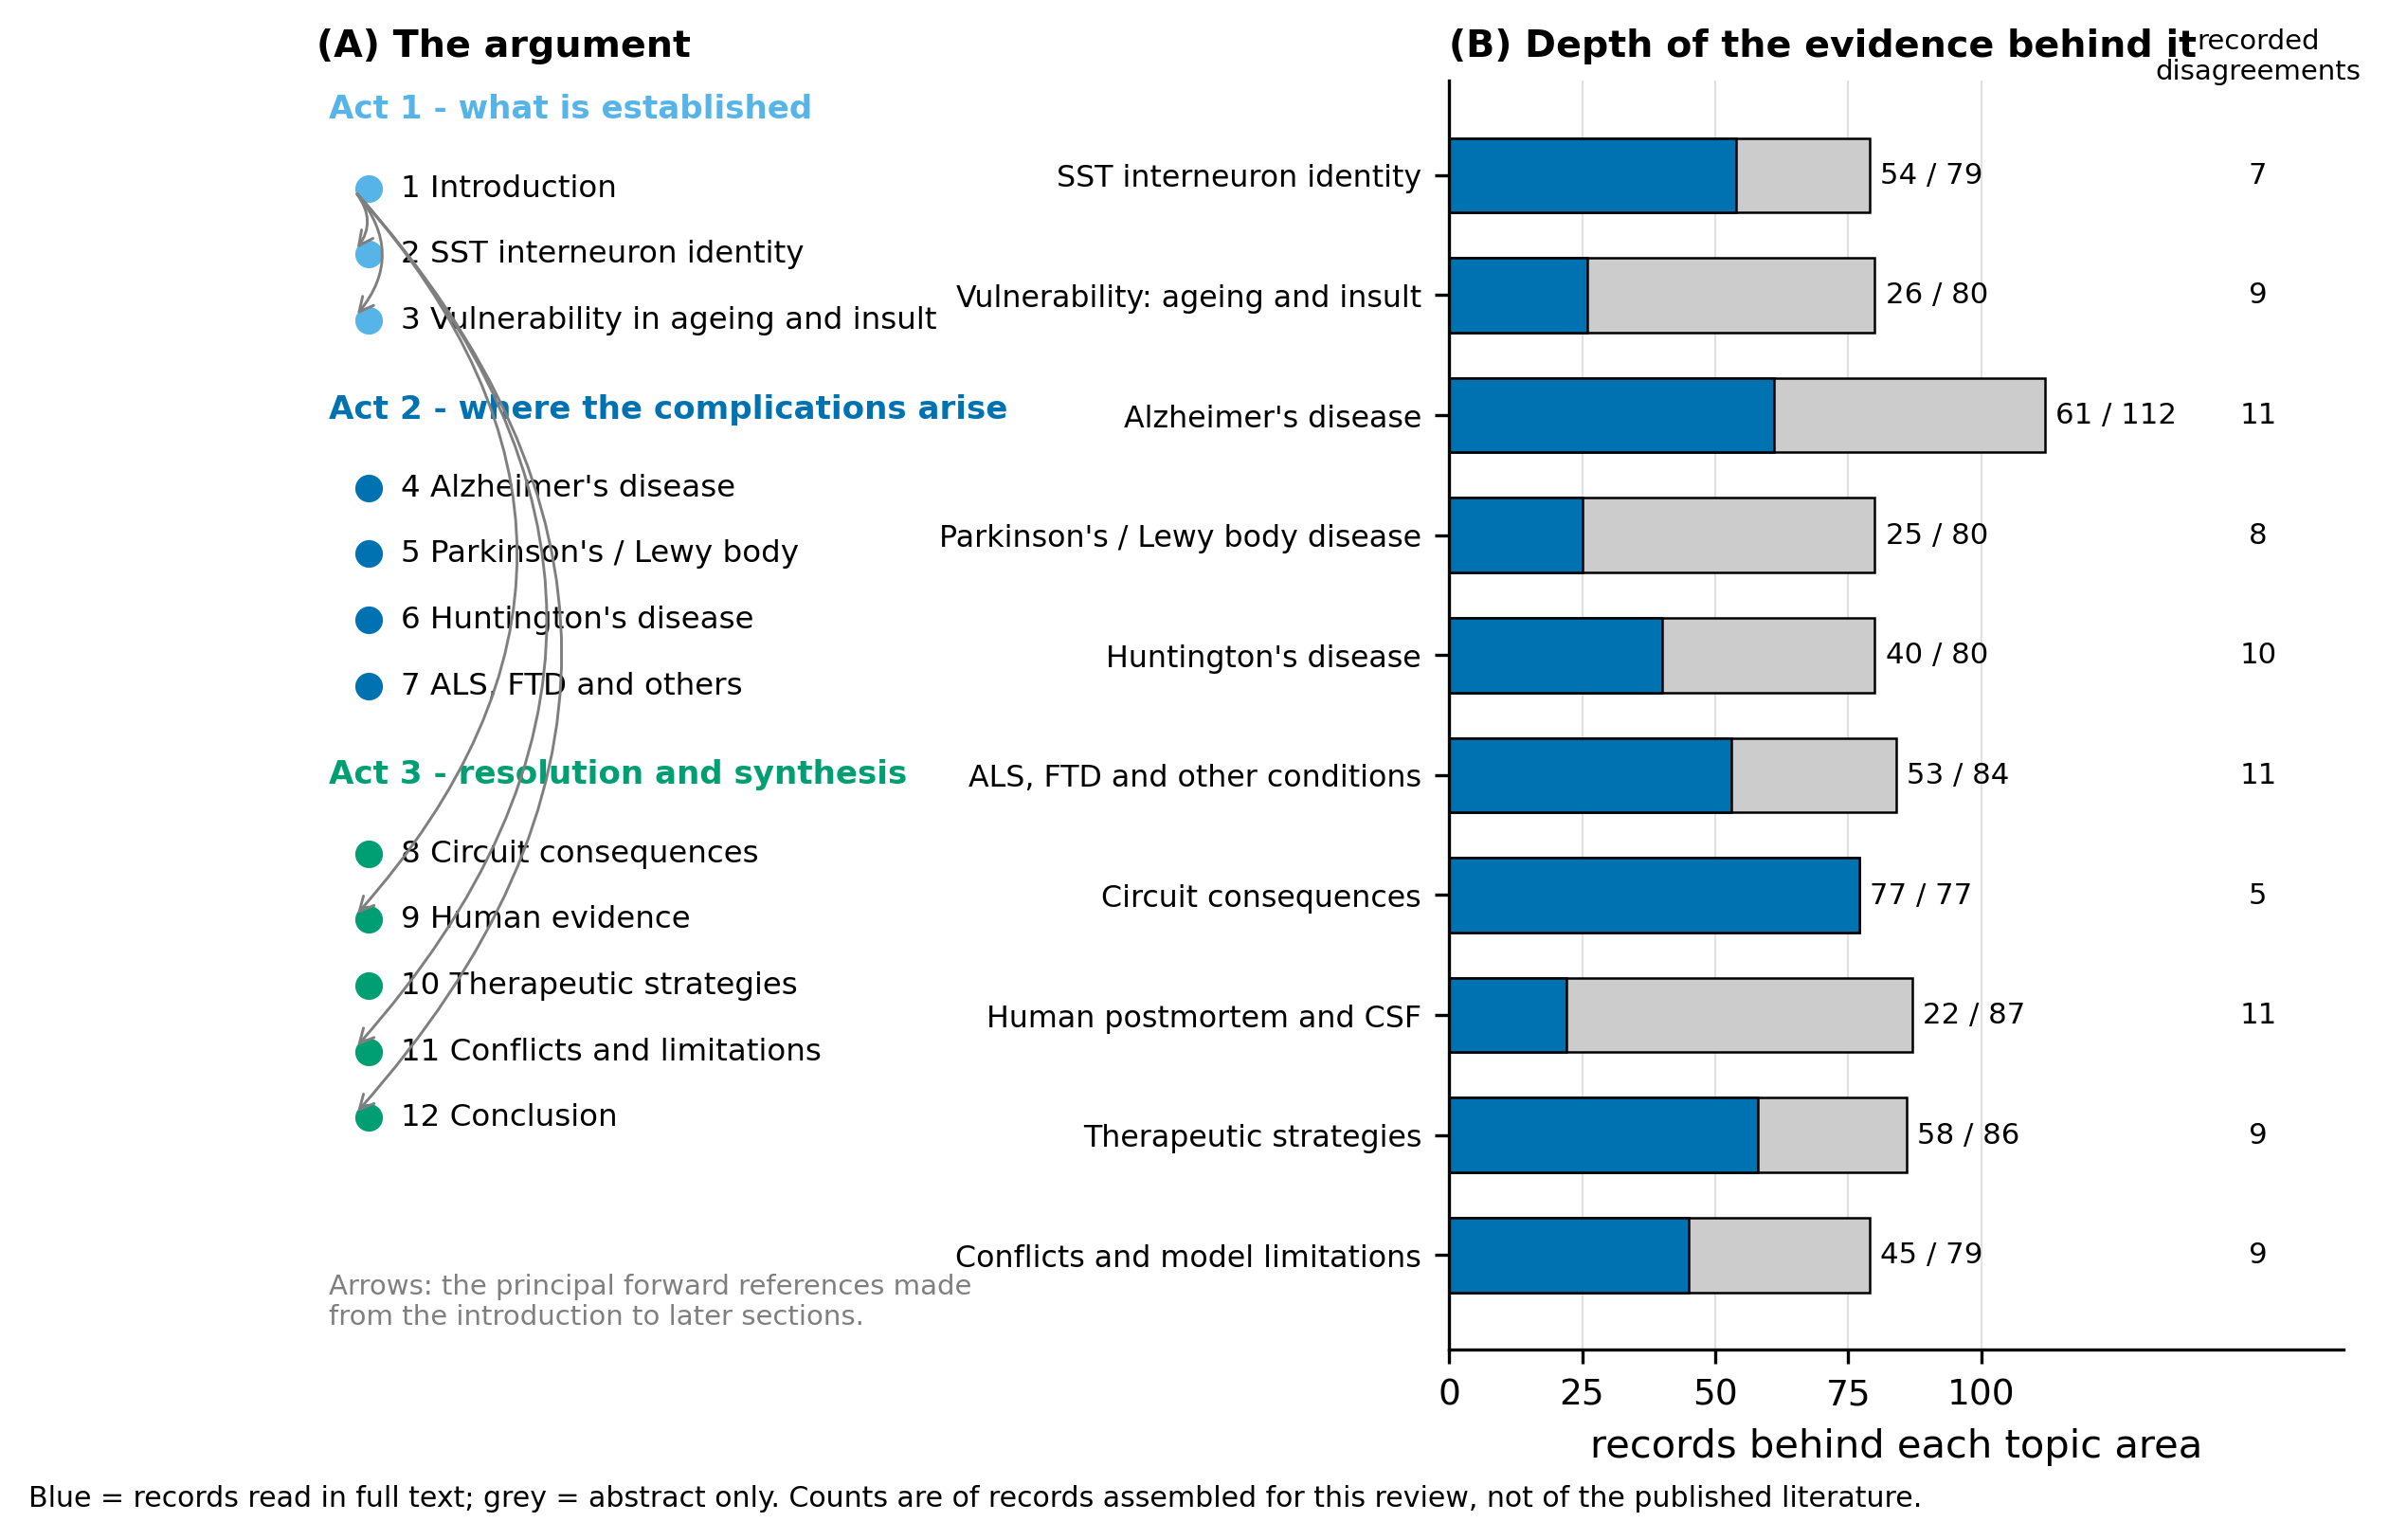
\includegraphics[width=\linewidth]{../figures/fig_sec1_evidence_base_and_argument_arc.png}
\caption{\textbf{The argument, and the depth of the evidence behind each part of it.} (A) The three movements of the review and the sections that carry them, with the principal forward references drawn as edges. (B) For each topic area, the number of records read in full text against the total number of records behind that area, with the number of recorded cross-study disagreements printed at the right. Grey is the abstract-only share. The human postmortem and fluid literature has the lowest full-text coverage (22 of 87) and the circuit literature the highest (77 of 77); the shortfall is concentrated in closed-access work published before 2000, which bears directly on how firmly the oldest radioimmunoassay series can be read. Counts are of records assembled for this review, not of the published literature.}
\label{fig-sec1-evidence-base-and-argument-arc}
\end{figure}

Nothing in what follows reverses the direction of the Alzheimer cortical finding, although \ref{sec-human-evidence} records cortical counting studies that report no difference at all. The argument is about what that fall is a measurement of, and the first requirement is to fix what an SST interneuron is and what the somatostatin signal reports --- the task of \ref{sec-sst-identity}.

\section{SST Interneuron Identity: Transcriptomic Subtypes, Connectivity, and Somatostatin Receptor Signaling}
\label{sec-sst-identity}

The disease literature measures somatostatin and infers a neuron. What that inference buys depends on what the label covers, and the identity literature answers that it covers a great deal: a dozen or more transcriptomic and morpho-electric types with different laminar positions, different postsynaptic partners and different behavioural-state modulation, accessed through driver lines that are not exclusive to it. Four conventions are fixed here and used throughout the review. \emph{Martinotti cell} denotes an axonal-projection phenotype --- an SST cell whose axon ascends to layer 1 --- and not a synonym for SST, because the two criteria in use --- reconstructed axonal morphology and retrograde labelling from layer 1 --- are different operational definitions that have not been applied to the same cells \citep{Jiang2015,Hostetler2023}. Receptor names are standardised to SSTR1--SSTR5, although the primary sources do not share one convention: IUPHAR guidance reserves sst1--5 for recombinant receptors without defined functional characteristics and SST1--5 for fully characterised ones, and explicitly discourages the SSTR form adopted here \citep{Gunther2018}, while other primary sources write Sst1--5 \citep{Lin2013}. Where a source scored its cells by somatostatin immunoreactivity and labelled them SOM-positive, that label is kept when its values are reported and denotes the same measurement as SST-immunoreactive. And \emph{the somatostatin signal} is used only where a cited measurement cannot separate peptide content, transcript level and cell number; that ambiguity is the explicit subject of \ref{sec-selective-vulnerability}. The companion markers that recur throughout are abbreviated PV (parvalbumin), VIP (vasoactive intestinal peptide) and NPY (neuropeptide Y).

\subsection{From one marker to a dozen types}
\label{sec-02-taxonomy}

Three large surveys each resolved roughly a dozen SST groups, and the near-coincidence of their counts is an artefact of three incommensurable counting schemes rather than agreement. \citet{Gouwens2020} identified 13 Sst met-types in mouse visual cortex by integrating Patch-seq morphology, intrinsic physiology and transcriptome in the same cells, substantially more than earlier morphological or electrophysiological schemes had described. \citet{Yao2021} divided the Sst subclass into 11 supertypes across the entire mouse isocortex and hippocampal formation while keeping \emph{Sst Chodl}, the long-range projecting group, as a separate entity outside that count. \citet{Hodge2019} reported 11 SST types that were spatially restricted in human middle temporal gyrus, including distinctive deep-layer \emph{SST TH} and \emph{SST NPY} types. Met-types, supertypes and transcriptomic clusters are three levels of three taxonomies and are not interconvertible: the counts differ in hierarchy level, species and region surveyed, and cannot be ordered by any of those dimensions, as \ref{fig-sec2-sst-taxonomy-and-subtype-fractions} sets out side by side. What anchors the taxonomy to cells are the correspondences: \emph{Sst Chodl} maps onto the Nos1-positive long-range projecting population \citep{Tasic2018}, an upper-layer Calb2-expressing type corresponds to the Calb2-positive Martinotti cells labelled in GIN mice \citep{Tasic2016}, Sst neurons in motor cortex Patch-seq are separated electrophysiologically by large hyperpolarisation sag and rebound \citep{Scala2020}, and 7 of 11 embryonic medial ganglionic eminence (MGE) SST identities match one-to-one with adult types --- four Martinotti, two non-Martinotti and one long-range projecting --- with the programmes reported as conserved between mouse and human \citep{Shi2021}. Human SST subtype data in this literature are sparser than mouse, and that cross-species claim rests on developmental transcriptional programmes rather than on matched adult morpho-electric types. Intersectional genetic targeting of the breadth of the class finds that each subtype occupies a stereotyped laminar position and carries a stereotyped axonal projection pattern \citep{Wu2023}, which is the anatomical reason the class is not a functional unit.

The denominator that disease studies implicitly use is less well anchored than its ubiquity suggests. Cre-line co-labelling in mouse V1 placed Sst-Cre cells at 30\% $\pm$ 1.5 of the GAD67-GFP population, against 36\% $\pm$ 0.5 for Pvalb-Cre and 17\% $\pm$ 1 for VIP-Cre \citep{Pfeffer2013}; a review-level compilation of immunohistochemical counts gives approximately 20--30\% of mouse somatosensory cortical GABA neurons as somatostatin-expressing, with 40--50\% parvalbumin-positive and no overlap between the two \citep{Lin2013}, a second compilation reports parvalbumin cells as the most frequent class at 40--50\% of all interneurons \citep{Williams2021}, and the parvalbumin, SST and 5HT3aR groups together account for nearly all GABAergic neurons of somatosensory cortex \citep{Rudy2010}. Of the three SST-share values, only the Cre-line count is a primary measurement; the other two are literature syntheses, so their agreement is weaker evidence than it looks. Within the class, the Martinotti fraction depends on the criterion applied: about 70\% of recovered SOM-positive neurons in layers 2/3 and 5 of adult V1 were Martinotti cells by axonal reconstruction (133/190) \citep{Jiang2015}, whereas 54 $\pm$ 1\% (N = 17) of all SOM cells across all layers of somatosensory cortex were retrogradely labelled from layer 1 and therefore classified as bona fide Martinotti cells \citep{Hostetler2023}. Layer 5 alone contains approximately 10\% T-shaped Martinotti, 50\% fanning-out Martinotti and 40\% non-Martinotti cells by morphoelectric classification \citep{Nigro2018}, and the older GAD67-GFP lines had already separated these phenotypes, with X98 labelling infragranular calbindin-containing layer-1-targeting cells and X94 labelling stuttering, quasi-fast-spiking cells in and targeting thalamorecipient layers \citep{Ma2006}. Co-marker composition varies by area as well: NPY is co-expressed in about a third of SOM-positive interneurons in cingulate cortex but fewer than 10\% in somatosensory cortex \citep{Riedemann2019}.

\begin{quote}
\noindent\textbf{Evidence conflict: is non-Martinotti identity a property of layer 4 or of cortical area?}\par
Patch-seq mapping of layer 4 interneurons onto transcriptomic SST types sets the earlier view --- that layer-4-targeting SOM-positive cells form a single morphological population, the non-Martinotti cells, whose axons remain in layer 4 rather than ascending to layer 1 --- against its own result: non-fast-spiking SOM-positive neurons in visual cortex layer 4 are predominantly Martinotti cells, in contrast to somatosensory cortex layer 4 where almost all SOM-positive neurons are non-Martinotti, and the two correspond to different transcriptomic types \citep{Scala2019}. Paired recordings across two sensory areas report the same areal split, finding strong morphological differences among layer 4 SST cells, which fell into the non-Martinotti subclass in somatosensory cortex but showed Martinotti-like features in visual cortex \citep{Rachel2025}. The disagreement is between the earlier single-population view, in which non-Martinotti identity belongs to layer 4, and these two studies, in which it belongs to the area; it is open, and it matters because laminar disease findings are routinely generalised across cortex. Quantified morphology and connectivity for non-Martinotti cells outside layer 4 of rodent somatosensory and visual cortex --- in association cortices, hippocampus or human tissue --- was not retrieved by these searches, so the proportions above should not be assumed to transfer.

\end{quote}

\begin{figure}[H]
\centering
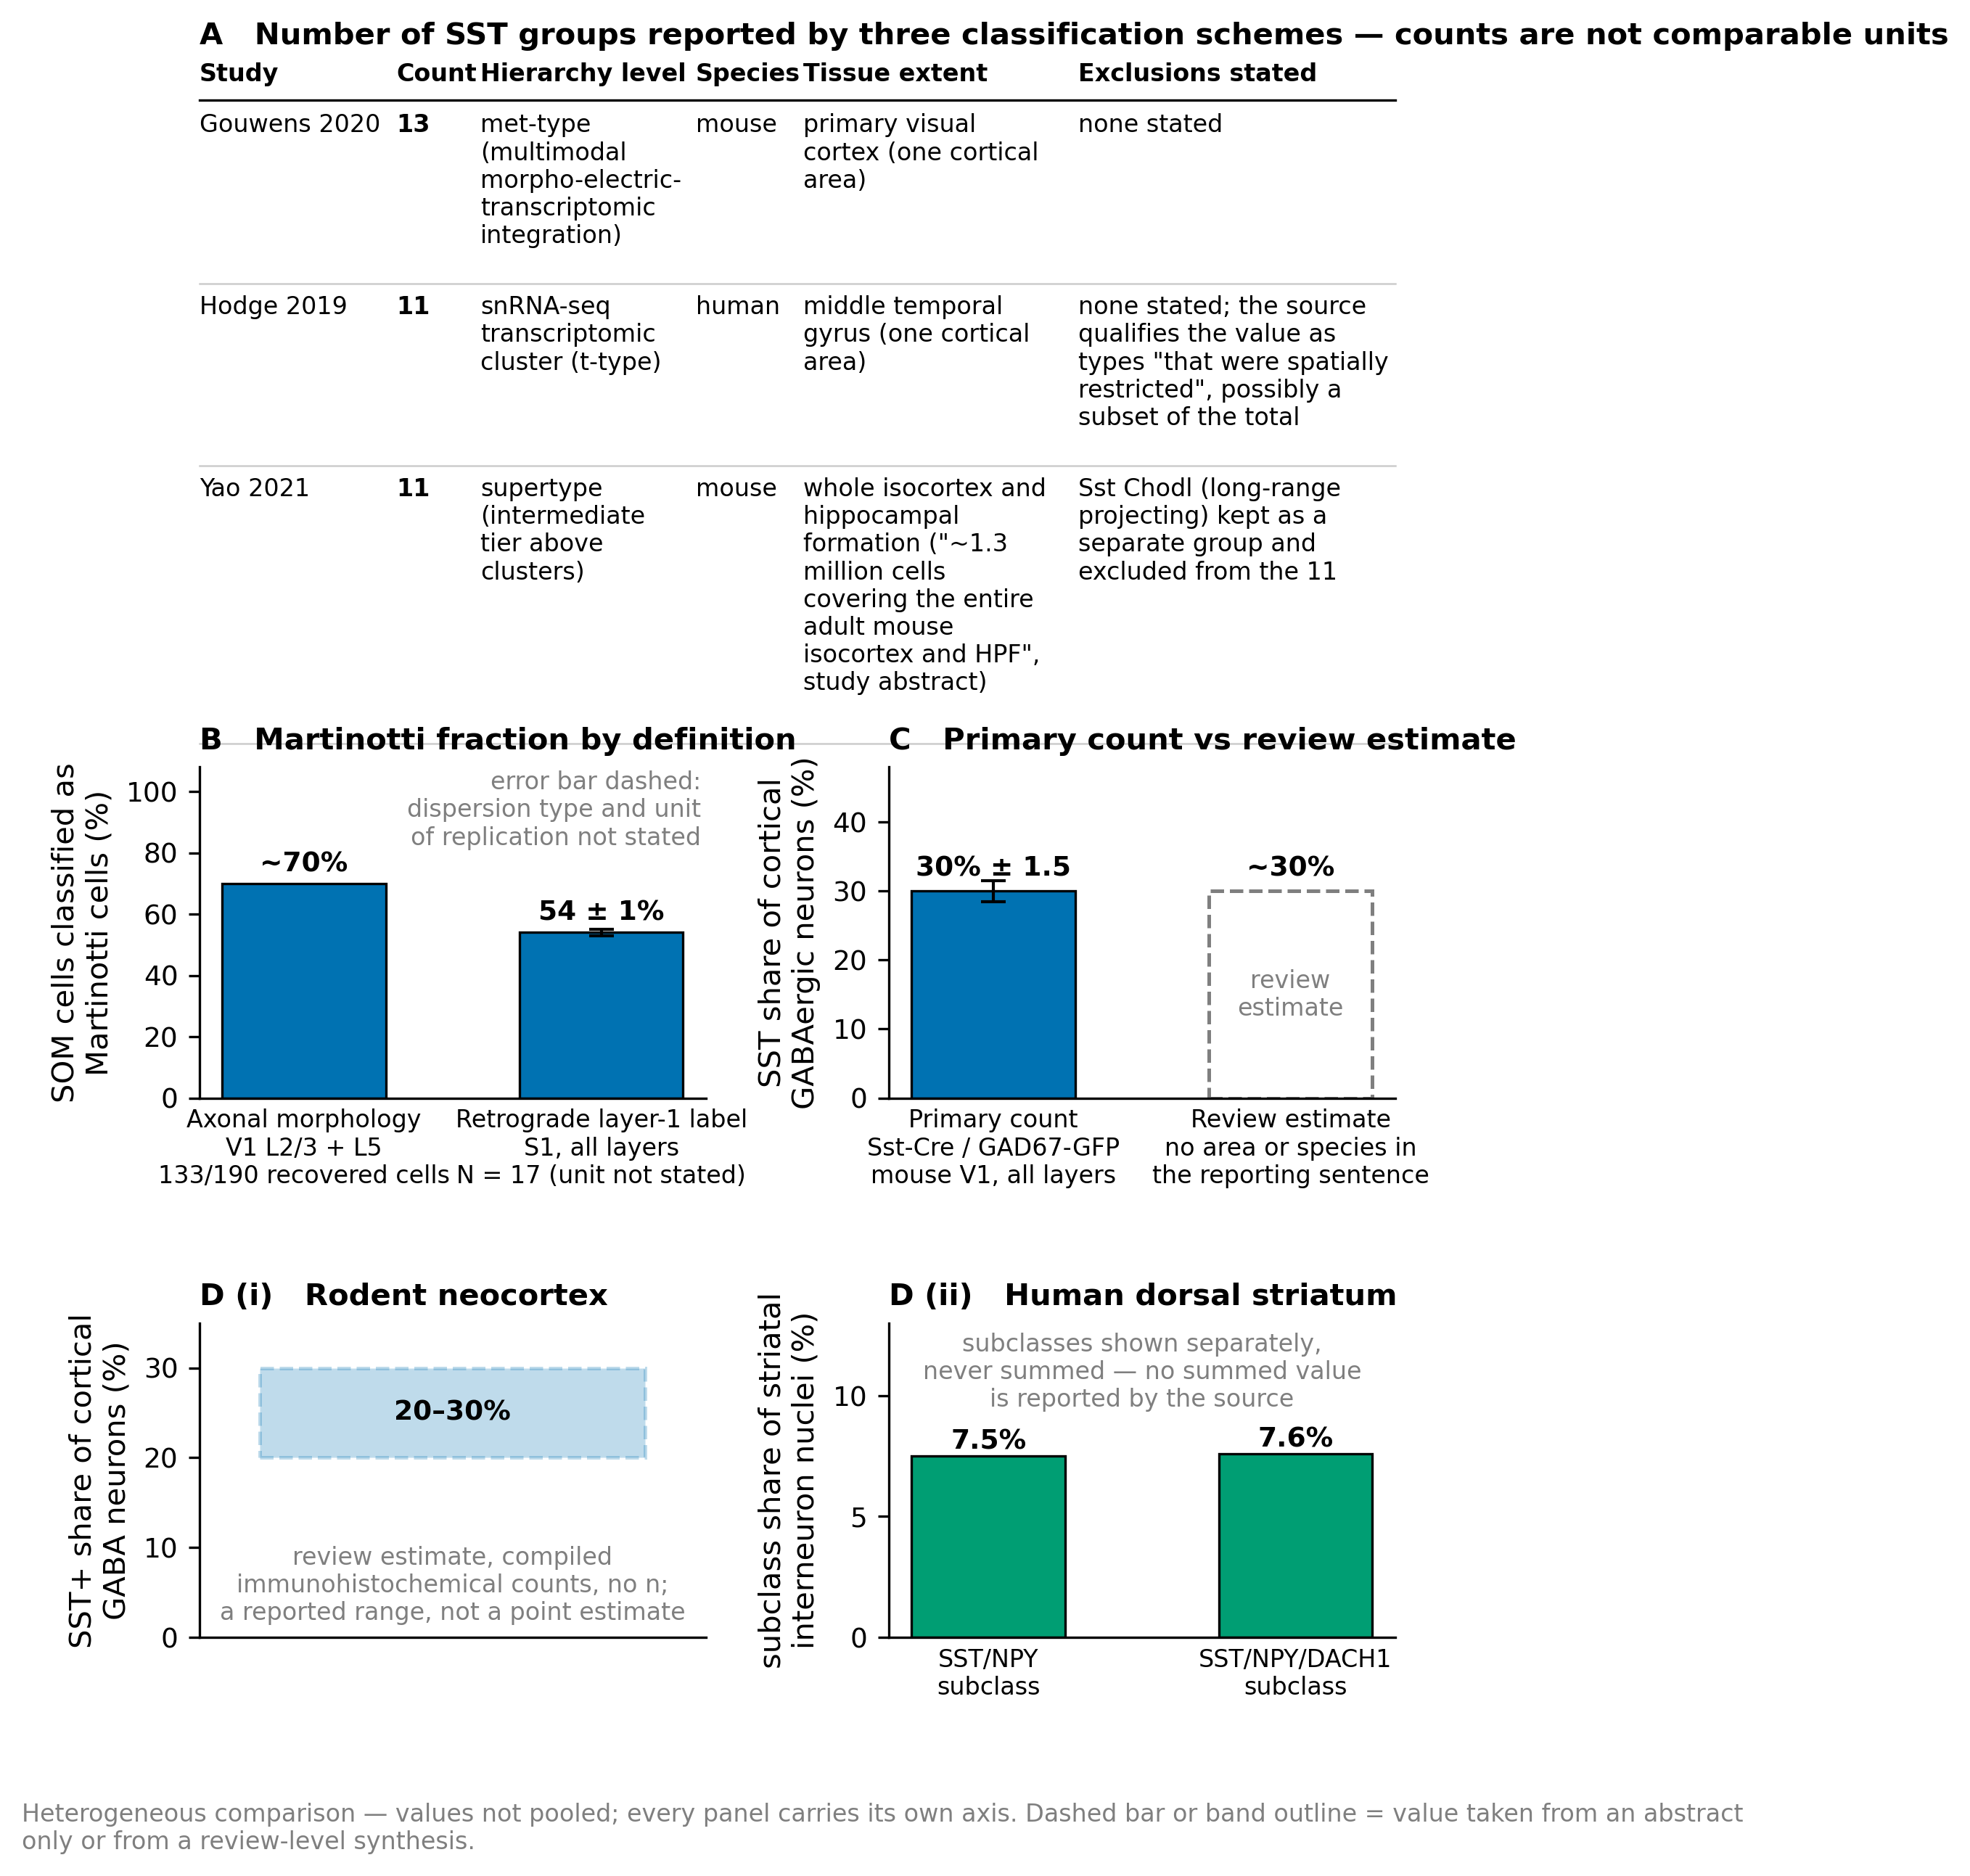
\includegraphics[width=\linewidth]{../figures/fig_sec2_sst_taxonomy_and_subtype_fractions.png}
\caption{\textbf{What the SST label covers.} Four panels, each on its own terms; no value is pooled across panels and no cross-panel difference is annotated. (A) Number of SST groups resolved by three classification schemes, with hierarchy level, species, tissue extent surveyed and stated exclusions given per row \citep{Gouwens2020,Hodge2019,Yao2021}. Counts are not comparable units: met-types (multimodal, mouse V1), snRNA-seq clusters (human MTG) and supertypes (whole mouse isocortex plus hippocampal formation) occupy different levels of three different taxonomies and are not interconvertible. Hodge 2019's 11 is the number of SST types reported as spatially restricted and may not be the total number of SST types in human MTG. Yao 2021's 11 supertypes exclude the Sst Chodl (long-range projecting) group; the other two counts carry no stated exclusion. Species and regional coverage differ: one mouse cortical area, one human cortical area, and the entire mouse isocortex plus hippocampal formation. These three counts cannot be ordered by hierarchy level, species or extent surveyed, and this material does not establish how a type count depends on the extent of tissue surveyed. No entry reports a cell-number denominator or any measure of clustering stability. (B) Fraction of SOM cells classified as Martinotti cells under two operational definitions \citep{Jiang2015,Hostetler2023}. Denominators differ: \textasciitilde{}70\% is of SOM+ cells with recovered morphology in V1 layers 2/3 and 5 only (133/190); 54 $\pm$ 1\% is of all SOM cells across all layers of somatosensory cortex, a denominator that includes layer 4, where SOM cells are largely non-Martinotti. Martinotti identity is assigned by reconstructed axonal morphology in one study and by retrograde labelling from layer 1 in the other; these are different operational definitions. The retrograde-labelling value is reported as "54 $\pm$ 1\% (N = 17)"; what N = 17 counts is not stated in the sentence that reports it or in that study's abstract, so the error bar cannot be interpreted and the difference between the two values must not be read as a measured discrepancy. The all-layer denominator lowers the fraction independently of any areal difference, so the direction of the gap is at least partly a layer-sampling artefact. The ">40\% of all SOM cells" accounting reported in the same retrograde-labelling study is a different quantity and is not plotted here. The morphology-based fraction is conditioned on successful morphological recovery, a sampling step biased toward cells with recoverable long axons. (C) SST share of cortical GABAergic neurons from one primary count and one review estimate \citep{Pfeffer2013,Rudy2010}. The \textasciitilde{}30\% value is a review-level literature estimate (synthesis of marker studies, no reported n), not an independent primary measurement; the agreement between the two values must not be read as independent replication. The review estimate is stated for GABAergic neurons with no cortical area or species specified in the sentence that reports it; only the primary measurement is area-specific (mouse V1, all layers). No regional difference between the two values may be asserted. The two values use different labelling bases: Sst-Cre reporter cells against a GAD67-GFP denominator versus immunohistochemical and in situ SST marker counts. Neither entry supplies a cell-count denominator; the $\pm$ 1.5 cannot be read as a standard error over a known number of animals or sections. Whether and how much non-SST labelling Sst-Cre adds is not established by the sources behind this panel, and no value for it is plotted. (D) SST-expressing fractions reported for rodent neocortex and for human dorsal striatum, on separate axes \citep{Lin2013,Garma2024}. The cortical and striatal values have different denominators (all cortical GABAergic neurons, histologically counted and literature-derived, versus human striatal interneuron nuclei after single-nucleus RNA-seq QC) and different species; they are plotted on separate axes and the difference between them is not a measured regional difference in SST abundance. The cortical value is a review-level literature estimate compiled from immunohistochemical counts, drawn as a range rather than a point estimate, with no reported n. The striatal figure is reported as two separate transcriptomic subclasses (7.5\% and 7.6\%); they are shown separately and are not summed, because no summed value is reported by the source and the taxonomy's fourteen subclasses are not established to make these two exhaustive. The cortical panel rests on a single secondary literature estimate and does not constitute replication. Bar and band edges carry source provenance: a dashed outline marks a value taken from an abstract only or from a review-level synthesis.}
\label{fig-sec2-sst-taxonomy-and-subtype-fractions}
\end{figure}

\subsection{Regional variants are different cells, not the same cell elsewhere}
\label{sec-02-regional-variants}

Hippocampal and striatal SST populations are not cortical Martinotti cells under another name, which matters because the cross-regional vulnerability comparison drawn in \ref{sec-huntingtons} is a comparison between different cells. Single-cell profiling of CA1 divides Sst- and Grm1-expressing stratum oriens cells into Npy/Ngf-positive hippocamposeptal clusters and Pnoc/Reln-positive, Npy-negative clusters identified with oriens-lacunosum moleculare (O-LM) cells \citep{Harris2018}; these two families differ in dendritic and synaptic architecture by three-dimensional electron microscopy, with spine synapses systematically smaller than dendritic shaft synapses on both --- 0.123 $\mu$m$^{2}$ against 0.141 $\mu$m$^{2}$ for glutamatergic inputs onto O-LM dendrites \citep{Takacs2024}. Functionally they diverge from the cortical scheme in two ways. First, output compartment: Chrna2-Cre-defined O-LM$\alpha$2 cells inhibit CA1 pyramidal cells chiefly at the distal apical dendrite \citep{Leao2012}, whereas bistratified cells, also somatostatin-positive, innervate small pyramidal dendritic shafts co-aligned with the Schaffer collateral input \citep{Klausberger2003}, and in the dentate gyrus SOM-positive hilar perforant-path-associated (HIPP) cells inhibit parvalbumin basket cells while rarely receiving reciprocal input from them --- a single study for which no replication was retrieved by these searches \citep{Savanthrapadian2014}. Second, projection: somatostatin- and mGluR1$\alpha$-positive stratum oriens neurons project to subiculum, other cortical areas and the medial septum \citep{Jinno2007}, and dentate SOM-positive axon collaterals run along the fimbria to the medial septum and diagonal band \citep{Yuan2017}. Long-range coordination extends beyond the hippocampal formation: voltage imaging indicates that beta-frequency synchronisation between SST interneuron populations in ventral hippocampus and basolateral amygdala tracks anxiety-related behaviour \citep{Jackson2024}.

The striatal population shares the marker and little else. Striatal persistent low-threshold-spiking interneurons are NADPH-diaphorase-positive and were therefore inferred to release nitric oxide \citep{Kawaguchi1993}, and in human dorsal striatum single-nucleus profiling resolves transcriptomically defined nitrergic interneurons, which the rodent physiological literature has not matched cell for cell, as SST/NPY and SST/NPY/DACH1 subclasses accounting for 7.5\% and 7.6\% of striatal interneurons respectively \citep{Garma2024}. Their output is the opposite of the dense cortical motif: individual persistent low-threshold-spiking cells are weakly and sparsely connected while fast-spiking interneurons carry the bulk of feedforward inhibition \citep{Gittis2010}, and paired recordings only rarely elicited inhibitory responses in spiny projection neurons from NPY-expressing persistent low-threshold-spiking cells \citep{IbanezSandoval2011}. Quantitative output connectivity for adult striatal cells of this class beyond those sparse paired recordings, and its correspondence to the modern transcriptomic subclasses, was not retrieved by these searches. Motor-cortical SOM-positive corticostriatal neurons innervate direct-pathway, indirect-pathway and cholinergic striatal neurons at comparable rates (29\%, 22\% and 40\%) \citep{Melzer2017}, so cortex and striatum are also linked by SST-positive long-range axons rather than being independent compartments. A further nitrergic population complicates marker-based reasoning: deep-layer neocortical neurogliaform cells expressing Id2 and Nkx2.1 and weakly immunoreactive for neuronal nitric oxide synthase are selectively active during the non-REM down state \citep{Valero2021}. The striatal SST/NPY/nitrergic class defined here is the population whose sparing is debated in \ref{sec-huntingtons}.

\subsection{Input-output logic: dendritic targeting, disinhibition and recurrence}
\label{sec-02-input-output}

The motif the disease sections need is dendritic inhibition with a gain-control signature, and it is well supported. Optical activation of SOM interneurons significantly reduced calcium signals in 57\% (73/127) of randomly imaged pyramidal spines \citep{Chiu2013}; disynaptic inhibition between layer 5 pyramidal cells is mediated by Martinotti cells \citep{Silberberg2007}; and silencing SOM interneurons in running mice increased the probability of CA1 pyramidal burst firing, from 45\% more spike doublets to 280\% more bursts of five or more spikes \citep{Royer2012}. The lateral footprint of SST-mediated inhibition in V1 is broader than that of parvalbumin-mediated inhibition, which a circuit model, anatomical tracing and subthreshold measurements link to divisive rather than subtractive control of contrast sensitivity \citep{DelRosario2025}, and the Martinotti-to-pyramidal synapse is pharmacologically distinguished by $\alpha$5-containing GABA-A receptors not expressed at the other synapses those cells make \citep{Donato2022}. Output is not uniform across the class, however. Layer 4 SOM interneurons in barrel cortex connected to fast-spiking interneurons far more often than to principal neurons (62\%, 37/60 versus 35\%, 31/89) --- against a reported 100\% connection probability for layer 2/3 Sst cells onto nearby pyramids in V1, a value stated jointly for Pvalb and Sst cells and without a pair denominator \citep{Pfeffer2013} --- and reducing their activity increased layer 4 fast-spiking firing by 32.8\% during up states --- a disinhibitory rather than a dendrite-gating role \citep{Xu2013}. Dense electron-microscopic reconstruction of mouse visual cortex reaches a compatible conclusion without molecular labels: inhibitory neurons show widespread target specificity, and groups with similar subclass-level targeting differ in which postsynaptic compartment they target, an organising principle for inhibitory connectivity that the authors describe as complementary to, but distinct from, cell types \citep{SchneiderMizell2025}. In awake animals the class is also state-dependent, with layer 2/3 SOM neurons of barrel cortex hyperpolarising and reducing firing during both passive and active whisker sensing while nearby cell types are excited \citep{Gentet2012}.

Inputs onto SST cells are the second half of the motif, and here the quantitative picture fragments. Paired recordings in V1 layer 2/3 found VIP cells inhibiting Sst cells with a connection probability of 62.5\%, against only about 12.5\% onto pyramids \citep{Pfeffer2013}; inactivating VIP interneurons during motor cortex input reduced inhibition of SST interneurons by about half in barrel cortex \citep{Lee2013}; and brief activation of the sparse VIP population changed firing rates in about 20\% of cortical cells \citep{Pi2013}. But the hit rate depends on the laminar motif: approximately 40--45\% of tested layer 4 SST cells were inhibited by layer 2/3 VIP cells in both somatosensory and visual cortex \citep{Rachel2025}, whereas intralaminar layer 5 pairs gave 21.1\% (15/71) for VIP-to-SST and a comparable 24.7\% (18/73) for PV-to-SST \citep{Preuss2025}; \ref{fig-sec2-sst-connectivity-motif-disagreements} places each value beside the laminar scope it was measured in. These are different statistics as well as different motifs, and the second study reports its own translaminar rate as similar to its intralaminar one, so the gap is not evidence of a laminar gradient. Connectivity also does not guarantee control: chemogenetic silencing of CA1 VIP interneurons left excitatory input processing in superficial pyramidal cells unchanged at maximal stimulation intensity \citep{Iloun2026}, against that 40--45\% hit rate \citep{Rachel2025} --- a measured synapse is not a measured function. State modulation has been contested in the same way. Locomotion suppressed calcium responses of V1 SST cells in one study \citep{Fu2014} and generally increased their baseline activity in another \citep{Dipoppa2018}; the later work attributes the sign difference to visual condition rather than to the cells, and in-situ-transcriptomic recording resolves the class further still, with \emph{Sst Tac1} cells most active during synchronised states and \emph{Sst Reln} cells more active during running --- a subtype-level dissociation reported once, with no replication retrieved \citep{Bugeon2022}. Additional control layers continue to be added on top of the motif: NDNF-expressing layer 1 interneurons are reported to suppress SOM interneuron output in a layer-specific manner in auditory cortex, also a single report \citep{Naumann2025}, GABA-B receptor activation reduced spontaneous SST interneuron firing by 60\% \citep{Kanigowski2023}, GABAergic synapses onto CA1 SST and PV interneurons differ in integrin-dependent modulation \citep{Brzdak2023}, theta-patterned stimulation of pyramidal axons potentiates excitatory input onto O-LM interneurons to 144 $\pm$ 15\% of control \citep{Sammari2022}, and associative learning produces a durable, target-specific reduction of SST output that depends on stimulus--reward contingency rather than stimulus exposure \citep{Park2025}. These last results are single studies; their direction matters more than their magnitude for now. Dendritic targeting and the VIP--SST--PV motif are the mechanism by which SST dysfunction becomes an oscillatory and mnemonic phenotype in \ref{sec-circuit-consequences}.

\begin{quote}
\noindent\textbf{Evidence conflict: do SST cells inhibit each other?}\par
Paired recordings in mouse V1 reported more similarities than differences between layer 2/3 and layer 5 inhibitory networks, including a comparable \emph{lack} of Sst-to-Sst and Pvalb-to-Sst connections in both \citep{Pfeffer2013}. Large-scale multipatch recordings in mouse and human neocortex explicitly contradict this, observing connections between Sst neurons in every layer \citep{Campagnola2022}. The candidate explanations are measurement scale, detection sensitivity and driver-line specificity rather than biology --- the larger survey probed far more pairs --- though none has been tested directly, and the subtype-resolved confirmation of these connections rests on a small number of probed pairs, a count carried by no quoted sentence from that study, so a subtype-resolved recurrent-connectivity estimate at scale remains unavailable. Functional evidence favours some recurrent inhibition, since the increase in cooperative recruitment among SOM cells was significantly reduced to 16 $\pm$ 7\% under GABA receptor blockade \citep{Karnani2016}. The conflict is unresolved, and it is consequential: whether the class can disinhibit itself changes the predicted network effect of losing part of it.

\end{quote}

\begin{figure}[H]
\centering
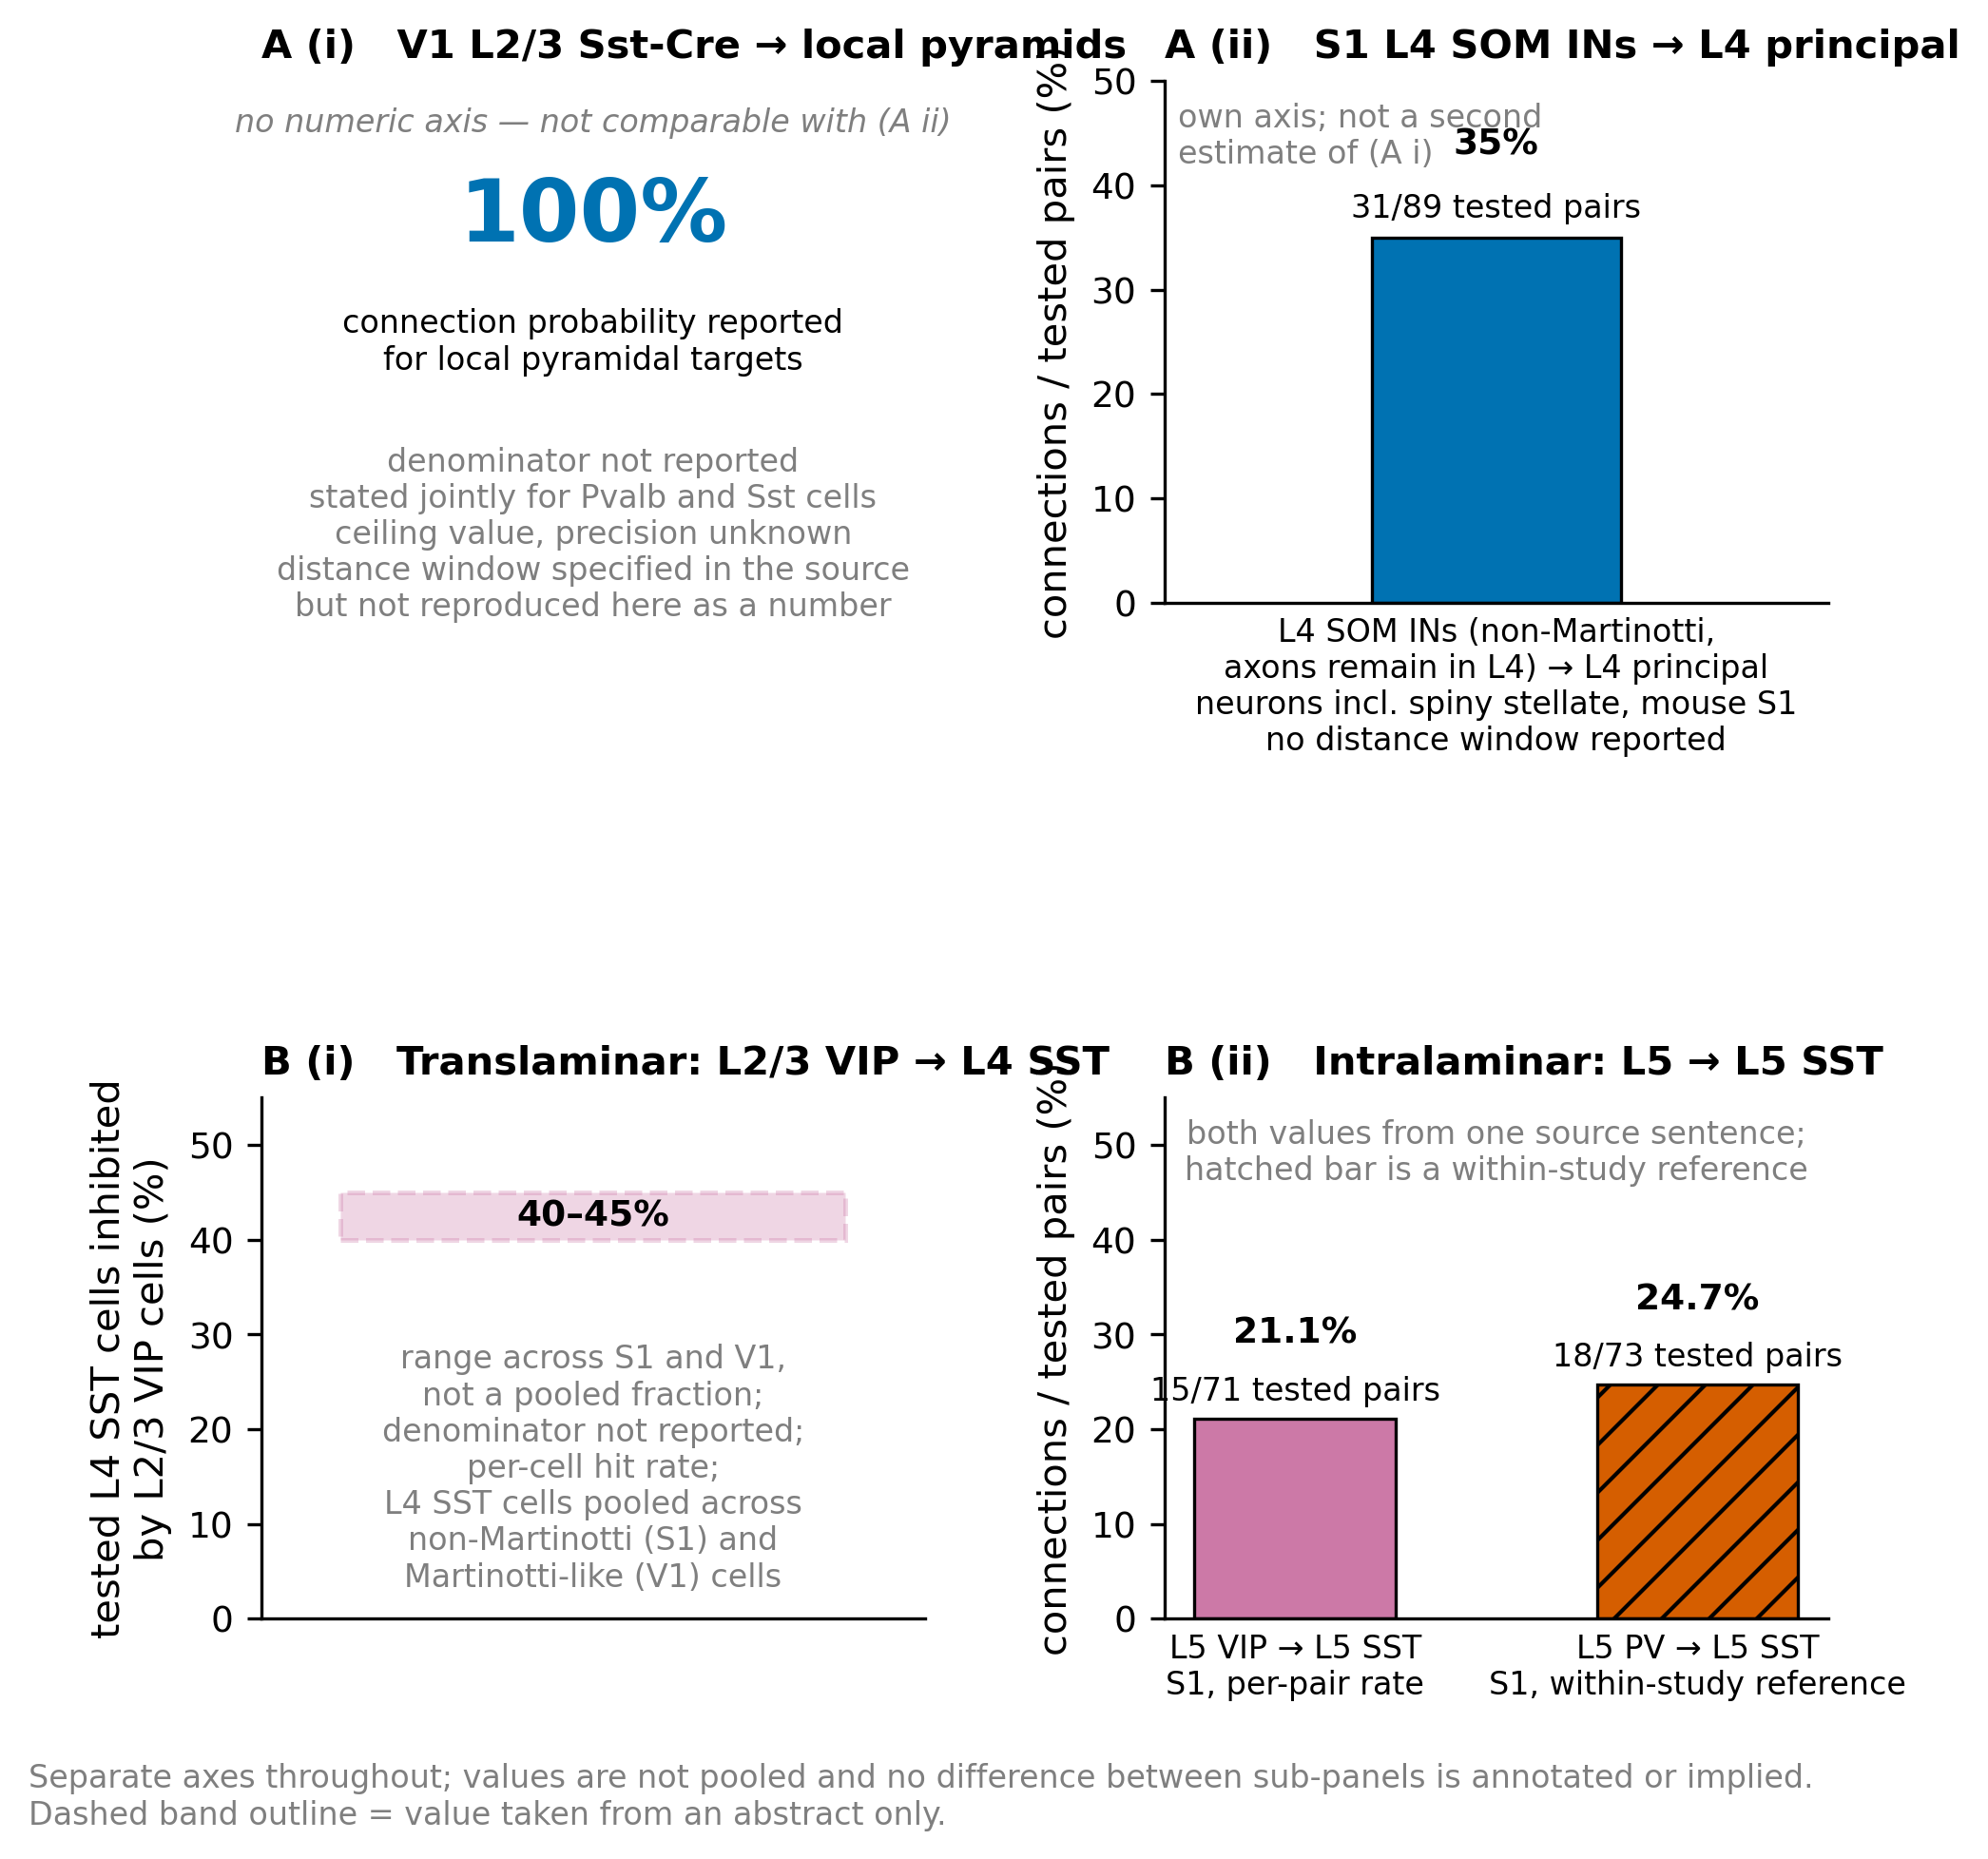
\includegraphics[width=\linewidth]{../figures/fig_sec2_sst_connectivity_motif_disagreements.png}
\caption{\textbf{Connection probabilities with their scope attached.} Each sub-panel carries its own axis; values are never pooled and no difference between sub-panels is annotated or implied. (A) SST output onto local excitatory targets, reported separately for two presynaptic populations \citep{Pfeffer2013,Xu2013}. In the layer 4 source the excitatory target is the minority pathway: layer 4 SOM interneurons there target mainly fast-spiking interneurons, and it is layer 2/3 SOM interneurons in that study that target mainly pyramidal cells. The two values are not two estimates of one connection probability: layer 2/3 Sst cells onto local pyramidal neurons in V1 versus layer 4 SOM interneurons, a predominantly non-Martinotti population whose axons stay within layer 4, onto layer 4 principal neurons in S1. The 100\% value carries no reported pair denominator and is stated in its source jointly for Pvalb and Sst cells; the 35\% value is 31 of 89 tested pairs. The absence of an error bar on the former is not a statement of precision. The inter-somatic distance window is specified for one entry and unreported for the other; connection probability falls steeply with distance, so part of any apparent gap is a sampling-window artefact. Only the SOM-to-principal-neuron value (35\%) is plotted from Xu 2013; that study's SOM-to-fast-spiking-interneuron value is a different postsynaptic population and is not shown. Area and layer differ together (V1 layer 2/3 versus S1 layer 4); the comparison cannot separate areal from laminar effects. The two values are shown on separate axes and are not two values of one measured quantity. (B) Inhibitory input onto SST cells, grouped by laminar motif \citep{Rachel2025,Preuss2025}. The two values are different connectivity motifs: translaminar layer 2/3 VIP onto layer 4 SST cells (reported for both S1 and V1) versus intralaminar layer 5 VIP onto layer 5 SST cells in S1. The 40--45\% figure is a range reported across two cortical areas, not a single pooled fraction, and no tested-pair denominator is given; the 21.1\% figure is 15 of 71 tested pairs. The layer 4 SST cells behind the 40--45\% value are morphologically heterogeneous by the source study's own account (non-Martinotti in S1, Martinotti-like in V1) and are pooled in that single value. The difference between the two values must not be read as a laminar gradient in VIP-to-SST connectivity: the layer 5 study reports that its own translaminar layer 2/3 VIP to layer 5 SST rate is similar to its intralaminar rate. The two values are also different statistics: a per-cell hit rate versus a per-pair connection rate. The layer 5 PV-to-SST value (24.7\%, 18/73) is a within-study reference from the same source sentence, not a cross-study comparator. Dashed edges mark values taken from abstracts only.}
\label{fig-sec2-sst-connectivity-motif-disagreements}
\end{figure}

\subsection{Somatostatin as a transmitter: processing, release and SSTR1-SSTR5 signalling}
\label{sec-02-peptide}

Somatostatin is a diffusible neuromodulator as well as a cell-identity marker, so the peptide deserves treatment as a signal in its own right. All five receptors are described as sharing G$\alpha$i-dependent inhibition of adenylyl cyclase, with SSTR5 additionally engaging protein tyrosine phosphatases, MAPK and cytosolic calcium and potassium signalling --- a review-level account, no primary measurement of the pan-receptor claim having been retrieved here \citep{Gunther2018}; cloned SSTR1 and SSTR2 expressed in Chinese hamster ovary cells bind somatostatin-14 with apparently higher affinity than somatostatin-28 \citep{Yamada1992}; and structure-guided mutagenesis of the SSTR2 ligand-binding pocket shows that disrupting an intramolecular bridge leaves less than 20\% inhibition of cAMP production where wild-type receptor inhibition is complete \citep{Heo2022}. Receptor subtypes are also described as influencing one another when co-expressed in the same cell, with SSTR5 affecting SSTR2 internalisation and trafficking, again at review level rather than from a primary measurement retrieved here \citep{Lin2013}. At the cellular level, both somatostatin-28 and somatostatin-14 elicit a steady outward current in CA1 pyramidal neurons by selectively augmenting the M-current \citep{Moore1988}; pharmacological SSTR activation hyperpolarises layer 2/3 prelimbic pyramidal neurons, recapitulating optogenetic recruitment of SST interneurons \citep{Brockway2023}; and selective SSTR4 agonism augmented the M-current in layer V pyramidal neurons (p = 0.016) but not in interneurons (p = 0.53) or layer II--IV pyramidal neurons (p = 0.56), a cell-type specificity reported by a single study, with no replication retrieved by these searches \citep{Kecskes2020}. Peptidergic and GABAergic output are mechanistically separable, since somatostatin depresses glutamatergic transmission presynaptically while its postsynaptic effects are pronounced in pyramidal cells and little to absent in SST interneurons and layer 1 interneurons \citep{Riedemann2024}. In human cortex the substrate exists: \emph{SST}, \emph{SSTR1} and \emph{SSTR2} are among the most highly expressed interneuron neuropeptide--receptor transcript pairs in prefrontal cortex \citep{Zhong2022}, and a humanised SSTR4 reporter line maps human promoter-driven expression onto defined forebrain populations \citep{Nemes2021}. Receptor-level pharmacology nonetheless remains thin: newly characterised small-molecule SSTR4 agonists showed efficacies and potencies merely comparable to the established reference compound \citep{Biskup2026}, and in \emph{Sstr2}-null mice intrahippocampal kainate produced a 52\% reduction in EEG ictal activity relative to wild-type littermates, a single result now more than two decades old for which no replication was retrieved \citep{Moneta2002}. The receptor pharmacology summarised here is the target rationale examined in \ref{sec-therapeutics}, and the peptide-processing account feeds the somatostatin--neprilysin--amyloid axis in \ref{sec-alzheimers}.

Three load-bearing links in that account are, however, not established by the retrieved literature, and \ref{fig-sec2-sst-peptide-and-sstr-signalling} draws them as such. No primary study directly measuring prosomatostatin processing into somatostatin-14 and somatostatin-28, or activity-dependent peptide release from identified cortical or hippocampal SST interneurons, was retrieved by these searches; what exists is an assay for inducing and inhibiting somatostatin release from prefrontal slices under optogenetic stimulation \citep{Dao2019}, light-triggered release of somatostatin-14 from implanted nanovesicles read out by near-infrared receptor-based sensing, which showed reduced but synchronised transmission within 130 $\mu$m and markedly smaller, delayed transmission at longer distances \citep{Xiong2022}, direct nanosampling of extracellular fluid detecting somatostatin among the prominent cortical prohormone-derived peptides, in a preparation whose neuropeptide concentrations lie in the nanomolar-to-picomolar range \citep{Li2025}, and genetically encoded sensors able to detect peptide binding at nanomolar concentrations \citep{Wang2023b}. All four are exogenous release, bulk stimulation or detection-capability results rather than measurements of endogenous release during behaviour, so the dose and spatial range of physiological somatostatin signalling remain unestablished. Second, no transcriptomic or immunohistochemical study mapping SSTR1--SSTR5 onto identified postsynaptic cell types --- pyramidal versus PV versus VIP --- was retrieved, which is a gap directly beneath every subtype-selective therapeutic proposal. Third, the co-release of somatostatin with GABA from the same terminals is widely repeated and appears here only as a review-level assertion \citep{Gunther2018}; the primary demonstration at identified synapses, with separable time courses, was not retrieved, and whether the peptide and the transmitter are co-packaged determines whether peptidergic signalling tracks fast inhibition or operates as an independent, activity-threshold-gated channel.

\begin{figure}[H]
\centering
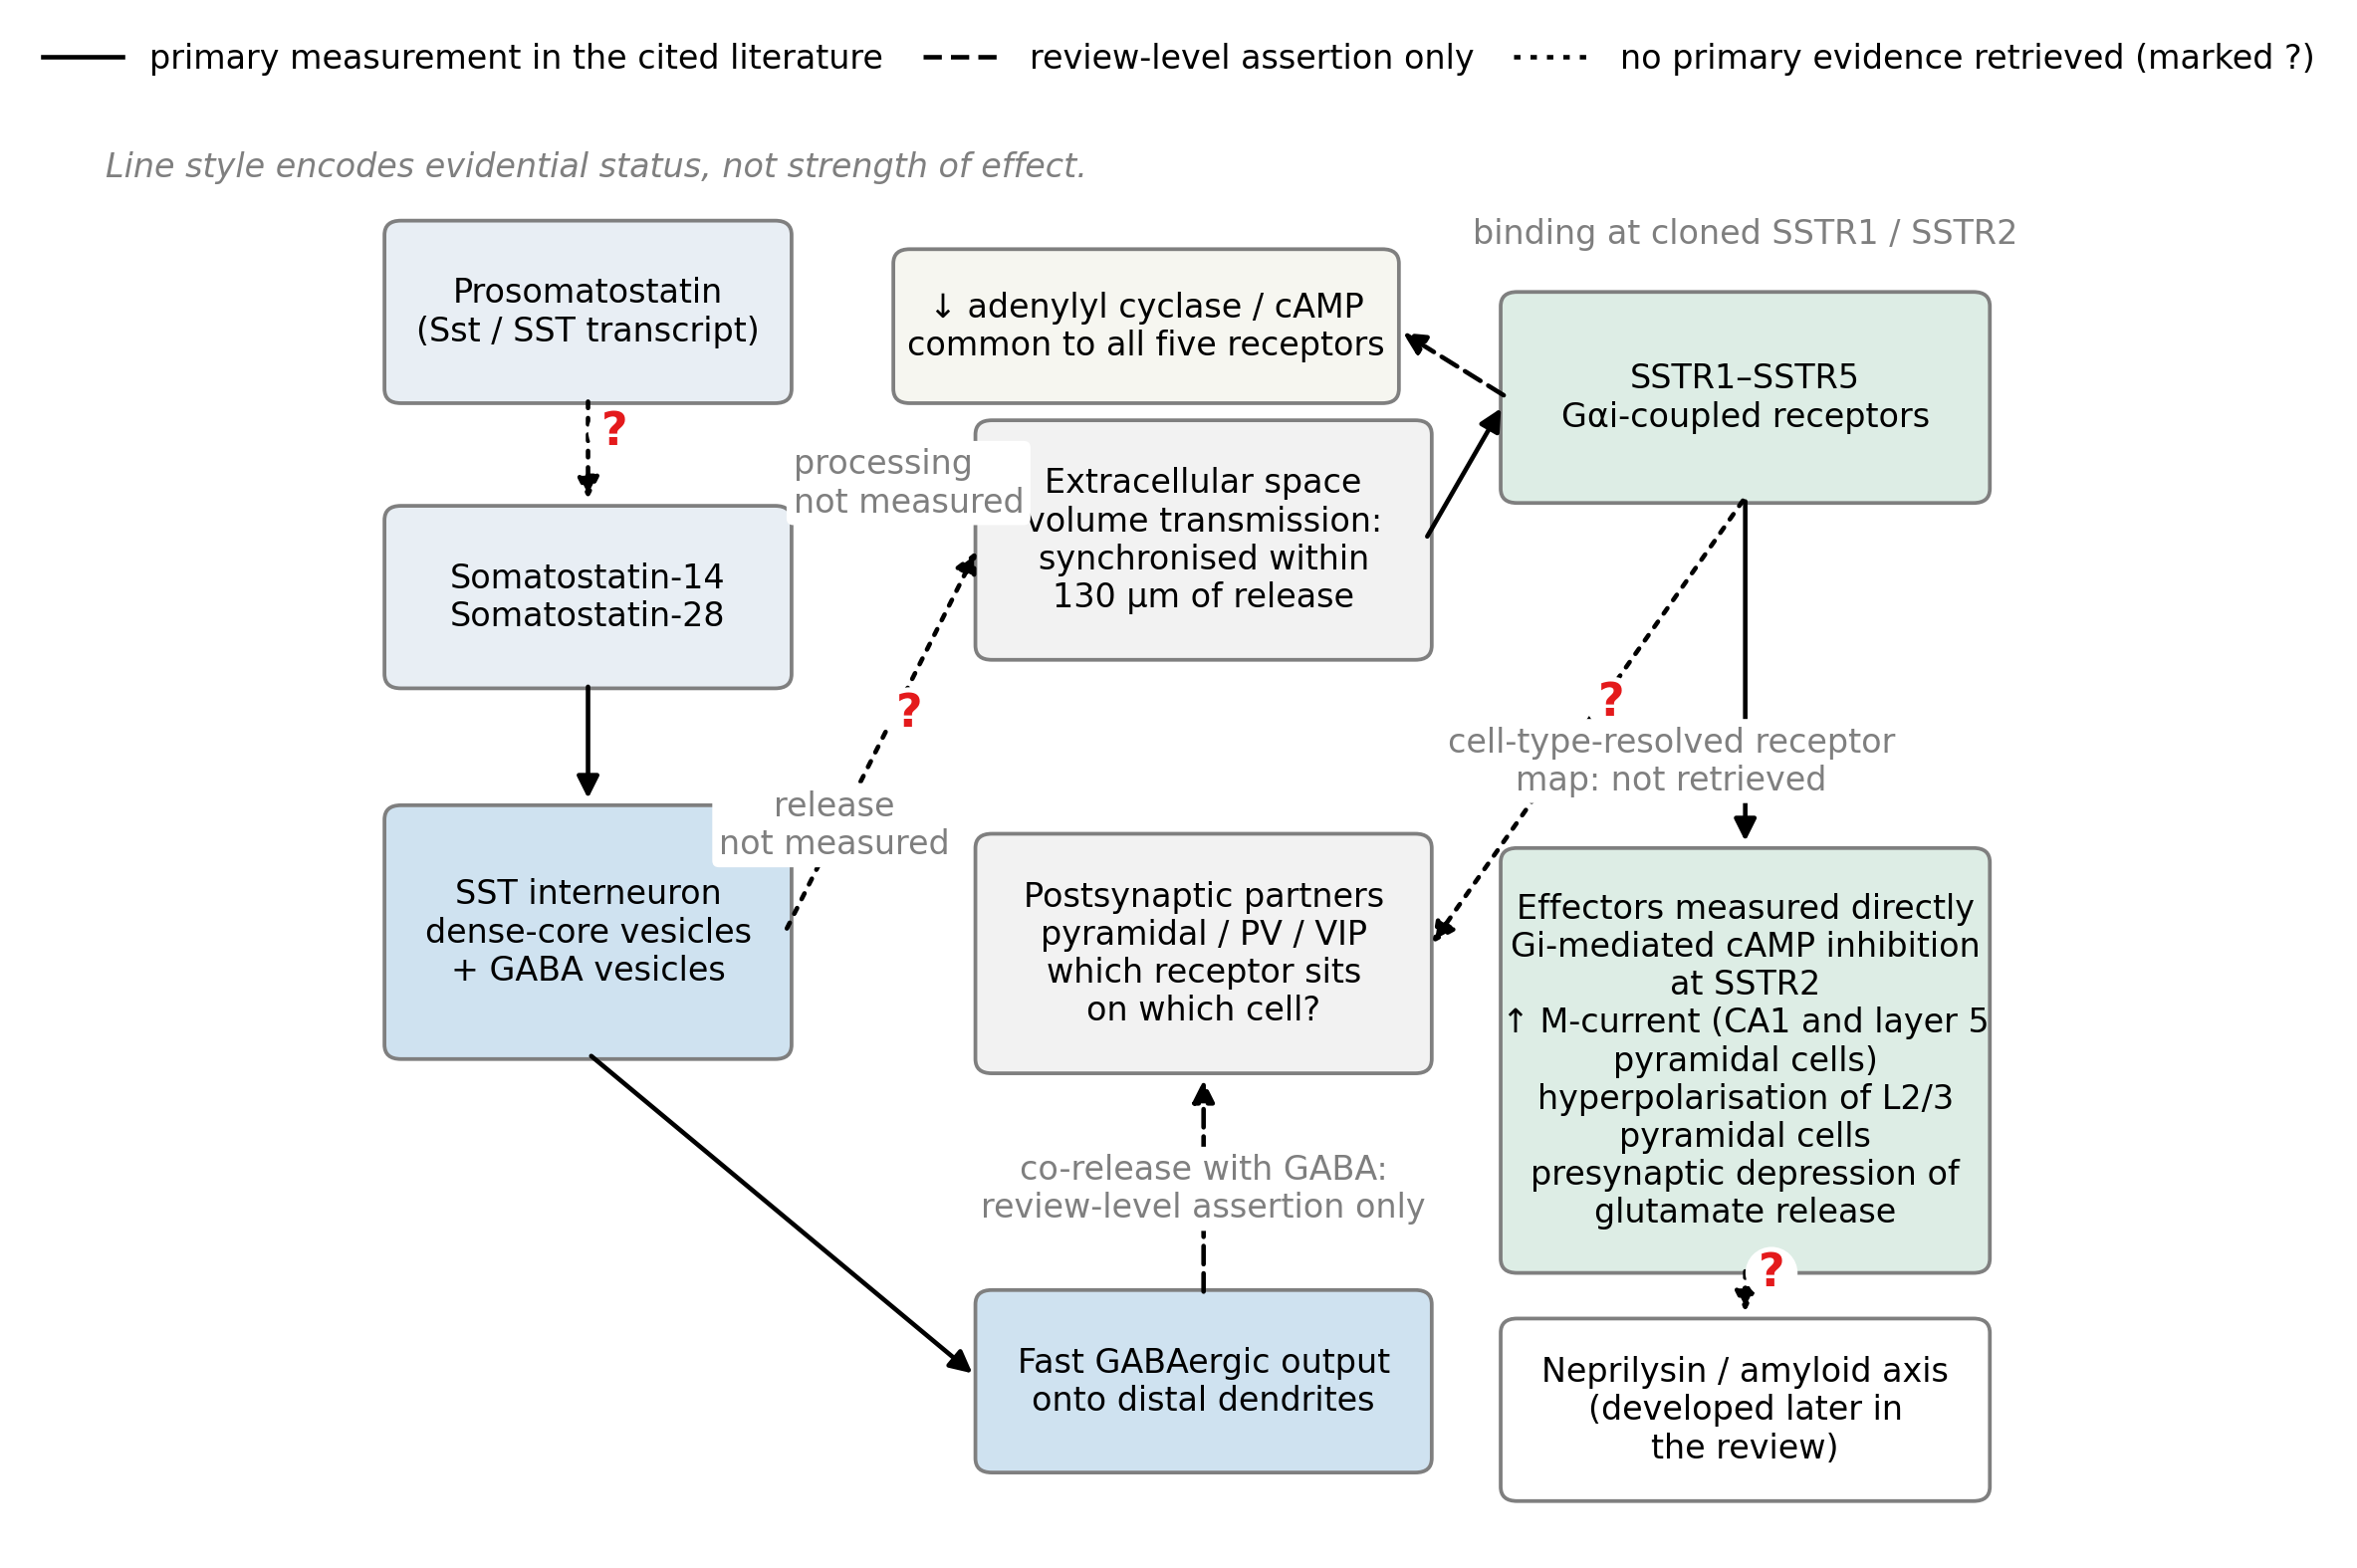
\includegraphics[width=\linewidth]{../figures/fig_sec2_sst_peptide_and_sstr_signalling.png}
\caption{\textbf{Somatostatin signalling and its evidential status.} Schematic of prosomatostatin processing to somatostatin-14 and somatostatin-28, peptide release from an SST interneuron, SSTR1--SSTR5 on postsynaptic partners, G$\alpha$i coupling and the downstream effectors. Line style encodes what supports each step rather than its importance: solid for links with a primary measurement in the literature cited here --- somatostatin-14 and somatostatin-28 binding at cloned SSTR1 and SSTR2 \citep{Yamada1992}, Gi-mediated inhibition of cAMP production at SSTR2 \citep{Heo2022}, M-current augmentation in CA1 pyramidal neurons \citep{Moore1988} and in layer V pyramidal neurons under selective SST4 agonism \citep{Kecskes2020}, hyperpolarisation of layer 2/3 pyramidal neurons by SSTR activation \citep{Brockway2023}, presynaptic depression of glutamatergic transmission \citep{Riedemann2024}, an assay demonstrating the induction and inhibition of somatostatin release in prefrontal slices \citep{Dao2019}, and synchronised transmission within 130 $\mu$m after light-triggered release of somatostatin-14 \citep{Xiong2022}; dashed for steps found only as review-level assertions, namely G$\alpha$i-dependent inhibition of adenylyl cyclase common to all five receptors and co-release of somatostatin with GABA \citep{Gunther2018}; dotted and marked with a question mark for links with no primary evidence retrieved here --- prosomatostatin processing in these neurons, activity-dependent peptide release from identified SST interneurons under physiological firing, and the cell-type-resolved distribution of SSTR1--SSTR5 across pyramidal, PV and VIP targets. The neprilysin branch is drawn dotted because no primary evidence for it is presented in this section; it is developed in \ref{sec-alzheimers}. No quantity in this diagram is a measurement except the labelled distance, which is quoted from its source.}
\label{fig-sec2-sst-peptide-and-sstr-signalling}
\end{figure}

\subsection{What the genetic toolbox actually reports}
\label{sec-02-toolbox}

Every rodent cell count in the sections that follow is bounded by what its driver line reports. Three-dimensional mapping of genetically identified interneurons through the caudoputamen found no significant anteroposterior density gradient for SST cells ($\beta$ = 4.9, p = 0.66) where parvalbumin cells showed a strong one ($\beta$ = $-$146.2, p = 3.0 $\times$ 10$^{-}$$^{1}$$^{7}$), and in the same dataset SST-immunonegative tdTomato-positive clusters in ventral striatum forced the exclusion of an entire region from the analysis \citep{Muhsinov2026}. Both reported failure modes run in the same direction --- cells the reporter counts as SST that are not SST, whether by immunoreactivity or by physiology: Sst-IRES-Cre also labels some Pvalb-like fast-spiking cells, a confound invoked to explain why large multipatch surveys detect Sst-to-Sst connections that an earlier paired-recording survey of mouse V1 did not \citep{Campagnola2022,Pfeffer2013}. Whether these lines additionally miss SST cells was not addressed by the material retrieved here. A percentage for the parvalbumin-expressing fraction that Sst-Cre labels travels with the same study that supplies the 30\% denominator, but it is attached to no quoted measurement and is therefore not reproduced here; no independent quantification of non-SST labelling was retrieved by these searches. The practical consequence is a measurement-validity problem rather than a biological one.

\begin{quote}
\noindent\textbf{Evidence conflict: is Cre-reporter density a valid proxy for SST interneuron number?}\par
One study treats a reduced density of eGFP-labelled SST cells as a change in the SST population while finding no accompanying death or oxidative-stress signal in those same cells: the proportion of eGFP-positive cells that were 3-nitrotyrosine-positive did not differ between genotypes (p = 0.9684), and no colocalisation of eGFP with cleaved caspase-3 was observed \citep{Drake2024}. The other reports SST-immunonegative tdTomato-positive cells in SST-Cre tissue, in numbers that forced an entire region to be excluded from the analysis before a genetically defined SST distribution could be described \citep{Muhsinov2026}. Stated side by side, the two disagree on whether reporter-positive density reports SST interneuron number at all --- a disagreement about what was counted rather than about the biology, and one that is unresolved. Every reporter-based cell count in the disease sections inherits it.

\end{quote}

Resolving that requires tools designed for it, and they exist: the intersectional, retrograde-tracing and layer-1-targeting transgenic strategies already described above \citep{Wu2023,Hostetler2023,Ma2006}, and Patch-seq or in-situ transcriptomic recording that assigns a recorded cell to a transcriptomic type rather than to a marker class \citep{Scala2019,Bugeon2022}. None of these was used in the older disease literature; several are rarely used in the current one.

Two limits of the evidence behind this section should be read into everything above. The literature was retrieved through a single full-text index with no citation chasing, and of the 72 papers cited here retrieval depth is recorded for 70, of which 45 were read in full text and 25 as abstracts only --- so statements of absence here, and every call of a result as unreplicated, are statements about what these searches returned rather than about what exists. And published null results here are sparse: the disconfirming material retrieved reports preserved, unchanged or non-significant outcomes rather than failed replications of a specific connectivity or receptor claim, and the targeted searches for contradictions were capped rather than exhaustive. The apparent consistency of the identity literature may therefore partly reflect what gets published. These bounds on Cre-line fidelity and on coverage reappear as a general constraint on rodent cell counts in \ref{sec-conflicts-limitations}.

Taken together, the SST label aggregates cells that differ in axonal target, postsynaptic partner, co-marker composition, developmental identity and state modulation, and it is read out by tools that count cells the marker itself does not confirm. Whether that aggregate is selectively vulnerable in neurodegenerative disease is the next question --- and in \ref{sec-selective-vulnerability} the aggregation itself turns out to be part of why the claim is hard to test.

\section{Selective Vulnerability of SST Interneurons in Aging and Neurodegeneration}
\label{sec-selective-vulnerability}

The cell class delimited in \ref{sec-sst-identity} is reached, in almost every ageing and disease study, through one of three quantities: the somatostatin peptide, the \emph{SST} transcript, or a soma scored positive for one of them. These are routinely read as interchangeable indices of one population. They are not, and the distinction organises everything that follows: the somatostatin signal declines with normal ageing by magnitudes of the same order as those disease cohorts attribute to pathology \citep{Hayashi1997,Florio1991}, though measured in different species, analytes and comparators \citep{Poirel2018}, and declines again after many acute insults, though not all \citep{Johansen1987,Freund1992}, yet the one study that counts cells independently of the peptide \citep{Komitova2013}, the marker-based counts that barely move in the same aged cortex \citep{Cha1997}, and the studies that delete the proposed vulnerability mechanisms \citep{Bouilleret2000} do not support an account of SST interneurons as intrinsically fragile. Vulnerability in this literature is better described as region- and insult-specific than as a property of the cell class.

\subsection{Age-related decline of the somatostatin signal}
\label{sec-03-aging-baseline}

Across species and assay families the somatostatin transcript falls steeply in the aged brain. In macaque, the ratio of SRIF mRNA to G3PDH mRNA decreased by 60-70\% between 2 years and more than 30 years of age, in hippocampus and in cerebral subdivisions reported as including frontal, temporal, motor, somatosensory and visual cortex \citep{Hayashi1997}. In 25-month-old rats, pre-prosomatostatin mRNA was reduced by 49\% in frontal cortex, 80\% in parietal cortex and 69\% in striatum, with no change in beta-actin gene expression \citep{Florio1991}; in Fischer 344 rats, hypothalamic somatostatin gene expression in old animals was approximately 50\% of the level in young animals while cortical expression was similar in young, middle-aged and old rats \citep{SONNTAG1990}. The two rodent series each reproduce the direction of the other but disagree region by region, and the disagreement is not cosmetic: the region that falls in one is the region that does not move in the other. What does not fall, in the same aged rodent cortex, is the number of cells; immunohistochemical counts give only slight decreases of somatostatin-immunoreactive cell numbers in parietal and occipital cortex of aged animals \citep{Cha1997}, and the hypothalamic decline was attributed by its own authors to decreased expression within specific hypothalamic nuclei rather than to a loss of somatostatin-containing neurons \citep{SONNTAG1990}. In human orbital frontal cortex, methylation of the \emph{SST} 5' UTR and first exon/intron correlates negatively with \emph{SST} expression (r = -0.48, p < 0.01 and r = -0.63, p < 0.001) - a transcriptional mechanism compatible with reduced expression in surviving cells, though the measurement is made on bulk tissue and does not localise to them \citep{McKinney2015}. The magnitudes matter downstream: the 42.4\% reduction of somatostatin expression reported in prefrontal area BA9 is a contrast between advanced dementia (CDR 5) and milder severity within one cohort rather than disease against age-matched control \citep{Poirel2018}, and it is smaller than the 49-80\% reductions that ageing alone produces in rodent cortical transcript measures \citep{Florio1991} - a different species, somatostatin peptide measured by radioimmunoassay against a transcript measure, and a different comparator. Age matching is therefore the condition under which a disease effect can be claimed at all, not a methodological courtesy.

The same ambiguity runs through every bulk readout of the human literature. Reduced cortical somatostatin-like immunoreactivity in Alzheimer tissue was established by radioimmunoassay four decades ago \citep{Davies1980} and has since been reproduced by orthogonal assays: a 10-fold downregulation of somatostatin in frontal cortex by tandem mass tag proteomics \citep{Sathe2020}, and a log fold-change of -2.2 for \emph{SST} in the precuneus by RNA sequencing of ten matched post-mortem brains \citep{Guennewig2021}. In cerebrospinal fluid the deficit is not diagnosis-specific: somatostatin was 17.5 +/- 5.0 pg/mL in dementia of the Alzheimer type against 23.1 +/- 8.2 pg/mL in age-matched controls \citep{Atack1988}, 88.0 +/- 4.1 pg/mL in 39 parkinsonian patients against 147.3 +/- 5.1 pg/mL in controls \citep{Dupont1982}, and reduced again in a separate Parkinson's disease series without correlation to dementia score \citep{Strittmatter1996a}. In both of the older cohorts the reduction was unrelated to severity or duration \citep{Atack1988,Dupont1982}, which already argues against reading the peptide as a progression marker; that evidence is assembled as a series in \ref{sec-human-evidence}. None of these measurements counts a cell; \ref{fig-sec3-marker-level-readouts-transcript-peptide-csf} sets the three readout families side by side. Where the cellular correlate has been examined directly, the morphological substrate of reduced cortical somatostatin and neuropeptide Y content was reported to be distortion and reduction of fibre plexuses rather than cell disappearance \citep{Kowall1988}, consistent with somatostatin-immunoreactive processes residing within neuritic plaques \citep{Morrison1985} and with the correlation between somatostatin and choline acetyltransferase deficits in association areas 9 and 22 \citep{Dournaud1995}. Much of this historical postmortem and cerebrospinal-fluid series was read here at abstract level only - 26 of 80 findings in this literature were available as full text - so assay details that would adjudicate between these readings are frequently not in hand.

\begin{quote}
\noindent\textbf{Evidence Conflict}\par
\textbf{Transcript versus cell count in the same aged rodent cortex.} \citet{Florio1991} report pre-prosomatostatin mRNA reductions of 49-80\% across aged rat forebrain, while \citet{Cha1997} report only slight decreases in somatostatin-immunoreactive cell numbers in aged rat cortex. The disagreement is one of measurement modality and of what was counted, not of direction: a transcript pool can collapse in neurons that remain in place. Status: resolved by method, in the sense that the two measures are not measuring the same thing - but the resolution removes the cell-loss reading from the ageing literature rather than reconciling it.

\end{quote}

\begin{figure}[H]
\centering
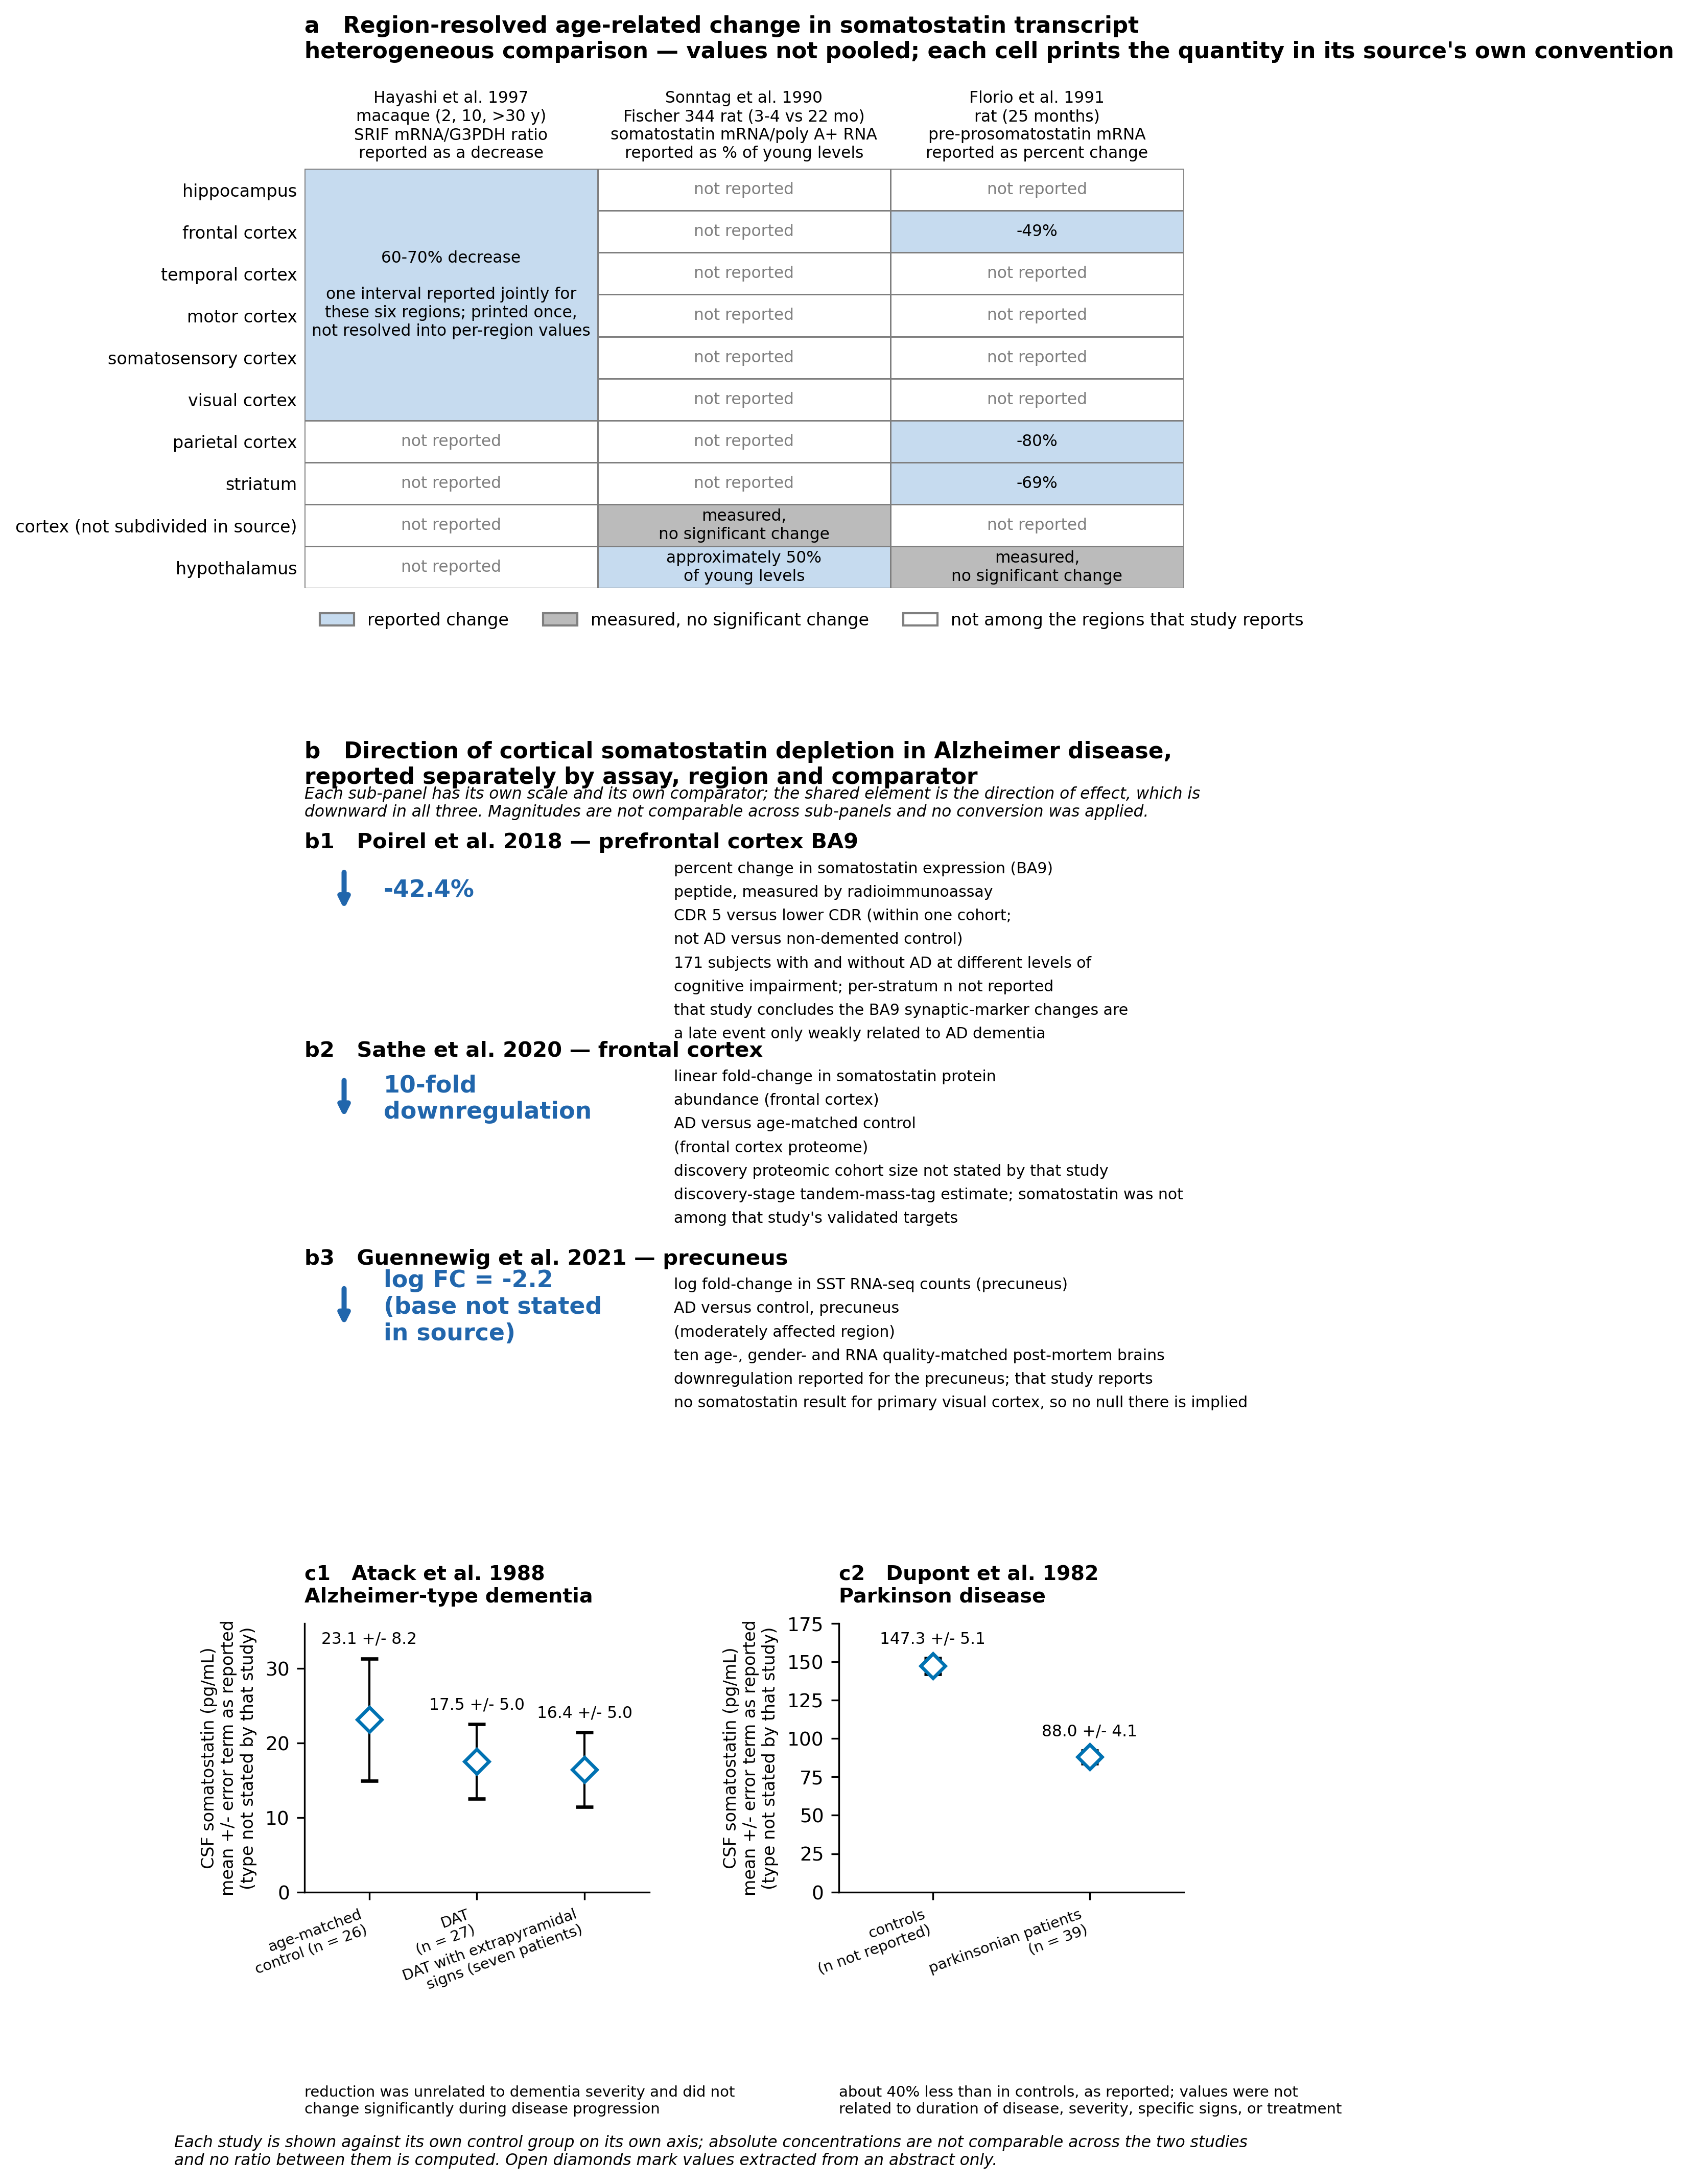
\includegraphics[width=\linewidth]{../figures/fig_sec3_marker_level_readouts_transcript_peptide_csf.png}
\caption{\textbf{Three marker-level readouts, none of which counts a cell.} (a) Region-resolved age-related change in somatostatin transcript. Cells print each quantity in its source's own convention and no conversion between conventions was applied; \citet{SONNTAG1990}'s hypothalamic cell is a remaining level (approximately 50\% of young levels), not a signed change. The macaque 60-70\% figure is one interval covering the hippocampus and frontal, temporal, motor, somatosensory and visual cortex jointly; it is printed once in a single cell spanning those six rows and is never repeated into individual region rows, and parietal cortex and striatum are not among the regions that study reports, so its cell does not extend to those rows \citep{Hayashi1997}. The two rat studies disagree region by region - somatostatin transcript falls in hypothalamus but not cortex in \citet{SONNTAG1990}, and in frontal cortex, parietal cortex and striatum but not hypothalamus in \citet{Florio1991} - and both measured nulls are shown as cells; this is a cross-study conflict, not convergent evidence. Quantification is stated only as far as the sources state it: a SRIF mRNA/G3PDH ratio \citep{Hayashi1997}; somatostatin mRNA/poly A+ RNA, with in situ hybridization supporting the statement that the hypothalamic decrease reflects reduced expression within specific nuclei \citep{SONNTAG1990}; and pre-prosomatostatin mRNA levels with beta-actin gene expression unchanged, no quantification method being stated in that study \citep{Florio1991}. The three normalizers are not interchangeable and none is an absolute transcript level. Species and ageing windows differ (macaque at 2, 10 and >30 years; Fischer 344 rat at 3-4 versus 22 months; rat at 25 months); there is no common age scale and no pooled ageing effect. No per-group sample size is reported in any source. (b) Direction of cortical somatostatin depletion in Alzheimer disease, one sub-panel per study, each on its own scale: percentage change in somatostatin expression, linear fold-change in protein abundance, and logarithmic fold-change in RNA-seq counts. Magnitudes must not be compared across sub-panels; no conversion was applied, because the base of the logarithmic fold-change is not stated in the source. The 42.4\% value is somatostatin peptide measured by radioimmunoassay in that study, and that contrast is CDR 5 against lower dementia severity within one cohort of 171 subjects, not against non-demented controls - that study concludes the BA9 synaptic-marker changes are a late event only weakly related to dementia \citep{Poirel2018}. The largest magnitude shown is a discovery-stage proteomic estimate, and somatostatin was not among that study's validated targets \citep{Sathe2020}. The somatostatin downregulation of \citet{Guennewig2021} is reported for the precuneus; that study describes the two regions' transcriptomic signatures as similar and reports no somatostatin result for primary visual cortex, so no null in that region should be inferred. All three are bulk-tissue measures and none separates peptide or transcript downregulation from loss of cells. (c) Cerebrospinal-fluid somatostatin in Alzheimer-type dementia and in Parkinson disease, each study in its own sub-panel against its own control group and never on a shared axis: control means are 23.1 pg/mL \citep{Atack1988} and 147.3 pg/mL \citep{Dupont1982}, a difference neither study explains, since neither abstract states the assay used; it must not be attributed to different radioimmunoassays or standards, and no ratio between the two is computed. Neither abstract states whether its reported +/- term is a standard deviation or a standard error, so the marks are drawn as plain reported ranges with no type named and no conversion attempted, and the two sub-panels' error marks are not of established comparable kind. Group sizes are reported differently: 26 control, 27 with dementia of the Alzheimer type and seven with extrapyramidal signs \citep{Atack1988}; 39 parkinsonian patients with control group size not reported \citep{Dupont1982}. Only the second study states a within-study percentage (about 40\% less than in controls); none is printed for the first because its sources state none. This is a cross-disease comparison against separately constituted control groups, not a replication, and in both studies the reduction was unrelated to disease severity or duration. Open diamonds mark values extracted from an abstract only. Values are not pooled anywhere in this figure.}
\label{fig-sec3-marker-level-readouts-transcript-peptide-csf}
\end{figure}

\subsection{The hilar lesion model and what it does and does not generalise}
\label{sec-03-hilar-lesion}

The strongest demonstration of somatostatin-cell vulnerability anywhere in this literature comes from the dentate hilus after acute insult, and it is genuinely strong. Transient forebrain ischaemia in rat produced a significant 60\%-80\% loss of hilar and CA3c somatostatin neurons, quantitated at day 1, 2, 3 and 4, with damage significant on the second postischemic day and preceding the delayed loss of CA1 neurons \citep{Johansen1987}. Two minutes of ischaemia in gerbil - too brief to kill CA1 pyramidal neurons - caused a selective 40\% loss of hilar somatostatin neurons at 1 day and 60\% at 7 days, with no loss after 1 minute and almost complete loss after repeated 2-minute episodes \citep{Matsuyama1993}. After status epilepticus the hilar somatostatin-containing cells were the most vulnerable cell type while parvalbumin- and calbindin-containing nonprincipal neurons were remarkably resistant \citep{Freund1992}, and the magnitude was extended in epileptic mice, in which hilar somatostatin interneuron numbers fell to 18\% of controls \citep{Hofmann2016}. That ranking is not reproduced everywhere: in progressive-seizure animals hilar parvalbumin- AND somatostatin-immunoreactive neurons were almost completely eliminated together, while non-progressive animals retained both unilaterally \citep{Gorter2001}, so in that model the loss is not confined to the somatostatin population. Traumatic and ischaemic lesions converge on the same subfield: hilar cell loss after fluid-percussion injury included somatostatin-immunoreactive neurons, with irreversible hilar injury within 4 hours of impact \citep{Lowenstein1992}, and hilar and CA3 interneuronal damage after four-vessel occlusion extended over a wider dorsoventral range than CA1 damage \citep{Hsu1993}, with spiny calretinin-containing hilar neurons degenerating on the same early schedule \citep{Freund1993}. Unbiased stereology in two acquired-epilepsy models resolves the pattern as subtype- and subfield-specific rather than global: neuropeptide Y-immunoreactive dentate neurons fell to 33-37\% of control (p < 0.01) while parvalbumin-immunoreactive neurons in the ipsilateral CA1 were at 80\% remaining (p < 0.05) \citep{Huusko2013} - both values are from the post-status-epilepticus arm of that study, which counted somatostatin neurons as well, and neuropeptide Y is co-expressed with somatostatin in only part of this population, so it is a proxy and not a substitute. This is a replicated, cross-species, cross-insult result about a hilar population - not about SST interneurons in general, as \ref{fig-sec3-sst-depletion-across-insults} makes plain.

Its generality fails in three directions at once. After diffuse mild traumatic brain injury, axotomy within the somatostatin population was rare, representing only 10\% of the axotomy occurring in GAD67-positive swellings, and somatostatin-to-pyramidal synaptic efficacy was enhanced rather than degraded \citep{Harris2022}; and the two remaining injury models disagree with each other: controlled cortical impact yields significant ipsilateral SST interneuron loss together with a roughly fourfold reduction of long-range input to hippocampal SST interneurons, the input reduction not accompanied by cell loss in the distant regions supplying it \citep{Frankowski2022}, whereas lateral fluid percussion injury yields heterogeneous hippocampal interneuron changes and no obvious loss of any interneuron subset in motor cortex \citep{Carron2019}. Whether traumatic injury depletes this class consistently is therefore unsettled, and the discrepancy tracks the model and the region sampled. In striatum the class is repeatedly spared, by peptide content and by cell count alike: somatostatin and neuropeptide Y concentrations were unchanged despite a significant 25\% depletion of substance P-like immunoreactivity and GABA after transient forebrain ischaemia in gerbil striatum \citep{Uemura1990}, the same peptides were unaffected within areas of ischaemic damage in neonatal rat \citep{Ferriero1988}, somatostatin-immunoreactive and cholinergic neurons were relatively preserved in areas of severe neuronal loss in adult gerbil \citep{Chesselet1990}, and somatostatin interneuron numbers were no different from the contralateral hemisphere at 3 and 14 days after mild focal ischaemia \citep{Katchanov2003}. Sparing is not universal there either - striatal somatostatin/NPY interneurons are highly vulnerable to quinolinic acid while cholinergic interneurons are highly resistant \citep{FigueredoCardenas1998} - which is the point: the answer changes with the insult, not with the marker. Developmental and perinatal insults add a third pattern, in which the marker falls without the cells going missing \citep{Komitova2013}; a multi-hit neonatal injury model gives a persistent 32\% reduction in the density of somatostatin-immunoreactive interneurons in prefrontal cortex, confined to upper layers, with no marker-independent count reported \citep{Lacaille2019}, and in preterm fetal sheep somatostatin interneuron numbers fell in caudate, putamen, intragyral white matter and entorhinal cortex while the rest of cortex was virtually unaffected \citep{Ardalan2019}. Reported null results include the aluminium tangle model in rabbit cortex, in which cortical somatostatin and NADPH-diaphorase neurons were unaffected \citep{Kowall1989}.

\begin{quote}
\noindent\textbf{Evidence Conflict}\par
\textbf{Vulnerable class or resilient class?} \citet{Hofmann2016} report hilar somatostatin interneurons reduced to 18\% of control in epileptic mice; \citet{Harris2022} report that after mild traumatic brain injury axotomy is largely confined to parvalbumin cells, with somatostatin axotomy representing only 10\% of that in GAD67-positive swellings, and somatostatin output enhanced. A parallel disagreement runs between hilus and striatum under acute insult: hilar somatostatin cells are the most vulnerable type after status epilepticus, a death pattern its authors describe as resembling ischaemic damage \citep{Freund1992}, while striatal somatostatin content is unchanged after transient forebrain ischaemia \citep{Uemura1990}. The axis is model construct and circuit context rather than measurement: the same marker yields opposite conclusions about vulnerability in different regions and insults. Status: resolved by method, in favour of insult- and region-specificity over class-intrinsic fragility. The inventory of these disagreements is assembled in \ref{sec-conflicts-limitations}.

\end{quote}

\begin{figure}[H]
\centering
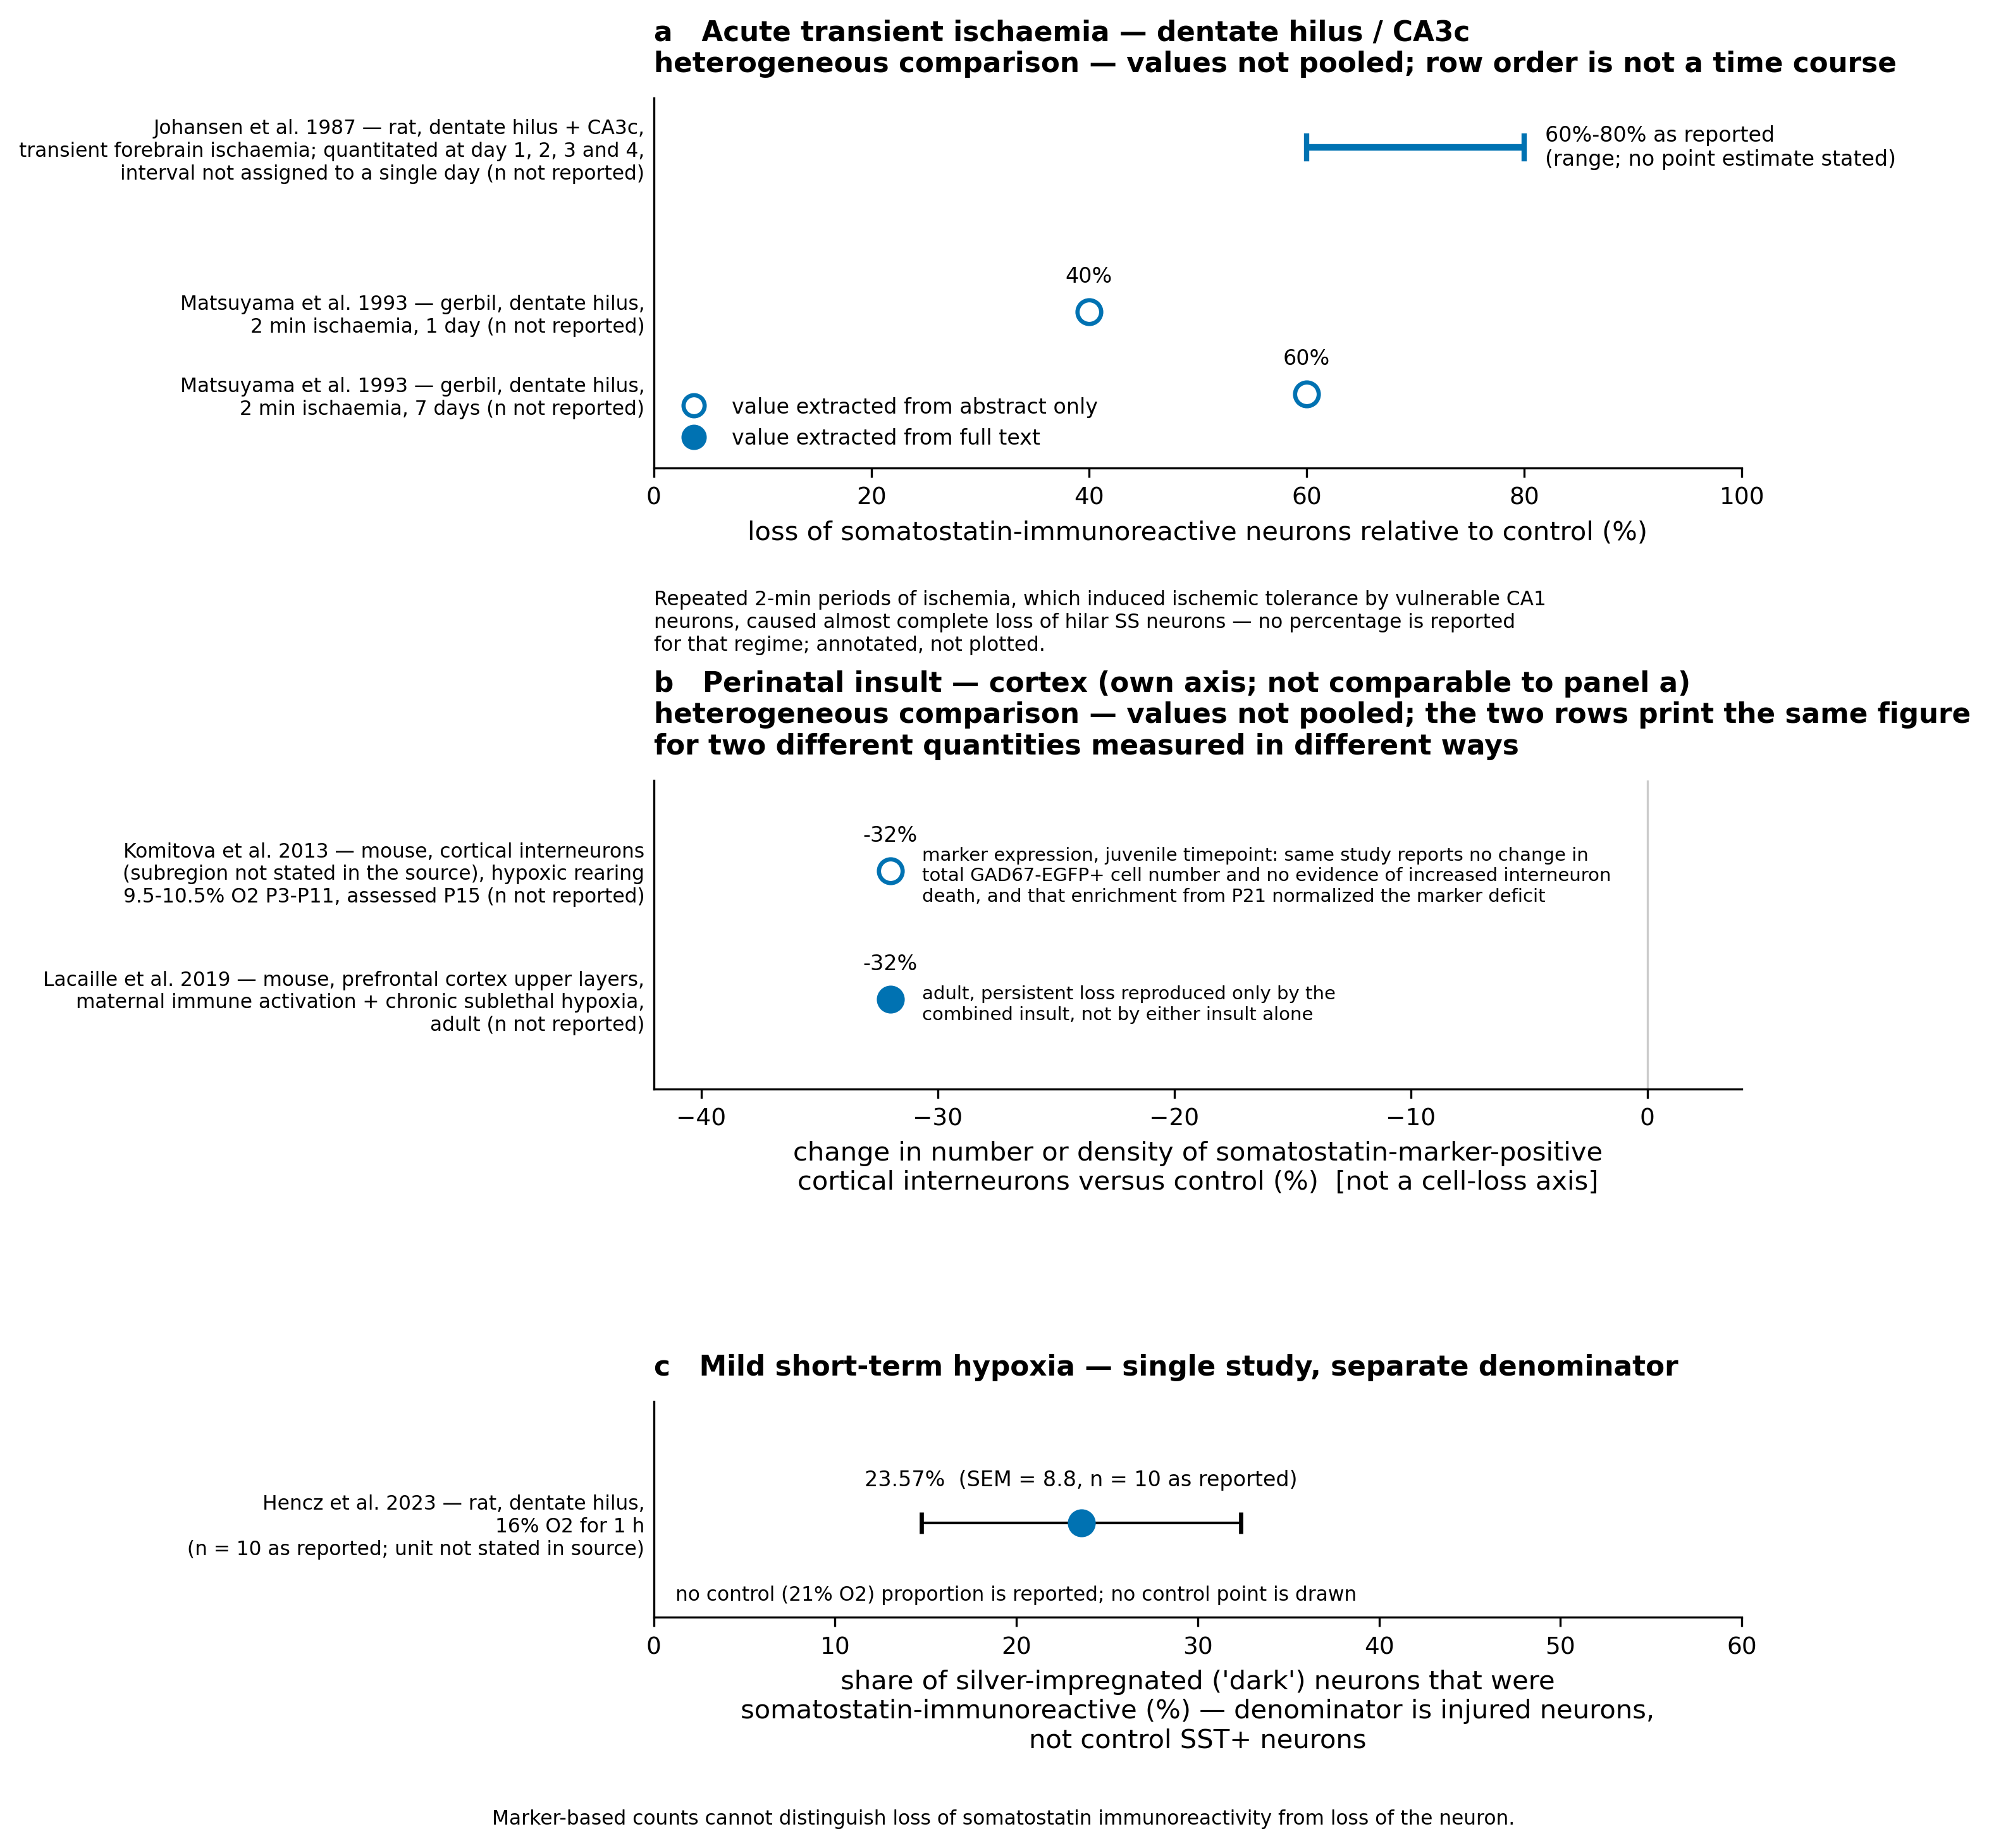
\includegraphics[width=\linewidth]{../figures/fig_sec3_sst_depletion_across_insults.png}
\caption{\textbf{Reported somatostatin depletion after acute and developmental insult, by region and model.} Panels have independent axes; no value is ordered against or compared with a value in another panel. (a) Loss of somatostatin-immunoreactive neurons relative to control after acute transient ischaemia. \citet{Johansen1987} is drawn as the reported 60\%-80\% interval rather than a point estimate; the source does not state what the width of that interval represents, and it is not attributed here to region pooling, survival time or dispersion. Survival times are not matched: that study quantitated somatostatin-immunopositive cell somata at day 1, 2, 3 and 4 after cerebral ischaemia and assigns the interval to no single day, reporting that damage was significant on the second postischemic day, whereas the two rows from \citet{Matsuyama1993} are explicitly 1 day and 7 days. Row order is not a time course. \citet{Matsuyama1993} used both immunocytochemistry and in situ hybridization histochemistry and the abstract does not state which modality yields the 40\% and 60\% figures, so the counting unit of those rows is not established as identical to the immunopositive cell somata counted by \citet{Johansen1987}. Neither abstract states the denominator against which percentage loss was computed. Species and insults differ (rat transient forebrain ischaemia; gerbil 2-minute transient ischaemia) and are not interchangeable models. That study also reports almost complete loss of hilar somatostatin neurons after repeated 2-minute ischaemic periods; no percentage is given for that regime, so it is annotated and not plotted. Per-group sample sizes are not reported in either source and error terms are heterogeneous (one P value, none), so no error bars are drawn. (b) Change in cortical somatostatin-marker-positive interneurons after perinatal insult, on its own axis, not aligned with or comparable to panel (a); the axis is change in marker-positive cells, not cell loss. \citet{Komitova2013} counted interneurons with immunohistochemically detectable somatostatin at P15 after hypoxic rearing at 9.5-10.5\% O2 from P3 to P11; that study reports no change in total GAD67-EGFP+ interneuron number and no evidence of increased death, attributing the decrease to reduced marker expression rather than cell loss, and reports that an enriched environment from P21 until adulthood normalized phenotypic marker expression without affecting total interneuron numbers. Its 32\% figure is reported for cortical interneurons with no subregion named - the frontal neocortex figure in that study is a separate measurement, total GABA content decreased by 31\% - so no cortical subregion is attributed to this value. \citet{Lacaille2019} reports a persistent adult decrease in the density of somatostatin-immunoreactive interneurons in prefrontal cortex, confined to upper cortical layers and produced only by maternal immune activation combined with chronic sublethal hypoxia, not by either insult alone. The two rows print the same figure for two different quantities measured in different ways; the coincidence is not evidence of a shared mechanism or of replication, and counts and densities are not interchangeable because density can fall without a change in cell number. The two rows are shown on one axis, each annotated with the quantity it represents. Per-group sample sizes are unavailable for both studies. (c) Somatostatin-immunoreactive share of silver-impregnated injured neurons after 1 hour of mild hypoxia at 16\% O2 in rat dentate hilus \citep{Hencz2023}. The denominator is injured neurons, not control somatostatin neurons, so a larger value does not mean greater somatostatin neuron loss and the value is not on a loss axis. No 21\% O2 control proportion of somatostatin-immunoreactive dark neurons is reported, so 23.57\% cannot be read as an increase relative to control and no control point is drawn. The source states n = 10 as reported and does not name the unit counted; SEM = 8.8 is reported as such. Open markers mark values extracted from an abstract only; filled markers mark full-text sources. All marker-based counts in this figure conflate loss of somatostatin immunoreactivity with loss of the neuron, and no values are pooled.}
\label{fig-sec3-sst-depletion-across-insults}
\end{figure}

\subsection{Candidate cell-intrinsic mechanisms and their evidential status}
\label{sec-03-mechanisms}

The mechanistic menu offered for hilar and cortical somatostatin-cell vulnerability is short and, measured against what was actually tested, thinly supported; \ref{fig-sec3-vulnerability-mechanisms-and-their-evidence} audits it mechanism by mechanism. The dominant cell-intrinsic account is buffer deficiency: hilar somatostatin-containing cells and CA3 pyramidal cells contain neither parvalbumin nor calbindin-D28K, an observation made in the same preparations that established their ischaemic vulnerability \citep{Freund1990,Freund1992}. The available causal test runs the other way. Parvalbumin-deficient, parvalbumin/calbindin-deficient and parvalbumin/calretinin-deficient mice show no difference in hippocampal cytoarchitecture or in the number, distribution or morphology of interneurons \citep{Bouilleret2000}, and parvalbumin content does not protect striatal interneurons from quinolinic acid \citep{FigueredoCardenas1998}. An excitotoxic-signalling account has one experimental anchor - the identification of STEP-dependent suppression of ERK/MAPK survival signalling as what renders hilar somatostatinergic interneurons vulnerable to status epilepticus \citep{Choi2007} - which no replication was retrieved for in the nineteen years since, and which should be read as a single study. Seizure-linked metabolic stress has been measured in identified cells: pimonidazole immunoreactivity, probing hypoxia, was present in neuropeptide Y- and somatostatin-labelled neurons, and counts of pimonidazole-positive neurons rose with status epilepticus duration (P < 0.01, 120 versus 60 and 30 minutes) \citep{Gualtieri2012}. Transcriptional vulnerability to a neuroendocrine stressor has likewise been measured at cell-type resolution in one study, with very few gene changes in pyramidal neurons compared with somatostatin neurons after corticosterone exposure \citep{Lin2015} - but in young adults under chronic stress, not in aged or degenerating tissue, so its extension to ageing is extrapolation.

\begin{quote}
\noindent\textbf{Evidence Conflict}\par
\textbf{Does missing calcium buffering explain hilar somatostatin-cell vulnerability?} \citet{Freund1990} report that hilar somatostatin cells contain neither parvalbumin nor calbindin and degenerate earliest, but conclude against any consistent relationship between calcium-binding-protein content and ischaemic vulnerability, since CA3 pyramidal cells are equally buffer-free and resistant; \citet{Bouilleret2000} find that genetically deleting those buffers, singly and in combination, leaves interneuron number, distribution and morphology unchanged. The first is correlative and the second is a direct test, so the inference from marker absence to fragility is not supported by the retrieved evidence, while remaining the most frequently repeated explanation. Status: open - deletion of the buffers is not the same experiment as deletion of the buffers plus an insult, and that experiment was not retrieved by these searches.

\end{quote}

What is missing is more striking than what is present. No primary per-cell-type measurement of oxygen consumption, ATP demand or reactive-oxygen load in identified somatostatin interneurons was retrieved by these searches, so the metabolic-load explanation - the one most often repeated as the reason this class is fragile - rests on inference from bulk and transcriptomic association rather than on measurement; it is carried forward as an open question in \ref{sec-conflicts-limitations}. No study retrieved here measured calcium transients or buffering capacity in identified somatostatin cells under degenerative conditions, so the buffer account is supported only by marker expression. The ER-stress account is in the same position: no measurement of the unfolded protein response or of oxidative load in identified somatostatin interneurons of aged animals was retrieved by these searches, so its operation in ageing is extrapolated from chronic stress in young adults. Direct loss-of-function evidence that reduced BDNF/TrkB signalling causes somatostatin interneuron loss in the aged brain was likewise not retrieved: what exists is co-decline, with somatostatin and BDNF transcripts falling together in aged macaque brain \citep{Hayashi1997} and their promoters hypermethylated in parallel in aged human cortex \citep{McKinney2015}. Receptor-level ageing changes on the cells themselves are better measured: somatic GluN2B puncta density on hippocampal O-LM interneurons declines between 3 and 16 months with GluN1 unchanged \citep{Gramuntell2021}, while a preprint reports reduced GluN1 puncta density and size on cortical Martinotti cells in older animals, most pronounced in females \citep{SanchezMoreno2025}, while mGlu1 activation depolarizes all prelimbic somatostatin interneurons tested in young adult cortex, with no ageing comparison reported \citep{Maksymetz2021}. Genotype and sex modulate the ageing trajectory - female apoE4 knock-in mice lose hilar somatostatin-positive interneurons faster than apoE3 controls (genotype F(1,54) = 23.85, p < 0.005) \citep{Leung2012} - and loss of SSTR2 from human locus coeruleus from Braak stages III/IV onward, with \emph{Sstr2} deletion alone causing progressive noradrenergic degeneration \citep{Adori2015}, proposes a receptor-side mechanism for which no replication was retrieved by these searches in the eleven years since.

\begin{figure}[H]
\centering
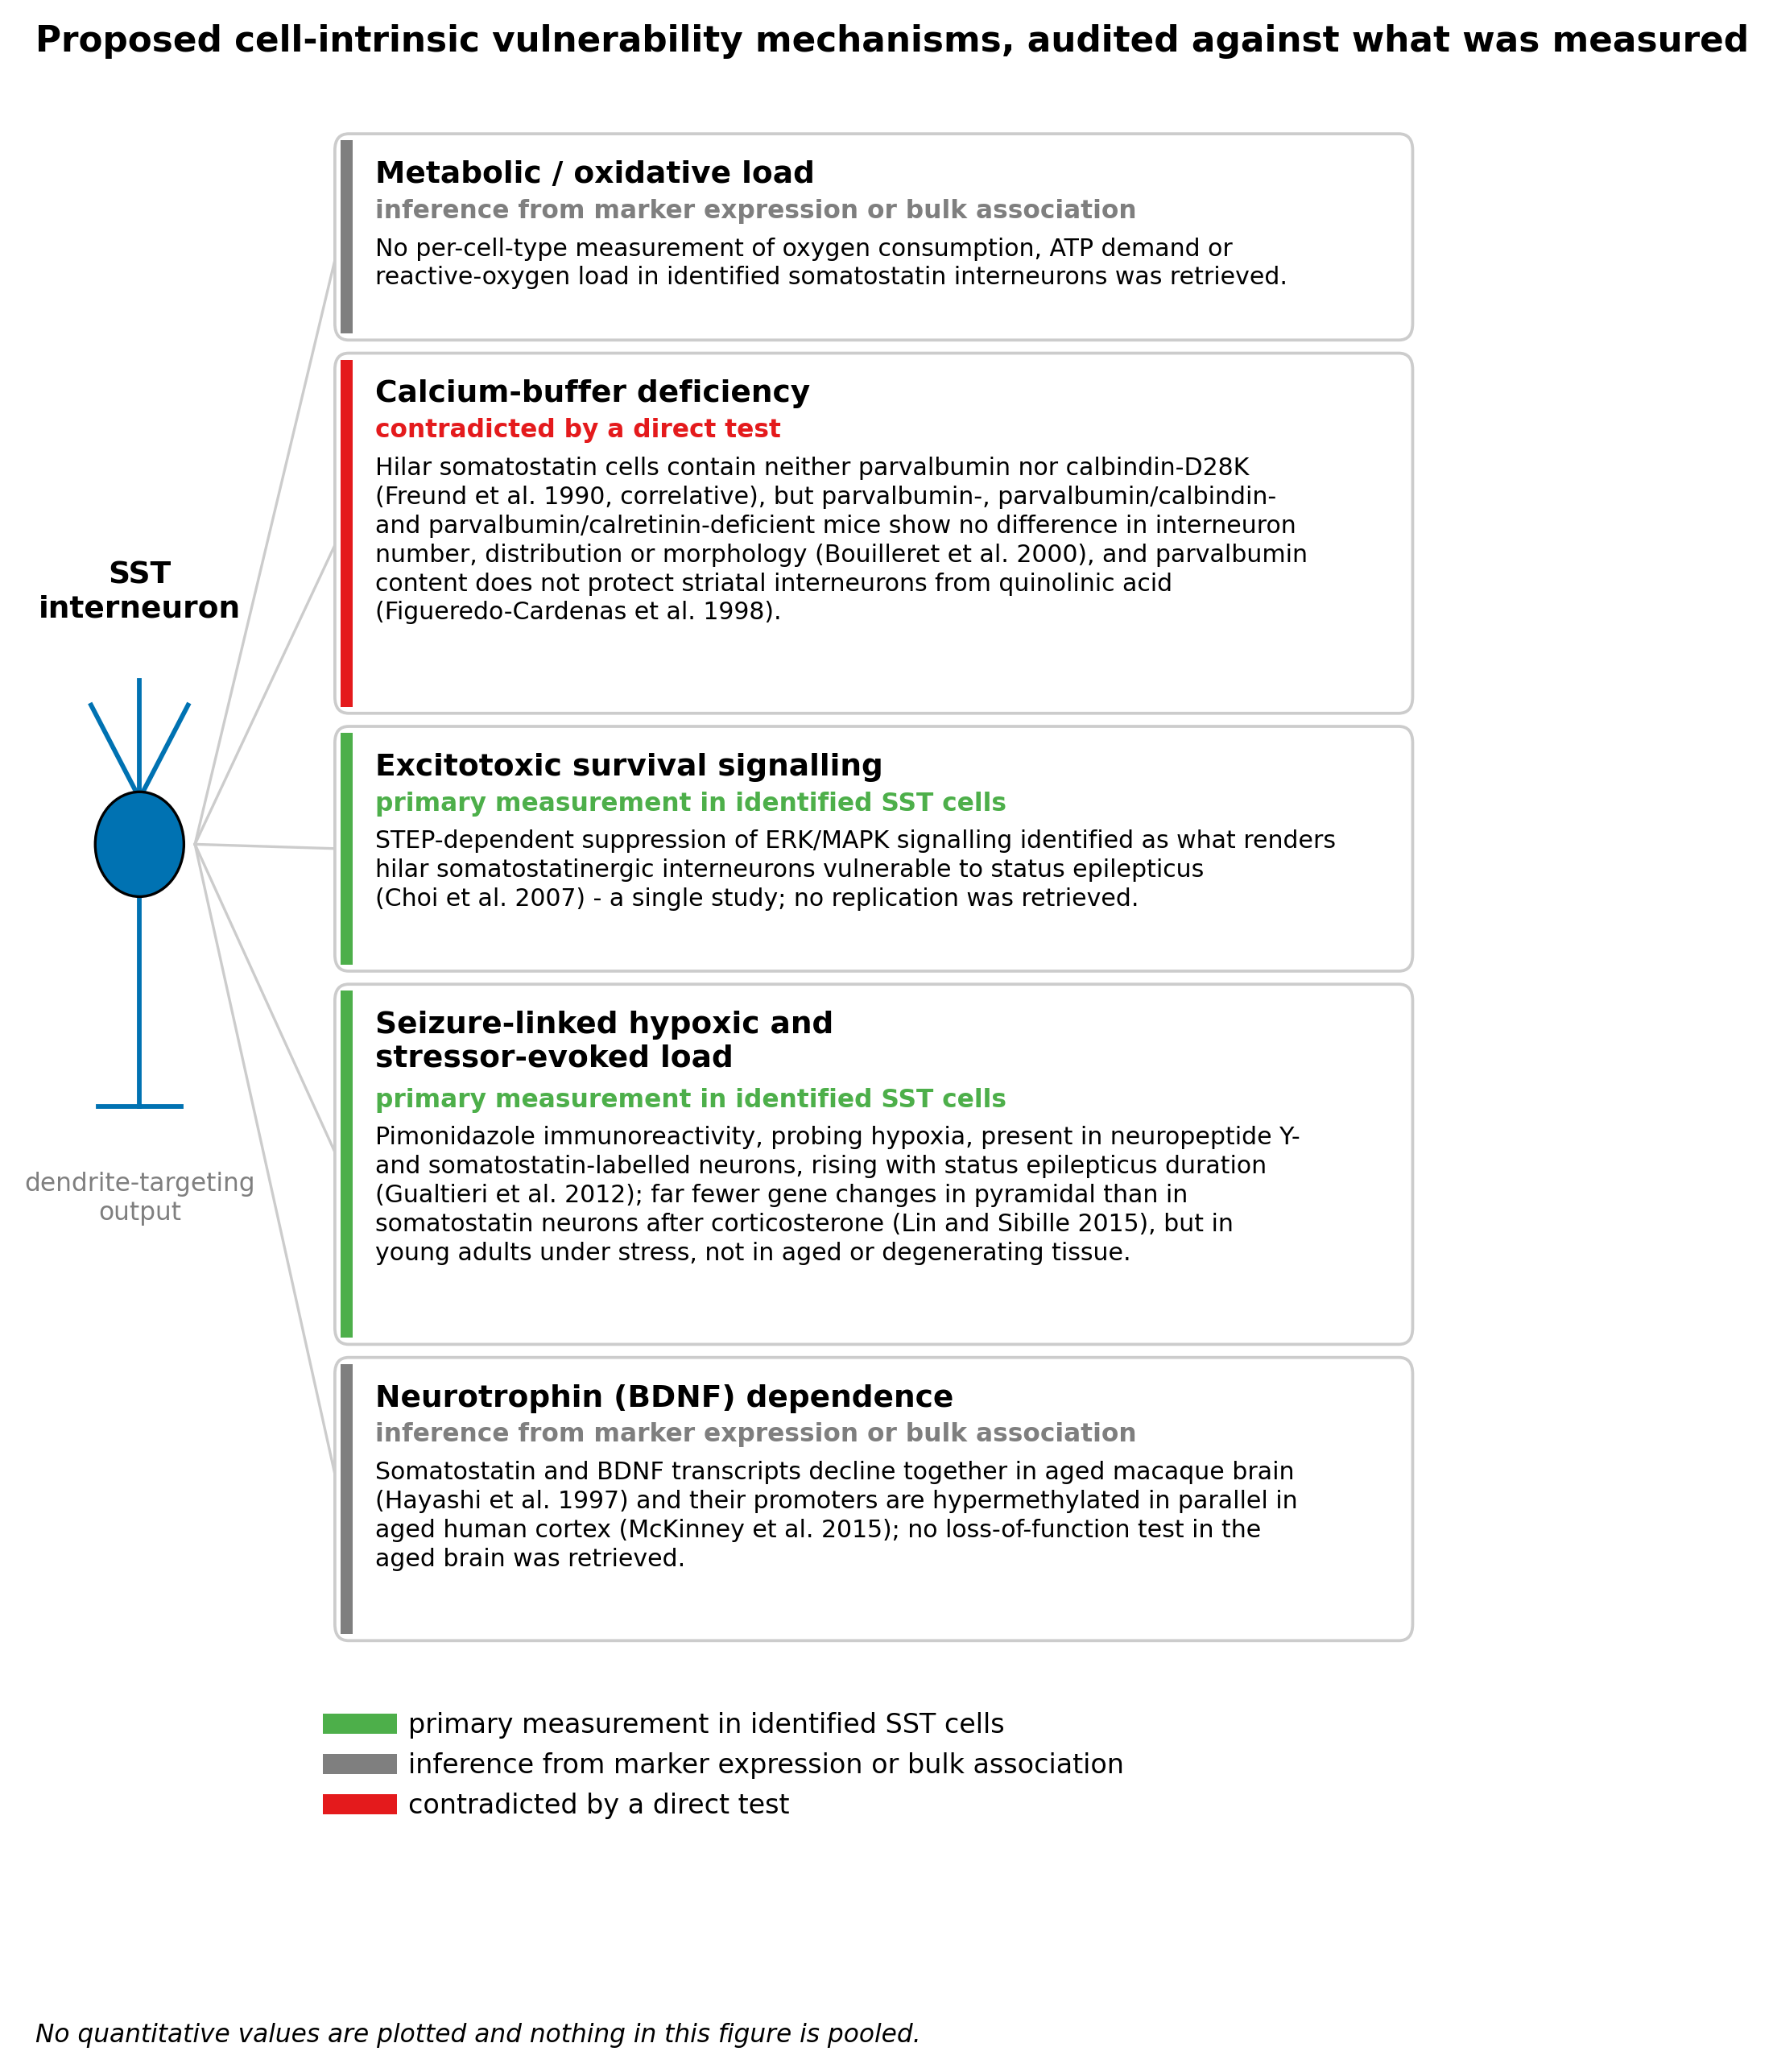
\includegraphics[width=\linewidth]{../figures/fig_sec3_vulnerability_mechanisms_and_their_evidence.png}
\caption{\textbf{Proposed cell-intrinsic vulnerability mechanisms, audited against what was measured.} Five explanations offered for somatostatin interneuron vulnerability, each tagged by the strongest evidence retrieved for it: primary measurement in identified somatostatin cells, inference from marker expression or bulk association, or contradiction by a direct test. Seizure-linked hypoxic stress is measured in identified neuropeptide Y- and somatostatin-labelled cells \citep{Gualtieri2012} and stressor-evoked transcriptional vulnerability at cell-type resolution \citep{Lin2015}, though the latter in young adults rather than aged tissue. The calcium-buffer account is marked as contradicted: the correlative observation that hilar somatostatin cells contain neither parvalbumin nor calbindin \citep{Freund1990} is set against the absence of any interneuron loss or morphological change in parvalbumin-, parvalbumin/calbindin- and parvalbumin/calretinin-deficient mice \citep{Bouilleret2000} and against the failure of parvalbumin content to protect striatal interneurons from quinolinic acid \citep{FigueredoCardenas1998}. The excitotoxic-signalling badge marks a single unreplicated study \citep{Choi2007}. Metabolic and oxidative load carries no badge for primary measurement because no per-cell-type measurement of metabolic or oxidative load in identified somatostatin interneurons was retrieved by these searches; neurotrophin dependence rests on correlated co-decline of somatostatin and BDNF transcripts \citep{Hayashi1997,McKinney2015} with no loss-of-function test in aged brain retrieved. No quantitative values are plotted and nothing in this figure is pooled.}
\label{fig-sec3-vulnerability-mechanisms-and-their-evidence}
\end{figure}

\subsection{Cross-disease magnitude, and why the convergence is partly artefactual}
\label{sec-03-magnitude}

Assembled across models, reported depletion runs from roughly a fifth of controls remaining to no change at all, and the position a study occupies in that range tracks its denominator and its labelling strategy more closely than its disease. At the severe end, hilar somatostatin interneurons fell to 18\% of controls in epileptic mice \citep{Hofmann2016} and stereological counting in PS1xAPP hippocampus gave a 50-60\% diminution of somatostatin-immunopositive neurons preceding pyramidal cell loss \citep{Ramos2006}. In the middle sit genetic-injury models that count a reporter-defined subset rather than the whole population: granule-cell \emph{Pten} deletion reduced eGFP-SST cell density in hilus (4,395 +/- 182 to 3,411 +/- 322 cells/mm3, p = 0.0334) and CA1 but not CA3 \citep{Drake2024}, and targeted ablation, in which the depletion is the manipulation rather than a measured consequence of pathology, reduced SOM-positive cells in dentate gyrus and CA3 while sparing CA1 \citep{Nagarajan2023}. In human tissue the same spread appears across techniques, and it brackets zero: stereological counting gives a 50\% reduction in the number of SST cells in Alzheimer hippocampus (p = 0.0066) \citep{GonzalezRodriguez2021} while immunohistochemical counts in cortex show no difference in the number of somatostatin neurons between aged controls and cases \citep{Li1996b} - a disagreement that tracks region and counting design rather than disease severity. Within cortex, there are fewer somatostatin interneurons per mm2, but not parvalbumin interneurons, in Alzheimer temporal cortex \citep{Waller2020}; reduced \emph{SST} mRNA across layers 2 to superficial 6 of schizophrenia dorsolateral prefrontal cortex, sparing layer 1, deep layer 6 and white matter \citep{Morris2008}; and depletion of a subset of upper-layer \emph{Sst} interneurons in schizophrenia cortex, reported to overlap the subtypes lost earliest in Alzheimer's disease - a single recent study whose cross-disease claim no retrieved study replicates \citep{Endresz2026}. No study retrieved by these searches quantifies somatostatin interneuron abundance across Alzheimer, Parkinson, Huntington and schizophrenia tissue with a single method and a single cell-type definition, so the cross-disease range is assembled from assays that are not interchangeable. Two further considerations block reading this spread as one gradient. The denominator differs: somatostatin neurons constitute only 43-53\% of hilar GAD65-expressing neurons even though 96\% of hilar pre-prosomatostatin neurons in the dorsal and 92\% in the ventral dentate gyrus are GAD65-positive \citep{Esclapez1995}, so a loss expressed against the inhibitory population and one expressed against the somatostatin population are different numbers. And the direction itself is not fixed: somatostatin concentrations are elevated, not reduced, in Huntington disease basal ganglia (caudate 247 +/- 24 versus 85 +/- 11 ng/gm) \citep{Aronin1983}, while somatostatin density is significantly decreased in the basolateral and central complex of the Parkinson disease amygdala \citep{FloresCuadrado2017} - peptide content measured by assay against cell density measured by counting, so the cross-disease reversal may be partly a reversal of method. Both contrasts are developed in \ref{sec-huntingtons} and, for the Lewy body cohorts, in \ref{sec-parkinsons-lewy-body}.

\begin{quote}
\noindent\textbf{Evidence Conflict}\par
\textbf{Is somatostatin-immunoreactive neuron density actually reduced in Alzheimer-type cortex?} \citet{Waller2020} report fewer somatostatin interneurons per mm2 in Alzheimer temporal cortex, with parvalbumin interneurons unaffected. \citet{Nakamura1986} report that the density of somatostatin-immunoreactive cells in the neocortex did not decrease in senile dementia of the Alzheimer type compared with aged normal subjects, locating the change in fibre terminals instead; that reading is corroborated by the finding that the morphological correlate of reduced cortical somatostatin content is distortion and reduction of fibre plexuses \citep{Kowall1988}. The axis is measurement modality and what was counted - somata per unit area against plexus integrity - compounded by cohort composition. Status: open; the human counting evidence is weighed in \ref{sec-human-evidence}.

\end{quote}

\subsection{What would have to be true for the class-level claim to hold}
\label{sec-03-testable}

The class-level vulnerability claim requires one experiment: counting cells by an identity independent of somatostatin, in the same tissue in which the somatostatin signal falls. That experiment exists in rodents and it does not support the strong reading. Hypoxic-reared mice carrying a GAD67-EGFP reporter showed no change in total labelled interneuron number and no evidence of increased interneuron death, so the fall in marker-detectable somatostatin cells was a change in marker expression \citep{Komitova2013}; the same logic applied to hypothalamic transcript decline in ageing attributed it to reduced expression within nuclei rather than neuron loss \citep{SONNTAG1990}. Where genetic labelling is used in a disease model, the measured changes are smaller and more layer-specific than marker counts suggest \citep{Drake2024}; marker counts in other models are layer-restricted too, with the proportion of SST-immunoreactive interneurons reduced in stratum oriens but not stratum pyramidale \citep{Marks2016}. The equivalent human experiment - lineage-independent labelling paired with peptide measurement in the same tissue - was not retrieved by these searches, which is why the human claim remains inferential; \ref{sec-human-evidence} takes up that gap. Two further constraints sharpen what is at stake. Loss need not be complete to matter functionally, but it must be substantial: translamellar inhibition in the dentate survived less than 40\% hilar neuron loss and was consistently abolished only beyond 85\% \citep{Zappone2004}, while surviving hilar somatostatin interneurons hypertrophy, extend dendrites and sprout new synapses onto granule cells \citep{Zhang2009}. Conversely, silencing is sufficient without death: chemogenetic inhibition of hilar \emph{Sst} interneurons produced a 24.6\% increase in dentate c-Fos staining (P < 0.001) \citep{Lyu2023}, and partial ablation produced dentate hyperactivity \citep{Nagarajan2023}, so the circuit consequence that disease studies attribute to cell loss is obtainable from loss of output alone - which is also how an amyloid overexpression model can report decreased cholinergic drive onto O-LM interneurons as its pathomechanism without counting a missing cell \citep{Schmid2016}, while a knock-in model at endogenous dosage detects no significant change in SOM interneuron density in CA1 stratum oriens even at 24 months, in a comparison of three wild-type mice (p = 0.6625) \citep{Sos2020} - dysfunction and depletion are separable, but whether the difference between these two reports is caused by construct dosage or by what each study counted is unresolved on the retrieved evidence. The ageing and lesion literatures establish the measurement problem in general terms; \ref{sec-alzheimers} is where it carries the highest stakes, because the Alzheimer somatostatin deficit is at once the most reproducible observation in the field and the basis of a proposed causal mechanism.

\section{Alzheimer's Disease: SST Loss, Amyloid-$\beta$ and Neprilysin, Tau, and Network Hyperexcitability}
\label{sec-alzheimers}

\ref{sec-selective-vulnerability} established that reductions in somatostatin markers of the magnitude reported in disease also occur with age and after a wide range of insults, so a fall in peptide measured in dissected tissue is not by itself a statement about cells. Alzheimer's disease (AD) is where that ambiguity acquires a mechanistic stake, because somatostatin has been proposed to control the clearance of amyloid-$\beta$ (A$\beta$) directly, through the peptidase neprilysin (NEP) \citep{Saito2005,Nilsson2020,Watamura2021}. The receptor pharmacology and peptide processing that the axis depends on are set out in \ref{sec-sst-identity}. What follows audits both halves of the proposition. The cortical somatostatin deficit is the most reproducible observation in the evidence assembled here --- independent groups, four decades, four non-interconvertible measurement families, one consistent direction \citep{Davies1981,Rossor1980,Arai1984,Mazurek1991,Consens2022a,Castanho2025b}. Nearly everything built on top of it is contested: whether SST interneurons are lost or preserved, whether somatostatin acts on amyloid through neprilysin or by interfering with aggregation, whether SST cells are hyperactive or structurally degenerating under amyloid load, and whether tau preferentially burdens interneurons at all.

\subsection{The deficit itself: what is reproducible and what is only directional}
\label{sec-04-the-deficit}

The founding observations are a set of regional radioimmunoassay (RIA) surveys from 1980 to 1991, and their agreement is directional rather than quantitative. \citet{Davies1981} measured choline acetyltransferase (ChAT) activity and somatostatin-like immunoreactivity (SLI) in 8 brain regions from 12 normal individuals and 12 cases of presenile and senile dementia of the Alzheimer type (SDAT), and found ChAT significantly lower in all 8 regions and SLI significantly reduced in 7 of the 8 --- a near-global deficit across the regions sampled. \citet{Rossor1980}, comparing 15 SDAT cases with 16 controls, reported that the fall in temporal cortex ChAT activity was accompanied by a significant 47\% reduction in immunoreactive somatostatin. \citet{Arai1984} widened the panel to 21 regions in 7 histologically verified cases and 10 histologically normal controls, and recovered a focal rather than global result: SLI was significantly reduced in orbital cortex, hippocampus and putamen. \citet{Mazurek1991} measured somatostatin and cholecystokinin in the same extracts from 14 histologically confirmed AD cases and 17 age-matched controls and found somatostatin consistently decreased by 45 to 65\%, against a cholecystokinin reduction of 24 to 38\% in five of the 11 cortical areas examined. Converging reports from the same era add a selective decrease in the basal nucleus of the amygdala with no change in the nucleus of Meynert \citep{Candy1985}, a somatostatin reduction that scaled with neuritic plaque and tangle counts while neuropeptide Y was unchanged in the same cortex \citep{Dawbarn1986}, morphological degeneration of somatostatin-immunoreactive perikarya, surviving neurons being distorted with short dendrites and truncated axons \citep{ChanPalay1987}, and tangles located inside somatostatin-immunoreactive neurons \citep{Roberts1985}. No reversal of direction appears in the record retrieved here, though the searches for disconfirming results were capped. The magnitude, the regional extent and the comparison tissue all do vary.

\begin{quote}
\noindent\textbf{Evidence Conflict}\par
\textbf{Anatomical extent of the deficit beyond neocortex (unresolved).} \citet{Beal1986a} reports no significant reductions in subcortical regions. \citet{Candy1985} reports the opposite for one of them: somatostatin immunoreactivity was unchanged in the nucleus of Meynert in the SDAT group, but tissue punches taken from the amygdala revealed a selective decrease in the basal nucleus. The recorded axis of disagreement is measurement modality and what was counted --- the two series sampled different subcortical nuclei --- so the dispute concerns anatomical extent rather than direction. \citet{Arai1984}, sampling 21 regions, adds a significant SLI reduction in putamen, which sits with the view that the deficit is not confined to neocortex without settling which nuclei carry it.

\end{quote}

The cerebrospinal fluid (CSF) series is a second, non-interchangeable construct and carries its own internal disagreement. \citet{Soininen1984} measured CSF in 59 AD/SDAT patients and 19 age-matched controls and found both cholinesterase activities and SLI concentrations significantly reduced, with levels correlated with dementia severity. \citet{Atack1988} measured somatostatin and neuropeptide Y in CSF from 26 healthy normal subjects, 27 patients with dementia of the Alzheimer type (DAT) and seven patients with DAT with extrapyramidal signs (EDAT), and reported concentrations of 17.5 $\pm$ 5.0 pg/mL (DAT) and 16.4 $\pm$ 5.0 pg/mL (EDAT) against 23.1 $\pm$ 8.2 pg/mL in age-matched controls --- significantly reduced, but unrelated to dementia severity and not changing significantly during the progression of the disease. \citet{Urakami1989} adds a stratification: CSF acetylcholinesterase and somatostatin were significantly lower in AD and in one senile-dementia subgroup but not significantly different in two others. \citet{Cramer1985b} showed that what the assay measures is itself heterogeneous --- at least four SLI peaks elute, two with apparent molecular weights of about 10,000 and 15,500, and the ratio of mature somatostatin to higher-molecular-weight SLI was increased in patients with dementia. \citet{Duron2018} moved the fluid measurement into the biomarker era, finding CSF somatostatin independently associated with CSF A$\beta$1--42 (p = 0.01) in a memory-clinic cohort of 43. A polyclonal RIA on a fluid that integrates the whole central nervous system is not the same instrument as a regional tissue assay, and the two should not be read as replications of each other; the CSF series is taken up as a series in \ref{sec-human-evidence}.

\begin{quote}
\noindent\textbf{Evidence Conflict}\par
\textbf{Does CSF somatostatin track dementia severity? (unresolved).} \citet{Soininen1984} reports cholinesterase activities and SLI concentrations of cerebrospinal fluid significantly reduced in dementia patients relative to controls, with SLI levels correlated with the severity of dementia. \citet{Gomez1986b} reports that SLI levels and AChE activities were not correlated with disease duration or with the dementia score. The recorded axis of disagreement is cohort composition, stage and comorbidity, and neither study reports the other's stratification. \citet{Atack1988}, quoted above, falls on the same side as \citet{Gomez1986b}.

\end{quote}

Transcriptomic and proteomic assays reproduce the direction on scales that cannot be converted into the RIA numbers. Deconvolution of 1037 postmortem brain samples from six neocortical regions identified fewer SST inhibitory neurons as the strongest cell-type association with AD ($\beta$ = $-$0.48, p\_bonf = 8.98 $\times$ 10$^{-}$$^{9}$), narrowly ahead of intra-telencephalic excitatory neurons ($\beta$ = $-$0.45, p\_bonf = 4.32 $\times$ 10$^{-}$$^{7}$), with single-nucleus data especially supporting the SST association --- a single mega-analysis reported as preprint and journal article \citep{Consens2022a,Consens2022b}. In the same cohort family, only SST relative cell-type proportions were negatively associated with each tau- and amyloid-related neuropathology --- most strongly with neuritic plaques (p\_FDR = 3.1 $\times$ 10$^{-}$$^{4}$) --- and positively associated with rates of cognitive decline (p\_FDR = 3.9 $\times$ 10$^{-}$$^{6}$) \citep{Consens2022b}. Single-nucleus sequencing of entorhinal cortex places the signal inside inhibitory neurons as a class: \emph{SST} expression was lower in AD with log2FC = $-$0.52 against cognitively resilient donors and log2FC = $-$0.41 against controls, in the preprint and journal reports of one cohort \citep{Castanho2025b,Castanho2025a}. Peptidomics of human cortex finds somatostatin-derived signalling proteoforms more abundant in AD-resilient than in AD-dementia brain \citep{Morgan2024b}. Cell counting gives a third family again --- a 50\% reduction in hippocampal SST-immunoreactive cell number (p = 0.0066, t = 3.640, df = 8) with preservation in the olfactory bulb \citep{GonzalezRodriguez2021} --- while a pharmacological review reports, from a 2005 primary study, that SSTR4 and SSTR5 immunoreactivity is significantly decreased in AD frontal cortex \citep{Sandoval2024}. The subpopulation structure is finer than any of these summaries: cortical SST28 neurons lacking neuropeptide Y and NADPH-diaphorase co-localisation in layers III and V are preferentially lost, and the decrease in the proportion of single-labelled SST neurons correlated with senile plaque counts (r = $-$0.89, P < 0.001) \citep{Gaspar1989}, and somatostatin-immunoreactive profiles share single senile plaques with substance P profiles \citep{Armstrong1989}.

Four decades and four measurement families agree on sign. That is not a statement about magnitude. A percent change in tissue peptide concentration \citep{Mazurek1991,Rossor1980}, a standardized regression coefficient on deconvolved cell-type proportions \citep{Consens2022b} and a per-cell transcript log2 fold change \citep{Castanho2025b} are not interconvertible, and the regional panels behind the early numbers run from near-global (SLI significantly reduced in 7 of the 8 regions sampled) to focal (orbital cortex, hippocampus and putamen, within a 21-region panel), and the two are not comparable proportions \citep{Davies1981,Arai1984}. Two of the frequently quoted approximately 50\% values are review syntheses reporting figures attributed to primary sources rather than independent measurements \citep{Sandoval2024,Solarski2018}. \ref{fig-sec4-deficit-magnitude-scales} shows the three modern assay families on separate axes for exactly this reason, and \ref{fig-sec4-classic-postmortem-csf} shows the 1980--1988 series with each panel annotated by its diagnostic criterion.

\begin{figure}[H]
\centering
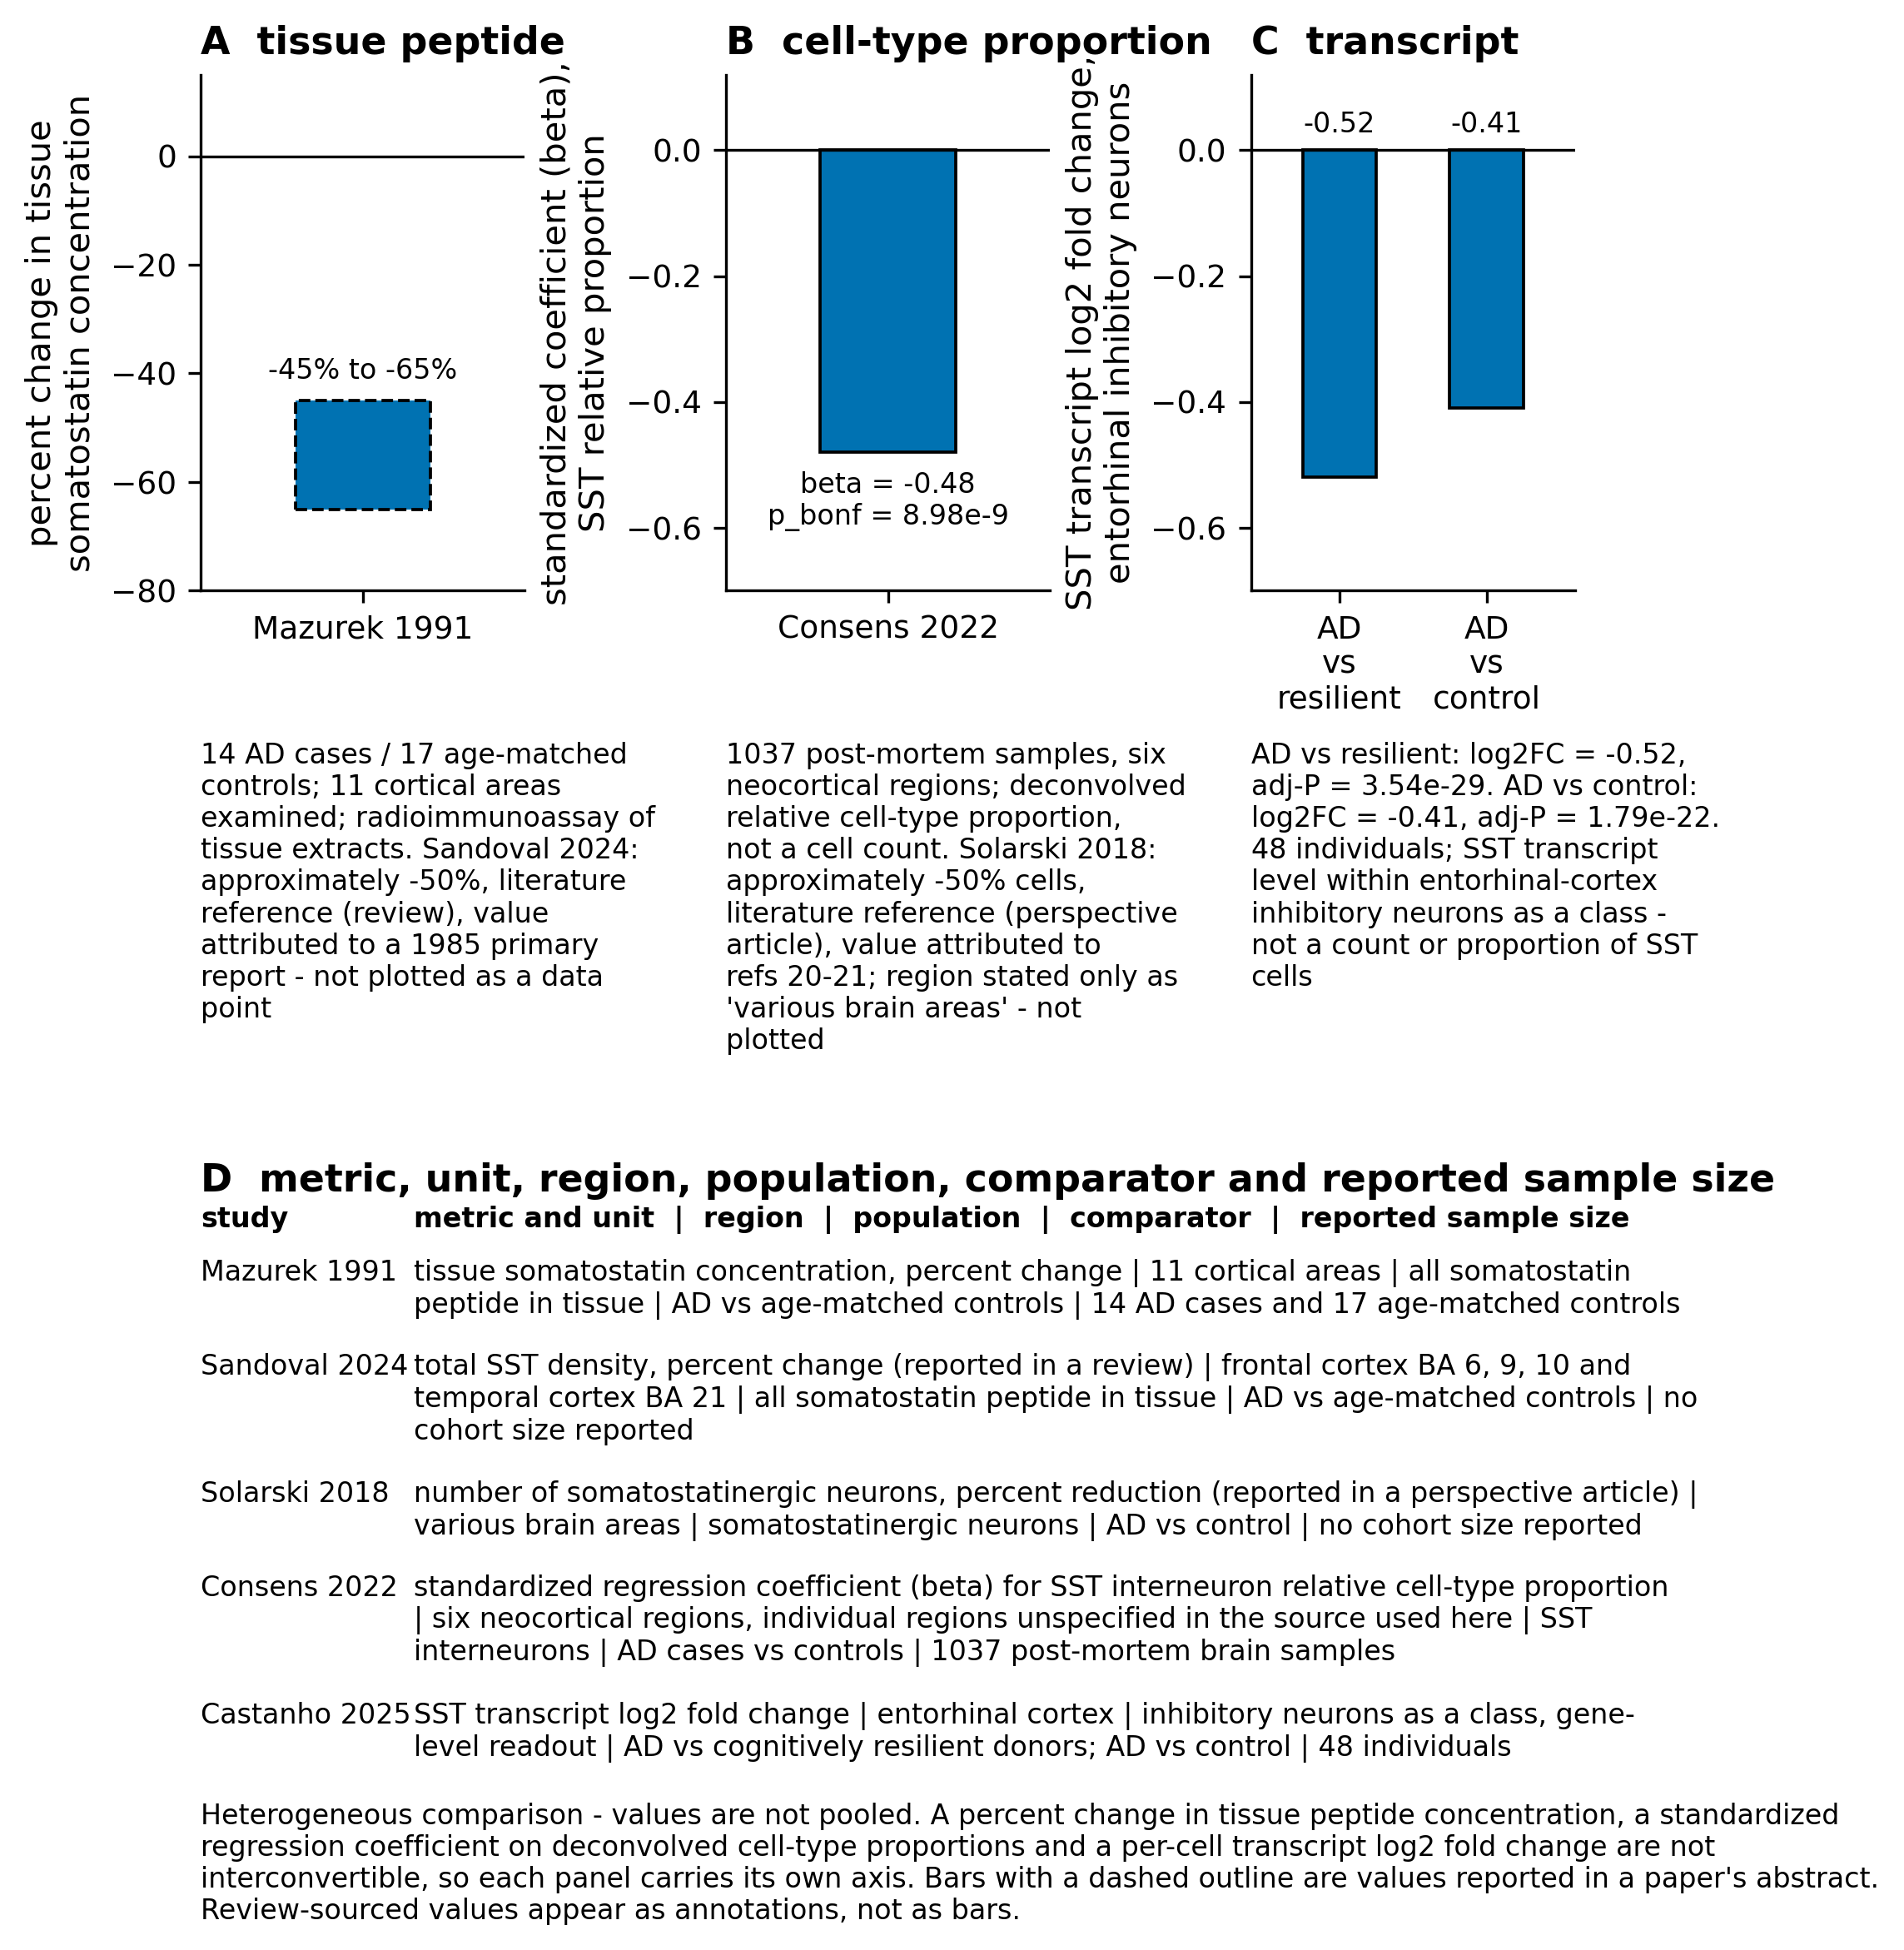
\includegraphics[width=\linewidth]{../figures/fig_sec4_deficit_magnitude_scales.png}
\caption{\textbf{Three assay families, three axes.} The cortical somatostatin deficit in AD reported on the three scales that actually measured it, each on its own axis: percent change in tissue somatostatin concentration (A), the standardized regression coefficient for SST interneuron relative cell-type proportion (B), and \emph{SST} transcript log2 fold change in entorhinal-cortex inhibitory neurons (C), with the metric, unit, region, population, comparator and reported sample size for every entry tabulated in (D). Values are not interconvertible --- a percent change in tissue peptide concentration, a standardized regression coefficient on deconvolved cell-type proportions, and a per-cell transcript log2 fold change --- so each panel has its own axis and no cross-panel comparison of magnitude is implied. \citet{Mazurek1991} reports a range, not a point: somatostatin concentrations were decreased by 45 to 65\% across the cortical areas examined; the bar shows that range, and the source reports no single value. \citet{Solarski2018}'s approximately 50\% is a reduction in the number of somatostatinergic neurons, not a peptide concentration; it is not the same quantity as the peptide reduction in (A), and peptide loss does not imply cell loss because a surviving neuron can downregulate the peptide. \citet{Sandoval2024} and \citet{Solarski2018} are review syntheses reporting values attributed to primary sources --- a 1985 report in the first case, refs 20--21 in the second --- not independent measurements, and are shown as annotations rather than plotted points. \citet{Castanho2025b} measures \emph{SST} transcript level within entorhinal-cortex inhibitory neurons as a class; it is not a count or proportion of SST cells, and both contrasts the study reports are plotted: AD versus cognitively resilient donors (log2FC = $-$0.52) and AD versus control (log2FC = $-$0.41). \citet{Consens2022b} sampled six neocortical regions, named in that study as dorsolateral prefrontal cortex, temporal cortex and Brodmann areas 10, 44, 36 and 22. Reported sample sizes differ in kind: 14 AD cases and 17 controls \citep{Mazurek1991}, 1037 postmortem samples from six neocortical regions \citep{Consens2022b}, 48 individuals \citep{Castanho2025b}. Heterogeneous comparison --- values are not pooled, and no summary estimate is shown. Markers drawn with a dashed edge denote values reported in a paper's abstract.}
\label{fig-sec4-deficit-magnitude-scales}
\end{figure}

\begin{figure}[H]
\centering
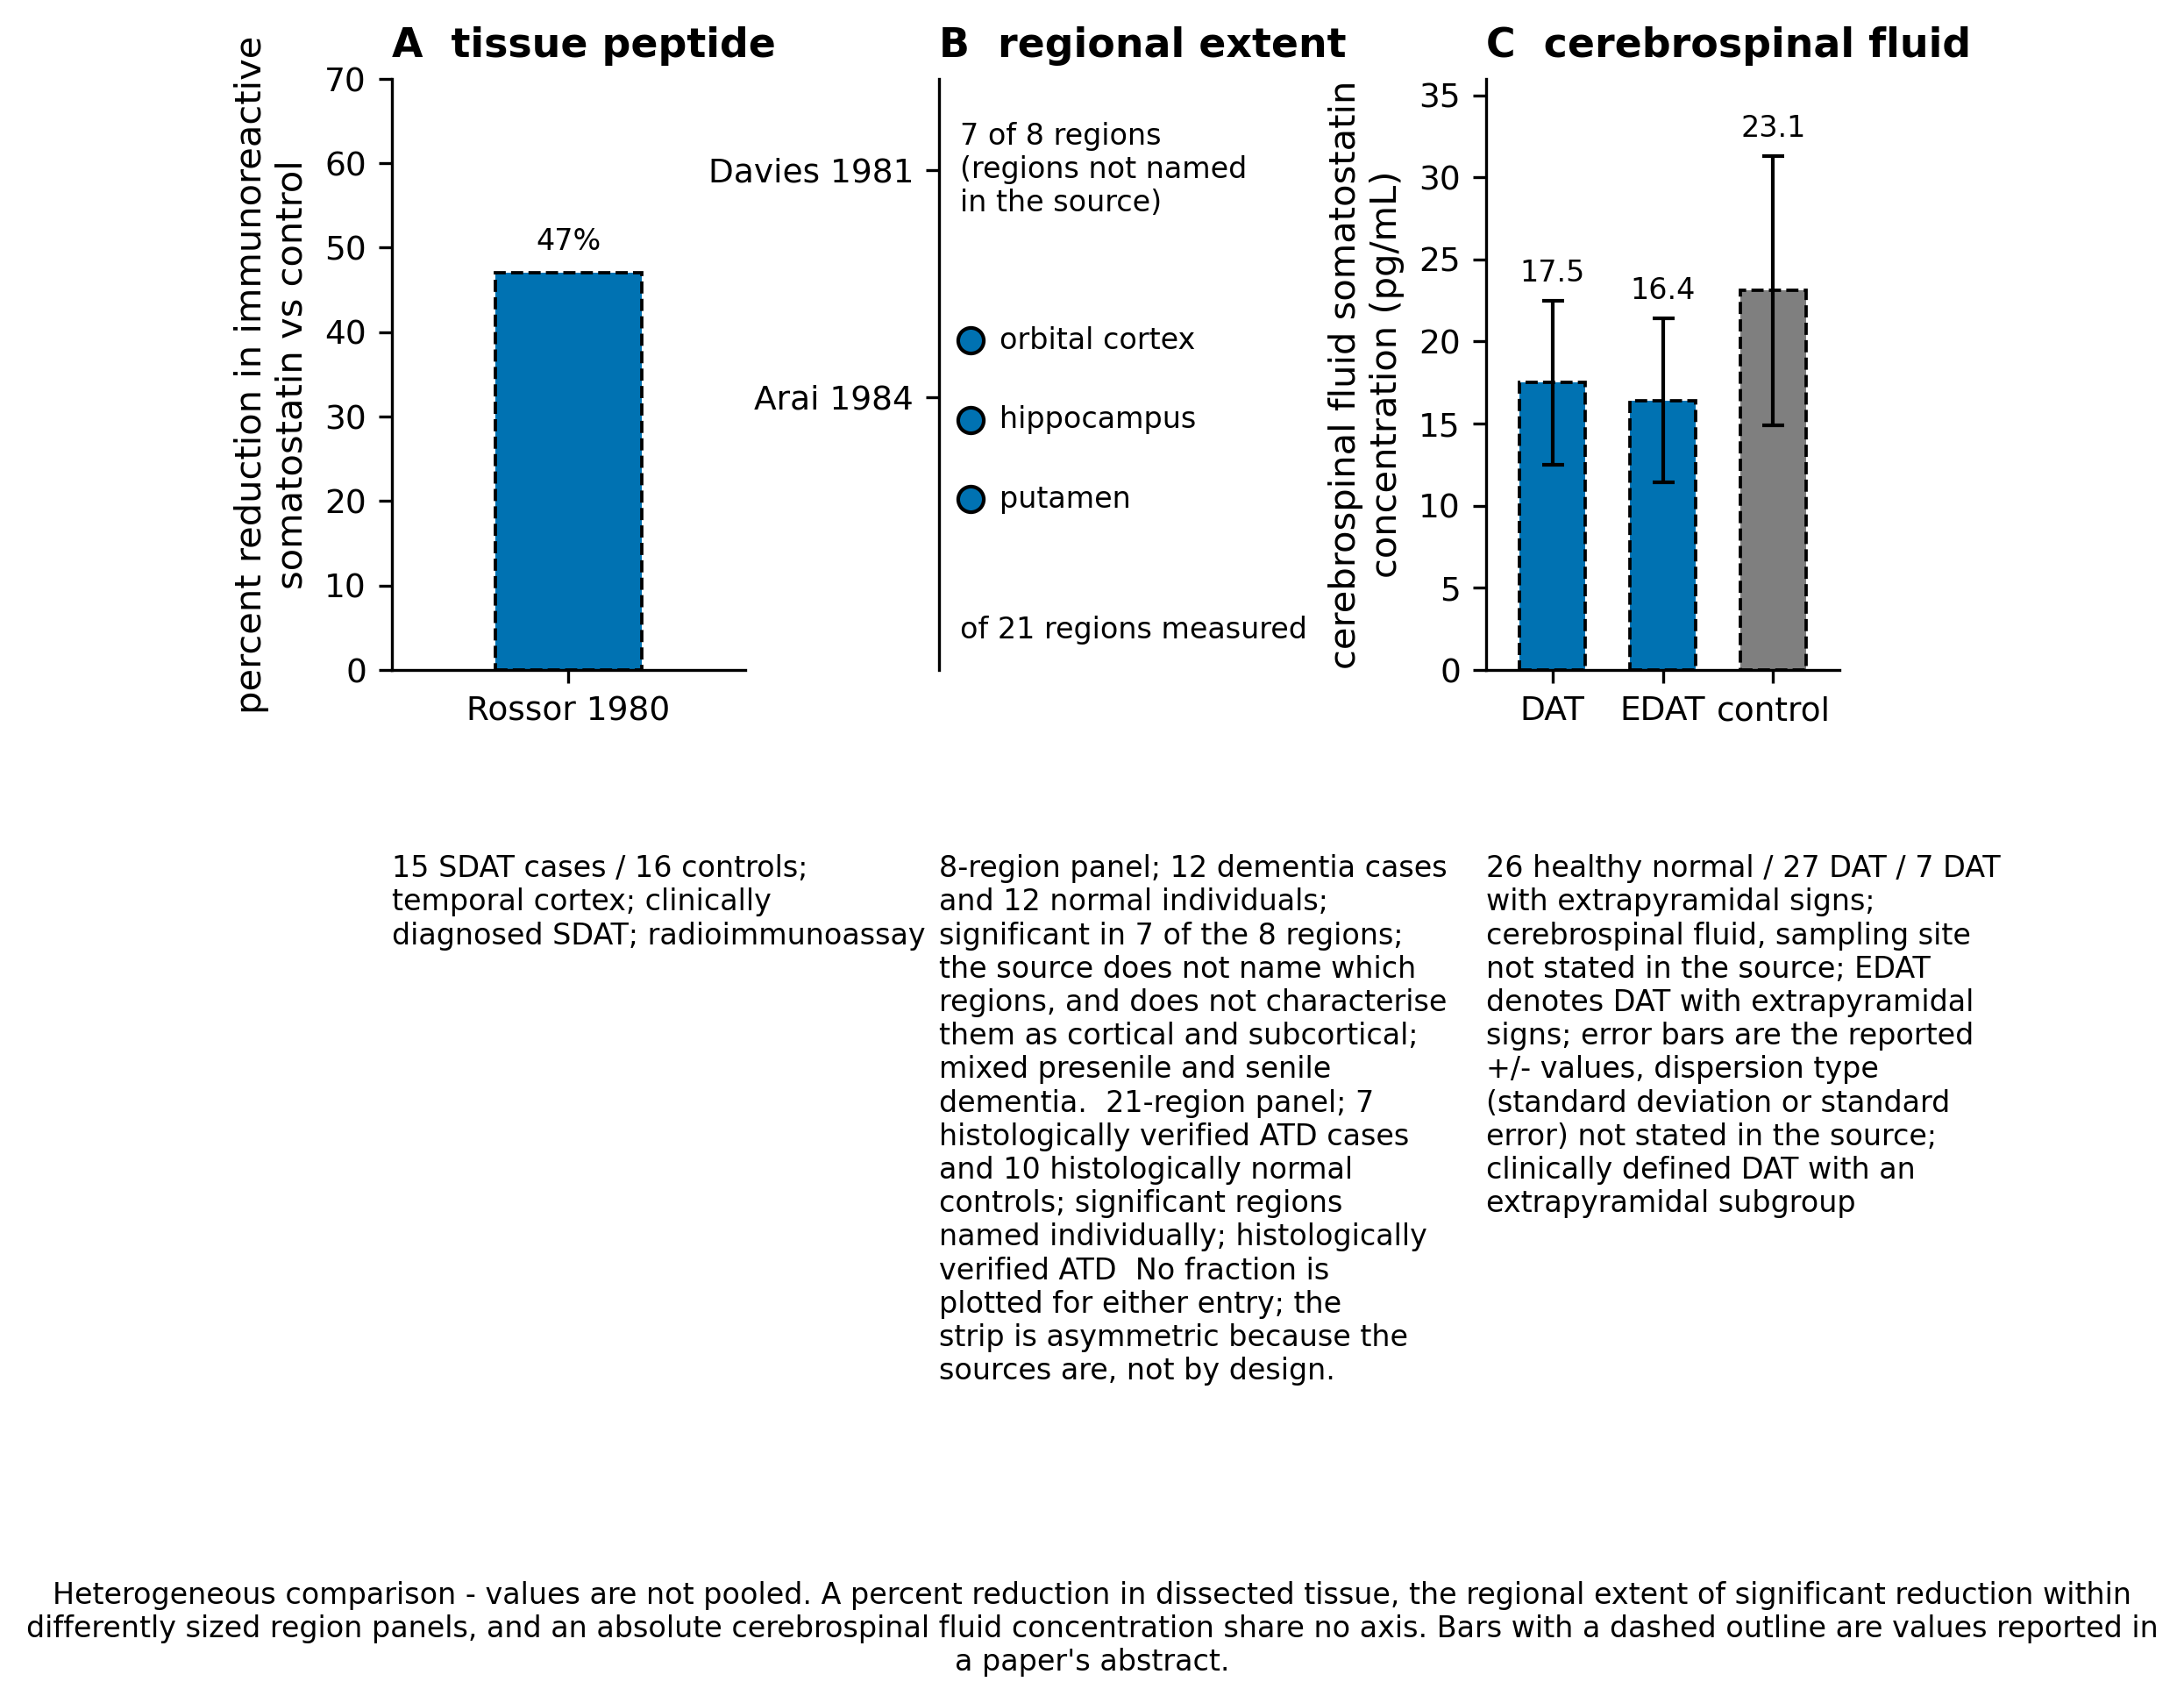
\includegraphics[width=\linewidth]{../figures/fig_sec4_classic_postmortem_csf.png}
\caption{\textbf{The 1980--1988 series, by measurement type.} The classic postmortem and cerebrospinal fluid somatostatin results in AD, separated by what each study measured: percent reduction in immunoreactive somatostatin in temporal cortex (A), the regional extent of significant SLI reduction within differently sized region panels (B), and cerebrospinal fluid somatostatin concentration in pg/mL (C). The metrics are not commensurate and share no axis; in particular a CSF concentration and a tissue percent reduction are not the same construct of somatostatin loss. \citet{Rossor1980} compared 15 SDAT cases with 16 controls. \citet{Davies1981} sampled 8 brain regions and reports that SLI was significantly reduced in 7 of the 8, but the source does not characterise the regions as cortical and subcortical and does not name the 7 in which the reduction was significant; \citet{Arai1984} names orbital cortex, hippocampus and putamen out of 21 regions sampled. The two cannot be read as comparable proportions, and no fraction is plotted for either. \citet{Atack1988} values are reported as mean $\pm$ 5.0 (DAT), $\pm$ 5.0 (EDAT) and $\pm$ 8.2 pg/mL (control); the source does not state whether the dispersion is a standard deviation or a standard error, and the error bars are labelled accordingly. \citet{Atack1988} measured cerebrospinal fluid somatostatin and the source does not state the sampling site; EDAT denotes DAT with extrapyramidal signs. Diagnostic criteria differ across the 1980--1988 span and are not interchangeable, and each panel is annotated with its criterion. Heterogeneous comparison --- values are not pooled. Markers drawn with a dashed edge denote values reported in a paper's abstract.}
\label{fig-sec4-classic-postmortem-csf}
\end{figure}

\subsection{Vulnerable or resilient? The same data type, opposite conclusions}
\label{sec-04-vulnerable-or-resilient}

Two human transcriptomic studies of similar design reach opposite conclusions about the same cell class, and the comparator group is doing most of the work. \citet{Consens2022b} deconvolved bulk and single-nucleus cortical data against unselected non-AD controls and reported SST interneuron proportions as the cell type most reduced in AD, with the reduction tracking plaque burden and cognitive decline. \citet{Castanho2025b} sequenced entorhinal cortex and dorsolateral prefrontal cortex nuclei from 48 individuals spanning AD, cognitively resilient and control donors, and described inhibitory neurons overall as carrying resistance-associated expression profiles, with SST-positive inhibitory subtypes enriched for protective-variant expression --- while simultaneously reporting \emph{SST} transcript itself as one of the most significantly downregulated genes in AD entorhinal inhibitory neurons \citep{Castanho2025a}. The two results are not arithmetically incompatible: a population can be transcriptionally preserved relative to donors matched for pathology and still carry less \emph{SST} message per cell than a control. They are incompatible as summaries, and the peptidomic finding that somatostatin-derived proteoforms are more abundant in resilient than demented AD cortex sits on the resilience side of that line \citep{Morgan2024b}. No study reconciling the two using the same donors, annotation and comparator group was retrieved by these searches; the single-nucleus cohorts that could adjudicate it are examined in \ref{sec-human-evidence}.

\begin{quote}
\noindent\textbf{Evidence Conflict}\par
\textbf{Most depleted cell type, or selectively preserved population? (unresolved).} \citet{Consens2022b} reports SST interneuron relative proportions as the strongest AD-associated cell-type reduction in a mega-analysis of postmortem cortex; \citet{Castanho2025b} describes SST-positive inhibitory neurons as selectively preserved and protective in a resilience-focused single-nucleus cohort. The recorded dimension of disagreement is design and statistical unit --- deconvolved relative proportions across 1037 bulk samples versus per-nucleus differential expression in 48 individuals --- compounded by comparator group (AD versus unselected controls, versus AD versus cognitively resilient donors at matched pathology). Both conclusions are currently drawn from similar human data types, which is why no quantitative statement about the magnitude of SST interneuron loss in AD is defensible.

\end{quote}

The animal-model literature adds a regional disagreement with the same structure. \citet{SanchezMejias2019} counted somatostatin-immunoreactive neurons in perirhinal cortex of APP/PS1 mice and found a decrease of 55.99 $\pm$ 9.13\% and 57.28 $\pm$ 10.96\% in the deep layers of areas 36 and 35 at 6 months relative to 4 months, with the transgenic-versus-control contrast at 6 months reported as a dramatic decrease of 57\% and 61\% in the same two areas. \citet{Ren2025}, tracing long-range inputs to prefrontal interneurons in an AD model at 9 months, found the number of Cre-reporter-labelled SOM-positive neurons in prelimbic cortex not reduced while PV-positive neurons decreased by 16.67\%. \citet{Albuquerque2015} reported a significant decrease of SOM-immunoreactive cells in TgCRND8 hippocampus overall (p = 0.049) and in CA1/2 (p = 0.040) without an effect magnitude. The populations counted are not the same quantity: immunoreactivity can be lost through peptide downregulation in a surviving neuron while a Cre-driven reporter persists, so a reporter-labelled null does not refute an immunoreactivity loss. That caveat is this review's own methodological argument; the two studies supply only the measurements being compared, an immunoreactivity-based human count \citep{GonzalezRodriguez2021} and a Cre-reporter-based mouse count \citep{Ren2025}. Model construct compounds this further: in hAPP transgenic hippocampus, at least 25\% and up to 76\% of somatostatin-expressing neurons across layers themselves express the hAPP transgene, so interneuron phenotypes in those lines are partly cell-autonomous rather than purely a response to extrinsic amyloid \citep{Hofling2019}. The construct-and-dosage explanation for divergent amyloid-model phenotypes is developed in \ref{sec-conflicts-limitations}.

\begin{quote}
\noindent\textbf{Evidence Conflict}\par
\textbf{Regional selectivity of SOM neuron decline in amyloid models (unresolved).} \citet{SanchezMejias2019} reports a decline of more than half in SOM-positive neurons in deep perirhinal layers of APP/PS1 mice between 4 and 6 months; \citet{Ren2025} finds no reduction in SOM-positive neuron number in prelimbic prefrontal cortex of 9-month-old AD model mice, where only PV-positive neurons decline. Whether this is regional selectivity or a general SST vulnerability cannot be settled from these two designs, which differ in model construct, age, region and labelling method.

\end{quote}

What is not in dispute is that SST cells sit inside the amyloid microenvironment. Intracellular A$\beta$ accumulates progressively in SST- and CCK-expressing interneurons of \emph{App} NL-F/NL-F hippocampus (somatic colocalisation 13 $\pm$ 4.0\% for SST cells and 9 $\pm$ 3.7\% for CCK cells) while calretinin cells are comparatively spared \citep{Shi2019}, multi-region spatial transcriptomics finds \emph{Sst} among the GABAergic types significantly enriched within plaque spots across four regions \citep{Bayaraa2025}, and region-resolved interneuron transcriptomics in 5XFAD mice selects the top differentially expressed genes in CA1 \emph{Sst}-positive interneurons for validation, which the authors interpret as mirroring pathway alterations seen in human AD \citep{Chen2025a}. Candidate cell-intrinsic causes of that exposure sensitivity have been proposed --- endoplasmic-reticulum stress generated by processing of the somatostatin precursor itself, with reduced \emph{Perk} lowering ER stress markers in prefrontal SST neurons --- shown in a chronic psychosocial-stress model with n = 4 per genotype, treatment and sex, and with no amyloid manipulation \citep{Tomoda2022} --- and a major AD risk factor remodels the same population's inputs, since a few hours of sleep disruption alters SST interneuron dendritic spine density and spine size in a subregion-specific manner across hippocampus and neocortex \citep{Raven2025}. \ref{fig-sec4-sst-cell-change-regions} assembles the human and model cell-count results with the human and mouse measurements kept in separate panels.

\begin{figure}[H]
\centering
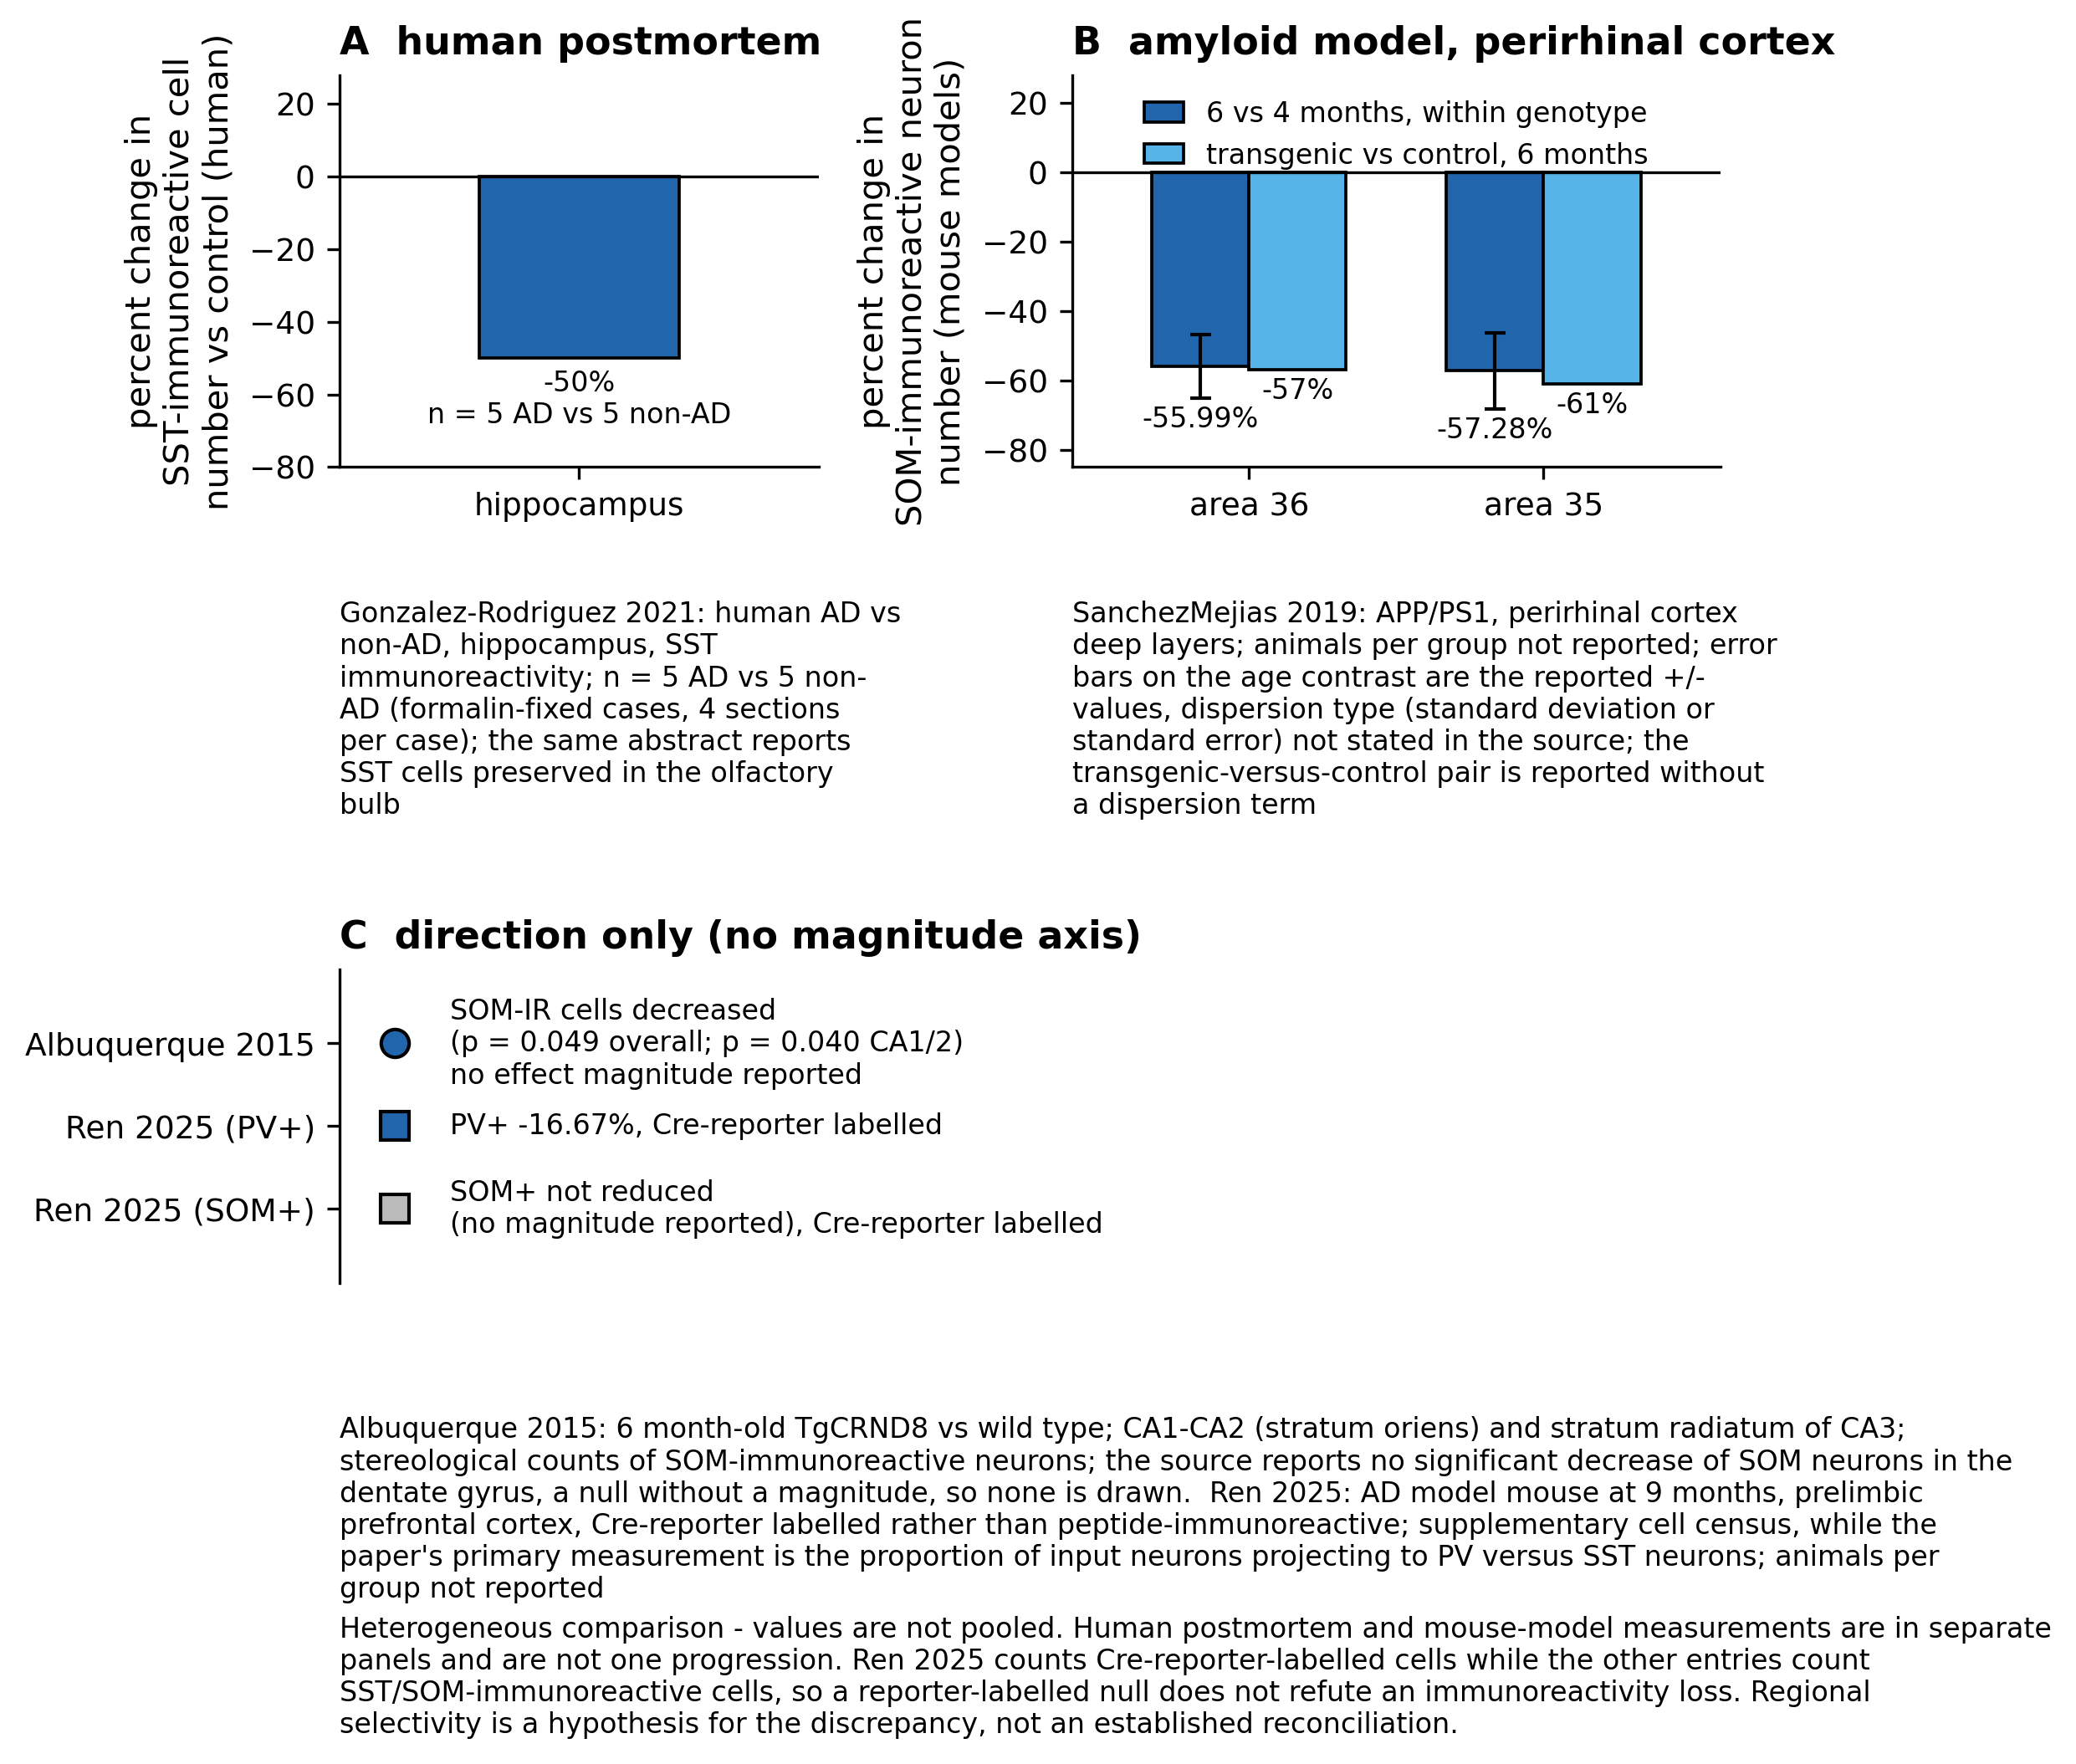
\includegraphics[width=\linewidth]{../figures/fig_sec4_sst_cell_change_regions.png}
\caption{\textbf{Cell counts, by species and region.} Change in SST/SOM cell number in AD and in amyloid mouse models, with human postmortem counts (A) and mouse-model counts (B) on separate percent axes and entries that report no plottable magnitude placed on a direction-only strip (C) rather than on the percent axis. Human postmortem and mouse-model measurements are shown in separate panels and must not be read as one progression; \citet{SanchezMejias2019} itself notes that amyloidogenic models fail to fully recapitulate the selective neuronal degeneration seen in humans. \citet{SanchezMejias2019} contributes two different contrasts to (B): 55.99\% and 57.28\% are 6-month versus 4-month APP/PS1 within genotype, 57\% and 61\% are transgenic versus control at 6 months; both are decreases, are drawn with the same sign, and the comparator is printed on each bar. The error bars on the within-genotype pair are the reported $\pm$ 9.13\% and $\pm$ 10.96\%; the source does not state whether the dispersion is a standard deviation or a standard error, and the transgenic-versus-control pair is reported without a dispersion term. \citet{GonzalezRodriguez2021} quantified cells in 5 AD and 5 non-AD formalin-fixed cases, four sections per case, and the bar prints that cohort. \citet{Albuquerque2015} reports a significant overall decrease in SOM-immunoreactive cells (p = 0.049) and in CA1/2 (p = 0.040); the source gives no effect magnitude, and it does report a dentate gyrus result --- no significant decrease of SOM neurons there --- which carries no magnitude and so is not plotted. The $-$16.67\% on the \citet{Ren2025} marker is the PV-positive value; the SOM-positive result in that study is "not reduced" with no magnitude reported, the cells are Cre-reporter labelled rather than peptide-immunoreactive, and the counts are a supplementary cell census while the paper's primary measurement is the proportion of input neurons projecting to PV versus SST neurons. Because \citet{Ren2025} counts Cre-reporter-labelled SOM-positive neurons while the other entries count SST/SOM-immunoreactive cells, a reporter-labelled null does not refute an immunoreactivity loss. The prefrontal null in \citet{Ren2025} and the olfactory-bulb sparing in \citet{GonzalezRodriguez2021} are observations in different species and regions; regional selectivity is a hypothesis for the discrepancy, not an established reconciliation. Heterogeneous comparison --- values are not pooled.}
\label{fig-sec4-sst-cell-change-regions}
\end{figure}

\subsection{The somatostatin-neprilysin-amyloid axis and its direct refutation}
\label{sec-04-neprilysin-axis}

The mechanistic hypothesis that makes the somatostatin deficit more than a correlate runs in three steps. Step one: somatostatin positively regulates neprilysin activity in neurons, and genetic somatostatin deficiency alters hippocampal neprilysin activity and localisation while raising A$\beta$42 in a manner the authors compared to presenilin mutations \citep{Saito2005}. Step two: neprilysin is transcriptionally enriched in the GABAergic compartment --- among 480 protease and peptidase genes, \emph{Mme} encoding neprilysin is one of only four enriched in cortical interneurons \citep{Rossier2014}, which locates the transcript rather than measuring where enzyme activity resides --- and endothelin-converting enzyme-2, a second major A$\beta$-degrading enzyme, is majorly expressed by somatostatin interneurons and active in isolated synaptosomes \citep{PachecoQuinto2016}. Step three: neprilysin carries a large share of brain A$\beta$ catabolism, since deleting \emph{Mme} in \emph{App} knock-in mice more than doubles GuHCl-soluble A$\beta$40 and A$\beta$42, and combined neprilysin/insulin-degrading-enzyme (IDE) deficiency raises TS-soluble A$\beta$ more than eight-fold, in a fraction the authors note accounts for only 1--5\% of total A$\beta$42 \citep{Morito2025}, with the side-by-side knockout comparison assigning insoluble amyloidogenic A$\beta$ to neprilysin and soluble A$\beta$ to IDE \citep{Sasaguri2021}. A post-transcriptional route into the same node has been described, with microRNA-181d-5p repressing neprilysin 3$'$-UTR activity, mRNA, protein and enzymatic activity while raising tau \citep{Wang2026}. That cellular assignment is contradicted within the same body of work: the knockout comparison that separates insoluble from soluble A$\beta$ attributes neprilysin to secretory vesicles and the presynaptic membranes of excitatory neurons, with neuropeptides secreted from inhibitory neurons instead, and reports that neprilysin deficiency had no significant impact on somatostatin, substance P, cholecystokinin or neuropeptide Y levels \citep{Sasaguri2021}. The chain is therefore coherent as a pathway while its cellular premise remains unsettled: whether the cortex's principal A$\beta$-degrading capacity sits inside the very interneurons whose peptide is depleted depends on which of these localisation results holds.

The receptor arm supplies the strongest positive evidence and also the therapeutic rationale. Loss of SSTR1 and SSTR4 together lowers presynaptic neprilysin and raises hippocampal A$\beta$42 in \emph{App} knock-in mice, with single \emph{Sstr1} or \emph{Sstr4} knockouts leaving A$\beta$ unaltered, and an SSTR1/SSTR4-selective agonist robustly increasing hippocampal neprilysin expression alongside a clear reduction in plaque load relative to the contralateral side \citep{Nilsson2020,Nilsson2025}. These two reports carry the same SSTR1/SSTR4-neprilysin result and one of them carries a preprint identifier; whether they are two independent tests or one programme reported twice cannot be determined from the retrieved record, so the receptor arm may rest on fewer experiments than the citation count suggests. Downstream of the receptor, somatostatin control of neprilysin has been placed on a SUR1/Kir6.2 pathway --- \emph{Abcc8} knockout significantly decreased hippocampal neprilysin activity with a significant increase of both A$\beta$40 and A$\beta$42 \citep{Watamura2021} --- and $\alpha$-endosulfine has been identified as a negative regulator acting downstream, its genetic loss enhancing neprilysin activity and decreasing A$\beta$ deposition \citep{Watamura2020}. Pharmacological agonism reproduces the transcript signature: the SSTR4 agonist NNC 26-9100 increased cortical expression of \emph{Sstr4} 4.9-fold, neprilysin 9.3-fold, insulin-degrading enzyme 14.8-fold and catalase 3.6-fold at 24 h \citep{Sandoval2019}, and improved learning while lowering soluble A$\beta$42 oligomers through a phosphoramidon-sensitive metalloproteinase mechanism \citep{Sandoval2013}. A different SSTR4 agonist, L-803087, applied to differentiated SH-SY5Y cells raised Ser522-CRMP2 phosphorylation in a concentration-dependent manner, alone and in combination with A$\beta$1--42; in that study the protective arm is somatostatin-mediated inhibition of Ser522-CRMP2 phosphorylation, and the agonist-driven increase is read as a consequence of receptor internalisation rather than as the means by which A$\beta$ cytotoxicity is counteracted \citep{Paik2021}. Brain-penetrant protein engineering targets the same enzyme from the other side: a somatostatin fusion protein raised hippocampal neprilysin levels, with the membrane-fraction increase correlating with the fall in A$\beta$42 \citep{Rofo2021}, a somatostatin-based therapeutic that activates neprilysin reduced both oligomeric and larger A$\beta$ aggregates \citep{Metzendorf2025}, directed evolution produced a neprilysin variant with 20-fold increased catalytic efficiency on A$\beta$1--40 and up to 3.2 $\times$ 10$^{3}$-fold reduced cleavage of off-target peptides \citep{Webster2014}, and a blood--brain-barrier-penetrating fusion construct showed A$\beta$40 degradation that depended strongly on the A$\beta$-to-enzyme ratio \citep{Rofo2022}. Reciprocally, intracortical A$\beta$25--35 lowers both somatostatin and neprilysin expression in rat temporal cortex, and minocycline prevents both reductions \citep{BurgosRamos2009}.

Against that coherence stands one in vivo test on an amyloidosis background, and it is negative on the mechanism. Crossing \emph{Sst}-null mice to the \emph{App} NL-F/NL-F knock-in, \citet{Williams2023} found that neither whole-brain neprilysin transcript nor protein nor activity levels were affected by \emph{Sst} genotype, yet \emph{Sst} ablation still produced significantly stronger cortical A$\beta$ deposition at 15 months; cortical plaque density rose 3.7-fold, 4.6-fold and 4.5-fold between 12 and 15 months in the three \emph{Sst} genotypes, and the paralog \emph{Cort} increased by approximately 35\% in \emph{Sst}-deficient mice without preventing the plaque increase, in the journal and preprint reports of that one cross \citep{Williams2023,Williams2022}. The authors' interpretation is that endogenous somatostatin slows deposition by interfering with A$\beta$ aggregation directly rather than by inducing neprilysin, and there is independent biophysical support for a direct interaction: somatostatin-14 binds selectively to the $\beta$-barrel pore-forming A$\beta$(1--42) tetramer with a KD of approximately 40 $\mu$M and 2:1 stoichiometry without binding monomeric A$\beta$(1--42) \citep{Puig2020}, elevated somatostatin and A$\beta$ may form mixed oligomeric assemblies with a specific somatostatin residue required for the effect on fibrillization kinetics \citep{Solarski2018}, and the clinical analogues octreotide and lanreotide protected hippocampal cells from A$\beta$42 toxicity (cell viability 83.8\% and 81\%) more effectively than native somatostatin \citep{Pham2025}. A third, non-enzymatic route is also on the table, with somatostatin acting on microglia through SSTR2 to enhance phagocytosis, and somatostatin overexpression reducing microglial density and plaque burden while improving hippocampus-dependent memory \citep{Jung2026}.

\begin{quote}
\noindent\textbf{Evidence Conflict}\par
\textbf{Does somatostatin control brain A$\beta$ through neprilysin? (unresolved; the most consequential disagreement in this review).} \citet{Saito2005} reports that somatostatin selectively upregulates neprilysin activity among tested effectors and that genetic somatostatin deficiency alters hippocampal neprilysin activity and localisation while increasing A$\beta$42. \citet{Williams2023} reports no effect of \emph{Sst} ablation on whole-brain neprilysin transcript, protein or activity in an \emph{App} knock-in background, with cortical plaque density nonetheless significantly increased, and attributes the effect to direct interference with A$\beta$ aggregation. The recorded axis of disagreement is measurement modality and what was counted --- hippocampal enzyme activity in a wild-type-background knockout versus whole-brain transcript, protein and activity in an amyloid knock-in cross. The recorded disagreement in the receptor arm sets \citet{Nilsson2020}, which reports that combined SSTR1/SSTR4 loss lowers presynaptic neprilysin and raises hippocampal A$\beta$42, against \citet{Williams2022}, which reports unchanged brain neprilysin after ligand knockout on the same \emph{App} knock-in background; \citet{Williams2022} is the preprint of \citet{Williams2023}, so this is the same ligand-knockout experiment appearing a second time rather than an additional one. Both sets of results are currently cited as if they agreed. No study measuring neprilysin protein and activity, A$\beta$ species and plaque load side by side in ligand-knockout and SSTR1/SSTR4 receptor-knockout mice on the same \emph{App} knock-in background was retrieved by these searches.

\end{quote}

Two further cautions belong with this axis. First, the claim that neprilysin is regulated by the neuropeptide somatostatin is repeated across primary papers and reviews in this literature, but no original demonstration in human tissue was identified here; all the primary evidence retrieved is rodent or cell culture, and no retrieved human study quantifies neprilysin protein or activity specifically within SST or PV interneurons in AD versus control cortex --- the missing load-bearing experiment, if that degrading capacity is indeed concentrated in the interneurons that lose their peptide. Second, the therapeutic programme described in \ref{sec-therapeutics} --- SSTR4-selective chemistry now reaching thirty-three compounds with sub-100 nM binding affinity, five of them sub-nanomolar with more than 300-fold selectivity over other subtypes \citep{Crider2025}, and structural refinement of SSTR4 agonist contacts \citep{Slater2025} --- inherits the neprilysin premise from this disputed chain, against a negative human precedent: octreotide produced no clinically significant cognitive improvement in Alzheimer dementia and a generalized decrease in glucose metabolism on positron emission tomography in 6 patients \citep{Mouradian1991}. \ref{fig-sec4-neprilysin-axis} sets out the quantities that are actually measured in this axis, and makes clear that they do not form a single causal chain.

\begin{figure}[H]
\centering
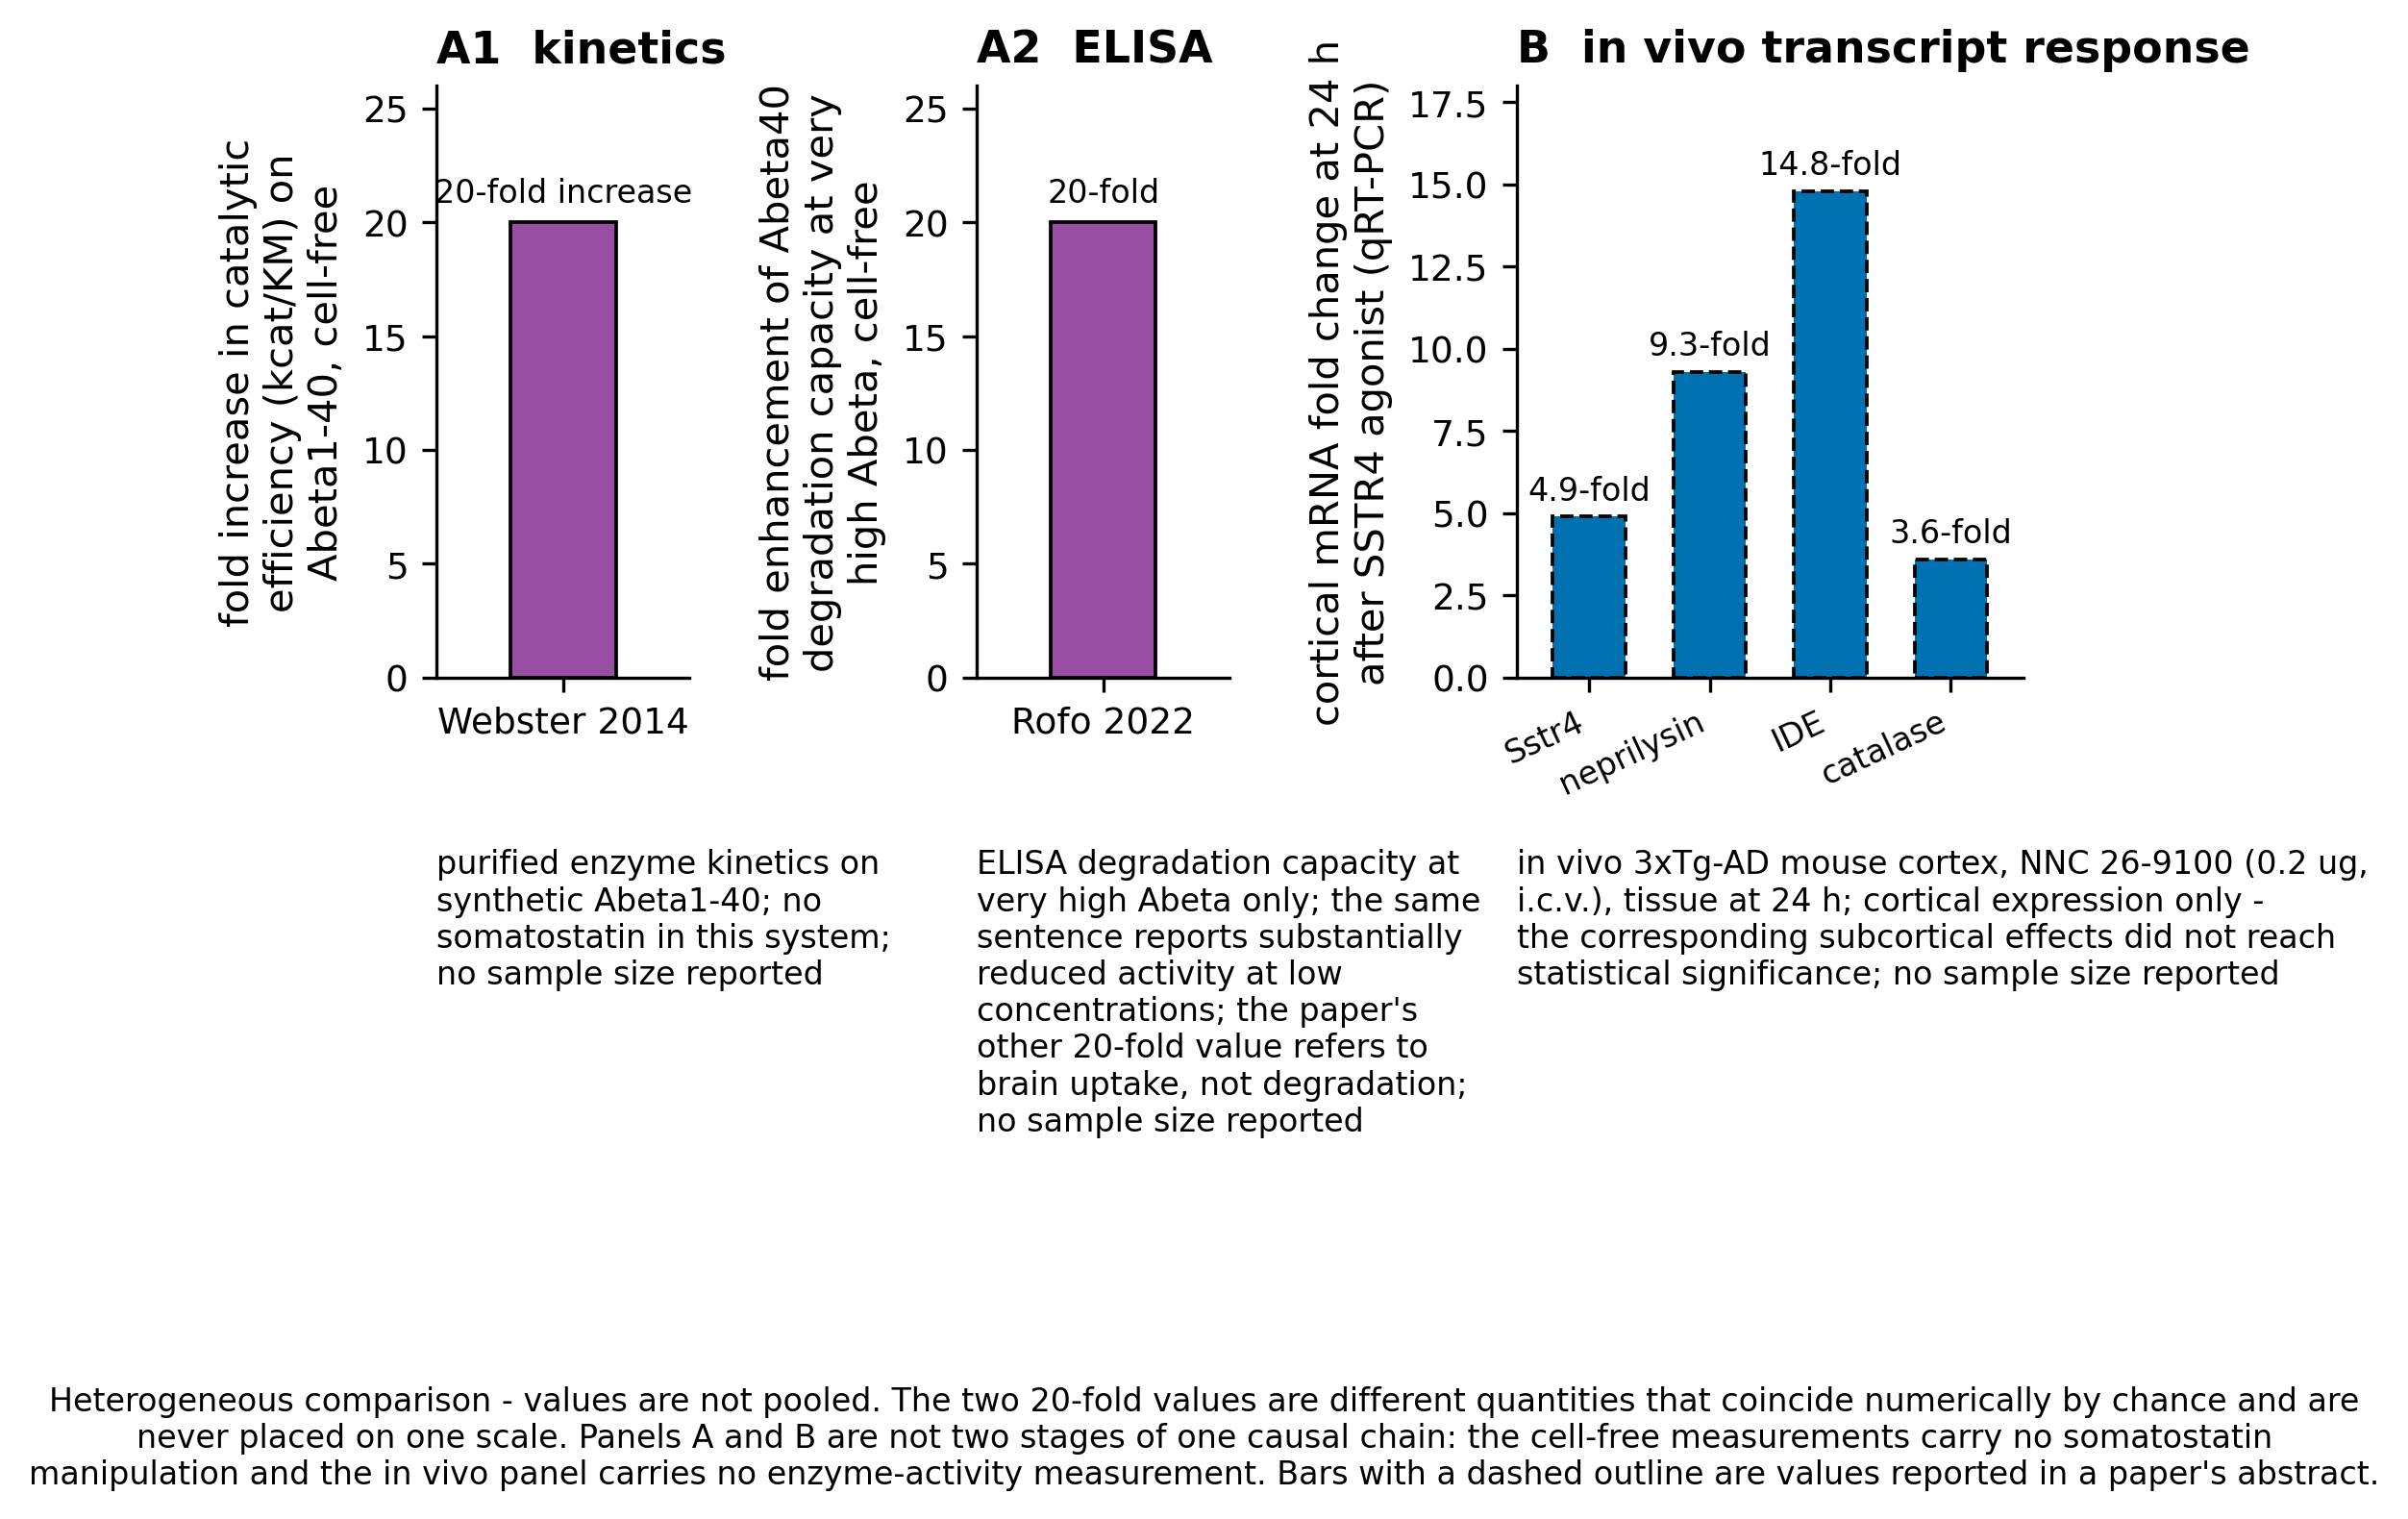
\includegraphics[width=\linewidth]{../figures/fig_sec4_neprilysin_axis.png}
\caption{\textbf{What the neprilysin axis actually measures.} Quantities reported for neprilysin in relation to A$\beta$ and to somatostatin signalling, each on its own axis: cell-free catalytic efficiency (kcat/KM) of an engineered neprilysin variant on A$\beta$1--40 (A1), cell-free ELISA A$\beta$40 degradation capacity at very high A$\beta$ concentration (A2), and cortical mRNA fold change at 24 h after the SSTR4 agonist NNC 26-9100 (B). The two 20-fold values are different quantities --- a cell-free catalytic efficiency ratio \citep{Webster2014} and an ELISA degradation capacity at very high substrate concentration \citep{Rofo2022} --- and coincide numerically by chance; they are plotted on separate axes and never adjacent on one scale. \citet{Rofo2022} itself states that the mutated neprilysin variant was suggested to have higher degradation efficiency of A$\beta$ compared with other neprilysin substrates, but not per se to degrade A$\beta$ more efficiently; the 20-fold figure is an ELISA capacity measured only at very high A$\beta$ concentration, with substantially reduced activity at low concentrations reported in the same sentence, and the same paper's other 20-fold value refers to brain uptake rather than degradation. \citet{Sandoval2019}'s four fold changes are cortical expression at 24 h; the paper reports that the corresponding subcortical effects did not reach statistical significance. Panels A and B are not two stages of one causal chain: the cell-free enzyme measurements were not performed in the presence of brain tissue and carry no somatostatin manipulation, and the in vivo panel carries no direct enzyme-activity measurement. No entry in this figure reports a sample size, so no bar is weighted by cohort size. Heterogeneous comparison --- values are not pooled. Markers drawn with a dashed edge denote values reported in a paper's abstract.}
\label{fig-sec4-neprilysin-axis}
\end{figure}

\subsection{Tau, SST interneurons, and cell-class tropism}
\label{sec-04-tau-tropism}

Whether pathological tau preferentially burdens inhibitory neurons is contested along a seeded-versus-spontaneous axis. Inoculating mouse hippocampus with extracellular vesicles from AD brain, \citet{Ruan2020} found that 64\% of AT8-positive cells were GAD67-positive interneurons against 23\% GluR2/3-positive excitatory mossy cells, and that interneurons receiving the transferred tau fired fewer action potentials at +100 pA (P = 0.0434) and +130 pA (P = 0.0445) than those from tau-knockout-vesicle controls. Human postmortem and PS19 transgenic material point the other way on aggregation: \citet{Broekaart2025} reports tau aggregating predominantly in excitatory neurons, while finding inhibitory neurons far more transcriptionally perturbed in vulnerable regions --- 1733 differentially expressed genes in prefrontal inhibitory neurons against 223 in excitatory neurons. Human induced pluripotent stem cell-derived subtypes seeded with sporadic AD brain tau sit with the interneuron-vulnerability side, cortical inhibitory neurons consistently displaying the most MC1-positive insoluble tau aggregation across donor lines \citep{Weidling2025}, whereas a chaperone-based account identifies a tau homeostasis signature in which BAG3 overexpression significantly attenuated tau accumulation in excitatory neurons (P < 0.01) with only a non-significant trend in inhibitory neurons (P = 0.098), attributed to the low level of tau aggregate in inhibitory cells in the first place \citep{Fu2018}. Cross-dataset modelling of regional tau burden recovers excitatory CA1-prosubiculum neuron density as the dominant correlate; \emph{Sst}-positive interneurons correlate positively with tau across datasets while \emph{Pvalb}-positive interneurons show the opposite, and a positive association for both together appears only in the unseeded combined amyloid/tau model \citep{Torok2025}.

\begin{quote}
\noindent\textbf{Evidence Conflict}\par
\textbf{Cell-class tropism of pathological tau (unresolved).} \citet{Ruan2020} finds the majority of AT8-positive cells in inoculated mouse hippocampus to be GAD67-positive interneurons; \citet{Broekaart2025} finds tau accumulation predominantly in excitatory neurons in human cortex and PS19 mice. The recorded axis is species, region and circuit context, confounded by seeded mouse inoculation versus spontaneous human and transgenic pathology, and by region --- hippocampus versus prefrontal cortex. Neither design can be converted into the other, and the disagreement is about which cells carry aggregate, not about whether inhibitory circuits are affected.

\end{quote}

Tau-bearing dystrophic survivors are a phenotype distinct from cell loss, and they were described in the earliest human material: surviving somatostatin neurons are distorted with short dendrites and truncated axons, with loss most severe where tangle and plaque indices are highest \citep{ChanPalay1987}, and cortical somatostatin-immunoreactive perikarya show morphological changes consistent with degeneration \citep{Roberts1985}. The TgF344-AD rat reproduces this directly, with dystrophic SST neurons making up more than 40\% of the hippocampal SST population at 15 months (F(2,6) = 72.61, P < 0.0001) while parvalbumin neuroplasticity compensates \citep{Morrone2022}, against a human pathological background in which phospho-tau-positive neuron density rises from 3.3 $\pm$ 5.8 AT8-positive neurons/mm$^{2}$ in non-demented cases to 14.2 $\pm$ 18.2 in Alzheimer's dementia \citep{MerinoSerrais2025}. Tau also degrades the excitatory drive onto inhibitory cells: in P301S hippocampus, AMPA receptor density falls at synaptic and extrasynaptic sites of both pyramidal cells and interneurons \citep{AlfaroRuiz2022b}, and synaptic NMDA receptors on CA1 interneurons are reduced in a layer-specific pattern while extrasynaptic GluN1 increases in stratum radiatum interneuron dendrites \citep{AlfaroRuiz2022a}. Interneuron subtypes are lost early and progressively in the same line, with aberrantly increased LTP as the functional correlate \citep{Bold2022}, GABA-related gene expression falls in tauopathy prefrontal cortex with epigenetic activation of \emph{Gad1} restoring inhibitory currents and spatial memory \citep{Wan2025}, and positive allosteric modulation of $\alpha$5-GABA-A receptors --- a major postsynaptic target of dendritic inhibition --- mitigated spine loss and reversed working-memory deficits in PS19 mice without altering phospho-tau levels \citep{Dharavath2024}. Tau is not simply permissive for hyperexcitability either: deleting \emph{Mapt} changes the electrographic character of induced epileptogenesis rather than abolishing it, with 10 of 17 (58.82\%) tau-null animals progressing from status epilepticus to spontaneous recurrent seizures against 38 of 42 (90.47\%) wild-type mice \citep{Moseley2025}.

\subsection{Network hyperexcitability: how much is biology and how much is recording time}
\label{sec-04-hyperexcitability}

Any statement about how common epileptiform activity is in AD is a statement about the recording protocol. On overnight video-EEG with magnetoencephalography, subclinical epileptiform activity was detected in 42.4\% of 33 AD patients without a seizure history against 10.5\% of 19 age-matched controls (p = 0.02), and was associated with faster cognitive decline \citep{Vossel2016}. A narrative review reports, from a cited study of 1617 unselected dementia patients on routine short EEG, epileptiform discharges in 42 subjects (3\%), 60\% of whom had no clinical seizures \citep{Chen2024}. Pushing the electrode closer detects activity that scalp recording misses: in two index patients with no clinical or scalp-EEG evidence of epilepsy, foramen ovale recordings revealed clinically silent hippocampal seizures and spikes concentrated during sleep --- a demonstration of detectability rather than a prevalence estimate \citep{Lam2017}. A frequently quoted literature range of 42\%--64\% for overt seizures or subclinical epileptic activity sits inside a mouse tau-model paper rather than a clinical cohort \citep{Gao2026}. Detection criteria are themselves under question: in 30 patients with early-stage AD without a history of epilepsy, questionnaire-positive epilepsy symptoms were more common among patients with any suspicious EEG features (4/7, 57\%) than among those without (4/23, 17\%; p = 0.037) --- a subgroup split within the patient arm, while the cohort-level discharge rate, 3 patients (10\%) against 1 control (3.33\%), did not reach significance (p = 0.612) --- the authors concluding that current morphological criteria may exclude true epileptiform activity in this population \citep{BSzabo2026}. These prevalence estimates come from small, heterogeneous cohorts with different modalities and no shared detection criteria, and should not be pooled into a single figure for how common subclinical seizures are in AD; \ref{fig-sec4-epileptiform-rates} groups them by detection protocol instead.

The surrounding human readouts are equally heterogeneous and equally small, and \ref{fig-sec4-human-hyperexcitability-markers} keeps the two quantified ones on separate axes. Theta--gamma phase-amplitude coupling in left parahippocampal cortex was reduced in AD, with a cohort-level normalized value of $-$0.235 in 50 biomarker-positive patients against 0.312 in 35 cognitively unimpaired controls (P = 0.037) \citep{Prabhu2024}. High-frequency oscillations above 250 Hz and epileptiform discharges are detectable on scalp EEG in Down syndrome with AD, where 57\% (8/14) of participants showed epileptiform activity and HFO-positive channels were regionally distributed by symptomatic status (p = 0.003) \citep{Lisgaras2025}. The inference also runs backwards: 17\% of a prospective cohort with late-onset unexplained epilepsy met criteria for mild cognitive impairment (MCI) within five years of seizure onset \citep{Sarkis2024}. Whether suppressing the activity helps is still unanswered in humans --- a randomized crossover trial of levetiracetam in AD patients who had never had a seizure recruited 8 of a planned 30 participants before being halted, establishing tolerability but not efficacy \citep{Sen2024}. None of these human measurements identifies a cell type; the attribution of human network hyperexcitability to SST or PV interneuron dysfunction rests entirely on mouse models.

\begin{figure}[H]
\centering
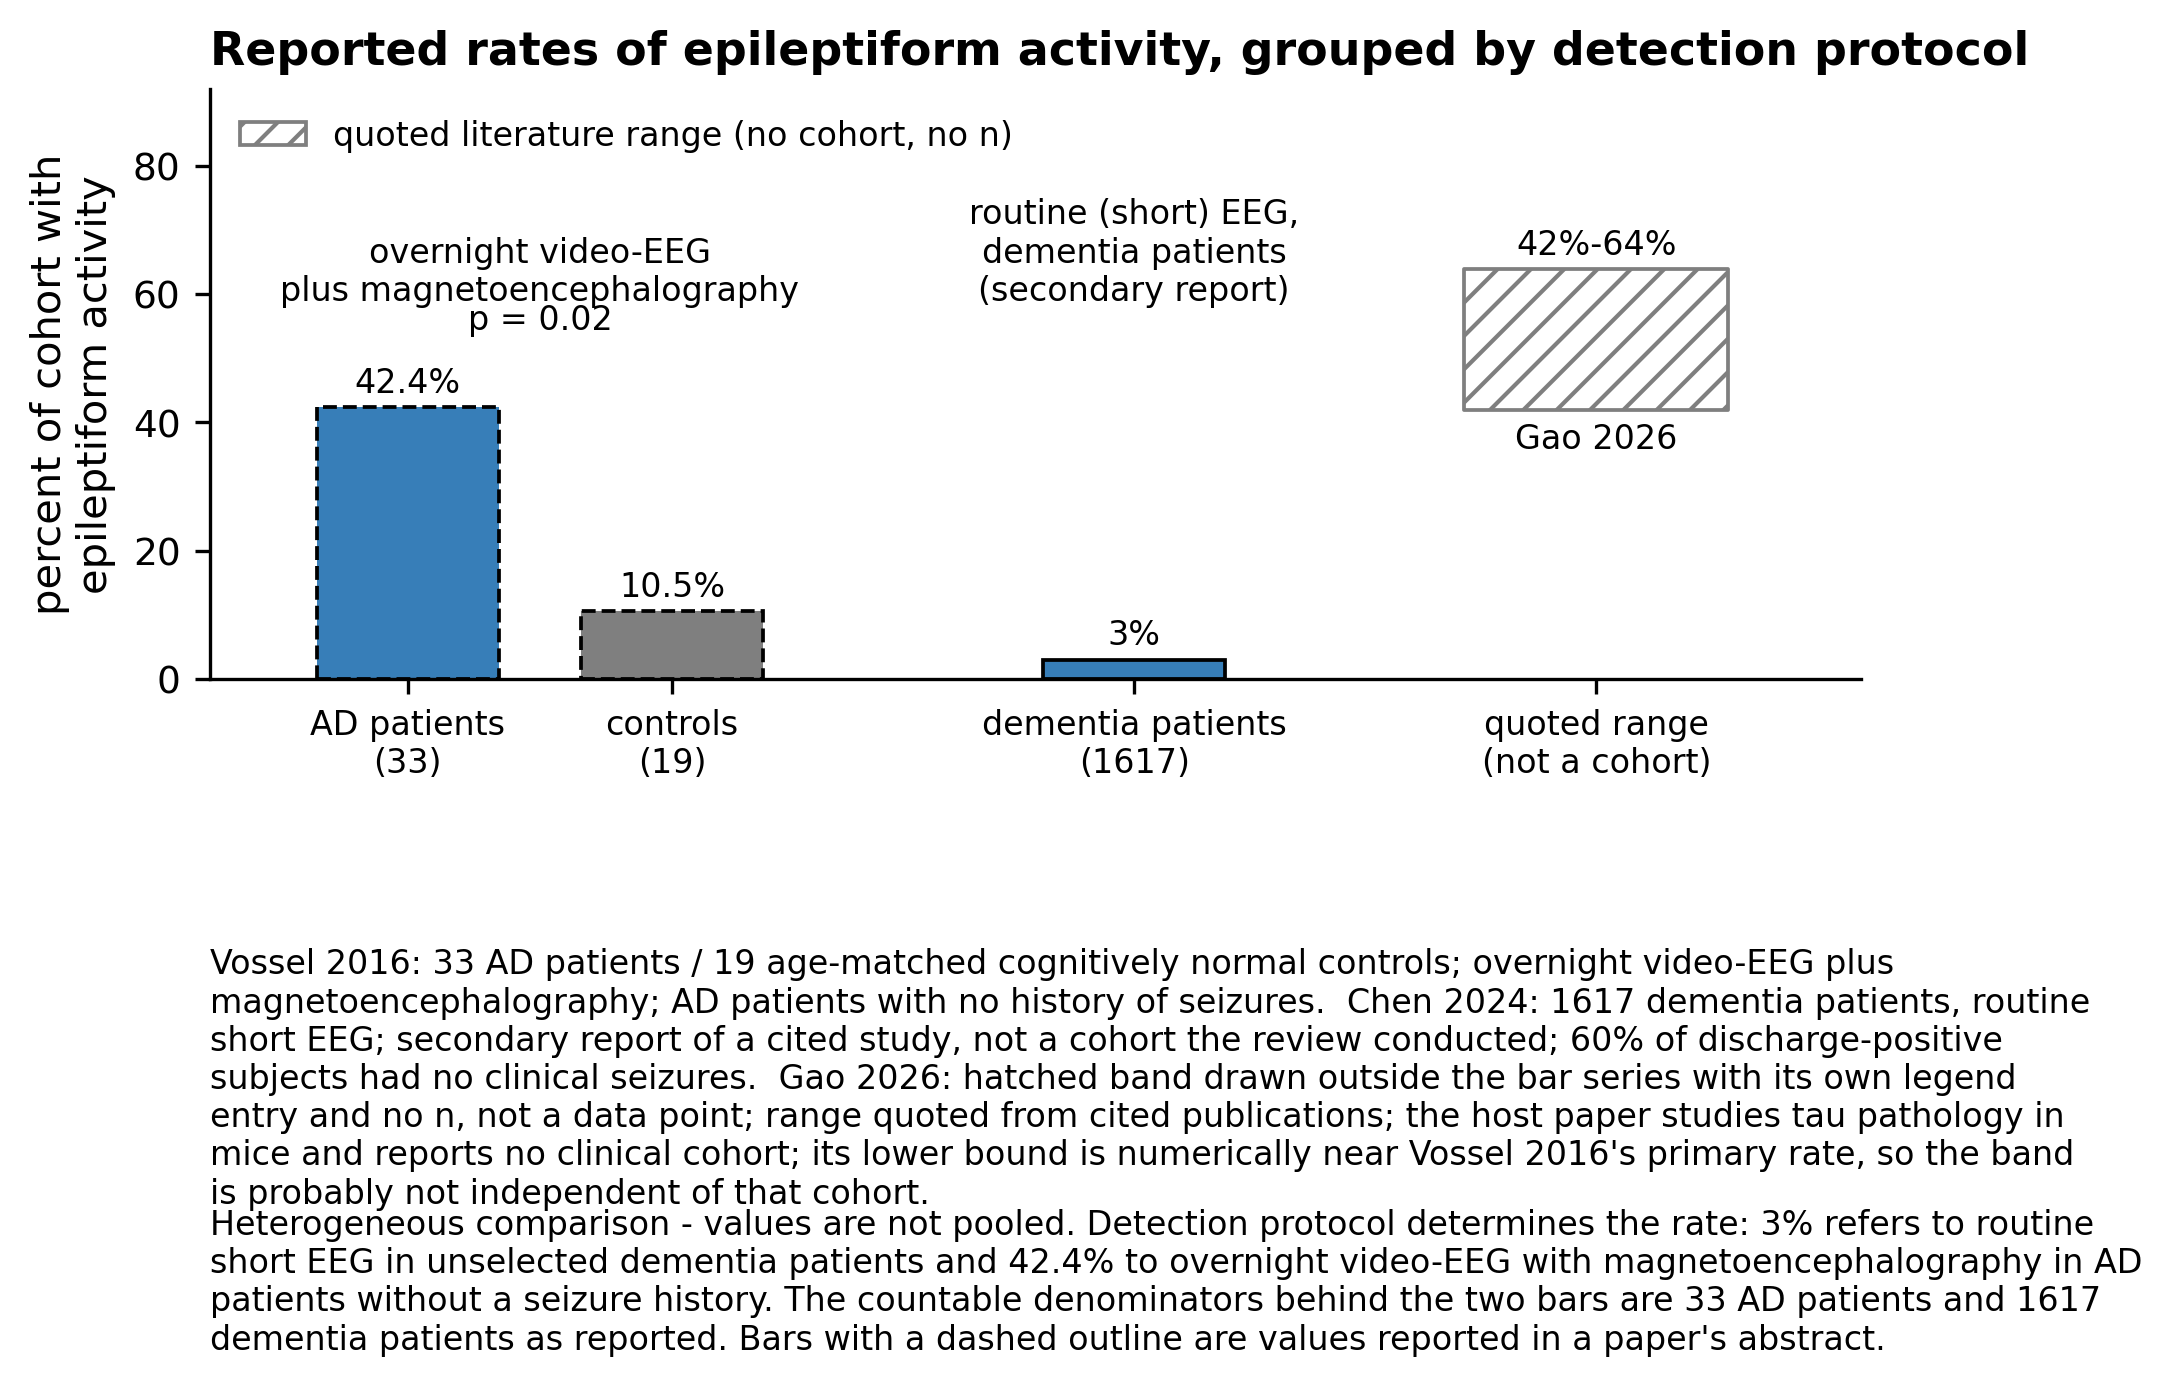
\includegraphics[width=\linewidth]{../figures/fig_sec4_epileptiform_rates.png}
\caption{\textbf{Rate follows protocol.} Reported rates of epileptiform activity in AD and dementia cohorts on a single prevalence axis, with bars grouped and labelled by detection protocol and the reported cohort counts printed on every bar. Detection protocol determines the rate: 3\% refers to routine short EEG in unselected dementia patients, 42.4\% to overnight video-EEG with magnetoencephalography in AD patients without a seizure history. \citet{Chen2024}'s 3\% is a secondary report of a cited study of 1617 unselected dementia patients, not an AD-only cohort. \citet{Vossel2016} enrolled 33 AD patients with no history of seizures and 19 age-matched controls. The countable denominators behind the two bars are therefore 33 AD patients and 1617 dementia patients as reported. \citet{Gao2026}'s 42\%--64\% is a range quoted from cited publications inside a mouse tau-model paper and probably includes the \citet{Vossel2016} cohort; it is drawn as a hatched literature band outside the bar series with its own legend entry, carries no cohort of its own, and is not independent corroboration of the bars. Heterogeneous comparison --- values are not pooled. Markers drawn with a dashed edge denote values reported in a paper's abstract.}
\label{fig-sec4-epileptiform-rates}
\end{figure}

\begin{figure}[H]
\centering
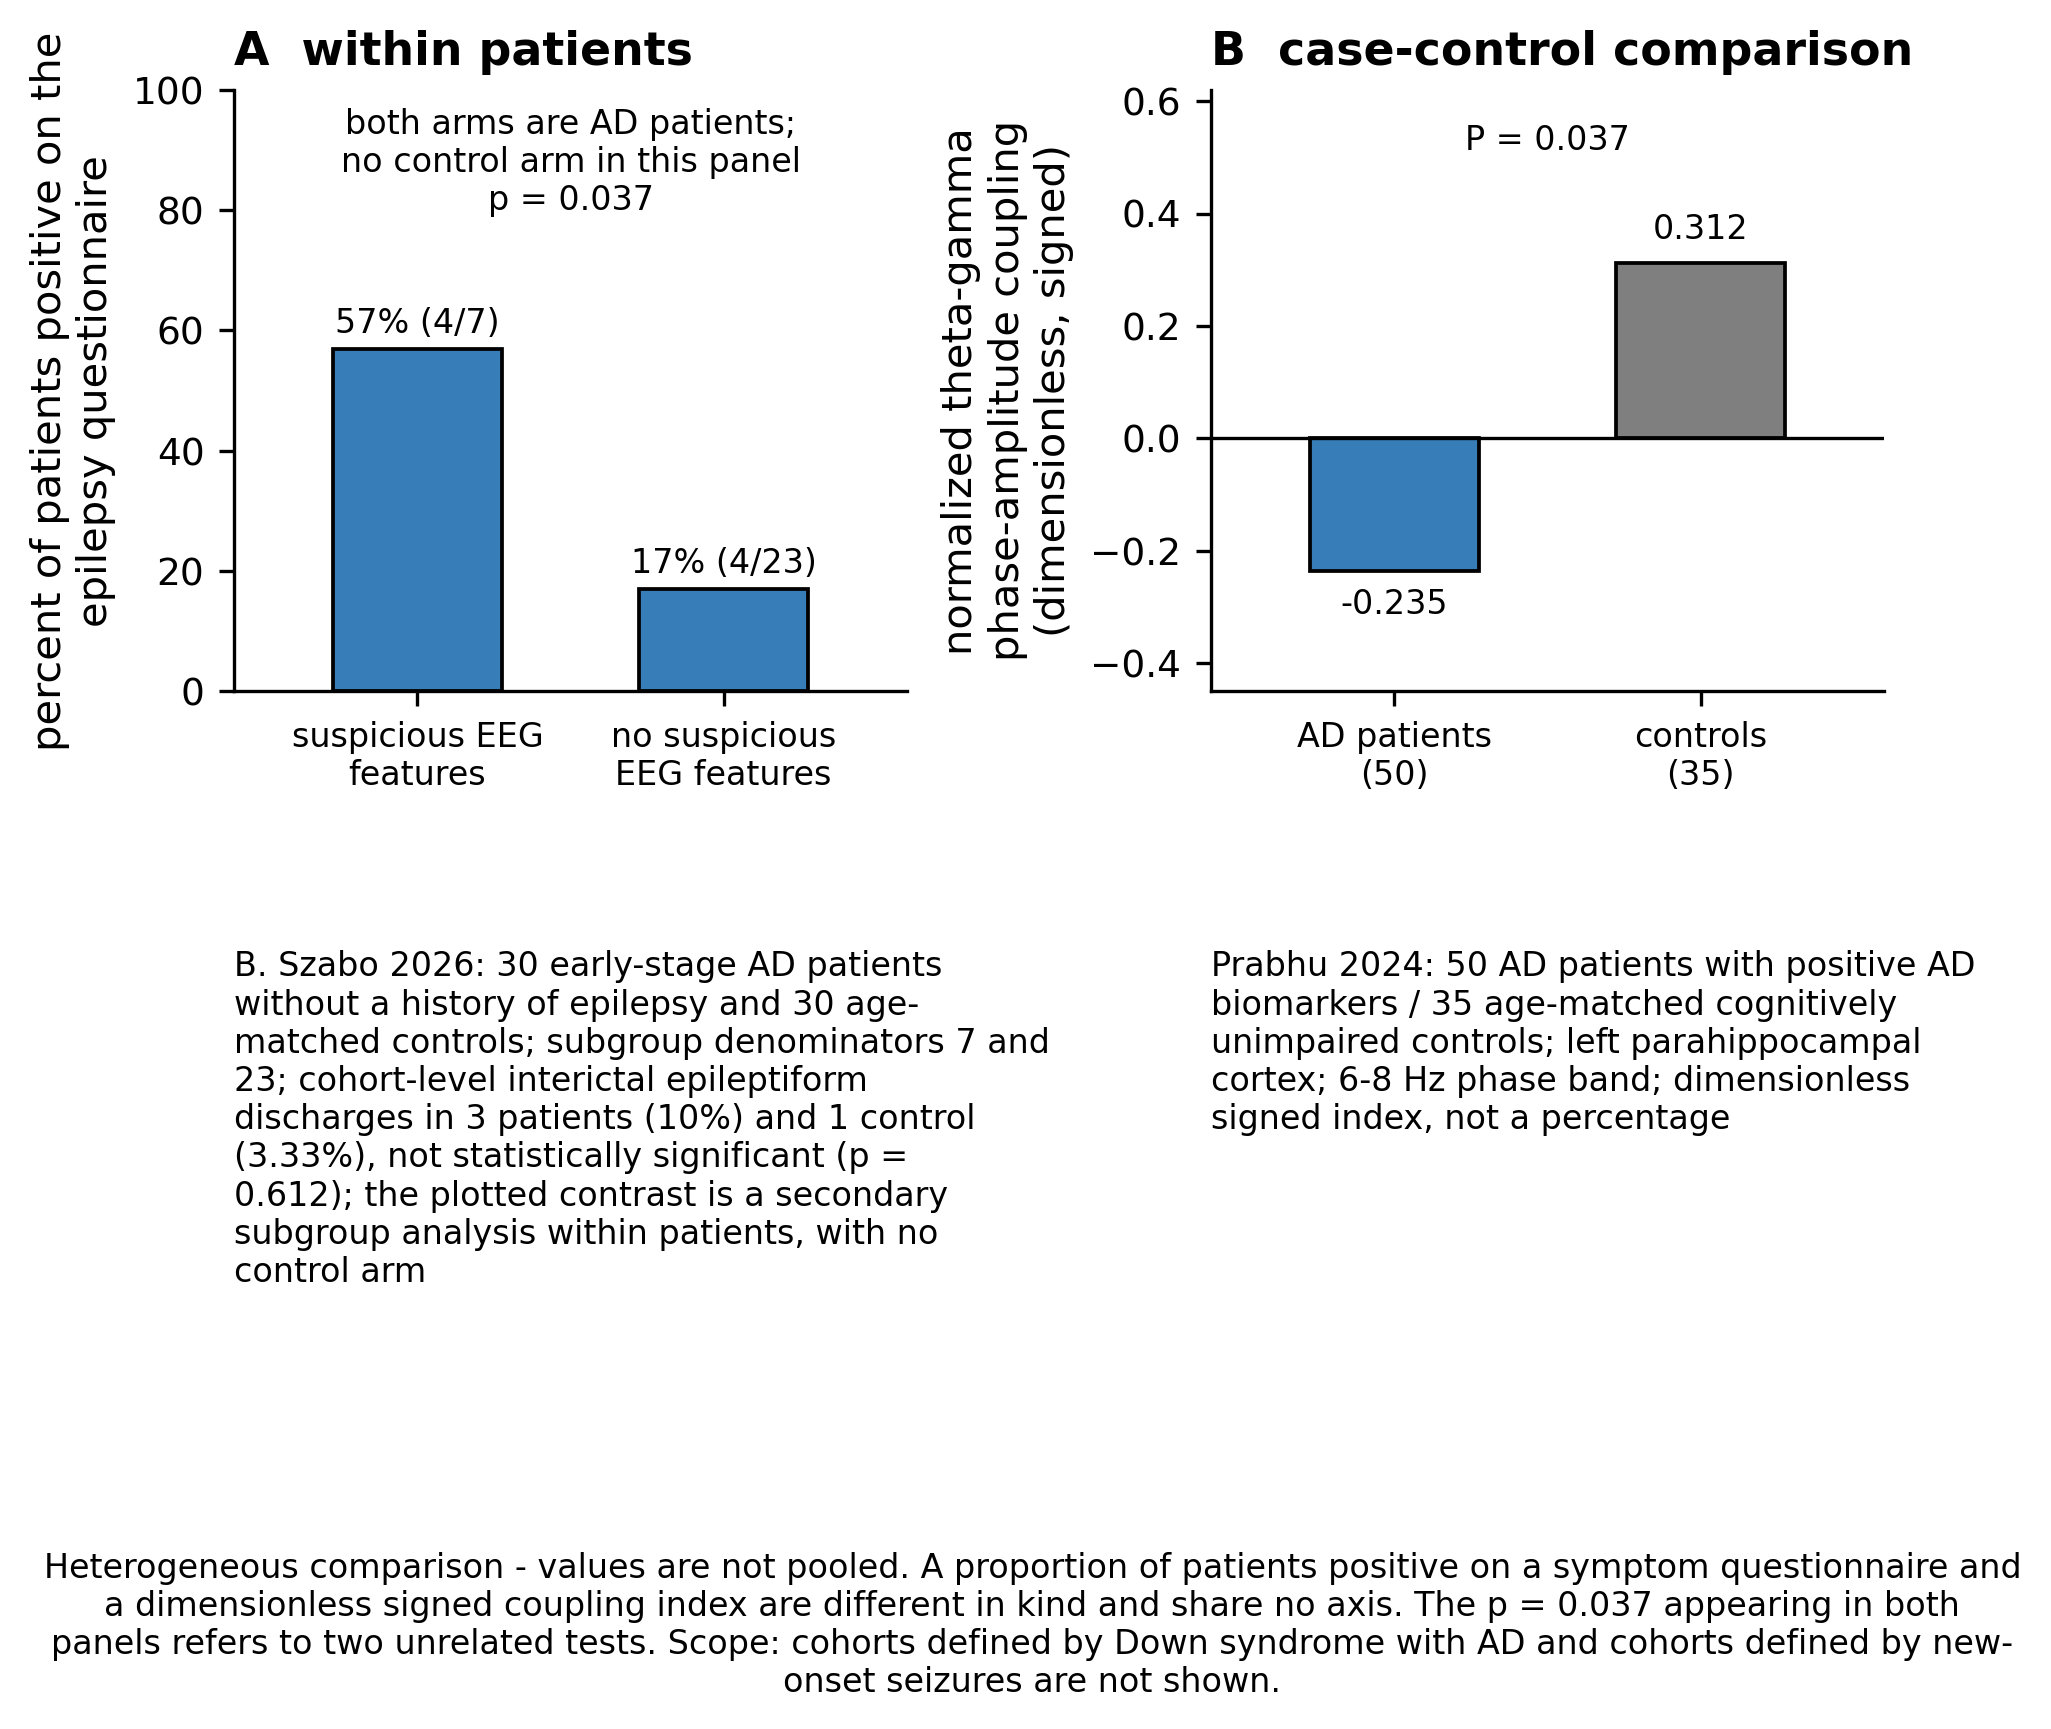
\includegraphics[width=\linewidth]{../figures/fig_sec4_human_hyperexcitability_markers.png}
\caption{\textbf{Two human readouts, two designs.} Human network-hyperexcitability measurements in AD on separate axes: the proportion of patients positive on an epilepsy symptom questionnaire, stratified by EEG suspicion status (A), and normalized theta--gamma phase-amplitude coupling in AD versus controls (B). Panel A is a within-patient stratification, not a case-control comparison: both arms are AD patients, split by the presence of suspicious EEG features (4 of 7 versus 4 of 23, of 30 patients studied), and the panel has no control arm. Panel B is a case-control comparison of 50 AD patients with 35 age-matched controls. \citet{BSzabo2026}'s plotted contrast is a secondary subgroup analysis; at cohort level interictal epileptiform discharges were detected in 3 patients (10\%) and 1 control (3.33\%), a difference that did not reach statistical significance (p = 0.612). The phase-amplitude coupling index is dimensionless and signed, computed for the left parahippocampal cortex in the 6--8 Hz phase band; it is not a percentage and shares no axis with panel A. The p = 0.037 appearing in both panels refers to two unrelated tests. Scope: cohorts defined by Down syndrome with AD and cohorts defined by new-onset seizures are not shown here. Heterogeneous comparison --- values are not pooled.}
\label{fig-sec4-human-hyperexcitability-markers}
\end{figure}

The mechanistic evidence that connects inhibition to this phenotype is almost entirely about parvalbumin cells. hAPP transgenic mice show spontaneous nonconvulsive seizure activity in cortical and hippocampal networks with GABAergic sprouting and enhanced synaptic inhibition in dentate gyrus \citep{Palop2007}, and restoring Nav1.1 in those mice increased gamma activity and reduced epileptiform discharges, with hAPPJ20/Nav1.1 mice showing fewer spikes than hAPPJ20 mice during low-intensity gamma activity \citep{Verret2012}. Levetiracetam suppressed the aberrant network activity and reversed hippocampal remodelling, synaptic and cognitive deficits in the same model family \citep{Sanchez2012}, interictal spikes in Tg2576 mice are state-dependent and cholinergically gated, with rates significantly higher in REM than wakefulness in n = 5 mice \citep{Scharfman2025}, and pharmacological disruption of the GSK3$\beta$/Nav1.6 complex dose-dependently suppressed epileptiform spiking during non-rapid-eye-movement (NREM) sleep, from 155.8 $\pm$ 11.79 spikes/h in vehicle to 90.46 $\pm$ 16.84 at 50 mg/kg (p = 0.0011) and 58.24 $\pm$ 11.16 at 75 mg/kg, with n = 3 animals per dose \citep{Baumgartner2025}. The structural substrate is also compartment-specific: A$\beta$ overexpression in aged animals was accompanied by a 58\% decrease in synapse density at CA1 basal dendrites relative to wild-type littermates \citep{Ray2024}, and laminar neural-mass modelling shows that progressively weakening fast-interneuron inhibition onto pyramidal cells reproduces the hallmark EEG slowing and hyperexcitability signatures of AD progression \citep{SanchezTodo2026}. How dendritic inhibition loss produces these oscillatory phenotypes is developed in \ref{sec-circuit-consequences}.

\begin{quote}
\noindent\textbf{Evidence Conflict}\par
\textbf{Is reduced Nav1.1 the mechanism of interneuron failure? (resolved by method, to the extent it is resolved).} \citet{Verret2012} attributes PV interneuron failure and network hypersynchrony in an amyloid model to reduced Nav1.1, and rescues discharges by restoring it. \citet{Kudo2023} finds fast-spiking interneurons selectively hypoactive in the rTg4510 tauopathy model, with excitatory neuron activity unchanged at 5--6 months, and states explicitly that the dysfunction cannot be explained by tau accumulation in interneurons or by altered Nav1.1 and Kv3.1b protein levels. The recorded axis is model construct and proteinopathy --- hAPPJ20 amyloid versus rTg4510 tau --- so the two results may both hold in their own systems; what they jointly exclude is a single channel-level account of inhibitory failure across proteinopathies. The rTg4510 exclusion of Nav1.1 and Kv3.1b has not been independently reproduced in the work retrieved by these searches.

\end{quote}

The step that this section cannot supply is the SST-specific one. No retrieved study tests whether restoring SST interneuron output alone normalises epileptiform activity, and the one available selective-loss manipulation argues against sufficiency: in otherwise healthy mice carrying no amyloid or tau pathology, conditional deletion of \emph{c-Maf} from cortical SST interneurons reduced their excitatory synaptic drive and density, yet \emph{Mafb} conditional knockouts with reduced SST interneuron density did not exhibit epileptiform activity \citep{Leroux2026}. The claim that SST interneuron loss causes network hypersynchrony in AD is therefore widely asserted but not demonstrated by the selective-loss model that exists, and the calcium-buffering route to tau-driven hyperexcitability --- calbindin-D28k downregulation in hippocampal excitatory neurons, with adeno-associated-virus (AAV)-mediated restoration reducing hyperexcitability and microgliosis \citep{Gao2026} --- locates the proximate defect outside the SST population altogether.

\subsection{Hyperactive or degenerating? SST interneuron state under amyloid}
\label{sec-04-hyperactive-or-degenerating}

Three readouts of the SST population under amyloid point in three directions, and the discrepancy is largely a matter of what was measured and under what exposure. In vivo two-photon calcium imaging of genetically labelled interneurons in APP/PS1 cortex found SOM interneuron event rates 2.7-fold higher than in wild-type, with SOM hyperactivity greatest near plaques, while PV interneurons in the same model showed a 1.8-fold decrease \citep{Algamal2022b,Algamal2022a}. Ultrastructural analysis of \emph{App} NL-F knock-in hippocampus found the opposite picture for the same class: 89\% of plaques (n = 45, 2 mice) carried SOM-positive dystrophic neurites and 93\% (n = 75, 2 mice) carried CB1R-positive dystrophic neurites, whereas only 4\% (n = 93, 2 mice) carried PV-positive ones \citep{Sos2020}. Acute exposure to soluble oligomers reverses the sign again: 250 nM soluble A$\beta$42 oligomers significantly reduced nicotine-induced activity in SST-positive interneurons (1.000 $\pm$ 0.391 to 0.600 $\pm$ 0.237 $\Delta$F/F$_{0}$, p = 0.0002) and in PV-positive interneurons (1.000 $\pm$ 0.772 to 0.448 $\pm$ 0.233 $\Delta$F/F$_{0}$, p = 0.0038), with co-activation of $\alpha$7 and $\alpha$4$\beta$2 nicotinic receptors reversing the deficit \citep{Lee2026}. Somatic calcium activity and axonal integrity are different quantities, and chronic fibrillar plaque exposure in awake cortex and acute soluble-oligomer application to hippocampal neurons are different exposures; reading these as a contradiction about "SST function in amyloid" collapses both distinctions, which is why \ref{fig-sec4-sst-activity-direction} separates the chronic and acute exposures. What is missing is the within-animal comparison --- spontaneous and cholinergically driven SST activity across the soluble-oligomer and plaque-bearing stages of the same model --- and no study pairing cell counts with physiological recording in the same animals or the same human tissue was retrieved by these searches, which is why structural-loss and activity studies are currently set against each other with no shared preparation.

\begin{quote}
\noindent\textbf{Evidence Conflict}\par
\textbf{Hyperactive, degenerating, or suppressed? (partially resolved for the first pair, open for the second).} \citet{Algamal2022a} reports a 2.7-fold increase in SOM interneuron calcium event rates in an APP model, while \citet{Sos2020} reports SOM-positive dystrophic neurites at 89\% of plaques with near-complete sparing of PV terminals --- functional hyperactivity against ultrastructural degeneration of the same population, reconcilable in principle because somatic calcium activity and terminal degeneration are different measurements. Separately, \citet{Algamal2022b}'s chronic plaque-bearing hyperactivity stands against \citet{Lee2026}'s suppression of nicotine-evoked activity in SST-positive interneurons after acute soluble oligomer exposure; the recorded axis is model construct and species transfer, and the therapeutic polarity --- silence SST cells or boost them --- cannot be settled from the present evidence. \citet{Algamal2022a} and \citet{Algamal2022b} are the journal and preprint reports of one imaging study, so the same result stands on both sides of this layout.

\end{quote}

\begin{figure}[H]
\centering
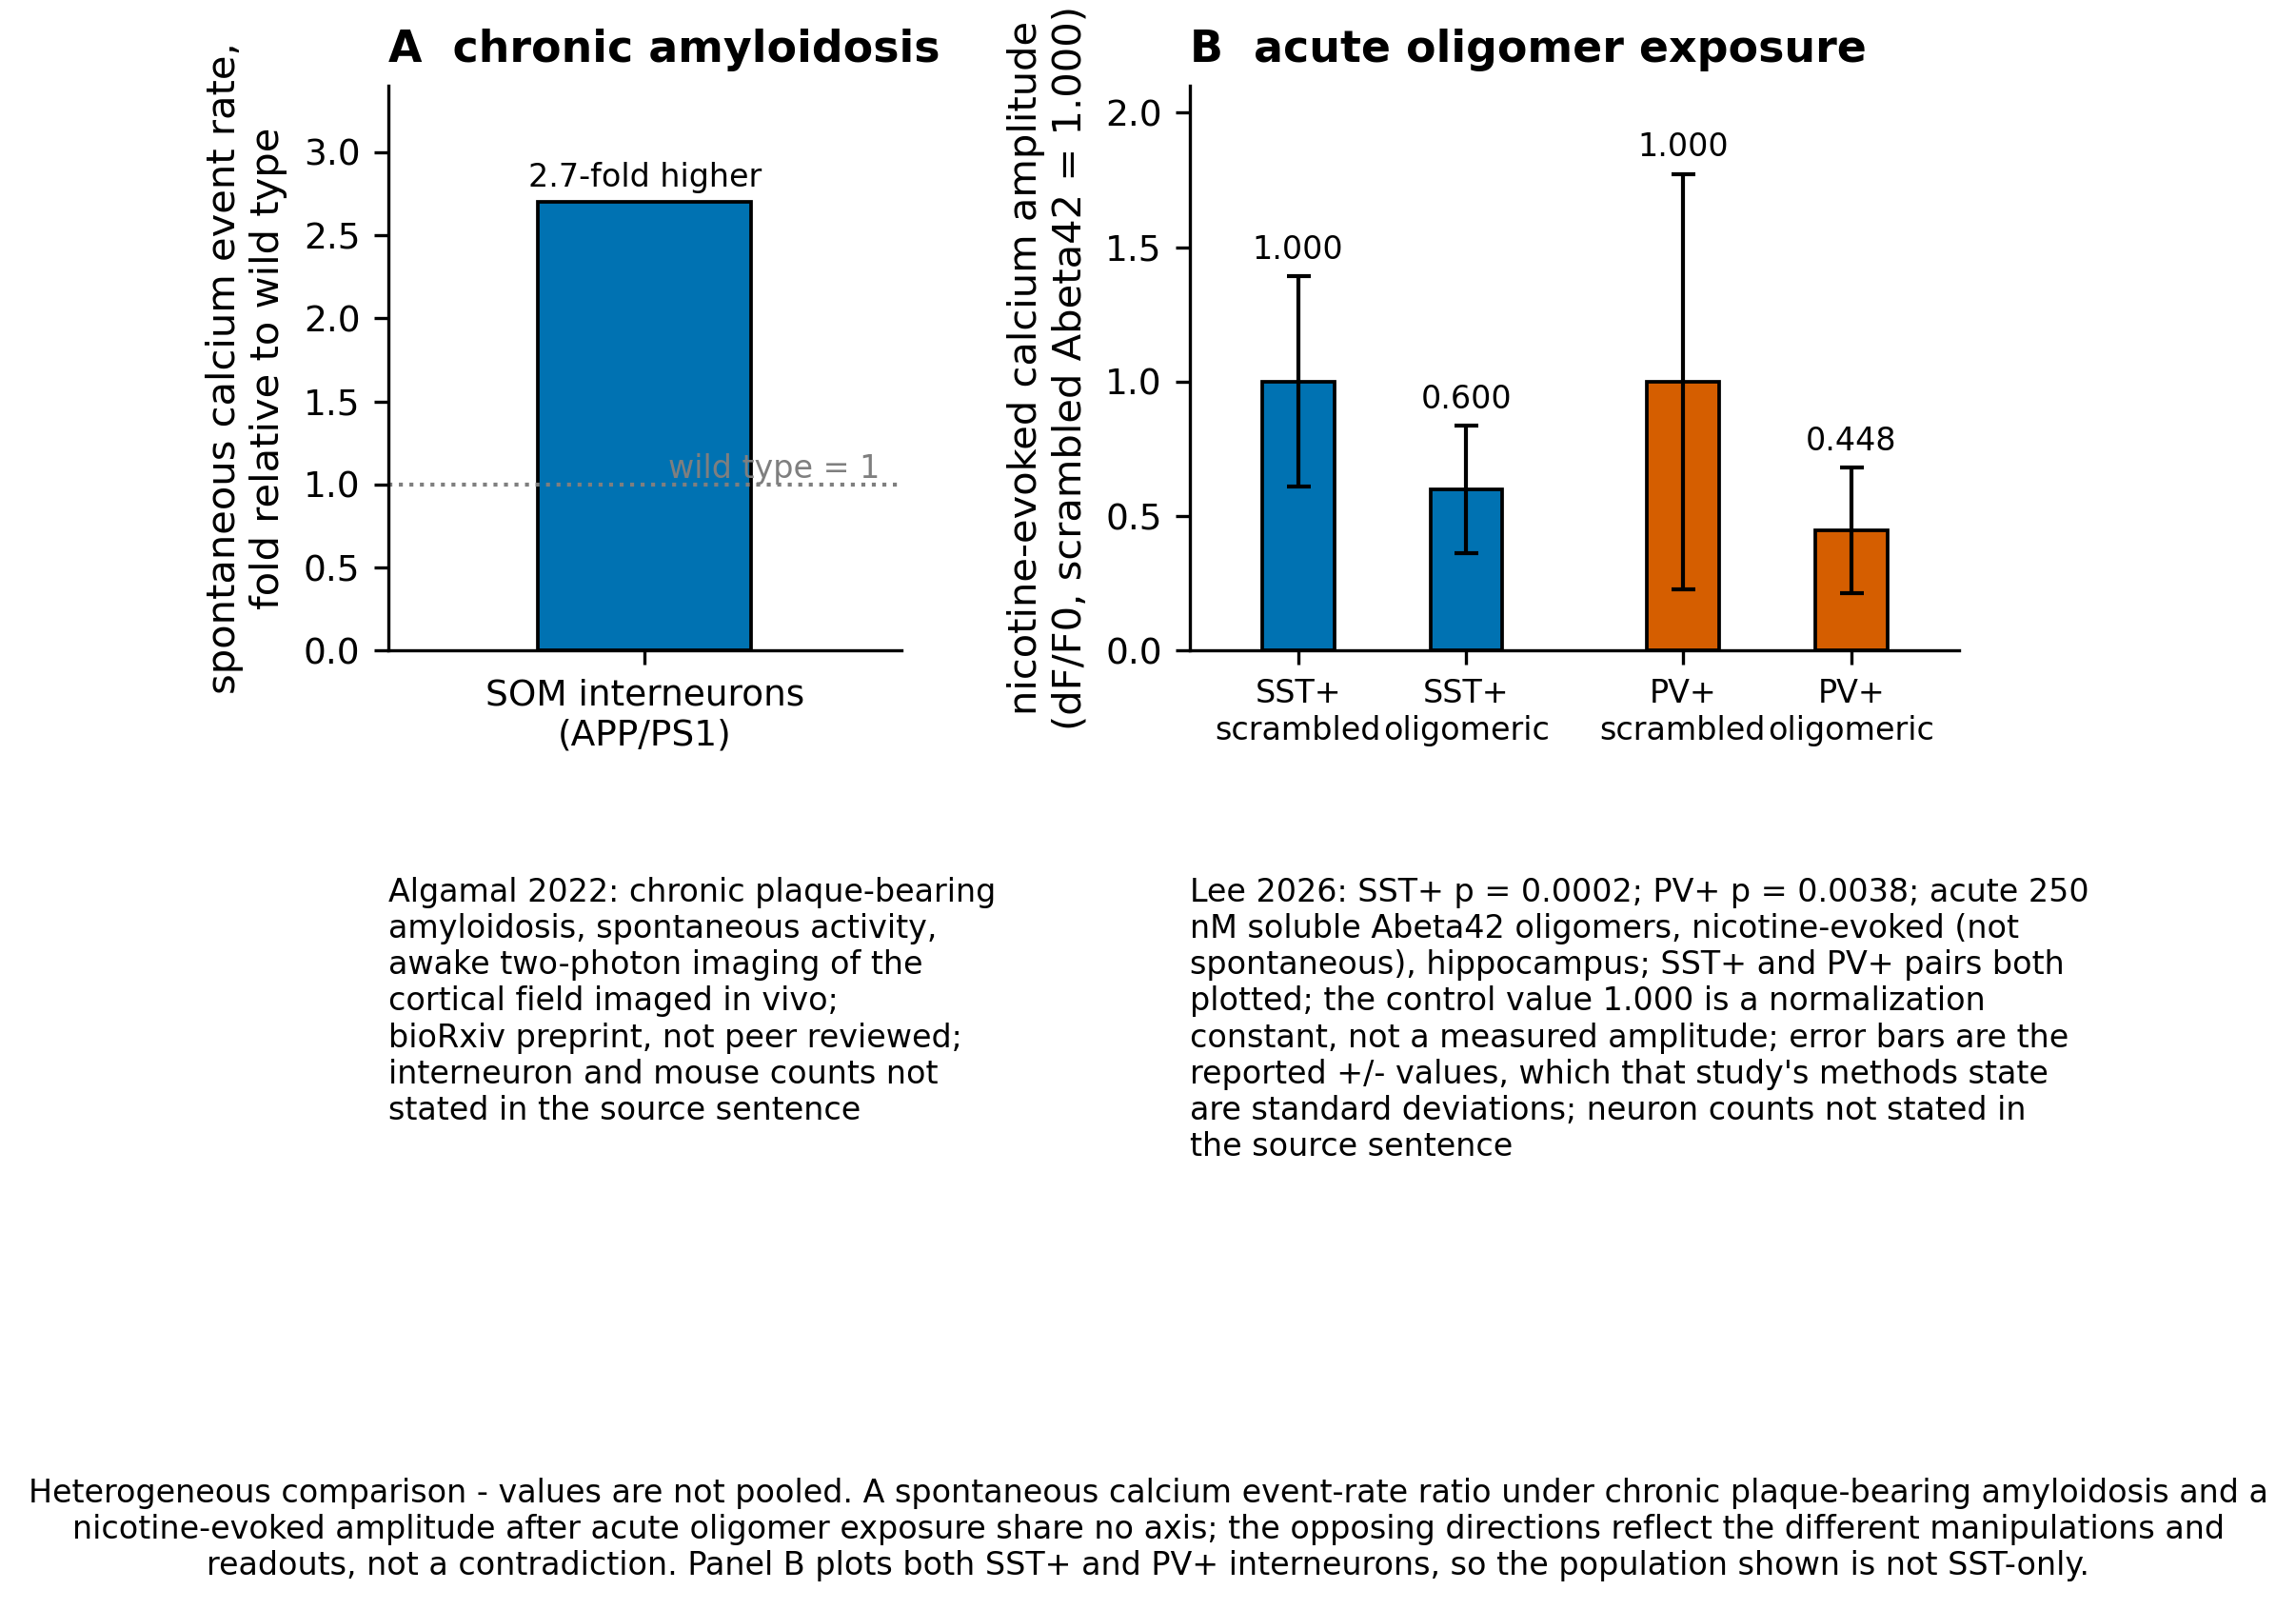
\includegraphics[width=\linewidth]{../figures/fig_sec4_sst_activity_direction.png}
\caption{\textbf{Direction depends on the exposure.} SST interneuron physiology under amyloid, with chronic and acute exposures on separate axes: spontaneous calcium event rate as a fold ratio to wild type in chronic plaque-bearing amyloidosis (A), and nicotine-evoked calcium amplitude after acute oligomer exposure, normalized to the scrambled-A$\beta$42 control (B). The two panels are not commensurate --- a spontaneous calcium event-rate ratio recorded in the cortical field imaged in vivo under chronic plaque-bearing amyloidosis, and a nicotine-evoked amplitude after acute 250 nM oligomer exposure in hippocampus --- and the opposing directions reflect the different manipulations and readouts, not a contradiction. Panel B plots both SST-positive and PV-positive interneurons, so the population shown in this figure is not SST-only. \citet{Lee2026}'s control value of 1.000 $\Delta$F/F$_{0}$ is a normalization constant, not a measured amplitude; no percentage reduction is reported in the source and none is drawn. The dispersion values reported by \citet{Lee2026} ($\pm$ 0.391 and $\pm$ 0.237) are standard deviations, which that study's methods state, and the error bars are labelled accordingly. \citet{Algamal2022b} is a bioRxiv preprint and has not been peer reviewed, and the units of analysis of the two entries differ (interneurons imaged versus neurons imaged). Heterogeneous comparison --- values are not pooled.}
\label{fig-sec4-sst-activity-direction}
\end{figure}

Functional manipulations give the SST population a specific and partly separable role in the oscillatory phenotype. Optogenetic activation of SST-positive but not PV-positive interneurons fully restored the peak power of theta oscillations and resynchronized theta spike phases in amyloid-oligomer-injected hippocampus, with PV activation restoring gamma power instead and the two deficits traced to dissociable presynaptic mechanisms --- reported in the preprint and published versions of the same experiments \citep{Chung2018,Chung2020}. The synaptic locus is not the SST cell's own input or output: oligomers had no effect on pyramidal-to-SST or SST-to-pyramidal synapses but specifically disrupted SST interneuron-mediated disinhibition, impairing theta-nested gamma oscillation-induced spike-timing-dependent potentiation \citep{Park2020}. Supplying new inhibitory cells rather than modulating the surviving ones also restores function --- transplanting human iPSC-derived medial-ganglionic-eminence inhibitory neurons into 5xFAD hippocampus raised the novel-object discrimination index from 0.36 to 0.62 (p = 0.0017) against a wild-type value of 0.55, with novel-arm entries increased by 24.4\% (p = 0.0198), at three months post-transplant and with no significant improvement at two months \citep{Zhang2026a} --- although that graft is a mixed GABAergic population with a behavioural endpoint, so the benefit cannot be attributed to SST cells. The gamma-entrainment programme occupies the same circuit space from the PV side: driving fast-spiking PV interneurons at 40 Hz, and non-invasive 40 Hz flicker, reduced A$\beta$1--40 and A$\beta$1--42 and mitigated plaque load \citep{Iaccarino2016}, auditory and audiovisual stimulation extended the effect to hippocampus and to phosphorylated tau in a P301S model \citep{Martorell2019}, and clearance-side and coordination-side mechanisms have since been added, with multisensory 40 Hz stimulation increasing cortical CSF tracer influx and meningeal lymphatic vessel diameter \citep{Murdock2024} and 40 Hz flicker raising CA3--CA1 slow-gamma phase coordination by 184\% for pyramidal cells and 130\% for interneurons during virtual navigation \citep{Paulson2025}.

\begin{quote}
\noindent\textbf{Evidence Conflict}\par
\textbf{Why does 40 Hz stimulation help? (unresolved; carried forward).} \citet{Iaccarino2016} attributes the benefit to frequency-specific entrainment that lowers A$\beta$ levels and plaque load. \citet{Aguilera2025} reports that two weeks of 40 Hz visual stimulation in 4-month-old \emph{App}/\emph{MAPT} double knock-in mice --- an age at which the same study confirms no significant plaque deposition --- restores impaired global EEG network dynamics to wild-type-comparable levels and rescues object-in-place memory, and proposes a non-amyloid mechanism that is not necessarily 40 Hz-specific. The disagreement is about mechanism rather than about whether the intervention works, and is taken up with the rest of the stimulation literature in \ref{sec-therapeutics}.

\end{quote}

\subsection{What the AD evidence can and cannot support}
\label{sec-04-what-the-evidence-supports}

The audited position is narrower than the literature's summary of itself. A reduction in the somatostatin signal in AD cortex is established in direction across the retrieved record, reproduced by independent groups across four decades in tissue radioimmunoassay \citep{Davies1981,Rossor1980,Arai1984,Mazurek1991}, cerebrospinal fluid assay \citep{Soininen1984,Atack1988,Urakami1989}, cortical and hippocampal cell counting \citep{Gaspar1989,GonzalezRodriguez2021}, and transcriptomic deconvolution and single-nucleus sequencing \citep{Consens2022a,Consens2022b,Castanho2025b}. Nothing beyond direction survives the same scrutiny. The magnitudes are measured on non-interconvertible scales, the regional panels behind the early cohorts differ from near-global to focal, and the two single-nucleus and deconvolution cohorts frame the cells differently rather than oppositely: \citet{Consens2022b} reports the SST-annotated inhibitory population proportionally depleted in AD, while \citet{Castanho2025b} describes SST interneurons as a vulnerable population that is maintained in cognitively resilient individuals --- a difference of cohort framing, not of direction. The causal mechanism most often attached to the deficit is credible, has a receptor-level and a downstream-effector arm \citep{Nilsson2020,Nilsson2025,Watamura2021,Watamura2020}, and has a direct in vivo refutation on the record from the one amyloid knock-in cross that tested it \citep{Williams2023,Williams2022}. No human study that manipulates or longitudinally tracks SST interneuron number alongside amyloid load was retrieved by these searches, so the causal direction rests entirely on rodent \emph{Sst} knockout and agonist work --- which matters because the therapeutic rationale for SST-receptor agonists assumes that the rodent ordering transfers to humans.

Several claims in this section carry a replication status that their circulation does not reflect, and they are flagged here rather than smoothed. The original result that somatostatin regulates brain A$\beta$42 by upregulating neprilysin activity \citep{Saito2005} has not been independently reproduced in a knock-in amyloid model in the work retrieved here, and the single in vivo test on that background is negative on the enzyme \citep{Williams2023}. The mixed somatostatin--A$\beta$ oligomeric assembly with a residue-specific effect on fibrillization kinetics \citep{Solarski2018}, the brain-penetrant somatostatin fusion protein that raises hippocampal neprilysin and lowers A$\beta$42 \citep{Rofo2021}, the endoplasmic-reticulum-stress origin of SST neuron vulnerability \citep{Tomoda2022}, the exclusion of Nav1.1 and Kv3.1b as the cause of fast-spiking interneuron hypoactivity in rTg4510 \citep{Kudo2023}, and the superior protection of octreotide and lanreotide over native somatostatin against A$\beta$42 toxicity \citep{Pham2025} are each single, uncorroborated observations in the material assembled here. Three further limits are structural rather than evidential. Retrieval was dominated by one bibliographic source with no citation chasing, so every absence stated in this section is an absence in what these searches returned rather than in the literature. Full text was available for 61 of 112 papers in the Alzheimer's disease literature surveyed here, the shortfall falling on exactly the pre-2000 closed-access postmortem and cerebrospinal fluid series that carries the foundational claim, so the regional and methodological detail behind those cohorts is read at abstract level. The searches for disconfirming results were capped, so the disagreements presented here are a top-relevance sample rather than a census. And eleven of the works cited in this section carry preprint or preprint-server identifiers rather than journal ones, several of them load-bearing: both parties to the receptor-arm neprilysin disagreement \citep{Nilsson2020,Williams2022}, the only SST-specific oscillatory rescue \citep{Chung2018}, the soluble-versus-insoluble A$\beta$ assignment \citep{Sasaguri2021}, the $\alpha$-endosulfine regulator \citep{Watamura2020}, the $\alpha$5-GABA-A result \citep{Dharavath2024}, the peptidomic resilience result \citep{Morgan2024b}, the microRNA route to neprilysin \citep{Wang2026}, the SOM hyperactivity imaging \citep{Algamal2022b}, and the preprint halves of the two human transcriptomic cohorts \citep{Consens2022a,Castanho2025a}.

AD therefore supplies the template that the rest of this review tests: a reproducible peptide deficit, a contested cellular interpretation, and a mechanistic chain whose therapeutic consequences are being drawn before its central step has been replicated. \ref{sec-parkinsons-lewy-body} asks whether the same pattern appears in a different proteinopathy, and finds that the cortical deficit reported there may be imported from Alzheimer co-pathology rather than generated by $\alpha$-synuclein.

\section{Parkinson's Disease and Lewy Body Dementias}
\label{sec-parkinsons-lewy-body}

The cortical somatostatin deficit established in \ref{sec-alzheimers} has a contested cellular interpretation, and Lewy body disease provides the natural test of whether that deficit is specific to Alzheimer-type pathology.

\subsection{Cortical somatostatin is conditional on Alzheimer-type co-pathology}
\label{sec-05-cortical-copathology}

The post-mortem record answers that the deficit tracks dementia; whether it additionally requires Alzheimer-type pathology cannot be settled from these series, because the two that report reductions selected cases carrying that pathology \citep{Beal1986d,FlintBeal1988} and the Lewy-body-type dementia series do not report co-pathology status \citep{Whitford1988,Leake1991}; the occipital series is the exception, staining for $\alpha$-synuclein, A$\beta$ and hyperphosphorylated tau and excluding cases with high coexisting Alzheimer pathology \citep{Khundakar2016}. \citet{Beal1986d} measured somatostatin-like immunoreactivity (SLI) by radioimmunoassay in post-mortem tissue from 15 control patients, 7 non-demented parkinsonian patients and 7 demented parkinsonian patients who had Alzheimer-type cortical pathology: the non-demented cases had normal SLI concentrations in cerebral cortex, hippocampus, amygdala, putamen, caudate or globus pallidus, while the demented cases with Alzheimer-type pathology showed reductions of approximately 40\% in frontal (Brodmann area 6) and temporal (Brodmann area 21) cortex. \citet{FlintBeal1988}, sampling 12 control patients and 13 demented parkinsonian patients with Alzheimer-type cortical pathology across twenty-two cortical regions, found significant SLI reductions in 17 regions, typically 50-60\%, against neuropeptide Y (NPY) reductions of 20-30\% in nine regions --- a dissociation between two peptides that are co-expressed in the same cortical interneuron class, as set out in \ref{sec-sst-identity}. The 1988 series shares its first author, and one further author, with the 1986 one and extends it to a larger region set, so the two are best read as a within-group replication rather than as two independent confirmations; whether they draw on shared case material is not stated in the retrieved text. \citet{Leake1991} separated the syndromes directly, reporting that somatostatin was reduced only in temporal cortex in senile dementia of the Lewy body type and in senile dementia of the Alzheimer type, and unaltered in Parkinson's disease (PD) without dementia. The pattern is therefore indexed by dementia and co-pathology, not by a parkinsonian diagnosis, and this is the reading that \citet{Leake1993} and \citet{Beal1990} draw from the same literature, with the caveat that both are secondary accounts rather than new measurements. An older series reported decreased cortical SLI in all six cases of pathologically confirmed diffuse Lewy body disease alongside profound neocortical choline acetyltransferase loss \citep{Dickson1987}; whether those cases also carried Alzheimer-type cortical pathology is the variable that determines how much weight the result can bear.

Two observations constrain the generality of the deficit. The modern dementia with Lewy bodies (DLB) series of \citet{Khundakar2016} measured somatostatin by ELISA in primary visual cortex and found it unchanged in DLB (p = 0.40, uncorrected) and in AD (p = 0.09, uncorrected), while neuropeptide Y was increased by approximately 20\% in AD only (p = 0.027, uncorrected); \citet{Leake1991} reports reduction only in temporal cortex, which implies but does not state an occipital null. Region, not diagnosis, separates these nulls from the temporal and frontal reductions; \ref{fig-sec5-cortical-somatostatin-conditional-on-copathology} arranges every series along the cognitive and neuropathological axis and keeps the magnitude and direction-only entries on separate panels. The second constraint is the absence of cell counts: every primary series above measures bulk peptide, the only morphological statement in this record being the qualitative one relayed by \citet{Beal1990}, that somatostatin neurons in both illnesses are markedly dystrophic and may be reduced in number; and no study quantifying somatostatin-immunoreactive neuron numbers stereologically in DLB or Parkinson's disease dementia (PDD) neocortex was retrieved by these searches, nor any series of pure Lewy body disease in which Alzheimer-type pathology was excluded or covaried. Reduced peptide and reduced cell number are therefore not separable here, which is the central interpretive ambiguity of the cortical literature and the reason this section speaks of reduced somatostatin-like immunoreactivity rather than of interneuron loss.

\begin{quote}
\noindent\textbf{Evidence Conflict}\par
\citet{FlintBeal1988} report SLI reductions of typically 50-60\% across 17 of twenty-two cortical regions in demented parkinsonian patients, whereas \citet{Whitford1988} measured both SLI and high-affinity [3H]somatostatin binding sites in frontal (Brodmann area 9) and temporal (Brodmann area 21) cortex in presenile and senile Alzheimer's disease and in mentally normal and cognitively impaired cases of Parkinson's disease, and found no significant changes between any of the disease groups --- and the authors suggest that somatostatinergic involvement is not a consistent or primary neurochemical feature of these diseases. The disagreement is not one of assay: both are radioimmunoassay series of the same era. It turns on whether the sampled cases carried concomitant Alzheimer-type cortical pathology and on which regions were taken. Because the Whitford cohort includes cognitively impaired parkinsonian cases, its null bears directly on the Beal result rather than describing a different population. Resolution status: partially resolved --- the co-pathology explanation is consistent with both datasets, but no cohort stratified on Alzheimer-type pathology was retrieved by these searches.

\end{quote}

\begin{figure}[H]
\centering
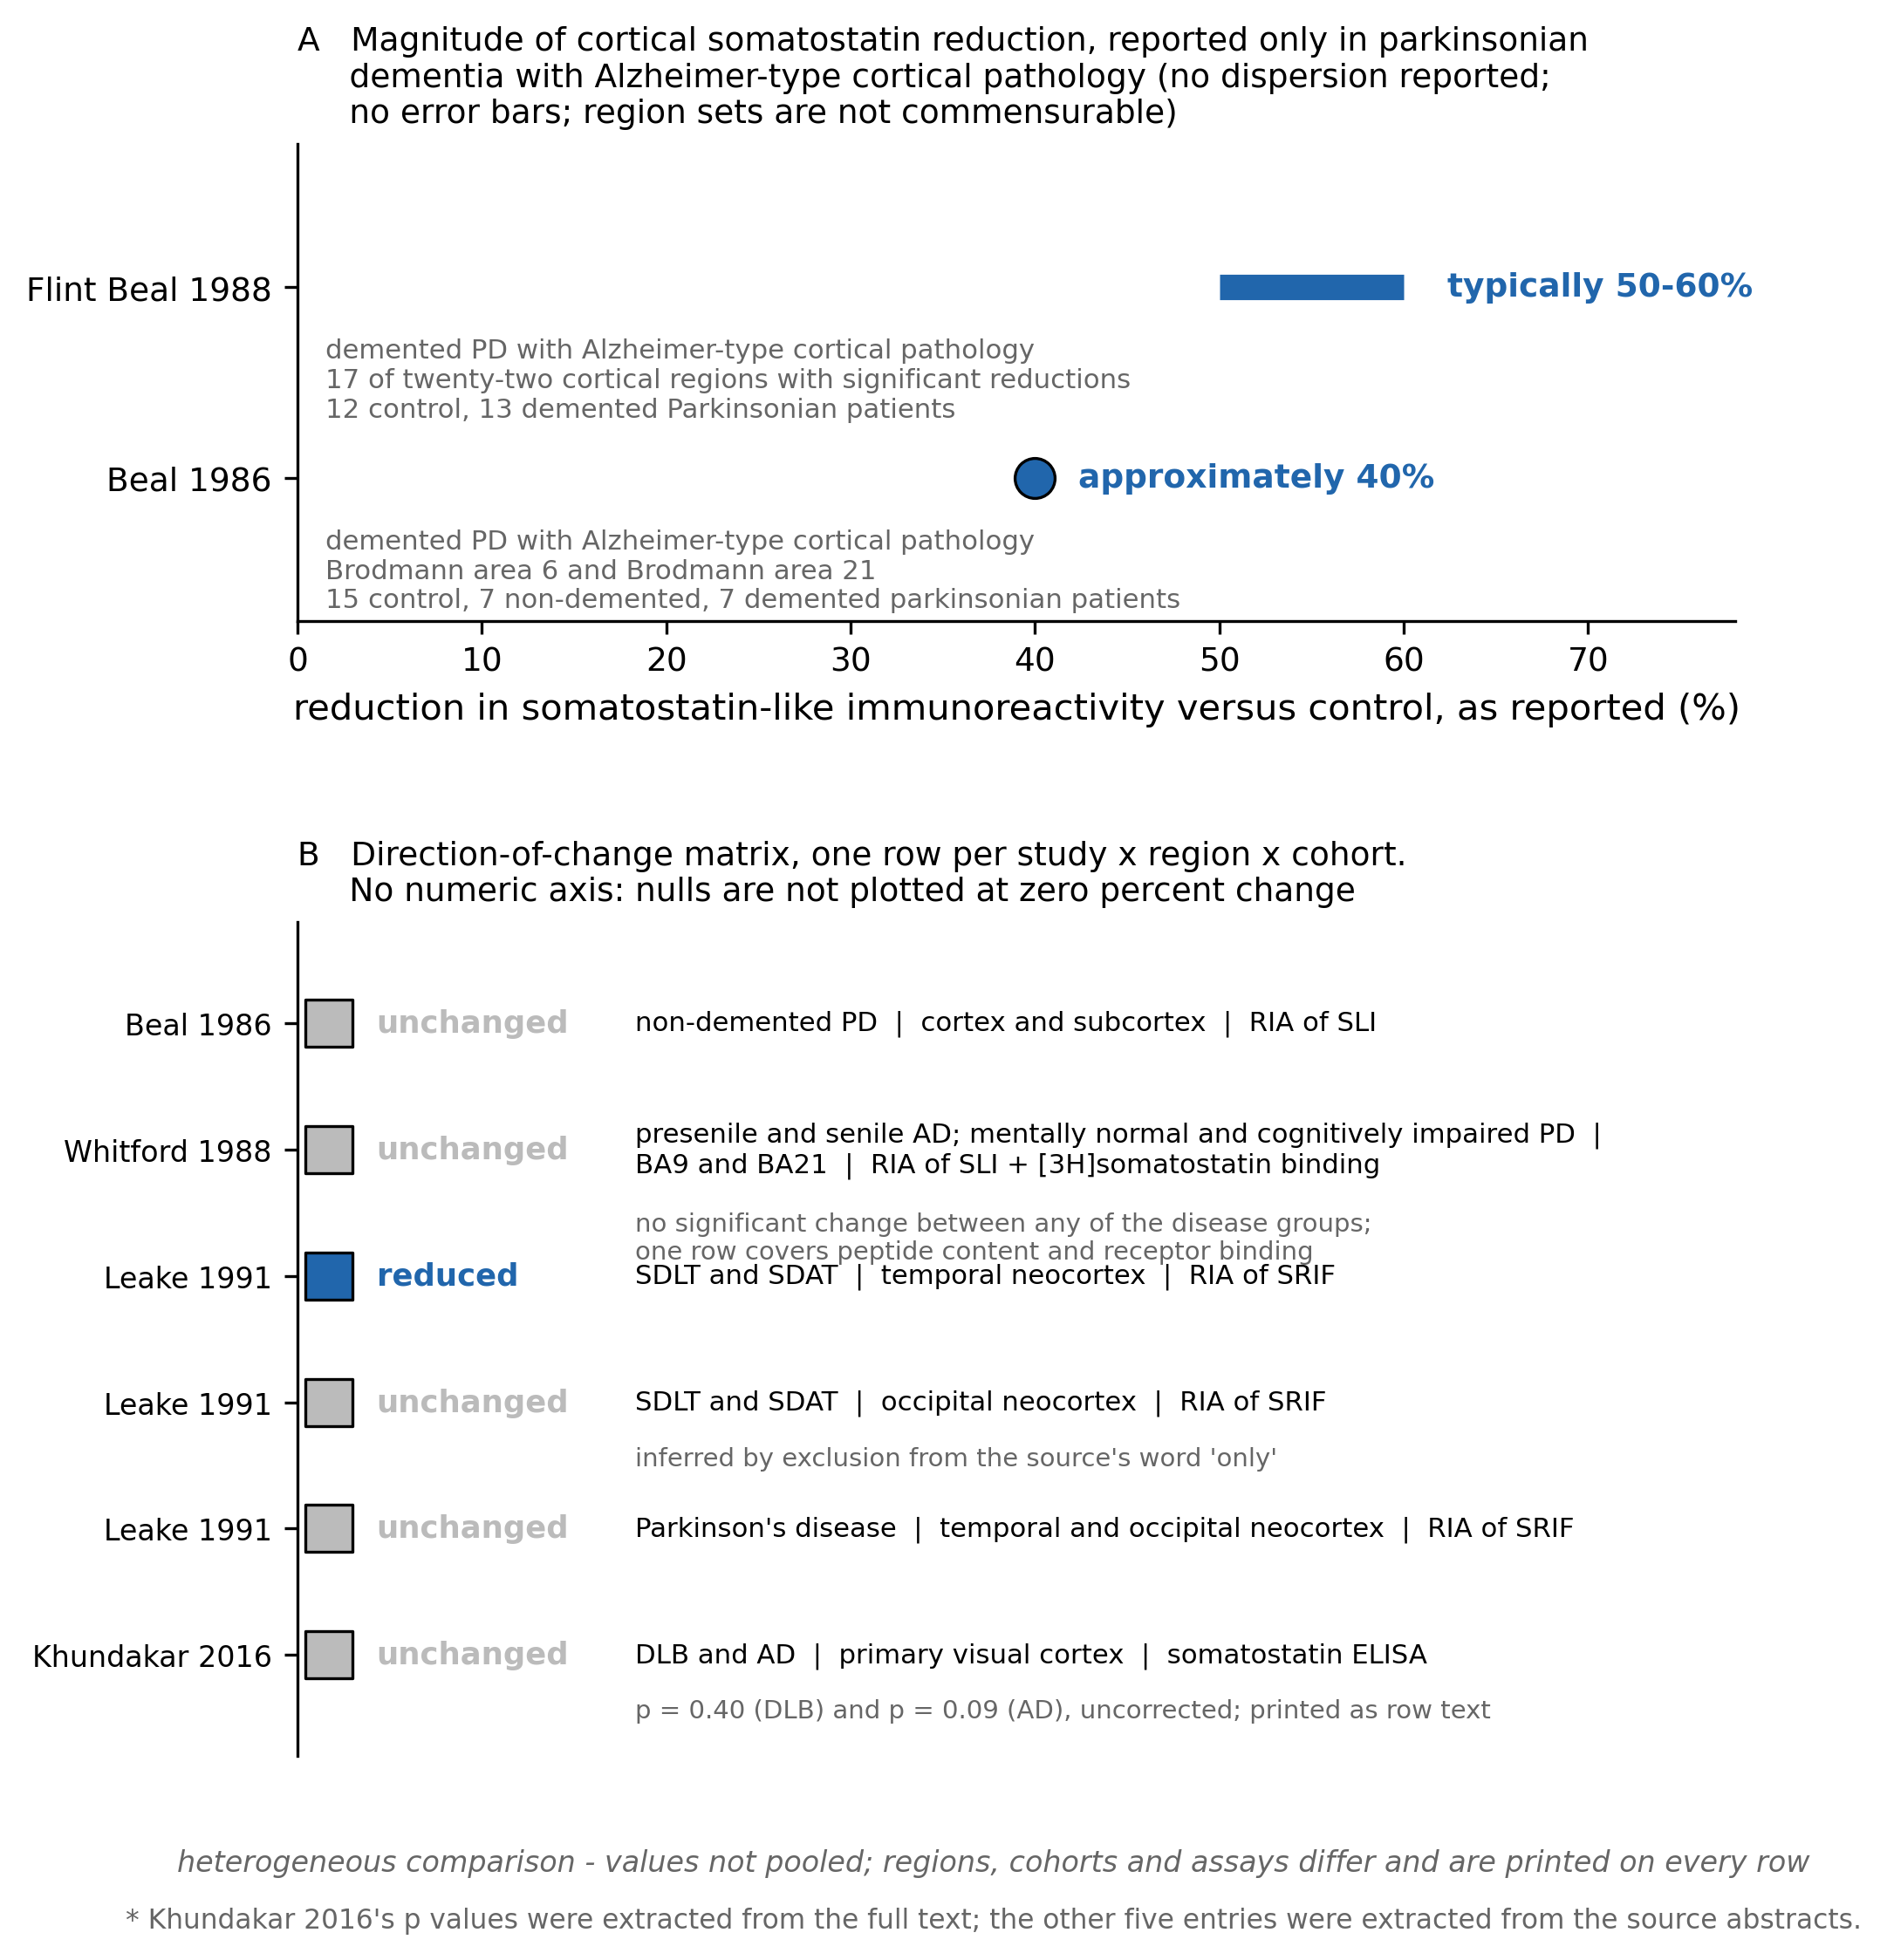
\includegraphics[width=\linewidth]{../figures/fig_sec5_cortical_somatostatin_conditional_on_copathology.png}
\caption{\textbf{Cortical somatostatin in Lewy body disease, by cognitive and neuropathological status.} Panel A shows the two series that report a magnitude; panel B resolves every series into one row per study, region and cohort and reports direction only. Panel A caveats: Flint Beal 1988's 50-60\% is the typical magnitude among the 17 of twenty-two cortical regions with significant reductions, not a mean over all regions examined, while Beal 1986's approximately 40\% is for Brodmann area 6 and Brodmann area 21 only; both bars come from cases with concomitant Alzheimer-type cortical pathology, and the same studies report normal cortical somatostatin in non-demented Parkinson's disease, shown in panel B; group sizes are given as reported per group (12 control and 13 demented Parkinsonian patients; 15 control, 7 non-demented and 7 demented parkinsonian patients), neither value carries an error term, and no test of the difference between the two studies exists; the 1988 series extends the 1986 one to a larger region set under the same first author, so the two are better read as a within-group replication than as two independent confirmations; whether they share case material is not stated in the retrieved text, and the two study labels are two renderings of the same first author's name. Panel B caveats: the cortical reductions in panel A are reported only in demented parkinsonian cases with concomitant Alzheimer-type cortical pathology; Whitford 1988 examined presenile and senile Alzheimer's disease together with mentally normal and cognitively impaired cases of Parkinson's disease and found no significant change in somatostatin-like immunoreactivity or [3H]somatostatin binding, so because its cohort includes cognitively impaired Parkinson's disease cases its null bears directly on, and partly conflicts with, the reductions in panel A; Whitford 1988's quoted finding is an absence of significant change between any of the disease groups, which the source reports after comparison with an age- and post-mortem-delay-matched normal group, and one row carries both peptide content and receptor binding under a single reported outcome; the Leake 1991 occipital row is inferred from the source's word "only" ("SRIF was reduced only in temporal cortex"), not from an explicit occipital statement, and is marked as inferred; regions are not matched across studies, and primary visual cortex is reported unchanged in Khundakar 2016 while the occipital null in Leake 1991 is inferred from its word "only" rather than stated, so region is printed on every row; Whitford 1988 and Leake 1991 contribute a direction only, not a magnitude, and are shown categorically and not as zero percent change; assays differ, with radioimmunoassay of somatostatin-like immunoreactivity in the four older series versus somatostatin ELISA in Khundakar 2016, whose p values are uncorrected, printed as row text and derived from full text, while Whitford 1988 additionally reports [3H]somatostatin binding; among the panel B rows, group sizes are reported in the source only for Beal 1986 and are not printed in that panel, whereas panel A prints the per-group counts of both of its entries; they are unreported in the retrieved abstracts for Whitford 1988 and Leake 1991 and are not stated in the text retrieved for Khundakar 2016, so absence of a detected change is not evidence of absence of change. Sources: \citep{Beal1986d,FlintBeal1988,Whitford1988,Leake1991,Khundakar2016}.}
\label{fig-sec5-cortical-somatostatin-conditional-on-copathology}
\end{figure}

\subsection{Cerebrospinal fluid somatostatin: a direction that will not stabilise}
\label{sec-05-csf-direction}

The fluid literature does not converge, and the way it fails to converge is informative. Three cohorts report reduced somatostatin-like immunoreactivity in parkinsonian patients --- lumbar cerebrospinal fluid at 19.8 +/- 9.0 fmol/ml against 32.5 +/- 12.0 fmol/ml in senile controls \citep{Cramer2008}, CSF at 21.4 +/- 8.1 fmol ml-1 in 38 aged parkinsonian patients against 29.5 +/- 9.4 fmol ml-1 in senile controls \citep{Strittmatter1992}, and lateral ventricular fluid at 42.9 +/- 2.9 fmol/ml against 65.3 +/- 9.7 fmol/ml in benign essential tremor patients \citep{Cramer1985a} --- and a fourth reports cerebroventricular SLI significantly lower in Parkinson's disease than in neurological controls with chronic stable multiple sclerosis or temporal lobe epilepsy \citep{Jost1990}. Against these, \citet{Espino1995} measured CSF-SLI in twenty-three untreated patients with parkinsonian syndrome at diagnosis, 15 of them with idiopathic Parkinson's disease, and found it significantly \emph{higher} than in 26 subjects without neurological symptoms (107.9 +/- 9.8 pg/ml versus 73.5 +/- 8.4 pg/ml). That elevation remains unreplicated three decades after publication and is the single result that prevents the fluid literature from being read as a monotonic decline. Laying the cohorts side by side in \ref{fig-sec5-csf-somatostatin-parkinson-cohorts} shows that the direction of change co-varies with fluid compartment, disease stage, comparator group and assay units rather than with a consistent biomarker signal; because units differ and somatostatin-like immunoreactivity is a mixed peptide pool, only within-study contrasts are interpretable, and no conversion between the fmol/ml and pg/ml cohorts is defensible.

\begin{quote}
\noindent\textbf{Evidence Conflict}\par
Two disagreements sit inside this literature. First, \citet{Jolkkonen1986} found CSF SLI lower than controls in 36 patients with early Parkinson's disease and 19 controls (p < 0.01), with the lowest values in demented parkinsonian patients, while \citet{Volicer1986} found SLI similar in parkinsonian patients and controls. Both are contemporaneous radioimmunoassay series, so assay modality is held constant and the residual explanations are cohort cognitive status and disease stage; status: open. Second, \citet{Espino1995} report elevation in untreated early parkinsonian syndrome while \citet{Masson1990}, studying 35 aged patients (mean 79.5 y) against 11 controls (mean 82.3 y), report SLI lower than controls (P < .02) and \emph{lowest in the untreated group}. Disease duration, control-group composition and the reported unit all differ, so assay calibration cannot be excluded; status: unresolved. A third, softer tension --- CSF somatostatin rising early while cortical tissue somatostatin falls late \citep{Kasprzak2026,Beal1990} --- may not be a contradiction at all if fluid peptide reflects release from degenerating tissue rather than tissue stores, but no longitudinal within-subject CSF series spanning untreated parkinsonism to dementia was retrieved by these searches, so the two cross-sectional patterns cannot be reconciled from the available record.

\end{quote}

One widely repeated claim deserves explicit correction. CSF somatostatin is often described as a marker of cognitive decline in Parkinson's disease, yet the cohorts that tested the association directly do not support it: \citet{Strittmatter1992} found SLI correlated with motor disease progression and \emph{not} with dementia scores, in explicit contrast to Alzheimer-type dementia, and \citet{Masson1990} found only non-significant trends toward lower values with greater motor severity and lower Mini-Mental State scores. \citet{Jolkkonen1986} reported the lowest values in demented patients, but as a subgroup observation within a cross-sectional design. No study linking baseline CSF somatostatin to incident PDD was retrieved, and \citet{Thakur2025} identify somatostatin as among the least investigated neuropeptide biomarker candidates for the diagnosis of Parkinson's disease generally, without addressing Parkinson's disease dementia. The biomarker argument is taken up in \ref{sec-human-evidence}; here the point is that a frequently asserted association rests on data that, where tested, point the other way.

\begin{figure}[H]
\centering
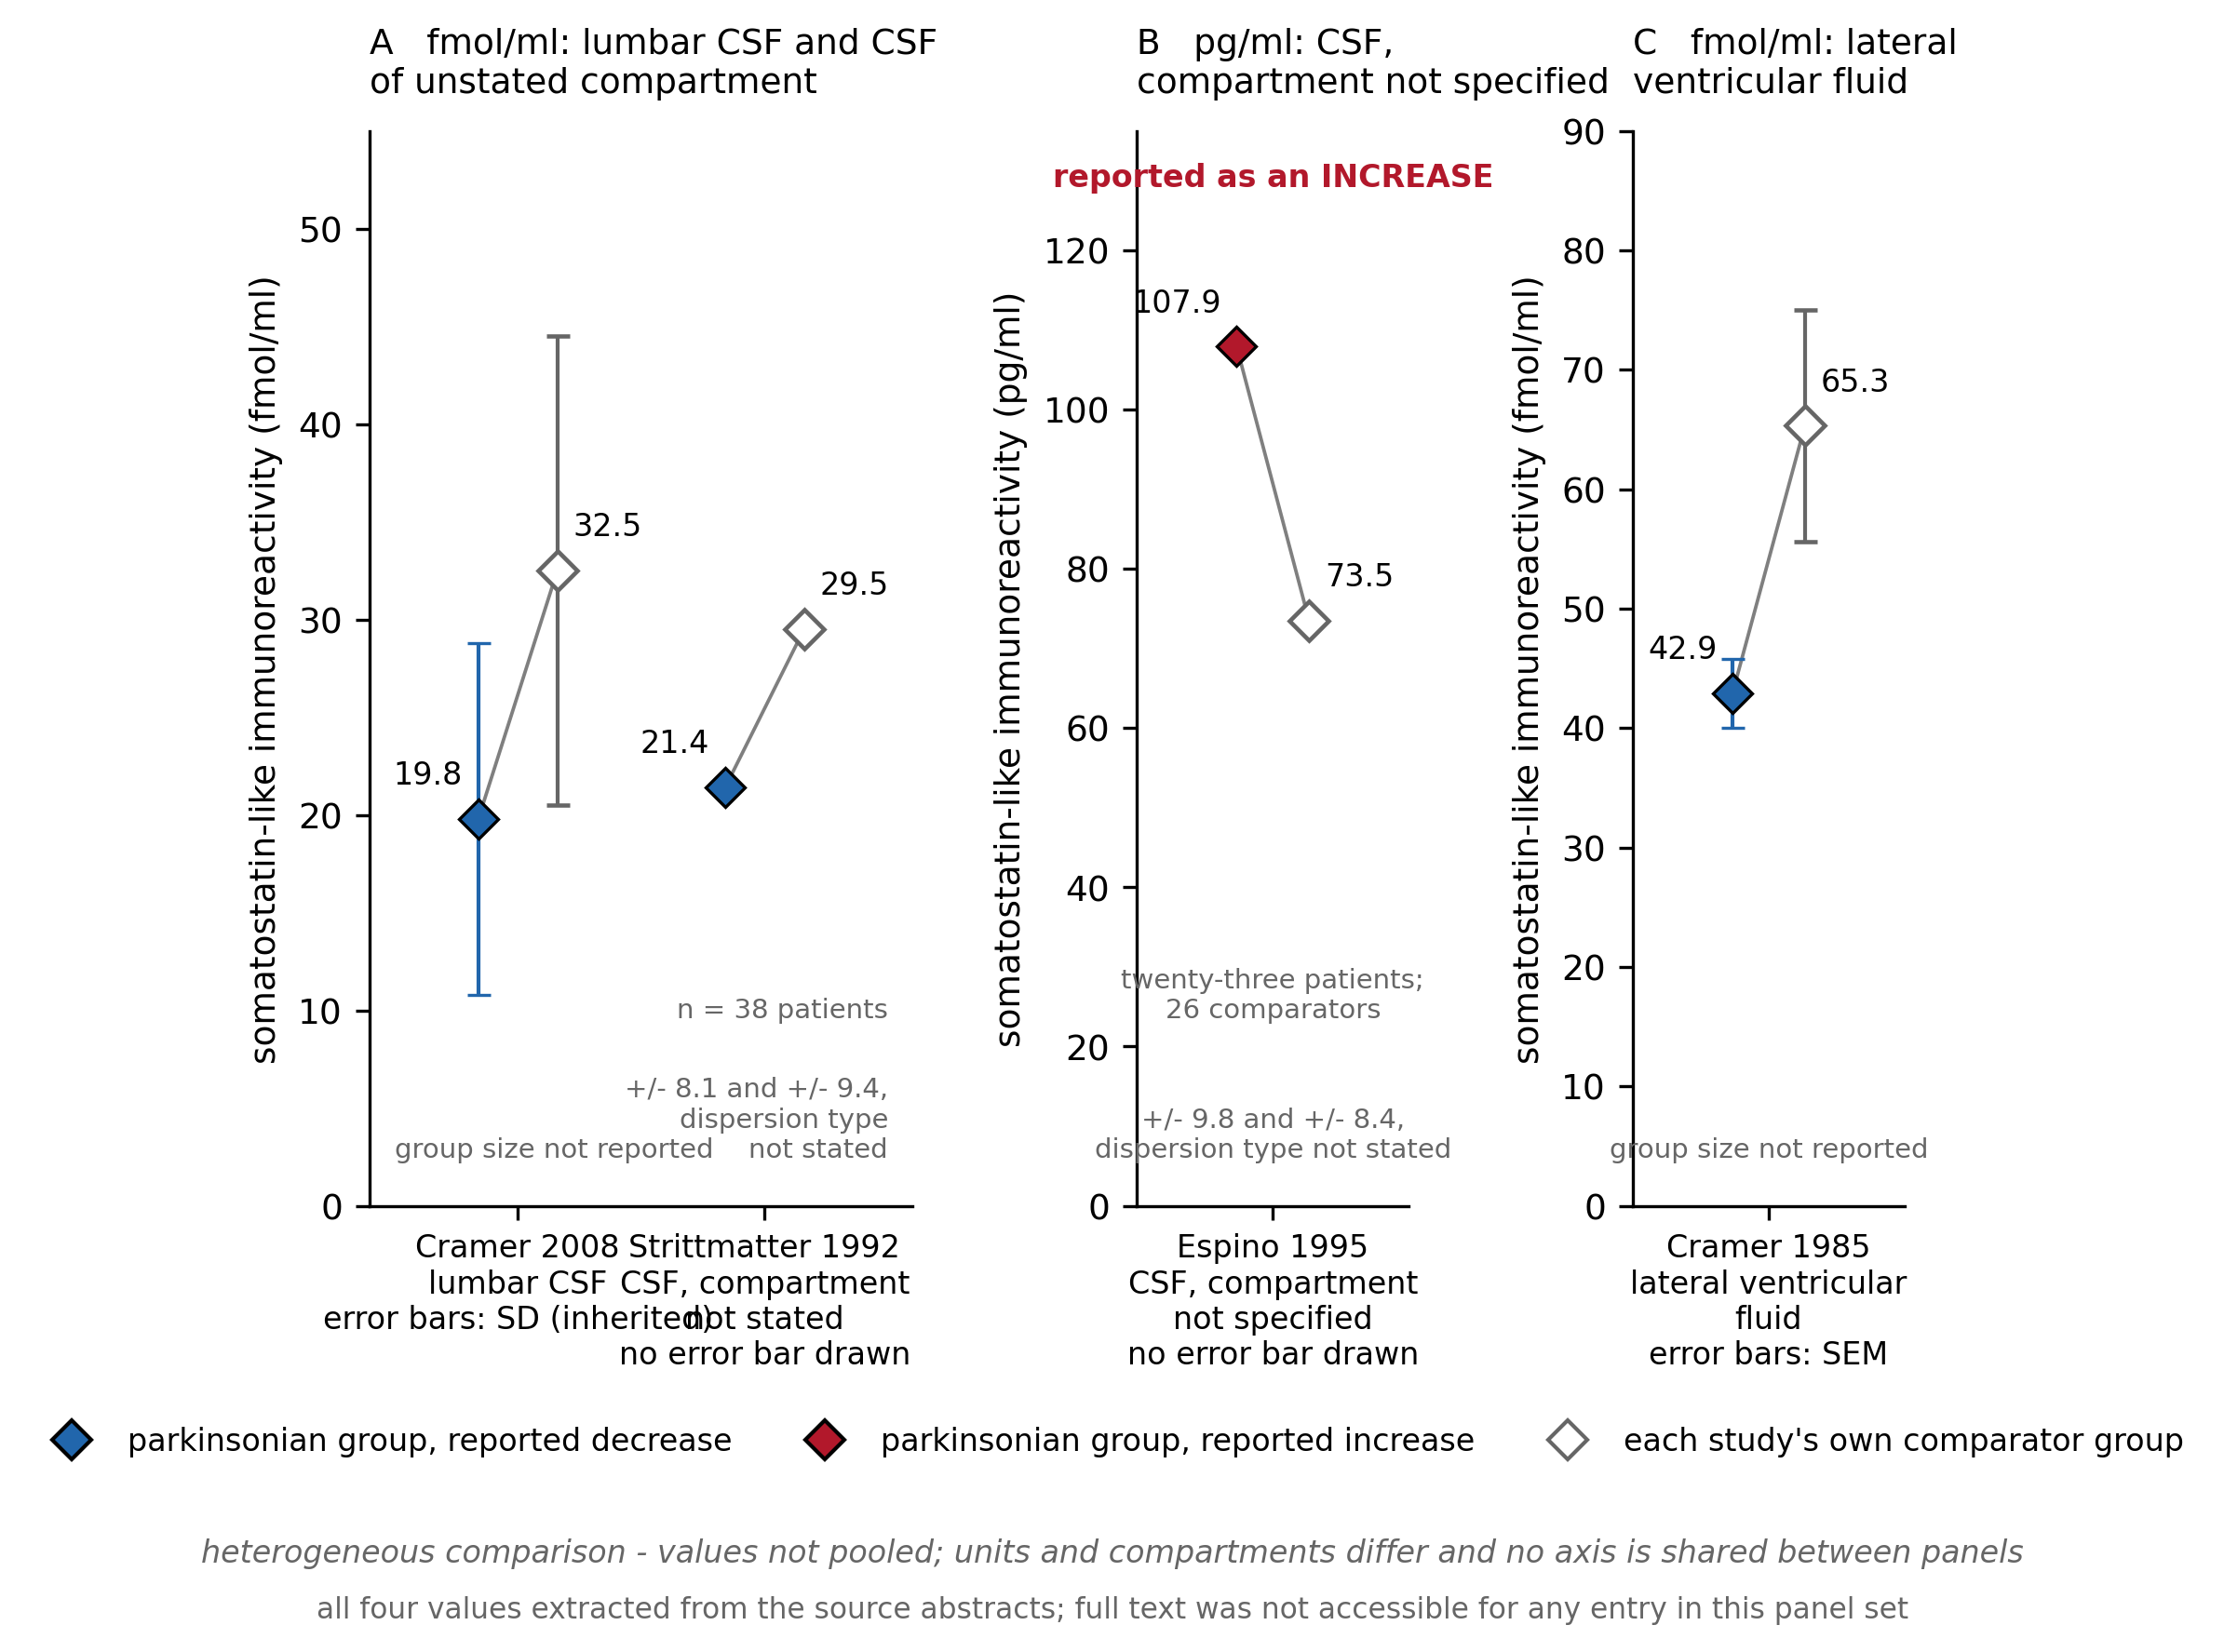
\includegraphics[width=\linewidth]{../figures/fig_sec5_csf_somatostatin_parkinson_cohorts.png}
\caption{\textbf{Fluid somatostatin in parkinsonian cohorts, shown by compartment and unit.} Patient and comparator means are plotted as reported, each panel with its own unit and axis. Values are somatostatin-like immunoreactivity measured by radioimmunoassay in different fluid compartments; lumbar and ventricular concentrations are not interchangeable and are shown in separate panels with separate axes. Panel A pairs a study that states its compartment with one that does not: Cramer 2008 reports lumbar spinal fluid, while Strittmatter 1992's source reports only "cerebrospinal fluid (CSF)" and never names the compartment. Espino 1995 reports an increase, not a decrease, in untreated de novo parkinsonian syndrome and is reported in pg/ml; it occupies its own panel and must not be read as part of a monotonic decline. Comparator groups differ: senile control patients (Cramer 2008; Strittmatter 1992), benign essential tremor patients (Cramer 1985), and 26 subjects without neurological symptoms (Espino 1995). Error bars are drawn only where the source names the dispersion type: SEM for Cramer 1985, and SD for Cramer 2008 with the caveat that the "(SD)" is stated in that sentence for the substance-P value and inherited by the somatostatin values; Strittmatter 1992 and Espino 1995 name no dispersion type, so their +/- terms are printed as text and no error bar is drawn, and group sizes are not reported for Cramer 2008 and Cramer 1985. The Espino 1995 mean is the whole twenty-three-patient mixed parkinsonian-syndrome mean, of whom 15 had idiopathic Parkinson's disease and 8 had other forms of parkinsonism; the source states the dementia exclusion only for the idiopathic subgroup. Sources: \citep{Cramer2008,Strittmatter1992,Espino1995,Cramer1985a}.}
\label{fig-sec5-csf-somatostatin-parkinson-cohorts}
\end{figure}

\subsection{The striatal somatostatin/NPY/NOS system under dopamine depletion}
\label{sec-05-striatal-system}

In the striatum the question changes from how much peptide remains to what the cells are doing, and the answer separates structural from functional claims. The reported effect of dopaminergic denervation on striatal somatostatin is null in both series retrieved here, neither of which states a group size, so the nulls cannot be separated from low statistical power: \citet{Salin1990} found the number and topographical distribution of somatostatin-immunoreactive perikarya unaltered by unilateral 6-hydroxydopamine (6-OHDA) lesion or by alpha-methylparatyrosine-induced depletion, with no change in striatal somatostatin concentration by radioimmunoassay, and \citet{FlintBeal1983} found no effect of nigral 6-hydroxydopamine or ibotenic acid lesions or pallidal hemisection on striatal SLI while intrastriatal kainic acid depleted it by 60\% ipsilaterally and 25\% contralaterally --- locating about half of striatal SLI to intrinsic neurons. What does move the peptide is pharmacology and intrinsic damage rather than denervation, as \ref{fig-sec5-striatal-somatostatin-by-manipulation-class} sets out. In 6-OHDA-lesioned rats, \citet{Engber1992} showed that prolonged dopamine-receptor stimulation drives striatal somatostatin in both directions depending on receptor subtype and dosing regimen: intermittent D1 agonist SKF 38393 reduced somatostatin by 61\% against lesioned vehicle-treated controls, continuous D2 agonist quinpirole raised it by 43\%, intermittent quinpirole lowered it by 35\%, and continuous SKF 38393 did not alter it. Neuropeptide Y, the co-expressed marker of the same interneuron class, behaves as a more reactive readout, rising after 6-OHDA \citep{Lei2016,Maeda1993} and after MPTP \citep{Obuchowicz2003}, while \citet{Nitsch1993} found NPY-immunoreactive striatal neuron counts falling contralateral to a nigrostriatal lesion, in a manner dependent on the state of the striato-nigro-thalamic loop rather than on denervation alone.

The human striatal data run the other way from the rodent nulls and are thinner than their frequent citation suggests. \citet{Eve1997} reported a selective increase in somatostatin mRNA in the parkinsonian basal ganglia, and \citet{Cannizzaro2003} found more NPY mRNA-expressing cells with higher per-cell signal in PD striatum; \citet{Chesselet2007}, by contrast, summarises the rodent literature as showing striatal somatostatin mRNA decreasing after dopaminergic lesions and increasing after cortical ischaemic lesions, a direction conflict that remains contested. \citet{Kasprzak2026} relays a large reduction in striatal pre-prosomatostatin messenger RNA in aged rats, but the primary study is not identified in the retrieved text and the observation is one of ageing rather than parkinsonism. The only quantitative human counts come from two small series that disagree, and modern unbiased stereology of SST-, NPY- and nitric-oxide-synthase-expressing striatal interneurons in human Parkinson's disease using cell-type-specific markers rather than NADPH-diaphorase histochemistry was not retrieved by these searches. Every mechanistic model that assumes these interneurons survive and change function therefore rests, on the human side, on two contradictory five-case series.

\begin{quote}
\noindent\textbf{Evidence Conflict}\par
\citet{Bockelmann1994} quantified NADPH-diaphorase histochemistry in post-mortem putamen and reported control 1,120 +/- 69 per mm2 (n = 5) versus PD 575 +/- 164mm2 (n = 5) --- a claim of roughly halved density that has not been replicated in the thirty-two years since publication. \citet{Mufson1994} reported that striatal NADPH-diaphorase-containing neurons are spared in Parkinson's and Alzheimer's disease, with shrunken or bulbous somata and foreshortened dendrites but a significant cell-area reduction only in Alzheimer putamen. Both use the same histochemistry on small post-mortem series, so marker choice does not explain the difference; what differs is the counting denominator --- a ratio of stained neurons to total cells versus absolute counts --- and case selection. The source wording of the first study is itself internally inconsistent, describing a ratio while printing per-mm2 units, and that discrepancy is reproduced rather than repaired in \ref{fig-sec5-striatal-sst-system-under-dopamine-loss}. Resolution status: unresolved. A second disagreement is about direction: rodent striatal peptide content is unchanged after denervation \citep{Salin1990} while human basal ganglia show a selective increase in somatostatin transcript \citep{Eve1997}. Species, modality (peptide content versus mRNA) and chronicity all differ; status: unresolved.

\end{quote}

Function, by contrast, is reported to change sharply, on the evidence of one laboratory. \citet{LopezHuerta2012} recorded antidromically evoked inhibitory postsynaptic currents between spiny projection neurons in rat neostriatal slices and found that exogenous somatostatin presynaptically reduced these currents by \textasciitilde{}34\% in all control synapses tested; after dopamine deprivation, presynaptic inhibition grew to a 57\% reduction in \textasciitilde{}53\% of evoked currents recorded from direct-pathway neurons, while somatostatin produced an 82\% enhancement in \textasciitilde{}43\% of currents recorded from indirect-pathway neurons. A peptide that uniformly dampens feedback inhibition in the intact striatum thus acquires opposite signs on the two output pathways after denervation --- a single-laboratory result, unreplicated in fourteen years, whose implications for the direct/indirect imbalance are large enough that replication matters. Converging evidence that somatostatinergic signalling gains influence after denervation comes from microdialysis, where somatostatin-evoked striatal acetylcholine release is roughly twice as effective after 6-OHDA lesion \citep{Rakovska2003}. Behaviourally, intrastriatal somatostatin dose-dependently inhibits apomorphine-induced rotation in lesioned rats and the effect is blocked by cyclo-somatostatin \citep{Lu2002}, though that study tested lesioned animals only and so does not itself compare the intact and denervated striatum. Blockade of brain somatostatin signalling produces catalepsy in aged but not young rats, reversed by octreotide \citep{Ionov2012}. Around this peptidergic change the wider interneuron network is also reorganised: GABAergic drive onto NPY-expressing interneurons increases with giant and bursting spontaneous currents after dopamine depletion in a result reported by one laboratory \citep{Rubi2020}; perisomatic parvalbumin connectivity onto projection neurons is differentially remodelled \citep{Gomez2019}; interneuron-to-projection-neuron connectivity switches, including cholinergic innervation of striatopallidal neurons \citep{Salin2009}; cortical input and GABAergic interneurons imbalance projection-neuron discharge independently of dopamine \citep{Mallet2006}; medium calretinin interneuron density falls from 370 +/- 41 to 158 +/- 15 neurons/mm3 while small calretinin cells are unchanged \citep{Petryszyn2021}; tyrosine hydroxylase interneurons shift their firing profile \citep{Unal2013}; parvalbumin expression intensity falls rapidly during the second week after lesion \citep{He2024}; and striatal acetylcholine is re-set relative to dopamine through D1-type receptors on cholinergic interneurons \citep{McKinley2019}. That suppressing a striatal interneuron class alone suffices to generate abnormal movement is shown, for fast-spiking interneurons rather than for the somatostatin class, by selective pharmacological silencing that elicits robust dystonia-like impairments \citep{Gittis2011} --- one study, whose replication is not established here.

\begin{figure}[H]
\centering
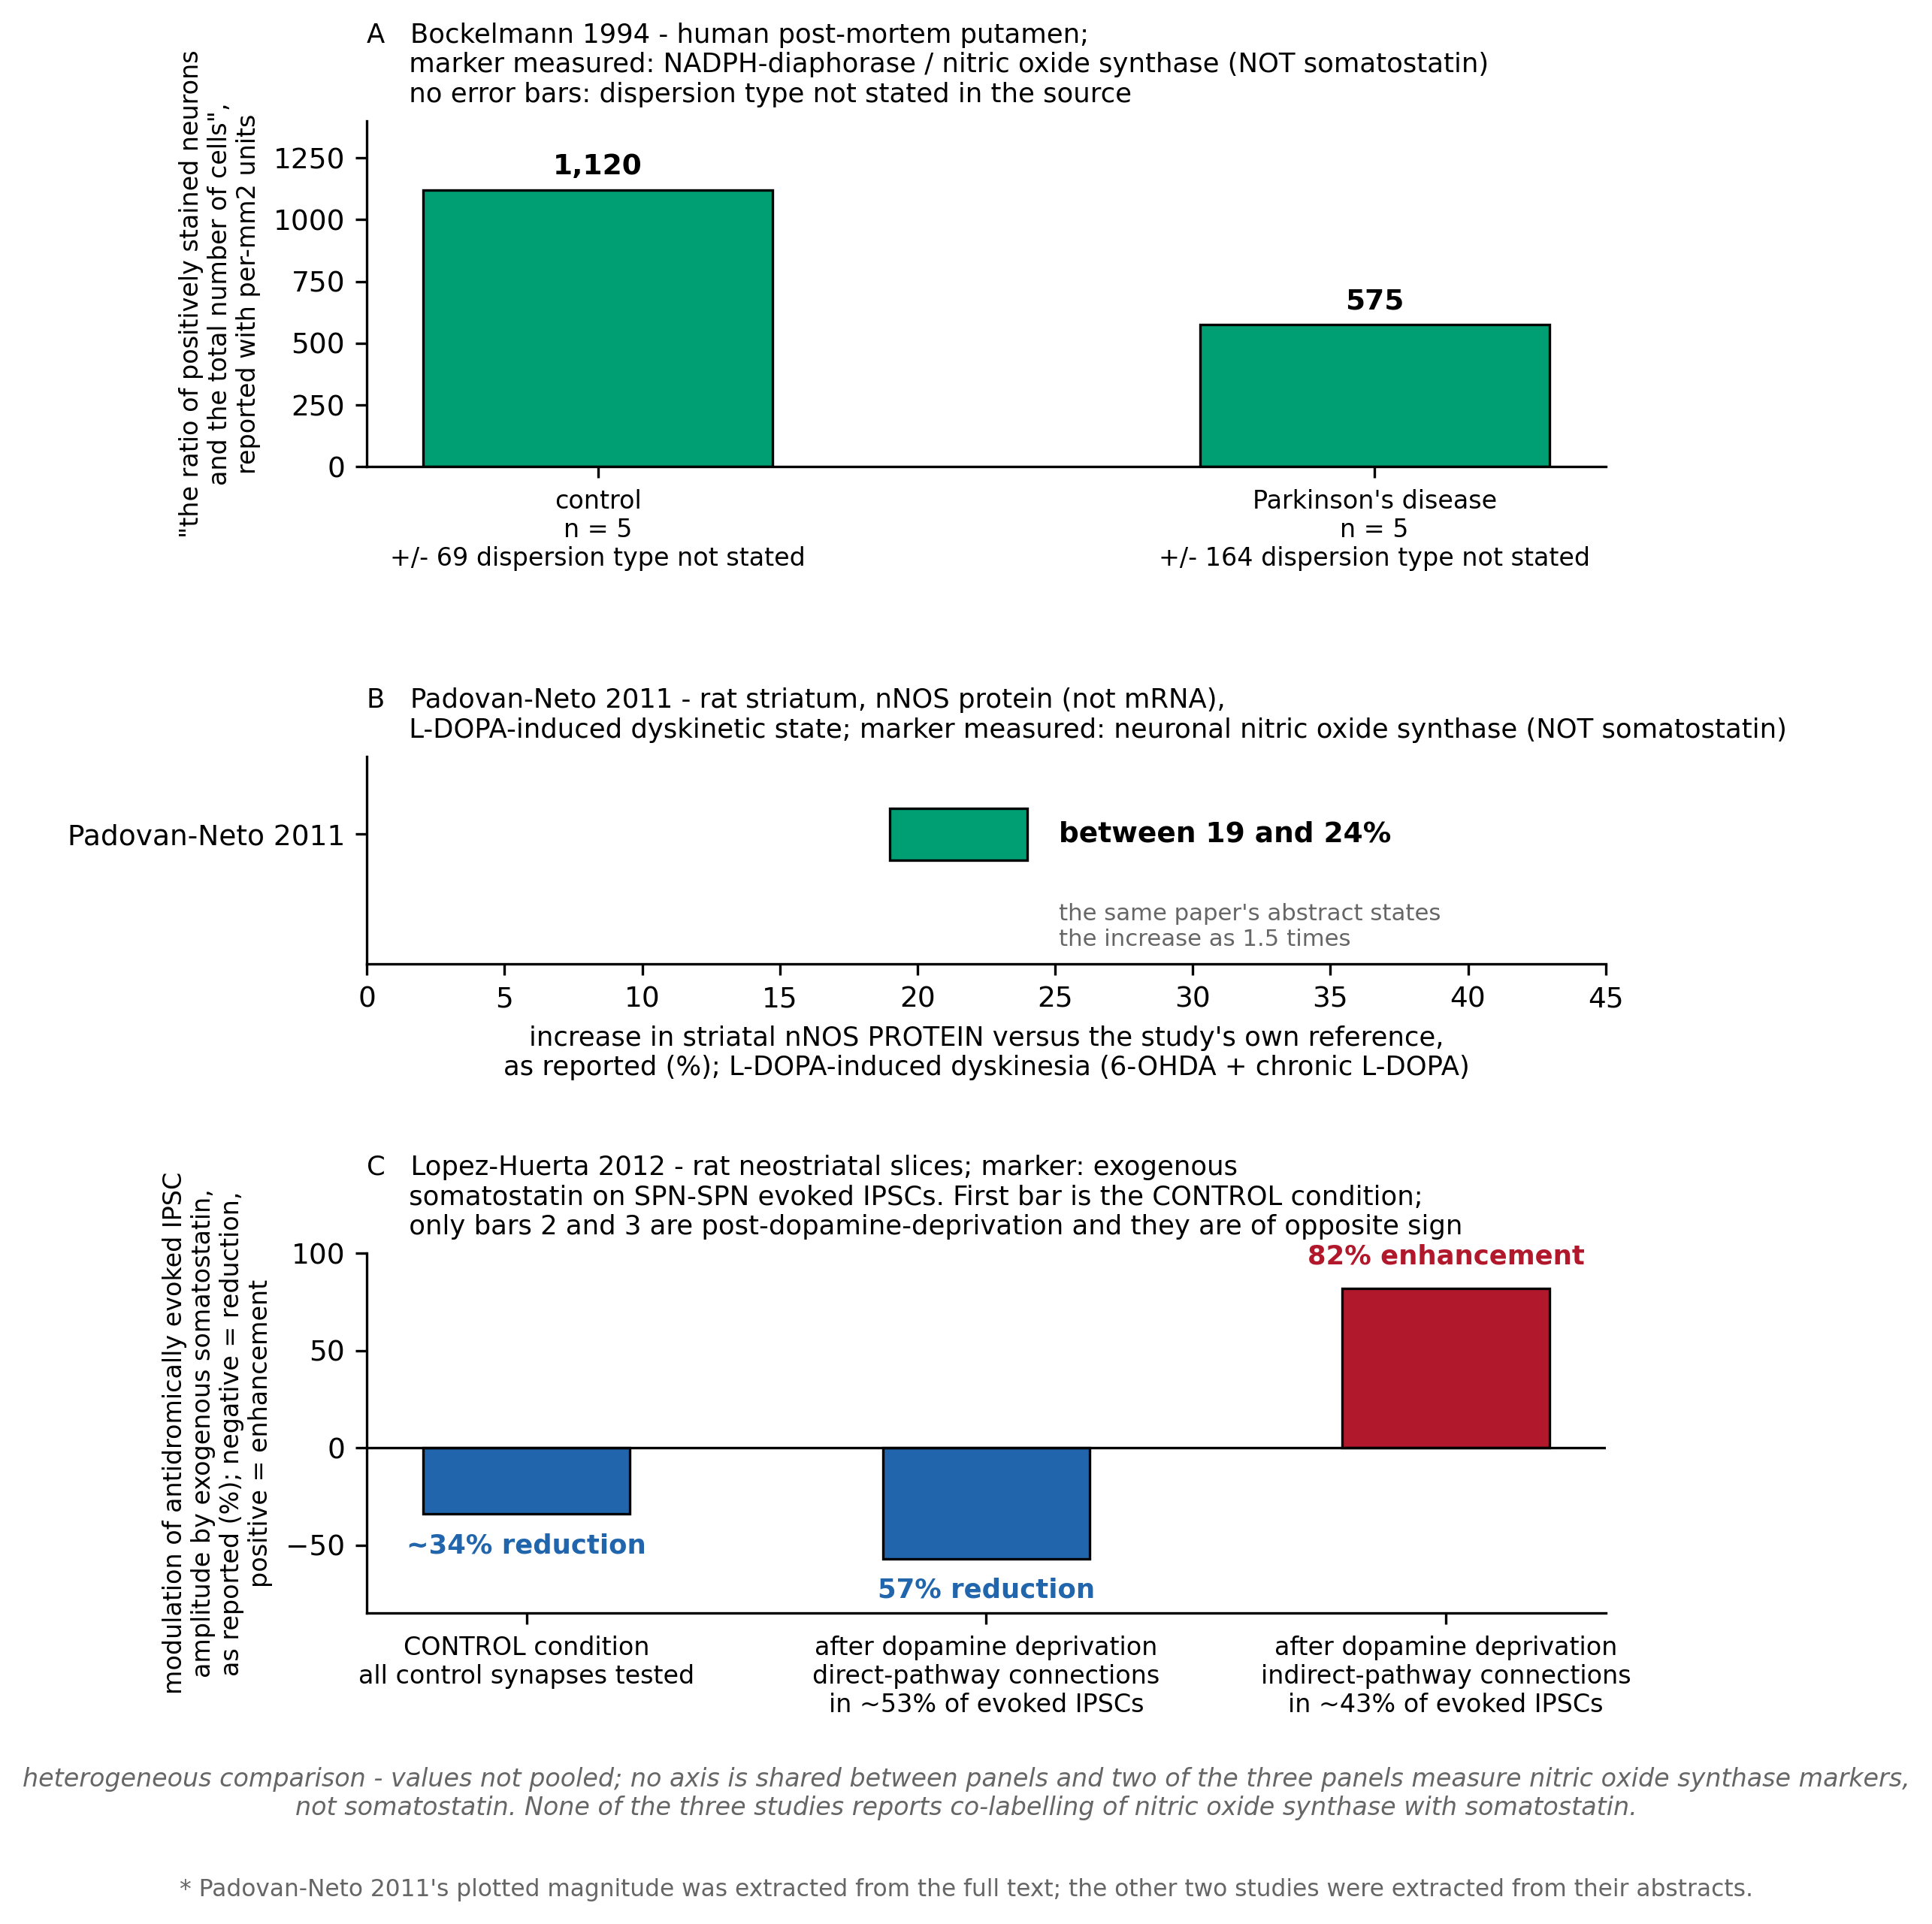
\includegraphics[width=\linewidth]{../figures/fig_sec5_striatal_sst_system_under_dopamine_loss.png}
\caption{\textbf{Three kinds of striatal measurement, three axes.} Each panel carries one study, one marker and its own units; nothing is pooled. Two of the three panels measure nitric oxide synthase markers, not somatostatin: the marker measured is named in every panel title, and none of the three studies reports co-labelling of nitric oxide synthase with somatostatin. No axis is shared between panels: cell density, Western-blot protein abundance and percent modulation of a synaptic current are not interconvertible quantities. Panel A's +/- 69 and +/- 164 are of unstated dispersion type and are printed as text rather than drawn as error bars; the source itself describes the plotted quantity as a ratio of stained neurons to total cells while printing per-mm2 units, and the axis reproduces that wording without resolving it. Panel B is striatal nNOS protein in the L-DOPA-induced dyskinetic state (6-OHDA lesion plus chronic L-DOPA), not dopamine depletion alone and not mRNA; "dorsal" is not stated in the retrieved text, the same study also reports nNOS increases in frontal cortex and a larger mRNA increase in some compartments that are not shown, and the paper gives two conflicting magnitudes for the protein increase (between 19 and 24\% in the full text versus 1.5 times in the abstract), both of which are displayed and neither of which is reconciled. The first bar of panel C is the control condition --- somatostatin reduced IPSCs by \textasciitilde{}34\% in all control synapses tested --- not a post-lesion sub-population; only the 57\% reduction and the 82\% enhancement are post-dopamine-deprivation, and they are of opposite sign, while the fractions of evoked IPSCs affected (\textasciitilde{}53\% and \textasciitilde{}43\%) are printed as annotations, not plotted. Group sizes are reported only for the human entry ("n = 5" control and "n = 5" PD); the rodent entries carry no n or dispersion in the retrieved text. Sources: \citep{Bockelmann1994,PadovanNeto2011,LopezHuerta2012}.}
\label{fig-sec5-striatal-sst-system-under-dopamine-loss}
\end{figure}

\begin{figure}[H]
\centering
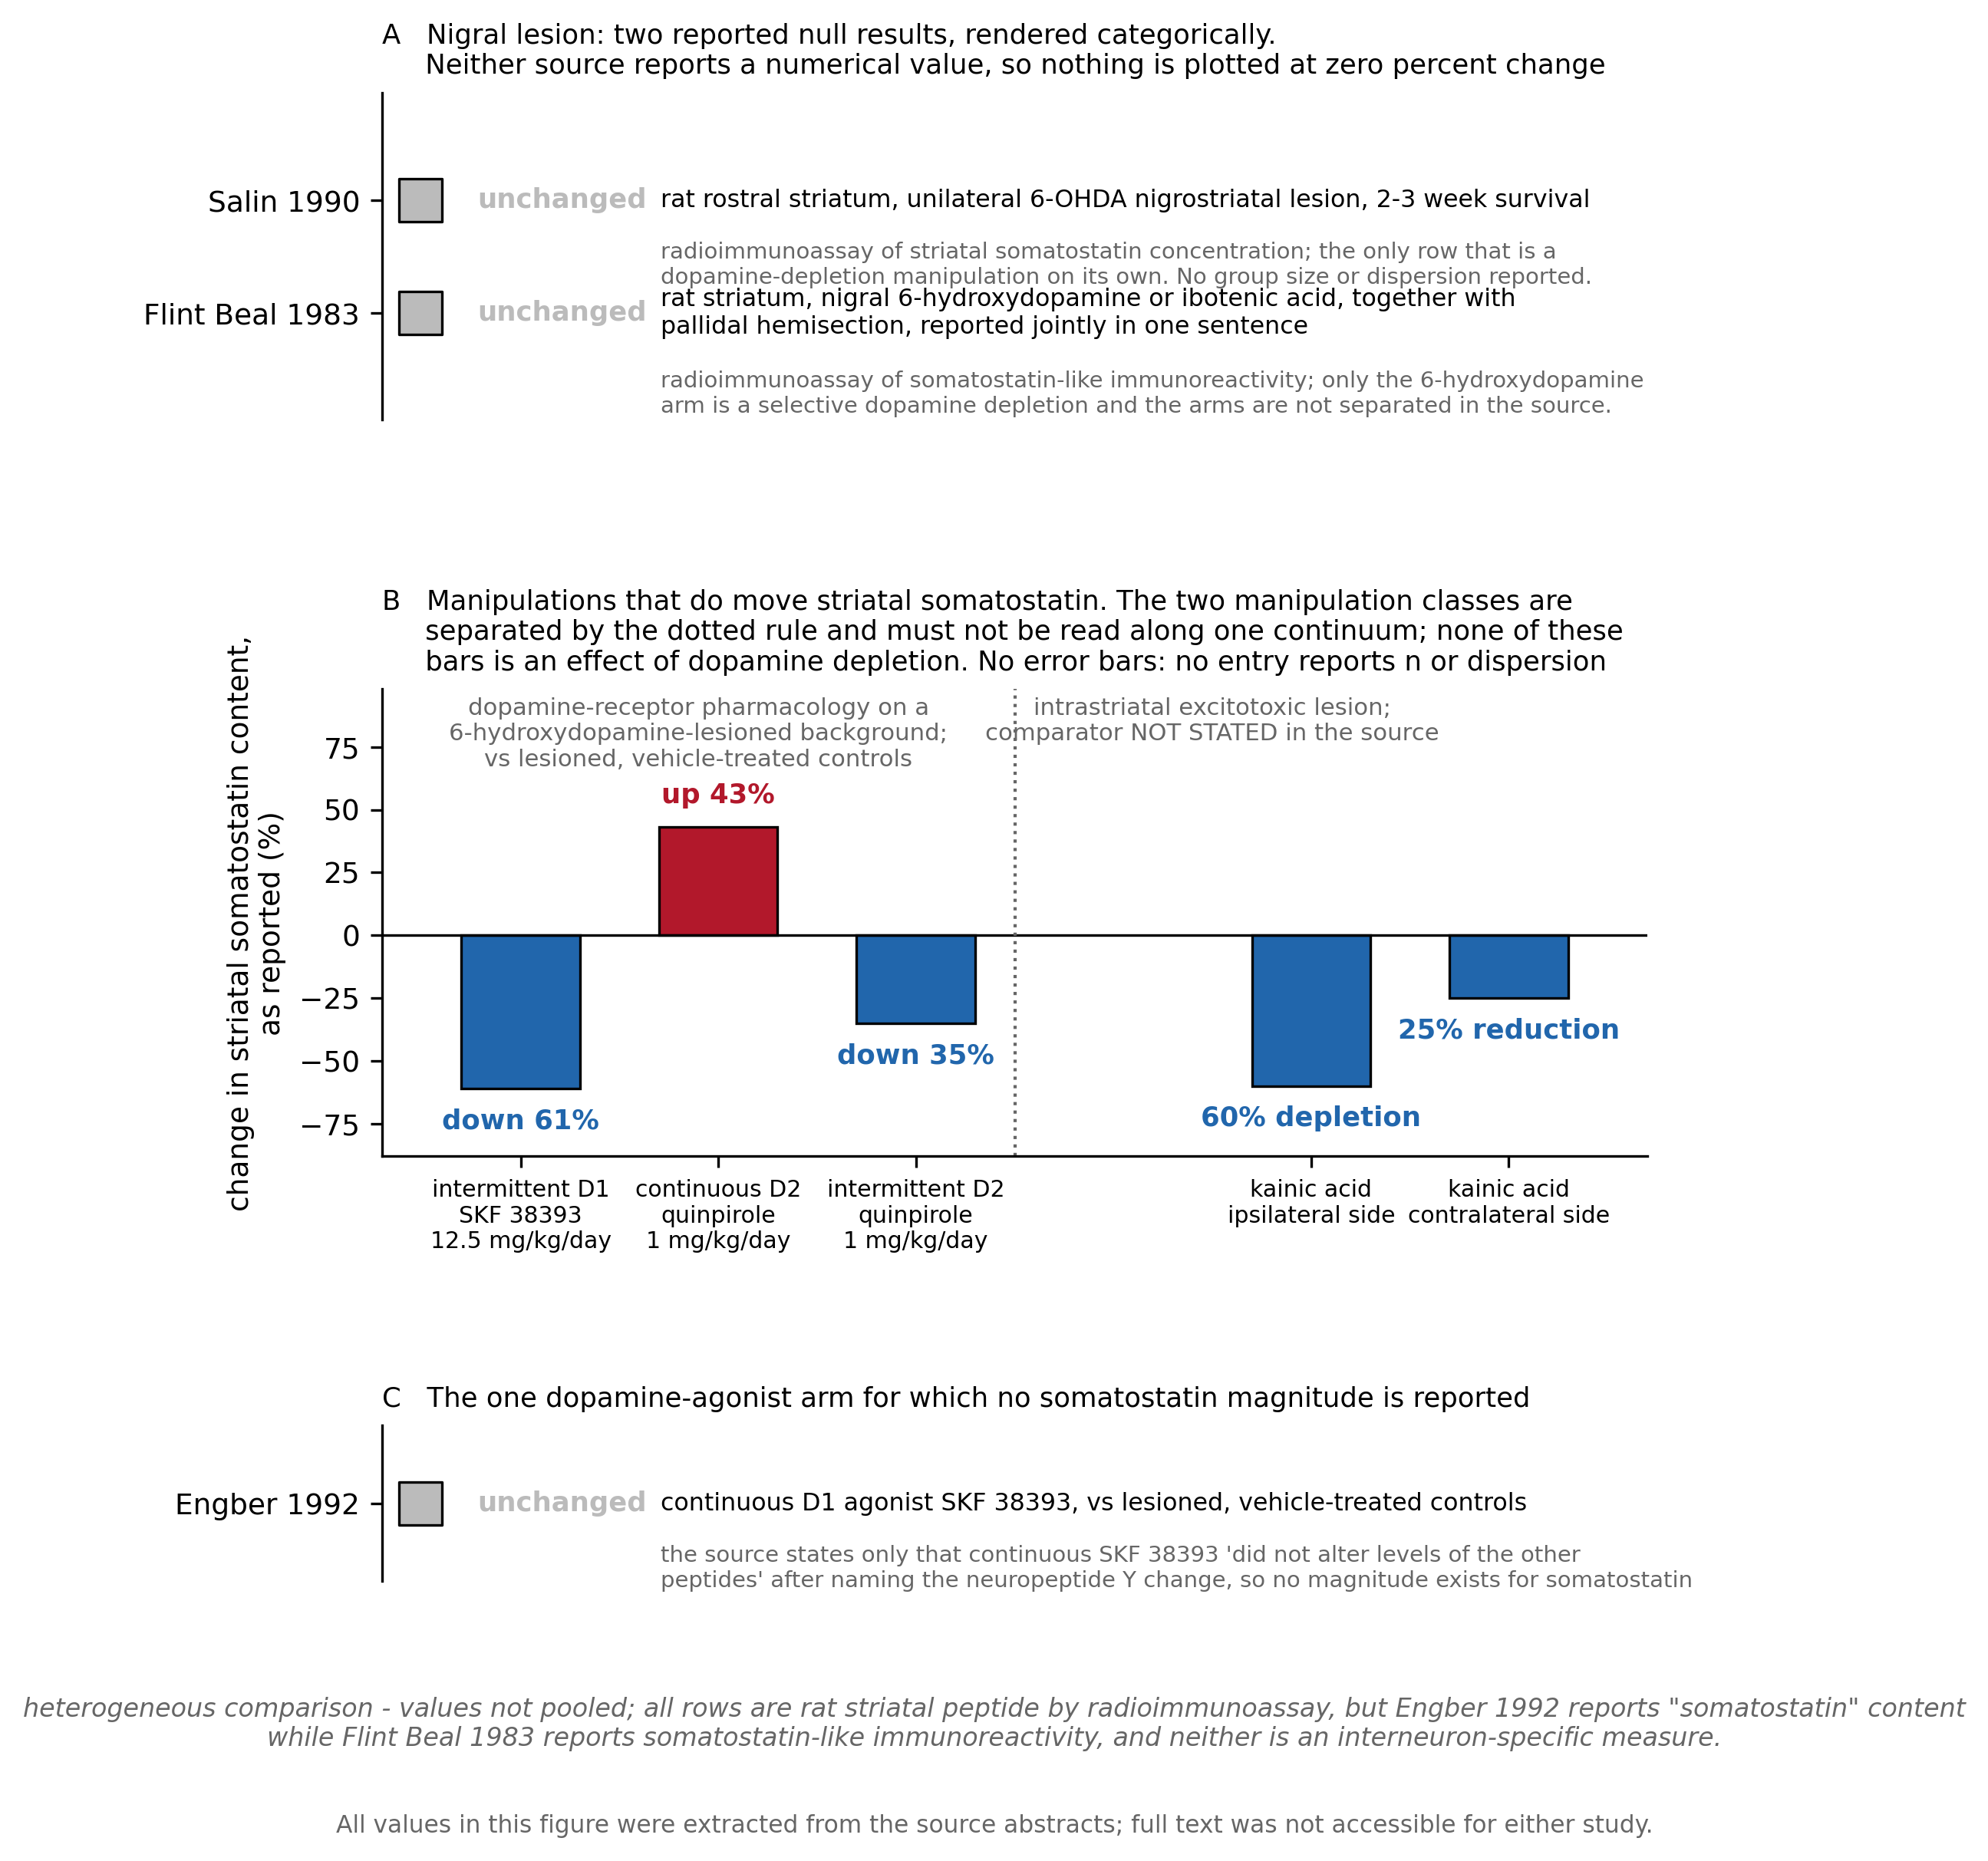
\includegraphics[width=\linewidth]{../figures/fig_sec5_striatal_somatostatin_by_manipulation_class.png}
\caption{\textbf{Striatal somatostatin by class of manipulation.} Panel A holds the two reported null results after nigral lesion; panel B holds the manipulations that do move the peptide; panel C holds the one treatment arm reporting no somatostatin magnitude. Panel A caveats: both rows are categorical outcomes, neither source reports a numerical value, and nothing is plotted at zero percent change; Flint Beal 1983's null covers nigral lesions made with 6-hydroxydopamine or with ibotenic acid, together with pallidal hemisection, in a single reported result, only the 6-hydroxydopamine arm is a selective dopamine depletion, the arms are not separated in the source, and only Salin 1990's row is a dopamine-depletion manipulation on its own; the region is as reported --- rostral striatum in Salin 1990, striatum in Flint Beal 1983 --- and neither source specifies dorsal striatum; both rows are bulk peptide radioimmunoassay, not an interneuron-specific measure, and Flint Beal 1983 concludes that about half of striatal somatostatin-like immunoreactivity is localisable to intrinsic neurons; neither study reports group sizes or dispersion, so these nulls cannot be distinguished from low statistical power. Panels B and C caveats: each bar is labelled by its intervention and its comparator, namely D1 or D2 agonist on a 6-hydroxydopamine-lesioned background measured against lesioned, vehicle-treated controls, and intrastriatal kainic acid for which the source states no comparator; the two manipulation classes are drawn as separated groups and are not on one continuum, because the Engber 1992 bars are drug effects with the 6-hydroxydopamine lesion in the denominator while the kainic-acid bars are effects of the excitotoxic lesion itself, and none of these bars is an effect of dopamine depletion --- the dopamine-depletion result is the null shown in panel A; all four dopamine-agonist arms of Engber 1992 are shown, including the two of opposite sign, because the direction depends on receptor subtype and dosing regimen, and the study reports that alterations in peptide content were observed primarily in the denervated striatum; the contralateral striatum in the kainic-acid study is itself reduced by 25\%, so no unaffected within-animal reference exists for either kainic-acid value; these are bulk peptide measurements, not interneuron-specific, and Flint Beal 1983 concludes that about half of striatal somatostatin-like immunoreactivity is localisable to intrinsic neurons; Engber 1992 reports "somatostatin" content while Flint Beal 1983 reports somatostatin-like immunoreactivity, both by radioimmunoassay, as printed on the rows; no error bars are drawn because no entry in this figure reports a group size or dispersion. Sources: \citep{Salin1990,FlintBeal1983,Engber1992}.}
\label{fig-sec5-striatal-somatostatin-by-manipulation-class}
\end{figure}

\subsection{Alpha-synuclein and interneurons: little inclusion burden, altered function}
\label{sec-05-alpha-synuclein-burden}

If somatostatin interneurons are affected in Lewy body disease, the mechanism is unlikely to be inclusion pathology inside those cells. Three preparations bear on how much alpha-synuclein inhibitory interneurons contain, each with a different denominator: the somatostatinergic share of pathology-bearing cells in olfactory bulb, the share of hippocampal parvalbumin interneurons bearing alpha-synuclein, and baseline expression in cultured GAD-positive neurons. In human olfactory bulb, around 8\% of cells containing Lewy pathology are somatostatinergic, as against more than 50\% of calcium-binding-protein-expressing cells --- a contrast relayed by \citet{SaizSanchez2020} and credited in its own sentence to a primary study that could not be consulted. In DLB hippocampus, \citet{Bernstein2011} found that only 2\% of parvalbumin-expressing interneurons were laden with alpha-synuclein immunoreactive material, yet parvalbumin-immunoreactive neuron density was significantly decreased in dentate/hilus and CA1 with total neuron density preserved. In primary mouse hippocampal culture, \citet{Taguchi2014} quantified that 89$\pm$1.4\% of GAD-positive neurons displayed no expression of alpha-synuclein (6 coverslips were analyzed), and found that those neurons did not form Lewy-body-like aggregates after preformed-fibril treatment unless human alpha-synuclein was exogenously expressed. The denominators of these three numbers are different in kind, which \ref{fig-sec5-alpha-synuclein-interneuron-denominators} makes explicit rather than smoothing. The inference the data support is narrow but important: low inclusion burden coexisting with reduced marker density points to a non-cell-autonomous mechanism --- network, trophic or input-driven --- rather than to direct aggregate toxicity within the interneuron. It is also where the evidence stops. Systematic quantification of Lewy pathology inside identified somatostatin interneurons across cortical regions and Braak stages was not retrieved by these searches, and the available counts are for parvalbumin cells and for olfactory bulb, not for cortical or striatal somatostatin populations.

\begin{quote}
\noindent\textbf{Evidence Conflict}\par
Whether reduced interneuron marker density means fewer interneurons is unresolved and recurs throughout this review. \citet{Bernstein2011} read decreased hippocampal parvalbumin density in DLB as partial interneuron loss; \citet{Schreiber2024} argue from a hamster infection model with alpha-synuclein dysregulation that increases or decreases in parvalbumin- or calretinin-positive counts are unlikely to represent loss or gain of neurons and more likely reflect up- or down-regulation of the calcium-binding protein used to identify them. The same ambiguity has a directional variant: \citet{Radovanovic2021} found an \emph{increased} number of dentate parvalbumin interneurons in rats with cholinergic pedunculopontine lesions, opposite to the human DLB finding, and a reduced dentate parvalbumin number when the nigral and pedunculopontine lesions are combined, so the direction turns on which systems are lesioned; the coupling to sleep-wake architecture belongs to the combined-lesion condition alone, where the reduction in parvalbumin number tracked shorter hippocampal wake episodes (r = 0.52, p = 0.01) and no such relation held in the other groups. \citet{Hawksworth2026} add a regional qualifier, reporting lower parvalbumin interneuron density in DLB cingulate gyrus (t = 2.838, df = 25.86, p = 0.0087) but not inferior temporal gyrus (p = 0.1370), with MAP2-positive neuronal density preserved. None of these studies identifies cells independently of the marker, which is exactly the methodological gap that \ref{sec-conflicts-limitations} treats as a review-wide confound.

\end{quote}

Model systems add a mixed picture rather than a clean one. Alpha-synuclein overexpression does damage interneurons in some preparations --- progressive loss of striatal parvalbumin GABAergic interneurons in SNCA transgenic rats \citep{Paldino2022}, and up to a 50\% reduction of cholinergic interneurons in striatum and cortex after AAV-mediated forebrain overexpression \citep{AldrinKirk2014} --- while in transgenic mouse hippocampus interneuron marker expression was generally unchanged across ages, differing only for calbindin and somatostatin at 43 weeks \citep{FloresCuadrado2016}. Organotypic slice seeding reproduces templated, serine-129-phosphorylated aggregation that spreads between connected hippocampal regions and offers a preparation in which interneuronal transfer can be dissected \citep{Elfarrash2019}. In human anterior olfactory nucleus, somatostatin immunoreactivity in neurites is reduced while parvalbumin is elevated \citep{UbedaBanon2017} --- the same cell-type ordering as the olfactory-bulb pathology-burden shares, although marker level and inclusion burden are different quantities measured in different series. One genetic model suggests a cell-autonomous route after all: GABAergic neurons differentiated from PARK2 patient iPSCs showed significantly reduced SST transcript and fewer somatostatin-positive neurons \citep{Iwasawa2019} --- a single-study observation, unreplicated in seven years, in a monogenic form of the disease. No somatostatin receptor subtype quantification in human parkinsonian or Lewy body tissue was retrieved by these searches, so therapeutic proposals aimed at particular SSTR subtypes in synucleinopathy, discussed in \ref{sec-therapeutics}, currently rest on receptor distributions not measured in the disease tissue in anything these searches returned; the neuroprotective properties attributed to the peptide come from other preparations, including suppression of nigral microglial inflammatory mediators \citep{BAI2015}, Y2-receptor-mediated protection by the co-expressed neuropeptide Y \citep{Decressac2012}, and the general neuropeptide-protection literature summarised by \citet{Behl2022}.

\begin{figure}[H]
\centering
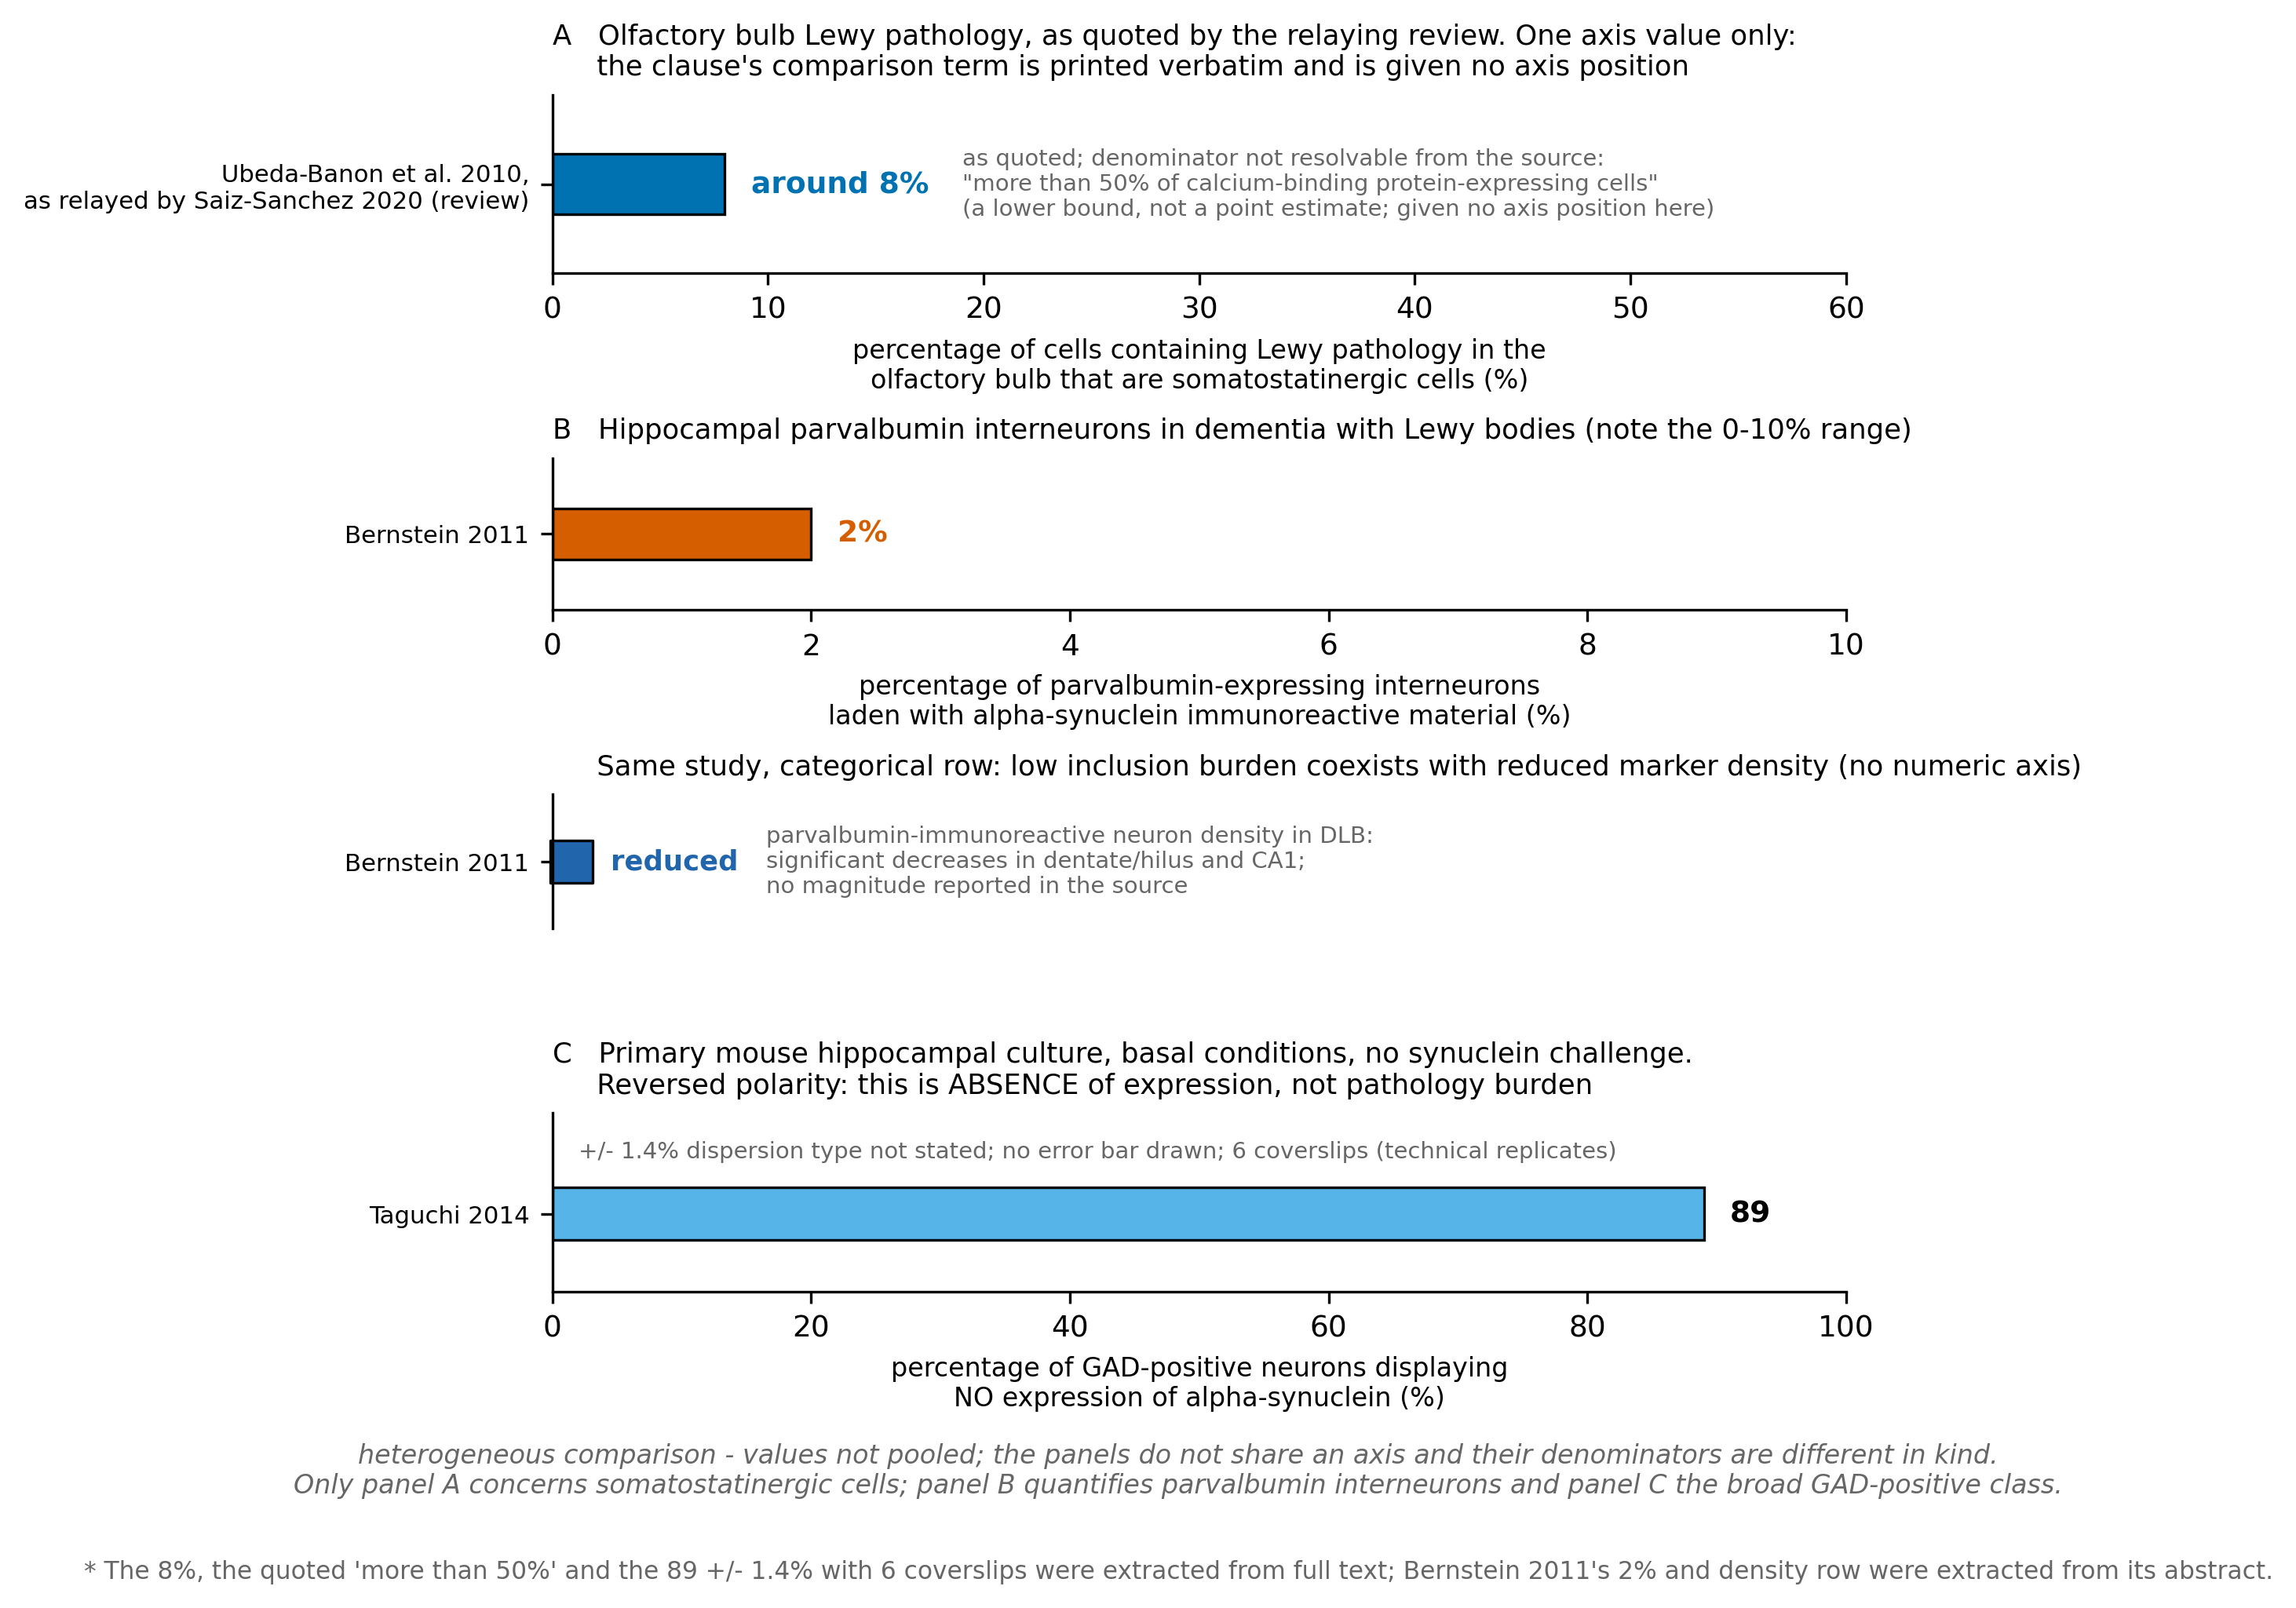
\includegraphics[width=\linewidth]{../figures/fig_sec5_alpha_synuclein_interneuron_denominators.png}
\caption{\textbf{Three percentages, three denominators.} The panels do not share an axis: 8\% is the somatostatinergic share of Lewy-pathology-bearing olfactory bulb cells, 2\% is the share of parvalbumin interneurons bearing alpha-synuclein, and 89\% is the share of cultured GAD-positive neurons with NO detectable alpha-synuclein; each denominator is written into its own axis label. Panel A plots a single value: the source clause's comparison term, "more than 50\% of calcium-binding protein-expressing cells", is printed beside it as a quotation because the clause is ambiguous as to whether that figure shares the 8\% denominator (a share of pathology-bearing cells) or means a burden within the calcium-binding-protein class, and the primary study it credits could not be consulted, so the figure asserts neither reading and plots neither; "more than 50\%" is in any case a lower bound, not a point estimate. The olfactory bulb values are credited by their own source sentence to a primary study of 2010 and are relayed by a short review; case numbers, bulb subregion and co-labelling protocol are unavailable. Low inclusion burden does not imply preserved cells: the same hippocampal study reports significant decreases in parvalbumin-immunoreactive neuron density in the dentate/hilus region and CA1 alongside a 2\% inclusion burden, shown as the categorical row immediately beneath the 2\% bar. Panel C is a baseline-expression measurement in primary mouse hippocampal culture under basal conditions with no synuclein challenge --- mouse, not rat --- and reports absence of expression, not pathology burden; the same study reports that GAD-positive neurons did not form Lewy-body-like aggregates after preformed fibrils but did when human alpha-synuclein was exogenously expressed; its +/- 1.4\% is of unstated dispersion type and is printed as text rather than drawn as an error bar, and its n of 6 is coverslips, i.e. technical replicates. Only panel A concerns somatostatinergic cells; panel B quantifies parvalbumin interneurons and panel C the broad GAD-positive class, in which parvalbumin and somatostatin cells were identified only qualitatively. Olfactory bulb and hippocampus are different regions whose pathology loads are not measured in the same series, so panels A and B cannot be read as a cell-type vulnerability contrast. Neither human entry reports case numbers. Sources: \citep{SaizSanchez2020,Bernstein2011,Taguchi2014}.}
\label{fig-sec5-alpha-synuclein-interneuron-denominators}
\end{figure}

\subsection{L-DOPA, dyskinesia and cognitive decline}
\label{sec-05-ldopa-dyskinesia}

Treatment is both a confound and a phenomenon, and cohorts that mix the two cannot be compared. Chronic L-DOPA alters the peptidergic and nitrergic readouts directly: it raises whole-brain somatostatin while lowering neuropeptide Y in cortex, hippocampus and striatum \citep{Maeda1993}, normalises the late striatal somatostatin deficit seen after MPTP while itself lowering cortical somatostatin \citep{Asanuma1990}, and in the dyskinetic state raises striatal neuronal nitric oxide synthase (nNOS) protein between 19 and 24\% with a ten-times larger increase in nNOS mRNA in the striatum contralateral to the lesion, while nitric oxide synthase inhibition reduces abnormal involuntary movements \citep{PadovanNeto2011}. Because nNOS is expressed by the somatostatin/NPY interneuron class, as set out in \ref{sec-sst-identity}, and by other sources, that therapeutic effect does not identify its causal cell type, and the evidence gap recorded for this literature --- no cell-type-specific manipulation isolating striatal somatostatin interneurons during dyskinesia --- has only just begun to close: \citet{Stahl2026} report increased c-Fos in striatal somatostatin interneurons during L-DOPA-induced dyskinesia and show that chemogenetic inhibition modestly but consistently exacerbates dyskinesia selectively during the wearing-off phase, without altering the antiparkinsonian response. That is one abstract-level study, not a replicated finding. Around it, the dyskinetic striatum shows cholinergic interneurons whose calcium events the authors report as about 50\% larger, which they read as the in vivo counterpart of a bursting-like phenotype seen in slices \citep{Atamna2025}, perineuronal-net remodelling around parvalbumin interneurons in dorsolateral striatum and M1 \citep{Bilbay2025}, and dopamine-receptor-subtype-dependent swings in peptide content \citep{Engber1992}. That some of this remodelling is dopamine-dependent and pharmacologically reversible is shown in hippocampus, where midbrain dopamine loss destabilises perineuronal nets and tissue plasminogen activator around parvalbumin interneurons and D2/D3 receptor activation restores net integrity and inhibitory drive \citep{Cauzzi2026}. Medication also moves peripheral measures: serum somatostatin rises significantly after starting antiparkinson therapy in patients who experience nausea or vomiting \citep{Shiraishi2010}, so treated and de novo cohorts differ at least in peripheral peptide; whether medication shifts cerebrospinal fluid somatostatin was not measured in any series retrieved here.

The cognitive end of the syndrome is where the cortical and striatal stories meet, and the interneuron evidence there is thinner than the peptide evidence. Plasma neuropeptide Y is reported lower in Parkinson's disease than in healthy controls and to decline stepwise with cognitive impairment, lowest in PDD \citep{Zhang2026b} --- a single recent cohort, unreplicated --- while CSF neuropeptide Y is higher in depressed parkinsonian patients than in major depressive disorder \citep{Svenningsson2017}, indicating that peripheral and central peptide measures are not reading the same variable. Functional cortical evidence points to somatostatin interneurons as participants rather than casualties: somatostatin interneuron somatic activity in motor cortex falls within an hour of MPTP and driving those interneurons rescues spine loss and motor deficits \citep{Chen2019}, subthalamic deep brain stimulation activates motor-cortex somatostatin interneurons while inhibiting parvalbumin interneurons and pyramidal cells, with direct optogenetic activation of the somatostatin population alone relieving motor symptoms \citep{Valverde2020}, and cortical inhibitory dynamics and their neuromodulation are altered after dopamine loss in rodents \citep{Minetti2025,Gui2010} and in people assessed with directionally selective transcranial magnetic stimulation \citep{OFarrell2026}. Parkinson-spectrum specificity is suggested by the finding that somatostatin concentrations were normal in every region tested in progressive supranuclear palsy despite reduced choline acetyltransferase \citep{Epelbaum1987}, and by the nigral somatostatin \emph{increase}, not decrease, seen after MPTP in mice \citep{Radke1987}; lesioning also shifts the biotransformation of somatostatin and other precursors rather than simply depleting them \citep{Nilsson2009}. Two further gaps should be stated plainly: no head-to-head quantification of cortical and CSF somatostatin in DLB and PDD within a single cohort and one assay was retrieved, so the two syndromes have no biochemical separator in this record; and no cortical or striatal somatostatin-specific inclusion count was retrieved by these searches, so the non-cell-autonomous inference above is untested here.

These conclusions are bounded by how the literature was assembled. Retrieval was dominated by one biomedical full-text index with no citation chasing, so no claim of complete coverage is made and statements of absence are statements about what these searches returned. Only a minority of the parkinsonian literature here was available as full text --- the 1980s and 1990s radioimmunoassay and cerebrospinal fluid series are recorded at abstract level --- which is why this section quotes source sentences and declines to recompute percentages, convert units or pool values. Searches for disconfirming results were capped, so the reported nulls are a top-relevance sample rather than a census and the rate of contradiction is bounded below, not estimated.

The parkinsonian picture that survives these constraints is of a peptidergic system responding to an altered network state rather than dying: cortical somatostatin falls where Alzheimer-type pathology and dementia are present and not otherwise, striatal somatostatin is unmoved by denervation itself while its synaptic action is reconfigured, and, where inclusion burden has been counted at all --- olfactory bulb somatostatinergic cells and hippocampal parvalbumin cells --- the cells carry few inclusions. The cross-disease direction-of-change contrast set out in \ref{sec-selective-vulnerability} is instantiated here in its sharpest form: the same cell class reads as deficient in cortex, as upregulated in basal ganglia transcript, and as unchanged in rodent striatal peptide, depending entirely on what was measured. \ref{sec-huntingtons} presents the extreme version of that idea --- a striatal interneuron population long described as spared while its projection-neuron targets are destroyed --- and asks whether the sparing claim survives modern measurement.

\section{Huntington's Disease and Striatal SST Interneurons}
\label{sec-huntingtons}

Dopamine depletion leaves the striatal peptidergic system altered but alive, as set out in \ref{sec-parkinsons-lewy-body}; Huntington's disease (HD) poses the complementary question: what becomes of this interneuron class when its postsynaptic targets are destroyed around it.

\subsection{The sparing claim and its measurement basis}
\label{sec-06-sparing-claim}

The textbook answer is that it is spared. That answer traces to a specific and narrow measurement base. Postmortem HD striatum contains two- to threefold higher somatostatin and NPY concentrations than control tissue, an increase the original reports attributed partly to striatal atrophy \citep{Beal1991b}; peptide increases of similar size in mild and severe neuropathological grades were read by those authors as consistent with a relative but not absolute sparing of the aspiny neurons in which somatostatin and NPY are colocalised \citep{Beal1988}. Elevated NPY in cerebrospinal fluid is measured directly in HD cohorts \citep{Wagner2016}, while the higher NPY-positive neuron counts in the HD caudate-putamen reach this literature as a restatement inside a later spatial-transcriptomic study rather than as a primary count retrieved here \citep{Burns2025}, and in primate excitotoxin models GABA and substance P immunoreactivity fall while somatostatin-like, NPY-like and choline acetyltransferase immunoreactivity show no significant depletion \citep{Ferrante1993}. The canonical syntheses state the position compactly: spiny projection neurons and parvalbumin interneurons degenerate progressively while cholinergic and nitric oxide synthase (NOS)-containing interneurons are relatively spared \citep{Morigaki2017}, the NADPH-diaphorase-positive cells reportedly even at late stages \citep{Mitchell1999}.

Three features of that base deserve stating plainly. First, peptide concentration is normalised to tissue that is itself shrinking, so an unchanged number of peptide-containing cells in a smaller striatum yields a concentration increase --- which the report of the two- to threefold rise named as a possible cause \citep{Beal1991b}, while the companion grade analysis drew the relative-sparing reading from the similarity of the increases across grades \citep{Beal1988}. Second, the histochemical arm of the claim rests on NADPH-diaphorase staining \citep{Brouillet1995,Beal1993}, a readout that reports the presence of the marker and therefore cannot by itself separate surviving cells from functionally intact ones. Third, and most consequentially, a primary demonstration of absolute sparing using modern cell-type-specific markers with unbiased stereology was not retrieved by these searches; the quantitative counts that do exist come from mouse models and do not agree with each other, one reporting small marker-positive reductions \citep{Rajput2011} and the other no significant change in striatal somatostatin interneuron number \citep{Rallapalle2021}. The claim that striatal interneurons are spared in HD is therefore repeated far more confidently than its primary data support, and the excitotoxicity literature on which it was originally built, treated in \ref{sec-selective-vulnerability}, was never designed to settle cell number. Forty of the eighty reports underlying this section were available as full text; the 1980s and 1990s peptide and radioimmunoassay series carrying much of the sparing claim is represented here by abstracts only, an asymmetry that falls precisely on the historical foundation of the argument.

\subsection{Peptide up, transcript down: the dissociation inside the spared population}
\label{sec-06-peptide-transcript}

The sharpest internal evidence against reading sparing as integrity comes from putting peptide and transcript measurements side by side in the same region. In situ hybridisation in human HD brain found neuronal nitric oxide synthase mRNA significantly decreased in caudate nucleus and putamen but not in sensorimotor cortex, with the decrease becoming more pronounced as neuropathological severity increased \citep{Norris1996}. That is the same striatum in which somatostatin and NPY peptide concentrations rise \citep{Beal1988,Beal1991b}. Transcript loss that tracks severity inside a population whose peptide content rises is what one expects of surviving cells with downregulated transcription in atrophic tissue, not of a population unaffected by the mutation. The same picture appears in other molecular readouts of this class: cannabinoid CB1 receptor expression is downregulated in striatal NPY/nNOS-expressing interneurons in R6/2 mice, in Hdh(Q150/Q150) mice and in human HD caudate \citep{Horne2012}, cannabinoid receptor loss in R6/1 mice is concentrated in hippocampal GABAergic interneurons, where it is the likely cause of impaired depolarisation-induced suppression of inhibition in a different interneuron population from the striatal class at issue here \citep{DiFranco2025}, cholinergic interneurons and astroglia in HD knock-in mice downregulate a large set of projection-neuron marker genes \citep{Lee2020}, and surveys of striatal nuclei report bidirectional dysregulation of cell-type-specific gene networks, with altered signalling probability for the NPY/SST interneuron cluster itself \citep{Malaiya2021,Jiang2024}. The receptor system through which somatostatin signalling might protect these cells is itself coupled to that remodelling: co-activation of somatostatin receptors with CB1 abolishes the protection that somatostatin receptor activation confers in huntingtin knock-in striatal cells \citep{Zou2019}.

\begin{quote}
\noindent\textbf{Evidence Conflict}\par
\textbf{Peptide concentration versus transcript level in the same region.} Radioimmunoassay of HD striatum reports increased somatostatin and NPY, read as relative sparing of the cells that contain them \citep{Beal1988}; in situ hybridisation of the same region reports significantly decreased nNOS mRNA that worsens with grade \citep{Norris1996}. The disagreement is not about which result is correct but about what each measures --- peptide content normalised to atrophic tissue versus per-neuron transcript --- and it is resolved by that distinction rather than by new data. Both are compatible with surviving but transcriptionally downregulated cells, and neither establishes functional integrity.

\end{quote}

The excitotoxic provenance of the sparing claim is also less unanimous than its repetition suggests. Injection of N-methyl-D-aspartate (NMDA)-type agonists into rat dorsolateral frontoparietal cortex reduces glutamate and GABA markers while somatostatin, NPY, substance P, cholecystokinin and VIP are unchanged or increased \citep{Beal1991a}, and the sparing is agonist-specific: kainate, quisqualate and AMPA produce dose-dependent reductions in all four markers examined, which is the basis of the inference that resistance reflects a paucity of NMDA receptors rather than general excitotoxic resistance \citep{Beal1989}. In culture, striatal neurons containing either NADPH-diaphorase or acetylcholinesterase are more resistant to NMDA and quinolinate than the general striatal population, though the resistance is not absolute and is overcome by intense exposure; heightened vulnerability to kainate is confined to the NADPH-diaphorase-containing neurons and is not shown by the acetylcholinesterase-containing ones \citep{Koh1988}. Against this, a stereological study of intrastriatal quinolinic acid lesions found parvalbumin- and NPY-positive interneuron numbers significantly reduced relative to control in the peri-lesional transition zone, reported as a test statistic without an effect-size magnitude \citep{Feng2014}, and an earlier comparison, represented here only by its abstract, states that the preservation of somatostatin/NPY/NADPH-diaphorase-containing neurons found in HD was not observed following quinolinic acid lesions \citep{Davies1988}. The one pharmacological test of the obvious mechanistic candidate retrieved here was negative: systemic NOS inhibition neither protected against nor potentiated quinolinic-acid-induced loss of NADPH-diaphorase, NOS or acetylcholinesterase neurons \citep{Mackenzie1995}.

Candidate determinants of the differential outcome remain correlational and scattered across preparations. nNOS-positive striatal neurons show no detectable mitochondrial reactive oxygen species rise on NMDA receptor activation while nNOS-negative neurons do, although the same report records a further set of experiments in which no difference between nNOS-positive and nNOS-negative striatal neurons was observed \citep{Canzoniero2013}; group I metabotropic glutamate receptor activation depolarises large aspiny cholinergic interneurons without affecting spiny neuron membrane properties \citep{Calabresi1999}; and huntingtin protein itself is distributed unevenly, with little or no huntingtin immunoreactivity in choline acetyltransferase-, parvalbumin-, calretinin- or nNOS-positive interneurons in one survey \citep{Kosinski1997} but concentration \emph{in} striatal interneurons, and detectable huntingtin message in only about 65\% of projection neurons, in another \citep{Fusco1999}, against a background of topographically and cellularly heterogeneous huntingtin immunoreactivity in human neostriatum \citep{Ferrante1997}. For three further mechanistic proposals in this literature, no independent replication was retrieved by these searches in the fourteen to thirty years since publication: that somatostatin itself is the feature conferring sparing under excitotoxicity \citep{Kumar2008}, that optineurin is abundant in striatal interneurons and low in projection neurons in a pattern complementary to HD loss \citep{Okita2012}, and that huntingtin-associated protein 1 mRNA is co-enriched with nNOS mRNA in discrete neuronal populations \citep{Li1996a}. No study manipulating one of these candidates and measuring interneuron survival in a genetic HD model was retrieved by these searches, so the mechanism of the differential outcome is, at present, an inference from correlations gathered across decades and preparations.

\subsection{Sparing relative to what: the parvalbumin contrast}
\label{sec-06-parvalbumin-contrast}

Sparing is in any case a comparative statement, and the comparison class matters. Parvalbumin interneurons carry the most consistent loss evidence in the striatum: reduced per-area density in the dorsal striatum of 12--14-month BACHD mice where somatostatin-positive interneuron numbers in the same animals at the same stage are unchanged \citep{Rallapalle2021}, major count reductions in the caudate nucleus of two transgenic HD macaques \citep{Lallani2019}, markedly reduced density with somatic atrophy in R6/2 striatum \citep{Paldino2017}, and significant reduction after excitotoxic lesion \citep{Feng2014}. In cortex the picture divides rather than converges: severe loss in the human anterior cingulate cortex of mood-dominant HD cases \citep{Kim2014} sits against unchanged parvalbumin density in R6/2 cortex and unchanged parvalbumin counts in BACHD cortex at the stage measured \citep{Voelkl2022,Molero2026}, and cortical GABA-release deficits have been produced in one model without any loss of parvalbumin interneurons at all \citep{Dougherty2014}. The clinical reading of that class --- that parvalbumin interneuron loss may contribute to late dystonia and rigidity --- is itself a proposal rather than a demonstration \citep{Reiner2018}. \ref{fig-sec6-sst-sparing-versus-pv-loss-hd} places the somatostatin and parvalbumin measures on the same page, and the exercise exposes how unlike each other the underlying measurements are: an area-normalised density, a percent marker reduction, a raw count on a study's own scale and a soma-size morphometric cannot be read as one series, and the parvalbumin evidence spans a mouse, a monkey, a human cortex and a rat lesion in three different units, with only the monkey and the human measures sharing a reporting convention.

\begin{figure}[H]
\centering
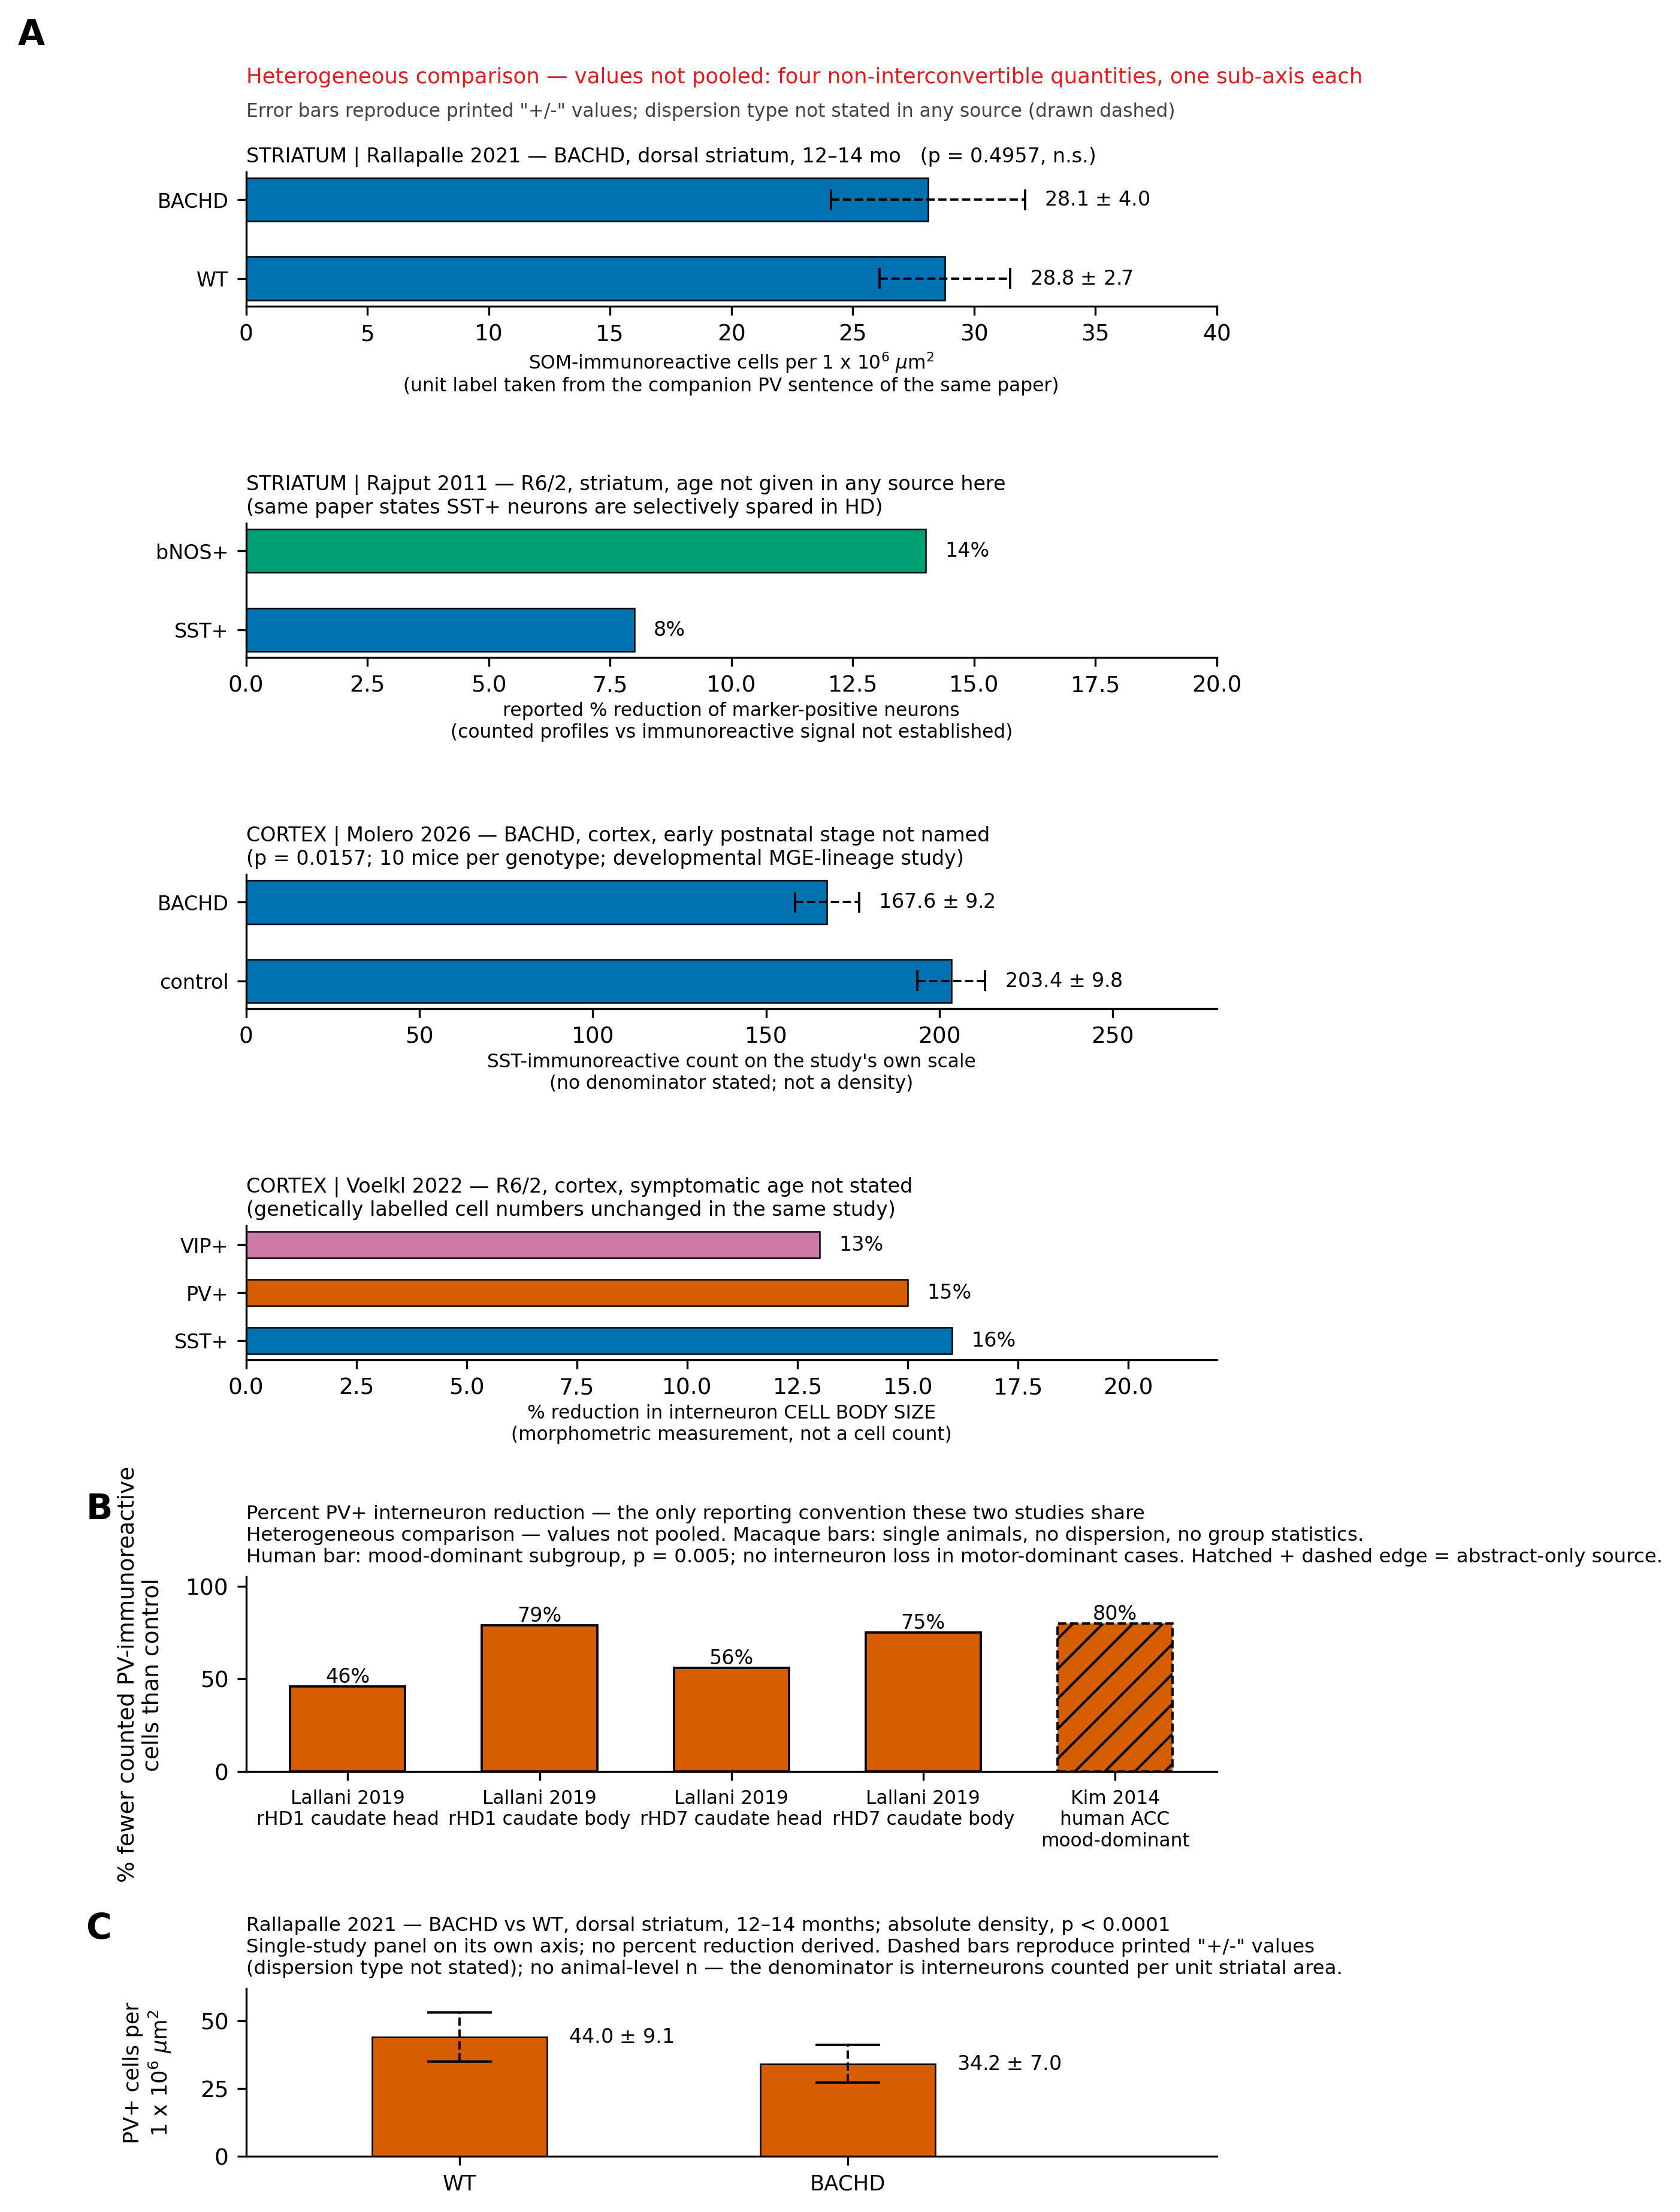
\includegraphics[width=\linewidth]{../figures/fig_sec6_sst_sparing_versus_pv_loss_hd.png}
\caption{\textbf{Somatostatin and parvalbumin interneuron measures in Huntington's disease.} (A) Four single-study rows, each on its own sub-axis with its own unit, blocked striatum (rows 1--2) then cortex (rows 3--4). The four quantities --- area-normalised SOM-immunoreactive number, percent reduction of marker-positive neurons, cortical SST-immunoreactive counts on the study's own scale, and percent reduction in interneuron cell body size --- are not interconvertible and must not be read as one series; no pooled or averaged effect is shown or implied \citep{Rallapalle2021,Rajput2011,Molero2026,Voelkl2022}. Row 4 is a cell-body-size measurement, not a cell count, and is labelled as such in the table body. In R6/2 cortex reduced somatostatin immunoreactivity coexists with unchanged genetically labelled cell numbers, indicating loss of molecular marker rather than loss of cells \citep{Voelkl2022}; for the R6/2 striatal row that study's report does not establish whether the 8\% and 14\% figures are counted profiles or immunoreactive signal, so they are described neither as counted-profile losses nor as demonstrated cell death, and that same paper's stated position is that somatostatin-positive neurons are selectively spared in HD \citep{Rajput2011}. Stages are not comparable and not all stated: 12--14 months for the BACHD striatal row, an unnamed early postnatal stage for the BACHD cortical row (whose source reports reduced cortical somatostatin-positive interneurons at PND13 and persistence at PND30) and an unstated symptomatic age for the R6/2 cortical row, while no age for the R6/2 striatal row is given in any source available here. The BACHD cortical value comes from a developmental medial ganglionic eminence lineage study rather than an adult degeneration time course, and its sample size is reported as 10 mice per genotype \citep{Molero2026}. R6/2 is an exon-1 fragment model and BACHD a full-length BAC transgenic model; the two differ in aggressiveness and onset. The cortical somatostatin-immunoreactive counts (203.4 control versus 167.6 BACHD) come from the developmental cortical study and are reported without a stated denominator, so that axis is a count on that study's own scale and not a density \citep{Molero2026}; the BACHD striatal row carries the unit under which its source reports striatal interneuron counts, SOM-immunoreactive cells per 1 $\times$ 10$^{6}$ $\mu$m$^{2}$ of striatal area, the label being taken from the companion parvalbumin sentence of that paper \citep{Rallapalle2021}. Error bars reproduce the "$\pm$" values exactly as printed in each study's report; the sources state neither standard deviation nor standard error, so bars are drawn dashed and are not comparable between rows, and n denominators differ (one study reports 10 mice per genotype, the others report counted objects or state no n). (B) Percent reduction in counted parvalbumin-positive cells versus control, the only reporting convention these two studies share; species and region differ (transgenic rhesus macaque caudate nucleus, human anterior cingulate cortex), the pairing is descriptive rather than a progression, and no pooled or meta-analytic estimate is computed. The human 80\% value applies to HD cases with a dominant mood phenotype and carries p=0.005 in its source; the same study found no interneuron loss in the anterior cingulate cortex of motor-dominant cases, and in primary motor cortex only calbindin interneurons were lost, while the companion 71\% calbindin and 60\% calretinin losses in the same sentence carry p=0.001 and are not plotted here \citep{Kim2014}. The macaque bars are values from two animals reported individually (rHD1: 46\% head, 79\% body; rHD7: 56\% head, 75\% body) with no dispersion and no group-level statistics; in the same study striatal volume was reduced only in rHD1 and overall interneuron density was increased in rHD1, which that report reads as relative sparing of interneurons over projection neurons \citep{Lallani2019}. Only the human study used double-blind design-based stereology, with 13 HD cases and 15 matched controls and the mood-dominant subgroup size not stated. Striatal and cortical parvalbumin-expressing interneurons are distinct cell classes: the shared axis reflects a shared reporting convention, not one population measured twice, the bars are not repeated observations of one quantity, and no count of studies or animals can be read off the axis. (C) Rodent parvalbumin data are plotted separately because the quantity is an absolute per-area density (BACHD, 12--14 months, dorsal striatum), from which no percent reduction is derived; error bars reproduce the printed "$\pm$" values and the source does not state whether they are standard deviations or standard errors, and the bars carry no animal-level n, the denominator being interneurons counted per unit striatal area \citep{Rallapalle2021}. The rat quinolinic acid result is a test statistic only (Parv+ F = 40.717 and NPY+ F = 22.846, df1 = 2, df2 = 12, both p<0.01) and is not plotted: it carries no effect-size magnitude, it is an acute excitotoxic lesion rather than a mutant-huntingtin model, and its counts are restricted to the peri-lesional transition zone \citep{Feng2014}. No animal-level n is reported for that study in any available source, and the number of experimental units behind its degrees of freedom is not given and is not inferred.}
\label{fig-sec6-sst-sparing-versus-pv-loss-hd}
\end{figure}

Within the mouse literature the quantitative disagreement is small but real, and it lines up with construct. R6/2, an exon-1 fragment model, yields reported reductions of 14\% and 8\% in brain nitric oxide synthase- and somatostatin-positive striatal neurons \citep{Rajput2011}, while BACHD, a full-length transgenic, yields no significant change in somatostatin-positive interneuron number in the same region \citep{Rallapalle2021}. The two can be reconciled by model aggressiveness rather than by discarding either, and the same construct dimension organises much of the disagreement in this field, as \ref{sec-conflicts-limitations} sets out. What neither study establishes is whether the quantity measured is a count of cells or of immunoreactive profiles --- a distinction that is not a technicality here, because in R6/2 cortex reduced somatostatin and VIP immunoreactive density coexists with unchanged genetically labelled cell numbers for all interneuron types, which the authors read as loss of molecular marker in the absence of cell death \citep{Voelkl2022}.

\subsection{Functional pathology in a surviving population}
\label{sec-06-functional-pathology}

If sparing means survival rather than integrity, the physiological measurements should show it, and they do --- inconsistently. Optogenetic silencing of somatostatin-expressing interneurons with enhanced halorhodopsin reduced spontaneous inhibitory postsynaptic current (sIPSC) frequency in spiny projection neurons of Q175 knock-in mice but not of wild-types, an all-cell effect that the study's own summary attributes to a subset of those neurons \citep{Holley2019}, implying that this class supplies a disproportionate share of projection-neuron inhibition in the HD striatum; the same laboratory had earlier attributed increased GABAergic input to striatal cholinergic interneurons in symptomatic R6/2 mice to somatostatin-expressing low-threshold-spiking rather than parvalbumin fast-spiking interneurons \citep{Holley2015}. Paired recording with optogenetic activation reaches the opposite assignment: parvalbumin fast-spiking interneuron stimulation evokes significantly larger medium spiny neuron responses in HD mice while activation of somatostatin-expressing cells produces no genotype difference \citep{Cepeda2013}. Baseline spontaneous currents complicate both: mean sIPSC current in BACHD striatal medium spiny neurons does not differ from wild type, though that value is a tabulated striatal measurement inside a study whose reported recordings are cortical and whose striatal recording age is not stated \citep{Spampanato2008}, GABA-A receptor subunit expression is remodelled in a cell-type-specific direction, with $\alpha$1 reduced on parvalbumin interneuron somata in R6/1 mice \citep{Du2017}; parvalbumin terminal puncta on projection-neuron somata redistribute between striosome and matrix compartments, although the reported change is shared by HD and control non-learner animals rather than being genotype-specific \citep{Friedman2020}; parvalbumin interneurons in Q175 mice are described as receiving fewer excitatory inputs at symptomatic stages, with a lowered excitation--inhibition ratio, though the quantitative form of that claim reaches this literature by secondary restatement rather than through a primary report retrieved here \citep{Thabault2026}; and in a striatal network model a gradual reduction of effective inhibitory conductance onto projection neurons at advancing symptomatic ages is the form that progressive projection-neuron loss would take, in partial agreement with that model's results \citep{Ponzi2020}, with failure of striatal chloride homeostasis a candidate substrate for such a change \citep{Serranilla2022}. \ref{fig-sec6-inhibition-onto-projection-neurons-hd} shows why the field's summary phrase "increased inhibition in HD" is assembled from quantities that cannot be added.

\begin{figure}[H]
\centering
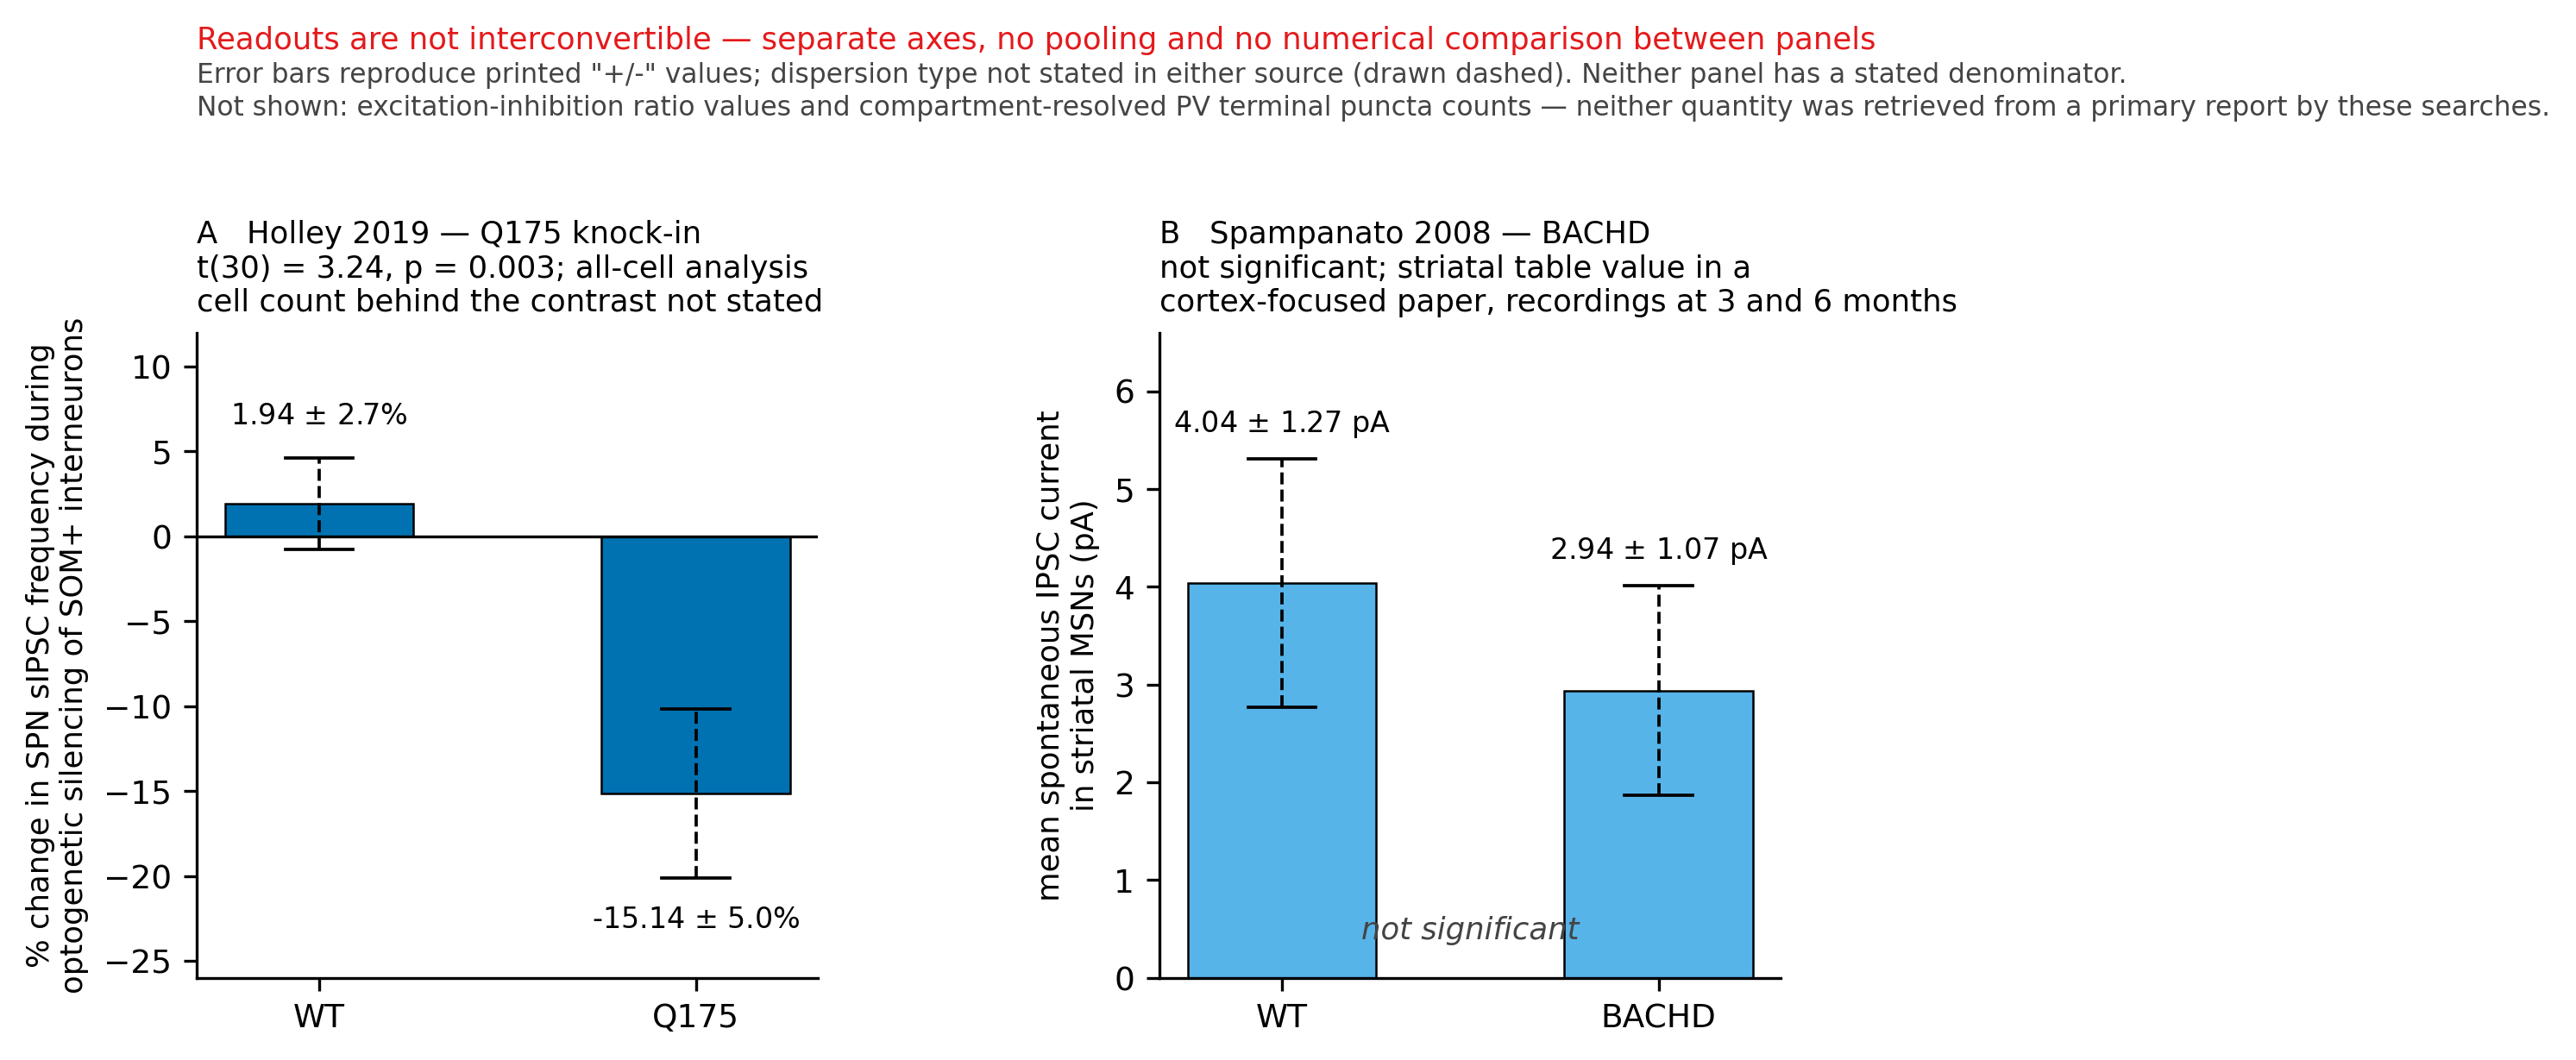
\includegraphics[width=\linewidth]{../figures/fig_sec6_inhibition_onto_projection_neurons_hd.png}
\caption{\textbf{Inhibition received by striatal projection neurons in two Huntington's disease models.} Two single-study genotype contrasts drawn on separate axes and never numerically compared: (A) percent change in spiny projection neuron sIPSC frequency during optogenetic silencing of somatostatin-expressing interneurons, Q175 knock-in versus wild type ($-$15.14 $\pm$ 5.0\% versus 1.94 $\pm$ 2.7\%; t(30) = 3.24, p = 0.003), and (B) mean spontaneous IPSC current in striatal medium spiny neurons, BACHD versus wild type (2.94 $\pm$ 1.07 pA versus 4.04 $\pm$ 1.27 pA, genotype difference not significant). Percent change in sIPSC frequency under interneuron silencing and mean sIPSC current in pA are not interconvertible and are neither pooled nor compared numerically \citep{Holley2019,Spampanato2008}. Silencing in (A) was optogenetic, using enhanced halorhodopsin (eNpHR), not chemogenetic \citep{Holley2019}. The plotted Q175 value is that study's all-cell analysis, whereas the study's own summary attributes the greater decrease to a subset of projection neurons. The number of cells behind the Q175 contrast is not stated in its source, whose test is reported as t(30) = 3.24; no study-wide cell count is quoted because that study's report states none, and the error bars reproduce printed "$\pm$" values whose dispersion type the source does not state. The BACHD mean sIPSC value in (B) is a striatal medium spiny neuron measurement taken from a table in a paper whose reported recordings are cortical, made at 3 and 6 months of age, and the genotype difference is not significant \citep{Spampanato2008}. This figure shows no excitation--inhibition ratio values and no compartment-resolved parvalbumin terminal puncta counts; neither quantity was retrieved from a primary report by these searches.}
\label{fig-sec6-inhibition-onto-projection-neurons-hd}
\end{figure}

\begin{quote}
\noindent\textbf{Evidence Conflict}\par
\textbf{Which interneuron class carries the excess inhibition onto projection neurons.} Silencing somatostatin-expressing interneurons changes projection-neuron sIPSC frequency far more in Q175 than in wild type \citep{Holley2019}; paired recording and optogenetic activation of the same class in R6/2 and knock-in mice find no genotype difference in the responses that class evokes and locate the clearest genotype effect in parvalbumin fast-spiking cells, although the same report notes that somatostatin-expressing cells fire more action potentials in both models and so supply another source of the excess \citep{Cepeda2013}. The two designs differ in what they manipulate (removal of ongoing input versus driven activation), in model and in stage, and the disagreement is unresolved. A parallel disagreement concerns intrinsic physiology: low-threshold-spiking interneuron membrane and synaptic properties are reported unchanged in Q175 at every disease stage, with increased burst firing in a subpopulation of those interneurons in symptomatic mice \citep{Holley2018}, whereas somatostatin interneurons in BACHD mice fire at elevated rates that are normalised by reducing mutant huntingtin in those cells alone \citep{Fowler2026}.

\end{quote}

That second disagreement matters for interpretation, because the BACHD result is the closest thing in this literature to a cell-autonomous test: reducing mutant huntingtin selectively in striatal somatostatin interneurons normalised their firing, implying that the protein acts within cells that do not die \citep{Fowler2026}. The widely repeated claim that interneuron sparing reflects intrinsic, cell-autonomous resistance had no traceable cell-type-restricted genetic experiment behind it in the retrieved literature until tests of this kind, and both this one and its cholinergic counterpart measure physiology rather than survival \citep{Fowler2026,Pancani2023}. Related cell-restricted manipulations point the same way for other classes --- restricting mutant huntingtin to parvalbumin-positive neurons produces hyperactivity with impaired cortical GABA release and blunted gamma-frequency responses without loss of parvalbumin interneurons, a single-study result for which no replication was retrieved in the twelve years since \citep{Dougherty2014}, and presymptomatic bioluminescent-optogenetic manipulation of parvalbumin interneurons, luciferin-driven activation of tethered light-sensing channels, improves motor coordination in R6/2 mice \citep{Ikefuama2025}. Cortical fast-spiking interneuron changes are region-specific within the same model \citep{Wang2023a}. For the somatostatin/NOS class specifically, direct activity measurement in vivo is almost absent: an activity-marker survey of R6/1 striatum detected c-Fos in parvalbumin interneurons but in fewer than 1\% of calretinin-, cholinergic- and nNOS-expressing interneurons, too few for any further analysis \citep{Cabanas2017}. No physiological recording of identified somatostatin interneurons from human HD tissue was retrieved by these searches, so every statement about their activity in HD rests on mouse models that disagree with one another.

The cholinergic interneuron, the other classically spared striatal class, supplies the cleanest demonstration that survival and function are separable. Cholinergic cells in Q140 knock-in mice have simplified dendritic arbors, with significantly fewer and shorter dendrites \citep{Deng2016}; the same class shows enlarged persistent sodium currents \citep{Tanimura2016}, and in zQ175 mice larger evoked inhibitory currents from indirect-pathway collaterals \citep{Lim2021}; in R6/2 mice the same class shows relative resistance to loss, with reductions detectable only at later stages \citep{CrevierSorbo2020}. Lowering mutant huntingtin in those cells alone, but not in cortex or indirect-pathway projection neurons, normalises corticostriatal transmission \citep{Pancani2023}. A surviving population can therefore be the locus of a circuit defect; the consequences for basal ganglia output, including pallidal hyperactivity and excessive inhibition of pallidal targets in early HD \citep{Callahan2022}, are developed in \ref{sec-circuit-consequences}.

\subsection{Aggregates, somatic expansion and the failure of burden to predict death}
\label{sec-06-aggregates-expansion}

Molecular burden does not predict which cells die, and the clearest evidence is quantitative. In early-grade human HD, multiple perikaryal huntingtin aggregates are present in almost all cortical NADPH-diaphorase neurons and in approximately 50\% of the spared striatal NADPH-diaphorase neurons, while the vulnerable spiny neurons carry comparatively few \citep{Kuemmerle1999}; a subset of cortical GABAergic interneurons accumulates aggregates in a striatal-targeted model whose Cre driver is also active in cortical interneuron precursors, an incidental observation rather than a dedicated interneuron-targeted experiment \citep{Gu2007}. Somatic CAG expansion fares no better as a predictor, and on this point the evidence is openly divided. Drd2-expressing striatopallidal indirect-pathway projection neurons are reported to be the more vulnerable of the two projection-neuron subtypes in HD patients \citep{Lee2020}, yet cell-type-resolved measurement in human HD striatum finds no significant difference in somatic repeat expansion between direct- and indirect-pathway neurons, a single-cohort result for which no independent replication was retrieved \citep{Matlik2024}. Whether cell-type-specific somatic expansion explains differential projection-neuron vulnerability is therefore unresolved: one account records the vulnerability gradient \citep{Lee2020} and the other removes its most obvious molecular explanation \citep{Matlik2024}. Spatial transcriptomics of human HD cortex reports that chandelier and somatostatin-positive interneurons are lost despite only modest repeat expansion or aggregation, while within the same preprint the deep-layer excitatory neurons carrying very large somatic expansions are the population reported to undergo severe loss \citep{VazquezSanchez2025}. \ref{fig-sec6-aggregate-burden-versus-cell-death} lays burden and death on a common cell-class axis; the population with abundant aggregates is the one the literature calls spared.

\begin{figure}[H]
\centering
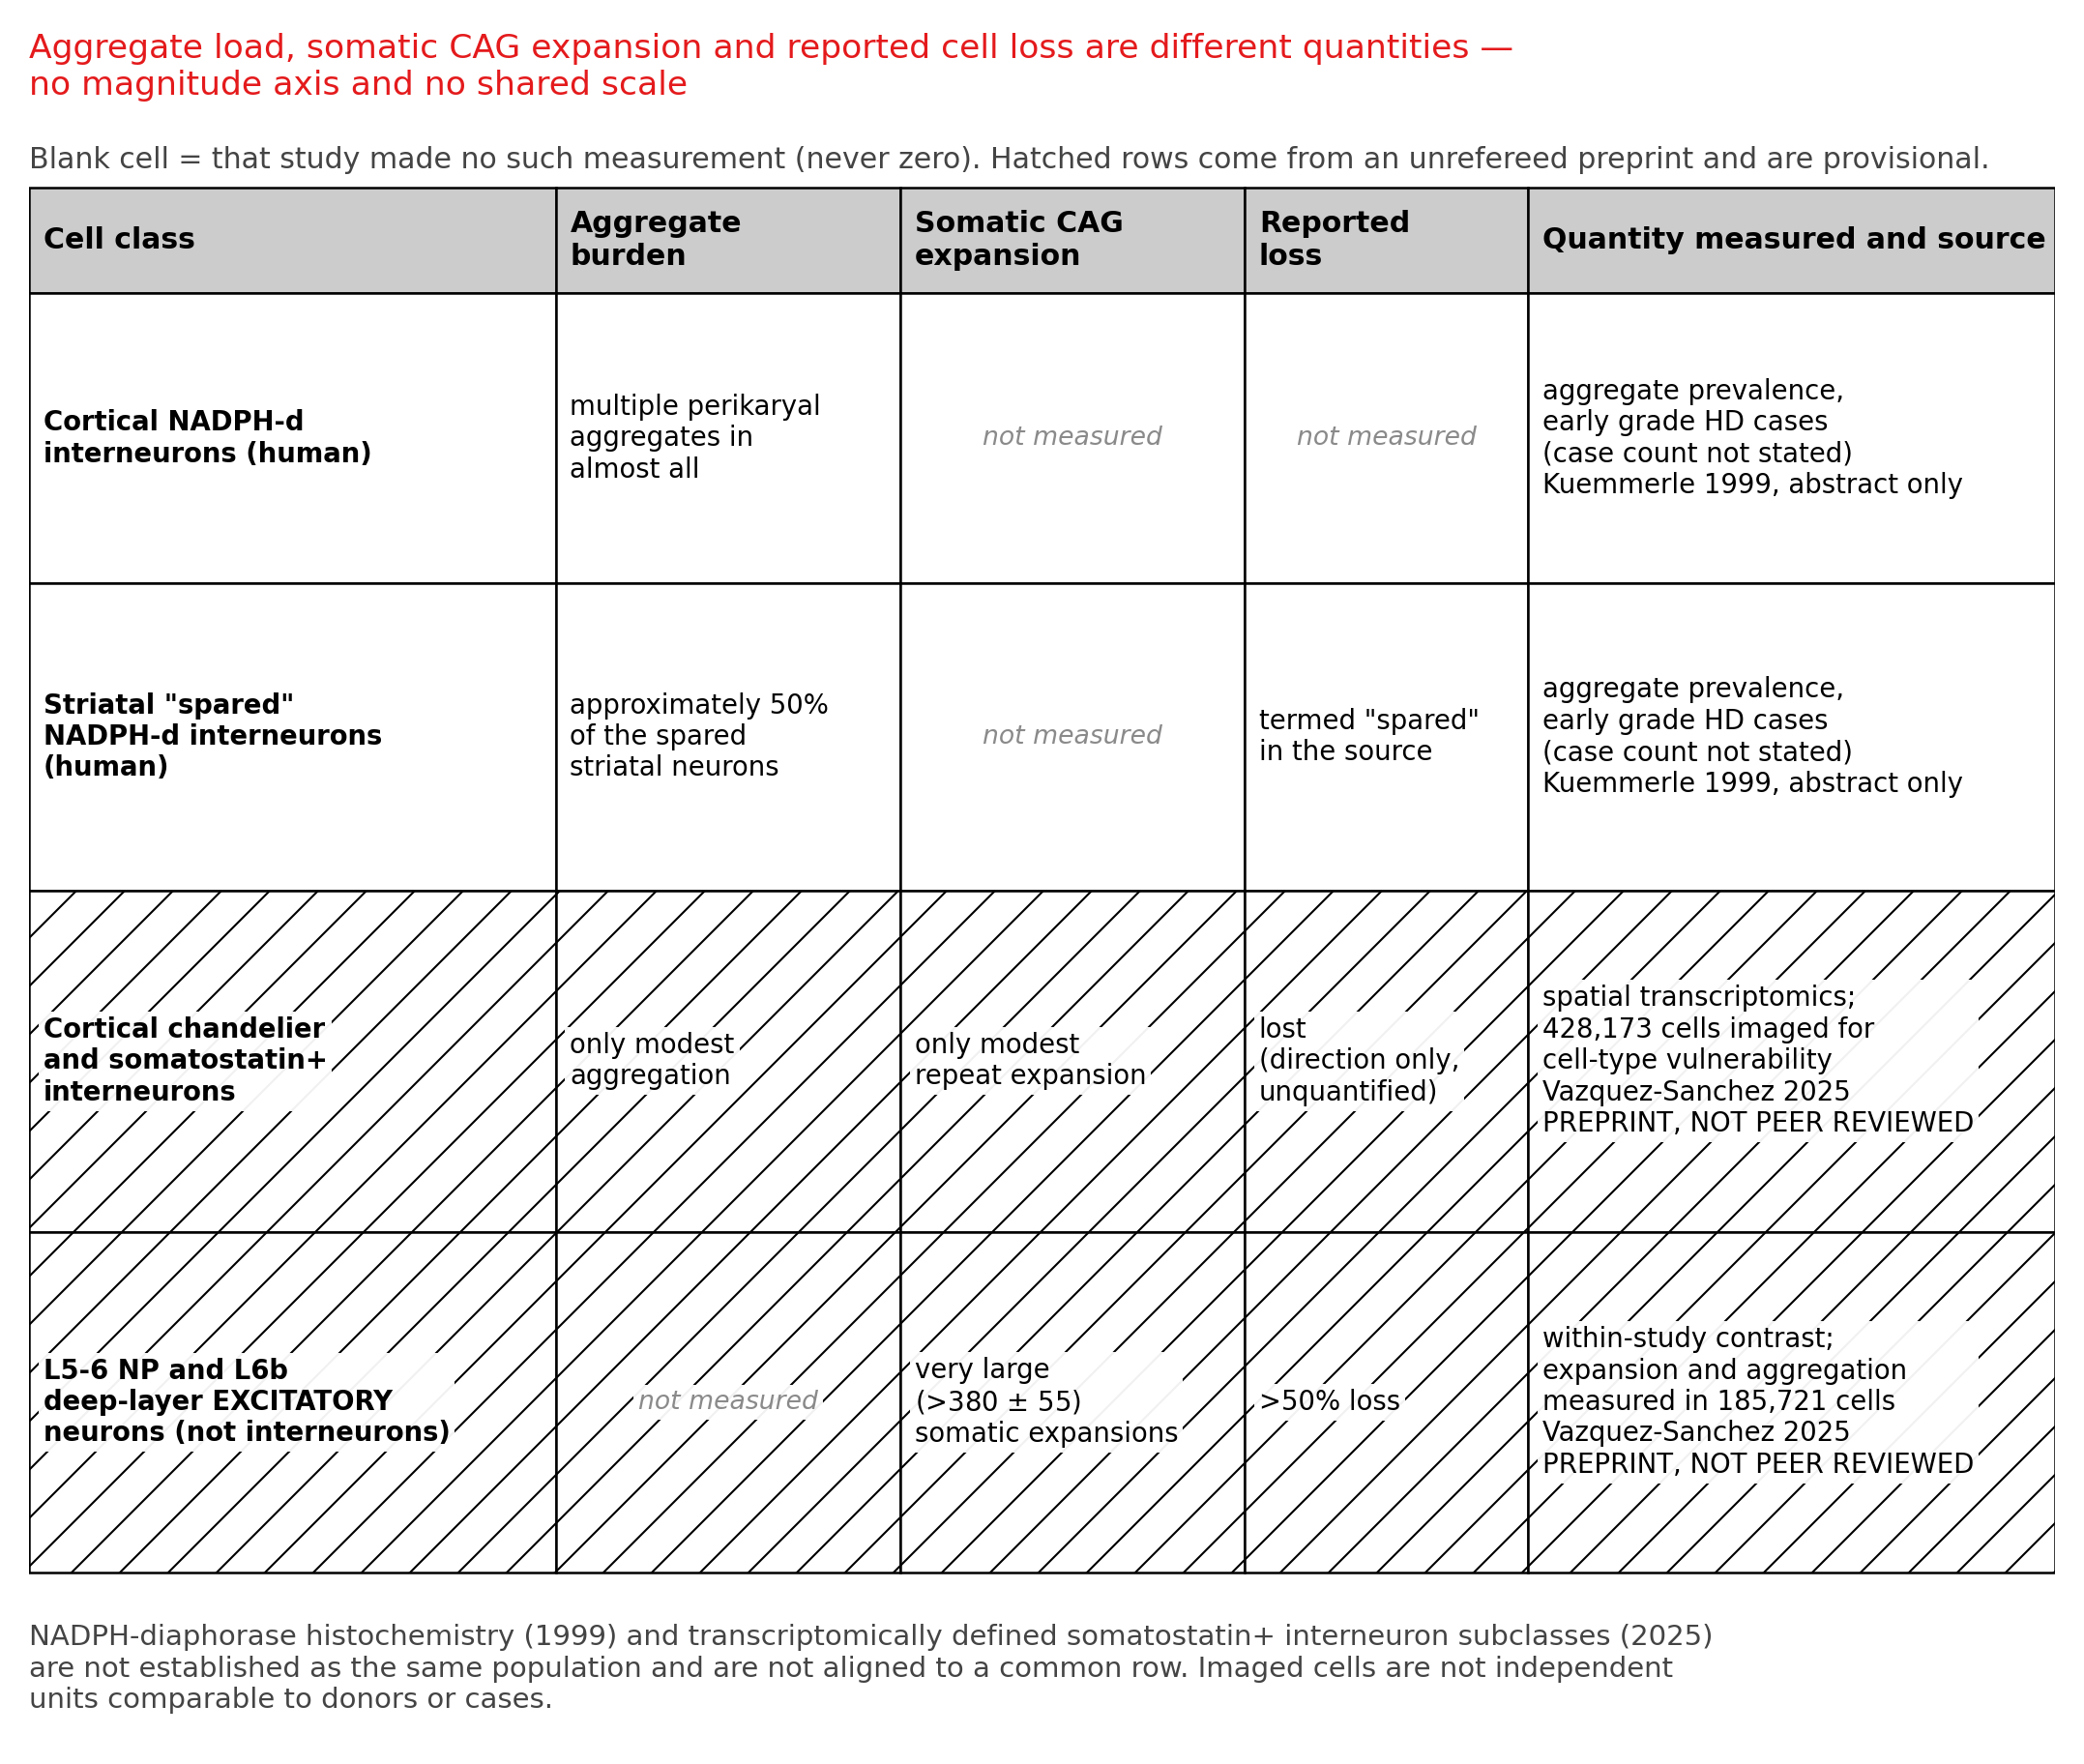
\includegraphics[width=\linewidth]{../figures/fig_sec6_aggregate_burden_versus_cell_death.png}
\caption{\textbf{Aggregate burden, somatic CAG expansion and reported cell loss by cell class.} A qualitative table with no magnitude axis and no bars: aggregate prevalence, somatic CAG repeat expansion and cell loss are distinct quantities, each row reports its own quantity with its own unit, and blank cells mean "not measured", not zero. Within the aggregate-prevalence study the cortical and striatal values differ substantially --- multiple perikaryal aggregates in almost all cortical NADPH-diaphorase neurons versus approximately 50\% of the spared striatal NADPH-diaphorase neurons from early grade cases --- and that regional dissociation is the finding and is not collapsed; the number of HD cases behind it is not stated in the available source \citep{Kuemmerle1999}. Somatostatin-positive and chandelier interneuron loss is reported qualitatively in an unrefereed preprint, so that row is direction-only and provisional, and its provisional status is legible in the table body itself through hatching and an explicit "preprint, not peer reviewed" label rather than only in this caption; the >50\% loss figure belongs to the deep-layer excitatory neuron row alone, which is shown as the within-study contrast to the interneuron row, not as an interneuron measurement \citep{VazquezSanchez2025}. In that study repeat expansion and aggregation were measured in 185,721 cells while the 428,173-cell figure refers to the separate cell-type vulnerability dataset, and cells are not independent units comparable to donors or cases. NADPH-diaphorase histochemistry and transcriptomically defined somatostatin-positive interneuron subclasses are not established as the same population and are not aligned to a common row. This figure shows no direct- versus indirect-pathway projection-neuron repeat-expansion result: the available comparison is a non-significant contrast between projection-neuron subtypes and contains no interneuron measurement \citep{Matlik2024}.}
\label{fig-sec6-aggregate-burden-versus-cell-death}
\end{figure}

What tracks with vulnerability, in the models that have been tested, is projection-neuron identity itself, though the readouts differ widely, from frank degeneration \citep{Noel2018,Oh2022} to spine, calcium and excitability phenotypes \citep{Schmidt2020,Fjodorova2023,Goodliffe2018}. Direct-pathway D1 neurons are significantly altered in aged Q175 heterozygotes while D2 neurons are comparatively less affected, a gradient opposite to the indirect-pathway vulnerability reported in patients \citep{Goodliffe2018,Lee2020}; active caspase-6 degenerates cortical and hippocampal neurons but not striatal medium spiny neurons \citep{Noel2018}; extrasynaptic GluN2B signalling through DAPK1 destabilises medium spiny neuron spines \citep{Schmidt2020}; reduced BCL11B disturbs calcium homeostasis in human stem-cell-derived medium spiny neurons and cortical neurons alike, with the mitochondrial and PKA-dependent calcium-transient deficits confined to the medium spiny neurons \citep{Fjodorova2023}; reprogrammed patient medium spiny neurons from symptomatic donors die selectively \citep{Oh2022}; and HD striatal organoids deplete lateral-ganglionic-eminence progenitors \citep{Wu2024}. Mutant huntingtin reduces striatal synaptic output cell-autonomously \citep{Paraskevopoulou2021}, while deleting wild-type huntingtin in adult cortex and striatum lowers projection-neuron excitability on its own \citep{Barron2026}.

Measurement constraints shape all of this. Striatal interneurons are a small fraction of striatal neurons \citep{Andre2018} resolved into seven transcriptomic populations \citep{Wegman2023}, so surveys of HD striatum have thin interneuron coverage; the interneuron-resolved single-nuclei data retrieved here come from an ovine model \citep{Jiang2024} and the accompanying single-nucleus survey from mouse striatum \citep{Malaiya2021}, not from human tissue, and no human HD single-nucleus dataset with sufficient interneuron depth to test cell-autonomous transcriptional pathology in this class was retrieved, a gap taken up in \ref{sec-human-evidence}. Human in vitro models are not yet a substitute: stem-cell striatal differentiation yields 4.5\% to 12.4\% calretinin interneurons alongside substantial non-striatal fractions \citep{LeCann2021}, and in vivo astrocyte-to-neuron conversion in mouse, a different route to the same cells, produces mostly projection-neuron-like cells, with 8.4\% parvalbumin-positive and under 5\% somatostatin-, NPY- or calretinin-positive \citep{Wu2020}. Viral tools do reach the class \citep{AlMassadi2025}, which makes the cell-restricted experiments above feasible and their continued scarcity notable.

\subsection{Cortex versus striatum, mouse versus human}
\label{sec-06-cortex-striatum}

The sharpest unresolved split is regional and interspecific. Mouse models lose cortical somatostatin-immunoreactive density: progressively in R6/2 motor and anterior cingulate cortex, with somatic shrinkage of 16\%, 15\% and 13\% in somatostatin-, parvalbumin- and VIP-expressing cells but unchanged genetically labelled numbers \citep{Voelkl2022}, and in BACHD cortex, where somatostatin-positive and parvalbumin-positive interneuron counts are both reduced at postnatal day 13 but only the somatostatin deficit is still present at postnatal day 30, traced to aberrant medial ganglionic eminence neurogenesis rather than to degeneration \citep{Molero2026} --- consistent with the finding that conditional loss of wild-type huntingtin in subpallial lineages produces early somatostatin-positive interneuron deficits \citep{Mehler2019}. Functional correlates follow, with NADPH-diaphorase staining reduced in aged male Q175 motor cortex \citep{PadovanNeto2019} and, in a treatment study whose reported outcomes are behavioural rather than cellular, improved motor behaviour with reduced mortality under chronic low-dose epidermal growth factor in R6/2 mice \citep{Marottoli2019}. The human cortical evidence runs the other way or not at all: the older human literature reports increased somatostatin-like immunoreactivity read as cortical sparing \citep{Beal1988}, the human interneuron counts that do exist in HD cortex cover calbindin, calretinin and parvalbumin and report their loss in the anterior cingulate of mood-dominant cases \citep{Kim2014}, and the only retrieved human report of cortical somatostatin interneuron loss is an unrefereed spatial-transcriptomic preprint whose interneuron claim is qualitative \citep{VazquezSanchez2025}. No human stereological or molecular count of somatostatin interneurons in HD cortex was retrieved by these searches, and a caution applies even to the mouse account: the interneuron gene programme most often invoked for cortical HD pathology is predominantly expressed outside interneurons, with non-interneuron forebrain populations accounting for about 80\% of neocortical PGC-1$\alpha$ mRNA \citep{McMeekin2020}. The cortical somatostatin deficit in HD should therefore be stated as a mouse-model finding with a provisional human counterpart, not as an established human phenotype.

\begin{quote}
\noindent\textbf{Evidence Conflict}\par
\textbf{Which cortical interneuron class is most affected, and in which species.} Human HD anterior cingulate cortex loses 80\% of parvalbumin interneurons in mood-dominant cases with calbindin and calretinin losses alongside \citep{Kim2014}, while R6/2 cortex shows unchanged parvalbumin density with reduced somatostatin and VIP immunoreactivity \citep{Voelkl2022}; the most vulnerable cortical subtype differs between human tissue and the model. Overlaying this, human peptide measurements read cortical somatostatin as increased and spared \citep{Beal1988} while a cell-resolved preprint reads somatostatin-positive interneurons as lost \citep{VazquezSanchez2025}, and the canonical striatal synthesis holds the class to be relatively spared \citep{Morigaki2017}. Measurement modality, region and species all separate these claims, and none of the three pairings has been resolved by a study that measures both quantities in the same material.

\end{quote}

HD therefore makes concrete what the preceding disease sections could only suggest: a population can be numerically preserved and functionally abnormal at the same time, a possibility that one model supports directly \citep{Fowler2026} and another does not \citep{Holley2018}, and the measurement that establishes preservation --- peptide concentration, marker-positive profile count, histochemical staining --- is rarely the measurement that would detect the abnormality. The striatal class discussed here is not the cortical Martinotti population defined in \ref{sec-sst-identity} that dominates the rest of this review, which is part of why its literature has developed in near-isolation. The next disease group presents the opposite evidential problem: a condition in which the cell class is barely measured in human tissue at all, and in which the mechanistic account rests on a single mouse study --- the subject of \ref{sec-als-ftd}.

\section{ALS, Frontotemporal Dementia, and Other Neurodegenerative Conditions}
\label{sec-als-ftd}

Striatal interneurons in Huntington's disease, as \ref{sec-huntingtons} showed, are numerically preserved and functionally abnormal; the measurement problem there is that cell counts and peptide content disagree. In amyotrophic lateral sclerosis (ALS) and frontotemporal lobar degeneration (FTLD) the evidential problem inverts. Cortical inhibition is measured in living patients more directly than in most conditions covered here, and the deficit it reveals is one of the most consistently reproduced findings in this literature \citep{Higashihara2024,VanDenBos2024} --- but the cell class this review is about is barely measured in human tissue at all, and the mechanistic account that gives it a leading role rests on one mouse study \citep{Zhang2016}. What follows separates the physiology, which is strong, from the cellular attribution, which is an inference carried by PV counts and, for SST, by a single mouse study.

\subsection{Cortical disinhibition in ALS: robust at the group level, heterogeneous within cohorts}
\label{sec-07-als-disinhibition}

Short-interval intracortical inhibition (SICI), the paired-pulse transcranial magnetic stimulation (TMS) index of GABA-A-mediated cortical inhibition, is reduced in ALS across cohorts and techniques \citep{Higashihara2024,Geevasinga2015}, including a TMS--electroencephalography paired-pulse analogue rather than the conventional motor-evoked-potential measure \citep{VanDenBos2024}, but the reduction is phenotype-dependent: it is absent in a pyramidal phenotype group \citep{Tankisi2025}, and cohorts that stratify patients separate them into hyperexcitable, normally excitable and cortically inexcitable groups \citep{Pavey2024}. \citet{Higashihara2024} pooled threshold-tracking TMS studies and reported a standardised mean difference of $-$0.99 (95\% CI $-$1.12 to $-$0.87, p < 0.001) with moderate heterogeneity (I$^{2}$ = 40\%) --- a pooled meta-analytic estimate over 25 separate threshold-tracking studies. \citet{Geevasinga2015} supplies the single-cohort anatomy of that effect: mean SICI was 1.2\% in C9orf72 familial ALS and 1.6\% in sporadic ALS against 11.8\% in healthy controls, while asymptomatic C9orf72 expansion carriers sat at 10.2\% and did not differ from controls (P = .20), placing inhibitory failure after symptom onset rather than before it. Paired-pulse TMS combined with electroencephalography reproduces the deficit at the level of evoked cortical potentials and shows it scaling with disease duration (P60, P < 0.01; N100, P < 0.005; r = $-$0.698 for the N100 correlation) \citep{VanDenBos2024}. Two results qualify the picture rather than contradicting it: \citet{Tankisi2025} found SICI reduced at all interstimulus intervals in bulbar-onset patients but normal in a pyramidal phenotype group (n = 12 pyramidal, n = 20 classic), and \citet{McMackin2026} found no ALS-versus-control difference in long-interval intracortical inhibition (LICI), the GABA-B-mediated measure (Hedge's g $\leq$ 0.14, P $\geq$ 0.44), a result recorded here as contested relative to the SICI literature. Cortical disinhibition in ALS is therefore specific to a GABA-A circuit, not detectable in the one group of asymptomatic C9orf72 expansion carriers measured here (n = 11), and phenotype-dependent, as \ref{fig-sec7-cortical-inhibition-across-als-cohorts} lays out with each entry on its own units; the presymptomatic rodent evidence discussed below points the other way.

\begin{quote}
\noindent\textbf{Evidence Conflict}\par
\citet{Higashihara2024} present reduced intracortical inhibition as the most sensitive group-level TMS signature of ALS on the strength of a pooled estimate, an aggregate sensitivity rather than a claim about every individual patient, whereas \citet{Pavey2024} phenotyped 417 patients with the same technique and found cortical hyperexcitability in 210 (50.3\%), frank cortical inexcitability in 110 (26.4\%) and normal excitability in 97 (23.3\%). The disagreement is between a pooled mean effect and a within-cohort distribution, and it bears directly on whether GABAergic interneuron failure is a disease-wide or a subgroup phenomenon. It is partially resolved: a large mean reduction and a bimodal cohort are arithmetically compatible, because the cortically inexcitable quarter contributes no SICI value at all rather than a normal one. What would settle it --- a longitudinal within-patient study tracking transition between excitability phenotypes --- has not been reported in the material retrieved here, and no primary data reconciling the pooled estimate with the distribution were found.

\end{quote}

The same measures in frontotemporal degeneration are pharmacological rather than purely observational, and they are the strongest interventional evidence in this section for a GABAergic contribution to a cortical physiological index in these dementias; the drug effect recorded here is on that index, not a reversal of the behavioural deficit. Magnetic resonance spectroscopy shows reduced GABA in right inferior frontal cortex but not occipital cortex in behavioural-variant frontotemporal dementia (bvFTD) and progressive supranuclear palsy, with the frontal GABA and glutamate deficits tracking failures of response inhibition (F(1) = 8.67, P = 0.005; occipital P = 0.81) \citep{Murley2020}; enhancing GABA with tiagabine normalises task-related beta power in the same region \citep{Hughes2025}; and generative modelling of magnetoencephalography, recorded under an auditory oddball paradigm rather than the response-inhibition task, infers increased tonic inhibition of deep inhibitory populations \citep{Adams2021}. That last inference needs a caveat the source itself implies: the inhibitory "populations" of a dynamic causal model are model parameters, not counted cells, and no interneuron is measured by that method. Reviews that assemble this material around PV interneuron dysfunction as the shared substrate of cortical hyperexcitability across dementias \citep{Smeralda2024} are restating a hypothesis, not a measurement, and the cerebrospinal fluid peptide literature is correspondingly fragile: somatostatin and NPY are correlated with each other in FTD (n = 22) but not in Alzheimer's disease (n = 34) (p < 0.02) \citep{Minthon1997}, and CSF somatostatin in demented patients rises over three months of an activating care programme \citep{WiderloV1989}, which makes it a state-dependent measure rather than a fixed index of interneuron integrity --- a point developed in \ref{sec-human-evidence}.

Rodent work supplies the causal arrow that human recordings cannot. Chemogenetically raising the activity of layer 5 motor-cortex PV interneurons in late pre-symptomatic SOD1-G93A mice restores intracortical inhibition, reduces pyramidal hyperexcitability, delays motor deficit onset and extends survival \citep{Khademullah2020}; inhibitory interneuron pathology precedes motor neuron loss in spinal cord across several models, including depletion of V1 subpopulations at P63 and P112 \citep{MontananaRosell2024}, early glycinergic stress and reduced synaptic output in mutant sod1 zebrafish \citep{McGown2012}, morphological and functional changes in GlyT2+ interneurons \citep{Cavarsan2023}, and failure of depolarising inhibitory events to control low-input-resistance motoneurons embryonically \citep{Zhu2024}. Cortical GABAergic interneurons in the same model remodel structurally while losing intrinsic excitability (neurite path length 3380 $\mu$m against 2363 $\mu$m in wild type) \citep{Clark2018}, and NPY-expressing interneuron density rises by 29\% supragranularly and 30\% infragranularly in motor but not somatosensory cortex \citep{Clark2017} --- remodelling, not simply depletion. Two results bound the generality: progressive dynein impairment causes motor axonal pathology without loss of any major spinal interneuron population \citep{Christoforidou2026}, and TrkB.T1 deletion restores PV interneuron numbers to physiological level in the mutant SOD1 hippocampus, the result that study reports for CA1, while in CA3 the compensation is incomplete (344.79 $\pm$ 27.13 against 433.86 $\pm$ 118.50 in wild type, p < 0.001) \citep{Quarta2018}. The C9orf72 promoter is active in inhibitory as well as excitatory neurons, so a cell-autonomous route is possible \citep{Langseth2017}.

\begin{quote}
\noindent\textbf{Evidence Conflict}\par
\citet{Amalyan2022} report that asymptomatic C9orf72 model mice already show reduced inhibitory drive onto surviving primary motor cortex layer 5 pyramidal neurons, with enhanced cortical output during high-speed locomotion, whereas \citet{Bonthron2024} find no change in the relative abundance of excitatory versus inhibitory synapses onto spinal motor neurons at presymptomatic stages across multiple ALS models. The compartments differ --- functional inhibitory drive onto cortical pyramidal neurons against anatomical synaptic puncta ratios onto spinal motor neurons --- as do the genotypes, so the two are not strictly incompatible; both are recorded as contested. Status: open. The disagreement matters because the widely repeated claim that interneuron loss causes rather than follows cortical hyperexcitability in ALS has no primary demonstration in human tissue: the human evidence retrieved here is either an indirect paired-pulse physiological proxy or a cross-sectional post-mortem density, and the causal experiments exist only in rodents.

\end{quote}

\subsection{Which interneurons? PV depletion is measured, SST is inferred}
\label{sec-07-pv-versus-sst}

Where cells are counted in these conditions, the marker is almost always parvalbumin, and the reported reductions cluster in a band around a quarter to a half. In TDP-43 proteinopathy, \citet{Lin2021} found PV+ interneuron density reduced by 27.1\% in mouse frontal cortex, by 50.1\% in cingulate cortex, and by 24.6\% in post-mortem human ALS cortex including C9orf72-linked and sporadic cases; \citet{White2018} reported a \textasciitilde{}25\% reduction in frontal cortex of the same TDP-43 Q331K knock-in line, which makes it a confirmation within one model rather than an independent replication, and \citet{Lin2020} traced the deficit back to postnatal day 14 while reporting the same paucity in human sporadic and C9orf72 ALS prefrontal cortex. Comparable magnitudes recur under unrelated insults: 47.6\% and 31.5\% reductions in PVALB+ cell density in the motor cortex of post-mortem progressive multiple sclerosis (MS) cases stratified by meningeal inflammation \citep{Magliozzi2021}, layer-selective interneuron loss beneath subpial MS lesions \citep{Nicholas2015}, selective layer 2 PV loss with calretinin cells unchanged in MS motor cortex \citep{Clements2008}, a 52.2\% reduction in PV-occupied cortical area in experimental autoimmune encephalomyelitis \citep{Falco2014}, 29.53\% and 45.73\% reductions in layer 5 PV density at seven days and one month after blast injury in a rat model \citep{May2024}, 39\% in the dentate gyrus after status epilepticus \citep{Mishra2015}, and a 42\% total reduction over the study interval in wobbler mouse hippocampus against 18\% in controls \citep{Thielsen2013}. \ref{fig-sec7-pv-versus-sst-depletion-across-conditions} puts these side by side without pooling them, because the convergence is partly an artefact of a shared metric: an area fraction, a stereological count and an uncorrected within-group reduction are not one quantity.

\begin{quote}
\noindent\textbf{Evidence Conflict}\par
Against that convergence, \citet{MerinoSerrais2025} quantified PV+ neuron density in human post-mortem hippocampal formation and entorhinal cortex with phospho-tau staging and reported the two groups as similar (11.2 $\pm$ 15.3 neurons/mm$^{2}$ in non-demented against 9.7 $\pm$ 15.8 in dementia cases), with no statistical test reported for that comparison and the region behind the two densities --- hippocampal formation, entorhinal cortex or both --- not resolved in the available material; the standard deviation exceeds the mean in both groups. Region, species and proteinopathy all differ from \citet{Lin2021} --- frontal cortex in a TDP-43 knock-in mouse plus ALS cortex, against human hippocampal formation in tau-associated dementia --- so the conflict is as much about where one counts as about whether PV cells die. Status: open, and this study is itself recorded as contested. The deeper problem is that nearly every deficit above is immunoreactivity-based: no study combining a PV-independent interneuron label with PV immunoreactivity in the same degenerating human tissue was retrieved by these searches, so marker downregulation and cell death remain unseparated, and the therapeutic implication inverts between them.

\end{quote}

The SST evidence in these conditions is thinner and partly measures something else. The quantitative entries are a 46\% reduction in SST+ interneurons in the dentate gyrus after status epilepticus --- larger than the 39\% PV reduction in the same study and smaller than the 56\% NPY reduction \citep{Mishra2015} --- a \textasciitilde{}65\% loss of virally labelled hilar SST cells after traumatic brain injury (TBI), with rabies-traced starter neurons collapsing from 48.0 $\pm$ 3.7 to 9.4 $\pm$ 0.9 \citep{Frankowski2022}, a \textasciitilde{}20\% decrease reported jointly for PV and SST interneurons in CA1 of aged tau transgenic mice \citep{Levenga2013}, and, in a tau/amyloid rat, dystrophic tau-bearing SST neurons making up more than 40\% of the hippocampal SST population at 15 months while PV neurons are relatively preserved \citep{Morrone2022} --- the tau-bearing dystrophic survivors described in \ref{sec-alzheimers}. The last of those is a pathology burden, not a loss. Transcript-level work reaches the population without counting cells, though mostly outside human ALS tissue: somatostatin, NPY and cholecystokinin transcripts are downregulated in the brainstem of cattle with bovine spastic paresis \citep{Krull2025}, GABAergic neurons rank as the most transcriptionally perturbed neuronal population in mutant SOD1 brainstem (1.77\% of expressed genes differentially expressed), a single-cohort ranking not independently reproduced in the retrieved record \citep{Liu2020a}, TDP-43 loss of function in medial prefrontal cortex identifies GABAergic neurons as selectively vulnerable \citep{Thapa2025}, TDP-43 overexpression accelerates age-dependent interneuron degeneration with interneuron-derived ubiquitin aggregates \citep{Tsuiji2017}, and a single-nucleus atlas of human antero-median thalamus in GRN-associated and sporadic TDP-43 FTD (331,065 nuclei from 92 individuals, a preprint) finds two inhibitory populations markedly depleted \citep{Trujillo2026}. What does not exist in the retrieved record is the obvious measurement: no direct quantification of SST interneuron density, morphology or transcriptional state in post-mortem human ALS or FTLD cortex was retrieved by these searches, and the human cortical quantifications in this literature measure parvalbumin. The contrast with the Alzheimer single-nucleus cohorts of \ref{sec-human-evidence} is stark.

\begin{quote}
\noindent\textbf{Evidence Conflict}\par
Whether reduced SST-immunoreactive counts after an insult mean interneuron death is directly contested. \citet{Buckmaster1999} read the missing cells as selective death, reporting that interneuron loss in the epileptic hippocampus is remarkably specific, with 83\% of the missing GAD-positive neurons somatostatin-immunoreactive; \citet{Drake2024} fate-mapped the same population genetically in a Pten knockout epilepsy model and found density reduced by roughly 13--22\% across subregions (hilar 4,395 $\pm$ 182 against 3,411 $\pm$ 322 cells/mm$^{3}$, p = 0.0334) with no increase in oxidative-stress or apoptosis markers (3-nitrotyrosine-positive proportion 38.47\% against 38.61\%, p = 0.9684), retained SST phenotype among labelled cells (84.17\% against 84.76\%, p = 0.8212) and preserved axonal output density. The dimension of disagreement is what was counted --- antibody-defined somata against genetically labelled cells with phenotype and output measured in parallel. Status: unresolved --- the two studies examine different epileptogenic models, and no experiment applying both readouts to the same tissue was retrieved by these searches. The direction-of-change literature is unstable for the same reason: chronic pilocarpine epilepsy shows fewer SST- and NPY-immunoreactive hilar interneurons \citep{Long2010}, whereas kindling and electrically induced status epilepticus show markedly increased SST and NPY immunoreactivity and mRNA in the same population \citep{Vezzani1996} --- partially resolved as a difference of timepoint and insult severity, which is precisely the condition under which peptide immunoreactivity fails as a surrogate for interneuron survival.

\end{quote}

\subsection{The SST-driven disinhibition model and its single source}
\label{sec-07-tdp43-model}

The mechanistic account that gives SST interneurons a leading role in ALS/FTD comes from one paper. \citet{Zhang2016} recorded from a TDP-43 transgenic mouse motor cortex crossed to Sst-Cre and Pv-Cre reporter lines and found SST interneurons hyperactive --- with significantly increased spontaneous but normal miniature inhibitory postsynaptic currents at three weeks, persisting into adulthood --- while PV interneurons were hypoactive, and argued that SST-driven suppression of PV cells disinhibits layer 5 pyramidal neurons and contributes to excitotoxicity. The recordings are from more than ten neurons in at least three mice per group; the circuit logic depends on the SST$\rightarrow$PV connection described in \ref{sec-sst-identity}. This is the clearest case in this review of an influential mechanism carried by a single study: it is recorded as replication-unknown ten years after publication, and no independent laboratory reproduction was retrieved. The alternative account in the wobbler mouse runs in the opposite direction, which is the section's mechanistic fork.

\begin{quote}
\noindent\textbf{Evidence Conflict}\par
\citet{Zhang2016} attribute layer 5 pyramidal hyperexcitability in TDP-43 mice to hyperactive SST interneurons suppressing PV cells, whereas \citet{NietoGonzalez2010} attribute motor cortex hyperexcitability in the wobbler mouse to globally reduced GABAergic inhibition --- the frequency of GABA-A-mediated spontaneous inhibitory postsynaptic currents in layer 5 pyramidal neurons was reduced by 72\% --- alongside decreased numbers of both PV- and SST-immunoreactive interneurons. The dimension of disagreement is whether SST interneurons are functionally gained or numerically lost, and whether disinhibition is a circuit-specific SST-to-PV effect or the consequence of overall interneuron depletion. Status: open. The models differ in construct and in what was counted, and the wobbler result is available here only at abstract level, so the comparison is between a cell-type-resolved optogenetic/electrophysiological dissection in one transgenic line and a mixed physiological and immunohistochemical account in another.

\end{quote}

\begin{figure}[H]
\centering
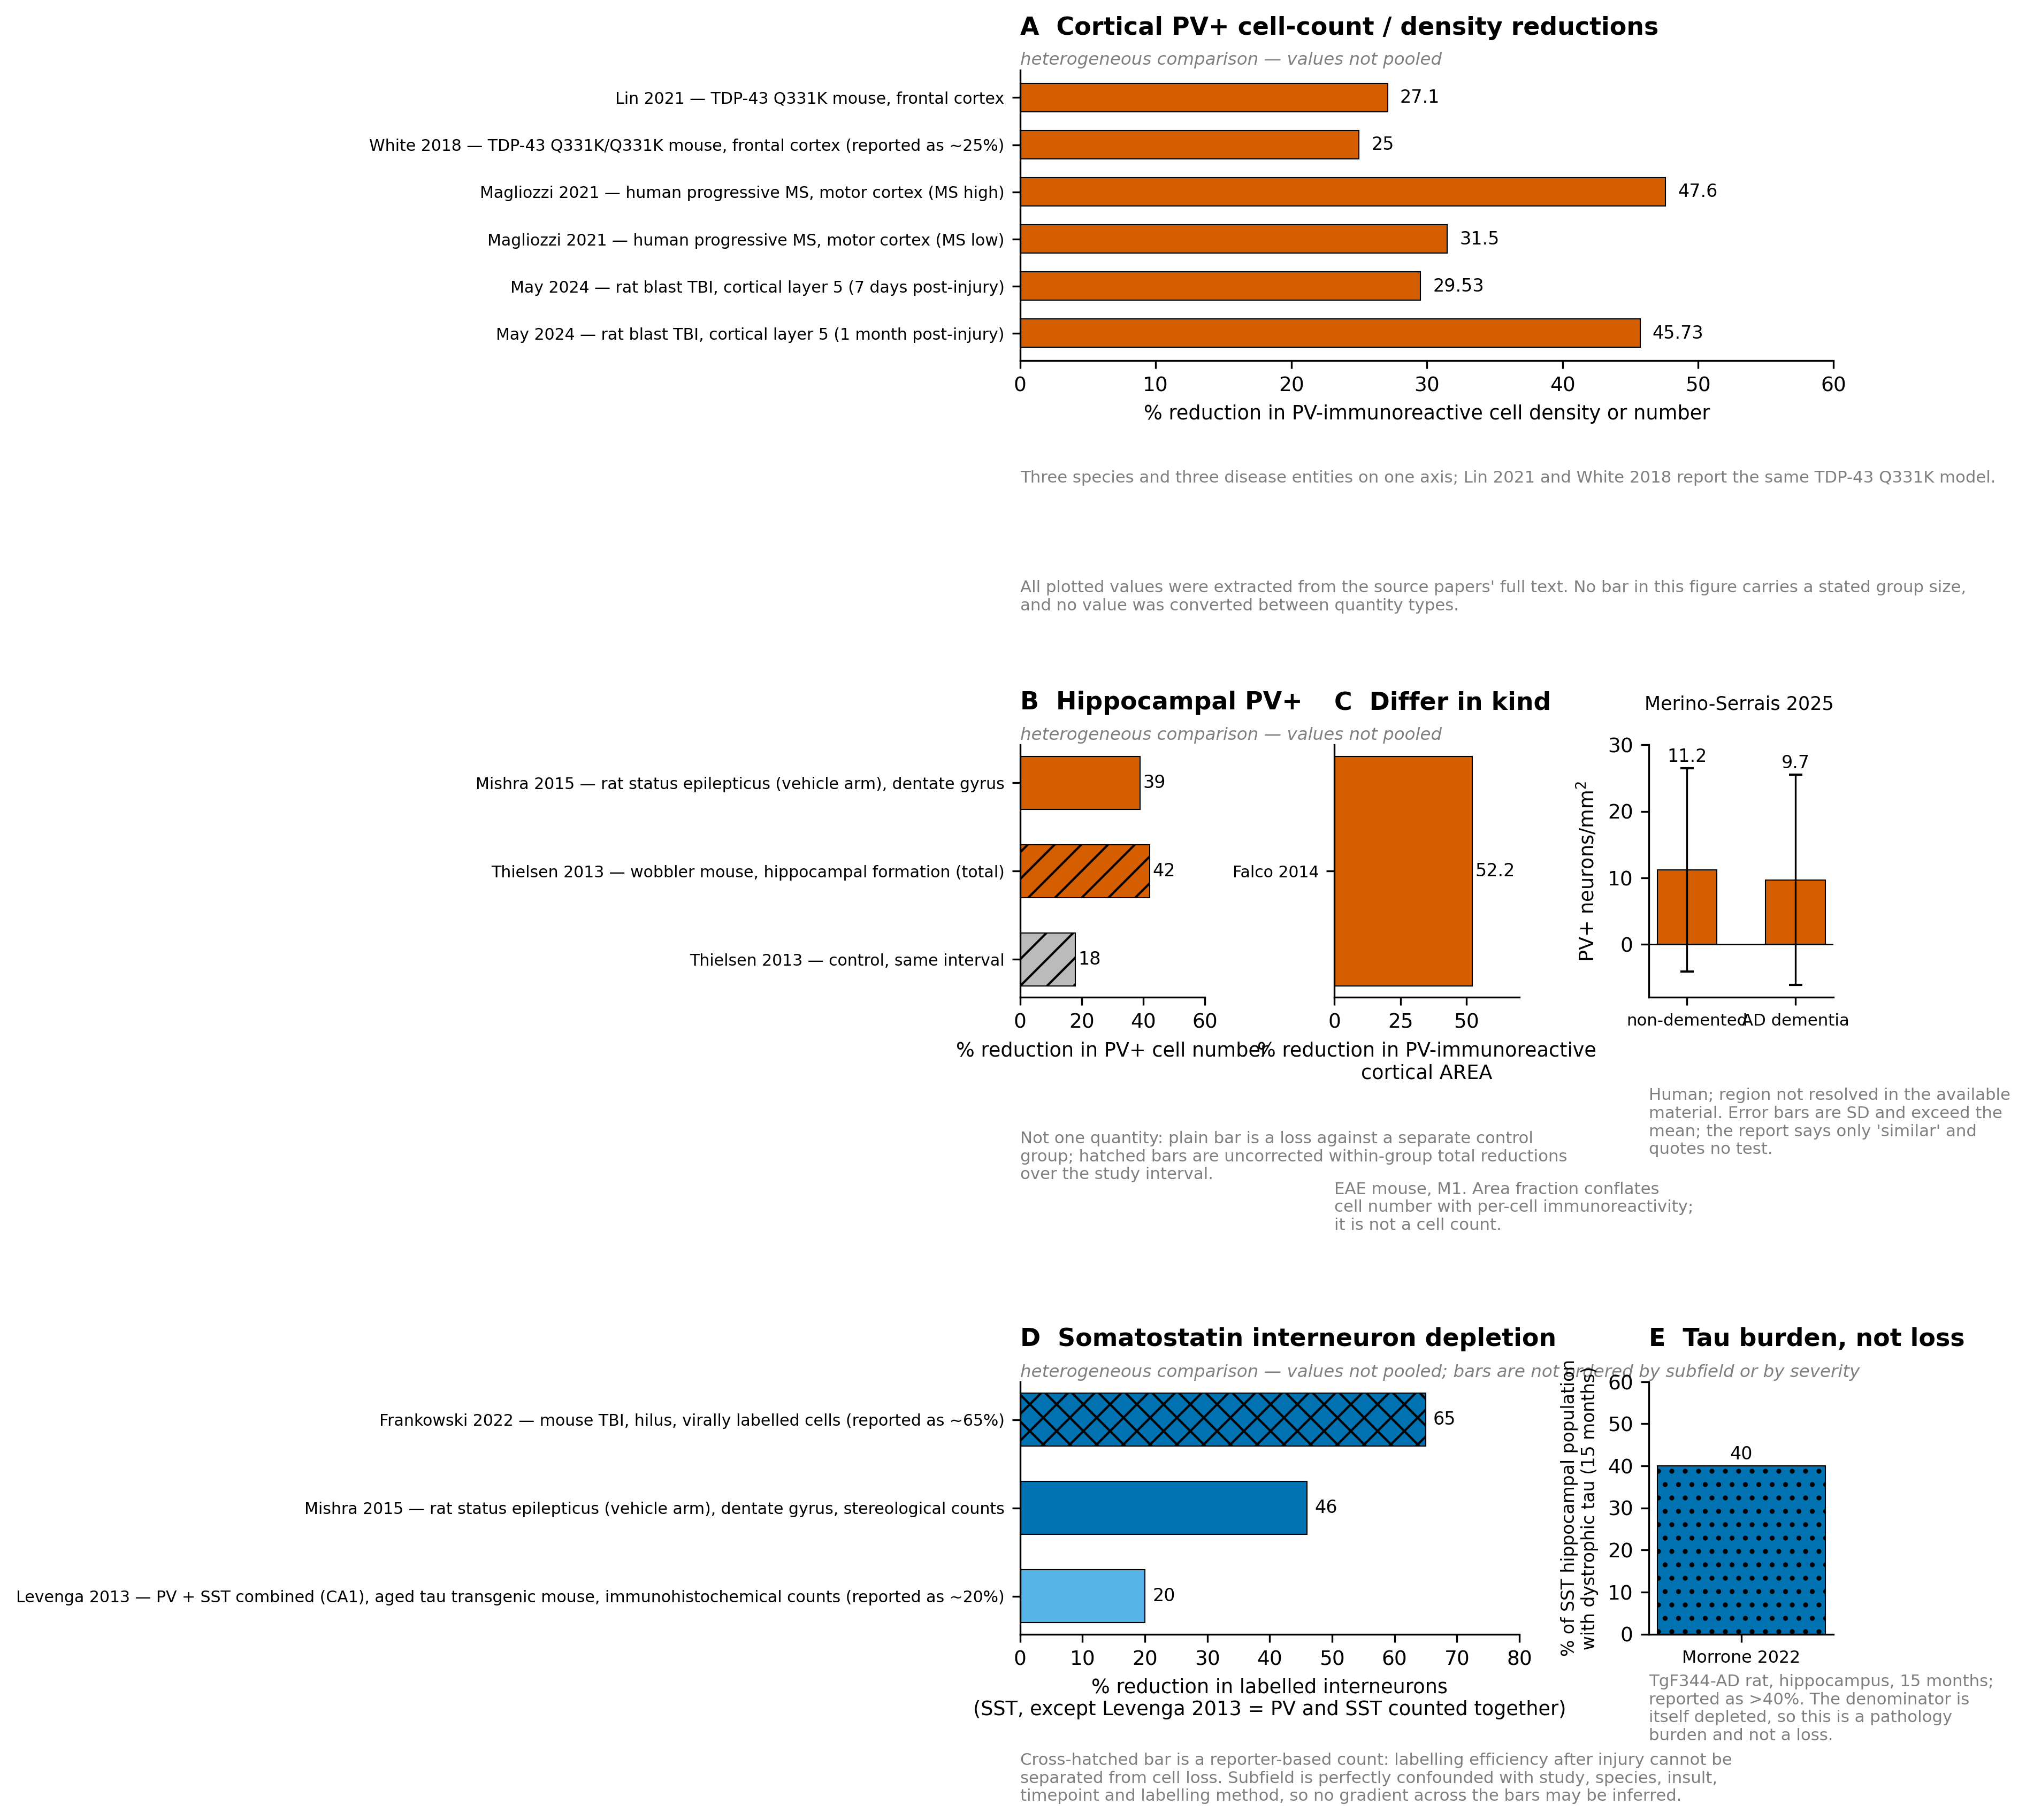
\includegraphics[width=\linewidth]{../figures/fig_sec7_pv_versus_sst_depletion_across_conditions.png}
\caption{\textbf{Parvalbumin and somatostatin depletion across neurodegenerative and injury conditions, grouped by measured quantity.} Panels group entries by what was measured and where: panel A cortical PV+ cell-count/density reductions, panel B hippocampal PV+ cell-count reductions, panel C the two PV entries whose quantity differs in kind, panel D SST depletion, panel E a tau-pathology burden. No value was converted between quantity types and nothing is pooled. Values are not a single measurement type: bars for Lin 2021, White 2018, Magliozzi 2021, May 2024 and Mishra 2015 are percentage reductions in PV+ cell density or number; Falco 2014 is the percentage reduction in PV-immunoreactive cortical AREA, which conflates cell number with per-cell immunoreactivity; Merino-Serrais 2025 is an absolute density in neurons/mm$^{2}$. Panel A pools three species and three disease entities on one axis --- TDP-43 Q331K knock-in mouse (ALS-FTD), human post-mortem progressive multiple sclerosis, and rat mild blast traumatic brain injury --- and bar heights are not comparable across these systems. May 2024 is a rat model of mild blast traumatic brain injury. Panel B's axis is not one quantity: Mishra 2015's 39\% is a loss relative to a separate control group, whereas Thielsen 2013's 42\% and the 18\% control bar are uncorrected within-group total reductions over the study interval, so the 42\% must not be read as disease-attributable loss; Thielsen 2013's PV+ counts are reported for all areas of the hippocampal formation except the hilus, and the value plotted here is that study's total reduction rather than any single subfield. Regions are not matched: frontal cortex (Lin 2021's plotted value is the mouse frontal cortex, not the human post-mortem arm), motor cortex, cortical layer 5, dentate gyrus and hippocampus are each represented; Mishra 2015's loss is reported for the dentate gyrus, not the whole hippocampus, and Falco 2014's M1 cell-number reduction is reported for layers II and III. Lin 2021 and White 2018 report the same TDP-43 Q331K knock-in model and must not be read as independent replication. Magliozzi 2021's abstract reports 40 post-mortem progressive MS cases (with/without meningeal inflammation) and 10 control cases; whether that cohort is the same as the second, independent post-mortem group supplying the plotted 47.6\% and 31.5\% cannot be determined from the material available, and no MS-high / MS-low group size is stated anywhere. No bar in this figure carries a group size, and dispersion is plotted only for Merino-Serrais 2025, whose standard deviation exceeds its mean in both groups, so apparent rank order between bars is not statistically supported. The abstract of Magliozzi 2021 additionally reports a different figure (51.8) for PVALB+ cell density in cortical lesions in patients with high meningeal inflammation, which is not plotted. Mishra 2015's values are the vehicle (untreated) arm of a resveratrol intervention study. Merino-Serrais 2025's report describes the two densities as similar and quotes no statistical test, so the entry is not labelled "no significant difference"; the sentence reporting them names no region, and because that study's analysis covers the hippocampal formation and the entorhinal cortex the two bars are labelled "region not resolved in the available material". Panel D's axis carries the population qualifier because the quantity is not uniformly SST-specific: Levenga 2013's \textasciitilde{}20\% is reported jointly for PV and SST interneurons in CA1 and is labelled in-panel as such. Frankowski 2022's \textasciitilde{}65\% is the loss of Cre-dependent virally labelled (GFP+) hilar cells, and reduced labelling efficiency after injury cannot be separated from cell loss. Morrone 2022's value is the fraction of the SST hippocampal population at 15 months bearing dystrophic tau pathology, not SST cell loss, and sits on its own panel E axis; its denominator is itself depleted, since that study's abstract states that by 15 months the TgF344-AD rats had robust loss of excitatory and inhibitory neurons. In panel D, subfield is perfectly confounded with study, species, insult, timepoint and labelling method --- one study per subfield (dentate gyrus, Mishra 2015; hilus, Frankowski 2022; CA1, Levenga 2013; hippocampus, Morrone 2022) --- so no part of the spread can be attributed to subfield and no gradient across the bars may be inferred; the bars are therefore not ordered by subfield or by severity, and each carries its species, insult, region and counting method on its in-panel label. The injury descriptors that identify each model more precisely appear only in the papers' article text, not in the abstracts available for this figure, and are therefore not shown on the bars. No entry in panel D or E carries a stated group size, so no bar is better powered than another and no rank order between bars is statistically supported. Sources: \citep{Lin2021,White2018,Magliozzi2021,May2024,Mishra2015,Thielsen2013,Falco2014,MerinoSerrais2025,Frankowski2022,Levenga2013,Morrone2022}.}
\label{fig-sec7-pv-versus-sst-depletion-across-conditions}
\end{figure}

\begin{figure}[H]
\centering
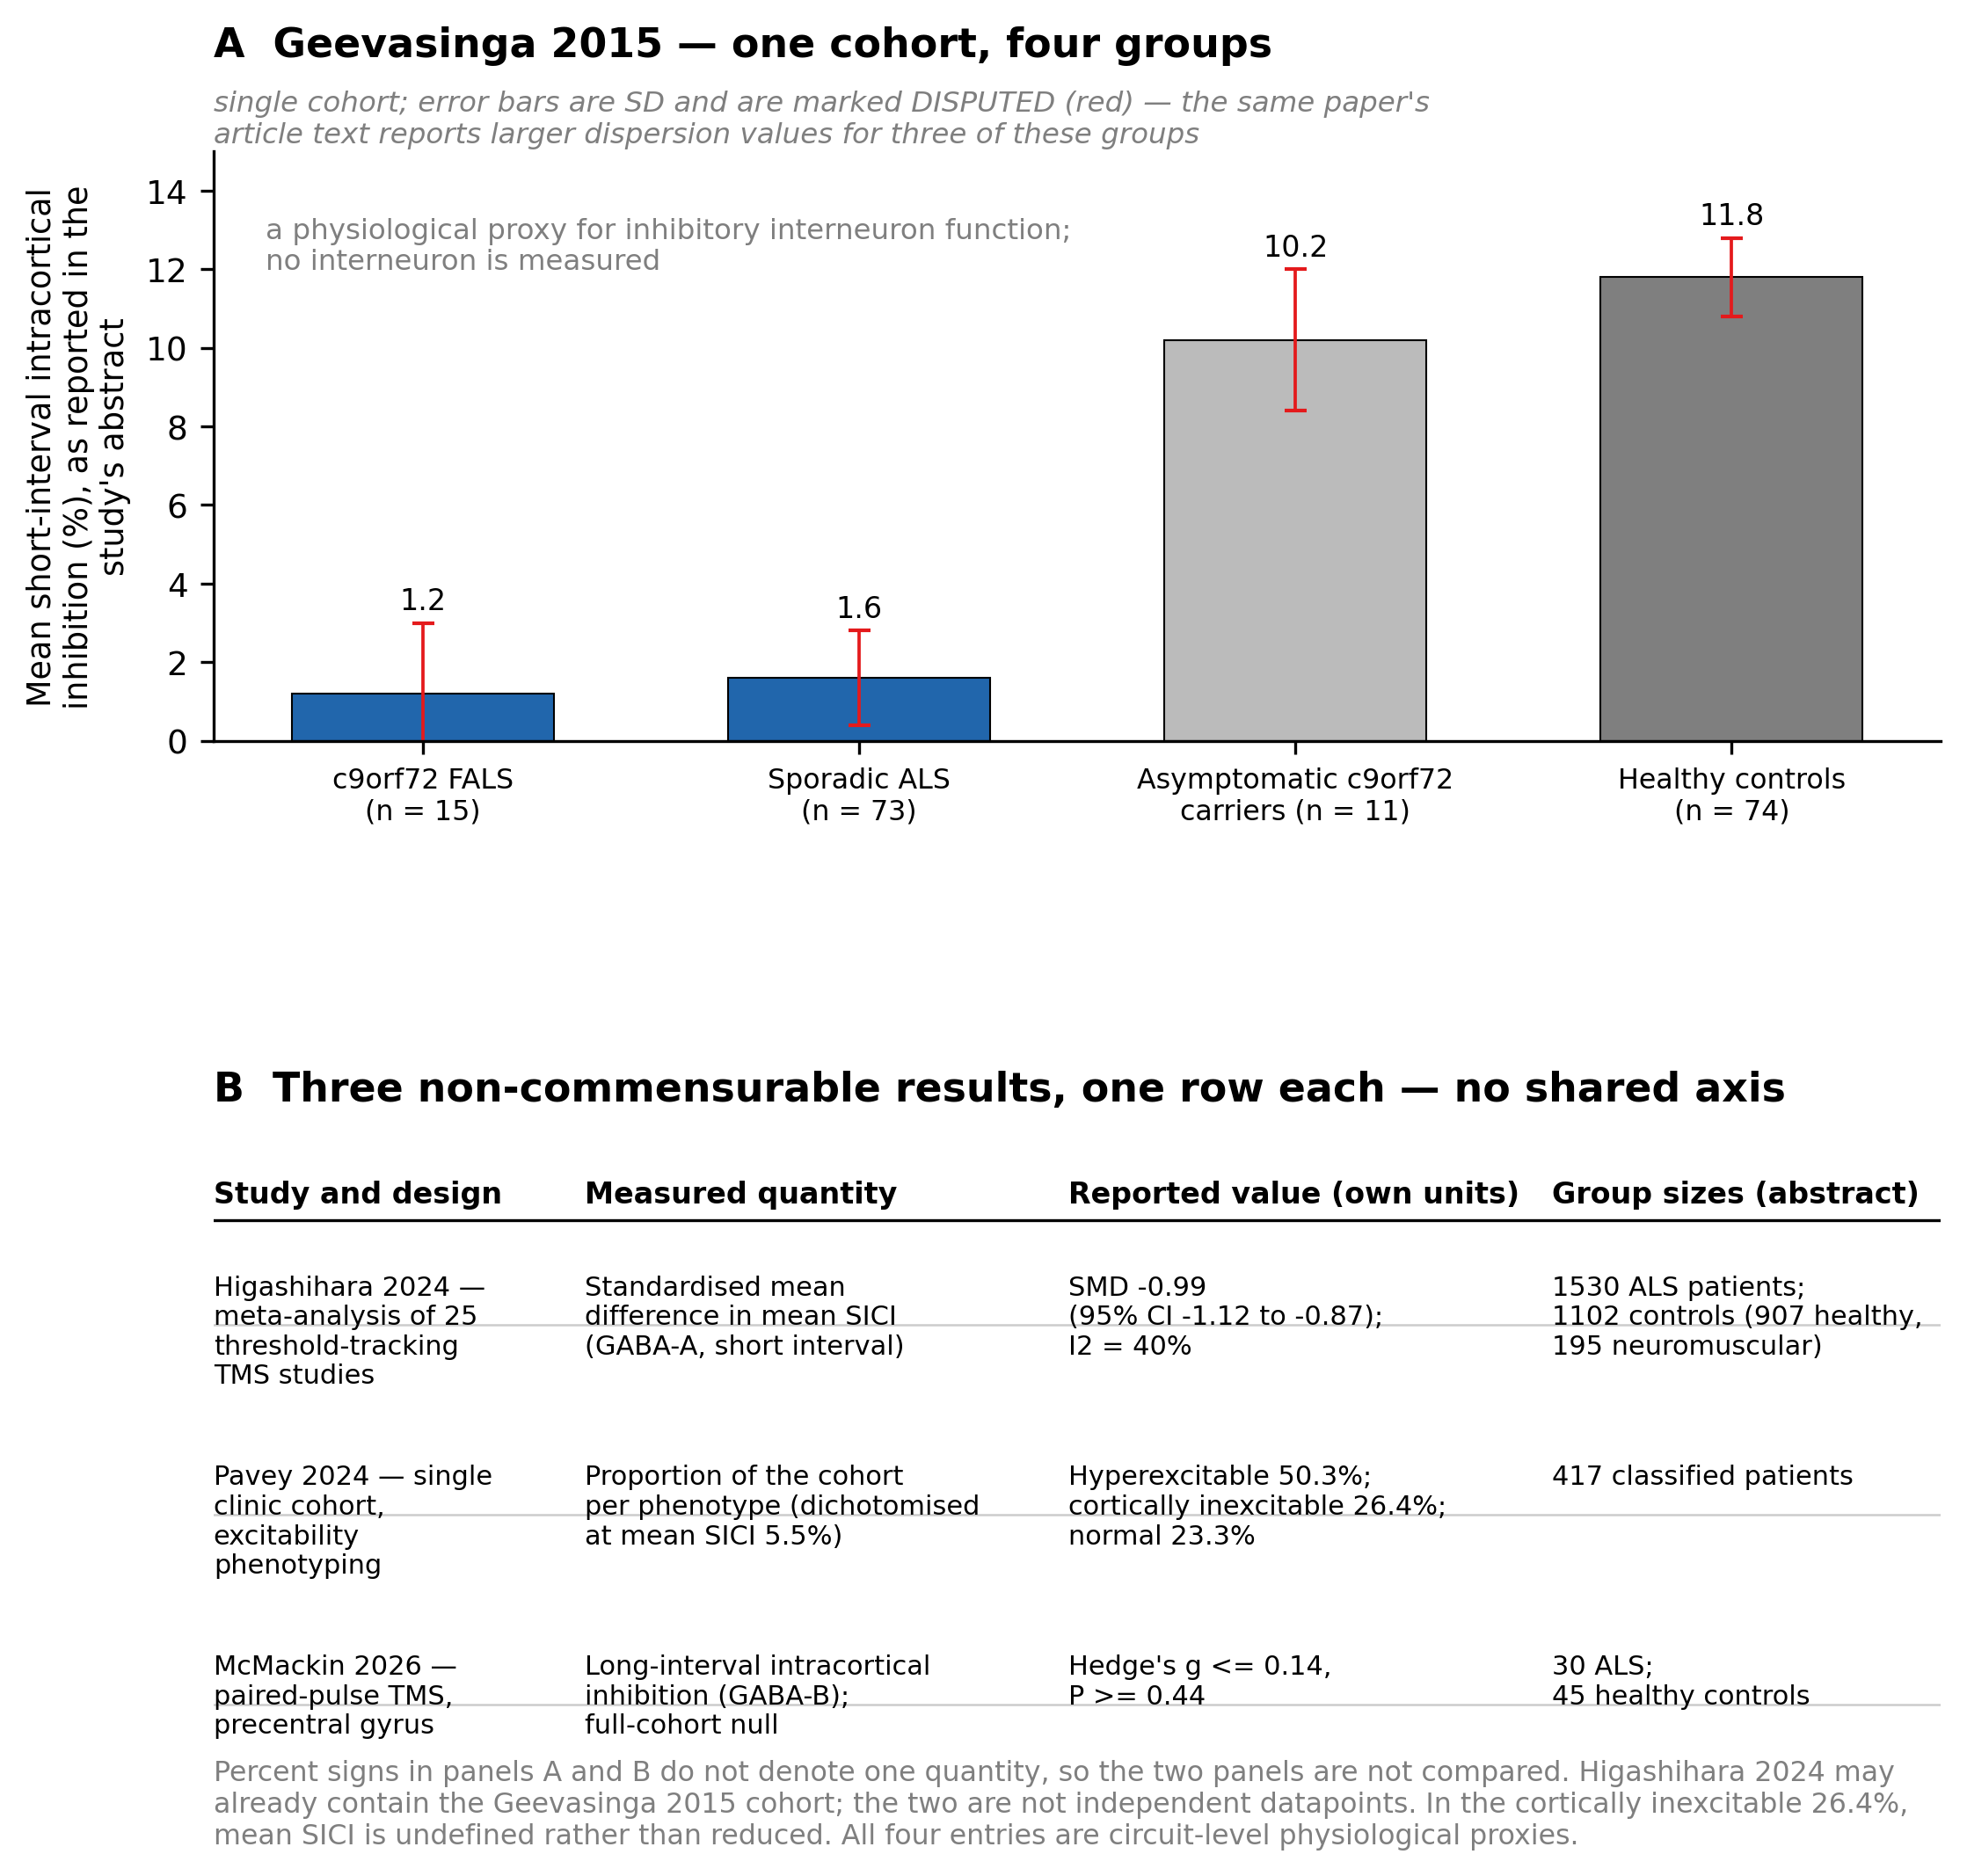
\includegraphics[width=\linewidth]{../figures/fig_sec7_cortical_inhibition_across_als_cohorts.png}
\caption{\textbf{Transcranial magnetic stimulation measures of cortical inhibition in ALS, on separate axes.} Panel A plots the mean short-interval intracortical inhibition of one cohort by group, as reported in that study's abstract; panel B is a units-explicit table of three non-commensurable results, one row each, with no shared axis. Percent signs in this figure do not denote one quantity: Geevasinga 2015 reports mean SICI amplitude (\%), whereas Pavey 2024 reports the proportion of a patient cohort in each excitability phenotype (\%), which is why they are on separate panels and are not compared. Panel A's error bars are the standard deviations reported alongside those means in the study's abstract (1.8 / 1.2 / 1.8 / 1.0). The same paper's article text reports a different set of dispersion values for three of these groups --- "patients with FALS, 1.2\% [7.0\%]; patients with SALS, 1.6\% [10.3\%]; control participants, 11.8\% [8.6\%]" --- and which set is correct cannot be determined here, so the error bars are marked disputed and the separation between groups must not be read as tight. Higashihara 2024 is a standardised mean difference pooled over 25 studies and may already contain the Geevasinga 2015 cohort, so the two are not independent datapoints; its pooled comparator is not healthy-only, since of 1102 controls 907 are healthy and 195 have neuromuscular disease, and its n counts participants pooled across 25 studies rather than studies. McMackin 2026 measures GABA-B-mediated long-interval inhibition and reports its abstract's full-cohort null (Hedge's g $\leq$ 0.14, P $\geq$ 0.44), whereas all other entries measure GABA-A-mediated short-interval inhibition; the value shown is that full-cohort result, not the study's spinal-onset subgroup analysis. That protocol spans interstimulus intervals of 50, 100, 150 and 200 ms and, by the paper's own framing, intervals below 100 ms index spinal rather than cortical inhibition, so the null is not a pure cortical measure. Pavey 2024's proportions are a dichotomisation of mean SICI at a 5.5\% threshold; in the cortically inexcitable 26.4\%, SICI is undefined rather than reduced, so that subgroup is not evidence of reduced inhibition. All four entries are circuit-level physiological proxies and none measures somatostatin or parvalbumin interneurons directly. Group sizes are taken from each paper's abstract (Geevasinga 2015: 15 C9orf72 familial ALS, 11 asymptomatic carriers, 73 sporadic ALS, 74 controls; Higashihara 2024: 1530 ALS patients and 1102 controls across 25 studies; Pavey 2024: 417 patients; McMackin 2026: 30 ALS and 45 controls), and no weighting across panels is implied. The abstracts available for this figure name no recording muscle for Geevasinga 2015; McMackin 2026's abstract specifies stimulation of the precentral gyrus and names no muscle. Sources: \citep{Geevasinga2015,Higashihara2024,Pavey2024,McMackin2026}.}
\label{fig-sec7-cortical-inhibition-across-als-cohorts}
\end{figure}

\subsection{Prion disease, Down syndrome and traumatic injury: loss of cells, or loss of markers and nets}
\label{sec-07-markers-and-nets}

These literatures are included here not because they are neurodegenerative in the same sense but because each one ran, in a model system, the experiment that the ALS and FTLD literature has not: it measured a marker and something else in the same tissue, extending the insult-specific vulnerability pattern of \ref{sec-selective-vulnerability} --- an experiment no FTLD, prion or trauma study in human tissue was retrieved as having performed. In prion disease the two measurements disagree. Severe, early and selective loss of cortical PV-positive GABAergic neurons with calbindin and calretinin subpopulations preserved is reported in scrapie and Creutzfeldt-Jakob disease (CJD) \citep{Guentchev1998}, with alteration of the PV-positive population reported in sheep scrapie, in which the extracellular matrix was examined and found unchanged \citep{Vidal2006}, and early destruction of the perineuronal net around PV interneurons in CJD, interpreted as possibly causing their loss \citep{Belichenko1999}. But in ME7 prion-infected mice the perineuronal net is progressively lost in parallel with microglial activation while the PV interneurons themselves survive through 20 weeks post-inoculation \citep{Franklin2008}, and prion aggregates are under-represented in GABA-positive neurons and concentrated in excitatory ones (p < 0.01) \citep{Erdenebat2024}, with the prion protein gene expressed roughly twofold higher in excitatory vGluT2+ neurons than in GABAergic cell types in a fatal familial insomnia model \citep{Bauer2022b} --- a single-model translatome result, flagged here as unreplicated, whose direction nonetheless converges with the aggregate distribution reported by \citet{Erdenebat2024}. Both disagreements --- reduced PV-immunoreactive density against the under-representation of prion aggregate in GABAergic neurons, and PV cell loss against perineuronal-net loss with intact counts --- are unresolved, and both turn on species, stage and whether PV immunoreactivity falls before the cell dies. The one SST-resolved measurement in prion disease is transcriptional: translating-ribosome profiling in pre-symptomatic fatal familial insomnia and CJD models reports SST neurons as showing the most prominent gene expression changes of the profiled subtypes \citep{Bauer2022a}, a preprint result awaiting replication.

Post-traumatic cortex produces the same dissociation with better controls. Controlled cortical impact depletes PV-immunoreactive interneurons in peri-injury cortex by 71\% while leaving SST interneuron and excitatory neuron numbers intact \citep{Nichols2018}, yet in the deafferentation undercut model PV and GABA immunoreactive cell counts are preserved (50.4 $\pm$ 2.7 against 50.1 $\pm$ 4.0 per section, p = 0.96) while the total NeuN cell count falls and perisomatic VGAT immunoreactivity drops by 46\% and VGAT/synaptophysin by 67\% \citep{Gu2017} --- partially resolved as a difference between injury models, but only if one accepts that counts and terminals can move independently. \citet{Folweiler2020} make that case directly: after lateral fluid percussion injury, dentate PV interneurons fail to be recruited by feedforward excitation, with evoked action potential probability falling from 57.8 $\pm$ 6.3\% to 12.0 $\pm$ 4.0\% (p = 0.0008, Glass's d = 3.6) even though the total dentate PV cell count is not significantly changed (p = 0.067) --- a significant loss in that study being confined to the hilus (p = 0.028) --- and the deficit is reversed by blocking GABA-A receptors --- excessive inhibition of the interneurons, not their loss. On the SST side, surviving cells are demonstrably not quiescent: they receive increased excitatory input after pilocarpine status epilepticus \citep{Halabisky2010}, are reported to sprout axons in an mTOR-dependent manner, although the recorded axon-crossing counts are indistinguishable between control, vehicle-treated and rapamycin-treated mice and are not normalised to the smaller surviving interneuron population \citep{Buckmaster2011}, acquire de novo excitatory input from granule and CA3 cells after controlled cortical impact and become hyperactive (43.33 $\pm$ 11.97\% responding sites after CA3 photostimulation, p = 0.0033) \citep{Butler2017}, switch L-type calcium channel subunits from CaV1.2 to CaV1.3 contralateral to injury as early network hyperactivity resolves \citep{Ihbe2021}, and reorganise their presynaptic inputs brain-wide \citep{Frankowski2022} --- an unreplicated tracing result. Their synaptic target makes this consequential: of the 42 symmetric synapses formed by one reconstructed hilar somatostatinergic axon segment, 67\% were on granule cell spines that also receive an excitatory contact \citep{Buckmaster2002} --- a single reconstruction, not a population estimate. Against these functional accounts, per-cell parvalbumin expression and gamma power fall six weeks after repetitive mild TBI \citep{MacMullin2020}, enhancing glutamate uptake preserves both intracortical inhibition and PV interneuron measures \citep{Hameed2018}, and in human epileptogenic tuberous sclerosis cortex both SST and PV interneurons downregulate GABRA1 while only SST interneurons upregulate NKCC1 and lose maturation markers \citep{Scheper2024}. One further result argues that none of this requires a proteinopathy at all: midbrain dopamine depletion alone breaks down perineuronal nets, reduces inhibition and causes progressive PV interneuron loss in the absence of amyloid, tau or alpha-synuclein pathology \citep{Cauzzi2026} --- a 2026 report with no replication yet.

Down syndrome contributes the cleanest marker-versus-function dissociation in the same animal. Anatomical work attributes increased dentate GABAergic innervation in Ts65Dn mice to a greater number of PV basket cells, normalised by removing the third App copy \citep{Mojabi2016}, and interneuron subtype counts are increased for calbindin, calretinin, NPY and VIP in CA1 and CA3 with PV unaffected \citep{HernandezGonzalez2014}; evoked GABA release is markedly raised and normalised by environmental enrichment \citep{Begenisic2011}. Optogenetic dissection of the same model, however, finds SST- and PV-evoked inhibition of granule cells kinetically distinct and age-dependently reduced, attributing the excess inhibition to neither class \citep{Gutmann2026} --- an unresolved disagreement between anatomical terminal counts and functional synaptic measurements (SST-evoked IPSC decay 55.82 $\pm$ 2.66 ms in euploid against 62.62 $\pm$ 2.65 ms in trisomic mice). For SST specifically the trisomic literature is itself split: reciprocal pyramidal-to-Martinotti connections are strengthened with larger unitary EPSCs and increased release probability at dendritic inhibitory synapses \citep{ZorrillaDeSanMartin2020}, a single-laboratory result unreplicated in six years, while triplicated miR155 suppresses SST+ interneuron production in human induced pluripotent stem cell organoids and deleting the extra copy restores their number \citep{Zhu2026}. Gene-dosage mechanisms around the same cells have been mapped in three single studies, none independently reproduced in the retrieved record --- DSCAM dosage sets GABAergic bouton number \citep{Liu2023}, the DSCAM-PAK1 pathway impairs interneuron oxidative phosphorylation \citep{Xu2022}, patient-derived lines generate fewer calretinin interneurons \citep{Huo2018} --- and maternal choline supplementation restores parvalbumin neuron number in the basal forebrain (medial septum and vertical limb of the diagonal band) to near-euploid levels (a 1.5-fold increase, 2309.71 $\pm$ 157.62 against 1584.00 $\pm$ 196.58, p = 0.001) \citep{Gautier2023} --- projection neurons rather than the cortical and hippocampal interneurons the rest of this paragraph counts, which shows the deficit is modifiable without settling what it is.

\subsection{Multiple sclerosis: four modalities, four answers}
\label{sec-07-multiple-sclerosis}

MS is where the direction of the inhibitory deficit depends entirely on the level of the GABAergic system being measured. Edited magnetic resonance spectroscopy finds lower GABA+ in posterior cingulate cortex (p = 0.036) and left hippocampus (p = 0.039) in relapsing-remitting patients, with no magnitude reported and a null in medial prefrontal cortex \citep{Cao2017}; 7T spectroscopy finds higher voxel GABA associated with smaller cortical lesion volume in the same voxel ($-$0.71 log(mm$^{3}$) per unit GABA, 95\% CI $-$1.24 to $-$0.18, p = 0.01), an association within patients rather than a patient-versus-control contrast \citep{Madsen2024}; and CSF parvalbumin at diagnosis is reported as higher in patients who are severely cognitively impaired four years later (p = 0.033), although the group means quoted in that report run in the opposite direction to the stated result and are therefore not used here \citep{Ziccardi2024}. Against the transmitter-deficit reading, \citet{Kang2020} measured cortical GABA-A receptor availability with [11C]flumazenil positron emission tomography and found global cortical binding higher in MS than in controls (5.72 $\pm$ 0.91 against 4.70 $\pm$ 0.41, p = 0.002). Receptor upregulation compensating for a reduced transmitter pool is as consistent with these data as a graded inhibitory failure --- the conflict is partially resolved in that sense, because the two modalities index different levels and the opposition may be methodological rather than biological, and \ref{fig-sec7-gabaergic-measures-in-ms-by-modality} therefore arranges the four results by level rather than adjudicating between them. The tissue literature adds a further split in the same disease: PV interneuron density falls in motor cortex \citep{Magliozzi2021,Clements2008}, and total interneuron loss in temporal cortex is 43.4\% greater in layer IV and 54.3\% greater in layer VI beneath subpial lesions than in non-lesional cortex, without subtype resolution \citep{Nicholas2015}, while demyelinated hippocampi show increased numbers of GAD67-positive neurons and elevated astrocytic GAD67 \citep{Kiljan2019}, a contested result pointing the other way.

\begin{figure}[H]
\centering
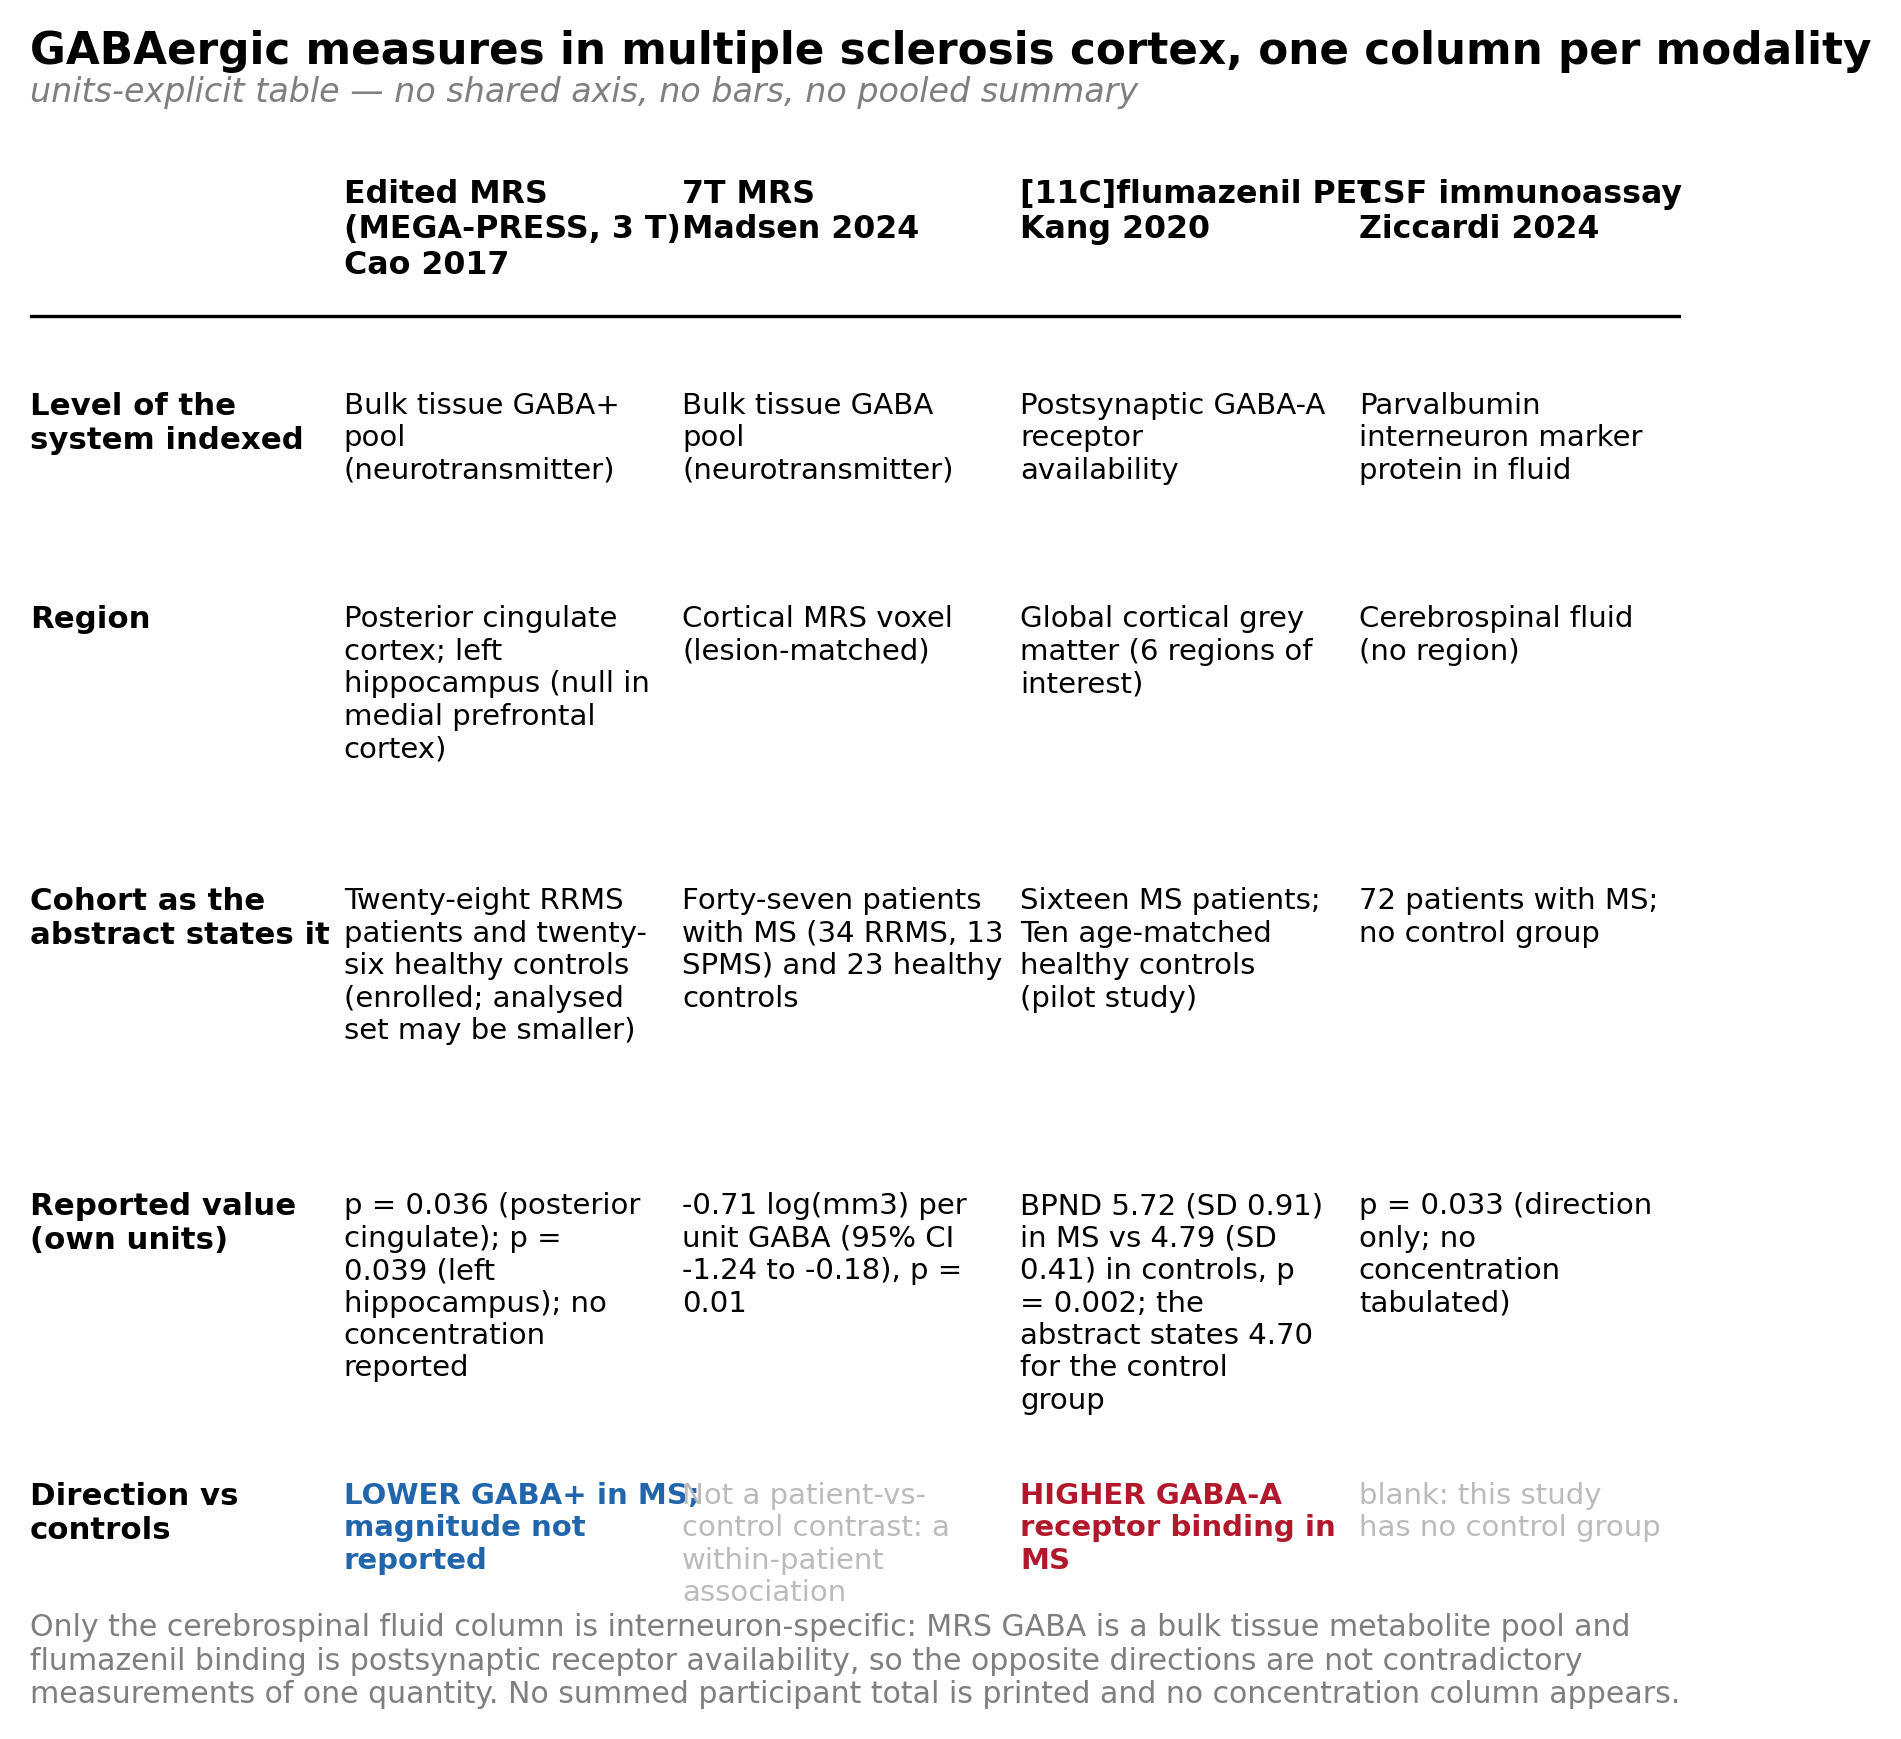
\includegraphics[width=\linewidth]{../figures/fig_sec7_gabaergic_measures_in_ms_by_modality.png}
\caption{\textbf{GABAergic measures in multiple sclerosis cortex, one column per modality.} The figure is a units-explicit table, not a grouped bar chart: there is no shared axis and no pooled summary. These four results cannot be expressed in common units --- p-values from edited spectroscopy, a regression slope in log(mm$^{3}$) per unit GABA, a unitless positron emission tomography binding potential, and a direction-and-significance statement for a cerebrospinal fluid protein --- and no concentration column appears in the table. Direction is not shared: spectroscopy indicates lower GABA in multiple sclerosis while flumazenil positron emission tomography indicates HIGHER GABA-A receptor binding. Only the cerebrospinal fluid parvalbumin column is interneuron-specific; spectroscopy GABA is a bulk tissue metabolite pool and flumazenil binding measures postsynaptic receptor availability. Ziccardi 2024's report quotes group means whose assignment contradicts the direction stated in the same sentence and in that study's abstract; the contradiction cannot be resolved from the material available, so no concentration is tabulated and the column reports only the abstract-supported direction (higher cerebrospinal fluid parvalbumin at diagnosis in patients later severely cognitively impaired) with p = 0.033. Ziccardi 2024 includes no control group --- all 72 participants are patients with multiple sclerosis and the contrast is between those later severely cognitively impaired and those later cognitively normal --- so the direction-relative-to-controls cell is left blank for that column. Kang 2020 is a pilot study (sixteen patients and ten age-matched healthy controls) and its control binding potential differs between its article text (4.79) and its abstract (4.70), so the patient-versus-control gap depends on which anchor is used. Participant counts are printed as the papers state them: Cao 2017 twenty-eight relapsing-remitting patients and twenty-six healthy controls (enrolled; no post-exclusion analysed count is available here, so the analysed set may be smaller); Kang 2020 sixteen patients and ten age-matched healthy controls; Madsen 2024 forty-seven patients with multiple sclerosis (34 relapsing-remitting, 13 secondary progressive) and 23 healthy controls; Ziccardi 2024 72 patients. No summed participant total is printed. Madsen 2024's $-$0.71 log(mm$^{3}$) coefficient is an association estimated in the patients only, so its denominator is the patient group as the abstract states it, not the whole sample, and the column is a within-patient association between voxel GABA and cortical lesion volume rather than a patient-versus-control difference. Cao 2017 contributes significance only (p = 0.036 posterior cingulate, p = 0.039 left hippocampus) with no GABA+ concentration and a null in medial prefrontal cortex, so no magnitude can be read from that column. Sources: \citep{Cao2017,Madsen2024,Kang2020,Ziccardi2024}.}
\label{fig-sec7-gabaergic-measures-in-ms-by-modality}
\end{figure}

\subsection{Scope discipline: what belongs in a somatostatin review}
\label{sec-07-scope-discipline}

The breadth of this section should not be mistaken for breadth of SST evidence. Direct, cell-resolved SST measurements in the conditions covered here exist only in rodent models and one human stem-cell model --- the TDP-43 cortical recordings \citep{Zhang2016}, the wobbler counts \citep{NietoGonzalez2010}, post-insult hippocampal counts and tracing \citep{Mishra2015,Frankowski2022,Levenga2013,Drake2024}, tau-bearing survivors in a transgenic rat \citep{Morrone2022}, trisomic Martinotti physiology \citep{ZorrillaDeSanMartin2020}, trisomic dentate SOM interneuron physiology \citep{Gutmann2026} and prion translatome profiling \citep{Bauer2022a}, with SST+ interneuron production counted in human iPSC-derived cortical organoids \citep{Zhu2026} --- plus transcript and tissue work that measures the population outside degenerating human cortex: downregulated somatostatin transcripts in bovine brainstem \citep{Krull2025}, SST+ cell counts in human tuberous sclerosis surgical cortex \citep{Scheper2024}, and a post-mortem human thalamic single-nucleus atlas quantifying the depletion of two inhibitory populations \citep{Trujillo2026}. Prion disease, MS and traumatic injury enter this review as controlled comparisons for the marker problem, not as established SST pathologies: their human evidence is dominated by parvalbumin and perineuronal net markers, and no direct quantification of SST interneurons in human prion disease, MS cortical lesions or chronic traumatic encephalopathy was retrieved. Chronic traumatic encephalopathy in particular is discussed here only through experimental traumatic brain injury models; title and abstract searches combining it with somatostatin, parvalbumin or interneuron returned no records, so the inhibitory-circuit evidence commonly attributed to that condition belongs to the injury models and not to the tissue. These absences are statements about what these searches retrieved --- one dominant full-text index without citation chasing, roughly a third of the records behind this section abstract-only, and disconfirming searches capped rather than exhaustive --- and not proof that the studies do not exist. Four disease literatures have now produced the same four explanatory axes: what was measured, where, in which construct, and in which cohort. Those disagreements are inventoried in \ref{sec-conflicts-limitations}. \ref{sec-circuit-consequences} changes the level of description and asks what SST dysfunction does to circuits, which is where the apparently contradictory cellular findings here --- hyperactive survivors, intact counts with degraded terminals, markers that fall before cells die --- become reconcilable rather than merely contradictory.

\section{Circuit Consequences: Dendritic Inhibition, Oscillations, Sleep, and Memory}
\label{sec-circuit-consequences}

The cellular descriptions assembled in \ref{sec-alzheimers} through \ref{sec-als-ftd} --- Alzheimer's disease, the Lewy body disorders, Huntington's disease and the ALS-FTD spectrum --- do not agree about what happens to somatostatin-expressing interneurons in a degenerating brain: interneurons scored as hyperactive in one amyloid model and as hypoactive in another \citep{MelgosaEcenarro2026,Meftah2026}, and a falling somatostatin-immunoreactive density in ageing cortex set against stereology that finds no change in SST+ cell number in a transgenic model \citep{Ouellet2014,Futacsi2025}. Read as competing accounts of one cell they cannot all be right; read as inputs to a circuit most of them converge, because what propagates downstream is not how many somatostatin-immunoreactive somata a section contains but how much inhibition reaches distal pyramidal dendrites and how precisely it is timed \citep{Yao2025,Udakis2020}. SST interneurons are described as roughly half of the GABAergic population and as primarily targeting dendritic compartments; in dentate gyrus their input to adult-born granule cells produces mixed inward and outward synaptic responses that betray electrotonically distant release sites \citep{Groisman2020}, and dendritic SST inhibition is routinely described as gating the integration of proximal and distal inputs and thereby pyramidal gain \citep{Taxidis2025} --- a formulation whose primary demonstrations are cited secondhand rather than shown, and which is treated here as a prevailing model to be tested rather than as a settled result. The dendritic targeting and the VIP-SST-PV motif established in \ref{sec-sst-identity} are the mechanism; what follows is what measurably breaks when it weakens, and which cellular contradictions survive translation into a circuit prediction.

\subsection{The dendritic signature: what SST manipulation does that PV manipulation does not}
\label{sec-08-dendritic-signature}

The functional signature underwriting the circuit argument comes from three preparations measuring three different quantities, and it is weaker in one respect than usually reported. Sustained photoinhibition of SST+ interneurons reliably decreased cholinergically induced slow gamma power in ventral hippocampal CA3 ex vivo, to 0.69 $\pm$ 0.057 of the baseline period (t = 5.40, p < 0.001, one-sample t test) \citep{Antonoudiou2020}. That study reports that disrupting either PV+ or SST+ interneuron activity reduces slow gamma power, but the sentence carrying the measurement quantifies only the SST+ arm, so the frequently repeated claim that SST silencing reduces gamma \emph{more} than PV silencing is weaker than its repetition suggests. Where the two classes were measured against each other with the same readout, the perisomatic class won: in prefrontal cortex in vivo, wide-spiking units were suppressed with an index of 0.39 $\pm$ 0.02 on SST activation (n = 25 units) against 0.50 $\pm$ 0.01 on PV activation (n = 22 units; P < 0.0001, unpaired t test), and peak suppression arrived later for SST than PV cells (9.92 $\pm$ 0.29 ms versus 6.73 $\pm$ 0.28 ms) \citep{Liu2020b}. Chemogenetic inactivation in frontal cortex reproduces that asymmetry: PV+ inactivation changed peak membrane potential during hippocampal input by 4.19 $\pm$ 0.98 mV against -2.39 $\pm$ 1.23 mV in controls, whereas SOM+ inactivation produced 0.66 $\pm$ 0.94 mV \citep{Zhang2024b}. A null completes the dendritic reading: potentiation of SST inhibitory synapses left action-potential generation from Schaffer-collateral stimulation essentially unchanged (0.53 $\pm$ 0.04 against 0.5 $\pm$ 0.08 after SST-iLTP, n = 8 cells, p > 0.05) \citep{Udakis2020}, and suppressing SST cells during the critical period raised inferred pyramidal spike rates without altering input tuning \citep{Yaeger2019}. Weaker, slower and invisible at the spike threshold is what dendritic targeting predicts, not evidence that SST cells matter less; \ref{fig-sec8-dendritic-versus-perisomatic-signature} sets the three quantities out panel by panel.

\begin{figure}[H]
\centering
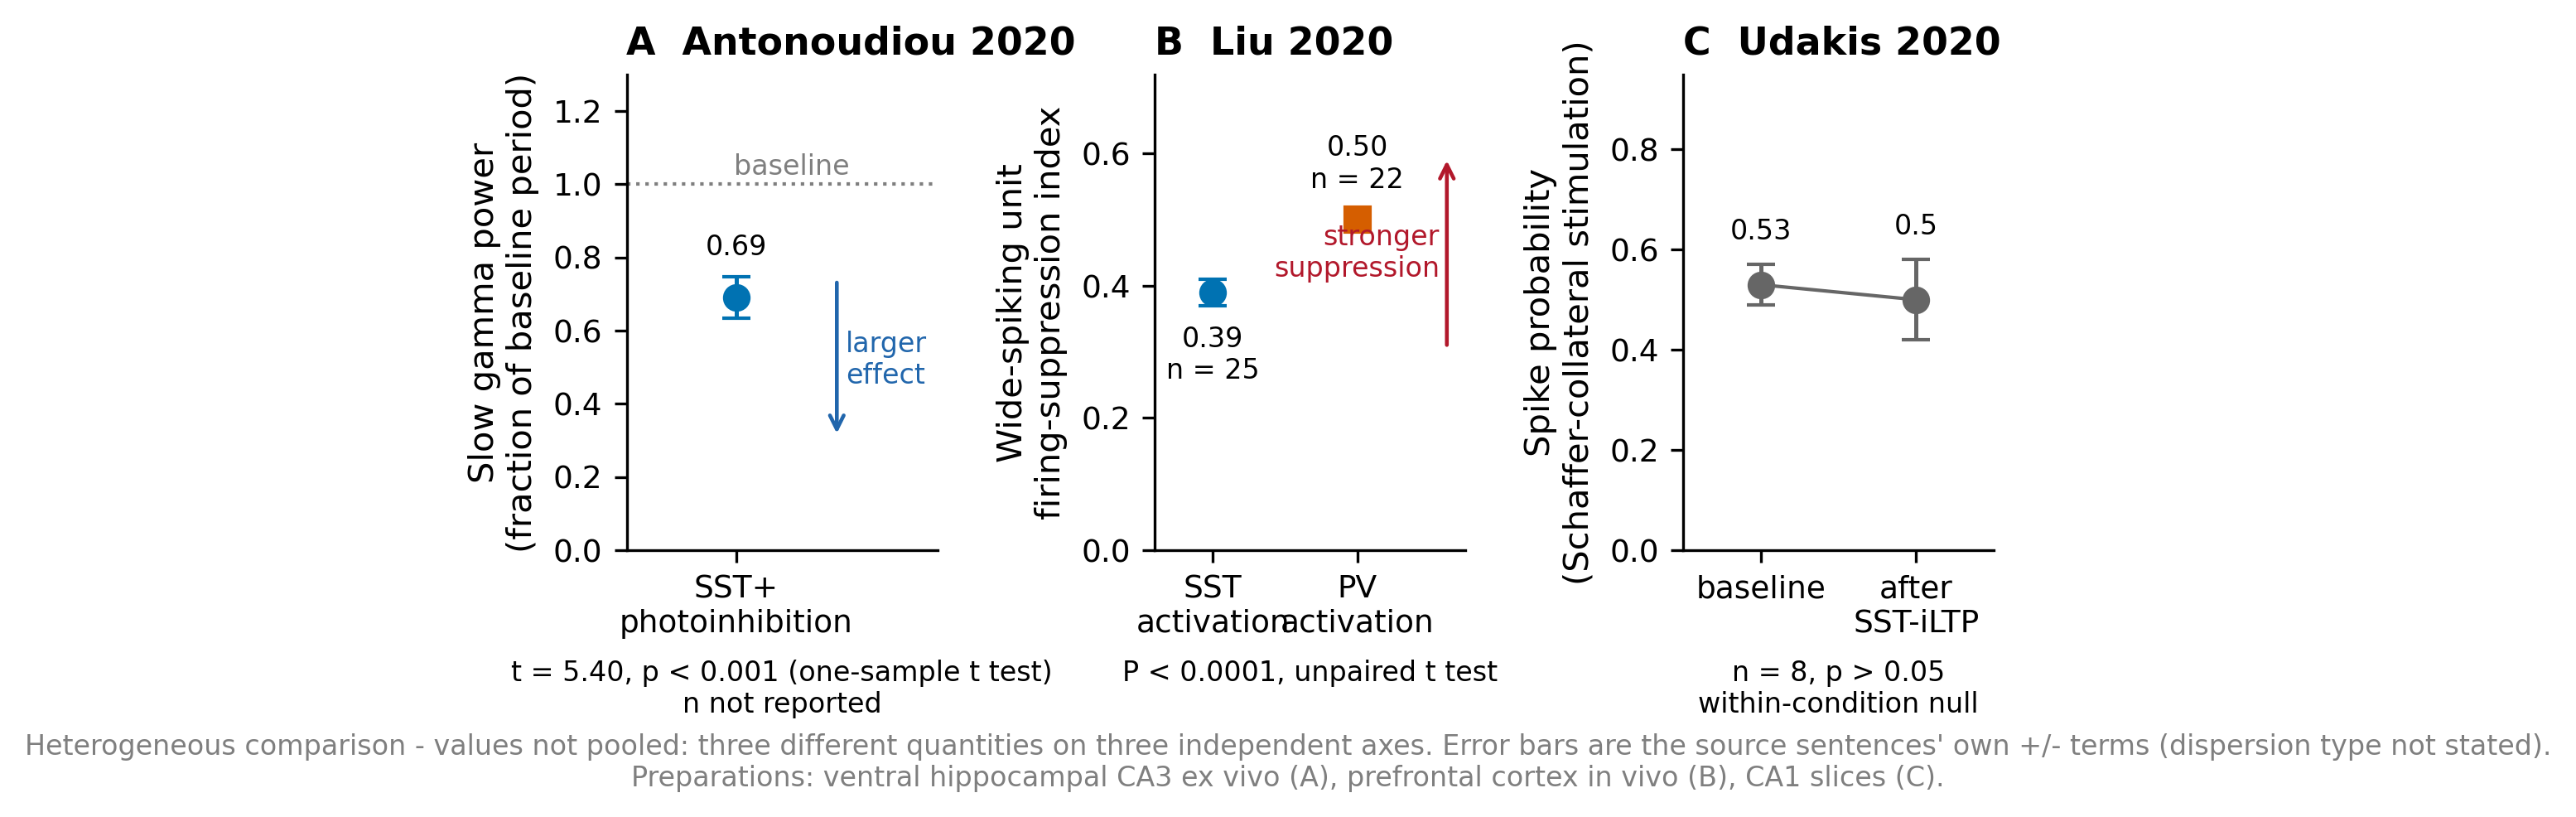
\includegraphics[width=\linewidth]{../figures/fig_sec8_dendritic_versus_perisomatic_signature.png}
\caption{\textbf{Three quantities, three preparations.} (A) Slow gamma power during SST+ interneuron photoinhibition, as a fraction of the baseline period: 0.69 $\pm$ 0.057 (t = 5.40, p < 0.001, one-sample t test) \citep{Antonoudiou2020}. (B) Wide-spiking unit firing-suppression index on SST versus PV interneuron activation: 0.39 $\pm$ 0.02 (SST, n = 25) and 0.50 $\pm$ 0.01 (PV, n = 22); P < 0.0001, unpaired t test \citep{Liu2020b}. (C) Spike probability from Schaffer-collateral stimulation before and after SST-iLTP: 0.53 $\pm$ 0.04 versus 0.5 $\pm$ 0.08 (n = 8, p > 0.05) \citep{Udakis2020}. Caveats carried with this figure: \citet{Antonoudiou2020} recorded cholinergically induced slow gamma in ventral hippocampal CA3 ex vivo. The three panels are three different quantities (fraction of baseline gamma power; dimensionless firing-suppression index; spike probability) plotted on separate axes and must not be read as a common scale. Index polarity is not shared: in panel A a smaller value means a larger effect of SST photoinhibition, whereas in panel B a larger suppression index means stronger suppression; panels A and B each carry an explicit direction-of-effect arrow, and panel C carries none because it is a null within-condition comparison for which no direction is claimed. Only panel B is a quantified SST-versus-PV contrast --- \citet{Antonoudiou2020}'s source sentence reports no number for the PV arm, so no PV value is plotted in panel A, and the absence of a PV bar must not be read as an absent PV effect, since that study reports that disrupting either PV+ or SST+ interneuron activity reduces slow gamma power. Panel C is a within-condition comparison in the same cells and is a null result, not an SST-versus-PV contrast. In panel C the measured unit is the postsynaptic CA1 pyramidal cell, not a property of the SST interneuron; in panel B the measured unit is likewise the wide-spiking unit rather than the SST or PV interneuron that is optogenetically activated, the interneuron being the manipulated population in both panels. Preparations differ: ventral hippocampal CA3 ex vivo (A), prefrontal cortex in vivo (B), CA1 slices (C) --- two of three are ex vivo. The stimulation condition under which the suppression indices of panel B were obtained is not stated in the source sentence; that study's abstract reports frequency-specific optogenetic manipulations during social interaction, which does not establish the condition behind these indices. Sample sizes count different things: no sample size is stated in A, wide-spiking units per arm in B, and cells in C; each arm of panel B carries its own n.}
\label{fig-sec8-dendritic-versus-perisomatic-signature}
\end{figure}

Where and when these cells fire reinforces the compartment claim. SST cells are required for phase-locking to a context-dependent low-gamma rhythm that grows with stimulus size, peaking at 32 $\pm$ 1 Hz at 21 degrees across 32 mice \citep{Veit2017}, and their recruitment is strongly brain-state dependent: during sleep, bistratified and PV+ basket cells fired 16.9 and 19.2 Hz faster than O-LM cells (t(10) = 2.35, p = 0.0407; t(10) = 2.75, p = 0.0204) \citep{Katona2014}, an identified O-LM-like neuron was recruited by sharp-wave ripples in quiet wakefulness but not in sleep ripples \citep{Katona2017}, and a sparse long-range Sst population labelled in two intersectional lines was intensely active in slow-wave sleep and quiet wakefulness and suppressed in movement and REM, in 95 of 111 superficial-layer cells \citep{Ratliff2026}. In the dentate gyrus, putative SST cells fire last in the dentate spike sequence, at +1.5 ms after the peak against -1.5 ms for putative PV cells \citep{Hainmueller2026}, the delayed-feedback position the dendritic account requires; in anterior cingulate cortex, 13 of 21 Som neurons were suppressed at reward-zone entry \citep{Kvitsiani2013}. Superficial and deep CA1 pyramidal cells depolarise maximally at different theta phases (195 $\pm$ 32 against 222 $\pm$ 22 degrees), implying that the dendritic inhibition they receive arrives at systematically different phases of the cycle \citep{SanchezAguilera2021}. Circuit models recover the same division of labour: reducing SST inhibition in a human L2/3 microcircuit raised baseline firing by 68\% (0.72 $\pm$ 0.03 to 1.21 $\pm$ 0.03 Hz) while changing the stimulus-evoked response by 3\% \citep{Yao2025}, feedback onto SOM cells allows gain and stability to move together rather than in opposition \citep{Bos2025}, two-interneuron networks occupy multistable oscillatory regimes whose beta/gamma structure depends quantitatively on inhibitory coupling strength \citep{DeySarkar2026}, a parkinsonian motor-cortex microcircuit reproduces beta-band burst structure from an isolated reduction of layer 5 pyramidal-tract neuron excitability in an otherwise unmodified network \citep{Doherty2025}, and learning-related retuning can be reproduced by strengthening SST-to-PV connections \citep{Wilmes2019}. The convergence is real, but it is a convergence of direction and compartment, not of magnitude: almost no two of these studies measure the same quantity, and the closest pairs still differ in preparation or region.

\subsection{Oscillatory phenotypes in disease models are band- and parameter-specific}
\label{sec-08-oscillatory-phenotypes}

"Gamma deficit" is the phrase this literature uses, and it conflates amplitude with frequency. In an amyloid model, slow (30-60 Hz) gamma power was reduced (F(1,56) = 9.89, p = 0.0027, n = 6) while fast (60-120 Hz) gamma was not (F(1,56) = 0.8096, p = 0.3721) \citep{Etter2019}; normalised hippocampal gamma power fell from a z-score of 5.1 in wild-type to 1.7 in mice combining amyloid with Nptx2 deletion, with amyloid alone at 3.9 (p = 0.0199, one-way ANOVA) \citep{Xiao2017}. In a human-tau propagation model, by contrast, slow- and mid-gamma peak frequencies were indistinguishable between genotypes (28.7 $\pm$ 0.7 against 29.3 $\pm$ 1.2 Hz; 56.8 $\pm$ 0.8 against 59.3 $\pm$ 4.1 Hz), reported by the authors as similar distributions with no test statistic \citep{Viney2022}. Amyloid models also slow and desynchronise more broadly, with reduced theta-band EEG coherence across vigilance states \citep{Constantino2026} and slow-wave power reduced from three months of age while slow-wave frequency stayed at 0.6 Hz \citep{Lee2023a}, whereas a tau model is reported to decrease beta power and raise markers of cortical excitability instead, with no effect size reported \citep{Irmen2026}, and in patients resting theta elevation is topographically distinct between Alzheimer's disease and frontotemporal dementia \citep{Cai2026}. Interneuron classes are not interchangeable controllers of a single oscillatory variable either: PV-interneuron-restricted GluK1 ablation shifted hippocampal theta peak frequency from 8.78 $\pm$ 0.11 to 9.46 $\pm$ 0.12 Hz (p = 0.0007) without changing it in prefrontal cortex, though theta and gamma power were elevated in both hippocampus and prefrontal cortex in the same animals, so it is the frequency shift and not the phenotype that is region-selective \citep{Rhee2026}; potentiation at pyramidal and PV synapses raised peak low-gamma power 2.5- to 3-fold in a CA3 network model \citep{Hadler2024}; deleting GAD67 from SOM cells left slow-oscillation up-state duration intact while shortening it in PV-GAD67 mice (p = 2.3 x 10-3, N = 5) \citep{Kuki2015}, a single study with no replication in the retrieved record eleven years on; driving O-LM alpha2 cells generated a theta2 peak near 7 Hz (n = 6, p < 0.0001) \citep{Mikulovic2018}, that result and the risk-taking association built on it being unreplicated in the retrieved record eight years on; and impaired fast inhibition in a channelopathy model slowed ripples by about 21 Hz from a wild-type 235.69 $\pm$ 6.12 Hz rather than abolishing them \citep{Lascorz2026}. Optogenetic suppression of lateral-septum SST neurons, the manipulation named in that study's title and abstract, changed dorsal hippocampal theta power by 14.8\% (p = 8 x 10-7) along with ripple density \citep{Espinosa2022}, although its individual results sentences attribute the theta increase to stimulation of these cells and the fall in ripple density to silencing them. Which parameter moves identifies which element failed; pooling them loses exactly that information, which is why \ref{fig-sec8-oscillatory-phenotypes-and-manipulations} keeps power, peak frequency and the parvalbumin-side manipulations on separate axes.

\begin{figure}[H]
\centering
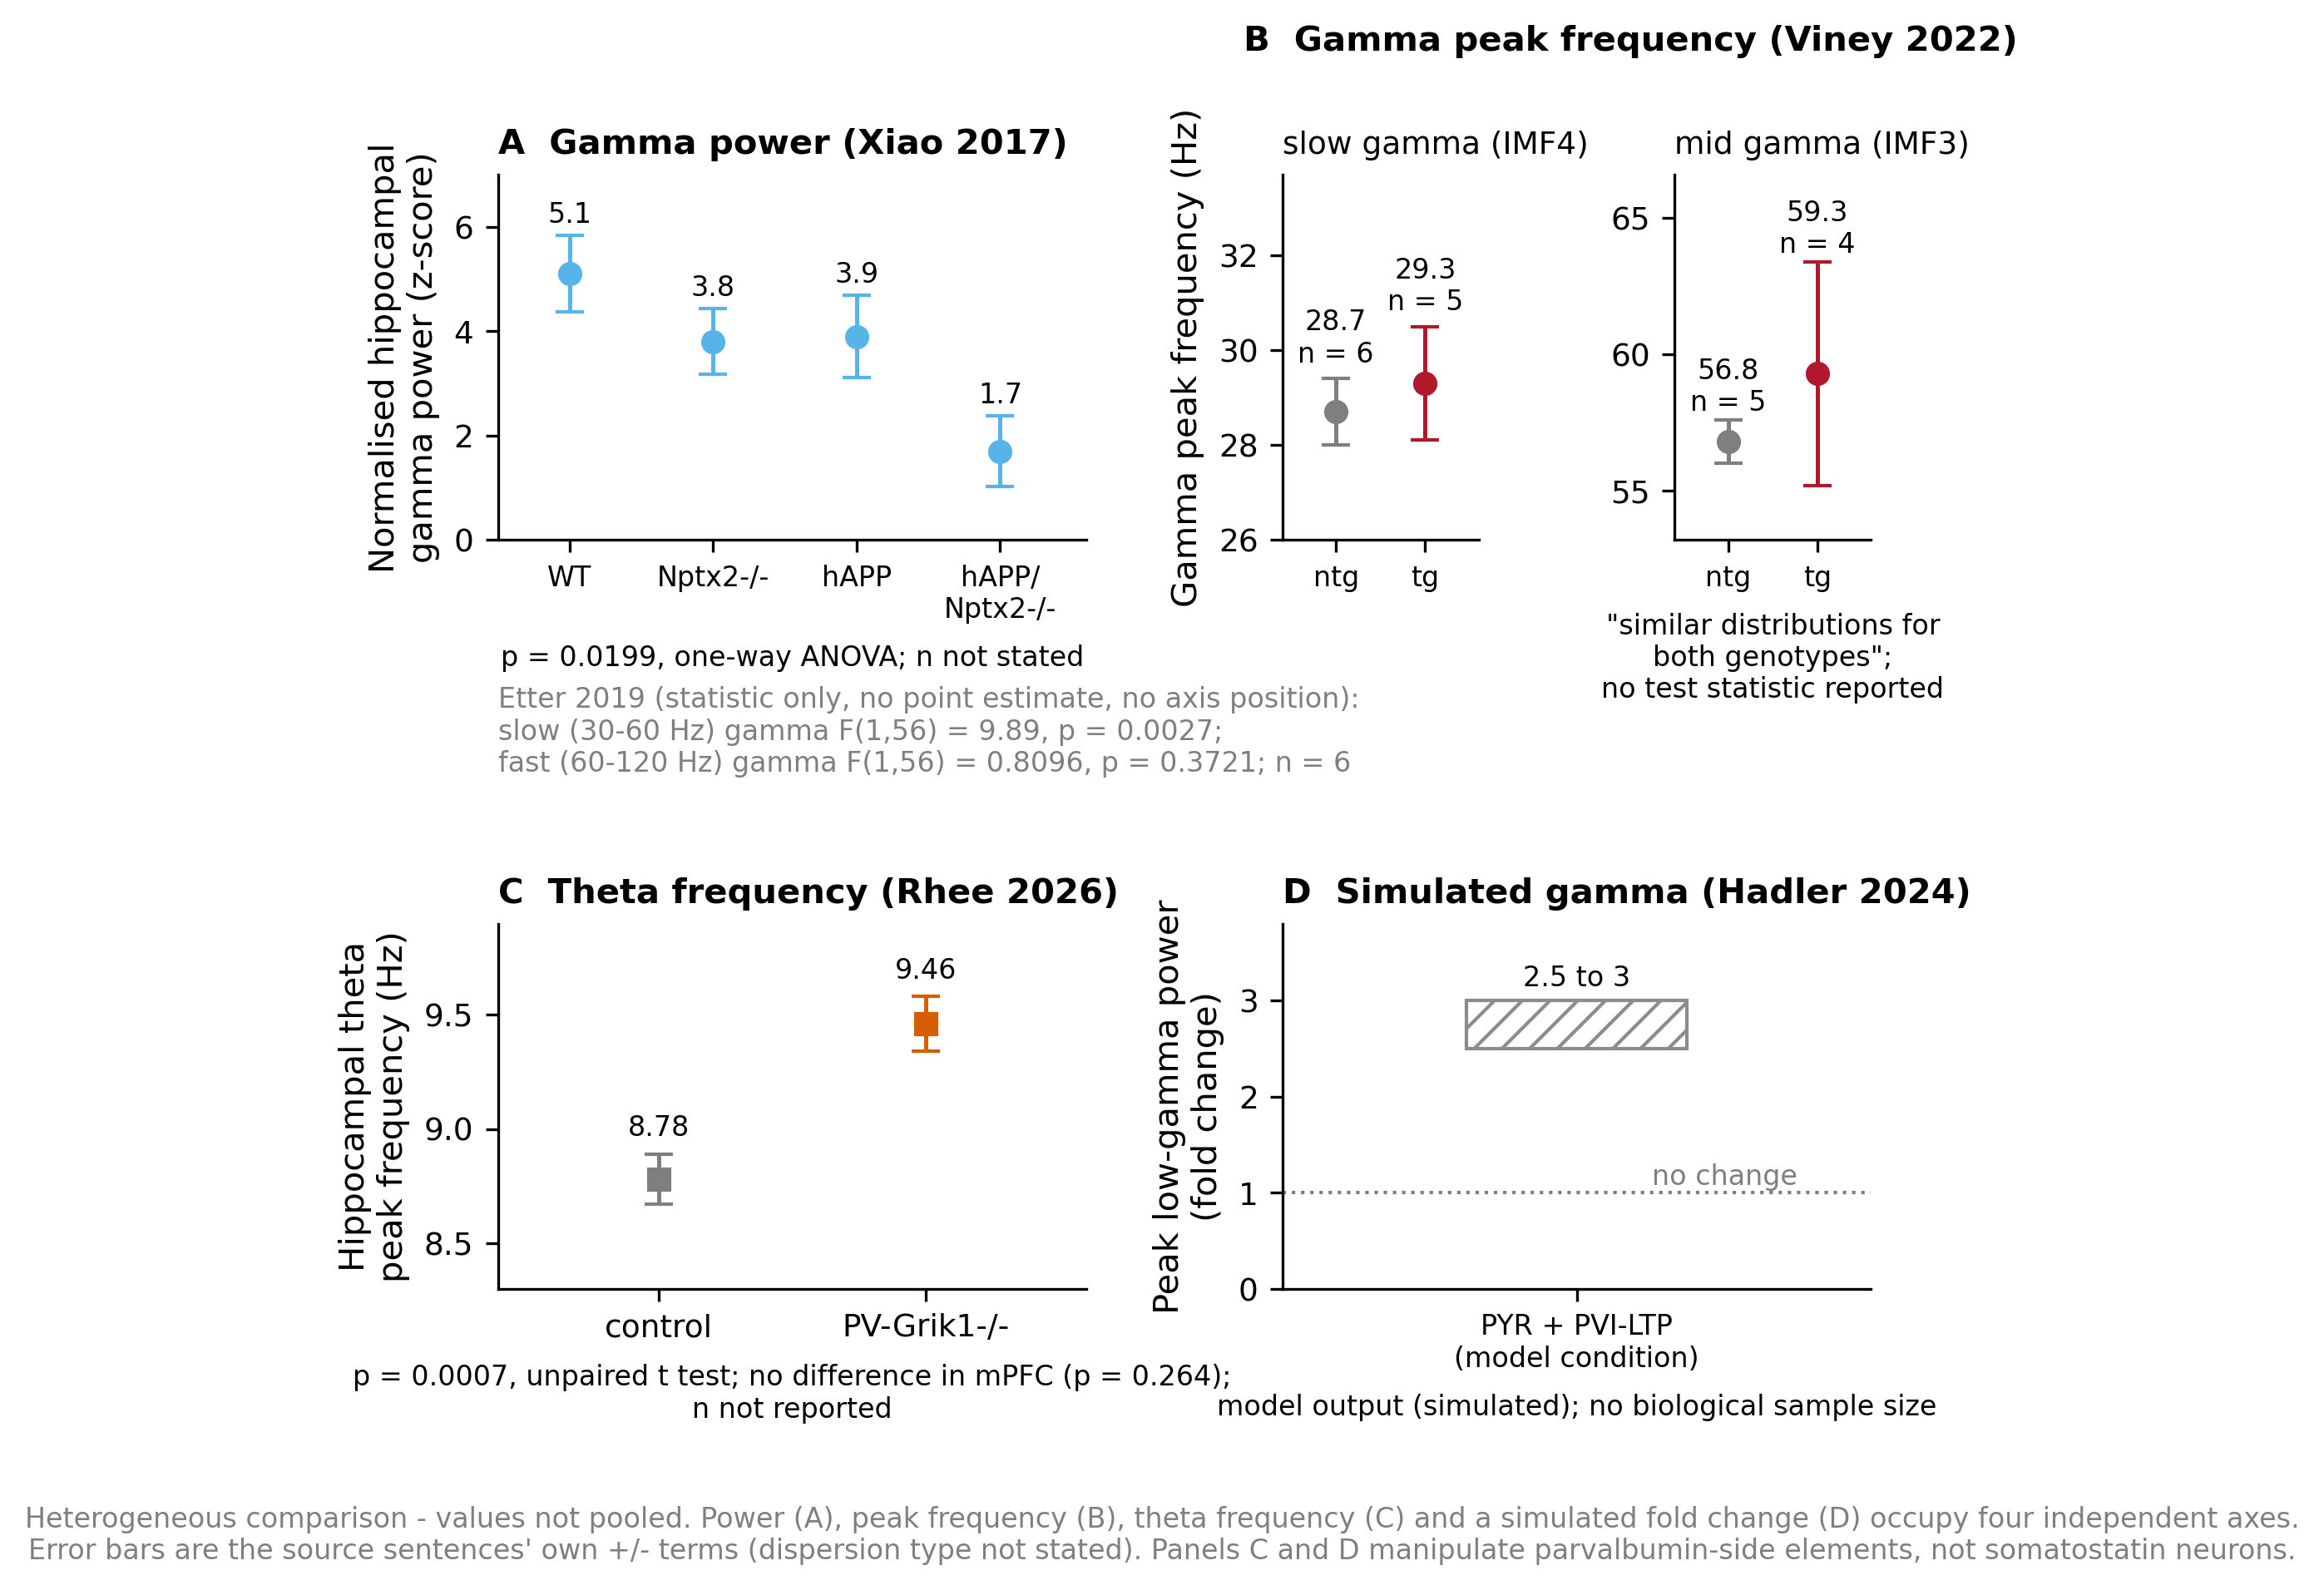
\includegraphics[width=\linewidth]{../figures/fig_sec8_oscillatory_phenotypes_and_manipulations.png}
\caption{\textbf{Power, frequency, and which element was manipulated.} (A) Normalised hippocampal gamma power (z-score) by genotype \citep{Xiao2017}, with the slow- versus fast-gamma genotype statistics of \citet{Etter2019} printed as a statistics row. (B) Slow- and mid-gamma peak frequency in a tauopathy model, plotted on band-local axes \citep{Viney2022}. (C) Hippocampal theta peak frequency in control and PV-Grik1-/- mice \citep{Rhee2026}. (D) Peak low-gamma power fold change, a model-condition output \citep{Hadler2024}. Caveats carried with panels A and B: all four genotype groups of \citet{Xiao2017} are shown because the gamma-power reduction is carried by the hAPP/Nptx2-/- double mutant (1.7), whereas amyloid alone (hAPP, 3.9) sits near the Nptx2-/- single mutant (3.8) and below wild-type (5.1), so the value is not attributable to amyloid alone. \citet{Etter2019} contribute a genotype main effect only (F and p); no point estimate exists in the source, so this entry is drawn as a statistics row with no position on the power axis, not a bar. Recording-site grain is unresolved on one side only: \citet{Xiao2017} recorded extracellular field potentials from stratum pyramidale of CA3, whereas the subfield and layer of \citet{Etter2019}'s hippocampal recording are not stated in the source sentence or abstract supporting this value; gamma power is layer-dependent, so the two sites may not be read as equivalent. \citet{Xiao2017} state no n in the source sentence or abstract, and their preparation is ex vivo, acute hippocampal slices from 3--4-month-old mice, while \citet{Etter2019} state n = 6 without specifying whether this is per genotype; \citet{Etter2019}'s study also applies optogenetic stimulation and the source sentence does not state the stimulation condition under which the genotype comparison was measured. \citet{Xiao2017}'s model is hAPP crossed to Nptx2-/-, with the APP line named in that study's Methods as APPswe/PS1dE9; the line behind the other amyloid entry is not named in the source sentence or abstract supporting its value, so the two amyloid models are not established to be the same line. \citet{Viney2022} report "similar distributions for both genotypes" and give no test statistic for the genotype comparison, so panel B is annotated with that wording and not as "n.s."; animal numbers differ per band (slow gamma, n = 6 non-transgenic and n = 5 transgenic; mid gamma, n = 5 and n = 4); this is a tauopathy model (THY-Tau22) whereas panel A shows amyloid models, so disease mechanism and time course differ; the behavioural state behind these values is unresolved because the study reports both head-fixed and freely moving recordings and the source sentence does not say which contributed them; the recording subfield is not named in the source sentence or abstract supporting this value; and peak frequency and power are independent properties of the gamma band, so panel B shares no axis with panel A. Caveats carried with panels C and D: neither entry manipulates somatostatin neurons --- both act on parvalbumin-side elements (a PV-interneuron-restricted GluK1 ablation; combined pyramidal-cell plus PV-interneuron potentiation) --- so this pair is the parvalbumin comparator, not an SST manipulation series. The two values are different oscillations and units (theta peak frequency in Hz; low-gamma power as a fold change) and are plotted on separate axes. \citet{Hadler2024}'s 2.5-to-3-fold value is the output of a CA3 network-model condition, not a recorded measurement, and panel D is marked as simulated. \citet{Rhee2026}'s theta peak-frequency difference is hippocampus-specific (no difference in mPFC, p = 0.264), but the same study reports elevated theta and gamma oscillation power in both hippocampus and mPFC, so panel C must not be read as showing a hippocampus-confined phenotype. The manipulations differ in kind (a PV-interneuron-restricted GluK1 ablation versus acute plasticity induction in a model); the source sentence and abstract supporting this value do not establish when the ablation takes effect, and lifelong developmental compensation is an inference drawn here rather than a finding reported by the study. Neither entry reports a sample size traceable to the sentence carrying its value, and the two "n not reported" cells are not equivalent: panel D is a model condition with no biological sample size, whereas panel C is a recording whose animal numbers are simply not stated. Error terms on the Xiao, Viney and Rhee points are the source sentences' own $\pm$ values; those sentences do not state whether they are SEM or SD, so they carry no dispersion claim.}
\label{fig-sec8-oscillatory-phenotypes-and-manipulations}
\end{figure}

\begin{quote}
\noindent\textbf{Evidence Conflict}\par
Whether the SST pathway is functionally spared in amyloid-oligomer oscillopathy is unresolved, and the disagreement is probably about which synapse was measured. Optogenetic dissection of carbachol-induced CA1 gamma in oligomer-treated slices localised the damage to reciprocal pyramidal-cell-to-PV synapses and found pyramidal-to-SST synapses intact, with desynchronised spike phases relative to gamma \citep{Park2020}. Recording in vivo from the same model, a second study found both theta (3-12 Hz) and gamma (30-60 Hz) power reduced in oligomer-injected SST-Cre mice, with increased initial GABA release probability at SST as well as PV output synapses \citep{Chung2020}. The first interrogates the excitatory input to the interneuron, the second its inhibitory output onto pyramidal cells, so both can hold; the disagreement is reconciled by what each study measured rather than by data, and no experiment in the retrieved record tests input and output of the same SST population side by side. The claim that SST interneuron loss causes network hypersynchrony in Alzheimer's disease, repeated across secondary sources, has no primary demonstration in this record that isolates SST cells from PV dysfunction or general inhibitory failure --- and one retrieved study localises amyloid-induced gamma failure to PV rather than SST synapses \citep{Park2020}.

\end{quote}

The therapeutic corollary inherits two unresolved premises. Driving fast-spiking PV interneurons at 40 Hz reduced CA1 amyloid-beta labelling intensity by 39.5\% relative to controls \citep{Iaccarino2016}; chronic 40 Hz optogenetic stimulation of cortical GABAergic interneurons in APP mice restored slow-wave activity across the 24-hour period (6 mice per group) but did not alter plaque load or microglial number \citep{Zhao2023}. The two differ in targeted population, region and stimulation duration, and the disagreement stands open. Whether sensory flicker engages native gamma circuits at all is separately contested: 40 Hz visual stimulation increased 40 Hz spectral power in wake, N2, N3 and REM \citep{Hainke2024}, but phase analysis in visual cortex showed phase angles exceeding one full cycle within the duration of the first gamma cycle (17.2 ms), indicating that even stimulation at the oscillator's own frequency does not capture its dynamics \citep{Duecker2021}. A single human session of 40 Hz audiovisual stimulation entrained scalp EEG without improving attention-network performance (alerting t(19) = -0.992, p = 0.334) \citep{Wu2025}, while older adults lacked the theta-phase-to-gamma-amplitude nesting present in younger adults (z = -0.540, p = 0.286 against z = -2.724, p = 0.003), a deficit rhythmic transcranial stimulation is reported to restore, though no effect size for the restoration itself is reported \citep{Reinhart2019}. Replication of the amyloid-lowering effect by laboratories outside the originating group was not retrieved by these searches, and the mechanism handed forward to \ref{sec-therapeutics} therefore rests on two premises each contradicted by at least one retrieved study.

\subsection{Sleep: slow oscillations, spindles, and the clearance link}
\label{sec-08-sleep}

The human sleep phenotype is the strongest bridge in this section and the one with the weakest cellular grounding. Non-rapid-eye-movement (NREM) stage-2 spindle density improved prediction of CSF total tau by delta R-squared = 0.284 above age, sex and ApoE4 genotype (p = 0.001) and was the only sleep variable to do so; the variance statistic is itself unsigned, and the direction comes from the study's own report that N2 spindle density correlated negatively with CSF total tau \citep{Kam2019}; slow-wave activity supported memory specifically in amyloid-positive older adults, classified against a PiB global DVR cutoff of 1.065 \citep{Zavecz2023}; and the overnight memory benefit of slow-wave count was fully mediated by travelling-slow-wave features (total effect beta = 0.48, 95\% CI 0.103 to 0.850, p = 0.011) \citep{Rouast2026}. Crucially these measures are modifiable. Phase-locked acoustic stimulation increased slow-oscillation-coupled spindles by 24\% in the intervention arm against 0\% in controls (t = 2.81, P = 0.01; group difference t = -2.41, P = 0.02), although that trial found no group difference in memory performance or plasma amyloid, its reported benefits resting on within-group associations between response magnitude and later memory \citep{Wunderlin2023}, slow-wave-spindle coupling strength tracked overnight plasma amyloid-beta 42/40 change on the third experimental night (beta = 2.5, p = 0.006) \citep{Wunderlin2026}, and anodal slow-oscillation tDCS raised spindle power by 24.1\% in intermediate-to-evening chronotypes, a subgroup of 10 of 22 participants whose mean change carries an SD of 72.1\% (pairwise p = 0.077; chronotype-by-stimulation interaction p = 0.068) \citep{Dikici2026}. On the model side, zolpidem restored slow-oscillation and delta power in an amyloid model relative to each animal's own baseline \citep{Yu2026}, optogenetic drive of cortical interneurons restored slow-wave activity in the same disease class \citep{Zhao2023}, and tau confined to dorsal raphe serotonin neurons reduced NREM percent delta composition (p = 0.0328) \citep{Kolling2026} --- a single study, not independently replicated in the retrieved record. These observational and interventional results are shown together in \ref{fig-sec8-sleep-oscillations-tau-and-memory}.

\begin{figure}[H]
\centering
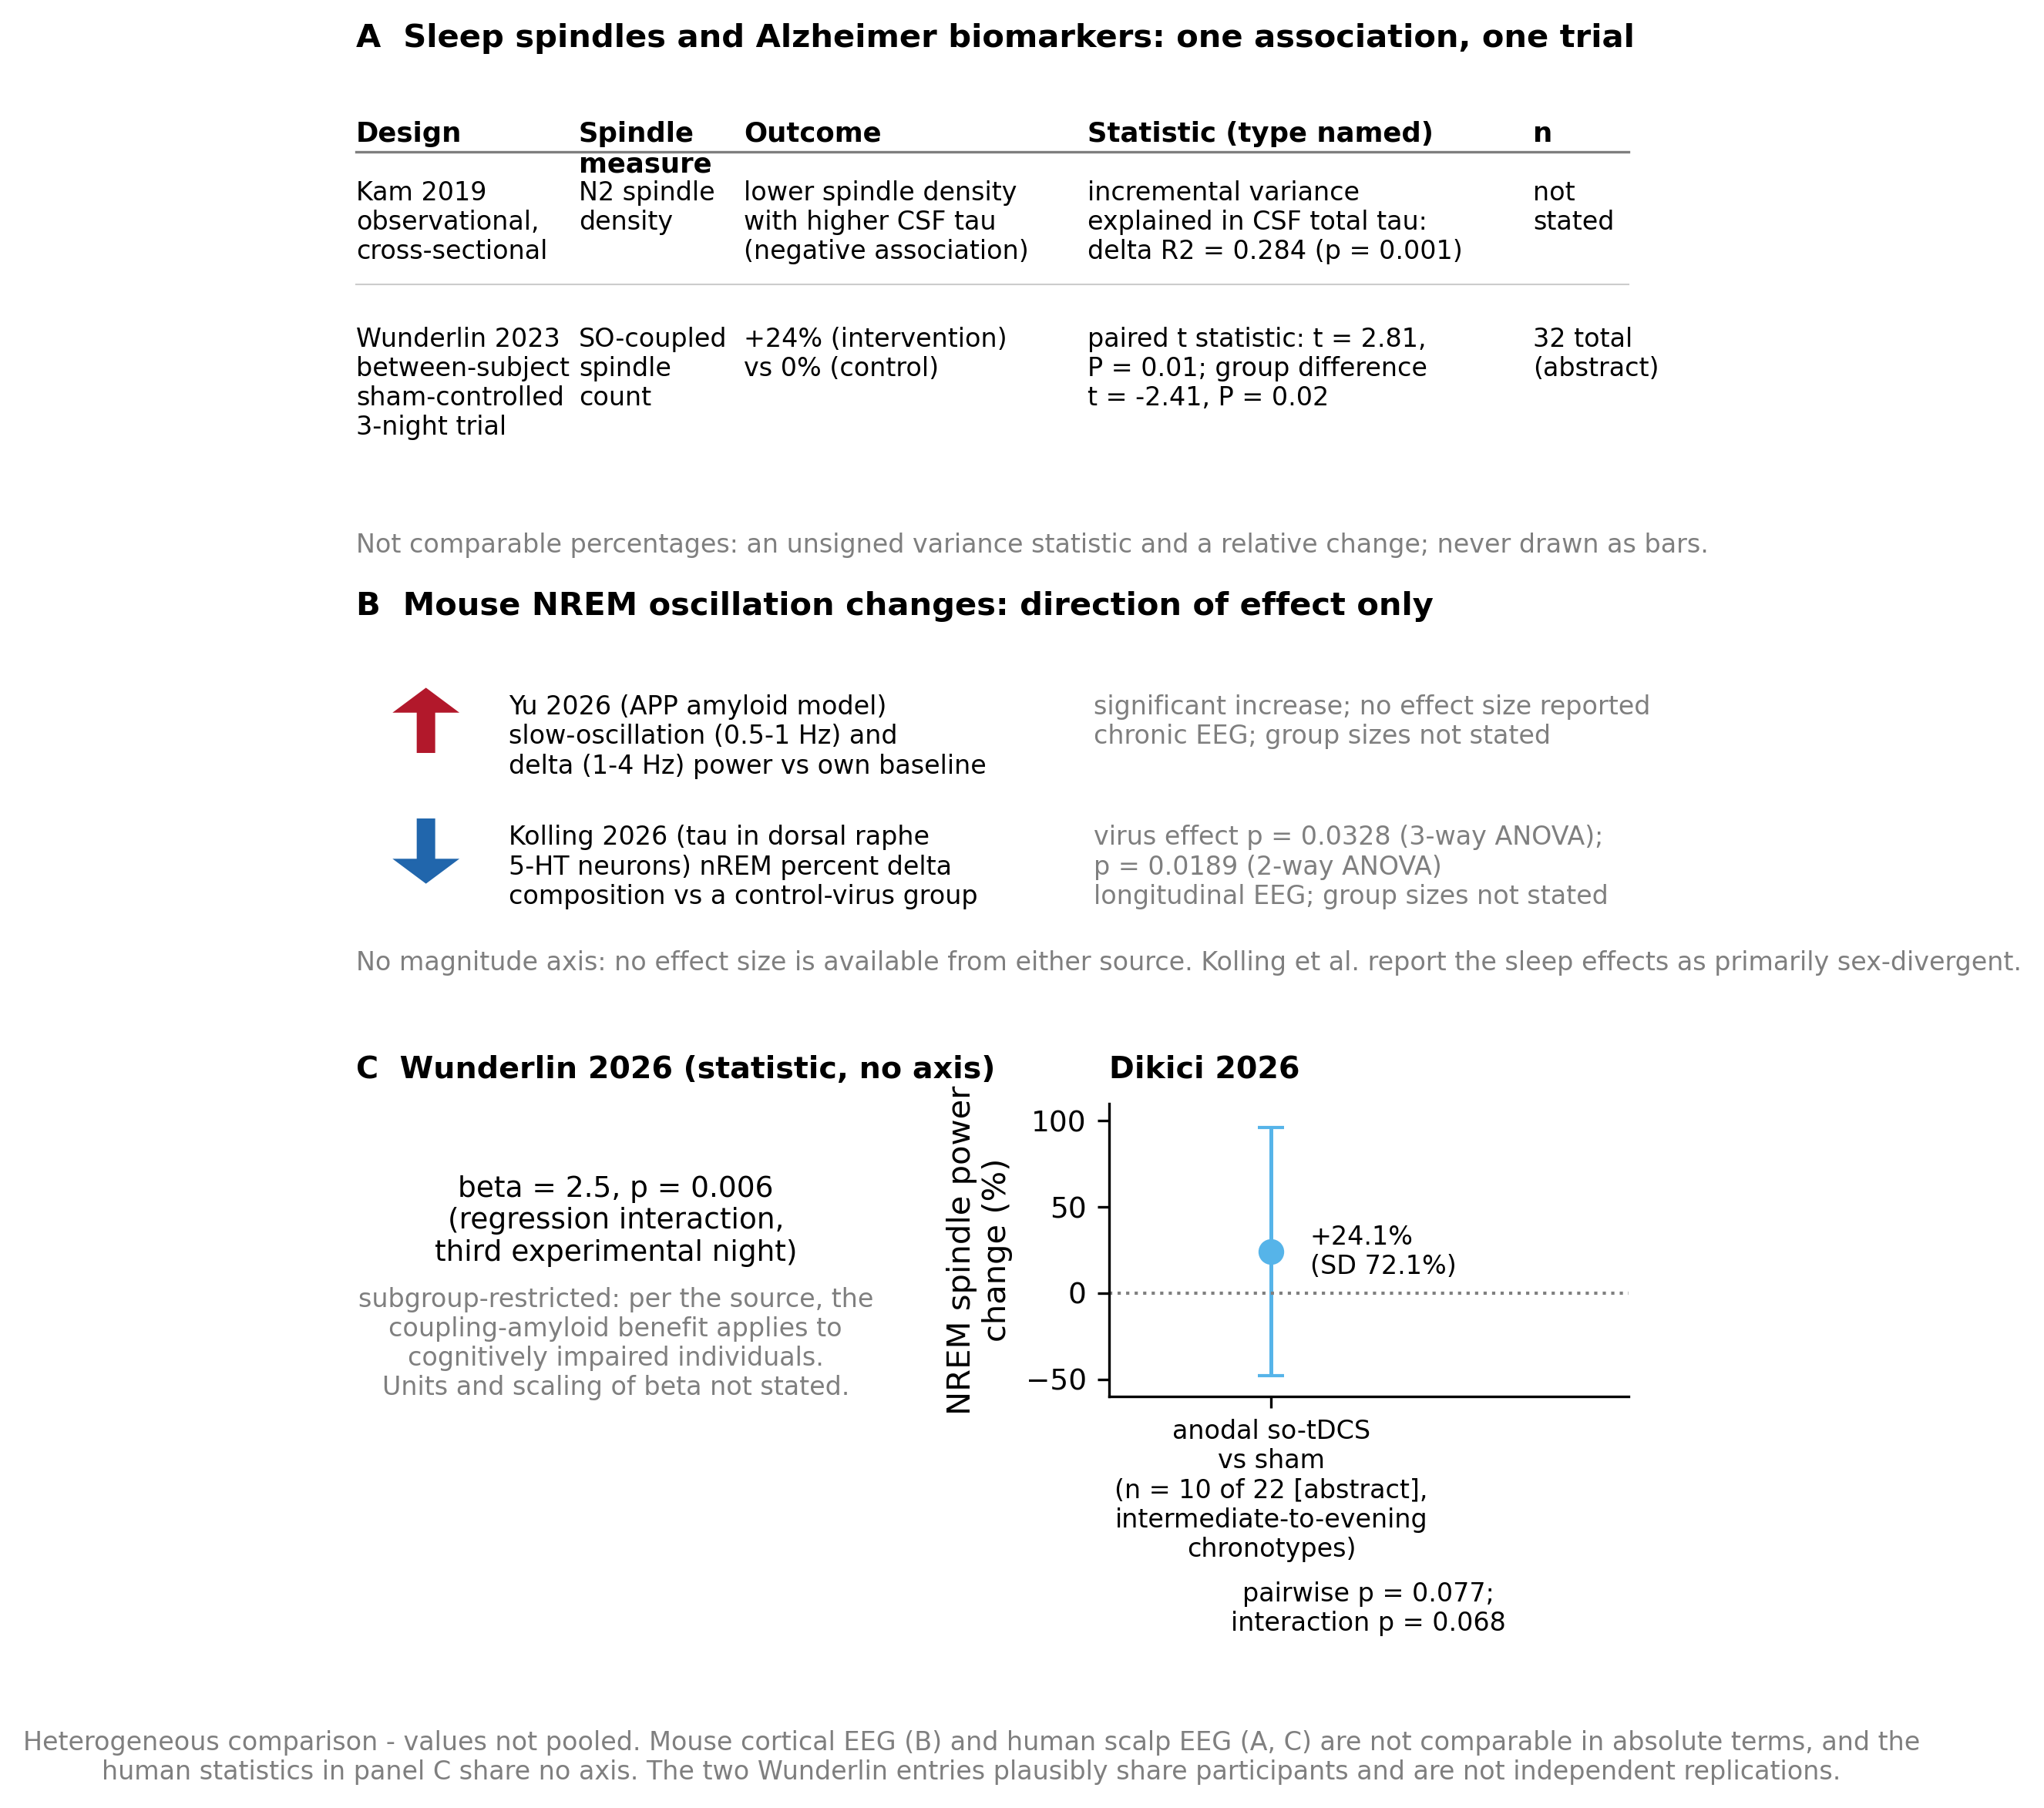
\includegraphics[width=\linewidth]{../figures/fig_sec8_sleep_oscillations_tau_and_memory.png}
\caption{\textbf{Sleep oscillations, biomarkers, and interventions, never pooled.} (A) Two spindle studies side by side as a table: an observational association of N2 spindle density with CSF total tau (delta R-squared = 0.284, p = 0.001) \citep{Kam2019} and a sham-controlled stimulation trial changing slow-oscillation-coupled spindle count (+24\% against 0\%, t = 2.81, P = 0.01) \citep{Wunderlin2023}. (B) Direction-of-effect glyphs for two mouse studies \citep{Yu2026,Kolling2026}. (C) Two human statistics, each in its own column \citep{Wunderlin2026,Dikici2026}. Caveats carried with panel A: the two values are not the same kind of quantity --- delta R-squared = 0.284 is incremental variance explained in CSF total tau and +24\% is a relative change in slow-oscillation-coupled spindle count under acoustic stimulation; they are not comparable percentages and are never drawn as bars. The direction of inference differs, one entry treating spindle density as a predictor of an Alzheimer biomarker and the other treating acoustic stimulation as a predictor of spindle coupling, and delta R-squared is an unsigned variance statistic whose underlying association in \citet{Kam2019} is negative, the opposite sign to the +24\% increase in the other row. \citet{Kam2019} is a cross-sectional association in cognitively normal older adults with CSF biomarkers; \citet{Wunderlin2023} is a between-subject sham-controlled three-night trial (32 participants) that reported no group difference in plasma amyloid or memory, while reporting within the intervention group that the magnitude of the stimulation-induced response was associated with memory up to three months later and with beneficial plasma amyloid change. Outcome matrices differ (CSF total tau versus plasma amyloid) and no shared outcome links the two rows. Neither source reports the analysed sample size in the sentence carrying its value; only the trial total of 32 is available, from the abstract, and that figure belongs to the Wunderlin row alone, so the Kam row reads "not stated". \citet{Wunderlin2023} and \citet{Wunderlin2026} plausibly share participants and must not be read as independent replications. Caveats carried with panel B: both entries contribute a direction of effect only --- no effect size is available from the cited sources --- and are drawn as up/down glyphs with their p-values, never as bars with implied magnitude; mouse cortical EEG is not comparable in absolute terms with the human scalp-EEG entries of panel C; the two manipulations differ in kind (a systemic hypnotic drug in an amyloid model versus viral tau expression targeted to dorsal raphe serotonin neurons, recorded with longitudinal EEG); \citet{Kolling2026} report the sleep effects as primarily sex-divergent, so the single glyph shown here is not a sex-resolved result and a pooled glyph averages over a declared sex interaction; the dependent variables differ (absolute slow-oscillation and delta power versus percent delta composition of nREM, a proportion rather than a power); group sizes are not stated in either source sentence; and the comparators differ, \citet{Yu2026}'s direction being relative to the animals' own pre-injection baseline and \citet{Kolling2026}'s relative to a control-virus group. Caveats carried with panel C: the two values are different statistics and each occupies its own labelled column --- a regression interaction coefficient (beta = 2.5) whose units and scaling the source does not state, printed as a statistic with no axis position, and a percentage change in spindle power (+24.1\%) on its own axis; no shared axis and no pooling. \citet{Dikici2026}'s +24.1\% is a subgroup mean (intermediate-to-evening chronotypes, n = 10 of 22) whose mean change is 24.1\% with an SD of 72.1\% as stated in the source sentence, and whose comparisons are printed on the face of the figure as the source's own statistics (pairwise p = 0.077; interaction p = 0.068) rather than as a significance mark. \citet{Wunderlin2026}'s coupling-amyloid interaction is specific to the third experimental night and, per the source, benefited amyloid response exclusively in cognitively impaired individuals, so it is marked subgroup-restricted on the face of the figure; the interventions differ in modality (three-night phase-locked acoustic stimulation versus slow-oscillatory transcranial direct-current stimulation during naps); neither source sentence states the analysed sample size for its plotted statistic beyond \citet{Dikici2026}'s chronotype subgroup (n = 10); and \citet{Wunderlin2026} pooled and re-analysed data from three clinical trials, so the two Wunderlin entries must not be presented as independent replications.}
\label{fig-sec8-sleep-oscillations-tau-and-memory}
\end{figure}

The bridge lacks its middle term. No recording or manipulation of identified cortical SST interneurons during spindle events was retrieved by these searches; searches linking somatostatin interneurons to spindles returned slow-oscillation, sleep-onset and sleep-deprivation studies instead, so the human spindle biomarker currently has no cellular interpretation. Nor is there an SST-selective sleep rescue: interventional studies in disease models drive GABAergic interneurons broadly, with opsins or with zolpidem \citep{Zhao2023,Yu2026}, and no study restoring slow-wave activity by SST-selective manipulation in a tau or amyloid model was retrieved by these searches. The indirect evidence that SST cells belong here is nonetheless substantial: brief activation of cortical Sst neurons in the ON state is described as inducing a long OFF state that silences broad cortical populations, with inhibition of those neurons reducing slow-wave activity --- a claim reaching the retrieved record through a secondary source rather than its primary demonstration \citep{Kobayashi2026}; activity-tagged prefrontal Sst neurons were sufficient to initiate nesting and subsequent NREM sleep when reactivated (light against no light, P = 0.0046 at 5 Hz, P = 0.0498 at 10 Hz and P = 0.0202 at 20 Hz; the P = 0.0297 and P = 0.0043 values that study reports belong to light-evoked action-potential probability in slice recordings), a single study awaiting replication \citep{Tossell2023}; that same superficial-layer long-range Sst population is selectively active in slow-wave sleep \citep{Ratliff2026}; five hours of sleep deprivation raised hippocampal Sst and Npy transcripts two- to fourfold against roughly 30\% for Gad67 and Pvalb \citep{Delorme2021}; and amyloid oligomers abolished the learning-induced increase in sharp-wave-ripple occurrence during post-encoding slow-wave sleep (t12 = 2.43, p = 0.032, n = 7) \citep{Nicole2016}. The human counterpart of these associations is assembled in \ref{sec-human-evidence}.

\subsection{Memory: dendritic gating of plasticity and its disease relevance}
\label{sec-08-memory}

If SST inhibition acts on dendrites rather than spike threshold, its behavioural signature should be control over what is learned rather than how much is fired --- which is what the plasticity data show. O-LM interneurons control the dendritic calcium signalling and synaptic plasticity initiated by entorhinal input to CA1 pyramidal neurons, an effect reported qualitatively, with no effect size given, while their own activity was lower on the initial laps of a novel environment than on later laps of a familiar one (0.011 $\pm$ 0.005 against 0.093 $\pm$ 0.063 $\Delta$F/F0) --- the fall in dendritic inhibition that permits the plasticity new place fields require \citep{Udakis2025}; the same inhibition terminates plateau potentials with a steep dependence on timing within the plateau (20 $\pm$ 6.7\% termination at 10 ms against 62.7 $\pm$ 7.7\% at 50 ms; n = 17, Friedman chi-square = 42.8, p < 10-8) \citep{Vaasjo2026}. The receptor-level mechanism offered for this gating is alpha5-subunit GABA-A-mediated control of synaptic NMDA-receptor activation, with slow dendritic IPSCs reduced 29.4 $\pm$ 7.1\%, from 138.8 $\pm$ 23.3 to 95.9 $\pm$ 14.6 pA, by an alpha5-selective negative allosteric modulator (n = 6, P < 0.01) \citep{Schulz2018} --- a single study, unreplicated in the retrieved record eight years on. Dendrite-targeting layer 1 interneurons strongly reduced apical dendritic calcium responses across 130 recorded dendrites and themselves underwent learning-related potentiation \citep{Abs2018}, motor learning drove spine formation specifically in distal apical branches in layer 1 \citep{Chen2015}, and systemic ketamine (10 mg/kg) reduced SST somatic calcium event rates by 13 $\pm$ 3\% against a 13 $\pm$ 6\% increase with saline, while dendritic spine event rates rose 43.42 $\pm$ 0.01\% against 4.34 $\pm$ 0.01\% \citep{Ali2020} --- co-observed changes under a drug with many other actions, and another single-laboratory demonstration. Behaviourally, SST activation during the early delay of a working-memory task impaired performance strongly, as did PV activation, while VIP activation improved it \citep{Kamigaki2017}, prefrontal SST activation alone raised freezing above baseline in the absence of the conditioned stimulus, mimicking a conditioned response \citep{Cummings2019}, and chemogenetic activation of dentate SST cells impaired object-location encoding (p = 0.0047) and retrieval (p = 0.046) but not consolidation (p = 0.8804) \citep{Raven2026}. In an amyloid model, remote memory decline was accompanied by increased inhibitory input onto prefrontal engram cells without altered PV reactivation \citep{VanAdrichem2025}, and driving O-LM alpha2 cells generated type 2 theta, which that same unreplicated study associates with increased risk-taking in response to predator odour \citep{Mikulovic2018}. Two gaps bound this account: the in vivo demonstrations are slice and head-fixed preparations rather than freely behaving animals, and no human tissue or in vivo human evidence for dendrite-targeted inhibitory gating of plasticity was retrieved, so every statement here about human dendritic inhibition crosses species without a bridging measurement.

\subsection{Reconciling the cellular contradictions at circuit level}
\label{sec-08-reconciliation}

The cellular disagreements need not be settled for the circuit prediction to hold, which is both the strength and the limit of this account. Whether SST cells in amyloid cortex are hyper- or hypoactive is open: immediate-early-gene labelling found c-Fos elevated at both PV and SST neurons in App knock-in cortex relative to wild-type (two-way ANOVA, p < 0.001), with the increase reported as relatively greater at PV cells \citep{MelgosaEcenarro2026}, whereas awake silicon-probe recording in young APP/PS1 mice found fast-spiking interneurons shifted towards low firing rates with pyramidal cells unchanged \citep{Meftah2026}; model construct, age and readout all differ, and no retrieved study measures SST and PV firing with the same awake electrophysiological readout in both knock-in and transgenic models at matched ages. Activity is in any case spatially graded rather than uniform, SOM interneurons within 60 micrometres of plaques being more active than distant ones (Kruskal-Wallis H(2) = 18.41, p < 0.0001) \citep{Algamal2022a}. Whether the population is numerically reduced is equally open: somatostatin-immunoreactive density in rat auditory cortex fell to 0.9 $\pm$ 0.3 cells per high-power field into old age with a further \textasciitilde{}20\% rise in NPY immunostaining \citep{Ouellet2014}, whereas unbiased stereology in young TgF344-AD rats could not observe any change in the numbers of PV+, calretinin+ or SST+ neurons \citep{Futacsi2025}, the counting-method axis of the same disagreement examined for the striatum in \ref{sec-huntingtons} and for the cortex in \ref{sec-alzheimers}, so driver, age, region and counting method are all confounded with the outcome, and head-to-head stereology across amyloid, tau and synucleinopathy models at matched ages does not exist in this record.

Each of these cellular states predicts the same circuit failure. Developmental ablation reducing CA1 SOM+ neurons by 46.41\% \citep{Subramanian2024} and inflammatory downregulation of Sst, Cort and Npy transcripts that BDNF infusion prevents \citep{Rezaei2025} both reduce effective dendrite-targeted inhibition, and both therefore predict degraded low-gamma synchronisation and degraded NREM coordination without requiring a single SST neuron to die. Two neighbouring perturbations make that prediction less tidy rather than confirming it. Deleting the GABA-A gamma2 subunit from SST cells disinhibits those cells and increases their intrinsic excitability and spike output \citep{Fuchs2016}, which moves dendrite-targeted inhibition in the opposite direction, so what this family of manipulations predicts in common is dysregulated rather than uniformly weakened dendritic inhibition. The region-restricted interneuron loss recorded in Lewy body cingulate cortex but not inferior temporal gyrus is a parvalbumin-density measurement \citep{Hawksworth2026}, a perisomatic rather than a dendrite-targeting population, and it therefore speaks to where inhibition fails regionally rather than to whether the dendritic compartment is the one affected. This is why a disease can present a severe somatostatin phenotype with the cells still present, and why the account is hard to falsify: what would distinguish these states is not a cell count but a compartment-resolved measurement --- dendritic inhibitory conductance or plateau-potential termination probability measured in the same preparation as low-gamma power and NREM slow-oscillation-spindle coupling, with SST cells identified independently of somatostatin expression. Such an experiment must also resolve which SST cells it addresses: O-LM cells are a highly homogeneous transcriptomic population across Sst-Cre and Htr3a-Cre lines, the one Cre-line-dependent expression difference being attributed by that study to the BAC copy of Htr3b in the Htr3a-Cre line rather than to a molecular split \citep{Winterer2019}, their overlap with the somatostatin population differs between subiculum and CA1 (59 $\pm$ 2\% against 47 $\pm$ 3\%; t(4010) = 7.2, p < 0.01) \citep{Nichol2018}, their septal input is graded along the dorsoventral axis (posterior probability 0.97) \citep{Thulin2025}, and they integrate into cortical circuits late, only \textasciitilde{}20\% being visually responsive at P15 \citep{Wang2025b}. Transplanted medial ganglionic eminence progenitors mature into PV+ and SST+ cells in near-equal proportions (30.9 $\pm$ 8.9\% against 27.2 $\pm$ 6.9\%, p = 0.51) \citep{Yokomizo2025a}, and dendritic SOM synapses can retain normal release properties while other inhibitory parameters shift (paired-pulse ratio 0.75 $\pm$ 0.02 against 0.75 $\pm$ 0.03, p = 0.18) \citep{Gutmann2026} --- two reasons to expect that restoring cells is not the same as restoring the compartment. The decisive absence, carried into \ref{sec-conflicts-limitations}, is that no SST-selective gain- or loss-of-function experiment inside an amyloid or tau model with simultaneous gamma, theta and slow-oscillation measurement was retrieved by these searches: the existing causal manipulations of disease oscillopathy target PV or broad GABAergic populations, and the SST contribution is inferred from circuit function in healthy animals plus marker loss in diseased tissue. This reasoning also rests on an unusually well-documented literature: every report in the circuit material assembled here was read in full text, which is not true of the postmortem and fluid literatures it interprets, and the asymmetry should not be mistaken for equal evidential weight. The short-interval intracortical inhibition measures reinterpreted in \ref{sec-als-ftd} are the closest human readout of a specific interneuron circuit currently available. \ref{sec-human-evidence} assembles the postmortem, single-nucleus and fluid evidence that can test these predictions, and places the strongest and the weakest claims of this review side by side.

\section{Human Evidence: Postmortem Pathology, Single-Nucleus Atlases, and CSF Somatostatin as a Biomarker}
\label{sec-human-evidence}

The predictions carried forward from \ref{sec-circuit-consequences} are claims about human brains, and two bodies of human measurement exist to test them: tissue taken at autopsy, and peptide measured in cerebrospinal fluid. They do not fare equally. Compositional analysis of single nuclei finds the somatostatin-annotated inhibitory population depleted in Alzheimer cortex by a method that identifies cells transcriptomically rather than by detecting the peptide \citep{Mathys2023,Gabitto2024}; the depletion is placed early along the pathological trajectory by the two cohorts that resolve timing \citep{Gabitto2024,Travaglini2026}; and converging, though not equivalent, support comes from deconvolution of bulk profiles against a single-nucleus reference, where the accompanying statistic is for somatostatin protein against amyloid burden \citep{Cain2023}. Cerebrospinal fluid somatostatin, measured for forty years and repeatedly described as an Alzheimer marker, is reduced in Parkinson's disease, Binswanger's disease and late-life depression alike \citep{Dupont1982,Sunderland1987,Strittmatter1996b,Masson1990}, is measured across diagnoses and correlated with dementia severity rather than against controls in frontotemporal dementia and Alzheimer's disease \citep{Minthon1997}, is raised by medication and by shunting \citep{Strittmatter1997,Poca2001}, and has never been reported with a sensitivity, specificity, area under the curve or cut-off in any study retrieved here; the series that tested discrimination directly found no diagnostic specificity, and reported no reduction in Parkinson's or Huntington's disease \citep{Beal1986e}. One asymmetry must be stated before any of it is read: this is the least directly verified literature in the review. Of the 87 source claims behind this part of the review, 22 were verified against the full text of the paper they come from: the pre-2000 radioimmunoassay series on which the historical record rests is closed-access and is held here at abstract level. Retrieval was dominated by one database with no citation chasing, so every absence recorded below is an absence from these searches rather than from the literature, and the nulls named here are a top-relevance sample rather than a census.

\subsection{The postmortem record: a wide range of reported deficits and two outright nulls}
\label{sec-09-postmortem-record}

The quantity called "the cortical somatostatin deficit" is not one quantity. Across the retrieved postmortem series it is, variously, the density of neurons stained by an SST-28-selective antiserum \citep{Gaspar1989}, the density of cells containing somatostatin messenger RNA \citep{Dournaud1994}, counts of somatostatin-immunoreactive somata whose antibody isoform selectivity is not stated \citep{Kumar2005,GonzalezRodriguez2021}, bulk-tissue peptide concentration measured by radioimmunoassay \citep{Rossor1980,Reinikainen1987,Gabriel1993}, and receptor binding \citep{Beal1985b}. Plotted together in \ref{fig-sec9-postmortem-somatostatin-deficit-heterogeneity}, the reported reductions run from 28\% to 80\% depending on what was measured, and the spread is not noise around a consensus value: it is what happens when incommensurable measurands are given a common name. Reductions of 60\% and 80\% in cortical areas 25 and 9 came from counting SST-28-immunoreactive somata in six cases of senile dementia against five controls, in material where neuropeptide-Y-immunoreactive density was unchanged and the fall in single-labelled somatostatin neurons tracked senile plaque counts at r = -0.89, P < 0.001 \citep{Gaspar1989}. A halving of somatostatin-expressing cell number in hippocampus came with p = 0.0066, t = 3.640, df = 8 and no per-group size, in a series where the area occupied by somatostatin-immunoreactive fibres was not significantly reduced and olfactory bulb was preserved \citep{GonzalezRodriguez2021}. The largest figure, above 70\%, is reported jointly for somatostatin- and neuropeptide-Y-positive neurons and cannot be made somatostatin-specific \citep{Kumar2005}. In situ hybridisation gave -41\% in frontal grey matter, -66\% in frontal white matter, -44\% in hippocampus and -40\% in parahippocampal white matter, of which only the overall parahippocampal reduction of -59\% reached significance, and the same authors concluded that the ability of cortical cells to express somatostatin messenger RNA is partially preserved \citep{Dournaud1994}. Against all of this stand two studies reporting no difference in somatostatin-immunoreactive cell number at all, neither of which reports a number that could be plotted \citep{Nakamura1986,Li1996b}, and one that reports significantly fewer somatostatin-immunoreactive perikarya in temporal layers II and III after correction for atrophy but no percentage \citep{Davies1990}. Excluding the numberless results from the visible distribution is not a neutral act; it conditions the plotted range on having found a quantified effect.

\begin{quote}
\noindent\textbf{Evidence Conflict}\par
Whether cortical somatostatin-immunoreactive cell density falls at all in Alzheimer-type dementia is unresolved at the level of what was counted. \citet{Gaspar1989} report 60-80\% lower SST-28-immunoreactive neuron density in cortical areas 9 and 25; \citet{Nakamura1986} report no decrease in neocortical somatostatin-immunoreactive cell density against aged normal subjects, locating the pathology instead in swollen, plaque-associated fibres. The studies differ in antiserum specificity, in cortical area sampled, and in whether density was formally quantified, and the disagreement is only partially resolved by those differences. A second, method-level version of the same dispute is sharper still: tissue radioimmunoassay finds somatostatin-like immunoreactivity lower in nine of ten cortical regions with neuropeptide Y entirely spared \citep{Gabriel1993}, while atrophy-corrected immunocytochemical morphometry in the same disease finds no significant difference in somatostatin-immunoreactive fibre length per cortical strip by a randomised method \citep{Davies1990}. Peptide content per neuron, and the detectability of lightly stained cells, are the confounds neither design can exclude. Beneath both disputes sits an older and still unresolved one about whether the bulk peptide deficit exists at all: the founding radioimmunoassay report described somatostatin-like immunoreactivity in the cerebral cortex as reduced in tissue from Alzheimer-type dementia \citep{Davies1980}, whereas a later series that matched cases and controls for age and postmortem delay and measured both somatostatin-like immunoreactivity and somatostatin binding in cortical areas 9 and 21 found no significant change in any disease group and concluded that somatostatinergic involvement is not a consistent primary feature \citep{Whitford1988}. That is a disagreement about the same analyte measured by the same class of assay, and matching on the tissue-quality variables is what separates the two designs.

\end{quote}

The evidence that fibres rather than cell bodies carry much of the pathology is independent of this dispute and is older than it: somatostatin-positive profiles are physically incorporated into 20-50\% of neuritic plaques in selected cortical regions \citep{Armstrong1985}, and loss of somatostatin-immunoreactive neurons and axons in hippocampus and temporal cortex is reported as most severe in exactly the subfields carrying the highest tangle and plaque indices \citep{ChanPalay1987}. Two prosomatostatin-derived peptides fall in parallel across Alzheimer cortex, which the authors read as degeneration of somatostatin neurons and terminals rather than a shift in post-translational processing \citep{Beal1986c}. What no retrieved study provides is the measurement that would settle it: design-based stereological counts combined with single-nucleus profiling on the same cases. The retrieved counting studies are immunocytochemical cell-density or fibre-length measurements, several of them without design-based stereology, and they do not agree with one another \citep{Davies1990,Li1996b}. Whether a falling transcript signal reflects neuron death or reduced expression per surviving neuron therefore cannot be decided from the existing counting literature.

\subsection{Is the deficit specific to Alzheimer-type pathology?}
\label{sec-09-disease-specificity}

Read across the neurodegenerative diagnoses sampled postmortem, the bulk-tissue deficit tracks cortical Alzheimer-type pathology rather than any narrower diagnosis - though, as the conflict below records, comparable cortical reductions are reported outside neurodegeneration altogether. Reductions of 47\% in temporal cortex \citep{Rossor1980}, 42\% frontal, 28\% temporal and 42\% parietal with thalamus and putamen unchanged \citep{Reinikainen1987}, and widespread cortical reductions most profound in temporal lobe with no significant subcortical change \citep{Beal1986a} are joined by a reduction of approximately 40\% confined to parkinsonian patients who carried Alzheimer-type cortical pathology, non-demented parkinsonian donors having normal concentrations in cerebral cortex, hippocampus, amygdala, putamen, caudate and globus pallidus \citep{Beal1986d}. In progressive supranuclear palsy, somatostatin concentrations were not different from controls in any region tested, in tissue with a demonstrable cholinergic deficit \citep{Epelbaum1987}, and cortical binding of a radiolabelled somatostatin analogue was unchanged in demented and non-demented parkinsonian patients and in progressive supranuclear palsy \citep{Epelbaum1988}. That null sits directly against the report that somatostatin receptor concentrations are reduced to approximately 50 percent of control values in Alzheimer frontal and temporal cortex, with a 40 percent reduction in the hippocampus \citep{Beal1985b}: whether somatostatin receptor binding is lost in dementing illness is unsettled, and because the two studies used different ligands in different diseases, the disagreement may be disease-specific rather than methodological. Olivopontocerebellar atrophy breaks the pattern in an instructive way: 42-58\% reductions in parietal and occipital cortices and frontal cortical eye fields, normal concentrations in other cortical areas including the two temporal subdivisions that are most depleted in Alzheimer's disease, and a 46\% \emph{elevation} in the caudate nucleus, the region with that brain's most severe cholinergic deficit \citep{Kish1993}.

\begin{quote}
\noindent\textbf{Evidence Conflict}\par
Pathology-dependence and disease-specificity are not the same claim, and the retrieved evidence separates them. \citet{Beal1986d} restrict the cortical reduction to parkinsonian cases carrying Alzheimer-type cortical pathology, which argues that the deficit tracks the pathology. \citet{Gabriel1996} find comparable cortical somatostatin reductions in schizophrenia, a disorder without Alzheimer-type pathology, with neuropeptide Y reduced only in schizophrenia and corticotropin-releasing hormone primarily in Alzheimer's disease. Somatostatin concentration also falls in dentate gyrus and CA4 of cryptogenic temporal lobe epilepsy tissue, with increased somatostatin binding site density in the dentate gyrus against tumour-resection controls \citep{Robbins1991}. The deficit therefore tracks neither neurodegeneration in general nor Alzheimer pathology exclusively, and the dispute remains open.

\end{quote}

Outside Alzheimer's disease the cellular question is untested, because the non-Alzheimer human evidence retrieved here is almost entirely fluid or bulk. Huntington's disease illustrates the cost: basal ganglia somatostatin-like immunoreactivity is significantly increased \citep{Dawbarn1985}, somatostatin-28(1-12) immunoreactivity is increased in caudate and putamen with cortical areas unchanged \citep{Beal1985a}, somatostatin binding site density is markedly reduced in the same structures \citep{Palacios1990}, and a cross-disease review describes the co-localised somatostatin/neuropeptide-Y population as selectively preserved \citep{Beal1986b} - a configuration discussed in \ref{sec-huntingtons}, and one in which peptide and receptor move in opposite directions because they are different quantities. For Parkinson's disease the comparable cortical evidence is proteomic deconvolution, which finds reduced somatostatin interneuron signatures in layers 5 and 6 (p = 0.0006) alongside corticofugal projection neurons \citep{Dick2024}, and a circumscribed downregulation of somatostatin expression in the anterior olfactory nucleus anterior division (P = 0.0113) \citep{UbedaBanon2017}. Quantitative somatostatin cell counts in amyotrophic lateral sclerosis, frontotemporal lobar degeneration, Huntington's disease or dementia with Lewy bodies cortex were not retrieved by these searches, and neither was an atlas-scale subtype analysis for progressive supranuclear palsy, multiple system atrophy or amyotrophic lateral sclerosis.

\subsection{Single-nucleus atlases: the strongest claim in the review, and its fragilities}
\label{sec-09-single-nucleus}

The modern cohorts are the strongest human evidence here, and they are strong for a specific reason: they identify cells by transcriptomic identity rather than by peptide immunoreactivity, so they are not vulnerable to the peptide-content confound that the counting literature cannot exclude. A 2.3-million-cell prefrontal atlas of 427 individuals found, by quasi-binomial regression, decreased relative abundance of the entire somatostatin inhibitory subclass and of all three of its vulnerable subtypes in individuals with higher levels of Alzheimer pathology, with the same subclass reduced in individuals scoring low on global cognition \citep{Mathys2023}. In 84 donors profiled by single-nucleus RNA sequencing, single-nucleus ATAC sequencing, spatial transcriptomics and quantitative neuropathology, superficial Sst interneurons were among the types lost during the early epoch of a continuous pseudo-progression score, with the decline consistent across transcriptomic and spatial modalities \citep{Gabitto2024}. A deconvolution of 638 bulk-profiled individuals against a 24-donor single-nucleus reference recovered a somatostatin inhibitory subset among the populations associated with Alzheimer's disease, and somatostatin protein associated with amyloid burden at P < 0.01 \citep{Cain2023}. Mega-analysis across bulk and single-nucleus cohorts puts the somatostatin interneuron as the most strongly Alzheimer-associated cell type, at beta = -0.48 and Bonferroni-corrected p = 8.98 x 10\textasciicircum{}-9, while noting that the difference was not significant in all regions \citep{Consens2022b}. Convergent, orthogonal signals follow: somatostatin is among the four downregulated feature genes selected by machine learning in middle temporal gyrus \citep{Wang2024}, significantly lower in precuneus by sequencing and quantitative PCR \citep{Guennewig2021}, recovered among Alzheimer-correlated proteins by unbiased proteomics \citep{Sathe2020}, and localised by peptidomics to somatostatin interneurons including the layer 3/5 SST MAFB population independently described as vulnerable \citep{Morgan2024a}.

Four caveats bound that convergence, and \ref{fig-sec9-single-nucleus-cohort-convergence} is built to display them rather than to average them away. First, cell-type granularity differs between cohorts - subclass and subtype, supertype, high-resolution type, deconvolution-inferred subset - so "the somatostatin population" denotes a different entity in each row \citep{Mathys2023,Gabitto2024,Cain2023,Mathys2024}, a resolution problem made concrete by patch-seq characterisation showing that somatostatin transcriptomic types map onto distinct morpho-electric phenotypes \citep{Lee2023b}. Second, the agreement is not fully independent, and in two separate ways: the 427-donor prefrontal atlas and the 638-individual deconvolution draw on the same parent study population, so their concordance is not independent replication \citep{Mathys2023,Cain2023}; and two of these reports come from the same group, the later describing its result as consistent with the earlier \citep{Mathys2023,Mathys2024}. Third, the pathology axes differ - level of Alzheimer pathology, a continuous pseudo-progression score, tangle density, amyloid burden, categorical stage - so "depleted in Alzheimer's disease" is anchored to a different predictor in each study. Fourth, and most consequentially, the signal is sensitive to the statistical unit: the same single-nucleus data that yield a significant group difference in Sst neuron number, F(3,81) = 4.381, p = 0.0066, yield no significant difference in Sst proportion, t(6) = 1.333, p = 0.2309, nor in the Sst Chodl proportion, in the smaller stage-wise comparison \citep{Joshi2024}. A multiregion atlas of 1.3 million cells from 48 individuals identifies inhibitory subtypes depleted with high tangle density, classified as vulnerable at a Benjamini-Hochberg-adjusted P value below 0.05, but does not name a somatostatin population among the subtypes it reports, and is therefore evidence about inhibitory vulnerability rather than about somatostatin \citep{Mathys2024}.

\begin{quote}
\noindent\textbf{Provenance}\par
\textbf{Source:} "During the early epoch, superficial Sst, Sncg and Lamp5 interneurons were lost." \citep{Gabitto2024} \textbf{Replication:} convergent direction in three further human cohorts of different design \citep{Mathys2023,Cain2023,Travaglini2026}

\end{quote}

Two further results sharpen what is being claimed. Depletion is reported earliest, in preclinical donors with minimal pathology, for specific subsets of Sst, Lamp5, Vip, Sncg and Pvalb interneurons together \citep{Travaglini2026}, so earliness is not a somatostatin-specific property. And preservation of somatostatin-positive cells, not their loss, is what distinguishes cognitively resilient donors --- the vulnerable-versus-resilient dispute of \ref{sec-04-vulnerable-or-resilient}, adjudicated here with cohort-level data: the entorhinal reduction replicates in two somatostatin subclasses in demented donors but not in resilient ones \citep{Castanho2025b}, mitochondrial bioenergetic signatures in somatostatin neurons are linked to resilience despite amyloid and tau pathology \citep{Cheng2025}, and somatostatin sits inside an activity-dependent, neuropentraxin-2-correlated programme preserved in controls and lost in disease \citep{Lao2025}. Against that, the cell-type signature replicates only partially across population groups, where vulnerable SST+MAFB+ neurons showed a trend rather than a significant depletion \citep{Luquez2026}, and the claim that somatostatin interneurons are the \emph{most} vulnerable interneuron class in human Alzheimer cortex is widely repeated but was not traced in these searches to a primary quantitative within-tissue comparison against parvalbumin and vasoactive intestinal peptide populations. The one retrieved study making an explicit somatostatin-versus-parvalbumin comparison in human tissue is in the Parkinson's disease amygdala and finds the opposite ordering, with parvalbumin-positive cells co-localising alpha-synuclein in 68.44\% of cases against 6.98\% for somatostatin-positive cells \citep{FloresCuadrado2017} - a single unreplicated series, nine years old, and the only direct cross-marker ranking available.

\subsection{Cerebrospinal fluid somatostatin: forty years without a discrimination statistic}
\label{sec-09-csf}

Assembled as a biomarker evaluation rather than as a sequence of group differences, the cerebrospinal fluid literature fails on every axis that matters, and \ref{fig-sec9-csf-somatostatin-is-not-specific} is laid out to show why. No retrieved study reports a sensitivity, a specificity, an area under the curve or a validated cut-off; the series that addressed discrimination directly concluded that concentrations in Alzheimer's disease overlap both normal subjects and multi-infarct dementia so heavily that the measure has no diagnostic specificity \citep{Beal1986e}. Reductions are reported in Parkinson's disease at 88.0 against 147.3 pg per millilitre in controls \citep{Dupont1982} and with P less than .02 in an aged cohort where values were lowest in untreated patients \citep{Masson1990}; in Alzheimer-type dementia at 35\% below controls in 75 patients \citep{Reinikainen1987}, at 14.6 against 26.7 pg per millilitre relative to other neurological patients \citep{Serby1984}, and at 17.5 pg/mL in dementia of the Alzheimer type and 16.4 pg/mL with extrapyramidal signs against 23.1 pg/mL in age-matched controls \citep{Atack1988}; in severe Alzheimer-type dementia at 18.6 and in Binswanger's disease at 19.7 against 30.5 fmol/ml in controls \citep{Strittmatter1996b}; with concentrations correlating negatively with dementia severity in Alzheimer's disease in a series of 34 Alzheimer and 22 frontotemporal dementia patients that included no control group and so reports no reduction against controls \citep{Minthon1997}; in Huntington's disease patients and their symptom-free offspring \citep{Cramer1981}; equally in Alzheimer's disease, multi-infarct dementia and normal-pressure hydrocephalus with no difference between them \citep{Molins1991}; and in late-life depression as deeply as in dementia \citep{Sunderland1987}. A contemporary review of this literature drew the same conclusion from the same primary series: altered fluid concentrations have been reported across Alzheimer's disease, major depression, Huntington's chorea, multiple sclerosis, schizophrenia and Parkinson's disease, while tissue deficits are the more disease-restricted finding \citep{Bissette1992}.

\begin{quote}
\noindent\textbf{Evidence Conflict}\par
Three disagreements run through this literature, and none is resolved. On specificity, \citet{Sunderland1987} find somatostatin low in both Alzheimer's disease and late-life depression, while \citet{Banki1992} find no significant difference across major depression, mania, anxiety and dementia groups in whom corticotropin-releasing hormone was raised in major depression and in dementia with depression relative to neurological controls without psychiatric disorder; both are small single-centre radioimmunoassay series with different control groups. On generality, \citet{Reinikainen1987} report a 35\% reduction across 75 patients, while \citet{Urakami1989} find no significant difference in gradually and very slowly progressing cases, the deficit being confined to rapidly declining ones, and an earlier series found only a slight reduction in presenile and none in senile-onset disease \citep{Francis1984}. On severity tracking, somatostatin-like immunoreactivity was reported to correlate with dementia severity \citep{Soininen1984} and, in another cohort, to be reduced but unrelated to severity and stable across progression \citep{Atack1988}. Even the direction of the Parkinson's disease change is contested, and the cleanest statement of it holds the assay class constant: \citet{Jolkkonen1986} report somatostatin-like immunoreactivity lower than in controls (p less than 0.01), with the lowest values in demented parkinsonian patients, while \citet{Espino1995} report a significant increase in untreated early parkinsonian syndrome with severe memory impairment. Both measure cerebrospinal fluid by radioimmunoassay in comparably sized early-stage cohorts, so disease stage and treatment status rather than assay class are the candidate explanations - a disagreement that remains open and bears directly on the specificity argument in \ref{sec-parkinsons-lewy-body}.

\end{quote}

Three structural problems make these numbers non-comparable even where they agree. Units are incompatible between laboratories, picograms per millilitre against femtomoles per millilitre, and the assays measure a mixture of molecular forms, so no single molecular weight licenses a conversion \citep{Atack1988,Serby1984,Strittmatter1996b}; no cross-calibration between the in-house radioimmunoassays was reported in any retrieved study. Cross-reactivity is characterised almost nowhere: one tissue study reports an assay that does not cross-react with cortistatin-like immunoreactivity \citep{Grouselle1998}, only one resolves molecular forms by chromatography \citep{Strittmatter1997} while a second reports somatostatin molecular forms without naming the separation method \citep{Strittmatter1996b}, and a small mass-spectrometric series argues that a radioimmunoassay decrease may reflect altered synthesis or extracellular processing generating fragments the assay may or may not detect \citep{Nilsson2001}. No retrieved study compares radioimmunoassay against mass spectrometry on the same samples, and pre-analytical variables - collection tube, gradient position, freeze-thaw, time to freezing - are not reported. And the measure is pharmacologically and surgically movable: long-term neuroleptics significantly raised somatostatin-like immunoreactivity in one dementia cohort \citep{Strittmatter1997}, values were lowest in untreated parkinsonian patients \citep{Masson1990}, cholinesterase-inhibitor responders showed a significant rise and non-responders a significant fall \citep{Alhainen1991}, and shunting in normal-pressure hydrocephalus significantly increased somatostatin in all patients while neuropsychological performance did not significantly improve \citep{Poca2001}. That last result - unreplicated in twenty-five years, and resting on a single series of 14 patients - is the strongest retrieved argument that the fluid measure partly indexes cerebrospinal fluid dynamics rather than interneuron integrity: a value that rises again after a shunt, with no accompanying neuropsychological improvement, is not straightforwardly a count of surviving cells.

Within-cohort correlations do not rescue the claim. Somatostatin-like immunoreactivity correlated with dementia score at r = -0.65 in one series \citep{Strittmatter1997} and negatively with severity at p < 0.013 in another whose recorded cohort comprises only Alzheimer's disease and frontotemporal dementia patients, with no control group reported \citep{Minthon1997}; a positive correlation with cognitive functioning held across all 47 subjects of a three-group study but not within any diagnostic group \citep{Sunderland1987}; in a memory-clinic cohort somatostatin tracked amyloid-beta 1-42 (p = 0.01) and blood total cholesterol (p = 0.03) rather than tau, with hypertension and diabetes among its univariate associates \citep{Duron2018}. Reduced fluid somatostatin has been tied to parietal glucose hypometabolism on positron emission tomography \citep{Tamminga1987}, to cortical concentrations measured in the same patients \citep{Gomez1986b} and, in a second series, to parallel tissue and fluid deficits measured in different patient sets - six donors with histopathologically confirmed disease for cortex against 75 patients for fluid \citep{Reinikainen1987}, and - in a single report, thirty-eight years old and unreplicated - to electroencephalographic slowing, specifically decreased beta activity and a decreased mean frequency in the combined alpha and theta range \citep{Soininen1988}, an association interpreted through dendritic inhibition in \ref{sec-circuit-consequences}. The most consequential unreplicated claim in this literature is also its oldest proposal: that the deficit reflects impaired prohormone processing, with lowered somatostatin-14 and a significant increase in the unprocessed 15 kDa precursor, advanced forty years ago as an antemortem diagnostic test and never, in these searches, retested \citep{Gomez1986a}. Beyond one cohort's resampling during progression, in which concentrations did not change significantly \citep{Atack1988}, and the pre- and post-shunt measurements above \citep{Poca2001}, no retrieved study reports a serial within-individual trajectory, and none tests whether a baseline value predicts conversion from mild cognitive impairment to dementia.

\subsection{Tissue quality, peptide turnover and the limits of the record}
\label{sec-09-tissue-quality}

Postmortem interval, brain pH, agonal state and RNA integrity are measurable confounds whose uniformity across diagnostic groups is itself disputed, and they are treated as a structural limitation of this literature in \ref{sec-conflicts-limitations}. Only some of the retrieved series document the relevant case-control matching at all - six age- and postmortem-delay-matched brains in the transcript study \citep{Dournaud1994}, and atrophy correction across six control and six Alzheimer cases in the morphometric study \citep{Davies1990} - and no somatostatin-specific degradation curve exists in the retrieved literature with which to bound the reported effect sizes. What does exist is evidence that the analyte's own turnover is altered by the disease: the metabolic half-life of somatostatin-28 is significantly reduced in Alzheimer-type dementia cortex \citep{Weber1992}, so a measured concentration confounds synthesis with catabolism. Two mechanistic negatives further constrain interpretation. The content and enzymatic activity of the mature prohormone convertase 2 are similar in Alzheimer patients and controls, so convertase failure does not explain the cortical deficit; the same study holds that the deficit arises without major loss of somatostatin-containing neurons, a reading that sits against the depletion interpretation the single-nucleus cohorts support \citep{WinskySommerer2003}; and neprilysin expression is unaltered in the Alzheimer temporal lobe despite reduction of somatostatin, cortistatin and their receptors, placing the amyloid-degradation defect upstream of neprilysin transcription \citep{Gahete2010}. A final confound is not disease at all: somatostatin transcript falls in dorsolateral prefrontal cortex with normal ageing, significantly in both sexes in layers 1-5 \citep{Sloan2026}, which is the baseline any case-control difference must clear and the reason \ref{sec-selective-vulnerability} treats ageing as the relevant comparator rather than as background.

\subsection{What the human evidence licenses}
\label{sec-09-licensed}

Stated precisely, the human record supports one claim: the proportional abundance of somatostatin-annotated inhibitory neurons is reduced in Alzheimer cortex, in cohorts of different size, region and design, by cell identification that does not depend on peptide detection \citep{Mathys2023,Gabitto2024}; the reduction appears early along pathological trajectories in the two cohorts that resolve timing \citep{Gabitto2024,Travaglini2026}; and deconvolution-based analyses of bulk profiles point the same way without being the same measurement \citep{Cain2023,Consens2022b}. Three things it does not support. It does not support a diagnostic fluid marker: forty years of cerebrospinal fluid measurement have produced group differences, overlapping distributions, no discrimination statistic, cross-diagnostic reductions and a measure that rises after shunting \citep{Beal1986e,Sunderland1987,Molins1991,Poca2001}, and biomarker-grade endpoints of the kind \ref{sec-therapeutics} would require for any trial do not exist in this literature. It does not support a demonstrated mechanism of cell death: the counting studies disagree with the radioimmunoassay studies \citep{Davies1990,Gabriel1993,Nakamura1986}, the convertase and neprilysin routes return negatives \citep{WinskySommerer2003,Gahete2010}, and a human-versus-mouse comparison finds somatostatin, GAD1 and neurogranin reduced in human cortex but unchanged in 3xTgAD mice \citep{Gleichmann2012} - a single contested comparison in one transgenic model rather than a species-level result, but one that bears on where mechanism is usually tested. And it does not support a cross-disease human pattern: outside Alzheimer's disease the retrieved evidence is almost entirely fluid, bulk or proteomic \citep{Dick2024,Dupont1982,Dawbarn1985}, the exceptions being two small Parkinson's disease immunohistochemical series \citep{UbedaBanon2017,FloresCuadrado2017}, and disease-specificity of somatostatin neuron depletion is untested at cellular resolution. Genetic and correlative work points in the same direction without closing it - a somatostatin variant raising Alzheimer risk with an odds ratio of 1.42 overall and 2.05 within apolipoprotein E epsilon-4 carriers, reported once nineteen years ago \citep{Vepsalainen2007}; cortical somatostatin concentrations of 0.71 against 0.42 ng/mg wet weight between epsilon-2/3 and epsilon-4 carriers within a mixed clinical cohort, reported once twenty-eight years ago \citep{Grouselle1998}; covariation of cortical somatostatin expression with mitochondrial and oxidative-stress transcripts \citep{Liu2026}; and a polygenic score built to index somatostatin interneuron function, applied to a late-life cohort \citep{DosSantos2026}. If somatostatin neurons are depleted early in human Alzheimer cortex and the peptide system is degraded around them, an intervention aimed at this system should help. \ref{sec-therapeutics} examines whether any has, and what the pattern of failures implies for the causal claim.

\begin{figure}[H]
\centering
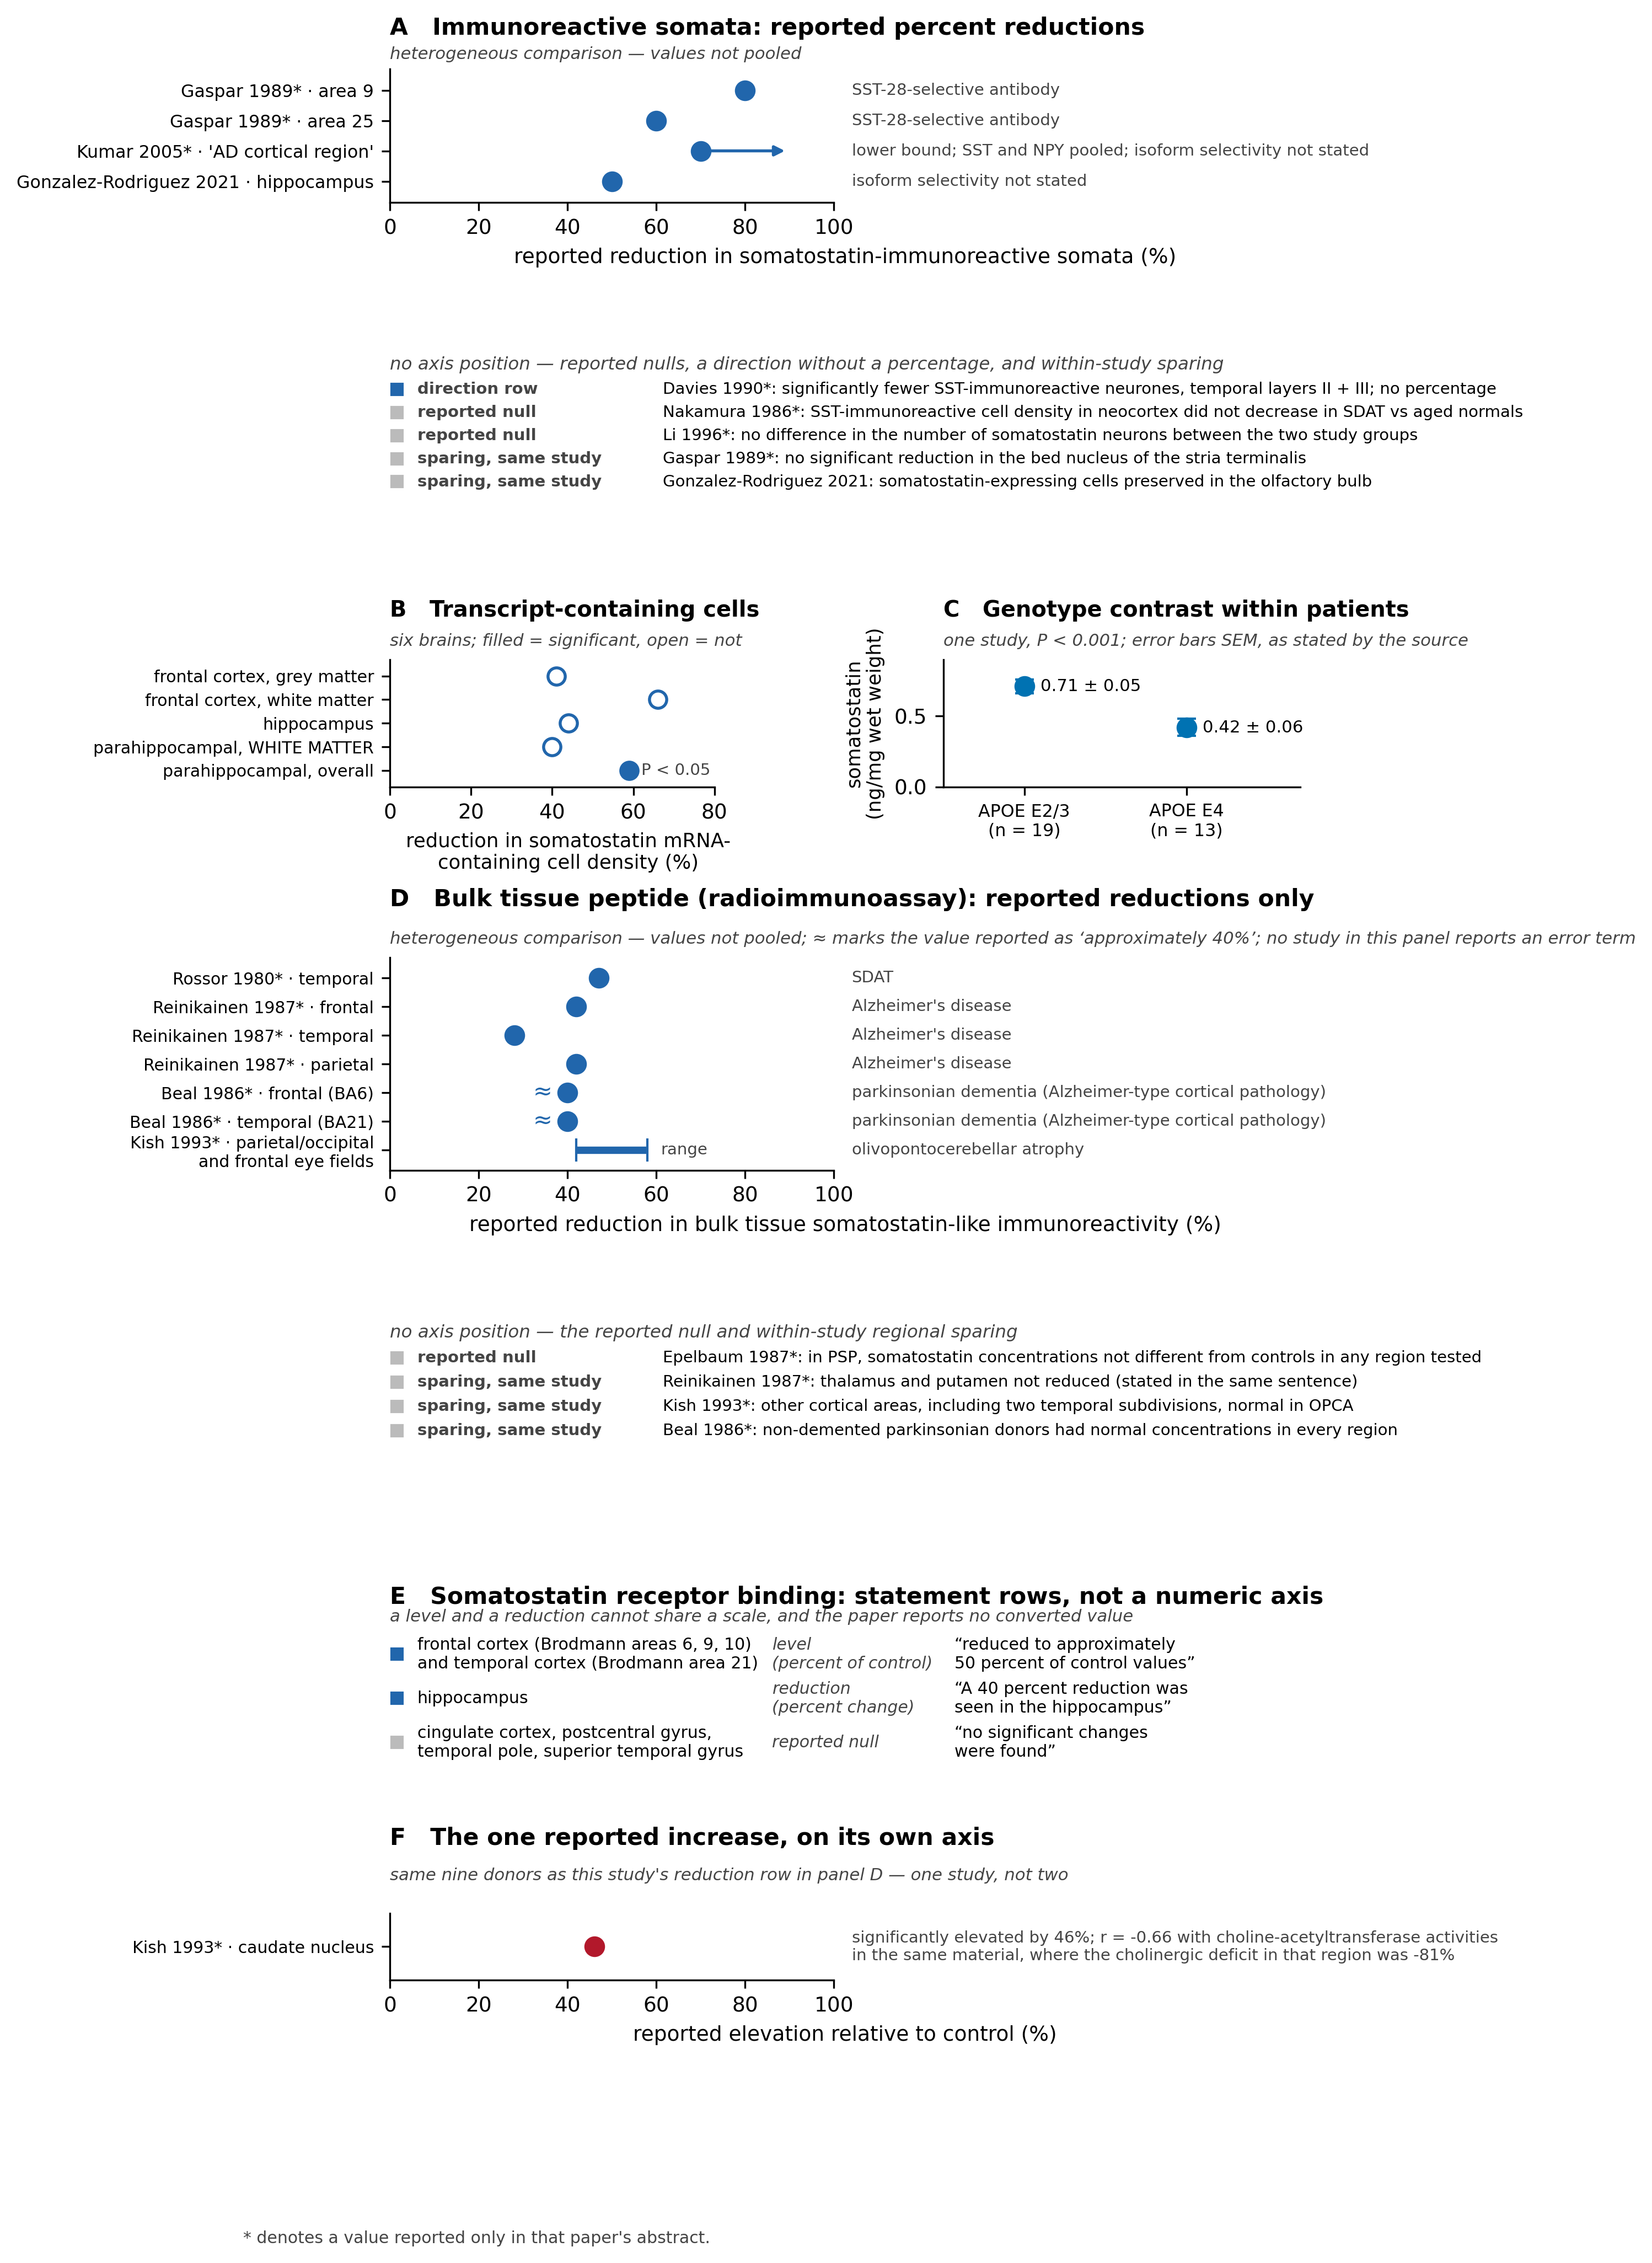
\includegraphics[width=\linewidth]{../figures/fig_sec9_postmortem_somatostatin_deficit_heterogeneity.png}
\caption{\textbf{The human postmortem somatostatin record.} Reported effects are shown by measurand, because the panels are not interchangeable: immunoreactive somata (A), transcript-containing cells (B), bulk peptide concentration (C, D, F) and receptor binding (E) are different quantities. (A) Reported percent reductions in somatostatin-immunoreactive somata only. The antibody target differs between rows: one study counted SST-28-immunoreactive somata with an isoform-selective antibody, and the other count studies report somatostatin immunoreactivity without stating isoform selectivity, so the rows are not the same measurand at antibody level. The -80\% and -60\% values are densities of all SST-28-immunoreactive neurons in cortical areas 9 and 25; that study's conclusion that single, neuropeptide-Y-negative somatostatin neurons in layers II-III and V are preferentially lost is its interpretation of which subpopulation is vulnerable, not the population over which the plotted percentages were computed \citep{Gaspar1989}. The >70\% figure is reported jointly for somatostatin- and neuropeptide-Y-positive neurons and is a lower bound, not a point estimate; it is reported for "AD cortical brain region", so the frontal-cortex label is the study's region of interest and not the region named with that value \citep{Kumar2005}. \citet{Davies1990} reported significantly fewer somatostatin-immunoreactive neurones in layers II + III combined of the temporal cortex and is not a no-effect study for somatic counts; it appears as a direction row because it reports no percentage, its null applies only to fibre length per cortical strip measured by a randomised method, and the same study reports significant reductions in fibre length per cell by a second method. \citet{Nakamura1986} and \citet{Li1996b} report no significant difference in somatostatin-immunoreactive cell number and are shown as named rows off the numeric axis; without them the plotted range is conditioned on having found a quantified reduction. Two of the plotted studies report regions with no loss in the same material - no significant reduction in the bed nucleus of the stria terminalis, and preserved somatostatin-expressing cells in the olfactory bulb while the hippocampus fell by 50\% - and those rows sit beside the affected-region points. Group sizes are reported for only one plotted study (6 SDAT and 5 control cases) and for the direction row (6 control and 6 AD cases); the other two plotted studies report no group size, and no error term is reported anywhere in this panel. (B) All values are from one study of six age- and post mortem delay-matched Alzheimer's disease and control brains; the study's own wording does not state whether six is the number per group or the total, so no per-group size is given, and this is a within-study regional pattern, not a cross-study comparison. Only the parahippocampal reduction (-59\%, P < 0.05) reached significance; the remaining values did not, owing to large between-brain variation. The -59\% and the -40\% are two different parahippocampal measurements - the significant overall parahippocampal reduction and the parahippocampal white-matter value - and must not be read as two regions or averaged; grey and white matter values are plotted separately and must not be averaged. The measurand is the density of somatostatin mRNA-containing cells, and the same study concludes that the ability of cortical cells to express somatostatin messenger RNA is partially preserved \citep{Dournaud1994}. (C) A genotype contrast within patients, not a patient-versus-control disease effect, in a clinically mixed cohort of eleven control subjects, eight borderline patients, six patients with mixed dementia and seven classified as Alzheimer's disease. Values are bulk tissue peptide concentrations in ng/mg wet weight and are not comparable with the cell-count panels; error bars are SEM as stated by the source, and the two genotype strata are n = 19 and n = 13 donors \citep{Grouselle1998}. (D) Every plotted point is bulk tissue somatostatin-like immunoreactivity by radioimmunoassay and cannot separate loss of somatostatin neurons from reduced peptide content per neuron; receptor binding is a different analyte and is in panel E. This axis carries reported reductions only: the one reported increase is in panel F with its own axis, and the progressive supranuclear palsy result is a reported null with no numeric value and no variance, shown as a named row off the numeric axis rather than as a marker at zero \citep{Epelbaum1987}. Entries span four diagnoses (Alzheimer's disease, parkinsonian dementia with Alzheimer-type cortical pathology, olivopontocerebellar atrophy, progressive supranuclear palsy) and each point is labelled with its diagnosis and region. The parkinsonian-dementia value applies only to the demented subgroup with Alzheimer-type cortical pathology; non-demented parkinsonian donors had normal concentrations in every region sampled \citep{Beal1986d}. One value is reported as "approximately 40\%" and one as a 42-58\% range across regions; the qualifier and the range bar are printed and neither is reduced to a point estimate. Regional sparing is as informative as regional loss: thalamus and putamen were not reduced, other cortical areas including two subdivisions of the temporal cortex were normal in olivopontocerebellar atrophy, and in progressive supranuclear palsy concentrations were not different from controls in any region tested. The frontal, temporal and parietal tissue reductions and that study's cerebrospinal fluid result come from different patient sets - histopathologically confirmed cases for tissue, probable Alzheimer's disease for fluid - and are not one cohort sampled twice \citep{Reinikainen1987}. No study in this panel reports an error term; patient-group sizes are 6, 7, 9 and 15 donors. (E) Statement rows, not a numeric axis: the cortical figure is a level (receptor concentration reduced to approximately 50 percent of control) and the hippocampal figure is a reduction (40 percent), they are different quantities, and no conversion between them is performed because the paper reports no converted value. This panel measures somatostatin receptor binding, a different analyte from tissue peptide immunoreactivity, and the same study offers the alternative reading that reduced somatostatin-like immunoreactivity indicates increased release with down-regulation of postsynaptic receptors, so the direction of causation is unresolved. Cingulate cortex, postcentral gyrus, temporal pole and superior temporal gyrus showed no significant change, and no donor count and no error term are reported \citep{Beal1985b}. (F) Somatostatin-like immunoreactivity was significantly elevated by 46\% in the olivopontocerebellar caudate nucleus, the region of that brain with the most severe cholinergic deficit; the value is plotted here, on its own axis, because an increase cannot be placed on the reduction axis of panel D. In the same material the elevation was negatively and significantly correlated with choline-acetyltransferase activities (r = -0.66), and the cholinergic deficit in that region was -81\%. These are the same nine donors as this study's reduction row in panel D, so the two panels report one study, not two. The measurand is bulk tissue somatostatin-like immunoreactivity and the paper itself attributes the change either to abnormal somatostatin metabolism or release or to an increased number of somatostatin-containing neurons, so an increased cell number is not established; no error term is reported \citep{Kish1993}. Study labels marked with an asterisk denote values reported only in that paper's abstract.}
\label{fig-sec9-postmortem-somatostatin-deficit-heterogeneity}
\end{figure}

\begin{figure}[H]
\centering
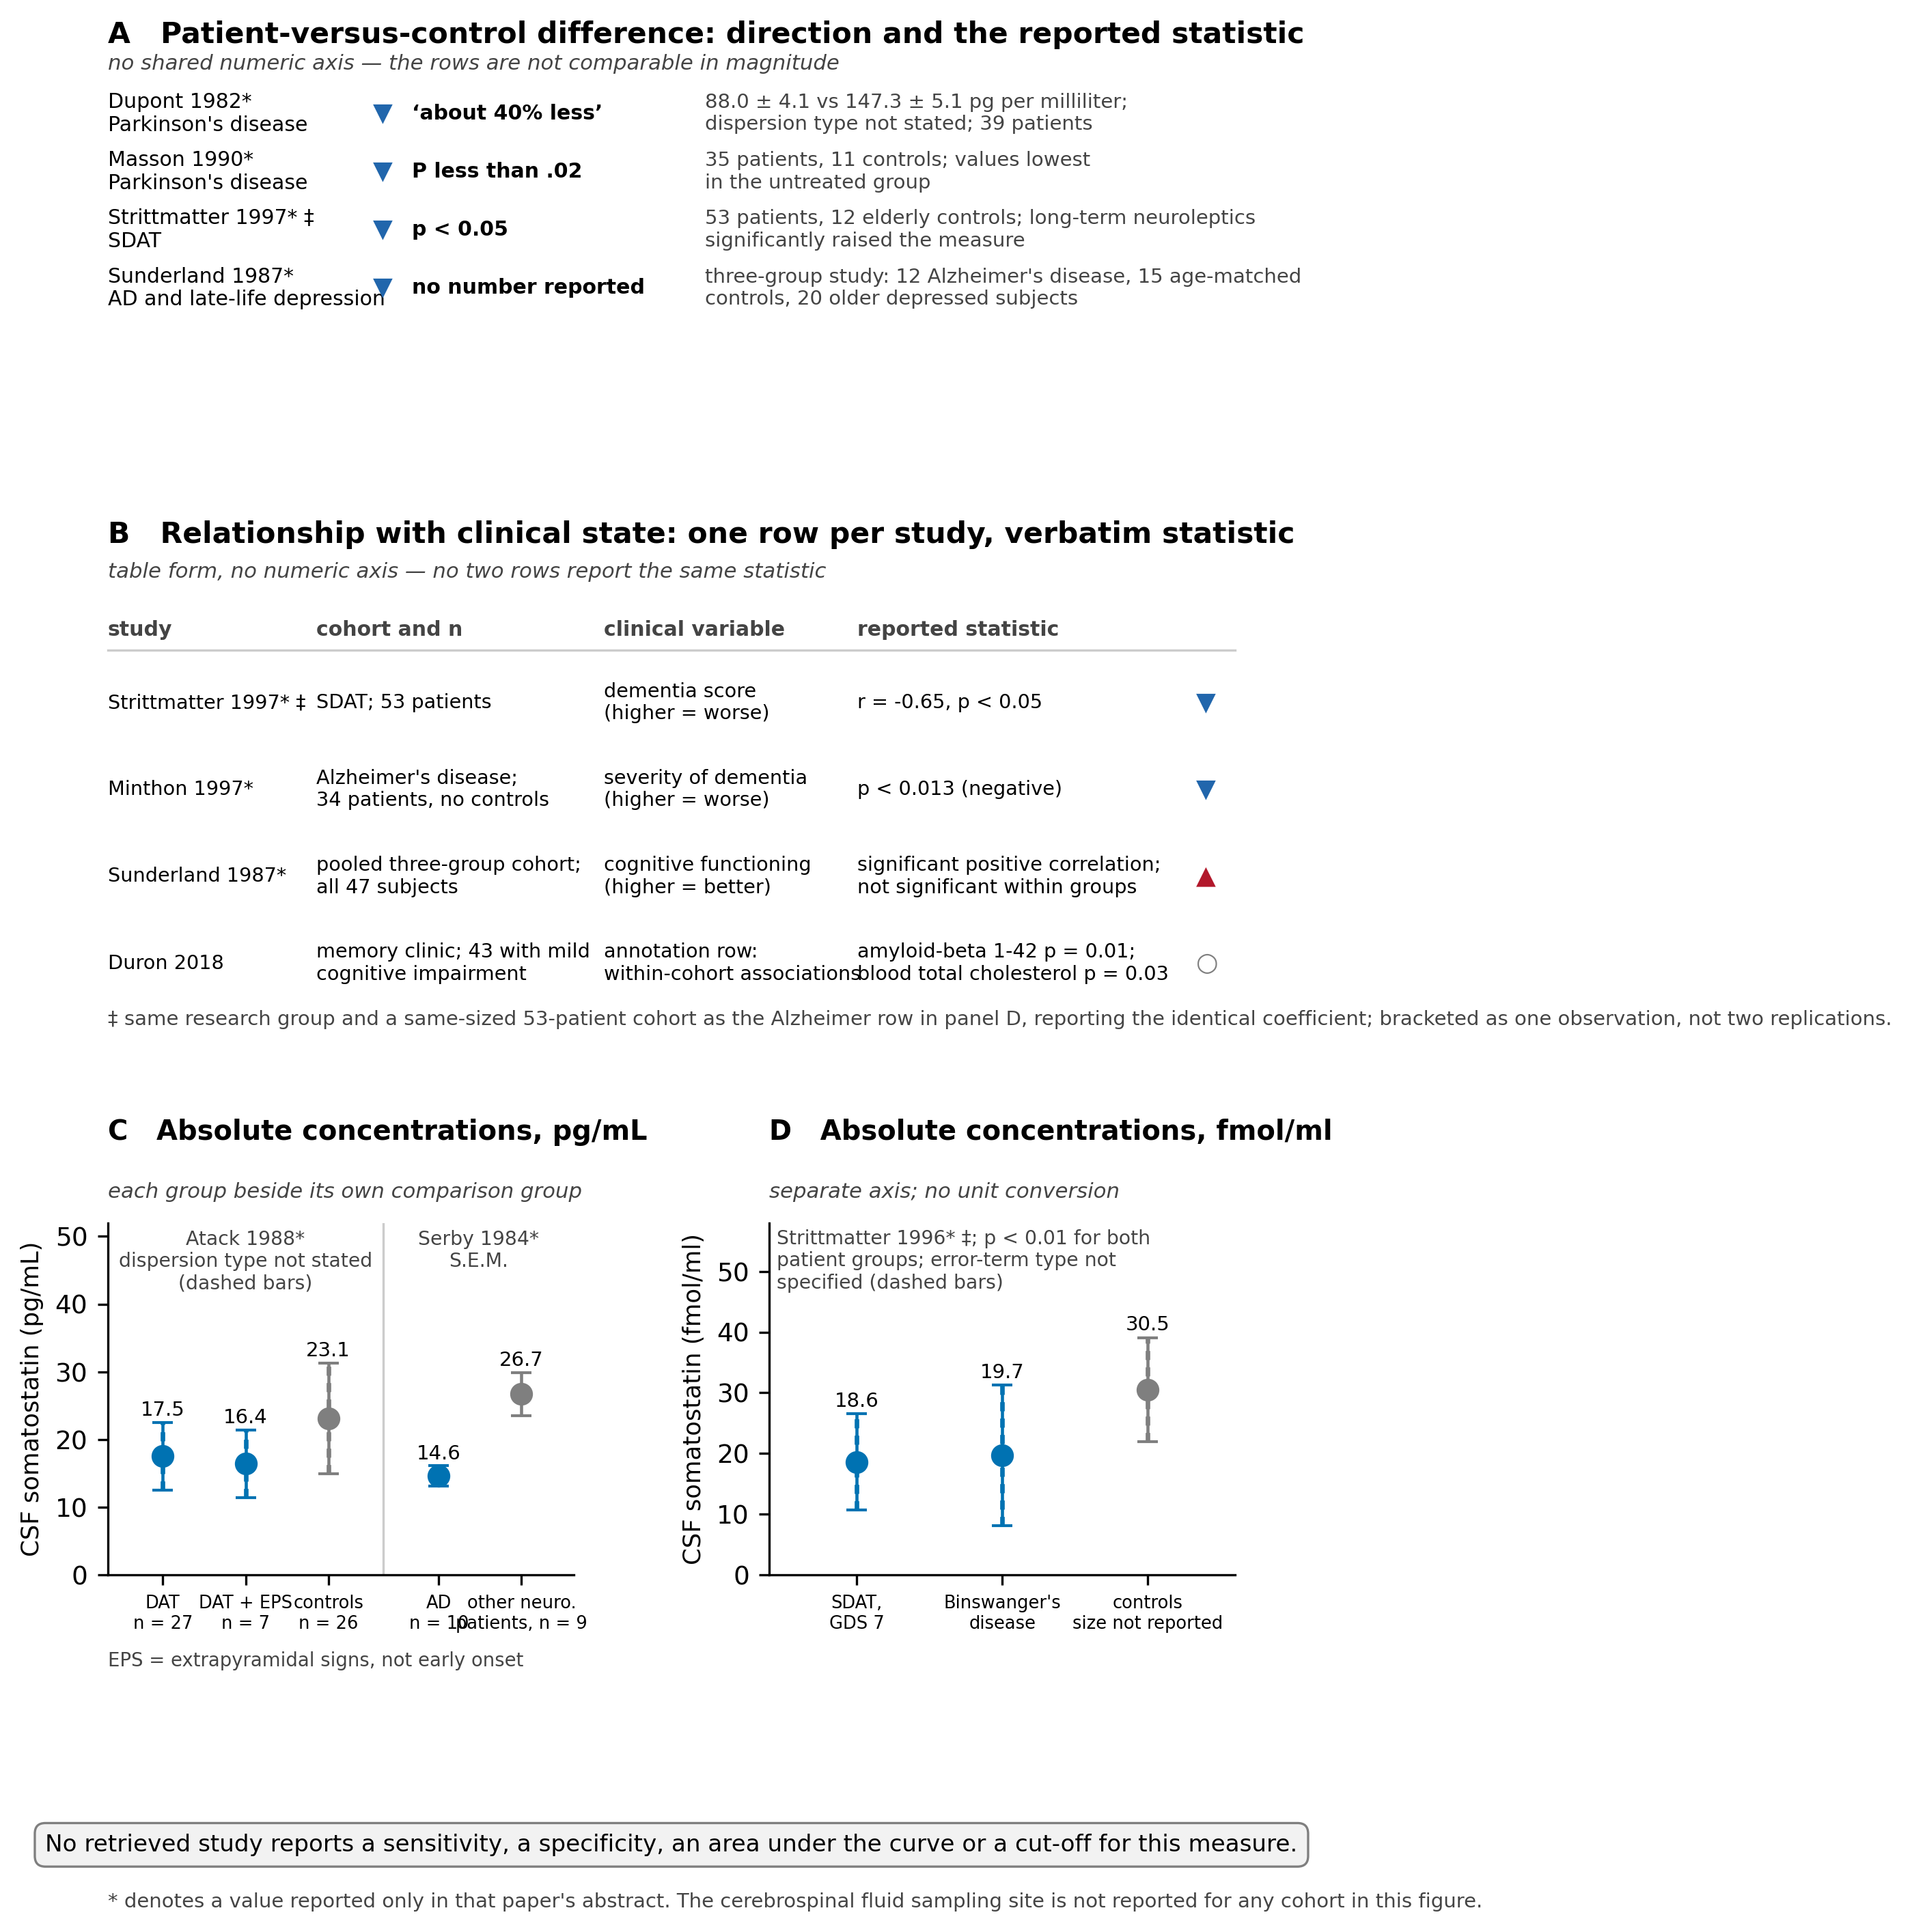
\includegraphics[width=\linewidth]{../figures/fig_sec9_csf_somatostatin_is_not_specific.png}
\caption{\textbf{Cerebrospinal fluid somatostatin across diagnoses.} (A) Rows show direction and the verbatim reported statistic; there is no shared numeric axis and the rows are not comparable in magnitude. Only one study reports absolute concentrations (88.0 +/- 4.1 versus 147.3 +/- 5.1 pg per milliliter), and those +/- values are not identified as standard deviation or standard error; the remaining rows report significance levels or direction only \citep{Dupont1982}. Low cerebrospinal fluid somatostatin is not diagnosis-specific: it is reported in Parkinson's disease, Alzheimer-type dementia and late-life depression alike. Each row rests on a separate radioimmunoassay performed in a different laboratory and no cross-calibration between them is reported, so the rows carry no common concentration scale; only one study in this section states its assay's cross-reactivity with cortistatin-like immunoreactivity, and it is on a different figure. Medication is uncontrolled: values were lowest in untreated Parkinson's disease patients \citep{Masson1990}, and long-term neuroleptics significantly raised the measure in one Alzheimer-type cohort \citep{Strittmatter1997}. The dementia-and-depression row reports no number: what is reported is that patients with dementia or depression had lower concentrations than control subjects; it comes from a three-group study (12 Alzheimer's disease, 15 age-matched controls, 20 older depressed subjects) and its direction statement covers both patient groups, not the 12 Alzheimer donors alone \citep{Sunderland1987}. One Alzheimer-type row comes from the same research group and a same-sized 53-patient cohort as the Binswanger comparison in panel D, reporting the identical coefficient, and the two are bracketed rather than counted as independent observations. (B) Table form, no numeric axis: no two rows report the same statistic, so coefficients, significance levels and direction statements are quoted verbatim and are not comparable in magnitude. Correlation signs differ because the clinical variable differs - somatostatin falls with greater dementia severity and rises with better cognitive function - and both indicate the same direction of effect; the cognitive-functioning correlation is reported across all 47 subjects of its three-group study, not across the 12 Alzheimer donors listed in the n column \citep{Sunderland1987}. One cohort includes no control subjects, so its severity correlation says nothing about absolute reduction \citep{Minthon1997}. The memory-clinic row reports within-cohort biomarker associations (amyloid-beta 1-42, total cholesterol), not a relationship with cognition or a patient-versus-control difference, and is an annotation row \citep{Duron2018}. (C) Absolute concentrations in pg/mL, each patient group drawn beside its own comparison group. The second Alzheimer-type group is dementia of the Alzheimer type with extrapyramidal signs (seven donors), not early-onset disease \citep{Atack1988}. Error bars are not uniform: one study's +/- values are not identified as standard deviation or standard error and are labelled unspecified, while the other states S.E.M. \citep{Serby1984}. One study's comparison group is 9 patients with other neurological conditions, not healthy controls. Neither study states the calibration status or the provenance of its radioimmunoassay; they are separate assays with no cross-calibration reported between them. In one study the concentrations were unrelated to dementia severity and did not change during disease progression. (D) Values in fmol/ml on their own axis, not interconvertible with panel C because the assay measures a mixture of somatostatin molecular forms, so no single molecular weight applies. The Alzheimer value applies only to patients at the most severe dementia stage (GDS 7), whereas the pg/mL studies pool all severities and one of them found concentrations unrelated to severity; the second patient group is Binswanger's disease, a subcortical vascular dementia, not a primary neurodegenerative dementia. The reported error terms are not identified as standard deviation or standard error, the study states neither the calibration status nor the provenance of its radioimmunoassay, and this Alzheimer-type group is the one bracketed with panel A - same research group, same-sized 53-patient cohort - rather than an independent observation \citep{Strittmatter1996b}. The cerebrospinal fluid sampling site is not reported for any cohort in this figure. No retrieved study reports a sensitivity, specificity, area under the curve or cut-off for this measure.}
\label{fig-sec9-csf-somatostatin-is-not-specific}
\end{figure}

\begin{figure}[H]
\centering
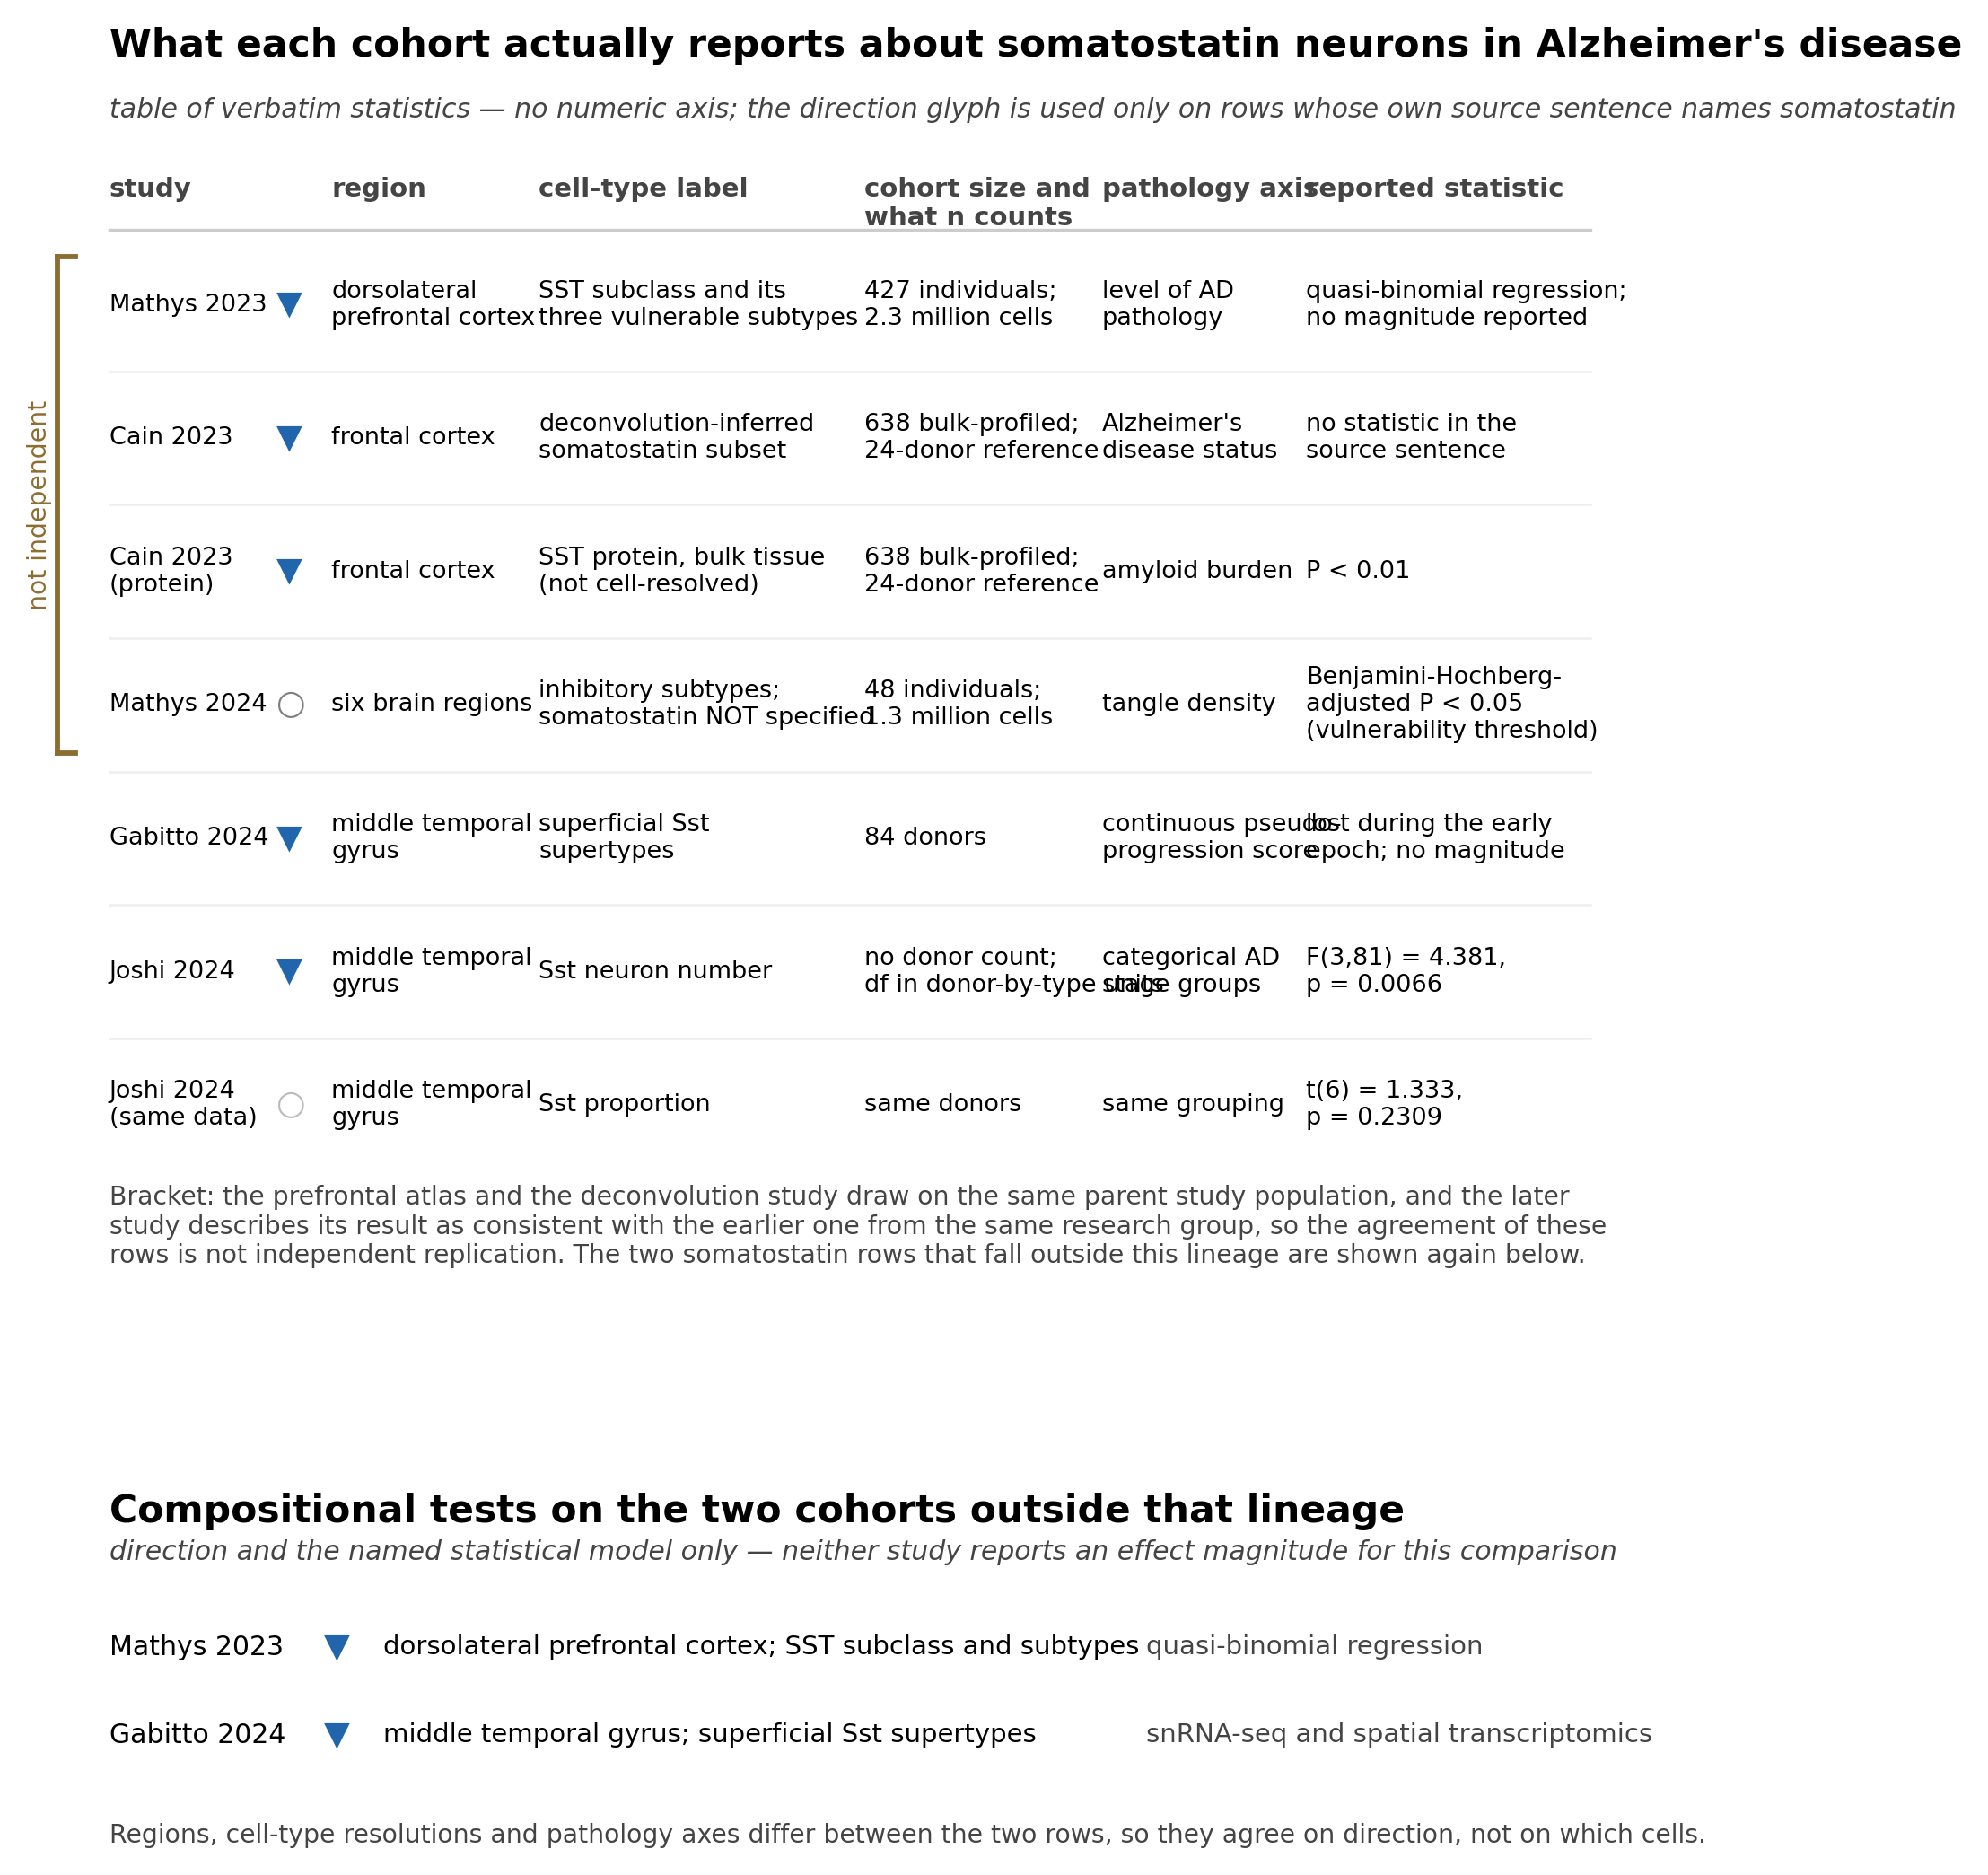
\includegraphics[width=\linewidth]{../figures/fig_sec9_single_nucleus_cohort_convergence.png}
\caption{\textbf{Single-nucleus and deconvolution evidence for somatostatin neuron depletion in Alzheimer's disease.} Upper panel: one row per study-observable, with no numeric axis anywhere, because no two rows report the same quantity; direction of effect and the verbatim reported statistic are shown, not comparable magnitudes. Cell-type labels are not matched across studies - subclass, supertype, high-resolution type and deconvolution-inferred subset denote different entities. Three rows are linked by a bracket that rests on the later study describing its result as consistent with the earlier one and on those two studies sharing a research group; the prefrontal atlas and the deconvolution study draw on the same parent study population, so their agreement is not independent replication \citep{Mathys2023,Cain2023,Mathys2024}. The multiregion atlas row identifies vulnerable inhibitory subtypes without specifying somatostatin and therefore carries a neutral open marker rather than the depletion glyph; its Benjamini-Hochberg-adjusted P < 0.05 is the threshold for classification as vulnerable, set by that study's own definition of a vulnerable subtype \citep{Mathys2024}. The deconvolution study's reported P < 0.01 is for somatostatin protein against amyloid burden, not for a counted cell population, and its inferred cell subset is a separate row with no statistic \citep{Cain2023}. Pathology axes differ (level of Alzheimer pathology, a continuous pseudo-progression score, tangle density, amyloid burden, categorical stage), so "depleted in Alzheimer's disease" is anchored to a different variable in each row. The stage-grouped study reports a significant group difference in Sst neuron number and a null proportion test from the same dataset; both are shown as adjacent rows, each printing its own verbatim statistic \citep{Joshi2024}. Sample sizes count incompatible units across rows - donors profiled by single-nucleus sequencing, individuals profiled in bulk with proportions inferred from a separate 24-donor reference, and donor-by-type units - and are printed as text rather than encoded graphically; one row carries no donor count at all. Each row names its region; the region named for the pseudo-progression study is the middle temporal gyrus, the only region that study reports for this measurement \citep{Gabitto2024}. Lower panel: the two cohorts that apply a compositional test to somatostatin neurons at subclass or supertype level outside a shared lineage, shown as direction and the named statistical model only, since neither study reports an effect magnitude for this comparison. Their regions and cell-type resolutions differ (subclass in dorsolateral prefrontal cortex versus superficial supertypes in the middle temporal gyrus) and their pathology axes differ (level of Alzheimer pathology versus a continuous quantitative-neuropathology pseudo-progression score), so the rows agree on direction, not on which cells.}
\label{fig-sec9-single-nucleus-cohort-convergence}
\end{figure}

\section{Therapeutic Strategies: Somatostatin Receptor Agonists, Interneuron-Targeted Interventions, and Neuromodulation}
\label{sec-therapeutics}

Where \ref{sec-human-evidence} left the somatostatin deficit established in human cortex but unaccompanied by any fluid measure that could grade it, therapy supplies the direct test: if the deficit is causal, correcting it should change the disease. No study retrieved by these searches has run that test on the SST class. The interventions assembled below are the closest approaches to it --- receptor agonism, replacement of the cells, gene therapy addressed to inhibitory neurons, excitability-lowering drugs, and stimulation of the circuits those cells inhabit --- and each of them either engages a different cell class, stops short of a disease model, or stops short of a controlled clinical endpoint. The pattern that organises the section is not disease biology but study design: across these literatures the reported magnitude of benefit falls as the design that produced it becomes more rigorous.

\subsection{Somatostatin receptor agonists: a clean rodent pathway and an unclosed translational chain}
\label{sec-10-sstr-agonists}

The most coherent pharmacological case for acting on the somatostatin axis comes from a single series of studies of the SSTR4-selective agonist NNC 26-9100, and its coherence is also its limitation. Delivered intracerebroventricularly at 0.2 $\mu$g in SAMP8 mice, the compound produced what its authors describe as an approximately 2-fold enhancement in recognition memory (P < 0.01) \citep{Sandoval2012}; given chronically by the intraperitoneal route at 20 $\mu$g it lowered brain amyloid-$\beta$ (A$\beta$) x-42, though the report gives a direction and P < 0.05 rather than a magnitude \citep{Sandoval2011}; co-administration of the metalloproteinase inhibitor phosphoramidon at 10 mM left A$\beta$ x-42 at levels the source describes as identical to vehicle and higher than with the agonist alone (P < 0.01 against agonist alone; no test is reported for the identity with vehicle), placing neprilysin causally downstream of the receptor \citep{Sandoval2013}; and transcriptional profiling in 3xTg-AD mice found subcortical increases in \emph{Nep1} (2.4-fold), \emph{Ide} (4.4-fold) and \emph{Sst} (4.4-fold) at 24 h that were not statistically significant \citep{Sandoval2019}. Medicinal chemistry has continued to produce SSTR4-selective chemical series with Alzheimer's disease named as an intended indication \citep{AbdelMagid2024}, and structural work on the receptor family places subtype discrimination largely in extracellular loop 2, consistent with the earlier mutagenesis that work reviews rather than repeats --- a loop swap reported to reduce octreotide binding by \textasciitilde{}40-fold, and a position-7 phenylalanine substitution reported to raise SSTR2 affinity \textasciitilde{}6-fold with little effect on SSTR4 \citep{Zhao2022}. Two limits bound the whole programme. All four efficacy entries test one compound from one closely related research programme, so their agreement is convergence within a programme and not independent replication; and the doses are not interchangeable, because 0.2 $\mu$g into the ventricle and 20 $\mu$g into the peritoneum are the blood--brain barrier problem written as a dose. No replicating study for the phosphoramidon result was retrieved by these searches, more than a decade after publication. It also establishes less than it is usually asked to: blocking the enzyme abolishes the amyloid effect, which shows the effect requires neprilysin activity, but no study directly measuring a rise in brain neprilysin activity under pharmacological SSTR agonism was retrieved by these searches, so the step most often quoted as the mechanism is inferred rather than observed.

\ref{fig-sec10-sstr4-agonist-dose-route-mechanism} tabulates the four results rather than plotting them, because they do not share a measurement scale.

\begin{figure}[H]
\centering
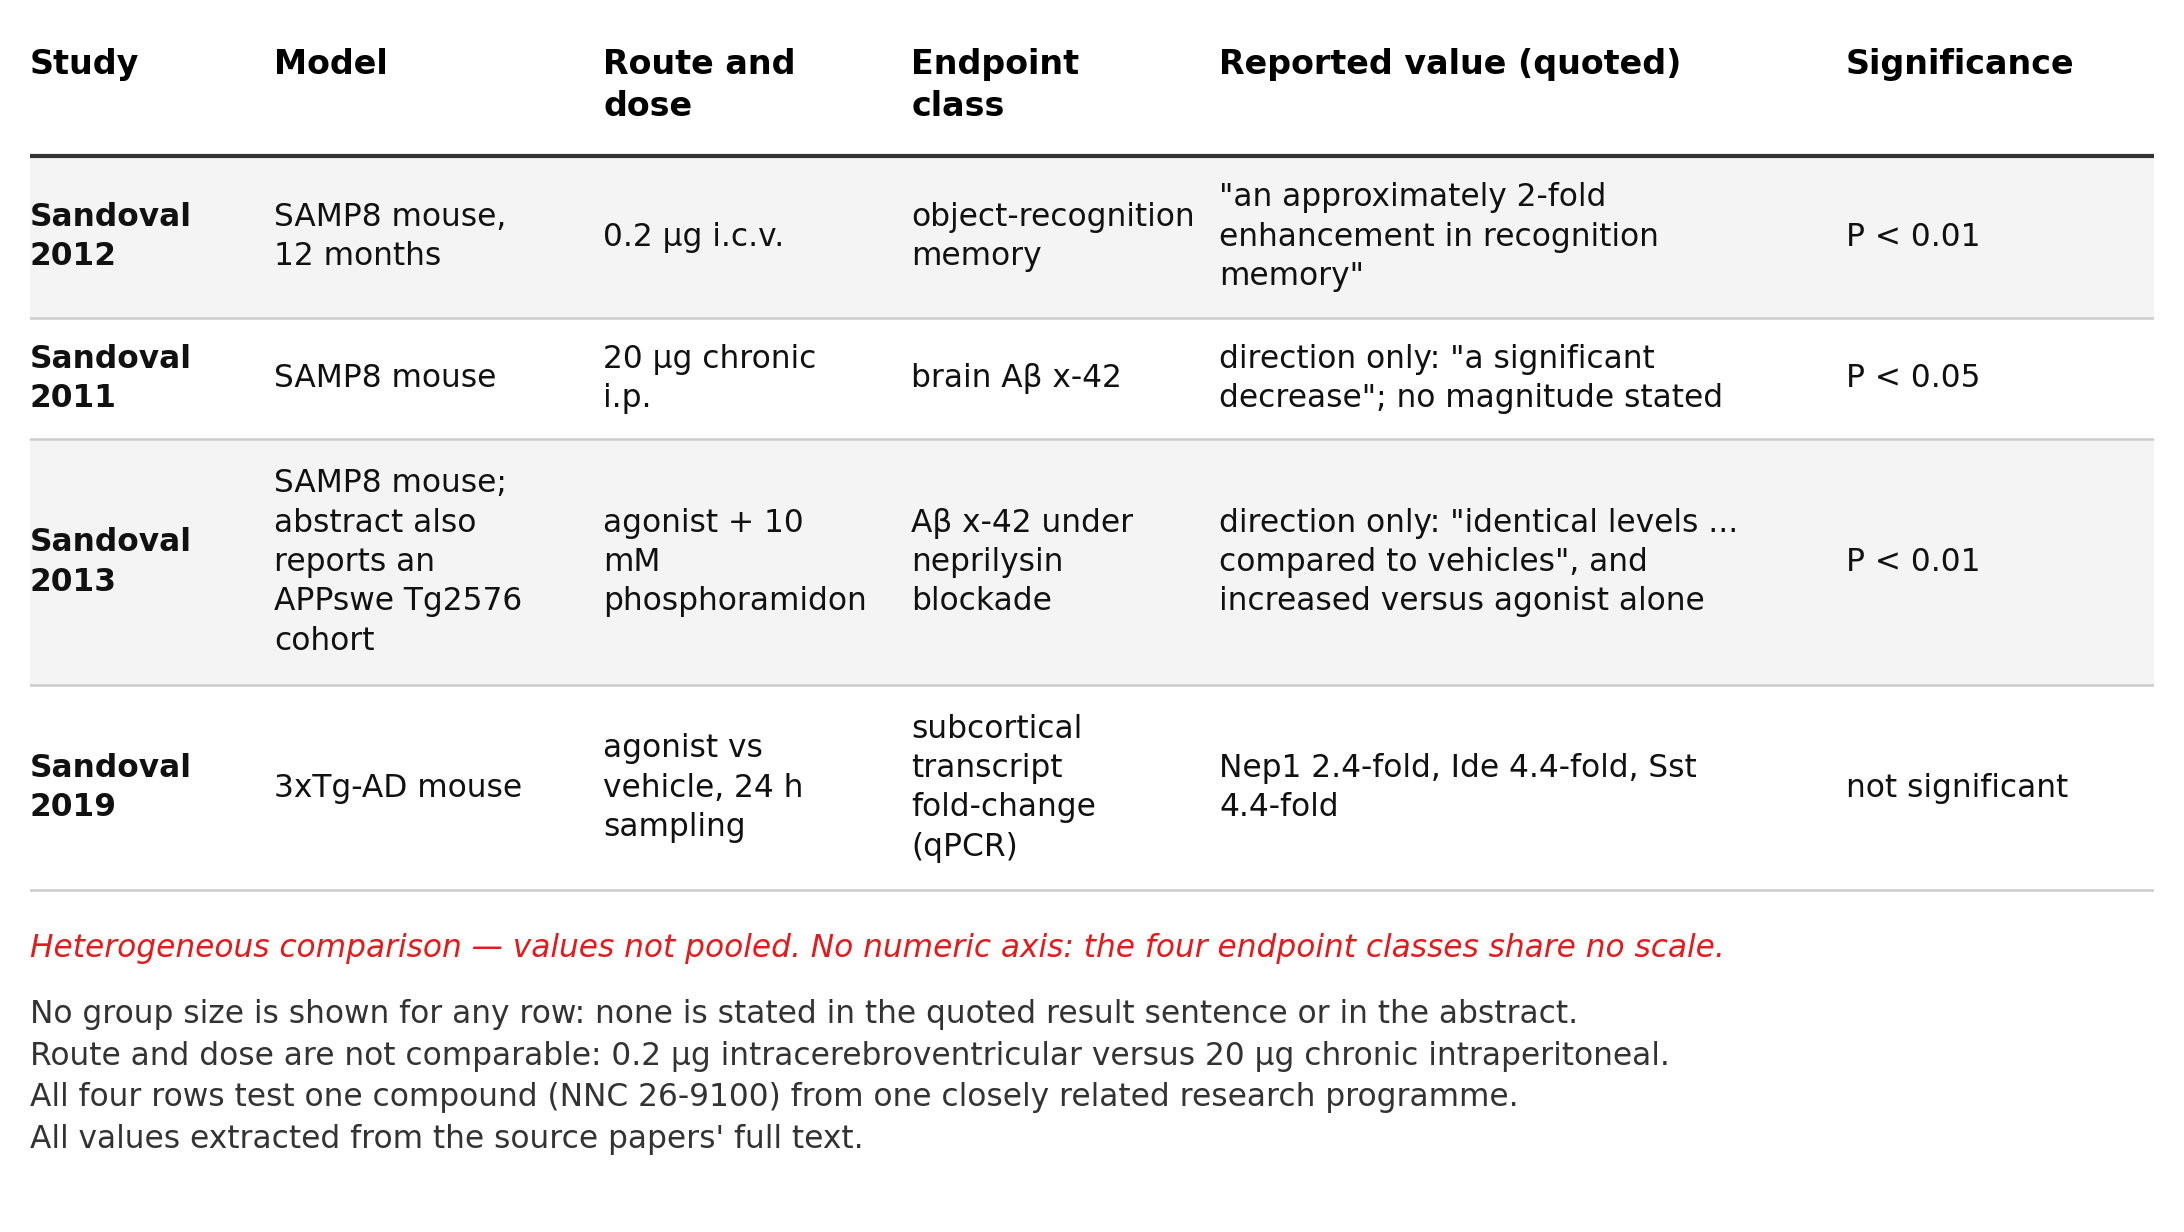
\includegraphics[width=\linewidth]{../figures/fig_sec10_sstr4_agonist_dose_route_mechanism.png}
\caption{\textbf{SSTR4 agonist: dose, route and endpoint.} Four reported results for the SSTR4-selective agonist NNC 26-9100, tabulated with their quoted values \citep{Sandoval2012,Sandoval2011,Sandoval2013,Sandoval2019}. No shared numeric axis: the four results are a behavioural preference ratio, two A$\beta$ x-42 protein measurements and a set of qPCR fold-changes. Route and dose differ: 0.2 $\mu$g intracerebroventricular versus 20 $\mu$g chronic intraperitoneal; the doses are not comparable. Two entries report only a direction of effect and a p value; no magnitude is shown for them. The Sandoval 2012 row quotes the published wording, "an approximately 2-fold enhancement in recognition memory". Sandoval 2019 was performed in 3xTg-AD mice, not SAMP8; the fold-changes shown are the non-significant subcortical values at 24 h ("no statistically significant differences were found between NNC 26-9100 and vehicle treatment"), and the same study's cortical counterparts at 24 h were larger, the abstract reporting the failure to reach statistical significance only for the subcortical tissue. No group size is shown for any row: none of the four reports states one in its abstract or in the sentence reporting the result. All entries test one compound from one research programme; this is convergence within a programme, not independent replication.}
\label{fig-sec10-sstr4-agonist-dose-route-mechanism}
\end{figure}

The clinically available short analogues cannot test this pathway. The octapeptide and hexapeptide analogues, which are the class the receptor-pharmacology record describes, bind well to only three of the five receptors --- SSTR2, SSTR3 and SSTR5 --- and therefore cannot engage the subtype the amyloid-clearance argument depends on \citep{Patel1999}, while their formulation constraints are those of peptides: food reduces absorption of oral octreotide by about 90\% \citep{Periferakis2024}. Systemic octreotide nonetheless produces central effects in a rat model of post-traumatic stress, attenuating HPA-axis hyperactivity, neuroinflammation and oxidative stress, with the authors themselves noting that direct receptor-mediated mechanisms remain unconfirmed \citep{Motamedy2026}. Related peptides of the same family act on tissue compartments that drug delivery must cross: loss of cortistatin dysregulates 613 genes in brain endothelium \citep{CastilloGonzalez2023}, cortistatin supplementation shifts neuronal mitochondrial networks toward a tubular morphology (to 84\% in wild-type and 40\% in mutant neurons) \citep{GonzalezGarcia2026}, and systemic cortistatin restores pole-test performance in MPTP-intoxicated mice \citep{SerranoMartinez2024}. Barrier-opening technologies are advancing in parallel --- focused ultrasound with microbubbles is reported practical, reversible and generally safe in selected Alzheimer's cohorts, though without conclusive evidence linking the opening to clinical benefit \citep{Desale2026}, and ultrasound-assisted lipid nanoparticle delivery achieved gene editing comparable to the same group's earlier ultrasound-delivered viral system while raising the astrocyte-targeted expression fraction above that group's previously reported 12.9\%, in a comparison against a published number rather than a controlled head-to-head, and in astrocytes rather than any interneuron population \citep{Zheng2026}. Two absences matter more than any of this: no clinical trial of an SSTR-selective agonist in any neurodegenerative indication was retrieved by these searches, and no quantitative human CNS exposure data for the octreotide class surfaced, so proposals to repurpose existing analogues remain unanchored. The receptor pharmacology that would make such a trial interpretable is set out in \ref{sec-sst-identity}.

\subsection{Raising neprilysin: downstream effector, or the wrong amyloid pool}
\label{sec-10-neprilysin}

The SSTR4 chain terminates in neprilysin, and the independent literature on raising neprilysin directly shows why terminating there is not the same as succeeding. Vector-delivered neprilysin is axonally transported to presynaptic terminals and abolished the rise in A$\beta$ in the hippocampal formation of neprilysin-deficient mice, with reductions appearing contralateral to the injection \citep{Iwata2004}. Against that, a synthesis of hAPP/NEP double-transgenic data reports that a 50\% fall in soluble A$\beta$ with prevention of plaque formation left oligomer reduction undemonstrated and behavioural outcome unassessed, attributing the dissociation to neprilysin's inability to cleave some naturally occurring oligomeric A$\beta$ species \citep{Grimm2013}. A review of neprilysin biology notes that the enzyme is promiscuous, metabolising enkephalins, substance P and bradykinin alongside A$\beta$, so raising its activity would not be a clean intervention \citep{Saxena2024}; no primary measurement of off-target neuropeptide consequences under a neprilysin-raising therapy was retrieved by these searches. The human anchor for the whole chain remains correlational, and narrower than the chain it supports: somatostatin content is reduced by approximately 50\% in the anterior olfactory nucleus in Alzheimer's disease, with most remaining somatostatin-expressing elements co-localising with A$\beta$ (65.43\%) \citep{SaizSanchez2010} --- one region, recorded at abstract level. The upstream step --- that loss of somatostatin signalling is what lowers neprilysin in human disease --- is contested where it is examined at all, and is treated in \ref{sec-alzheimers}; its primary demonstration in human tissue was not retrieved here, which makes the therapeutic prior for SSTR agonism weaker than its frequent restatement in reviews implies.

\begin{quote}
\noindent\textbf{Evidence Conflict}\par
\textbf{Which amyloid pool is therapeutically decisive for neprilysin-raising strategies?} Vector-delivered neprilysin abolishes the A$\beta$ increase in neprilysin-deficient hippocampus and reduces it in young mutant APP mice \citep{Iwata2004}, whereas the synthesis of hAPP/NEP double-transgenic data reports a 50\% soluble-A$\beta$ reduction and plaque prevention without a demonstrated fall in oligomers, on the stated grounds that neprilysin cannot cleave some naturally occurring oligomeric species \citep{Grimm2013}. The disagreement is not about whether neprilysin degrades A$\beta$ but about which pool matters; the two sides measure different pools, and the question is unresolved.

\end{quote}

\subsection{Gamma entrainment: what is stimulated, and what shrinks as rigor rises}
\label{sec-10-gamma}

Gamma sensory stimulation is the most publicised interneuron-targeted strategy in this field and the one whose mechanistic premise is least secure. Three claims must be separated: that 40 Hz stimulation entrains the endogenous oscillator, that it lowers amyloid, and that it improves cognition. The frequency choice has a biophysical rationale --- human steady-state visual evoked potentials show resonance peaks near 10, 20, 40 and 80 Hz \citep{Herrmann2001} --- and the paradigm's originating report measured soluble amyloid one hour after a single hour of flicker, finding A$\beta$1-40 reduced by 57.96\% and A$\beta$1-42 by 57.97\% in visual cortex relative to dark controls \citep{Iaccarino2016}. Direct multisite silicon-probe recording in APP/PS1 and 5xFAD mice, however, found that 40 Hz flicker did not engage native gamma oscillations in visual cortex, entorhinal cortex or hippocampus, with weak hippocampal spike responses \citep{Soula2023}; no independent confirmation that 40 Hz sensory stimulation entrains native gamma in deep structures was retrieved by these searches. The amyloid endpoint, meanwhile, is intensity-dependent: in 3xTg-AD mice A$\beta$ burden fell under high-intensity (1100--1500 lux) but not low-intensity (100--500 lux) 40 Hz stimulation \citep{Gu2026}, an exposure variable that is unreported in much of the downstream work. The amyloid endpoint does replicate across sensory modality: four weeks of 40 Hz vibrotactile stimulation lowered cortical soluble A$\beta$40 and A$\beta$42 and hippocampal plaque burden \citep{Nam2026}, as the intensity-controlled study does at high illumination \citep{Gu2026}; both name the originating report among the work they replicate \citep{Iaccarino2016}. Two further results are often enrolled in the same argument but measure something else. Intraoperative 40 Hz flicker preserved novel-object recognition memory after anaesthesia and surgery \citep{Jiang2026}, an endpoint that is behavioural rather than molecular and a model that is perioperative rather than neurodegenerative, and the record for it is contested rather than replicated. The frequency control --- 22 days of 80 Hz stimulation leaving V1 neuronal loss in P301S tau mice unchanged \citep{Adaikkan2019} --- was run on neuronal loss in a tauopathy, not on amyloid, and carries no replication here. Where optogenetic drive is reported to have restored gamma and spatial memory in amyloid models, the targeted cells were medial septal parvalbumin neurons, not SST cells --- a result known here only through a survey of this literature, which attributes it to an earlier experiment whose primary report was not retrieved by these searches \citep{Zhang2024a}. That is the central qualification for this review: the entrainment literature is built on fast-spiking parvalbumin circuitry, and no study retrieved here selectively drove SST interneurons in a neurodegeneration model and measured amyloid, tau or cognition. Whether 40 Hz stimulation engages the endogenous oscillator at all is examined in \ref{sec-circuit-consequences}.

\begin{quote}
\noindent\textbf{Evidence Conflict}\par
\textbf{Does 40 Hz flicker entrain native gamma, and does the amyloid effect generalise or translate?} Three recorded disagreements share one party: the originating report, which attributes a large reduction of soluble A$\beta$1-40 and A$\beta$1-42 in visual cortex to one hour of 40 Hz flicker \citep{Iaccarino2016}. On mechanism, multisite silicon-probe recording in two amyloid models finds no engagement of native gamma in visual cortex, entorhinal cortex or hippocampus \citep{Soula2023}, so the process the originating study proposes \citep{Iaccarino2016} is not observed where it is looked for directly; the axis is recording method and the level at which entrainment is defined, and the disagreement is unresolved. On dose, an intensity-controlled study lowers A$\beta$ burden only at high illumination \citep{Gu2026}, which bounds rather than overturns the original \citep{Iaccarino2016} and is partially resolved in favour of a threshold --- stimulus intensity being an axis left unreported in much of the downstream literature. On translation, the individual trials tabulated in a synthesis of clinical gamma stimulation report no significant change in overall cognition tests under protocols of up to four weeks, although that synthesis also tabulates longer protocols with reported cognitive improvement and its authors' own conclusion is favourable to the technique \citep{DePaolis2024}, which disagrees with the mouse molecular result \citep{Iaccarino2016} along species and endpoint --- amyloid load in mouse cortex against global cognition in patients, with delivery modality differing as well --- and is also open.

\end{quote}

In patients, the effect sizes order themselves by design. A random-effects meta-analysis of randomized 40 Hz light stimulation trials --- eleven studies, 341 participants --- found no significant cognitive difference from control (standardised mean difference, SMD = 0.16, 95\% CI $-$0.36 to 0.68, P = 0.55) alongside a significant difference in structural brain measures, and no significant increase in overall adverse events, although the risk of tinnitus was significantly raised \citep{Ang2025}. A single session in 62 healthy adults improved psychomotor vigilance accuracy (Kruskal--Wallis $\chi$$^{2}$(2) = 7.98, p = 0.018) \citep{Attokaren2026}, and a randomized sham-controlled trial of transcranial and intranasal photobiomodulation in post-COVID cognitive impairment --- a near-infrared photobiomodulation trial rather than sensory gamma entrainment, its source stating no pulse rate --- reported a significant difference of 0.059 (95\% CI 0.007--0.111, p = 0.028, Cohen's d $\approx$ 0.44) in a prespecified exploratory subgroup under 45 years, while its primary outcome, 0.043 (95\% CI $-$0.007 to 0.092), was not significant at p = 0.088 \citep{Lim2026}. Feasibility and open-label work supplies the rest of the ladder: entrainment does not accumulate with chronic exposure, the number of entrained EEG channels being unchanged before versus after flicker exposure (all P > 0.11) \citep{He2021}; a sham-controlled trial reported maintained daily-living function against a declining sham arm of eight participants \citep{Cimenser2021}; long-term follow-up diverged by onset subtype, with the 40 Hz EEG response declining in early-onset and increasing in late-onset patients, who improved on MMSE, CDR and FAS against matched registry comparators \citep{Chan2025}; and a single open-label record whose reported outcome could not be attributed to the work cited for it \citep{Yamada2026} cannot be placed on the ladder at all. \ref{fig-sec10-gamma-stimulation-evidence-ladder} sets these human results beside one another, each on the scale its own source reports. The two best-controlled results disagree outright, and ranking them does not settle it: population, outcome measure and exposure duration all differ between the pooled patient trials \citep{Ang2025} and the single-session study in healthy adults \citep{Attokaren2026}, so neither excludes the other and whether 40 Hz sensory stimulation produces measurable cognitive benefit remains open. New trials continue to register, extending the paradigm to post-illness cognitive impairment \citep{Fu2026} and to home-based personalised transcranial alternating current stimulation (tACS) with an enrolment target of 40 participants \citep{Brechet2026}. The strongest human claim is structural rather than cognitive: over six months of daily audiovisual stimulation, total cerebral white matter volume rose by 0.17 $\pm$ 1.08\% in the active arm while falling by 2.54 $\pm$ 1.38\% under sham (p < 0.038) \citep{Da2024a}, and corpus callosum area changed by 0.20 $\pm$ 0.70\% versus $-$2.08 $\pm$ 0.87\% \citep{Da2024b}. Both are analyses of one randomized cohort from a single device programme with overlapping, unequal subsets, which is the weakest form of convergence this review encounters, and no independent group's structural replication was retrieved.

\begin{figure}[H]
\centering
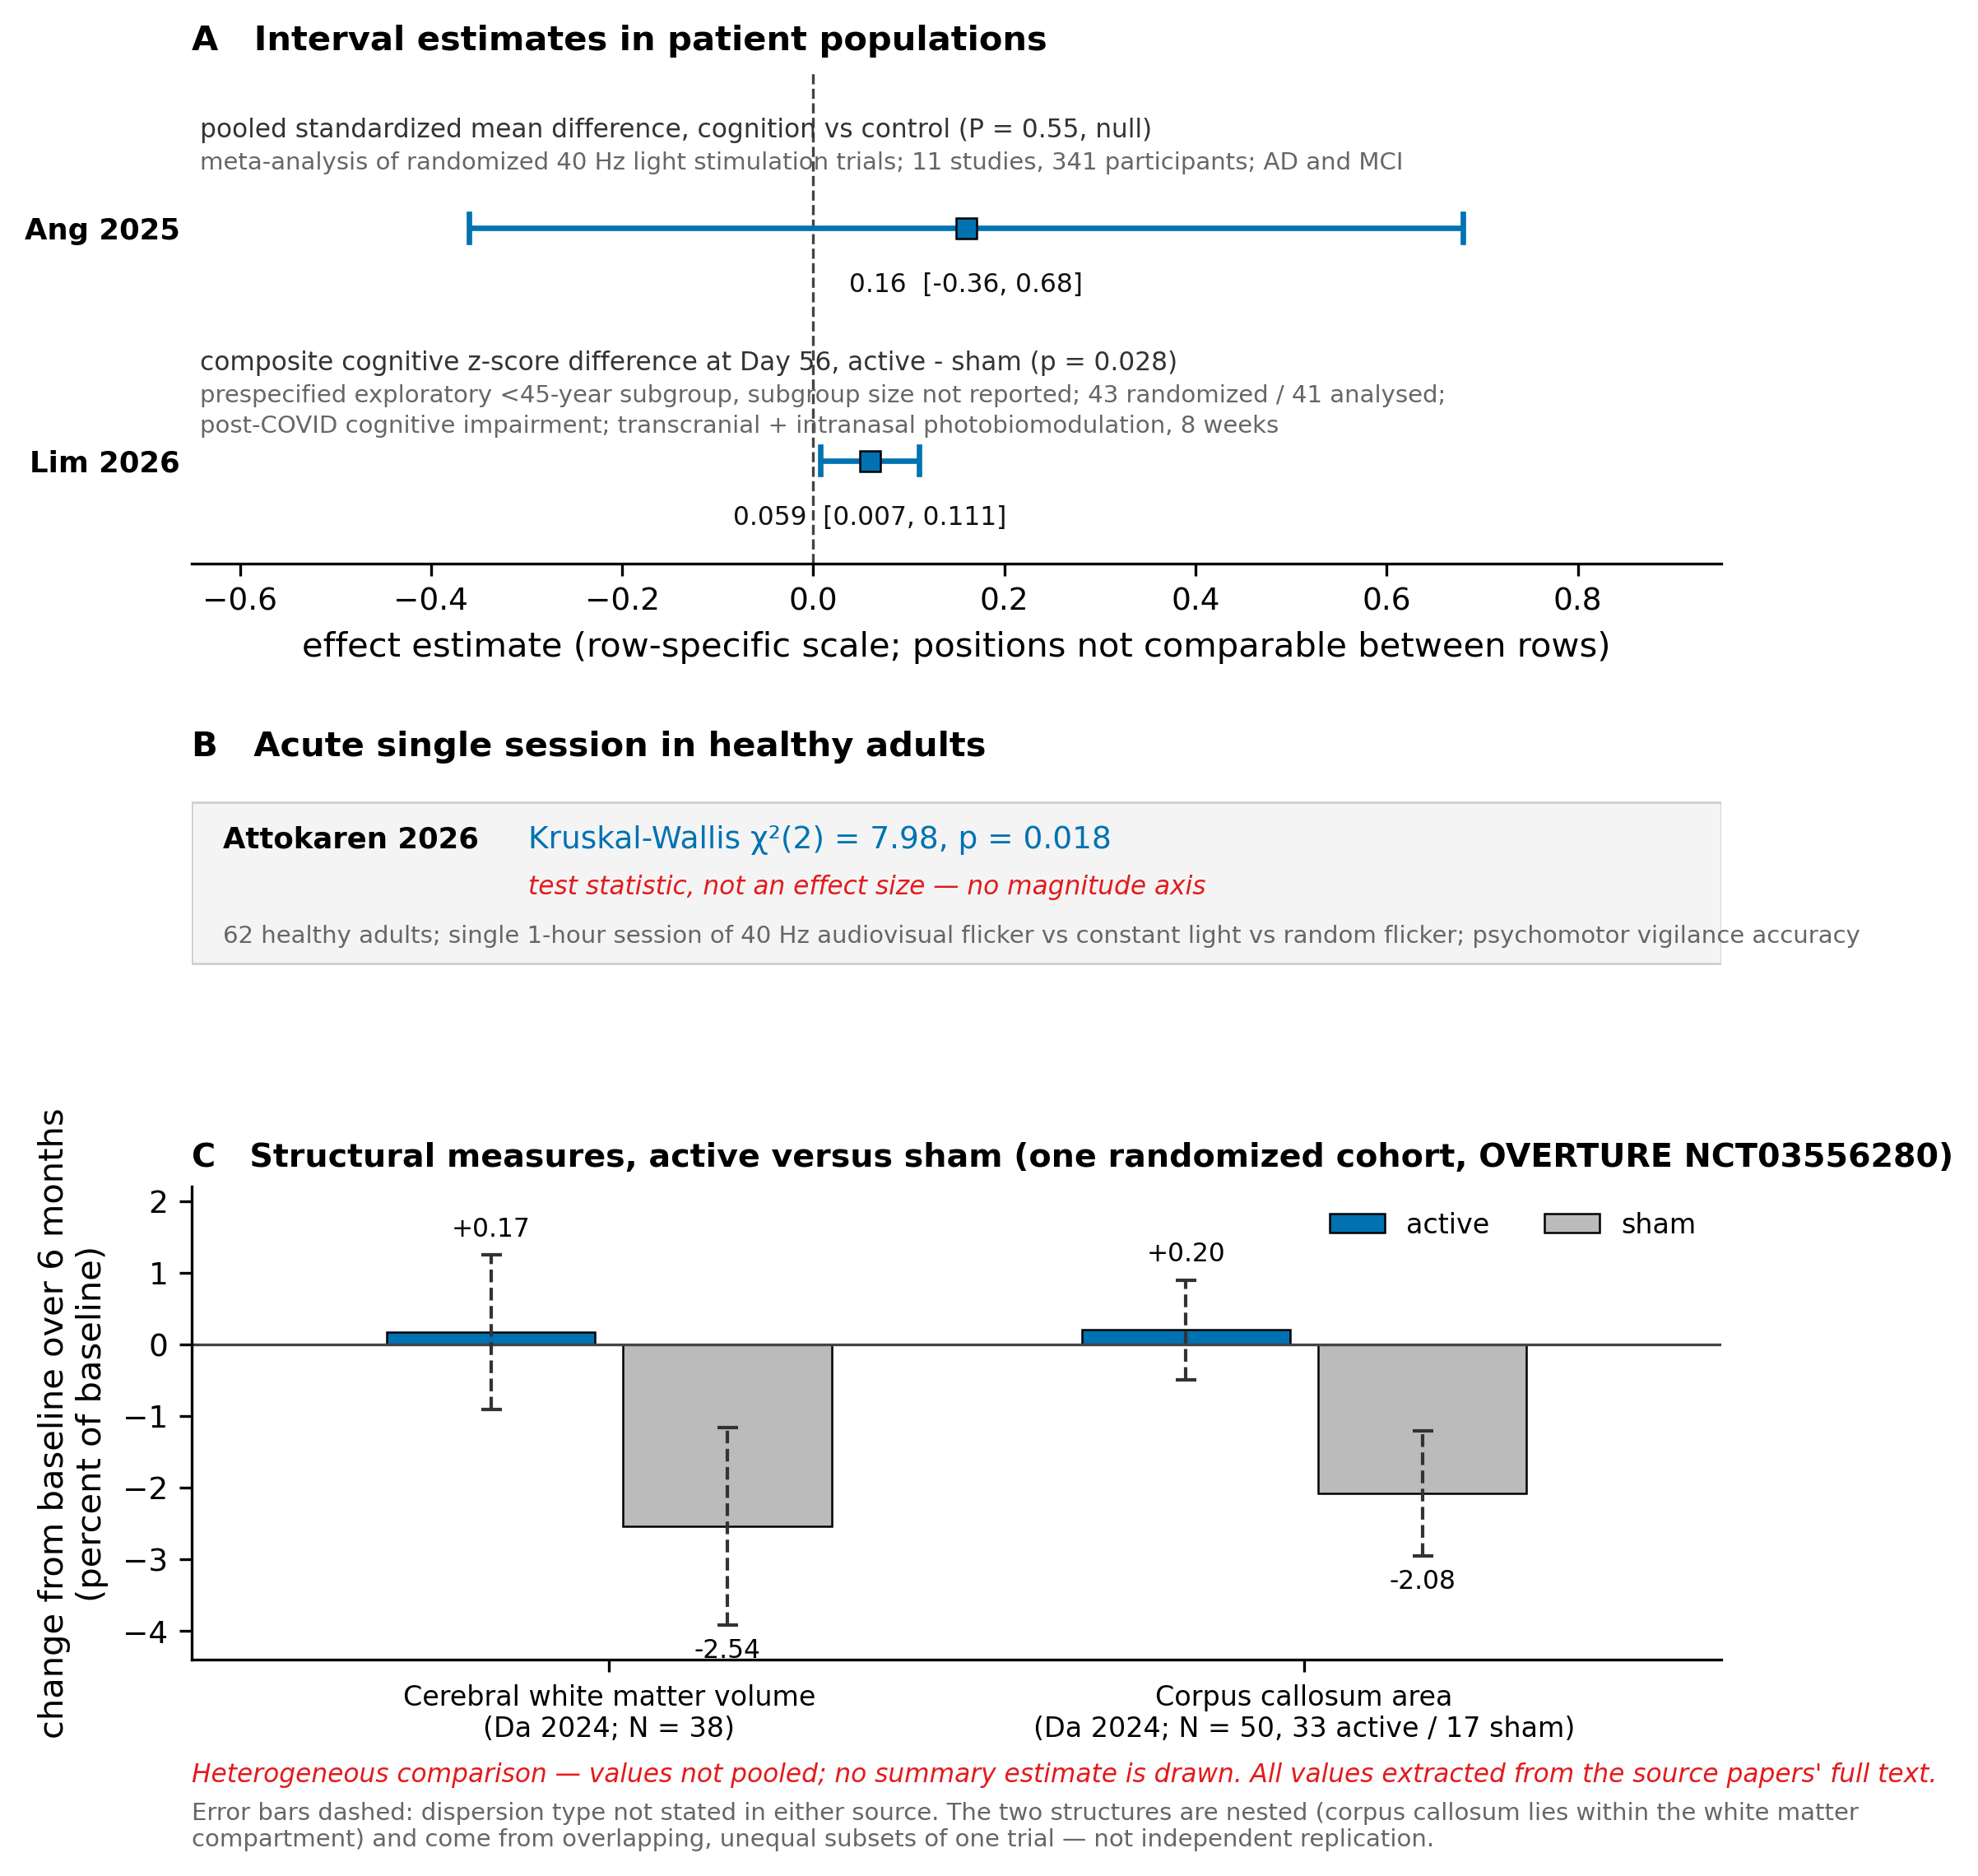
\includegraphics[width=\linewidth]{../figures/fig_sec10_gamma_stimulation_evidence_ladder.png}
\caption{\textbf{Gamma stimulation in humans, ordered by design.} (A) Sham- or control-referenced interval estimates in patient populations \citep{Ang2025,Lim2026}. (B) Acute single-session attention in healthy adults, shown as a test statistic with no magnitude axis \citep{Attokaren2026}. (C) Percent change from baseline over 6 months, active versus sham, for two structural measures \citep{Da2024a,Da2024b}. Ang 2025's SMD = 0.16 is a null finding (P = 0.55, 95\% CI crossing zero), not a small benefit. Lim 2026's 0.059 is an exploratory <45-year subgroup estimate; the trial's primary outcome was 0.043, p = 0.088, non-significant, and the subgroup's own size is not reported, so that row carries no weight. The two panel-A rows are on different scales (a pooled standardized mean difference and a raw composite z-score difference), are not pooled, and their positions on the axis are not comparable with one another; each row prints its own metric. Attokaren 2026's value is a Kruskal--Wallis test statistic, not an effect size, and comes from healthy adults after a single 1-hour session; it is shown in a separate panel with no magnitude axis. Sensory gamma entrainment (40 Hz audiovisual flicker) and near-infrared photobiomodulation (Vielight Neuro RX Gamma device) are distinct interventions; the photobiomodulation pulse rate is not stated in its abstract. Only Ang 2025 studies a dementia population. Sample sizes are as stated in each paper's abstract (341 pooled participants; 43 randomized / 41 analysed; 62 healthy adults). "Whole brain" in the row annotations is a label, not an equivalence: Lim 2026 delivered light to default-mode-network targets, the other entries drove the whole brain through the senses. In panel C, both measurements come from the same trial cohort (OVERTURE, NCT03556280) with overlapping participants (white matter subset N = 38; corpus callosum subset N = 50, 33 active / 17 sham) --- one trial reported twice, not independent replication; the corpus callosum is a component of the white matter compartment measured in the other entry, so the two percent changes are nested, not independent; one entry is a volume change, the other a cross-sectional area change, both expressed as percent of baseline; error terms are reproduced as published, the sources do not state whether they are SD or SEM, and for the corpus callosum sham arm the published $\pm$0.87\% cannot be distinguished from the $\pm$0.87\% the abstract attaches to the between-group difference; the corpus callosum analysis used Bayesian linear mixed-effects modelling, while the white matter analysis reports a significance test without naming its framework; rows are labelled by measured structure because both entries would otherwise appear as "Da 2024"; and the corpus callosum analysis describes its population as mild cognitive impairment or Alzheimer's disease, not mild-to-moderate Alzheimer's disease alone.}
\label{fig-sec10-gamma-stimulation-evidence-ladder}
\end{figure}

\subsection{Interneuron replacement and interneuron-directed gene therapy}
\label{sec-10-replacement}

Cell replacement is the only strategy in this section that puts new inhibitory neurons into a diseased network, and its quantitative strength is concentrated in epilepsy. Medial ganglionic eminence (MGE) progenitors grafted into the adult epileptic hippocampus reduced spontaneous electrographic seizure frequency by 92\%, to a reported frequency of 0.17 $\pm$ 0.09 in eight animals, with graft-derived cells characterised by patch clamp \citep{Hunt2013}; a clinical-grade human embryonic stem cell-derived MGE-type product suppressed mesiotemporal seizures after a single intrahippocampal dose, with most animals becoming seizure-free and surviving longer \citep{Bershteyn2023}; and a synthesis of neural stem cell graft outcomes in status epilepticus models collects reports that grafting limits the structural reorganisation accompanying those seizures --- a different graft class from the MGE-derived progenitors above, at review level rather than as a single primary experiment \citep{Wang2025c}. \ref{fig-sec10-cell-and-circuit-interventions} sets these graft and vector quantities side by side, each on its own axis. The cell source is tractable: human pluripotent stem cells can be directed to NKX2.1+ progenitors that yield parvalbumin- and somatostatin-expressing cortical interneurons with appropriate synaptic properties \citep{Maroof2013}, although those cells need roughly 30 weeks post-differentiation to acquire mature firing, with 5 of 7 recorded neurons identified as SST-positive \citep{Nicholas2013}. Two facts restrict what this means for neurodegeneration. First, the SST yield is a minority of the graft: transplanted MGE progenitors differentiated into 41.3 $\pm$ 2.8\% parvalbumin-positive, 21.6 $\pm$ 1.2\% somatostatin-positive and 7.7 $\pm$ 0.8\% nNOS-positive cells \citep{Wang2025a}, so a graft is an inhibitory-tone intervention rather than an SST-selective one. Second, the host models are mostly not Alzheimer models --- Fragile X \citep{Wang2025a}, status epilepticus \citep{Wang2025c}, early-life stress \citep{Lin2025} --- and the one amyloid-model graft retrieved here is a single study, reported both as a preprint \citep{Yokomizo2025b} and as a journal record carrying the quantitative result, in which transplanted progenitors integrated into APP/PS1 cortex and raised slow-oscillation power relative to vehicle-treated hosts \citep{Yokomizo2025a}. The limitation is that it stands alone, not that it is unpublished.

\begin{quote}
\noindent\textbf{Evidence Conflict}\par
\textbf{Do unmodified interneuron progenitors suffice in an amyloid host?} Transplantation into J20 hAPP mice reduced behavioural abnormalities only when the grafted MGE cells overexpressed Nav1.1; wild-type MGE grafts gave no benefit, which the authors read as a requirement for molecular optimisation in a hyperexcitable, amyloid-laden brain \citep{MartinezLosa2018}. Transplantation of unmodified embryonic interneuron progenitors into the hippocampal hilus of aged apoE4 knock-in and amyloid-model mice, by contrast, is reported to have restored normal learning and memory \citep{Tong2014}. Host model, graft site and amyloid burden all differ, so the disagreement is resolvable by method rather than by arbitration between results --- and it is precisely the variable, model construct, that \ref{sec-conflicts-limitations} identifies as the dominant predictor of reported interneuron phenotypes.

\end{quote}

Gene therapy addressed to interneurons has the better-characterised toolkit. An adeno-associated virus carrying the mDlx enhancer restricted expression almost exclusively to GABAergic cells, with \textasciitilde{}95\% of transgene-expressing cells co-expressing GAD67 \citep{Dimidschstein2016}, while a panel of candidate enhancers ranged from over 90\% to below 5\% parvalbumin specificity depending on which enhancer was used \citep{VormsteinSchneider2020} --- a spread that has not been independently replicated and that makes vector choice, not the concept, the determinant of selectivity. Payloads now include endogenous-locus activation by dCas9, which restored interneuron firing and attenuated febrile seizures in a Dravet model \citep{Colasante2020}, and antisense de-repression, where AAV9-AntagoNAT raised survival from 50\% to 84\% and cut febrile seizure susceptibility from 73\% to 7.7\% in \emph{Scn1a}+/$-$ mice \citep{Diaz2026}. Timing may constrain both: AAV gene replacement that worked neonatally produced no survival benefit at postnatal day 10 \citep{Chen2025b}, an unreplicated result whose authors note that the loss of benefit could equally reflect reduced viral coverage at the later age as a closing developmental window --- on the first reading it sets an uncomfortable timing constraint for a late-onset disease, on the second it sets none. The chemogenetic approach that would most directly test SST causality carries a ligand confound: clozapine-N-oxide (CNO) itself impaired object-location memory encoding whereas Compound 21 did not, with neither ligand altering overall neuronal or parvalbumin interneuron activity across dorsal hippocampal subregions, a result reported in a preprint \citep{Bunce2026}. What is missing is not replication of that confound but replication of the rescue experiments it threatens --- no published SST-interneuron chemogenetic rescue effect has been re-run here with a non-CNO ligand or with CNO-only controls. The one chemogenetic manipulation of a somatostatin-family population retrieved here went the other way, with repeated inhibition of cortistatin-expressing prelimbic neurons accelerating seizure kindling in female mice \citep{Salisbury2026}.

\begin{figure}[H]
\centering
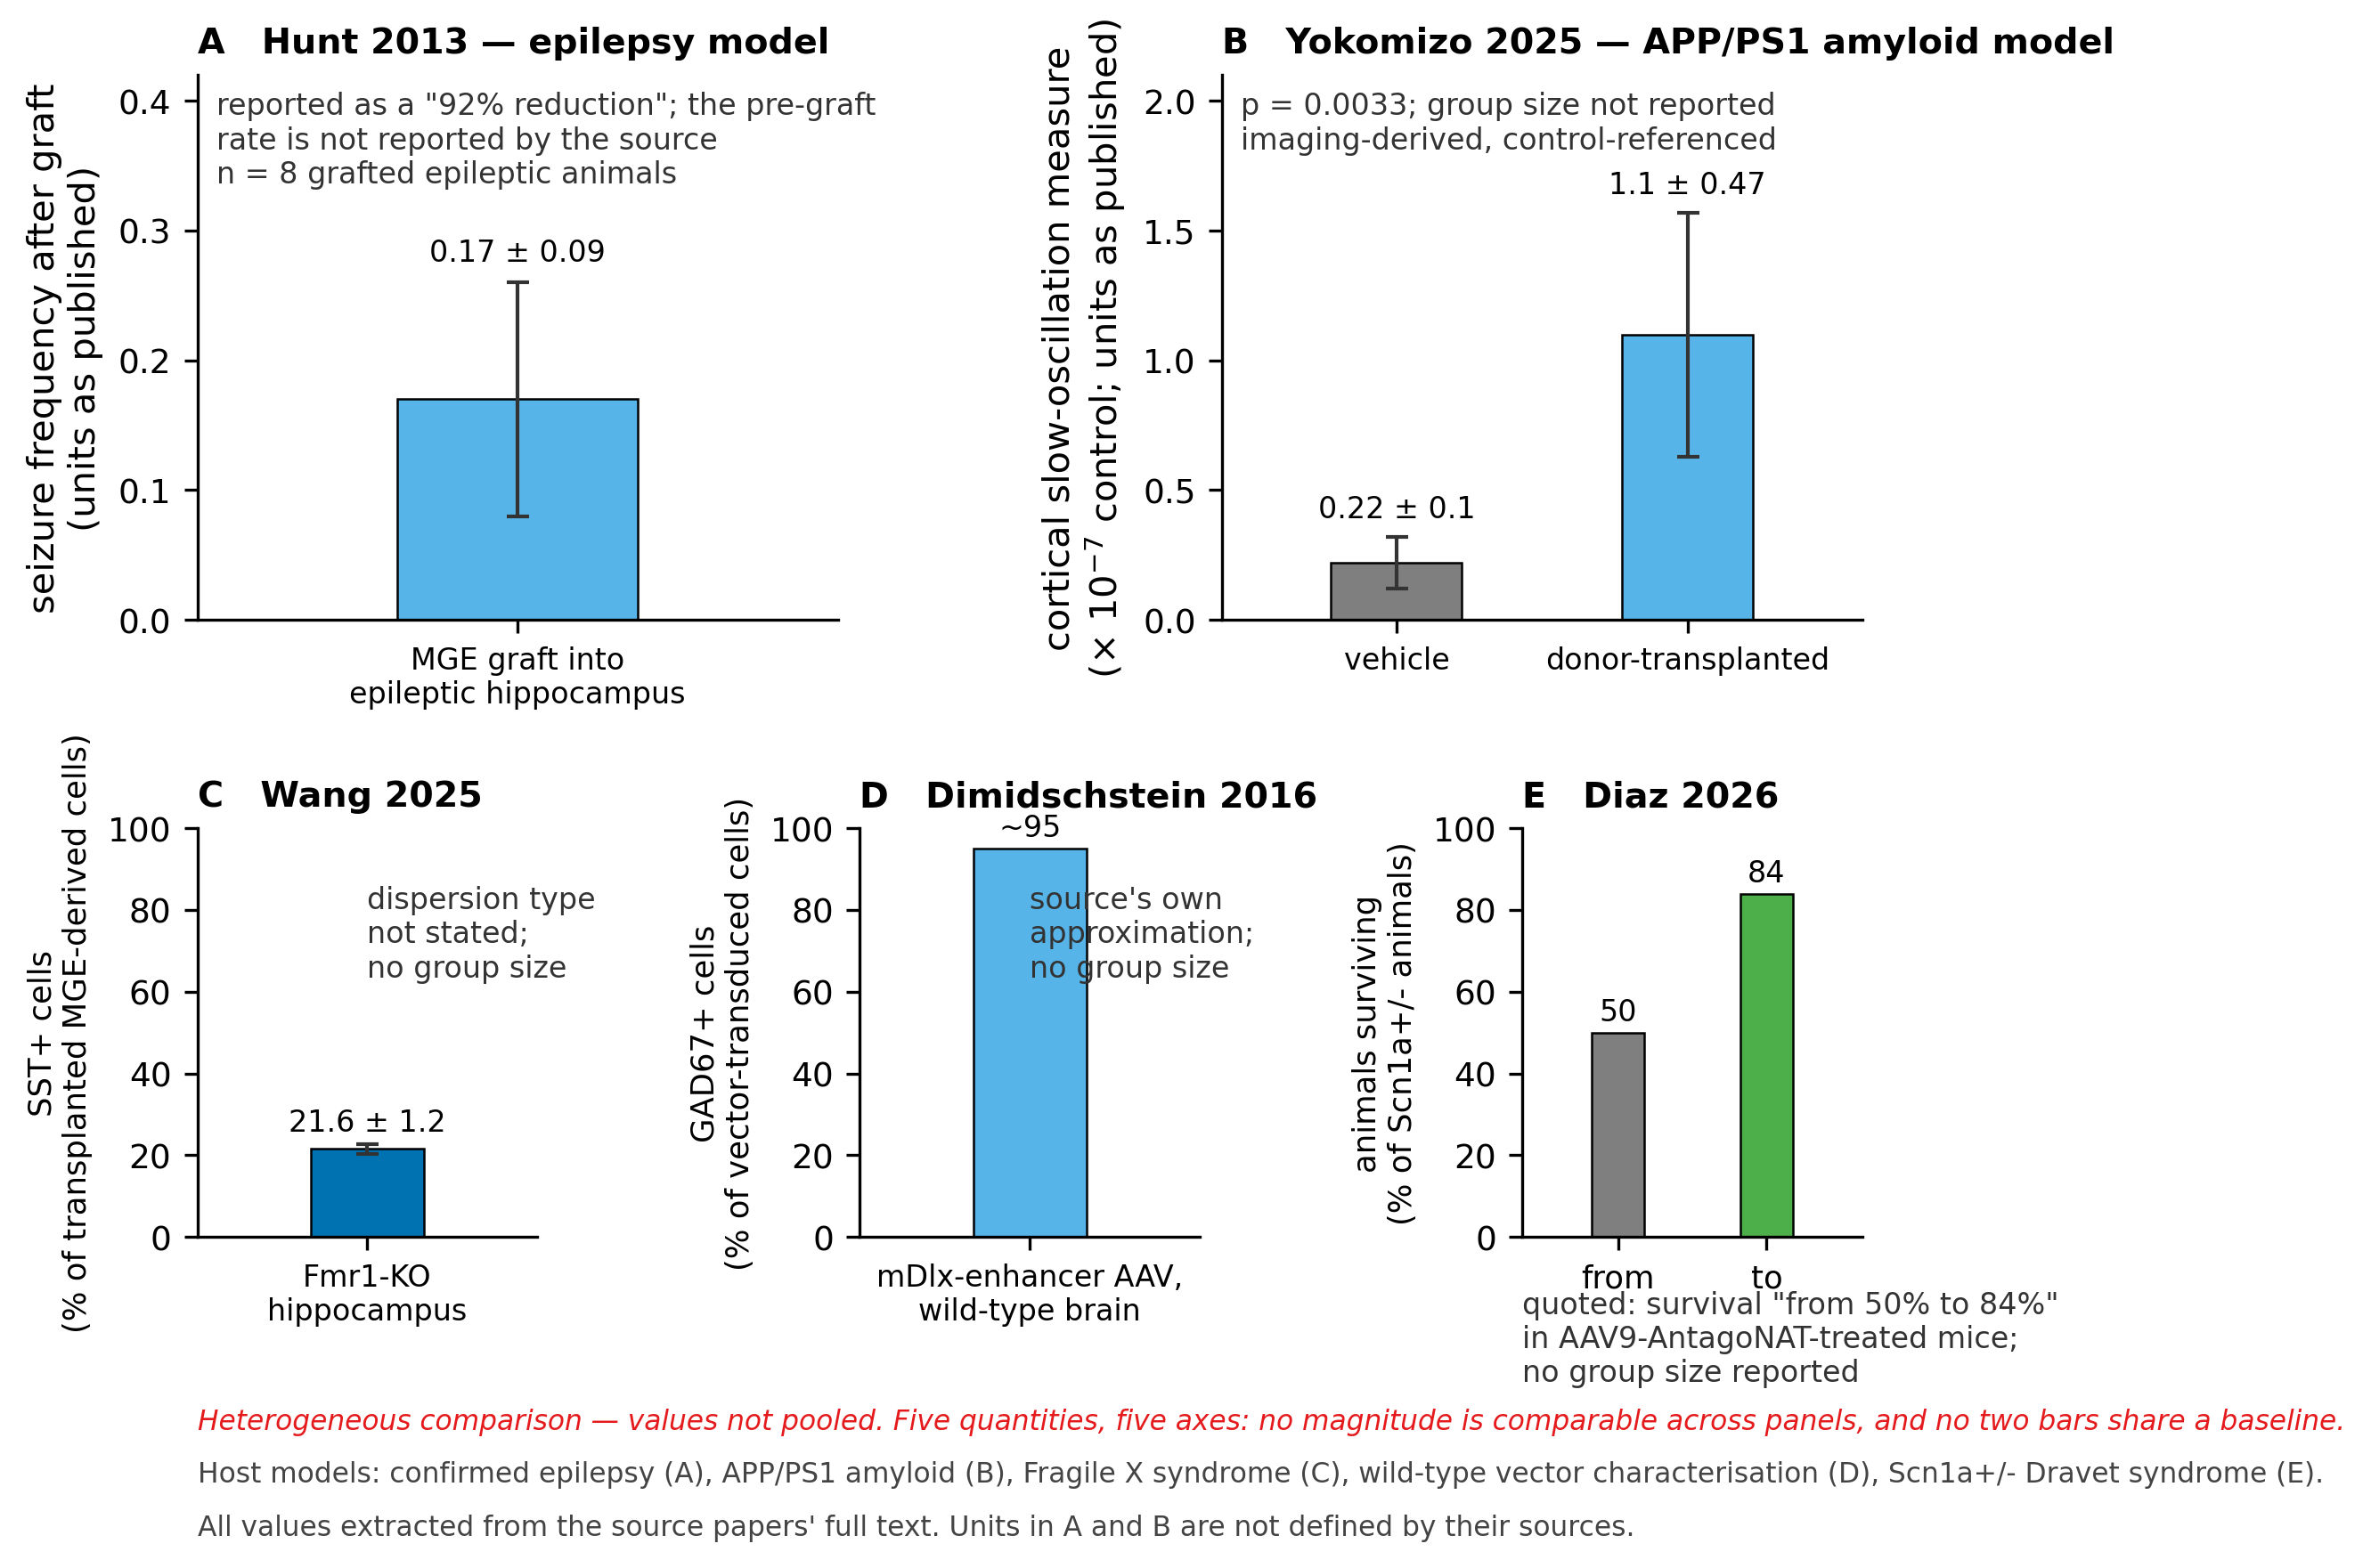
\includegraphics[width=\linewidth]{../figures/fig_sec10_cell_and_circuit_interventions.png}
\caption{\textbf{Cell and vector interventions: five quantities, five axes.} (A) Electrographic seizure frequency in grafted epileptic animals \citep{Hunt2013}. (B) Cortical slow-oscillation measure, donor-transplanted versus vehicle APP/PS1 \citep{Yokomizo2025a}. (C) SST+ fraction of transplanted MGE-derived cells \citep{Wang2025a}. (D) GAD67+ fraction of vector-transduced cells \citep{Dimidschstein2016}. (E) Survival of treated \emph{Scn1a}+/$-$ animals \citep{Diaz2026}. The panels use independent axes and independent units; no shared scale is implied and the magnitudes are not comparable. Different host pathologies: epilepsy confirmed at the time of grafting versus APP/PS1 amyloid deposition; only the APP/PS1 entry is a neurodegeneration model. Different graft and recording territories (hippocampus versus cortex); in the epilepsy study the seizure effect was site-specific --- amygdala grafts did not alter seizure activity. Group n is stated for the epilepsy entry (n = 8); the amyloid entry's source states none, in its result sentence or its abstract. The control seizure rate is not shown: the source states a 92\% reduction and a grafted frequency of 0.17 $\pm$ 0.09, and does not report the pre-graft rate, which cannot be derived from those two values. Both axes in A and B are labelled "units as published": the seizure-frequency unit is not given in its source, and the oscillation quantity is published as "$\times$ 10$^{-}$$^{7}$ control", which may be a normalisation to control rather than an absolute power. The slow-oscillation measurements are reported by their source as obtained with in vivo multiphoton calcium imaging and voltage-sensitive dye imaging; the panel-B quantity is an imaging-derived, control-referenced measure, not an electrophysiological power spectrum. In C--E the three percentages have three different denominators --- transplanted MGE-derived cells, animals, vector-transduced cells --- and are not a common efficacy scale; each occupies a separate sub-panel whose axis label names its denominator, and no two bars share a baseline. The SST+ fraction and the GAD67+ fraction differ by a level of the marker hierarchy --- a graft-composition subtype fraction versus a pan-interneuron vector-specificity fraction --- and measure different things; they are shown in separate sub-panels so that their heights are not compared. Interventions differ in kind: MGE-derived GABAergic precursor grafting, AAV9 antisense gene therapy, and a viral targeting vector. None of the studies in C--E uses a neurodegeneration model; the models are Fragile X syndrome, Dravet syndrome and wild-type vector testing. No entry in C--E reports a group size in its source sentence and the abstracts supply none, so no bar is weighted. The neuronal-loss quantities available for these models come from a narrative review's account of another laboratory's primary data and are not plotted here.}
\label{fig-sec10-cell-and-circuit-interventions}
\end{figure}

\subsection{Lowering network excitability pharmacologically}
\label{sec-10-excitability}

The excitability-lowering literature is the best-designed in this section and the clearest about what it has not achieved. Its clinical rationale is that patients with amnestic mild cognitive impairment (aMCI) or Alzheimer's disease (AD) who also have epilepsy or subclinical epileptiform activity decline earlier, cognitive decline beginning before 65 years in 50\% of aMCI-epilepsy cases versus 21\% without (P = .051) and in 51\% versus 26\% of AD cases (P = .002) \citep{Vossel2013} --- the AD comparison carries the weight, the aMCI one does not reach the conventional threshold. The target engagement result is the strongest of its kind: low-dose levetiracetam reduced hippocampal hyperactivity and improved the hyperactivity-sensitive pattern-separation task while leaving standard delayed-recall measures unchanged in the same 17 patients \citep{Bakker2012} --- a pre-specified direction with a reported null on the non-targeted measure. The drug's mechanism is presynaptic, acting through SV2A, since brain membranes from SV2A-null mice do not bind a tritiated levetiracetam derivative \citep{Lynch2004}, with its in vivo anticonvulsant effect abolished by a benzodiazepine-site inverse agonist \citep{Rigo2002}. Scaling up, the randomized crossover trial found no overall cognitive change (NIH-EXAMINER mean difference 0.07 points, 95\% CI $-$0.18 to 0.32, P = .55) but a 7.4-point Stroop interference improvement (95\% CI 0.2--14.7) confined to the prespecified epileptiform-activity subgroup \citep{Vossel2021}; a synthesis of five clinical studies found cognitive change reported in four \citep{Mohamadi2025}. Seizures themselves respond well --- 72.7\% of a 22-patient prodromal AD cohort achieved seizure freedom and 95.4\% a $\geq$50\% reduction \citep{Cretin2026} --- against responder rates of 30--50\% in unselected epilepsy trials, where the companion benchmark, a 20--30\% median reduction in seizure frequency, is a different quantity and shares no denominator with a proportion of patients \citep{Loscher2021}. Which model is used matters: as reviewed in a case for screening antiseizure drugs across several Alzheimer models, kindling outcomes diverge between APP/PS1 and PSEN2-N141I lines, an account of other groups' experiments whose primary reports were not retrieved here \citep{Barbour2025}. \ref{fig-sec10-excitability-lowering-outcomes} places these three outcome types on three separate axes, which is the only honest way to show them together. The gap this leaves is the one that matters for the thesis: symptom control is demonstrated, disease modification is not.

\begin{quote}
\noindent\textbf{Evidence Conflict}\par
\textbf{Does lowering excitability change the cognitive trajectory?} The randomized crossover trial reports no overall benefit on its primary composite \citep{Vossel2021}, while a pharmacoepidemiologic analysis drawing on a database of more than 75 million adults aged 55 or older associates sodium-channel-blocking antiseizure medications with a 27\% lower hazard of incident all-cause dementia (HR = 0.73, 95\% CI 0.61--0.88) and a 34\% lower hazard of Alzheimer's disease, relative to levetiracetam/brivaracetam \citep{FerreiraAtuesta2026}. Drug class, design and outcome definition all differ --- an SV2A ligand tested on short-term cognition against sodium channel blockers assessed on long-term incidence, with levetiracetam serving as index drug in one and reference drug in the other --- so this is resolvable by method rather than a contradiction of results, and the observational estimate carries the confounding-by-indication that its design implies.

\end{quote}

\begin{figure}[H]
\centering
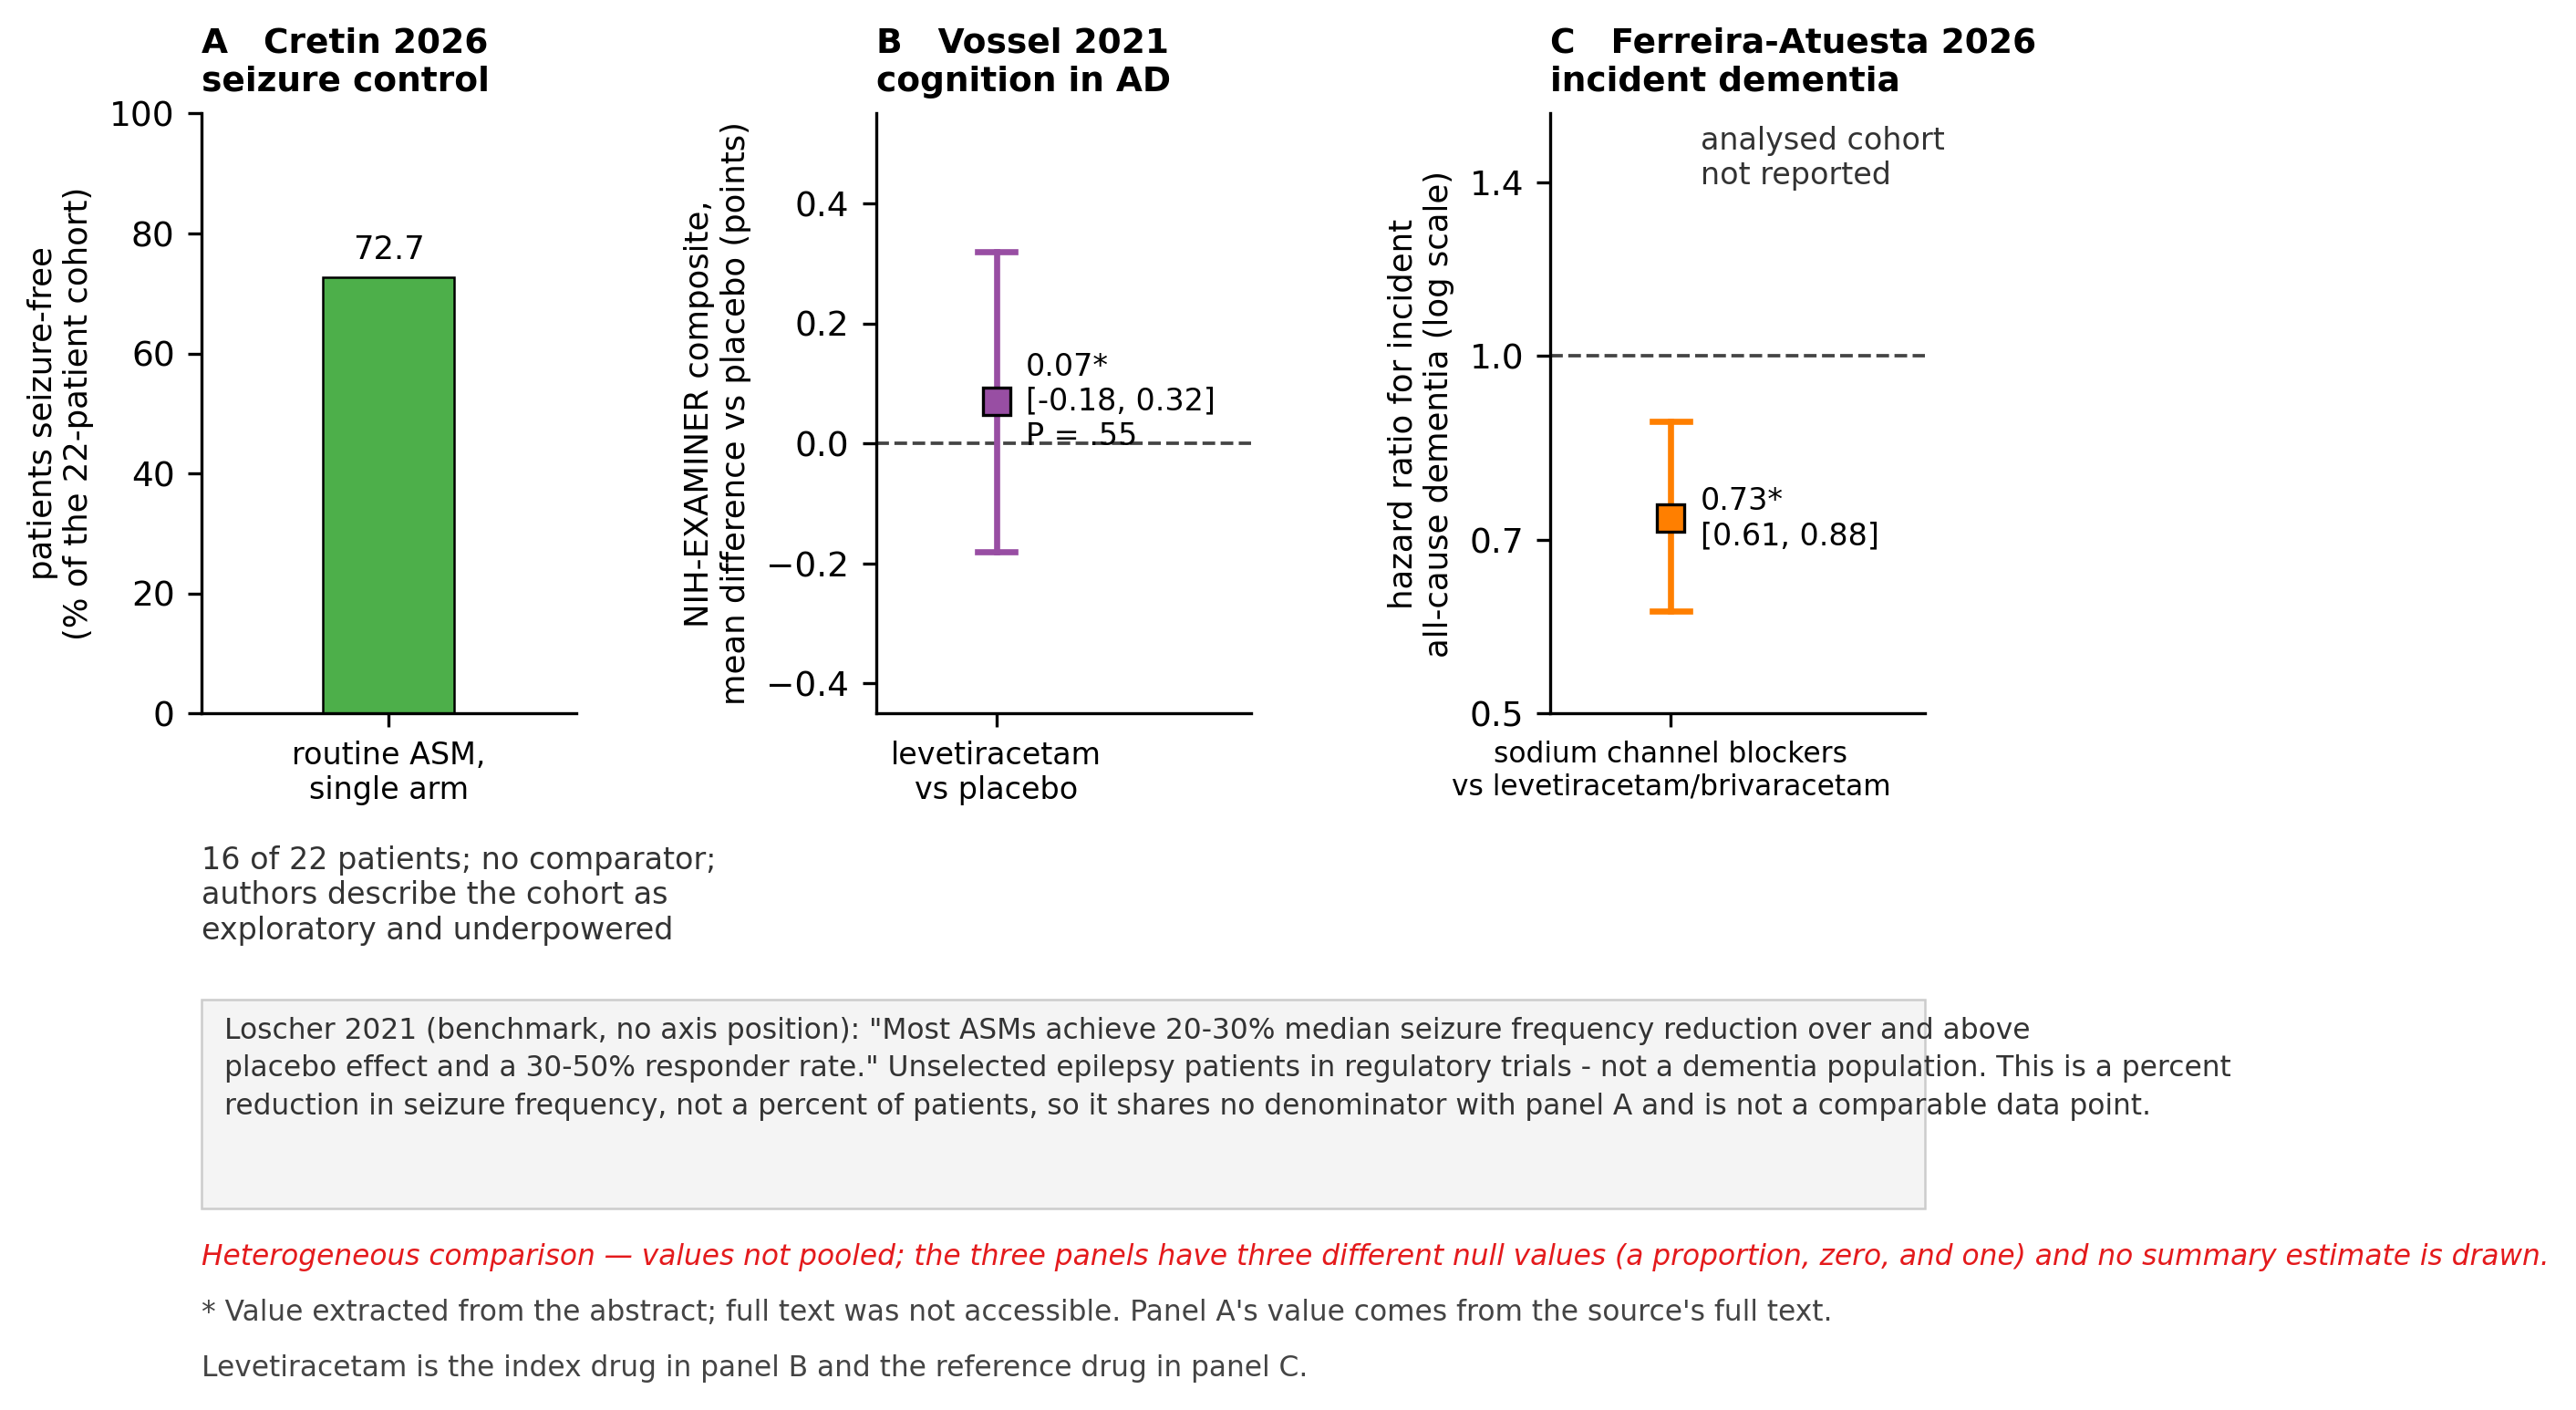
\includegraphics[width=\linewidth]{../figures/fig_sec10_excitability_lowering_outcomes.png}
\caption{\textbf{Excitability-lowering drugs: three outcome types, three axes.} (A) Proportion of patients seizure-free in an epileptic prodromal-AD cohort \citep{Cretin2026}. (B) NIH-EXAMINER composite, mean difference versus placebo \citep{Vossel2021}. (C) Hazard ratio for incident all-cause dementia against an active comparator \citep{FerreiraAtuesta2026}. The margin quotes a review-level benchmark \citep{Loscher2021} that has no position on any axis. Panels use different outcome types and are not on a shared scale: a cognitive composite difference in points, a proportion of patients seizure-free, a hazard ratio (null = 1) and a median percent seizure-frequency reduction. The reported n of 75 million is the size of the source database of adults aged 55+, not the analysed cohort of patients with late-onset unexplained epilepsy, which the source does not state; the figure carries "analysed cohort not reported". The hazard ratio 0.73 is against an active comparator (levetiracetam/brivaracetam), not placebo; its own source notes that individual agents such as phenytoin, carbamazepine and lamotrigine showed divergent safety and efficacy profiles. The levetiracetam value of 0.07 points is a null primary outcome (P = .55); the trial's positive signals were restricted to the prespecified epileptiform-activity subgroup. The 72.7\% seizure-freedom figure is a single-arm proportion in 22 patients (16 of 22) from a cohort its authors describe as exploratory and underpowered; in the abstract that caveat is attached to the cohort's cognitive-decline and medication comparisons rather than specifically to the seizure-freedom proportion. The 20--30\% figure is a review-level generalization across epilepsy regulatory trials in unselected epilepsy patients, not a dementia population. It is a percent reduction in seizure frequency, not a percent of patients, so it shares no denominator with the 72.7\% seizure-freedom proportion; it is quoted as text with no position on any axis and is not a comparable data point. The observation that individual agents showed divergent safety and efficacy profiles belongs to the hazard-ratio source, not to the review that supplies the 20--30\% benchmark. Levetiracetam is the index drug in the cognitive panel and the reference drug in the dementia-incidence panel.}
\label{fig-sec10-excitability-lowering-outcomes}
\end{figure}

\subsection{Neuromodulation of circuits: fornix stimulation as a cautionary case}
\label{sec-10-neuromodulation}

Fornix deep brain stimulation shows the design gradient in a single programme. The open-label phase I study reported an early and striking reversal of temporal and parietal glucose hypometabolism maintained through 12 months of continuous stimulation, with possible slowing of decline in some patients \citep{Laxton2010}. The randomized double-blind trial that followed found that the primary measures, ADAS-cog-13 and CDR-SB, did not differentiate active from sham after 12 months \citep{Targum2021}. Chronic intracranial recordings then supplied a mechanism for the null: continuous stimulation overdrove fornix-to-hippocampus connectivity while attenuating hippocampal feedback, which the authors characterise as an electrical lesion \citep{Stanslaski2026} --- a single recent report with no replication. Interpreting volumetric endpoints in this programme requires the natural-history baseline, in which 67.5\% of 40 comparison patients lost hippocampal volume over 12 months at a 3\% threshold, 32.5\% were unchanged and none gained \citep{Germann2025}; the wider surgical literature reports both attenuation of decline and postoperative adverse effects \citep{Swietlik2024}. Non-invasive stimulation faces the same gradient at smaller scale: two weeks of precuneus rTMS produced a domain-selective episodic memory improvement \citep{Koch2018}, dual-target cerebellar TMS with striatal temporal-interference stimulation improved working-memory accuracy during distraction in mild cognitive impairment with Lewy bodies, but not under high load \citep{Nencha2026}, and transcranial direct current stimulation has a measurable neurochemical footprint --- anodal stimulation lowers local GABA, cathodal stimulation lowers glutamatergic activity \citep{Stagg2009}, and baseline sensorimotor GABA concentration predicts motor performance (r = 0.64, p = 0.03, uncorrected) \citep{Stagg2011} --- though these two magnetic resonance spectroscopy reports share a senior author and are convergence within one programme rather than independent replication, the standard applied to the agonist series above. Yet current trials remain feasibility-scale, one powered at 36 participants \citep{Kuo2026}. None of these methods reads out SST-cell function specifically, although paired-pulse TMS does index inhibitory circuit integrity in neurodegeneration: short-latency afferent inhibition is markedly weaker in Alzheimer's disease than in age-matched controls (responses reduced to 85.7 $\pm$ 15.8\% of test size versus 45.3 $\pm$ 16.2\%) \citep{DiLazzaro2002}, and absent short-interval intracortical inhibition has 97\% sensitivity for ALS \citep{Vucic2012}.

\begin{quote}
\noindent\textbf{Evidence Conflict}\par
\textbf{Does fornix stimulation activate or functionally lesion the hippocampal circuit?} Metabolic imaging in the uncontrolled phase I cohort was read as circuit activation \citep{Laxton2010}; directed electrophysiological connectivity in chronically implanted patients indicates the opposite, that continuous stimulation disrupts bidirectional fornix--hippocampus communication \citep{Stanslaski2026}. The dimension is inference from metabolism versus inference from directed connectivity, and the question is open; the randomized sham-controlled null \citep{Targum2021} is consistent with either reading, which is why the mechanistic recordings matter more than the trial result.

\end{quote}

\subsection{What would make an SST-targeted therapy testable}
\label{sec-10-testable}

Three requirements follow from the preceding evidence, and each names an experiment that was not retrieved by these searches rather than one that failed. First, an SST-selective manipulation inside a disease model: the entrainment literature drives parvalbumin circuitry, as the survey that reports the medial-septal experiment describes \citep{Zhang2024a}, grafts deliver mixed populations in which SST cells are a minority \citep{Wang2025a}, and the chemogenetic tools that could isolate the class carry a ligand confound whose consequences for published rescue effects have not been tested with a non-CNO ligand here \citep{Bunce2026}, so the "tractable target" framing is an extrapolation and should be read as one. Second, a brain-penetrant SSTR4 agonist with a pharmacodynamic marker: the existing in vivo results come from one compound and one programme \citep{Sandoval2011,Sandoval2012,Sandoval2013,Sandoval2019}, the approved analogue class cannot reach the relevant subtype \citep{Patel1999}, and the structural determinants of subtype selectivity are known well enough to design against \citep{Zhao2022}. Brain entry of that compound has been measured directly (entry rate K(i) = 0.25 $\mu$l/g min, with about 93\% associated with the parenchymal component) \citep{Sandoval2011}, and an amyloid-model efficacy study exists within the same programme, with learning improved and soluble A$\beta$ oligomers reduced in APPswe Tg2576 mice \citep{Sandoval2013}; what is missing is a concentration-at-target measurement tied to efficacy, an independent programme, and any tau-model study. Third, an endpoint matched to the lesion: trials in this literature test global cognition, yet the circuit function attributable to SST cells (\ref{sec-sst-identity}, \ref{sec-circuit-consequences}) is dendritic inhibition and the coordination of non-rapid-eye-movement oscillations, which is where graft-mediated rescue of slow oscillations \citep{Yokomizo2025b} and the subtype-divergent EEG entrainment response \citep{Chan2025} point, and which \ref{sec-human-evidence} identifies as lacking a biomarker-grade readout; \ref{sec-conclusion} returns to these three requirements as the conditions under which the causal question could be answered. No head-to-head comparison of gamma entrainment, transplantation, antiseizure pharmacology and SSTR agonism on a common endpoint in a single model was retrieved either, so the apparent breadth of this field conceals an absence of comparative evidence.

Two features of the evidence behind this section limit how firmly any of it can be stated. Retrieval was dominated by one literature database with no citation chasing, so every statement above that an experiment was not found is a statement about these searches and not about the field; disconfirming-evidence searches were capped per query, so the reported nulls are a top-relevance sample rather than a census. Full text was available for 58 of the 86 records behind this section, with the shortfall concentrated in older closed-access material, and the replication ceiling here is low: most findings carry no identified replicating study, which is why no therapeutic claim in this section is called replicated unless the replicating work is named. The therapeutic failures catalogued here are not randomly distributed. They cluster exactly where the causal chain was extrapolated rather than demonstrated --- from parvalbumin to SST, from epilepsy host to amyloid host, from rodent molecular endpoint to patient cognition, from a programme's internal convergence to independent replication. \ref{sec-conflicts-limitations} anatomises those extrapolations across the whole review.

\section{Conflicting Evidence, Model Limitations, and Open Questions}
\label{sec-conflicts-limitations}

The interventions reviewed in \ref{sec-therapeutics} failed most clearly where the causal chain had been extrapolated rather than demonstrated: from a reduced somatostatin signal, to a lost cell, to a circuit lesion a receptor agonist or an entrainment protocol might reverse. The reasons that chain was never closed are methodological, and they are visible in the primary literature. Reported change in the somatostatin signal runs from no detectable change in cell number \citep{Futacsi2025} and no detectable change in density \citep{Sos2020}, through 63\% of hilar somatostatin-immunoreactive neurons surviving at the septal end and 21\% at the temporal end after kainate \citep{Jolkkonen1997}, to decreases of 57\% and 61\% in perirhinal cortex whose status as cell counts or as densities the retrieved text does not establish \citep{SanchezMejias2019}. The spread tracks counting design only in part: within design-based stereology the reported values run from no change \citep{Futacsi2025,Sos2020} to frank degeneration \citep{Loreth2012}, and the immunoreactive readouts extend to those perirhinal decreases \citep{SanchezMejias2019}. The one design here that identifies the cells independently of the peptide, genetic fate mapping, reports a statistically significant but small reduction \citep{Drake2024}. A current synthesis still presents early excitation-inhibition imbalance as driven by loss \emph{or} dysfunction of somatostatin and parvalbumin interneurons without resolving which \citep{Okechukwu2026}, while the counting literature warns that neuron-number estimates for one structure diverge between investigators using nominally the same method \citep{HerculanoHouzel2015}.

\subsection{Measurement decides the answer}
\label{sec-11-measurement}

The quantitative core of the problem is set out in \ref{fig-sec11-measurement-determines-the-answer}. Design-based stereology in TgF344-AD rats at 7-8 months found no change in the number of parvalbumin-, calretinin- or somatostatin-immunoreactive neurons, with reduction restricted to cholecystokinin cells \citep{Futacsi2025}; genetic fate mapping in a DGC-Pten knockout mouse found hippocampal eGFP-SST interneuron density reduced from 2,176 $\pm$ 97 to 1,901 $\pm$ 68 cells/mm3 (p = 0.0402) --- a density measure, which in a model with an expanded dentate molecular layer is not interchangeable with a change in cell number, and a change of a different order from the marker-based reports \citep{Drake2024}; and in the same amyloid literature a knock-in line carrying APP at endogenous dosage showed no significant change in somatostatin interneuron density in CA1 stratum oriens at 24 months, against a wild-type arm of 300 (270-350) cells/mm3 in 3 mice \citep{Sos2020}. Immunoreactivity counts return much larger numbers: 57\% and 61\% decreases in somatostatin-positive neurons in perirhinal areas 36 and 35 of 6-month-old APP/PS1 mice, alongside 91\% in Braak V-VI human cases \citep{SanchezMejias2019}, and after kainate-induced seizures only 63\% of hilar somatostatin-immunoreactive neurons surviving at the septal end of the rat hippocampus and 21\% at the temporal end \citep{Jolkkonen1997}. The one study here whose denominator is a pan-GABAergic population rather than the somatostatin population reported that kainate-treated rats lose 13\% of their GAD-positive dentate cells, of which 83\% of the missing cells were somatostatin-immunoreactive, against 52\% loss of GAD-negative hilar neurons (putative mossy cells) \citep{Buckmaster1999}. Two amyloid models analysed with one stereological protocol in a single laboratory gave opposite answers - about 30\% fewer calretinin-positive and more than 40\% fewer parvalbumin-positive neurons in plaque-bearing 5XFAD mice, no detectable reduction in the non-plaque-forming Tg4-42 line \citep{Giesers2020} - while stereology in a triple-transgenic overexpression line found frank degeneration of GABAergic septo-hippocampal projection neurons and their interneuron targets \citep{Loreth2012}. Neither sorting resolves the spread. Within design-based stereology the values run from no change \citep{Futacsi2025} through reductions of about 30\% in calretinin and more than 40\% in parvalbumin populations \citep{Giesers2020} to frank degeneration of GABAergic septo-hippocampal neurons and their interneuron targets in a triple-transgenic overexpression line \citep{Loreth2012} --- the direct counterpart of the endogenous-dosage knock-in null \citep{Sos2020}, from which it differs in construct rather than readout; within immunoreactive soma counts they run from that same null to decreases of 57\% and 61\% \citep{SanchezMejias2019}. Counting design and construct class each account for part of the spread, and no entry in this set controls both.

Ageing sets the scale against which any disease effect must be read, and it supplies the first clean case of two laboratories contradicting each other over the same molecule and species. Pre-prosomatostatin mRNA in 25-month-old rats fell by 49\% in frontal cortex, 80\% in parietal cortex and 69\% in striatum with no change in beta-actin gene expression, yet showed no statistical difference in hypothalamus \citep{Florio1991}; relative somatostatin gene expression, somatostatin mRNA against poly A+ RNA, in male Fischer 344 rats was unchanged in cortex across 3-4, 12-14 and 22 months (0.54 $\pm$ 0.11, 0.60 $\pm$ 0.08, 0.51 $\pm$ 0.04) but roughly 50\% of young levels in hypothalamus, which in situ hybridisation attributed to decreased expression within specific nuclei rather than to loss of somatostatin-containing neurons \citep{SONNTAG1990}. Each study's decline is the other's null, in the other's region. Aged rat hippocampus shows interneuron marker transcripts declining differentially and inversely tracking alpha1 GABA-A subunit upregulation \citep{Vela2003}, and both somatostatin mRNA and immunopositive cell number falling while parvalbumin number is preserved \citep{Gavilan2007}. Marker signal and cell presence also dissociate within one tissue: somatostatin-immunoreactive axons were exuberant in the sea lion dentate gyrus despite loss of immunopositive hilar somata \citep{Buckmaster2014}, a large Dlx-expressing population survives but turns hypoactive in pilocarpine epilepsy \citep{Matringhen2025}, and somatostatin and parvalbumin immunolabelling was indistinguishable from wild type in Huntington's models carrying prominent nuclear inclusions \citep{Menalled2000}. A marker reduction of disease magnitude is therefore available from ageing, axonal redistribution or functional silencing alone.

\begin{quote}
\noindent\textbf{Evidence Conflict}\par
\textbf{Magnitude of somatostatin interneuron depletion after kainate-induced seizures.} \citet{Buckmaster1999} attribute 83\% of missing GAD-positive dentate neurons to somatostatin-immunoreactive cells while reporting only 13\% loss of the GAD-positive population; \citet{Jolkkonen1997} report 63\% survival of somatostatin-immunoreactive hilar neurons at the septal end and 21\% at the temporal end. The disagreement is in the denominator and the septotemporal sampling position rather than in the biology. \textbf{Whether genetic reporter labelling confirms or refutes apparent somatostatin depletion} turns on the disease model rather than on the labelling strategy, and the two reports are worth stating side by side: labelling GABAergic interneurons genetically, by crossing R6/2 Huntington mice to a GAD2-Cre driver and a Cre-dependent tdTomato reporter, showed that reduced somatostatin and vasoactive intestinal peptide marker immunoreactivity was not accompanied by loss of the labelled cells \citep{Voelkl2022}, whereas eGFP-SST fate mapping in a Pten/mTOR epilepsy model found the labelled population itself reduced in density \citep{Drake2024}. Both identified cells independently of the peptide, so the divergence tracks the disease model rather than the labelling strategy; the Huntington result is a single report in the material retrieved here. \textbf{Whether amyloid pathology reduces somatostatin interneuron number} remains open: stereology in TgF344-AD rats found no change in somatostatin-immunoreactive cell number \citep{Futacsi2025}, whereas counts in APP/PS1 mouse olfactory bulb reported decreased somatostatin-positive cells and increased parvalbumin cells, with the calretinin result stated inconsistently inside that paper, whose summary reports an increase in transgenic animals while its co-localisation section reports a decrease \citep{DeLaRosaPrieto2016}; species, construct, region and counting method all differ between them, and no study resolving them within one laboratory was retrieved by these searches.

\end{quote}

\begin{figure}[H]
\centering
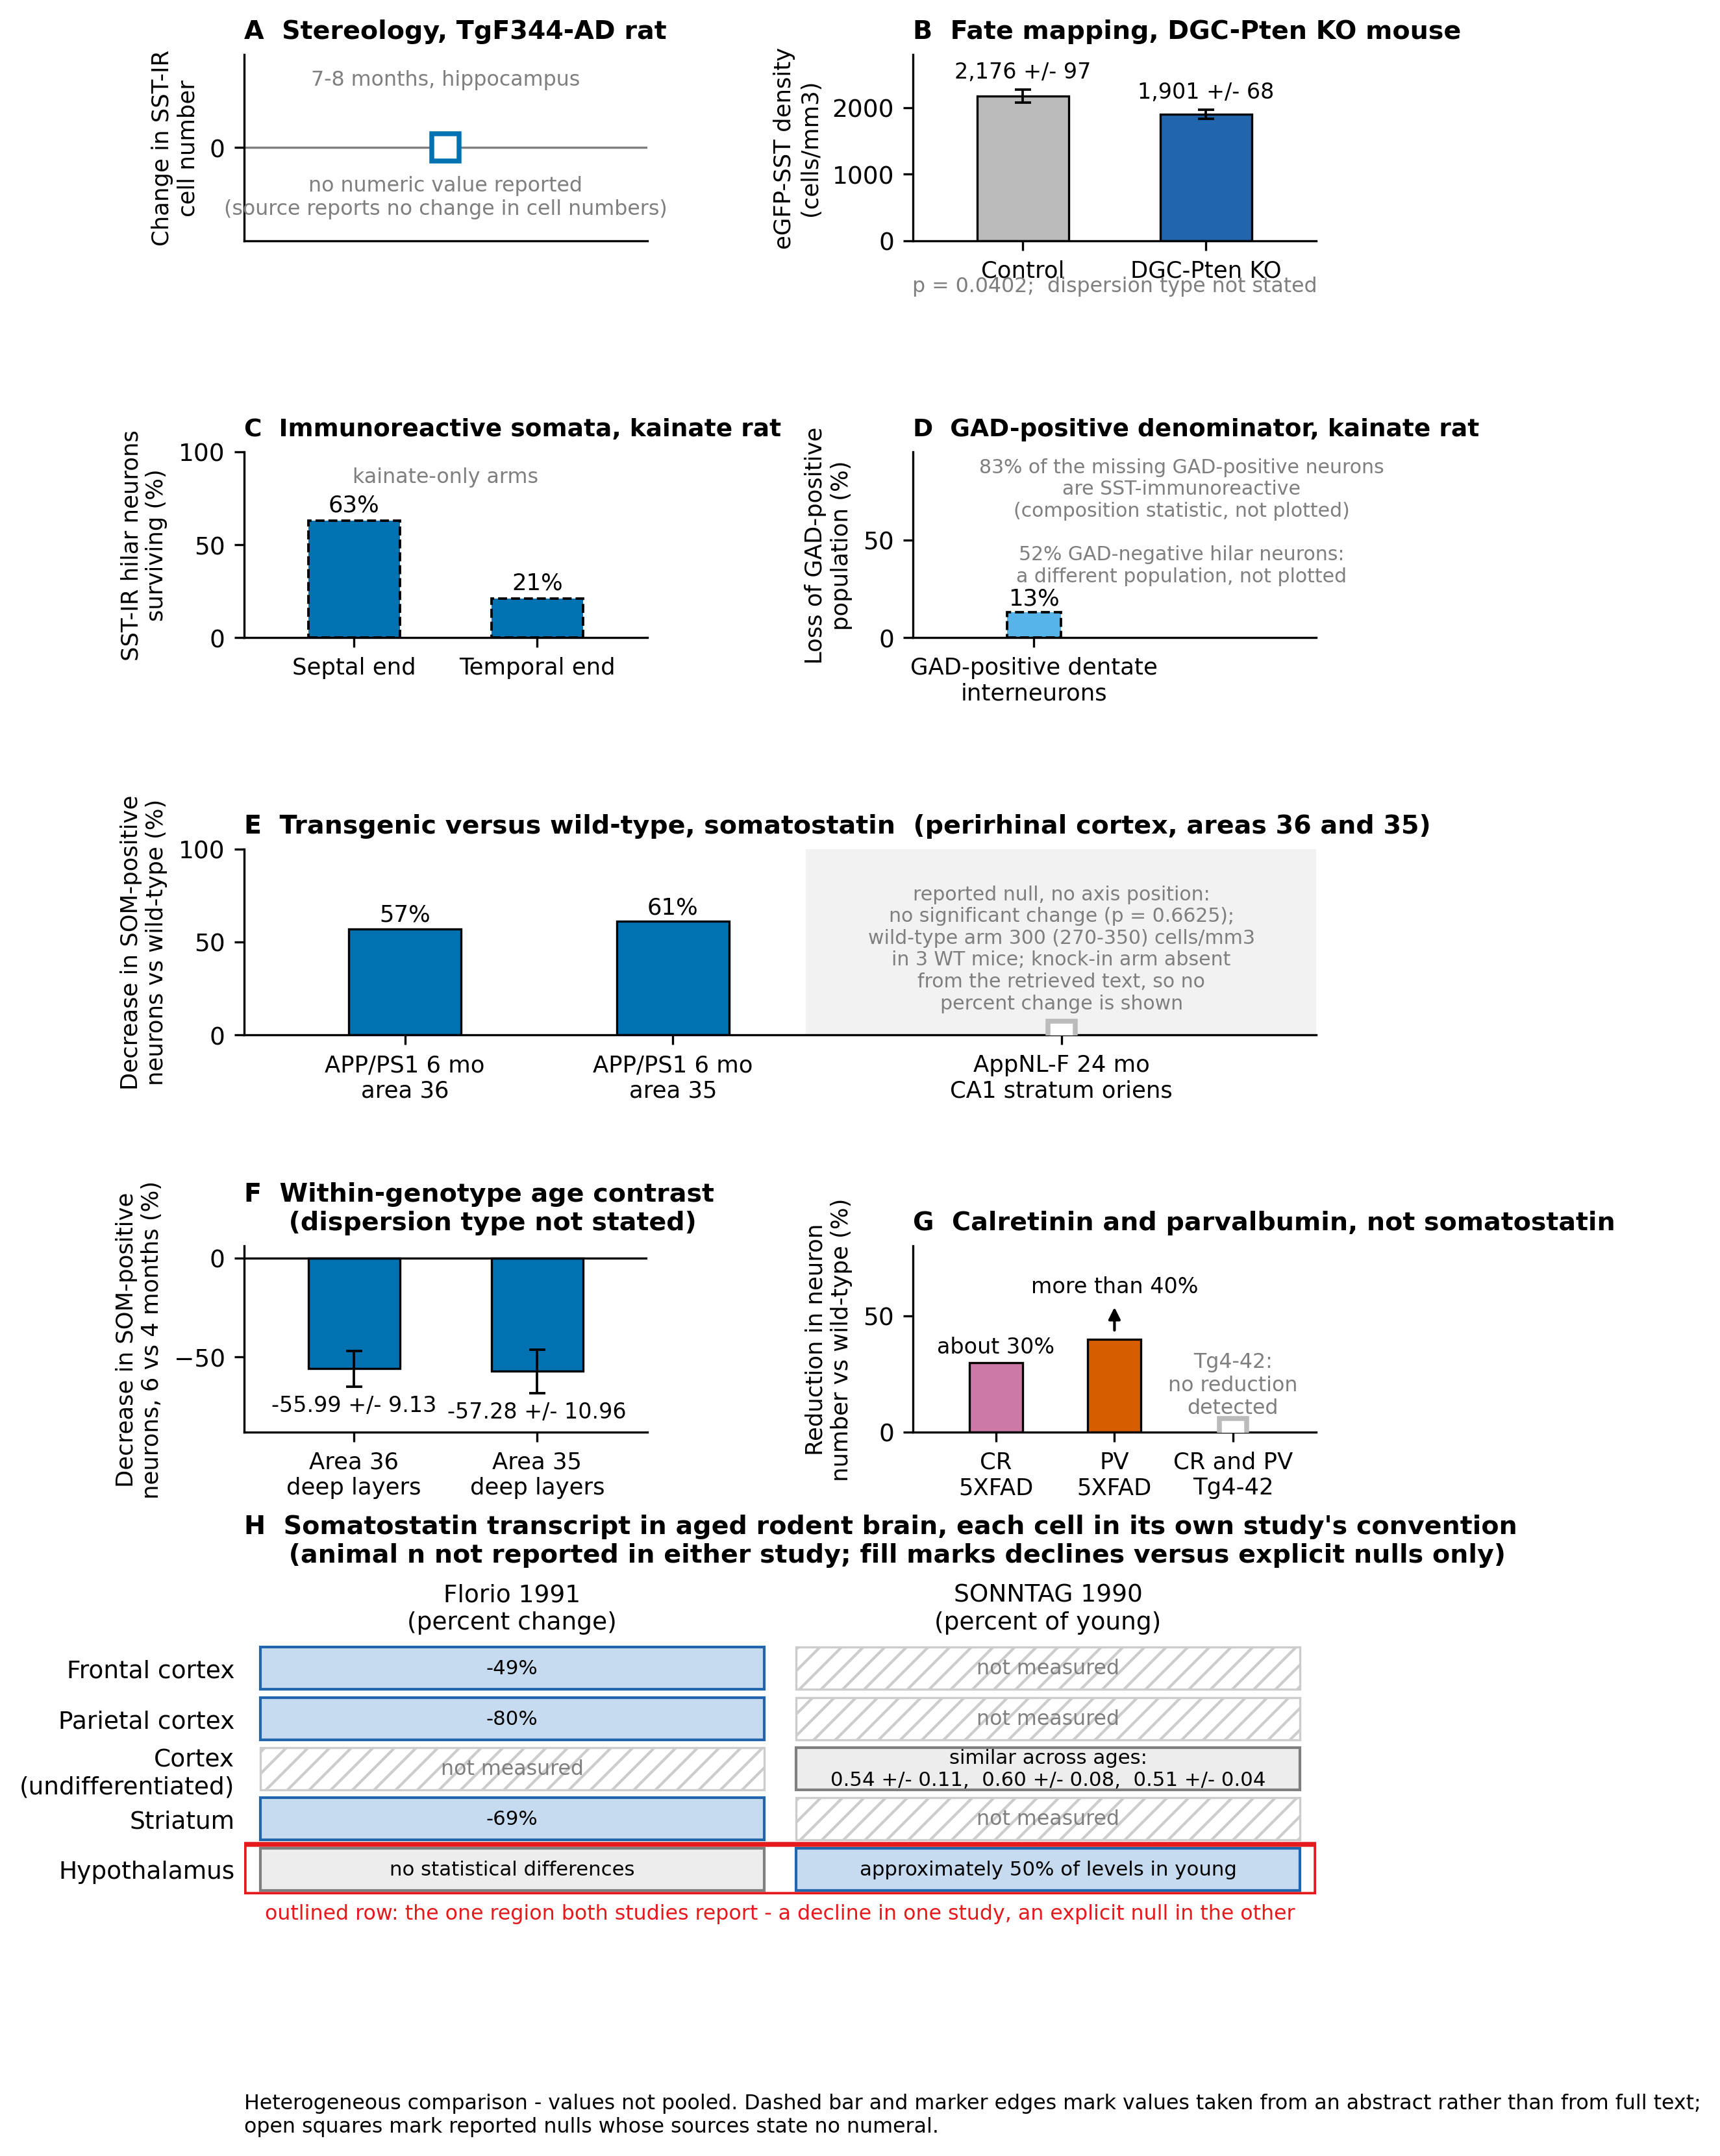
\includegraphics[width=\linewidth]{../figures/fig_sec11_measurement_determines_the_answer.png}
\caption{\textbf{Measurement strategy and reported somatostatin change.} Cell-count panels (A-D): design-based stereology in TgF344-AD rats (A), eGFP-SST fate-mapped density in DGC-Pten knockout mice (B), percent of somatostatin-immunoreactive hilar neurons surviving after kainate (C), and percent loss of the GAD-positive dentate population after kainate (D). Amyloid-model panels (E-G): somatostatin-positive neurons in transgenic versus wild-type mice (E), the within-genotype 6-month versus 4-month contrast (F), and calretinin- and parvalbumin-positive neurons in two models (G). Panel H is a region-by-study matrix of somatostatin transcript in aged rodent brain, printed in each study's own convention. Heterogeneous comparison - values not pooled. Entries are not a common measurement: cell number, cells/mm3 density, and percent survival are shown; values are not interconvertible and each panel carries its own axis. \citet{Buckmaster1999} quantify loss of all GAD-positive interneurons (13\%), not of somatostatin cells; 83\% of the missing GAD-positive neurons are somatostatin-immunoreactive, but that study reports no SST-specific loss percentage, and its 52\% figure is for GAD-negative hilar neurons (putative mossy cells), a different population, and is not plotted. \citet{Jolkkonen1997} is plotted as two values: 63\% surviving at the septal end and only 21\% surviving at the temporal end; both are the kainate-only arms, and the same study reports only 35\% of the neurons remaining in the septal end and 14\% in the temporal end when kainate is combined with cholinergic deafferentation, a different experimental condition that is not shown. Three distinct aetiologies (amyloid transgenic rat, Pten/mTOR genetic epilepsy mouse, kainate chemoconvulsant rat), two species and two detection modalities (eGFP fate-mapping versus peptide immunoreactivity) are represented, so apparent loss in the immunoreactivity entries may include marker downregulation. No animal n is stated in the retrieved sentences for any entry in panels A-D, and only \citet{Drake2024} carries an error term; no n is printed on any panel. \citet{Drake2024} is plotted as the two reported densities (2,176 and 1,901 cells/mm3), not as a derived percentage; its error terms are printed as the source prints them (+/- 97, +/- 68) and the source does not state whether the dispersion is SEM or SD; the same study reports expansion of the dentate molecular layer, so a cells/mm3 reduction in this model is not interchangeable with a cell-number reduction, and the somatostatin density reduction itself is reported for the hippocampus while the molecular-layer observation concerns the density of GFP+ processes. The proportion of dentate granule cells carrying the Pten deletion is not printed: the source states only that Pten is deleted from a subset of dentate granule cells. The TgF344-AD entry is drawn as a null marker without an error bar: its source reports no change and states no numeral. \citet{Giesers2020} reports calretinin- and parvalbumin-positive interneurons, not somatostatin; no somatostatin population is quantified in the retrieved text, and the study appears only in the separately titled non-SST panel G. Panel E states the quantity as the source does: \citet{SanchezMejias2019} reports a decrease in SOM-positive neurons of 57\% (area 36) and 61\% (area 35) in 6-month-old transgenic mice. This is not labelled a numerical density, because the retrieved text does not establish whether it is a count or a density, and the adjacent null is reported in cells/mm3; panel F states its quantity the same way, with the same limitation. \citet{Sos2020} is drawn as a null marker with no axis position and no error bar: its only reported figure is the wild-type arm, 300 (270-350) cells/mm3 in 3 WT mice, the knock-in arm is absent from the retrieved text, and no percent change may be inferred. Panel F dispersion is printed as reported (+/- 9.13\%, +/- 10.96\%); the source does not state whether it is SEM or SD. The panel E region is the perirhinal cortex, areas 36 and 35; the deep-layer restriction belongs to the 6-vs-4-month sentence and is printed only on panel F. The \citet{SanchezMejias2019} value in panel F is a 6-month vs 4-month within-genotype contrast; panel E carries only transgenic-vs-wild-type contrasts. Models, ages and regions differ (APP/PS1 at 6 months, perirhinal cortex; AppNL-F knock-in at 24 months, CA1 stratum oriens; 5XFAD and Tg4-42 at 12 months, hippocampal subfields), so construct class, age and region cannot be separated within this figure. The \citet{Giesers2020} reductions are subfield-specific - calretinin mainly in CA1 and CA2/3, parvalbumin in all analysed subfields including the dentate gyrus - not whole-hippocampus; the 5XFAD reduction (about 30\% calretinin, more than 40\% parvalbumin) and the Tg4-42 null are shown as separate bars from the same study, and the non-plaque-forming model showed no reduction. \citet{SanchezMejias2019} also reports a 91\% SOM decrease in Braak V-VI human cases; that human value is not on these axes. No animal n is stated in the retrieved sentences for the \citet{SanchezMejias2019} or \citet{Giesers2020} entries. In panel H the two studies disagree where they overlap: \citet{Florio1991} reports no change in hypothalamus, \citet{SONNTAG1990} reports no change in cortex; both nulls are shown. Both are bulk-tissue mRNA measurements, and the in situ analysis of \citet{SONNTAG1990} attributes its hypothalamic decrease to decreased expression within specific hypothalamic nuclei rather than a loss of somatostatin-containing neurons. Animal n is not stated in either source and neither states its unit of replication; the controls differ - \citet{Florio1991} reports its reduction as occurring despite no change in beta-actin gene expression, while \citet{SONNTAG1990} expresses somatostatin mRNA relative to poly A+ RNA. Values are expressed on different conventions (percent change for \citet{Florio1991}, percent of young levels for \citet{SONNTAG1990}); they are printed in their own conventions and are not converted, the matrix has no bars and no shared numeric axis, fill distinguishes declines from explicit nulls only, and the printed cell text carries the magnitude in each study's own convention. The cortical sample of \citet{SONNTAG1990} is undifferentiated whereas \citet{Florio1991} reports named areas (frontal -49\%, parietal -80\%), so part of the cortical disagreement may reflect dissection grain rather than a contradiction, since a pooled cortical sample can dilute an area-specific decline.}
\label{fig-sec11-measurement-determines-the-answer}
\end{figure}

\subsection{Genetic access is neither complete nor specific}
\label{sec-11-genetic-access}

The fate-mapping argument that separates marker downregulation from cell death is only as good as the driver line carrying it, and the error runs in both directions, as \ref{fig-sec11-genetic-label-fidelity} shows. In situ hybridisation against Sst mRNA in SST-IRES-Cre;tdTomato hippocampus found only 48/127 (37.8\%) reporter-positive cells in the CA3 pyramidal cell layer to be Sst-expressing, against 82/100 (82\%) in stratum oriens and 61/74 (82.4\%) in stratum radiatum - specificity that is lamina-dependent within one subfield \citep{MullerKomorowska2020}. In presubiculum, somatostatin immunolabelling identified 89\% of fluorescent cells in the X98 line but 71\% in Sst-Cre animals, and 6 $\pm$ 3\% of labelled neurons expressed both parvalbumin and somatostatin, so the marker categories overlap inside the labelled population; the authors attribute the lesser specificity of the Sst-Cre line to off-target recombination, possibly linked to maternal cre inheritance, and the retrieved text does not say what accounts for the somatostatin-negative remainder \citep{Nassar2015}. The converse failure is as large: a GFP line long used as a proxy for cortical somatostatin interneurons labels 44\% of the somatostatin-positive population in layer II/III and around 35\% in layers IV and Va, with 29\% of labelled cells co-expressing calretinin \citep{Zhou2019}, so physiology from that line describes a biased subset. The same classes of failure are documented beyond these lines. reports that Cx3cr1-Cre microglial drivers label scattered non-target neurons brain-wide differ between nominally equivalent lines and between studies, and the study that tested two such lines directly found reporter expression largely restricted to microglia, attributing the neuronal labelling other groups reported to Cre-independent reporter leakiness \citep{Zhao2019}; drivers nominally targeting one population differ in the spatiotemporal pattern of recombinase activity, which their authors argue would itself produce divergent phenotypes from one floxed allele \citep{Zhou2021}; interneuron driver strains including Sst-Cre are maintained on a background carrying an age-related hearing-loss allele, so sensory decline confounds the ageing phenotypes they are used to study, a confound reported in an unrefereed preprint \citep{Foss2024}; a further marker, glutaminyl cyclase, is expressed across subsets of five interneuron marker classes, so marker categories are not nested cleanly \citep{HartlageRubsamen2009}; and in a systematic test of commercial receptor antibodies, no proposed antibody-validity criterion other than the knockout control established specificity for brain immunohistochemistry \citep{Baek2013}. The figures quantified in \ref{sec-sst-identity} therefore bound every rodent count here that is made through a driver line; the immunoreactivity counts carry the separate error of marker downregulation. Two gaps follow: no systematic region-by-region and age-by-age audit of Sst-Cre fidelity was retrieved by these searches, and no study re-measuring reporter specificity or coverage under amyloid, tau or polyglutamine pathology was retrieved at all - so the control is circular where it is most load-bearing, since if Sst transcription falls in disease, recombination history and current marker status diverge.

\begin{figure}[H]
\centering
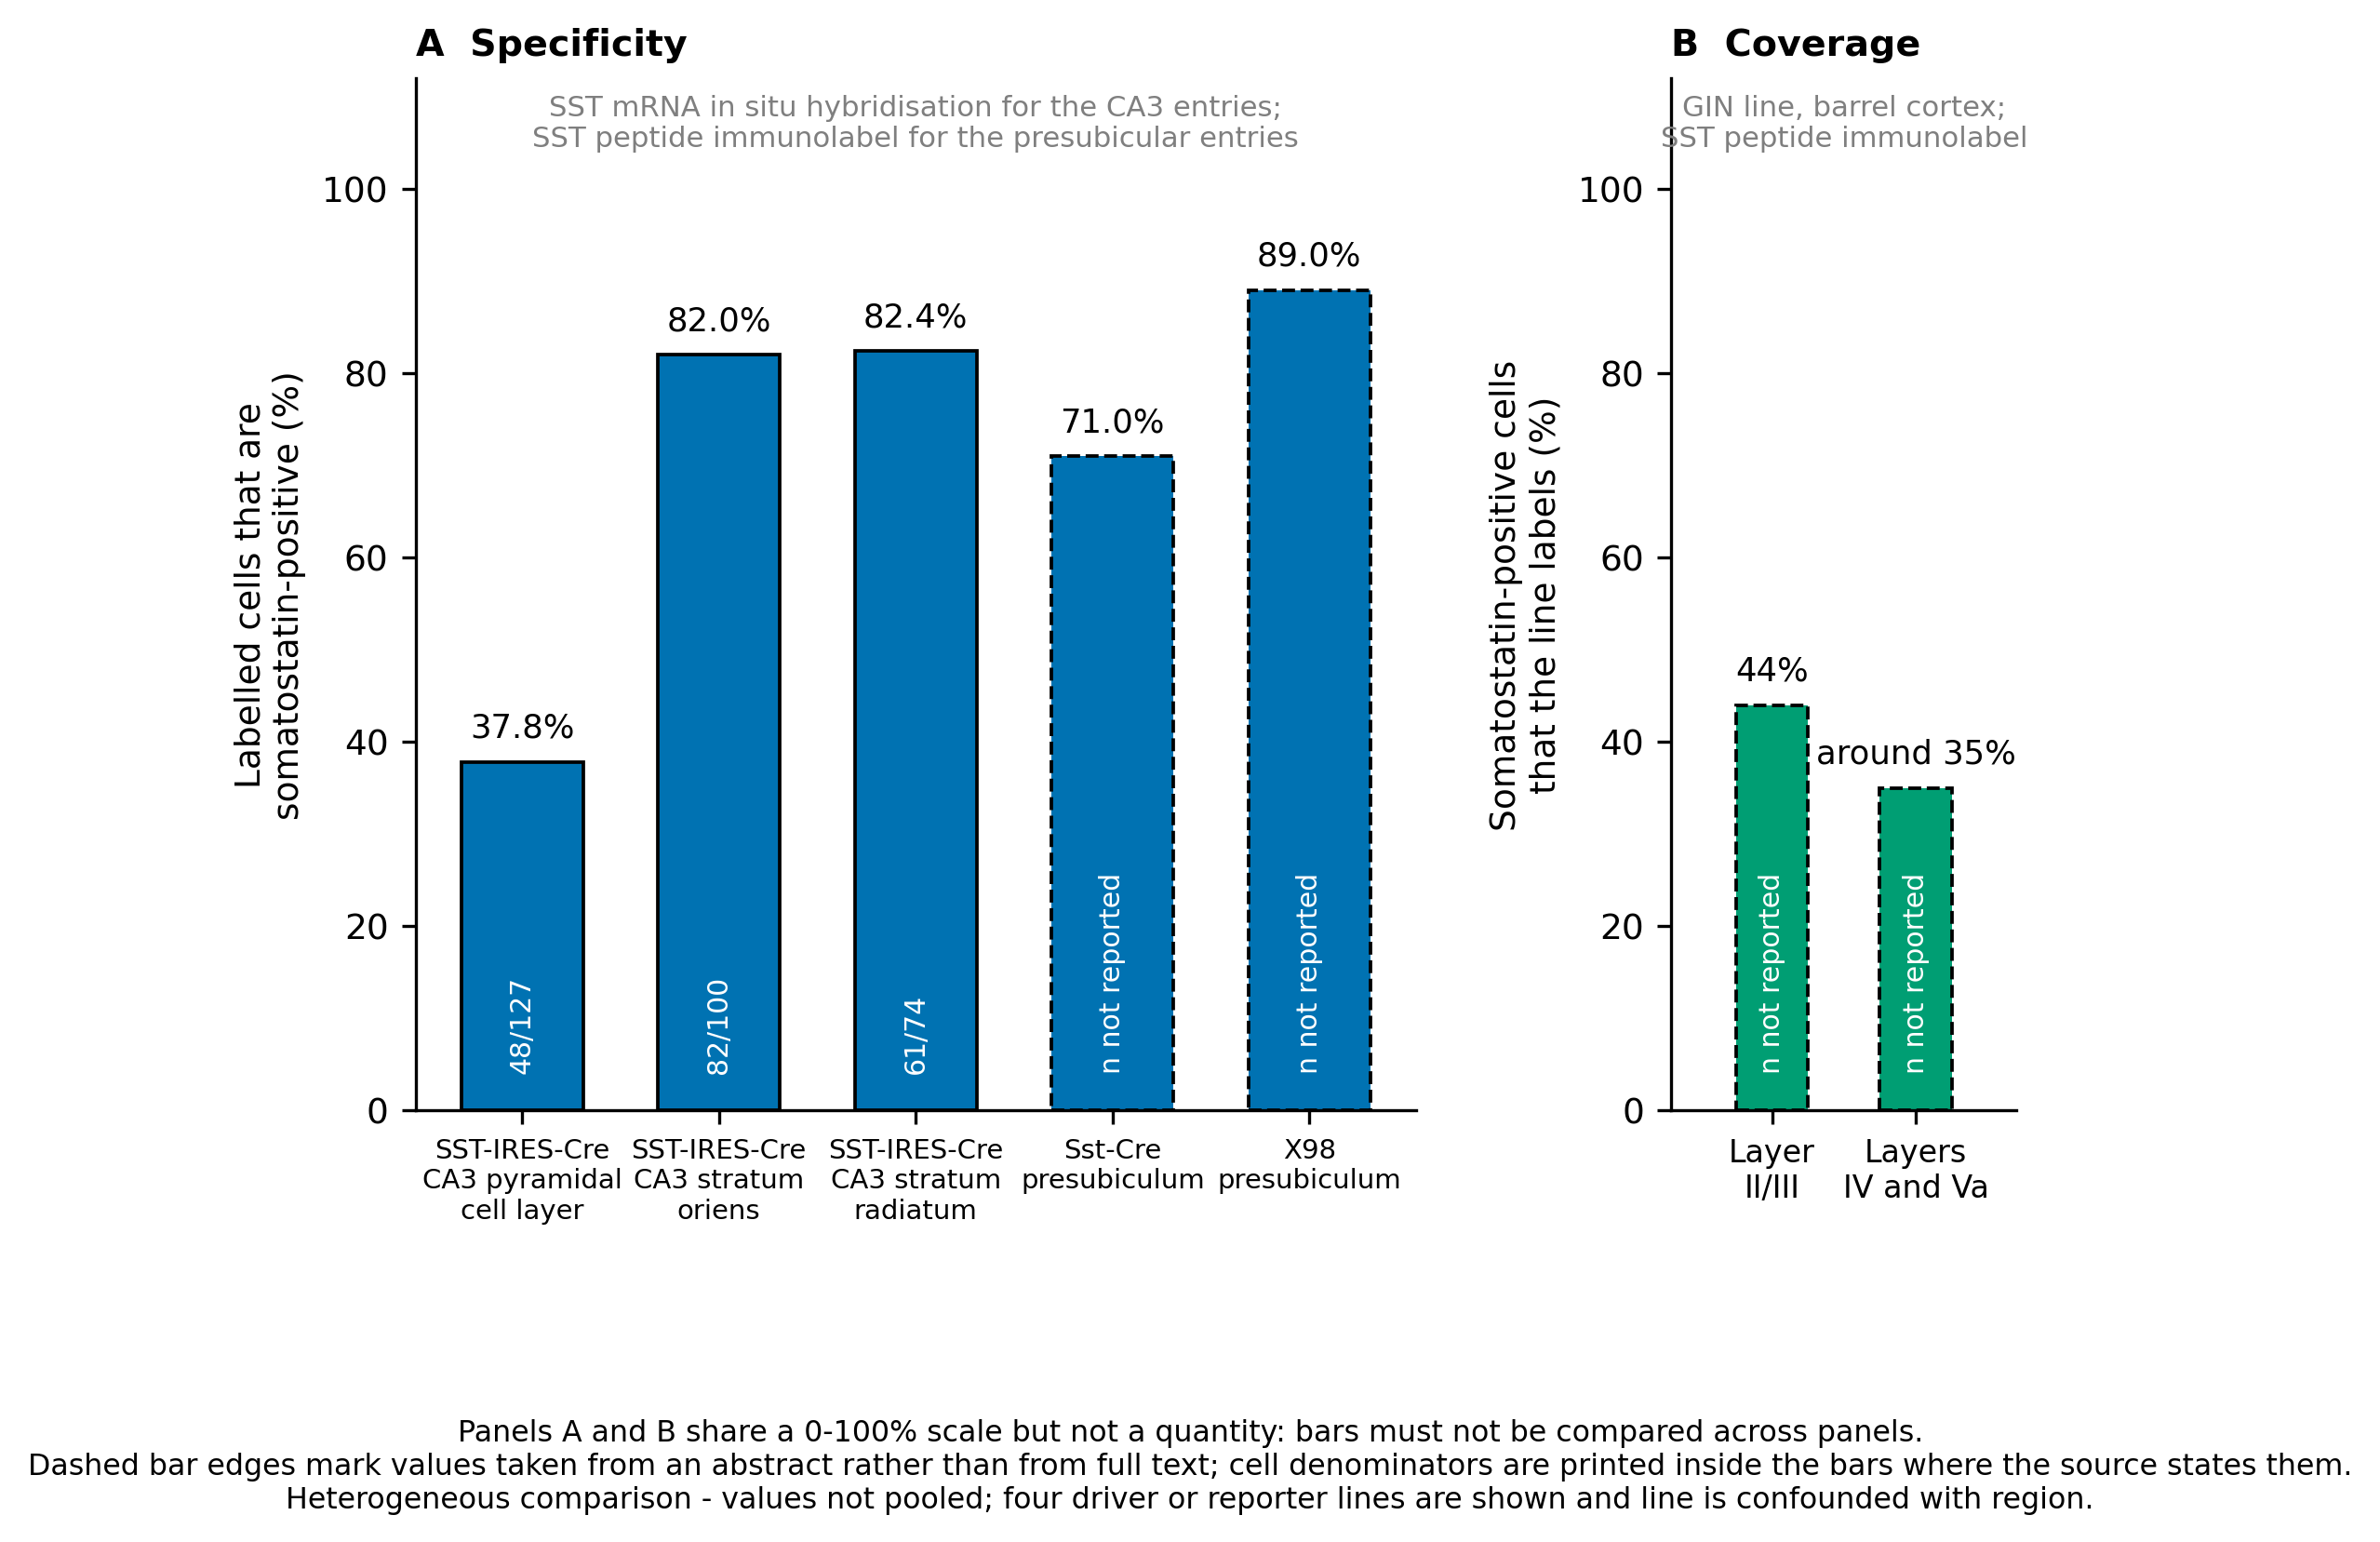
\includegraphics[width=\linewidth]{../figures/fig_sec11_genetic_label_fidelity.png}
\caption{\textbf{Genetic labelling versus somatostatin marker expression across mouse lines.} Panel A, specificity: percent of labelled cells that are somatostatin-positive. Panel B, coverage: percent of somatostatin-positive cells that the line labels. Heterogeneous comparison - values not pooled. Panels A and B share a 0-100\% scale but not a quantity, and bars must not be compared across panels: specificity and coverage are opposite failures of genetic access, so a low specificity and a low coverage do not mean the same thing. The two panel A lines are different lines from different studies measured by different methods and are not two measurements of one line: SST-IRES-Cre as measured by \citet{MullerKomorowska2020} in CA3 with SST mRNA in situ hybridisation, and Sst-Cre as measured by \citet{Nassar2015} in presubiculum with SST peptide immunolabel. The 37.8\% for SST-IRES-Cre is the CA3 pyramidal cell layer only; the same sentence reports 82\% in stratum oriens and 82.4\% in stratum radiatum. Detection differs: SST mRNA in situ hybridisation in \citet{MullerKomorowska2020} versus SST peptide immunolabelling in \citet{Nassar2015} and \citet{Zhou2019}; that immunolabel-based specificity is therefore a lower bound is an inference about detection methods, since peptide immunoreactivity can be below detection in cells transcribing Sst, and is not a finding of either study. Denominators are reported only for \citet{MullerKomorowska2020} (48/127, 82/100, 61/74); the presubicular and barrel-cortex entries do not state how many cells were scored, so no intervals are drawn. \citet{Nassar2015} reports that 6 $\pm$ 3\% of labelled neurons in Sst-Cre presubiculum expressed both parvalbumin and somatostatin; those cells are somatostatin-immunopositive and therefore fall inside the 71\% specificity value rather than in the shortfall from 100\%, which the retrieved text does not account for; the Sst-Cre shortfall is attributed by those authors to off-target recombination possibly linked to maternal cre inheritance, a mechanism that does not generalise to the other lines. The \citet{Nassar2015} values are two separate mouse lines (Sst-Cre 71\%, X98 89\%) and are plotted as separate bars. Regions differ (hippocampal CA3 laminae, presubiculum, barrel cortex layers II/III-Va) and line is confounded with region. Marker edges are dashed where the value comes from an abstract rather than full text.}
\label{fig-sec11-genetic-label-fidelity}
\end{figure}

\subsection{Construct and dosage as a predictor of phenotype}
\label{sec-11-construct-dosage}

In the material retrieved here, reported interneuron phenotypes sort more consistently by model class than by pathology, although no study compares the two directly, and the proximate candidate is dosage, as set out in \ref{fig-sec11-model-construct-and-transgene-dosage}. A knock-in line showed similar full-length APP in knock-in and background-strain cortex at 3, 6 and 9 months, confirming physiological expression \citep{Yeapuri2025}; a genomic human MAPT transgene under its native promoter produced less than a 35\% increase over endogenous mouse tau \citep{Guo2013}; and a widely used tauopathy line is described in the review literature as carrying P301L tau at about 13 times endogenous levels, reducible to about 3 times with doxycycline, a reduction that reversed behavioural impairment while neurofibrillary tangles continued to accumulate \citep{Sahara2023}. Transgene integration in such lines also disrupts endogenous genes at the insertion site, which is why the field has been urged to sequence every overexpression line in use before its phenotypes are read as amyloid effects \citep{Sasaguri2022}. Overexpression further distorts the protein's cellular distribution, since endogenous APP is enriched in GABAergic interneurons rather than uniformly expressed \citep{Rice2020}, and conclusions about amyloid modifiers rest almost entirely on lines whose non-physiological promoters make APP processing unlike the human situation \citep{Xie2021,SchedinWeiss2020}; where and when the transgene is active matters as much as how much of it there is, since adult-onset human APP expression produces region-specific rather than uniform hyperexcitability \citep{Goettemoeller2024}.

The behavioural phenotype against which interneuron changes are usually interpreted inherits the same instability, and whether App knock-in mice develop behavioural and glial phenotypes at all is itself disputed and unresolved: one series reports negligible cognitive, locomotor and microglial change in AppNL/NL mice despite increased insoluble amyloid-beta \citep{Salas2018}, while the opposing report describes cognitive and emotional alterations in App knock-in mice and argues that APP overexpression produces memory impairment without amyloid deposition in some lines \citep{Sakakibara2018}. Allele number (NL versus NL-G-F), age and test battery differ between them, the sentence recorded for the second study speaks to overexpressing rather than knock-in lines, and no arbitrating study was retrieved by these searches. A Y-maze deficit reported in one laboratory was absent in another \citep{Jacob2019}; one knock-in line gave opposite anxiety readings in two tasks run on the same animals \citep{Pervolaraki2019}; and strain background sets the baseline against which all of this is measured, documented not as a behavioural baseline but as strain-dependent striatal and nigral interneuron protein levels in relation to MPTP susceptibility \citep{Bhaduri2018}; and the absence of overt degeneration in knock-in mice is partly a species limitation, since an App knock-in rat lost 9.11\% of brain weight by 12 months and 16.09\% by 22 months \citep{Pang2021}. Construct-specific limitations of the same kind are documented for every existing TDP-43 nuclear-localisation-signal model \citep{Mitra2025}. No multi-site or pre-registered replication of App knock-in cognitive phenotypes was retrieved by these searches, and no study counting somatostatin interneurons in an overexpression line and a knock-in line side by side with one protocol, one age series and one observer was retrieved either - so the central model-validity claim of this literature, that interneuron depletion is an overexpression artifact, rests on exactly the cross-study inference that the counting-variance literature says is unreliable.

\begin{figure}[H]
\centering
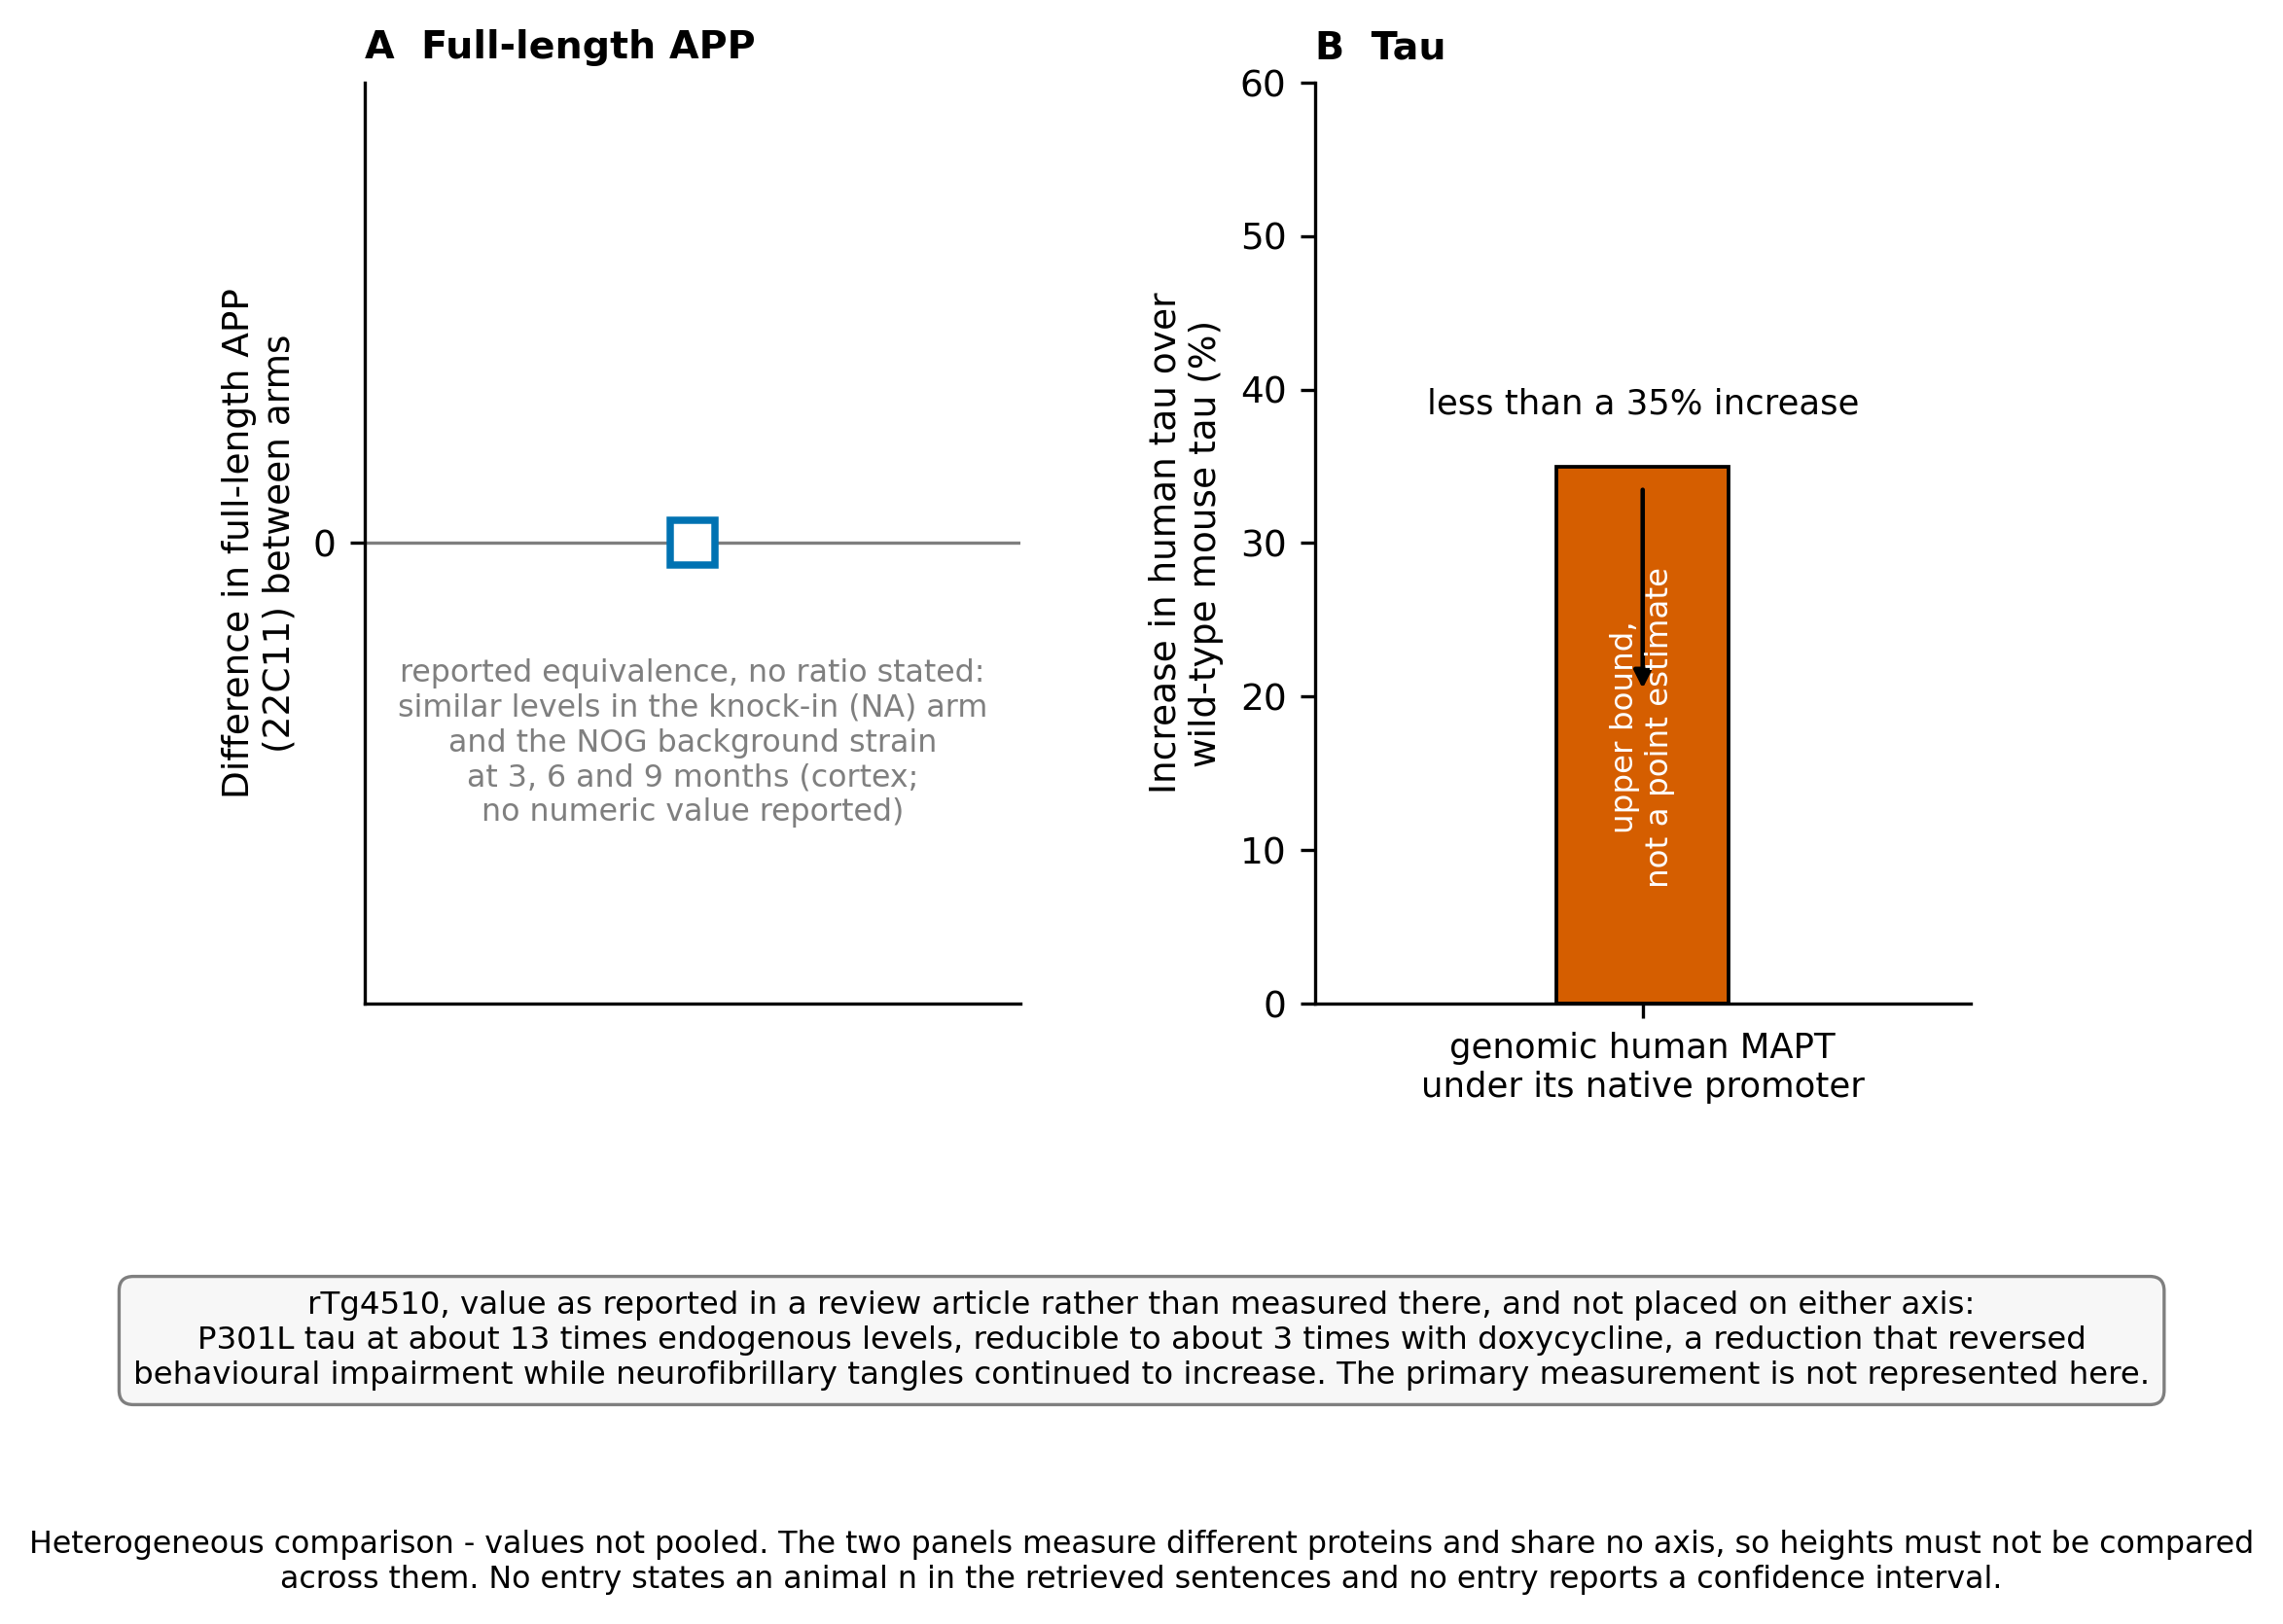
\includegraphics[width=\linewidth]{../figures/fig_sec11_model_construct_and_transgene_dosage.png}
\caption{\textbf{Transgene expression relative to endogenous protein across Alzheimer and tauopathy model classes.} Panel A, full-length APP; panel B, tau. Heterogeneous comparison - values not pooled. Measurements are of different proteins (full-length APP; human tau; P301L tau); fold over endogenous is a shared unit, not a shared quantity, and the two panels share no axis, so bar heights must not be compared across them. \citet{Yeapuri2025} reports similar full-length APP levels in the knock-in and background-strain mice (a reported equivalence, no ratio stated), and the panel A contrast is the single knock-in arm (NA) against the NOG background strain on which the knock-in was made - not a conventional wild-type, and not the double APP plus PS1 knock-in that the same abstract reports as doubling the amyloid load. \citet{Guo2013} reports less than a 35\% increase of human tau over wild-type mouse tau, an upper bound rather than a point estimate, drawn as a bound on a percent-increase axis; neither entry is a measured ratio and neither carries a confidence interval. The rTg4510 value (about 13 times endogenous levels, reducible to about 3 times with doxycycline) is quoted from a review article rather than measured there \citep{Sahara2023}; it is shown as a labelled annotation set clear of the panel B axis, with no axis position, and the primary measurement is not represented in the material retrieved here. Transgene scope differs where it is stated: an endogenous APP locus knock-in \citep{Yeapuri2025} and a genomic human MAPT transgene under its native promoter \citep{Guo2013}. The rTg4510 transgene's scope is not stated in the retrieved text, and no claim is made here about which cells carry its dose. No entry states an animal n in the retrieved sentences, and no entry reports a confidence interval. The tissue of measurement for \citet{Guo2013} is not stated in the retrieved text.}
\label{fig-sec11-model-construct-and-transgene-dosage}
\end{figure}

\subsection{Human tissue confounds and cross-species transfer}
\label{sec-11-human-tissue}

On the human side the first confound is that tissue quality is not a nuisance variable but a measured effect. A 3 h postmortem interval alone generated 79 upregulated and 53 downregulated neuronal differentially expressed genes and obscured genotype effects in a tauopathy line \citep{Olney2025}; in human brain banks, 96\% of samples from autopsies under five hours reached an RNA integrity number of 7.5 or more against 74\% from longer intervals \citep{Birdsill2010}; brain pH was lower in Alzheimer cases than controls (6.4 versus 6.5) and correlated positively with measurable mRNA for every gene examined except GFAP \citep{Preece2003}; and pH and RNA integrity each exerted gene-set-specific effects in a 13-brain schizophrenia microarray series that the cited study summarises from its authors' own earlier work, the cited study itself covering 25 schizophrenia, 10 bipolar and 21 control brains, so unadjusted comparisons confound disease signal with tissue state \citep{Hatano2025}. Whether those confounds act uniformly is disputed: RNA integrity varied with both diagnosis (p = 0.0350) and region (p = 0.0142) in Alzheimer's disease but not in Huntington's or Parkinson's disease \citep{Highet2021}, implying diagnosis-dependent confounding that no single covariate removes, whereas the pH-expression correlations were reported to hold consistently across all groupings of pathology and sex \citep{Preece2003}, which would make the confound uniformly correctable. The two have not been reconciled. The question is sharpest for somatostatin, because neuropeptides degrade rapidly after death unless enzymes are inactivated by in vivo heat stabilisation \citep{Salviati2025} - a control unavailable in autopsy material - and because pH and lactate shifts also occur in unmedicated mouse models, so they are not purely agonal artefacts \citep{Hagihara2017}. No dose-response curve for somatostatin peptide or Sst transcript against postmortem interval, brain pH or agonal duration in human tissue was retrieved by these searches, so the reported human deficits can be neither corrected nor bounded.

Cohort composition and the choice of statistical unit compound the problem. In an autopsy series of rapidly progressive dementia, concomitant pathologies were present in 117 of 160 cases (73\%) and clinicopathological agreement outside prion disease was 21\% against 94\% within it \citep{GrauRivera2015}; white matter interstitial neurons have been quantified in only a handful of whole-brain series \citep{Zouridakis2023}, and fall outside cortical counts as those are conventionally bounded; and in a postmortem schizophrenia cohort a composite index summing GAD67 and SST mRNA alterations was lower in 80.4\% of cases and was associated with final educational attainment (adjusted odds ratio 1.44, p = 0.022) \citep{Dienel2025} - the analytic unit partly determines what a postmortem comparison reports. Against that background, the human marker-count evidence for preferential somatostatin vulnerability - p = 0.0001 for somatostatin and p = 0.013 for calretinin cells colocalising with amyloid-beta in piriform cortex, with parvalbumin prevalence increased \citep{SaizSanchez2014}, and a model counterpart in which somatostatin cells colocalise heavily with amyloid in olfactory cortex \citep{SaizSanchez2012} - stands in unresolved tension with direct peptidomic measurement in pathology-matched cases, where SST-14 is maintained in the resilient brain despite amyloid burden \citep{Morgan2024a}, a cohort argued at length in \ref{sec-alzheimers}. The two sides differ in modality, immunoreactive cell counts against peptide quantification, and in how the cohort was stratified, by diagnosis against cognition at matched pathology; neither measurement adjudicates the other. Cortical peptide change in Huntington's disease runs the other way, with somatostatin increased in a minority of areas, cholecystokinin elevated 57-153\%, and no cortical peptide change in rats given striatal lesions \citep{Mazurek1997}, which is why the comorbidity and region arguments of \ref{sec-parkinsons-lewy-body} and \ref{sec-huntingtons} cannot be collapsed into one disease effect; the marker-versus-cell disagreements recorded for prion disease, traumatic injury and Down syndrome in \ref{sec-als-ftd} are external replications of the same problem.

Cross-species transfer fails or holds depending on the level of description, and the two findings usually cited against each other are not in fact incompatible. Transcriptomic matching across mouse, marmoset and human motor cortex placed closely related types, among them Sncg and somatostatin subtypes, at chance-level correspondence (mean AUROC 0.50 across species against 0.84 within), while distinct types such as chandelier and Sst Chodl matched well \citep{Bakken2021}; human and mouse cortex differ in interneuron class proportions (50.2 $\pm$ 2.3\% versus 67.8 $\pm$ 0.9\% medial-ganglionic-eminence-derived) and 18\% of genes in the Sst Chodl type diverge more than tenfold \citep{Hodge2019}; cross-species integration requires an investigator-supplied homology mapping and identifies at least one mouse inhibitory class not detected in human data \citep{Liu2022}; and marker-defined interneuron categories differ in relative abundance between species, with calretinin rather than parvalbumin cells predominating in the claustrum of human and chimpanzee while parvalbumin density slightly exceeded calretinin in the one monkey examined \citep{Pirone2014}. Yet proportional changes in input excitability during membrane hyperpolarisation are conserved between human and mouse parvalbumin interneurons despite species differences in absolute input resistance \citep{Furdan2026}, and the generalised assumption that all GABAergic subclasses share a dependence on a single channel fails within mouse itself \citep{Liebergall2024}. Subtype identity is the level at which mouse data do not transfer; intrinsic biophysical mechanism is a level at which they may. Human-cell systems that bypass the inference are now available - grafted human pluripotent-stem-cell-derived medial ganglionic eminence cells develop almost exclusively (97\%) into SST and PVALB subtypes \citep{Bershteyn2025} - and early functional phenotypes in humanised knock-in models are measurable before any cell loss, with entorhinal parvalbumin interneurons hypoexcitable while neighbouring excitatory neurons are hyperexcitable at two months \citep{Gonzalez2026}.

\subsection{An inventory of the disagreements}
\label{sec-11-inventory}

Ninety cross-study disagreements were recorded across the ten topic areas of this review, and \ref{fig-sec11-conflict-atlas} classifies all of them by the axis on which the two studies differ and by status. Measurement modality and what was counted is the largest primary axis (37 of 90), followed by species, region and circuit context (21), model construct and species transfer (17), cohort composition, stage and comorbidity (8), and design rigor and statistical unit (7); 77 of the 90 span more than one axis, so the primary assignment marks emphasis rather than a partition. Forty-five are open and eleven unresolved, against twenty-three resolved by identifying the methodological difference and eleven partially resolved - which is what justifies treating the axes, rather than the diseases, as the organising variables. The last axis is the one least often visible in primary reports: neuron-number estimates for the same structure differ by about 15\% between groups using the isotropic fractionator and often differ by more than 100\% when the same stereological method is applied by different investigators to the same species and structure \citep{HerculanoHouzel2015}; frozen sections shrink along the z-axis to roughly 25\% of cut thickness with about 10\% between-section variability, biasing optical-disector counts unless measured thickness is used \citep{Carlo2011}; automatic image alignment in a physical-disector implementation gives a considerable economy of effort over manual alignment of tissue sections \citep{Fabricius2017}; and between-animal variance accounted for 31.98\% and 52.83\% of total variance in excitatory and inhibitory synaptic charge, so small-cohort studies can report group differences that reflect animal sampling \citep{Chen2018}. Two limits on the inventory must be stated plainly. The searches for disconfirming evidence were capped per query, so the inventory is a top-relevance sample rather than a census and the number of contradicted or unreplicated claims is bounded below, not estimated. The evidence behind this section is also unevenly verified: 45 of the 79 papers in its source literature were available as full text, and 25 of the 60 findings used here are recorded at abstract level only - a shortfall that is not confined to the older closed-access literature, since ten of those abstract-only records were published from 2018 onward and their quantitative claims could not be checked against a full text. The human cortical Huntington estimate discussed in \ref{sec-huntingtons} is an unrefereed preprint, treated as provisional wherever it appears.

\begin{figure}[H]
\centering
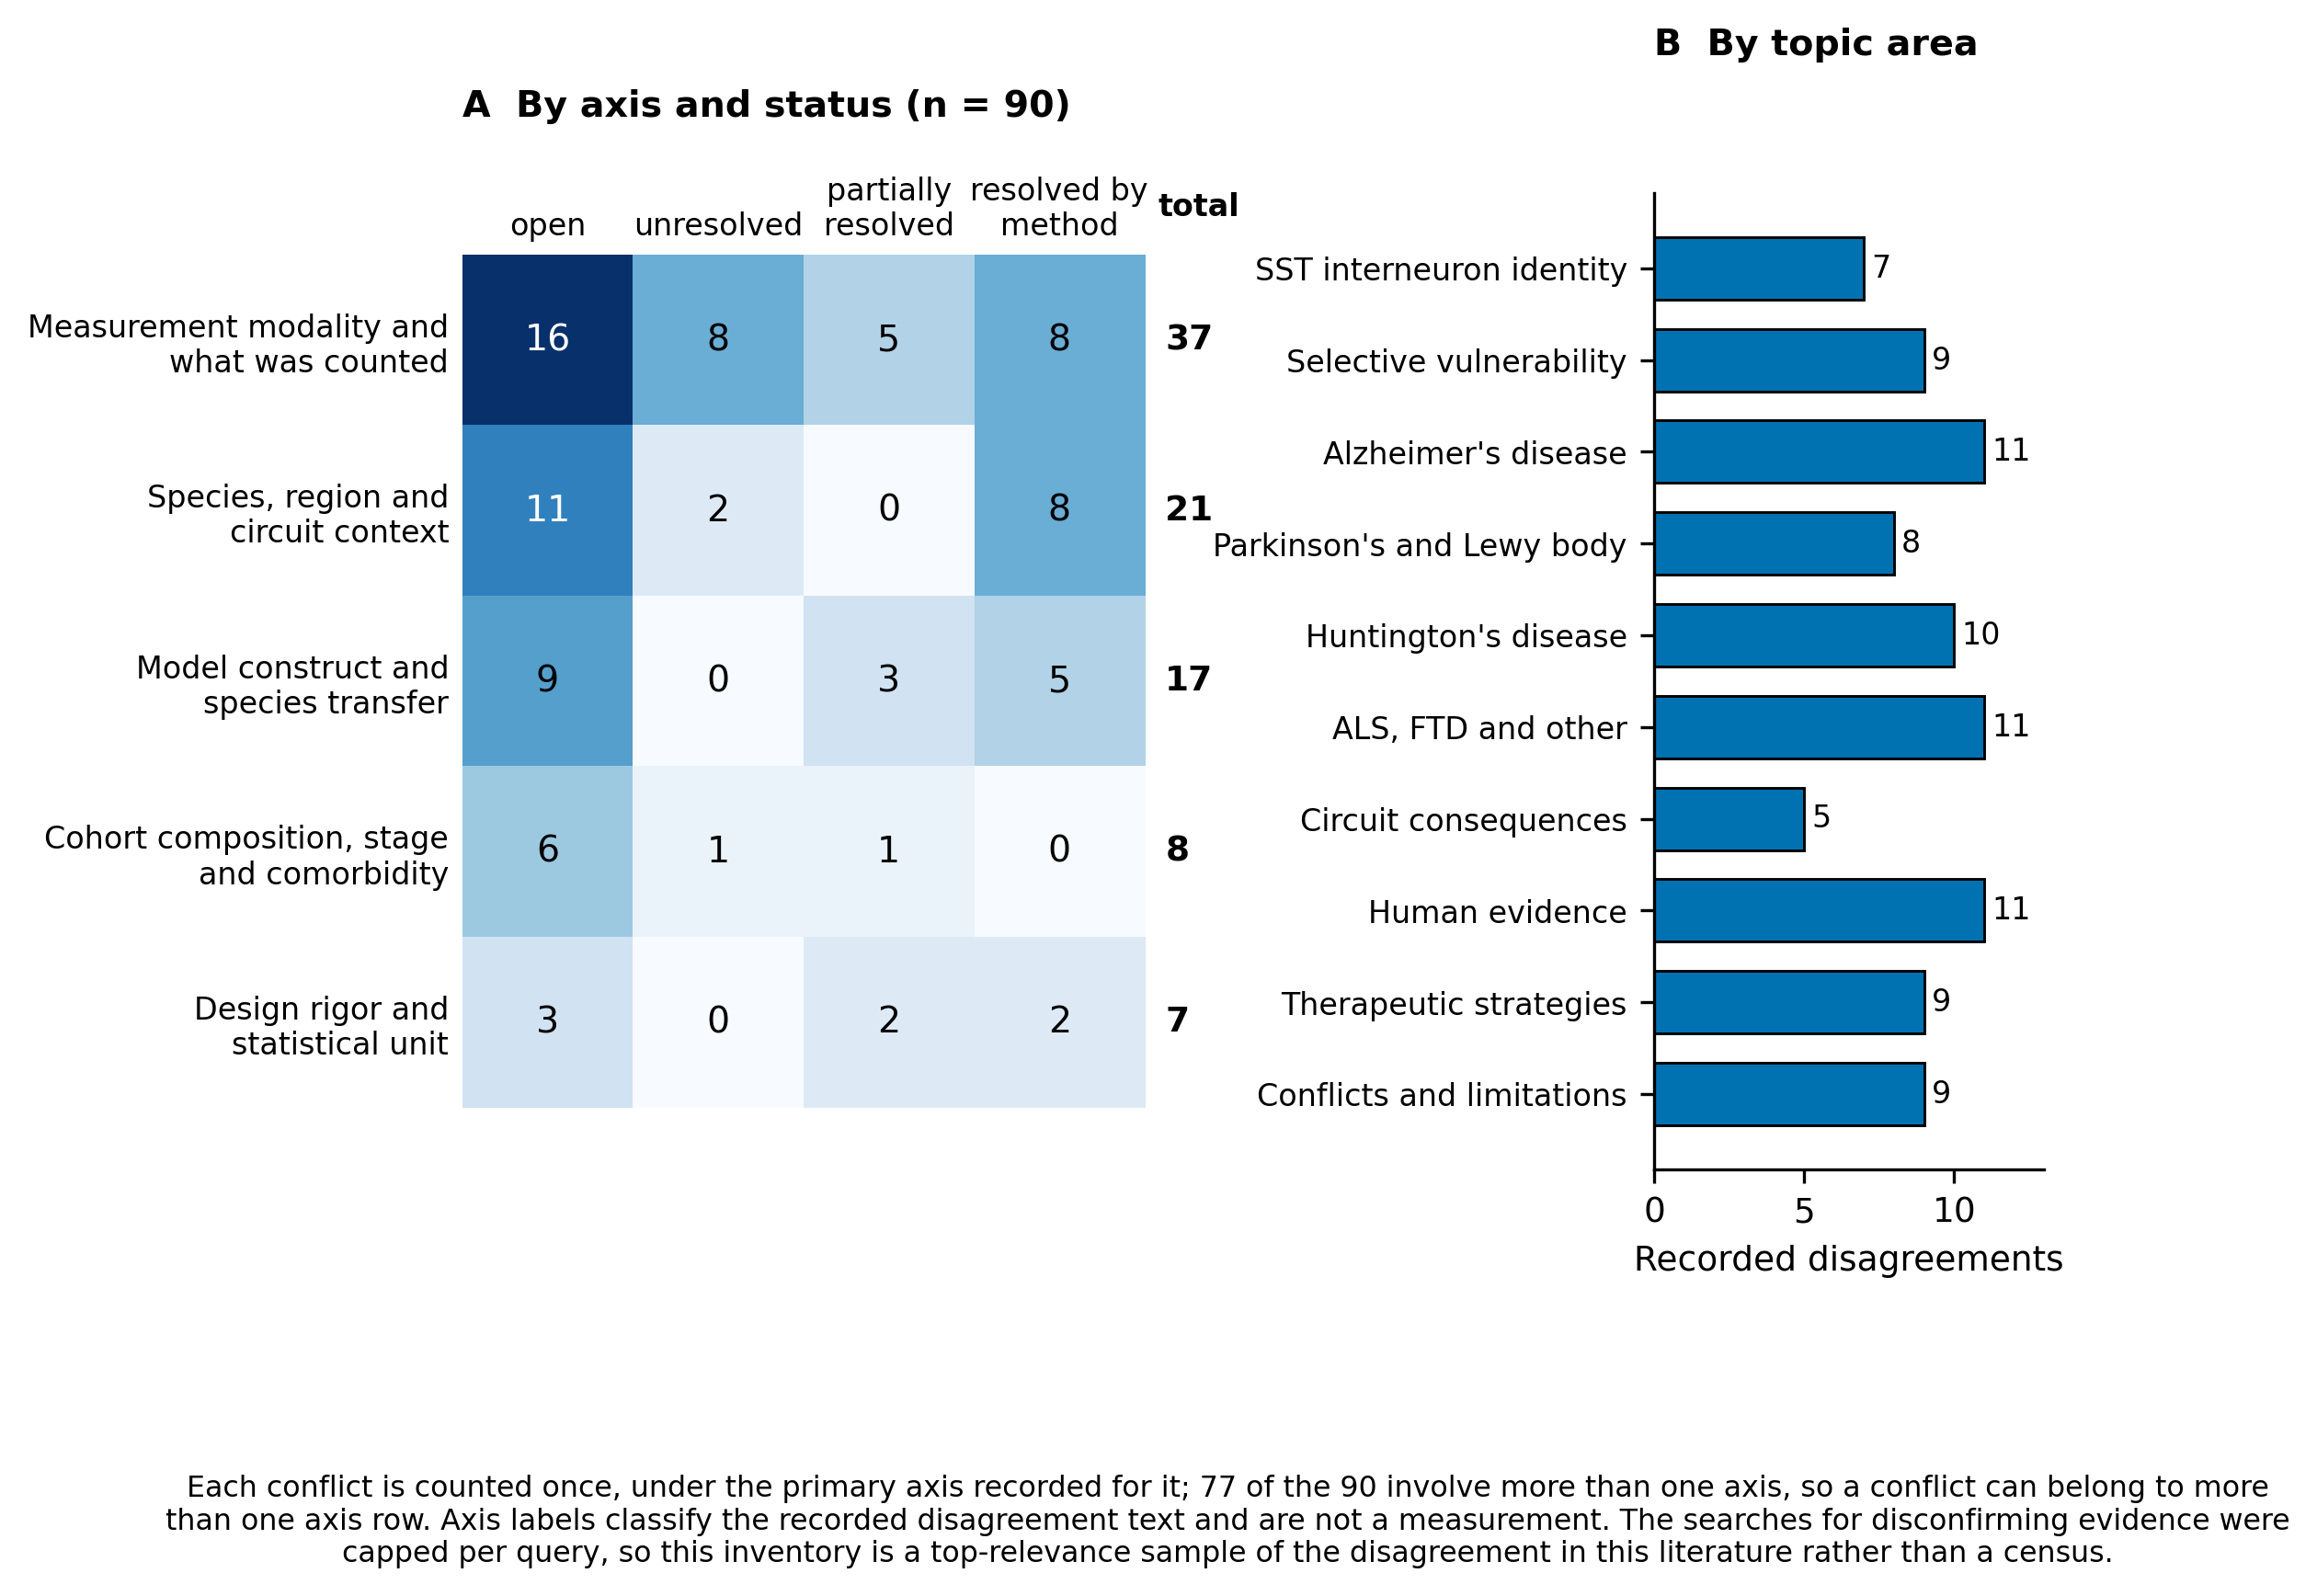
\includegraphics[width=\linewidth]{../figures/fig_sec11_conflict_atlas.png}
\caption{\textbf{Inventory of the recorded cross-study disagreements.} Left, the 90 disagreements recorded for this review classified by the axis on which the two studies differ (rows) and by the status of the disagreement (columns); right, the number of disagreements whose primary home is each topic area of the review. Disagreements concentrate in measurement modality and what was counted and in species, region and model construct, and most remain open or unresolved. Axis labels are a classification of the recorded disagreement text, not a measurement, and each conflict is counted once under its primary axis although 77 of the 90 involve more than one axis, so a conflict can belong to more than one axis row. Because the searches for disconfirming evidence were capped per query, this inventory is a top-relevance sample of the disagreement in this literature rather than a census, and no rate of contradiction should be read from it as complete.}
\label{fig-sec11-conflict-atlas}
\end{figure}

\subsection{Open questions, ranked by what they would settle}
\label{sec-11-open-questions}

Ranked by how much they would change the answer to the thesis question, six measurements are missing. First and most consequential: no study applying a marker-independent identification of human somatostatin interneurons - Sst transcript in situ hybridisation with a pan-GABAergic or nuclear-identity readout in the same tissue - to Alzheimer cortex was retrieved by these searches. Every reporter-based test of marker downregulation against cell death comes from rodent models, whether it dissociates the two \citep{Voelkl2022} or finds the labelled population itself reduced \citep{Drake2024}, while the human claim rests on immunoreactive counts \citep{SaizSanchez2014,SanchezMejias2019}, and the clinical reading - degenerative endpoint or reversible expression state - turns on that distinction. Second, a somatostatin-selective causal manipulation inside a disease model rather than a healthy animal would test whether the circuit consequences described in \ref{sec-circuit-consequences} follow from the deficit itself; the available causal manipulation targets a broader Dlx-expressing population \citep{Matringhen2025}, and subclass-specific effects are not interchangeable, since a fourth interneuron subclass was spared in a model where parvalbumin, somatostatin and VIP cells were affected \citep{Liebergall2024}. Third, a prospective cerebrospinal fluid somatostatin study reporting discrimination statistics rather than group means would decide the biomarker question left open in \ref{sec-human-evidence}. Fourth, cell-type-resolved neprilysin measurement in human Alzheimer cortex would test the amyloid-degradation account disputed in \ref{sec-alzheimers}, in tissue where the peptide may have degraded before assay \citep{Salviati2025}. Fifth, the vulnerability and resilience cohorts need reconciling in the same donors with the same annotation, since they disagree about whether the somatostatin system is depleted in human Alzheimer cortex at all \citep{SaizSanchez2014,Morgan2024a}, and the analytic-unit sensitivity of composite marker indices \citep{Dienel2025} means the answer partly depends on how the comparison is framed. Sixth, the metabolic-load and calcium-handling accounts introduced in \ref{sec-selective-vulnerability} need primary measurement in identified somatostatin cells; they are widely repeated, including in current syntheses \citep{Okechukwu2026}, but no traceable primary demonstration was retrieved, and the same holds for the ranking that places somatostatin interneurons first among vulnerable interneuron classes - which the negative stereological results in amyloid models contradict \citep{Futacsi2025,Sos2020}.

Four observations this section leans on are, on the present record, unreplicated and should be read as such: the single-region quantification of parvalbumin overlap in Sst-Cre presubiculum \citep{Nassar2015}; the demonstration that a 3 h postmortem interval alone generates substantial neuronal differential expression \citep{Olney2025}; the review that names the endogenous locus, Fgf14, disrupted by transgene insertion in a widely used tauopathy line, the primary observation being attributed there to an earlier study \citep{Sahara2023}; and the finding that a GFP line used as a proxy for cortical somatostatin interneurons captures fewer than half of them \citep{Zhou2019}. The Cre-reporter dissociation in a Huntington's model \citep{Voelkl2022}, argued in \ref{sec-huntingtons}, and the rare-variant account of somatostatin interneurons in cognitively resilient Alzheimer cases discussed in \ref{sec-alzheimers} are also single reports, the latter an unrefereed preprint; both are load-bearing for the arguments they support and neither has been independently reproduced in the material retrieved here. Tool-level corrections compound the same way: specificity and coverage errors of the magnitude quantified above \citep{MullerKomorowska2020,Zhou2019}, strain and background confounds \citep{Foss2024,Bhaduri2018}, and construct-dosage differences spanning more than an order of magnitude \citep{Guo2013,Sahara2023,Yeapuri2025} are each acknowledged individually in the primary literature and almost never applied jointly to a reported interneuron phenotype. What the inventory shows is not that the somatostatin findings are wrong, but that the field has been reading a measurement as a cell. \ref{sec-conclusion} converts that inventory into an answer to the question this review set out with, and into the shortest list of experiments that would change it.

\section{Conclusion}
\label{sec-conclusion}

Dysfunction of the somatostatin system is a shared feature of several neurodegenerative diseases and, in Alzheimer's disease (AD), is the target of a causal proposal that remains credible but unresolved. Shared selective death of the somatostatin-expressing (SST) interneuron class across neurodegenerative disease is not established. Both halves of that sentence are load-bearing, and the evidence assembled here supports them at different strengths.

What is firm is the direction of the signal. A reduction of somatostatin in affected cortex has been reproduced by independent groups across four decades in tissue radioimmunoassay, in cerebrospinal fluid, in cell counting and in single-nucleus sequencing, and the morphological counterpart --- surviving somatostatin neurons distorted with short dendrites and truncated axons, worst where tangle and plaque indices are highest --- was described in the earliest human material \citep{ChanPalay1987}. The single strongest modern claim is narrower and better specified: the proportional abundance of somatostatin-annotated inhibitory neurons is reduced in AD cortex by cell identification that does not depend on peptide detection (\ref{sec-human-evidence}), with deconvolution of bulk profiles pointing the same way without being the same measurement --- across 1037 postmortem samples SST inhibitory neurons are the cell type most strongly associated with the disease ($\beta$ = $-$0.48, p\_bonf = 8.98 $\times$ 10$^{-}$$^{9}$), and in the same cohort family their proportions are negatively associated with each tau- and amyloid-related measure and positively associated with the rate of cognitive decline \citep{Consens2022b}. That is the claim \ref{sec-human-evidence} licenses, and it is the only one in this review for which cell identification and marker measurement come apart in human tissue.

\subsection{What the evidence does not reach}
\label{sec-12-what-does-not-hold}

Three inferences routinely drawn from the same observations do not hold at the resolution they are usually stated. The first is cell death. Every test that distinguishes a lost marker from a lost neuron comes from rodent work: crossing a Huntington model to a reporter line showed reduced somatostatin immunoreactivity without loss of the labelled cells \citep{Voelkl2022}, while genetic fate mapping in an epilepsy model found the labelled population itself reduced, by a smaller amount than immunoreactive counts in comparable models report \citep{Drake2024}. In human tissue the vulnerability evidence is immunoreactive counting \citep{SaizSanchez2014,SanchezMejias2019}, and it stands in unresolved tension with direct peptidomic measurement in pathology-matched donors, where SST-14 is maintained in resilient brains despite amyloid burden \citep{Morgan2024a}. The same cohort type can be read both ways: one single-nucleus study describes SST-positive inhibitory subtypes as carrying resistance-associated profiles while reporting \emph{SST} itself among the most strongly downregulated genes in AD entorhinal inhibitory neurons, at log2FC = $-$0.52 against resilient donors and $-$0.41 against controls \citep{Castanho2025b}. Method-level disputes of the same shape run through the older record, with tissue radioimmunoassay finding somatostatin-like immunoreactivity reduced in nine of ten cortical regions \citep{Gabriel1993}, while atrophy-corrected morphometry in the same disease finds no significant difference (\ref{sec-human-evidence}). These disagreements are reported in \ref{sec-conflicts-limitations} as open; this review does not settle them.

The second is the mechanism. The proposal that somatostatin controls amyloid-$\beta$ through neprilysin \citep{Saito2005} is coherent, and protein engineering aimed at the same enzyme has in vivo support --- a brain-penetrant somatostatin fusion protein raises hippocampal neprilysin with the membrane-fraction increase correlating with the fall in A$\beta$42 \citep{Rofo2021} --- but the one amyloid knock-in cross of the ligand knockout is negative on the enzyme (\ref{sec-alzheimers}), and no cell-type-resolved neprilysin measurement in human AD cortex was retrieved. Cell-intrinsic accounts of why this class should be fragile are in a similar position: the sleep-disruption route has been demonstrated outside amyloid pathology \citep{Raven2025}, the endoplasmic-reticulum-stress route rests on a single small-sample study also outside amyloid pathology (\ref{sec-alzheimers}), and model construct confounds the comparison, since 30 to 76\% of somatostatin-expressing neurons in hAPP transgenic hippocampus express the transgene themselves \citep{Hofling2019} while an endogenous-dosage knock-in shows no significant change in SOM density \citep{Sos2020}.

The third is cross-disease generality. Outside AD the human evidence is thin and mostly not cell-resolved: in transgenic synucleinopathy hippocampus interneuron marker expression is largely unchanged across ages, differing only for calbindin and somatostatin at 43 weeks \citep{FloresCuadrado2016}, in Huntington's disease models the cortical picture is a marker reduction without loss of genetically labelled cells \citep{Voelkl2022}, while the human striatal and cortical peptide record runs the other way and is unresolved (\ref{sec-huntingtons}), and in the ALS--frontotemporal spectrum the cell class is barely quantified in human tissue, with the one subtype-resolved prion-disease measurement a preprint in knock-in mice awaiting replication \citep{Bauer2022a}. "Shared" in this review means a shared reduction of the somatostatin signal, not a demonstrated shared loss of neurons.

\subsection{Why the distinction decides the target}
\label{sec-12-why-it-matters}

The difference between a lost population and a degraded signalling system selects the intervention: if the cells are gone, the target is replacement; if the peptide and its dendritic inhibition are degraded in surviving cells, the target is restoration of a signal. The circuit account in \ref{sec-circuit-consequences} makes the second possibility consequential --- a fall in somatostatin signalling degrades dendritic gating and oscillatory coordination whether or not a neuron dies, and in an oligomer model both theta and gamma power fall alongside increased initial release probability at SST and parvalbumin (PV) outputs \citep{Chung2020}, while dystrophic tau-bearing SST neurons make up more than 40\% of the hippocampal SST population of a tau--amyloid rat at 15 months with PV plasticity compensating \citep{Morrone2022}. Replacement is correspondingly hard to aim: transplanted medial ganglionic eminence progenitors mature into PV and SST cells in near-equal proportions \citep{Yokomizo2025a}, so a graft is not an SST intervention.

The therapeutic record matches the weaker reading of the evidence, not the stronger one. No intervention acting selectively on SST interneurons has been shown to benefit a neurodegenerative disease in humans. The somatostatin receptor 4 (SSTR4) programme maps a coherent rodent pathway --- a selective agonist raising cortical neprilysin expression 9.3-fold and insulin-degrading enzyme 14.8-fold at 24 h \citep{Sandoval2019}, improving learning while lowering soluble A$\beta$42 oligomers through a phosphoramidon-sensitive mechanism in APPswe Tg2576 amyloid-model mice \citep{Sandoval2013} --- all from one closely related research programme, with no independent replication outside it and no tau-model study retrieved. Gamma entrainment, the most publicised interneuron-directed strategy, was built on driving fast-spiking PV cells rather than SST cells \citep{Iaccarino2016} and extended by sensory entrainment \citep{Martorell2019}, and in patients the trials tabulated in a synthesis of clinical gamma stimulation report no significant change in overall cognition tests under protocols of up to four weeks, though that synthesis also tabulates longer protocols with reported improvement and reaches a conclusion favourable to the technique \citep{DePaolis2024}. Excitability-lowering pharmacology engages its target without delivering cognition: low-dose levetiracetam reduced hippocampal hyperactivity and improved a hyperactivity-sensitive task while leaving standard delayed recall unchanged in the same 17 patients \citep{Bakker2012}, consistent with the model literature, in which levetiracetam suppresses aberrant network activity and reverses hippocampal remodelling, synaptic and cognitive deficits \citep{Sanchez2012} and restoring Nav1.1 raises gamma activity and reduces epileptiform discharges in the same model family \citep{Verret2012}, and a randomized crossover trial in AD patients without seizures was halted after recruiting 8 of a planned 30, establishing tolerability but not efficacy \citep{Sen2024}. As \ref{fig-sec12-intervention-effect-versus-design-rigor} shows, every preclinical entry reports benefit, while among the human entries the direction of reported benefit tracks the design that produced it.

\subsection{What would settle it}
\label{sec-12-agenda}

\ref{sec-conflicts-limitations} ranks the missing measurements; four of them would move the answer most. First, a marker-independent identification of somatostatin interneurons applied to human AD cortex --- transcript in situ hybridisation read against a pan-GABAergic or nuclear-identity label in the same tissue --- which is the measurement that would convert the proportional depletion seen in sequencing cohorts into a statement about neurons rather than annotations. Second, an SST-selective causal manipulation inside a disease model rather than a healthy animal, which \ref{sec-therapeutics} identifies as the experiment the field has substituted broader-population and PV-directed manipulations for. Third, a prospective cerebrospinal fluid somatostatin study reporting discrimination statistics rather than group means; forty years of measurement have produced group differences without a single sensitivity, specificity or area under the curve, which is why \ref{sec-human-evidence} treats this as the weakest claim in the review. Fourth, cell-type-resolved neprilysin measurement in human AD cortex, which would test the amyloid-degradation account directly instead of by extrapolation from rodents.

Two further requirements are methodological. Vulnerability and resilience cohorts need reconciling in the same donors with the same annotation, since they presently disagree about whether the somatostatin system is depleted in human AD cortex at all \citep{SaizSanchez2014,Morgan2024a}; and the class-level claim of \ref{sec-selective-vulnerability} requires one experiment --- counting cells by an identity independent of somatostatin, in the same tissue in which the somatostatin signal falls --- which has not been done in human tissue.

The limits of this synthesis bear on how firmly any of the above can be asserted. Retrieval was dominated by one bibliographic database with no citation chasing, so every absence noted here is an absence in these searches; full-text coverage of the records assembled for this review was uneven, running from 77 of 77 for the circuit literature to 22 of the 87 source claims behind the human postmortem and fluid evidence being verified against the full text of the paper they come from, with the shortfall concentrated in closed-access work published before 2000; and searches for disconfirming results were capped, so the disagreements inventoried here are a sample of the disagreement in this field rather than a census. \ref{fig-sec12-evidence-confidence-by-claim} states the resulting position claim by claim.

\begin{figure}[H]
\centering
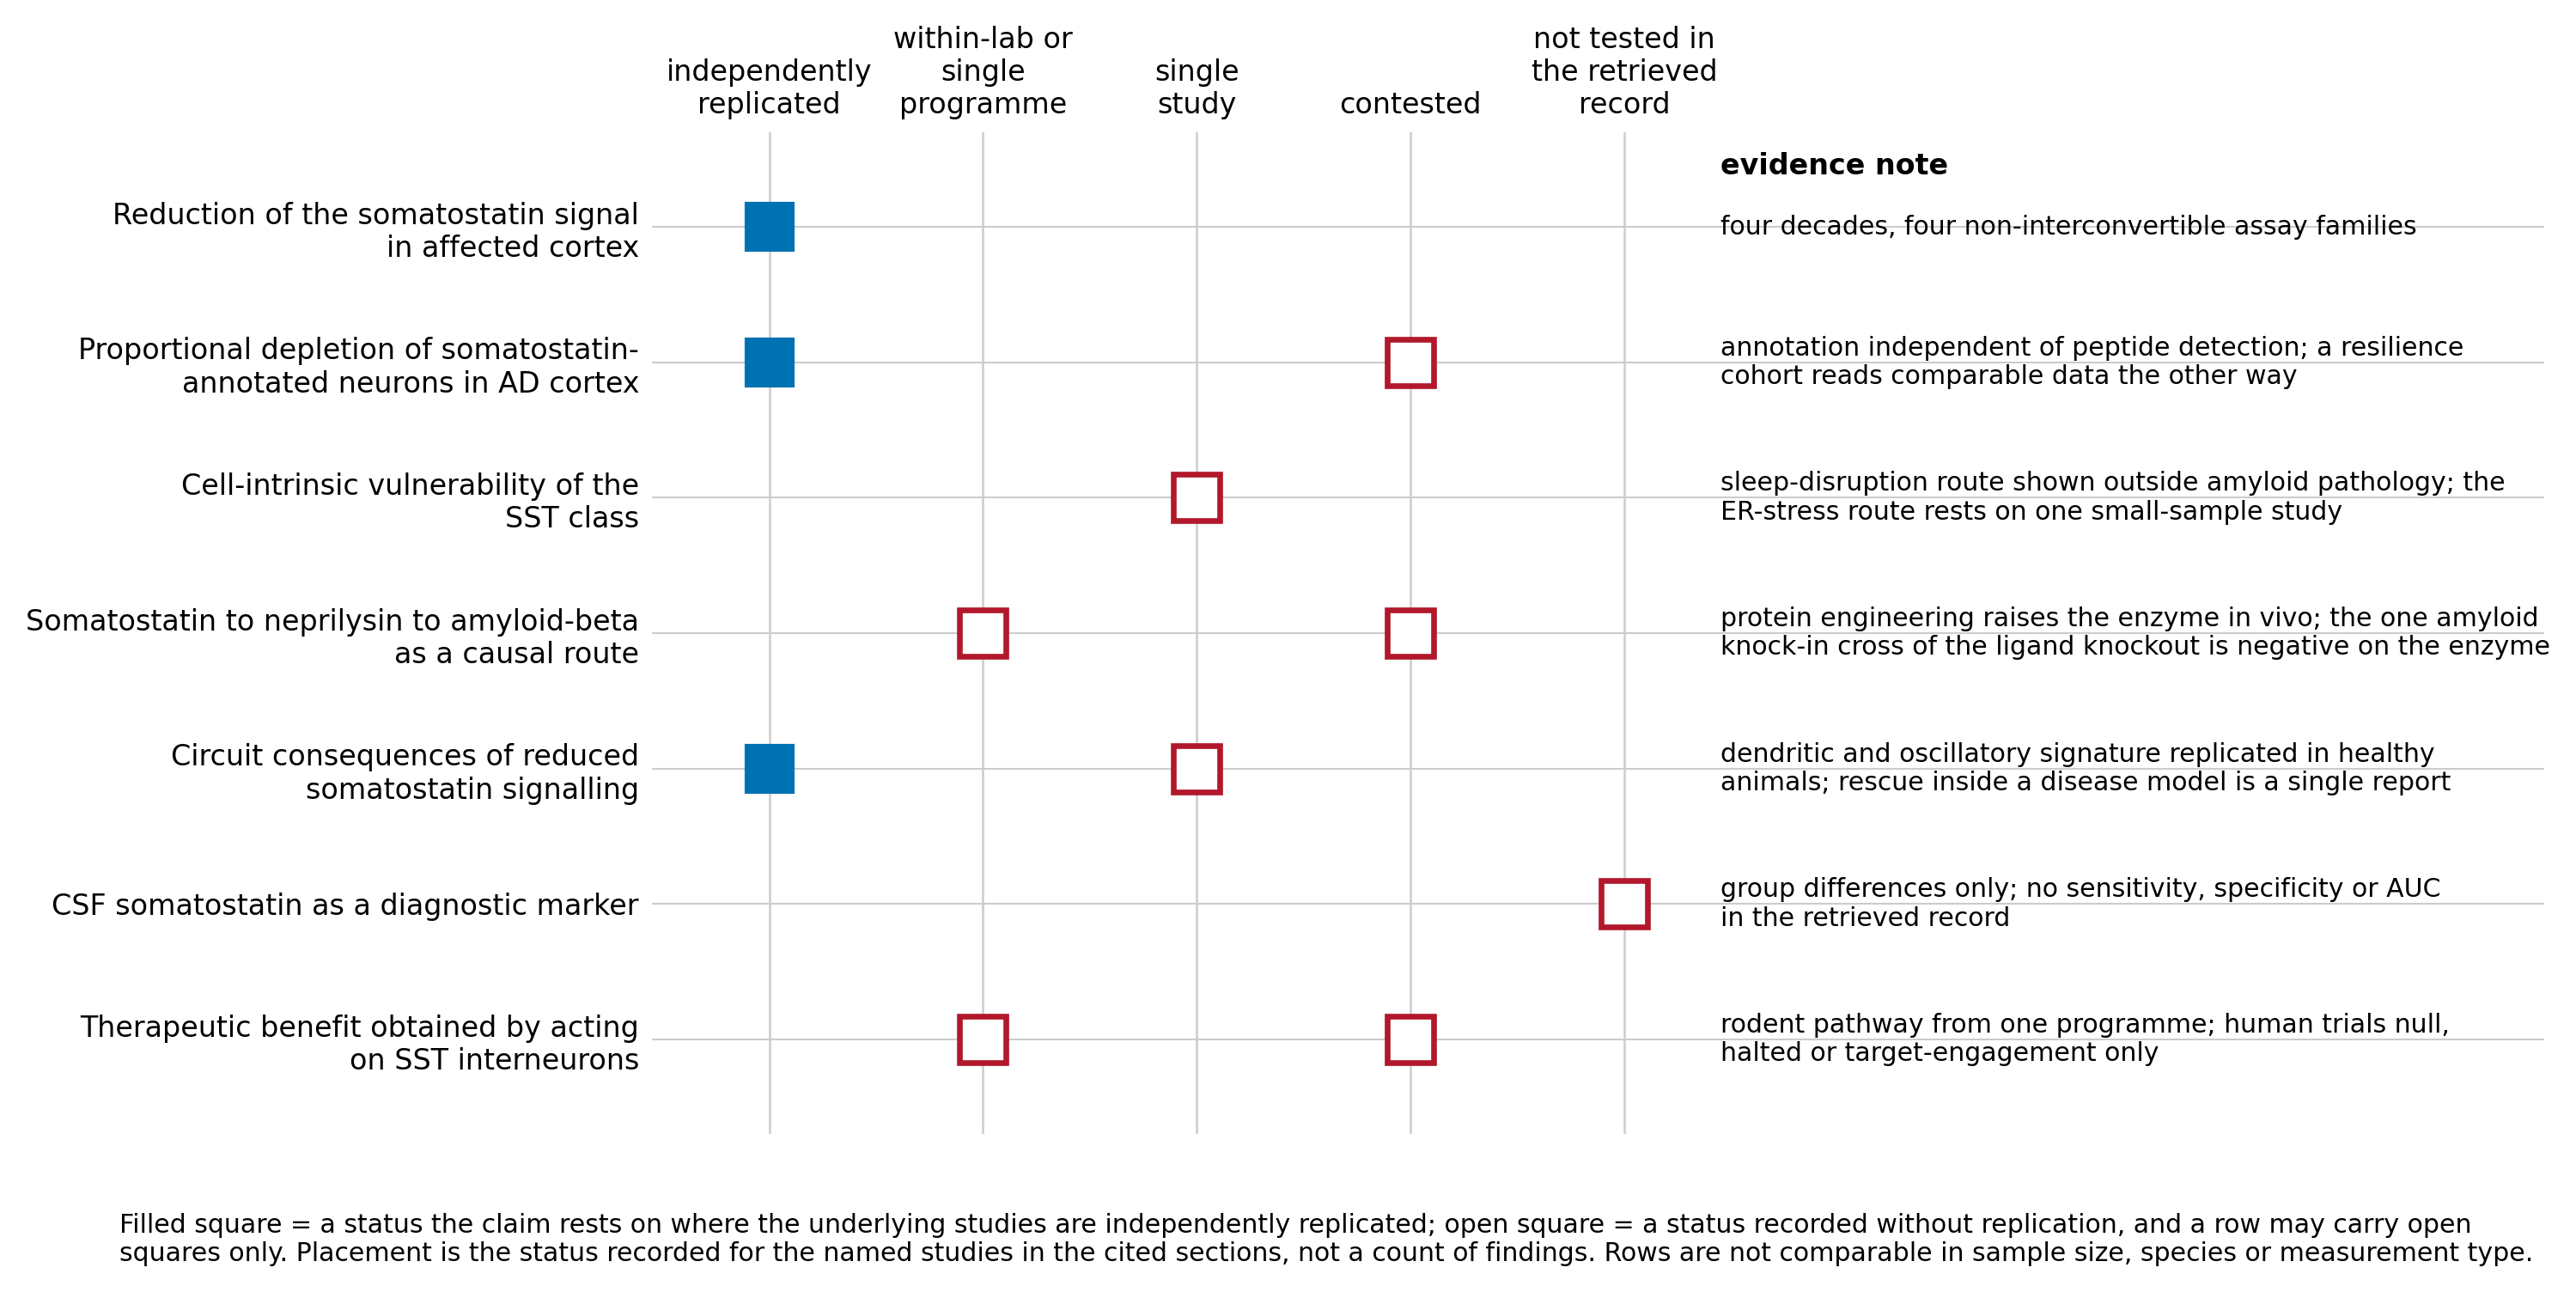
\includegraphics[width=\linewidth]{../figures/fig_sec12_evidence_confidence_by_claim.png}
\caption{\textbf{Confidence audit of the review's principal claims.} Seven rows, one per claim this review answers, against five status columns: independently replicated, within-lab or single programme, single study, contested, and not tested in the retrieved record. A filled square marks a status the claim rests on where the underlying studies are independently replicated; an open square marks a status recorded without replication, and a row may carry open squares only. Placements are the statuses recorded for the named studies in the cited sections, not counts over the literature. Row 1, reduction of the somatostatin signal in affected cortex, is the only row resting on replication alone. Row 2, proportional depletion of somatostatin-annotated neurons in AD cortex, carries a replicated marker resting on the single-nucleus cohorts set out in \ref{sec-human-evidence} rather than on the deconvolution mega-analysis \citep{Consens2022b}, and a contested one, because a resilience cohort reads comparable data the other way \citep{Castanho2025b}, because every test that separates a lost marker from a lost neuron is rodent \citep{Voelkl2022,Drake2024}, and because the human claim rests on immunoreactive counts in tension with pathology-matched peptidomics \citep{SaizSanchez2014,Morgan2024a}. Row 3, cell-intrinsic vulnerability of the SST class, sits at single study \citep{Raven2025}. Row 4, somatostatin to neprilysin to amyloid-beta as a causal route, sits at within-programme and contested \citep{Saito2005,Rofo2021}. Row 5, circuit consequences of reduced somatostatin signalling, carries a replicated marker for the dendritic and oscillatory signature in healthy animals and a single-study marker for rescue inside a disease model \citep{Chung2020}. Row 6, CSF somatostatin as a diagnostic marker, is the only row in the fifth column: no sensitivity, specificity or area under the curve exists in the retrieved record (\ref{sec-human-evidence}). Row 7, therapeutic benefit obtained by acting on SST interneurons, carries within-programme and contested status only \citep{Sandoval2019}, with the two human entries behind that row indirect rather than SST-directed: a synthesis of gamma stimulation, which acts on fast-spiking parvalbumin circuitry \citep{DePaolis2024}, and a non-cell-type-specific excitability-lowering trial \citep{Bakker2012}. Rows are not comparable in sample size, species or measurement type.}
\label{fig-sec12-evidence-confidence-by-claim}
\end{figure}

\begin{figure}[H]
\centering
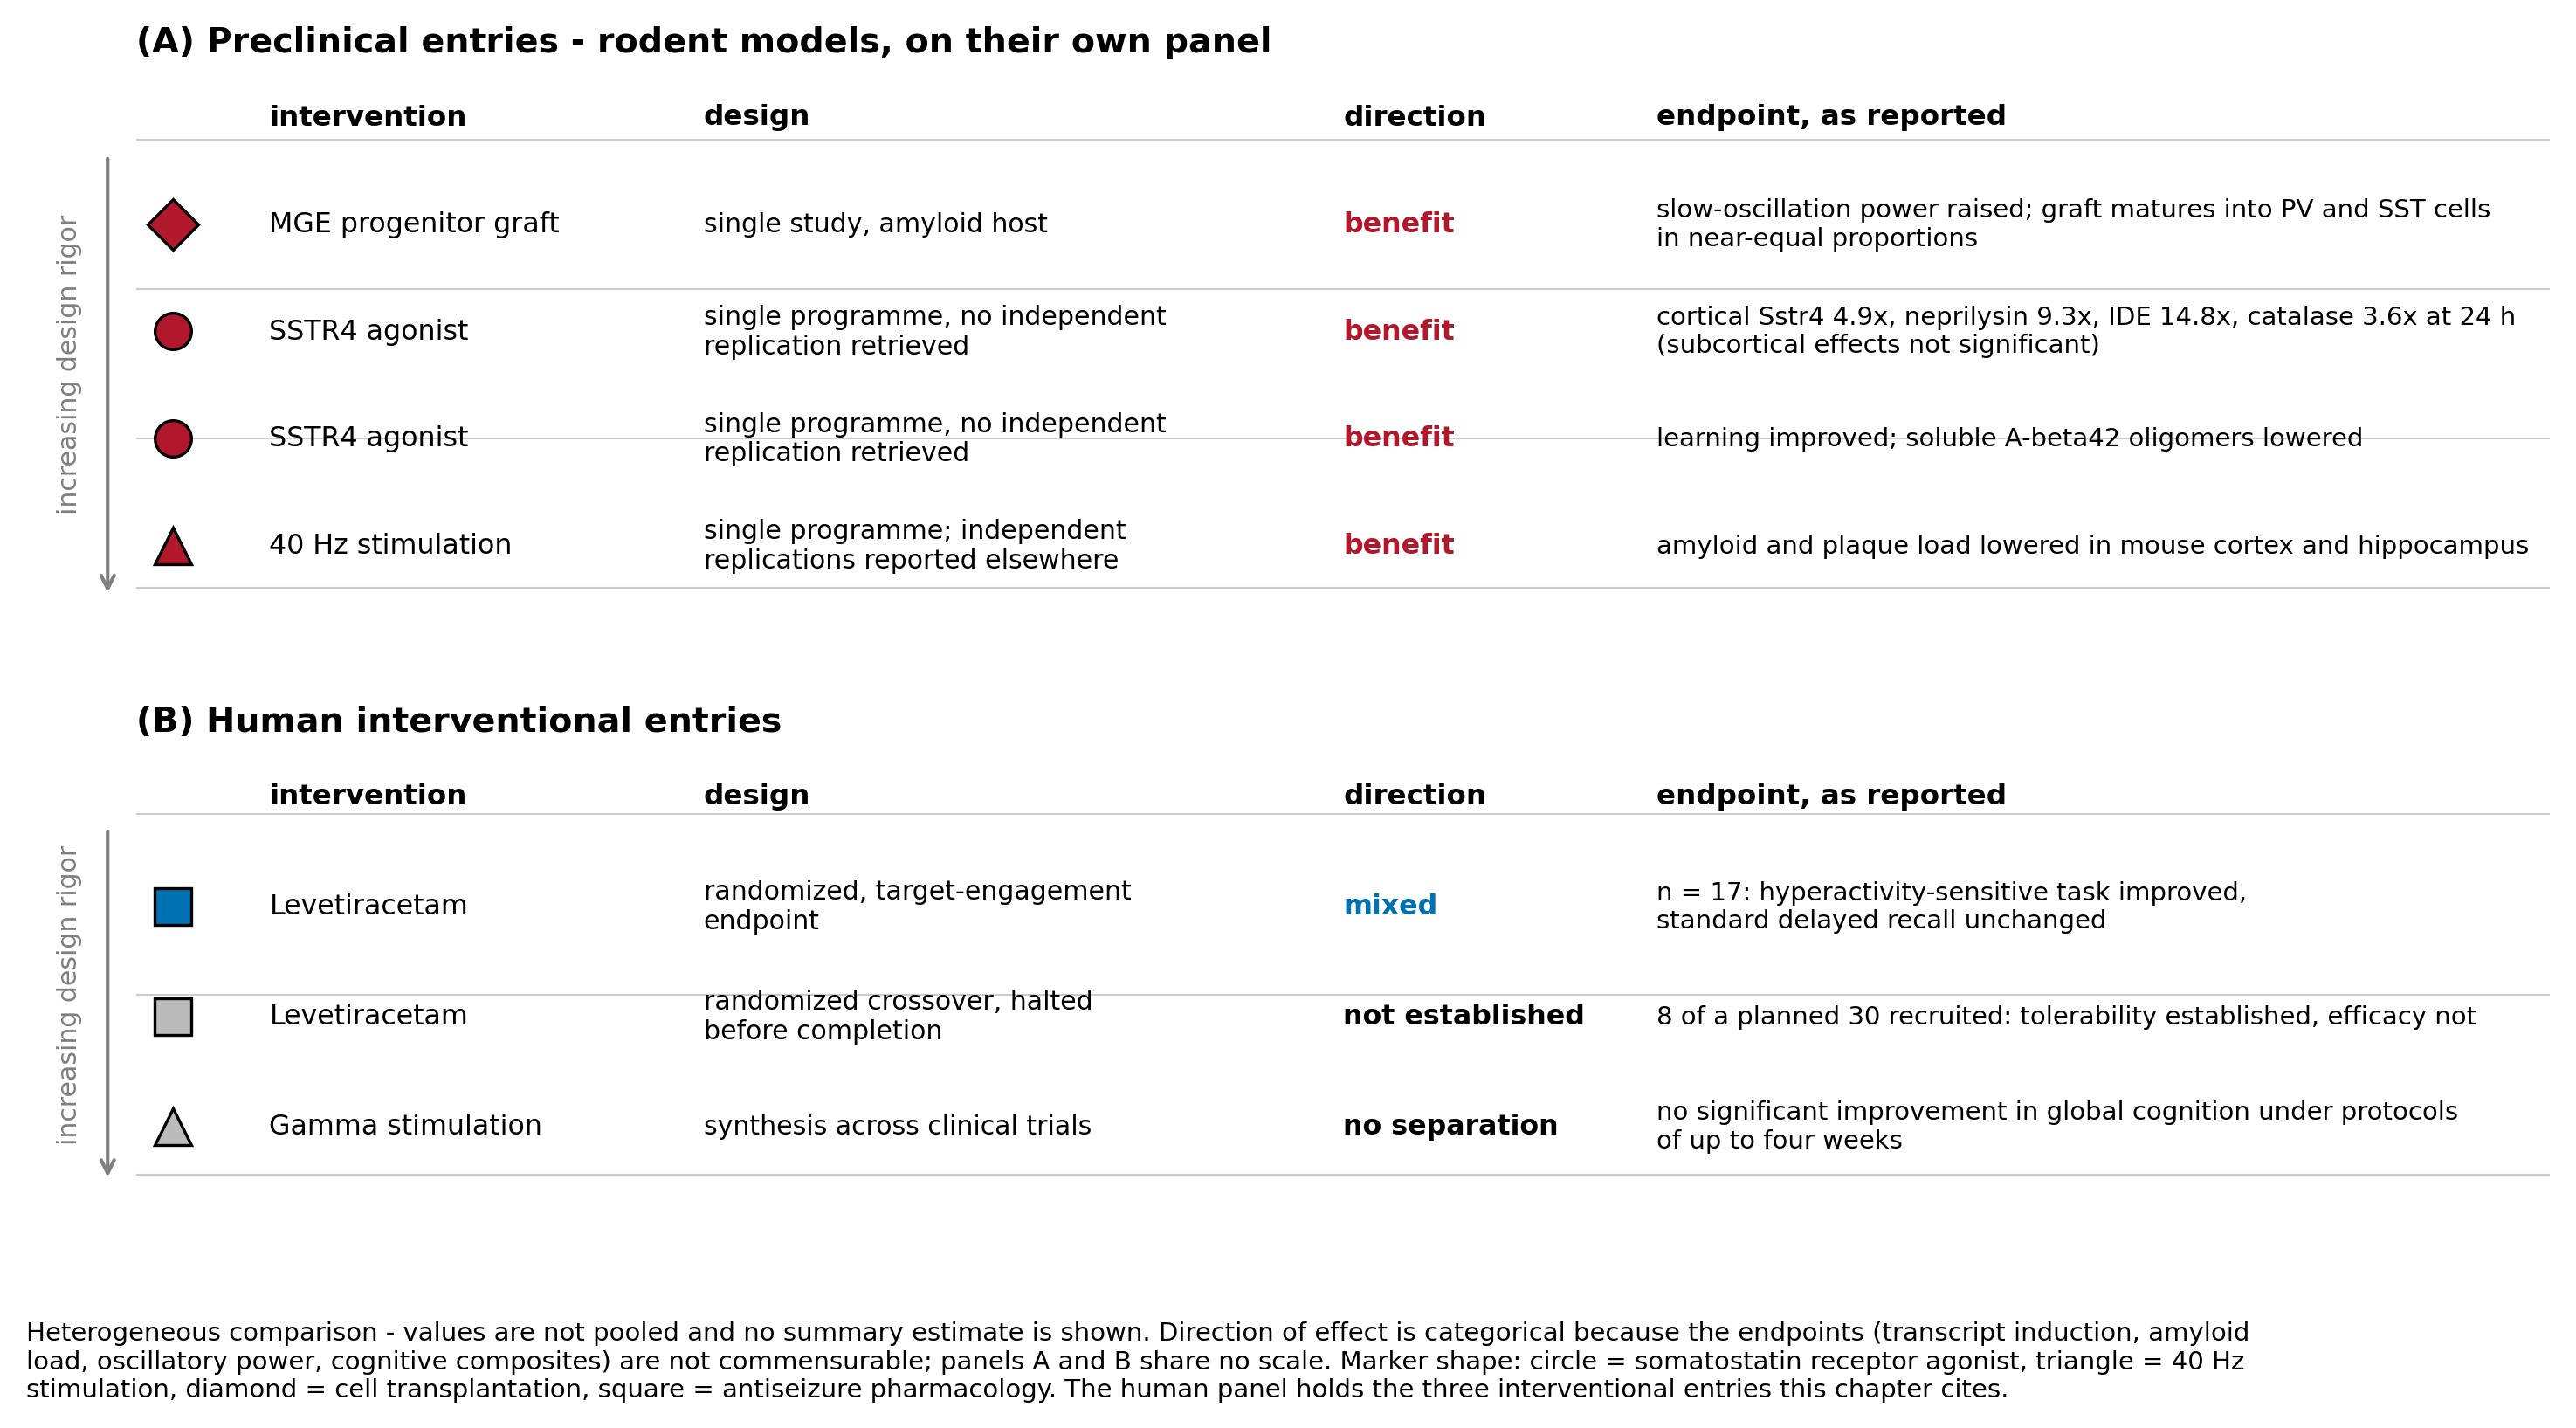
\includegraphics[width=\linewidth]{../figures/fig_sec12_intervention_effect_versus_design_rigor.png}
\caption{\textbf{Reported benefit against the design that produced it.} Direction of effect is categorical, not a magnitude, because the endpoints are not commensurable and are not pooled. Both panels are ordered by increasing design rigor, marked by the arrow at the left of each. (A) Preclinical entries, in the order drawn: grafted progenitors raising slow-oscillation power in an amyloid host while maturing into PV and SST cells in near-equal proportions, a single study \citep{Yokomizo2025a}; an SSTR4-selective agonist raising cortical \emph{Sstr4} 4.9-fold, neprilysin 9.3-fold, insulin-degrading enzyme 14.8-fold and catalase 3.6-fold at 24 h, with the corresponding subcortical effects not reaching significance \citep{Sandoval2019}; the same compound improving learning while lowering soluble A$\beta$42 oligomers \citep{Sandoval2013} --- both from one research programme, which is why those two rows are labelled single programme rather than replicated; and 40 Hz stimulation lowering amyloid and plaque load in mice \citep{Iaccarino2016}, extended to auditory and audiovisual delivery by the same programme \citep{Martorell2019}, with the independent replications of that amyloid endpoint given in \ref{sec-therapeutics}. (B) Human entries, ordered by increasing design rigor: a target-engagement trial in 17 patients in which the hyperactivity-sensitive task improved while standard delayed recall did not \citep{Bakker2012}; a randomized crossover trial halted after 8 of a planned 30 participants, establishing tolerability only \citep{Sen2024}; and a synthesis whose tabulated clinical gamma-stimulation trials report no significant change in overall cognition tests under protocols of up to four weeks, its authors' own conclusion being favourable to the technique \citep{DePaolis2024}. Heterogeneous comparison --- values are not pooled. Species, exposure duration, endpoint and control condition differ across every entry; panel A and panel B share no axis, and the human panel contains the three interventional entries this chapter cites, not the full inventory, which is given in \ref{sec-therapeutics}.}
\label{fig-sec12-intervention-effect-versus-design-rigor}
\end{figure}

The question this review opened with has a conditional answer. Somatostatin interneuron dysfunction is a shared feature of Alzheimer's disease whose causal contribution rests entirely on rodent knockout and agonist work, and it is a plausible contributor to circuit-level dysfunction in several other conditions; the shared selective death of the cell class is not established, and the experiments that would establish or refute it are specifiable, small in number, and have not been done. Until they are, the honest reading of the most reproducible neurochemical observation in this literature is that a signal has fallen --- and that the field has been reading a measurement as a cell.

\section{Methods}
\label{sec-methods}

This chapter documents how the review was produced. Every figure, rate and count below is read from a pipeline artifact --- the ten cluster evidence files, the twelve per-phase gate JSONs, the phase ledger, and the frame ledger for project \texttt{proj\_9238b857f2b8}. Values the pipeline did not record are marked as not recorded rather than estimated. The language model that executed every agent frame was \texttt{claude-opus-5}, run under the Expert Review Pipeline v29 protocol.

\begin{figure}[H]
\centering
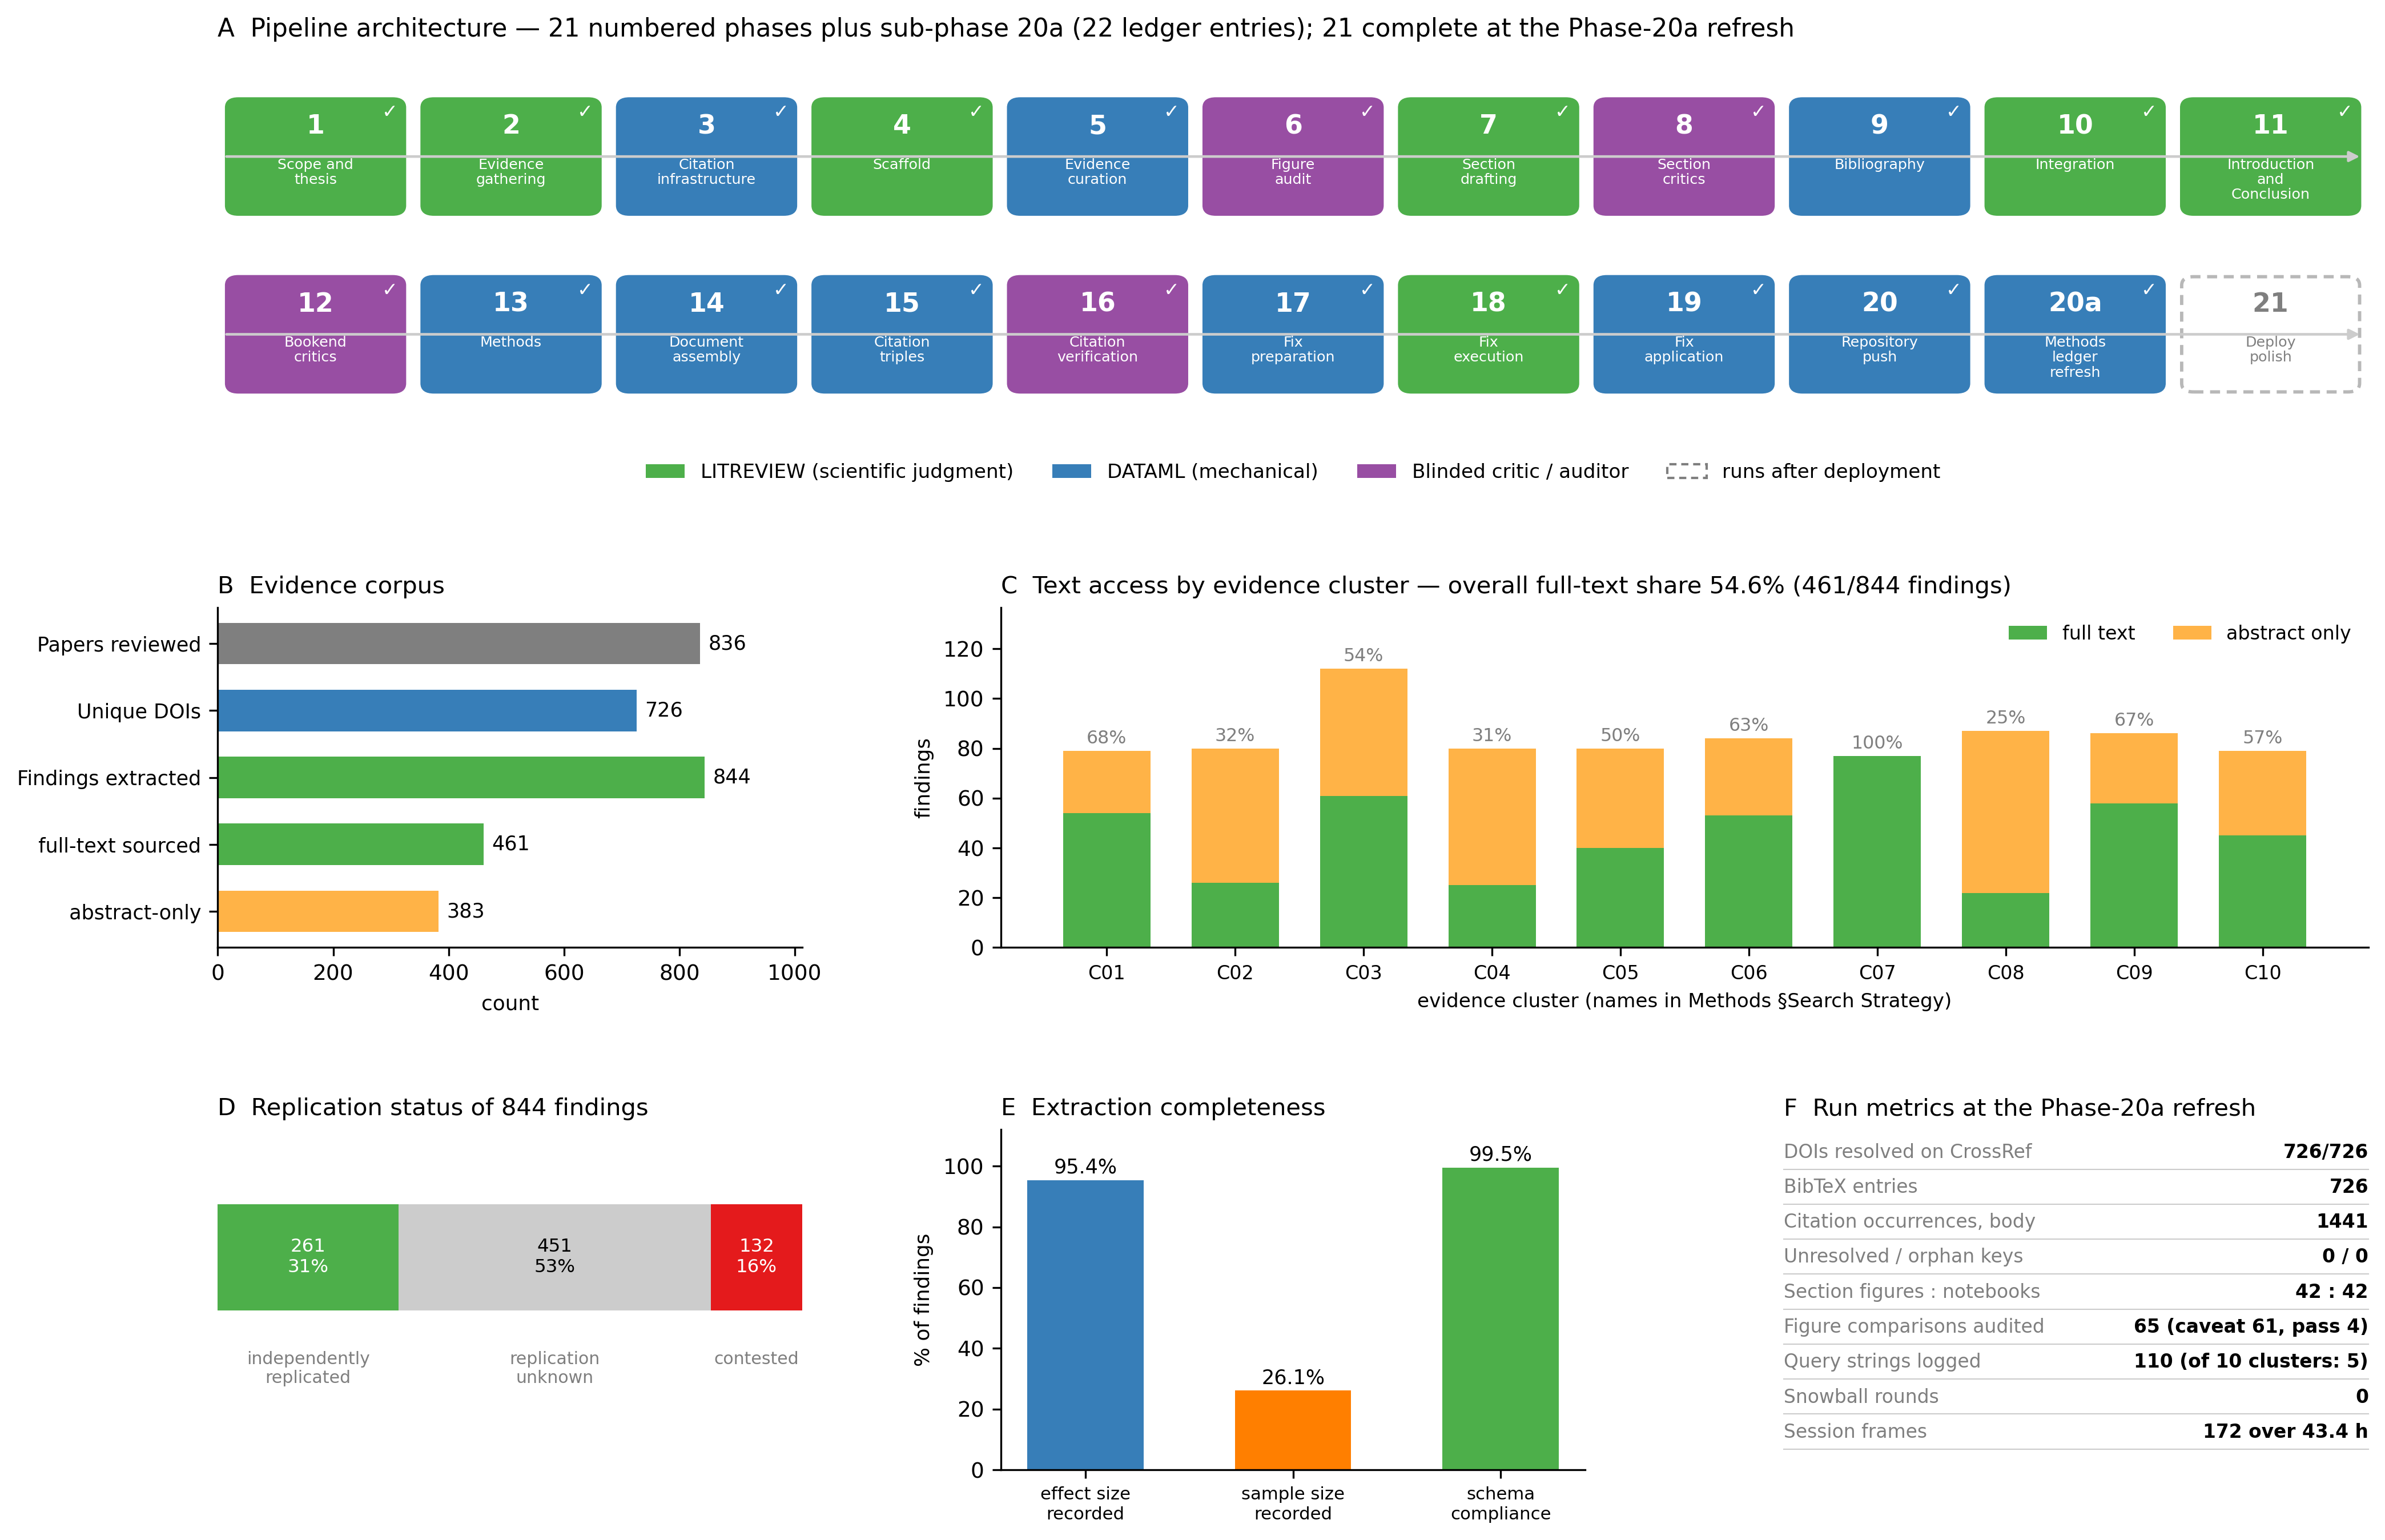
\includegraphics[width=\linewidth]{../figures/fig_methods_pipeline.png}
\caption{\textbf{Pipeline architecture and run metrics.} (A) The 21 numbered phases plus sub-phase 20a (22 ledger entries), coloured by the agent role that owns each phase; the single dashed entry, Phase 21, is the post-deployment polish gate, which runs against the served site after this commit. (B) Corpus sizes from the ten cluster evidence files. (C) Full-text versus abstract-only findings per cluster; the percentage above each bar is that cluster's full-text share. (D) Replication status assigned to the 844 findings. (E) Share of findings carrying an effect size, a sample size, and passing the strict Phase-2 schema check. (F) Headline run metrics at the Phase-20a refresh. All panels are generated by \texttt{figures/notebooks/fig\_methods\_pipeline.ipynb} from \texttt{provenance/pipeline\_metrics.json}.}
\label{fig-methods-pipeline}
\end{figure}

\subsection{Review Request}
\label{sec-methods-review-request}

The review was initiated by a single user request that fixed the topic, the audience and the high-level argument arc. That request is preserved byte-for-byte in \texttt{provenance/review\_request.md}, alongside a SHA256 of the raw bytes and an editorial note listing any mechanical reflow applied. Phase 1 translated it into the structured scope record (\texttt{gate\_scope.json}): the title \emph{Somatostatin Interneurons in Neurodegenerative Disease}, ten evidence clusters, twelve body sections, and the evidence parameters reproduced in [Inclusion and Exclusion Criteria](\#sec-methods-inclusion).

The captured request, reproduced verbatim from \texttt{provenance/review\_request.txt}

(1755 bytes, SHA256 \texttt{3bf90056d1521298f01529391c468e9113baa7b2f49e04149d8bbdafd6b6c738}):

\begin{Verbatim}[breaklines,breakanywhere]
Start a comprehensive critical literature review titled: "Somatostatin Interneurons in Neurodegenerative Disease"

GitHub Repository: https://github.com/AllenNeuralDynamics/ComputationalReviewSSTdisease
Clone it into the workspace. The files in its skills/ folder define the complete pipeline;
nothing needs to be installed — follow the "Runtime: Claude Science" section of the orchestrator.

skills/comprev-orchestrator-v29.md — The coordinator protocol. Read this FIRST.
It defines the routing across 21 phases, gate artifacts, and the session protocol.
Per-phase rules live in the agent skills, which the coordinator passes to sub-agents.

skills/comprev-reviewer-agent.md — The worker skill for LITREVIEW roles.
Pass it to every LITREVIEW delegation.

skills/comprev-figure-construction.md — Section writers use it for figure production.

Push all outputs to this repo in Phase 20.

Table of Contents:
1. Introduction
2. SST Interneuron Identity: Transcriptomic Subtypes, Connectivity, and Somatostatin Receptor Signaling
3. Selective Vulnerability of SST Interneurons in Aging and Neurodegeneration
4. Alzheimer's Disease: SST Loss, Amyloid-β and Neprilysin, Tau, and Network Hyperexcitability
5. Parkinson's Disease and Lewy Body Dementias
6. Huntington's Disease and Striatal SST Interneurons
7. ALS, Frontotemporal Dementia, and Other Neurodegenerative Conditions
8. Circuit Consequences: Dendritic Inhibition, Oscillations, Sleep, and Memory
9. Human Evidence: Postmortem Pathology, Single-Nucleus Atlases, and CSF Somatostatin as a Biomarker
10. Therapeutic Strategies: Somatostatin Receptor Agonists, Interneuron-Targeted Interventions, and Neuromodulation
11. Conflicting Evidence, Model Limitations, and Open Questions
12. Conclusion
\end{Verbatim}

\subsection{Search Strategy}
\label{sec-methods-search}

Searches were organised around the ten evidence clusters defined in \texttt{gate\_scope.json}, each feeding one or more body sections. Retrieval ran entirely against public REST endpoints called from Python's standard library, because the \texttt{requests} and \texttt{certifi} packages were absent from the execution environment and package installation was unavailable; HTTPS therefore used an unverified SSL context. The endpoints recorded in \texttt{gate\_evidence\_compliance.json} are:

\begin{itemize}
\item Europe PMC REST search, \texttt{https://www.ebi.ac.uk/europepmc/webservices/rest/search} with \texttt{resultType=core} --- the primary discovery endpoint for every cluster
\item Europe PMC full-text XML, \texttt{https://www.ebi.ac.uk/europepmc/webservices/rest/\{PMCID\}/fullTextXML}
\item NCBI E-utilities, \texttt{https://eutils.ncbi.nlm.nih.gov/entrez/eutils/efetch.fcgi?db=pmc}
\item CrossRef, \texttt{https://api.crossref.org/works/\{doi\}}, for bibliographic metadata
\item an open-access full-text fetch helper backed by Unpaywall and PMC
\end{itemize}

Coverage was therefore Europe PMC-dominant. No contact email was available to the pipeline, so CrossRef and NCBI were called without a \texttt{mailto} parameter.

\begin{table}[H]
\centering
\small
\begin{tabular}{llrrrr}
\toprule
\textbf{Cluster} & \textbf{Topic} & \textbf{Papers reviewed} & \textbf{Findings} & \textbf{Full text} & \textbf{Query strings logged} \\
\midrule
C01 & SST identity \& SSTR signaling & 79 & 79 & 54 (68\%) & 6 \\
C02 & Selective vulnerability \& aging & 80 & 80 & 26 (32\%) & not recorded \\
C03 & Alzheimer's disease & 108 & 112 & 61 (54\%) & not recorded \\
C04 & Parkinson's / Lewy body & 79 & 80 & 25 (31\%) & not recorded \\
C05 & Huntington's disease & 80 & 80 & 40 (50\%) & not recorded \\
C06 & ALS / FTD / other & 84 & 84 & 53 (63\%) & 7 \\
C07 & Circuit consequences & 77 & 77 & 77 (100\%) & 49 \\
C08 & Human postmortem, snRNA, CSF & 85 & 87 & 22 (25\%) & 21 \\
C09 & Therapeutic strategies & 85 & 86 & 58 (67\%) & 27 \\
C10 & Conflicts \& methodological caveats & 79 & 79 & 45 (57\%) & not recorded \\
\textbf{Total} &  & \textbf{836} & \textbf{844} & \textbf{461} & \textbf{110} \\
\bottomrule
\end{tabular}
\end{table}

Deduplication across clusters reduced 836 reviewed papers to \textbf{726 unique DOIs}, the figure certified by the Phase-3 citation infrastructure gate and carried unchanged into the bibliography.

\textbf{Search logging is partial, and this limits what can be reported here.} Five of the ten clusters recorded query strings in their evidence file; five

(C02, C03, C04, C05, C10) recorded none. Across the five that did,

110 query strings are on record. Of those, 41 come from cluster C07's original keyword sweep; the remaining 69 were logged during the Phase 2V disconfirming-search remediation, not during the original Phase 2 sweep. Per-query result counts exist for 60 of the 110 logged queries --- C07's 41 original-sweep strings carry no hit counts. For the six clusters with no original-sweep query log, \textbf{per-query result counts are not available for the original searches, and the query strings themselves were not recorded.} They are not reconstructed here.

Candidate screening volume was recorded for two clusters only: 2,218 candidates screened in C01 and 624 candidates examined in C02. For the other eight clusters the pre-screening candidate count is not recorded.

The disconfirming sweeps were capped per query rather than run to exhaustion. Where the cap is recorded it was 50 records examined per query in C01, 13--50 in C06, and 8--25 in C09; C08 recorded records retrieved per query, ranging 1--198. C07's eight contradiction queries yielded 217 new unique candidates, of which four were screened in. Database-reported hit counts for these queries run into the thousands (for example 10,235 and 19,798 for two C01 queries), so the examined fraction is a small and deliberately bounded sample of each query's result set.

\texttt{evidence\_parameters.snowball\_rounds} was \textbf{0}: no forward or backward citation chasing was performed in either direction. Cluster C07's evidence file records \texttt{snowball\_rounds\_run: 0} independently.

\subsection{Inclusion and Exclusion Criteria}
\label{sec-methods-inclusion}

The scope record fixed these evidence parameters:

\begin{itemize}
\item \texttt{min\_papers\_per\_cluster}: \textbf{70} (a floor, not a target)
\item \texttt{snowball\_rounds}: \textbf{0}
\item \texttt{saturation\_criterion}: not set
\item \texttt{total\_bibliography\_target}: not set; \texttt{bibliography\_target\_is\_hard\_floor}: true
\end{itemize}

Every cluster cleared the floor, with per-cluster paper counts from 77 to

\begin{enumerate}
\item Inclusion required that a record be
\end{enumerate}

primary research within the cluster's declared scope and that the sentence supporting each extracted claim be present verbatim in the retrieved text. Peripheral endocrine and oncology records were excluded at screening in the clusters whose screening rule is recorded. Preprint--journal duplicate pairs were resolved in favour of the published version.

Nineteen search-failure records are logged across the ten cluster packages. Their dispositions, counted from the \texttt{search\_failures} arrays, are:

\begin{table}[H]
\centering
\small
\begin{tabular}{lr}
\toprule
\textbf{Disposition} & \textbf{Records} \\
\midrule
Paper retained with \texttt{text\_access = abstract\_only} after full text could not be obtained & 6 \\
Paper excluded and the shortfall logged as an evidence gap & 7 \\
Evidence gap logged with no paper added & 4 \\
Preprint excluded in favour of its published version & 1 \\
Previously extracted finding removed rather than re-worded & 1 \\
\textbf{Total} & \textbf{19} \\
\bottomrule
\end{tabular}
\end{table}

No paper was excluded solely because its full text was unavailable: where an abstract carried the claim verbatim, the paper was retained and marked abstract-only. Papers for which neither full text nor a usable abstract could be retrieved appear in the eleven evidence-gap records above rather than in the findings.

\subsection{Full-Text Retrieval}
\label{sec-methods-retrieval}

Full-text retrieval was attempted for every candidate through Europe PMC \texttt{fullTextXML}, NCBI E-utilities \texttt{efetch} against PMC, and an Unpaywall/PMC-backed fetch helper. \textbf{The publisher and aggregator APIs named in the pipeline template were not all used: no Elsevier, Springer Nature, OpenAlex or NCBI API key was available in this environment, so those sources were not queried.} Retrieval rates per source were not recorded separately; only the resulting per-finding \texttt{text\_access} label is.

Of 844 findings, \textbf{461 are sourced from a retrieved article body and 383 from an abstract}, an overall full-text share of \textbf{54.6\%}. The share varies sharply by cluster, from \textbf{100\% in C07} (circuit consequences) to \textbf{25\% in C08} (human postmortem, single-nucleus and CSF evidence); C02 (32\%) and C04 (31\%) are similarly constrained. The shortfall is concentrated in pre-2000 closed-access postmortem and CSF literature, which PMC holds only as scanned records: the recorded failure modes are PMC returning a sub-15 KB record with no \texttt{<body>} element, HTTP 500 from \texttt{fullTextXML}, and DOIs with no PMCID at all.

A 15 KB size-validation threshold is recorded in the evidence files for five clusters

(C01, C02, C04, C07, C10): a retrieval below that size, or lacking a \texttt{<body>} element, was

treated as a failed full-text fetch and the paper was marked abstract-only. The remaining five clusters do not record whether the threshold was applied. Where a PDF was the only available form, text was recovered by inflating the PDF content streams with \texttt{zlib} and extracting literal strings, because no PDF library could be installed.

Source-sentence validation was run per cluster: each claim sentence was asserted to be a verbatim substring of the Europe PMC abstract (for abstract-only findings) or of the retrieved article body (for full-text findings), with full-text sentences additionally asserted absent from the abstract.

\subsection{Evidence Extraction}
\label{sec-methods-extraction}

Each cluster produced an evidence file in a fixed schema. Every finding carries \texttt{doi}, \texttt{cite\_key}, \texttt{claim}, \texttt{claim\_source\_sentence}, \texttt{evidence}, \texttt{effect\_size}, \texttt{effect\_size\_source\_sentence}, \texttt{n}, \texttt{study\_system}, \texttt{replication\_status}, \texttt{replication\_evidence\_dois} and \texttt{text\_access}. Packages additionally carry \texttt{conflicts}, \texttt{unreplicated\_claims}, \texttt{evidence\_gaps}, \texttt{figure\_data}, \texttt{search\_failures} and \texttt{source\_sentence\_validation}.

\begin{table}[H]
\centering
\small
\begin{tabular}{lr}
\toprule
\textbf{Metric} & \textbf{Value} \\
\midrule
Findings extracted & 844 \\
Unique DOIs & 726 \\
Conflicts recorded & 90 \\
Figure-data comparisons & 52 (spanning 190 papers) \\
Findings with an effect size & 805 (95.4\%) \\
Findings with a sample size & 220 (26.1\%) \\
Strict schema compliance & 99.526\% (840/844) \\
\bottomrule
\end{tabular}
\end{table}

The gap between the effect-size rate (95.4\%) and the sample-size rate (26.1\%) reflects the source literature: abstracts frequently state a magnitude without a cohort size, and the pipeline recorded \texttt{n} only where it was stated in the retrieved text.

Replication status across the 844 findings:

\begin{table}[H]
\centering
\small
\begin{tabular}{lrr}
\toprule
\textbf{Status} & \textbf{Findings} & \textbf{Share} \\
\midrule
Independently replicated & 261 & 30.9\% \\
Replication unknown & 451 & 53.4\% \\
Contested & 132 & 15.6\% \\
\bottomrule
\end{tabular}
\end{table}

Phase 5 reorganised the cluster packages into twelve per-section packages organised by argument, carrying 809 distinct DOI--sentence records; 64 DOIs appear in more than one section, and in no case does the same DOI contribute the same source sentence to two sections.

Four field-level corrections were applied to evidence files after their gates had passed. Each is logged in the affected package's own \texttt{corrections} array rather than applied silently:

\begin{itemize}
\item \textbf{Davies1990} (\texttt{evidence\_section\_09.json}) --- the \texttt{claim} field had extended a fibre-length null result to perikaryal counts; corrected in the section package, with the certified cluster file left unmodified because the defect was introduced downstream.
\item \textbf{Ouellet2014} (\texttt{evidence\_section\_01.json}) --- \texttt{study\_system} and \texttt{claim} corrected against the CrossRef title for \texttt{10.3389/fnana.2014.00040}; the study is rat primary auditory cortex, not mouse cortex. The correction aligns this package with the section 08 package for the same DOI.
\item \textbf{Frankowski2022} (\texttt{evidence\_section\_01.json}) --- supplementary source sentences added, traced to the section 07 package for the same DOI.
\item \textbf{Hofling2019} (\texttt{evidence\_section\_12.json}) --- a reported range traced to the section 04 package's source sentence for the same DOI.
\end{itemize}

\subsection{Citation Verification}
\label{sec-methods-citation-verification}

Four mechanical verification passes ran, all against live databases and none of them sampled.

\textbf{Phase 3 --- citation infrastructure.} All 726 unique DOIs were re-queried against \texttt{api.crossref.org/works/\{doi\}}; 726 resolved. Cite keys were derived mechanically from the CrossRef first-author surname and publication year, giving zero orphan DOIs and zero unused keys.

\textbf{Phase 9 --- bibliography.} The 726-entry \texttt{references.bib} was checked against a fresh CrossRef fetch of all 726 DOIs on fourteen named checks, all of which passed: DOI resolution, first-author surname match, title similarity

(threshold 0.85, minimum observed 0.875), exact year match, journal match for the 700 journal

articles, volume/issue/pages match, pure-ASCII encoding, key uniqueness, key derivation, and contamination screening. Across the ten body sections, \textbf{1441 citation occurrences resolve to 726 distinct keys}, with 0 unresolved keys and 0 uncited bibliography entries.

\textbf{Phase 15 --- citation triples.} Extraction was exhaustive rather than sampled: one triple per individual cite key, \textbf{1,534 in total}, each pairing a key with the sentence that carries it and with the bibliography record behind it. The count was checked against the document two independent ways --- by counting cite keys across all \texttt{\{cite:p\}} and \texttt{\{cite:t\}} directives and by counting the extracted triples --- and the two agree.

\textbf{Phase 16 --- claim-level verification.} Every triple was adjudicated against the cited paper's own text. The adjudication returned \textbf{1,351 VERIFIED, 122 MINOR, 25 MISATTRIBUTED, 0 CHIMERIC and 0 HALLUCINATED}, with a further \textbf{36 records unverifiable because the source text could not be retrieved}. No citation in this review resolves to a non-existent paper, and none resolves to a different paper than the one named.

\textbf{Phases 17 and 18 --- fix preparation and execution.} The 147 defect records were consolidated into \textbf{118 fix requests}, of which \textbf{113 were applied, 5 were not applied and 0 failed}. Four of the five unapplied requests were conditional deletions: each proposed removing a value as unsourceable, and in each case the value turned out to be carried by a source sentence in the section's evidence file, so the value was kept rather than deleted. The fifth proposed deleting a duplicate bibliography entry; it was declined because the entry is still cited three times in the Alzheimer's disease section, and removing it would have left those citations unresolved.

\textbf{Final state.} The bibliography holds \textbf{726 entries against 726 distinct cite keys, with zero unresolved keys and zero uncited entries in both the MyST content and the LaTeX manuscript}, and the file is pure ASCII.

\textbf{What this does not establish.} The 36 unverifiable records are a limit of coverage, not a clean result. They are claims whose source text could not be retrieved --- concentrated in the closed-access literature that this review reads at abstract level --- and they remain unchecked rather than checked and passed. The verified share above is a share of the 1,498 triples that could be checked, and the honest reading of the remainder is that nobody looked.

\subsection{Pipeline Execution}
\label{sec-methods-pipeline}

This subsection is rendered at sub-phase 20a, immediately before the repository push, from the project frame ledger and the gate artifacts in \texttt{provenance/}. It supersedes the draft snapshot written at Phase 13, which covered Phases 1 to 12 only.

\begin{itemize}
\item \texttt{snapshot\_phase}: \textbf{20a}
\item \texttt{model\_version}: \textbf{\texttt{claude-opus-5}}
\item Pipeline: \textbf{Expert Review Pipeline v29}
\end{itemize}

\textbf{Frame ledger.} The project frame ledger for \texttt{proj\_9238b857f2b8} holds \textbf{172 frames}: 155 completed, 8 cancelled, 7 failed and 2 still processing when this chapter was refreshed. The ledger records a single \texttt{agent\_name} value for every frame, so a per-agent frame breakdown cannot be derived from it; the per-phase ownership shown in panel A of \ref{fig-methods-pipeline} comes from the pipeline specification, not from the frame records.

\textbf{Wall clock.} First frame created \textbf{2026-10-16T04:19:11.625Z}; most recent frame \textbf{2026-10-17T23:45:45.218Z}; elapsed \textbf{43.44 h}.

\textbf{Phase ledger.} 21 of 22 entries complete.

\begin{table}[H]
\centering
\small
\begin{tabular}{llll}
\toprule
\textbf{Phase} & \textbf{Description} & \textbf{Status} & \textbf{Key output} \\
\midrule
1 & Scope and thesis & Complete & \texttt{gate\_scope.json} --- twelve sections, ten evidence clusters \\
2 & Evidence gathering & Complete & \texttt{gate\_evidence\_compliance.json} --- 844 findings over 726 unique DOIs \\
3 & Citation infrastructure & Complete & \texttt{gate\_citation\_infrastructure.json} --- 726 DOIs mapped to cite keys \\
4 & Section planning & Complete & \texttt{gate\_scaffold\_approved.json} --- section plans and figure registry \\
5 & Evidence curation & Complete & \texttt{gate\_evidence\_curated.json} --- twelve per-section evidence files \\
6 & Figure audit & Complete & \texttt{gate\_figure\_audit.json} --- 65 cross-study comparisons audited \\
7 & Section drafting & Complete & \texttt{gate\_sections\_drafted.json} --- twelve sections drafted \\
8 & Section critics & Complete & \texttt{gate\_critic\_complete.json} --- 87 must-fix items, then 14, then 0 \\
9 & Bibliography & Complete & \texttt{gate\_bibliography.json} --- 726 entries, pure ASCII \\
10 & Integration & Complete & \texttt{gate\_integration.json} --- cross-section reconciliation \\
11 & Introduction and Conclusion & Complete & \texttt{gate\_intro\_conclusion.json} --- both bookends written \\
12 & Bookend critics & Complete & \texttt{gate\_bookend\_critic.json} --- 0 must-fix after three blinded rounds \\
13 & Methods & Complete & this chapter \\
14 & Document assembly & Complete & \texttt{gate\_assembly.json} --- 16 content files, 43 figures, 43 notebooks \\
15 & Citation triples & Complete & 1,534 triples, one per cite key \\
16 & Citation verification & Complete & 1,351 verified, 122 minor, 25 misattributed, 0 chimeric, 0 hallucinated, 36 unverifiable \\
17 & Fix preparation & Complete & \texttt{fix\_requests.json} --- 118 requests from 147 defect records \\
18 & Fix execution & Complete & \texttt{provenance/fix\_execution\_log.json} --- 113 applied, 5 not applied, 0 failed \\
19 & Fix application & Complete & site build run: 16 of 16 pages, zero citation-link errors \\
20 & Repository push & Complete & this commit \\
20a & Methods ledger refresh & Complete & this subsection and the architecture figure above \\
21 & Deploy polish & Runs after deployment & post-deployment gate against the served site \\
\bottomrule
\end{tabular}
\end{table}

\textbf{Phases completed.} Twenty-one of the twenty-two ledger entries are complete --- Phases 1 through 20 and sub-phase 20a --- each with its gate artifact preserved in \texttt{provenance/} as \texttt{gate\_*.json}. The twenty-second entry, Phase 21, is the post-deployment polish gate: it runs against the served site after this commit is deployed, and its gate artifact is written then.

\textbf{Site build.} The MyST site build was executed against this content with \texttt{mystmd} 1.11.0: \textbf{16 of 16 pages built, zero citation-link errors, zero missing images and zero unknown directives}. An earlier assembly record stated that the build had been deferred because no JavaScript runtime was available; that record was wrong, the runtime was present, and the build result above replaces it.

Two gates record that an earlier iteration failed and was remediated: the Phase-2 evidence compliance gate passed on its third iteration after a source-provenance remediation, and the Phase-7 MyST gate passed on its third iteration. The Phase-8 section critics opened 87 must-fix items in the first round, 14 after the re-check and 0 at the final remediation; the Phase-12 bookend critics closed at 0 must-fix after three blinded rounds.

\subsection{Figure Reproducibility}
\label{sec-methods-figures}

Every figure in the body of this review is generated from the archived evidence files by a notebook committed alongside it. The repository holds \textbf{42 section figures and 42 notebooks} --- a one-to-one correspondence, with no figure lacking a notebook and no notebook lacking a figure --- plus \ref{fig-methods-pipeline} and its notebook, which reads \texttt{provenance/pipeline\_metrics.json}.

All notebooks import the shared style module \texttt{figures/notebooks/shared\_style.py}, which fixes the palette, font, line weights and 300 dpi output. The palette is colourblind-accessible: a reduced ColorBrewer Set1 for categorical primaries and an Okabe--Ito set for the document-wide cell-type colours (SST \texttt{\#0072B2}, PV \texttt{\#D55E00}, VIP \texttt{\#CC79A7}, NPY/NOS \texttt{\#009E73}, pyramidal \texttt{\#666666}, mixed GABAergic \texttt{\#56B4E9}), with a fixed three-colour encoding for the direction of a reported change.

Cross-study comparison figures were audited blind before drafting. Of 65 proposed comparisons, 4 passed unconditionally, 61 were admitted with a mandatory caveat carried into the caption, and 0 were returned for redesign.

\subsection{Pipeline Skills}
\label{sec-methods-skills}

The pipeline is encoded as 20 version-controlled skill files committed to this repository under \texttt{skills/}. Each is a markdown specification loaded by the relevant agent at the relevant phase, so re-running a phase requires only the skill plus the upstream artifacts. Information barriers are enforced by omission: section writers never load the critic rubric, figure auditors never load the argument arc, and validator skills are loaded only by the gate frames that evaluate an actor's output. The table below is generated by scanning the live \texttt{skills/} directory and reading each file's leading description.

\begin{table}[H]
\centering
\small
\begin{tabular}{ll}
\toprule
\textbf{Skill} & \textbf{Role} \\
\midrule
\texttt{comprev-citation-validator.md} & Citation Validator --- Binary Gate for Phases 3 and 9. \\
\texttt{comprev-critic.md} & Section Critic Protocol. \\
\texttt{comprev-curation-validator.md} & Curation Validator --- Binary Gate for Phase 5. \\
\texttt{comprev-dataml-phases.md} & DATAML Phase Protocols. \\
\texttt{comprev-deploy-polish.md} & Phase 21 (post-deployment) UX validation skill. Runs after Phase 20 push to main confirms green build. Catches deployment-class defects (per-page rendering, plugin data-binding, figure dropdown completeness, link health, asset paths, frontmatter visibility) that compile-time checks miss. \\
\texttt{comprev-evidence-gathering.md} & Evidence Gathering Protocol. \\
\texttt{comprev-evidence-validator.md} & Evidence Validator --- Binary Gate for Phase 2. \\
\texttt{comprev-figure-audit.md} & Figure Comparability Audit Protocol. \\
\texttt{comprev-figure-construction.md} & Figure Construction --- Worker skill for building publication-quality figures in scientific reviews and analyses. Covers both general figure design and review-specific requirements (cross-study comparison figures, figure\_data usage, document style guide compliance). \\
\texttt{comprev-fix-execution.md} & Citation Fix Execution Protocol. \\
\texttt{comprev-integration.md} & Integration and Bookend Protocol. \\
\texttt{comprev-myst-validator.md} & MyST Validator --- Binary Gate for Phases 7, 14, 19, 20. \\
\texttt{comprev-orchestrator-v29.md} & Expert Review Orchestrator v29 --- Coordinator-level skill governing how specialist agents compose outputs into unified long-form scientific reviews (30--200+ pages). \\
\texttt{comprev-reviewer-agent.md} & Worker skill for LITREVIEW agents conducting evidence gathering and section writing in scientific reviews. Defines HOW to evaluate literature, gather evidence, and write review prose. \\
\texttt{comprev-scaffold.md} & Scaffold Construction Protocol. \\
\texttt{comprev-scoping-validator.md} & Scoping Validator --- Binary Gate for Phase 1 --- Phase 1V binary gate. Validates the Phase 1 scope outputs and provenance. \\
\texttt{comprev-scoping.md} & Scoping Protocol --- Phase 1 (LITREVIEW actor) --- Phase 1 scientific scoping. \\
\texttt{comprev-section-writing.md} & Section Writing Protocol. \\
\texttt{comprev-triples-validator.md} & Triples Validator --- Binary Gate for Phases 15 and 17. \\
\texttt{comprev-verification.md} & Citation Verification Protocol. \\
\bottomrule
\end{tabular}
\end{table}

To run this pipeline on a different topic, clone the \href{https://github.com/AllenNeuralDynamics/ComputationalReviewTemplate}{ComputationalReviewTemplate} repository, which ships these skills, update \texttt{myst.yml} with a new title and table of contents, and issue a single coordinator prompt; the coordinator skill drives the remaining phases.

\subsection{Reproducibility Statement}
\label{sec-methods-reproducibility}

Pipeline version \textbf{Expert Review Pipeline v29}, executed with model \texttt{claude-opus-5} on project \texttt{proj\_9238b857f2b8}.

All evidence files, gate artifacts, critic reports and the phase ledger are saved in \texttt{provenance/}, and the per-section evidence files in \texttt{evidence/}. Specifically:

\begin{itemize}
\item \texttt{provenance/review\_request.md} and \texttt{provenance/review\_request.txt} --- the originating request, verbatim, with a SHA256 of the raw bytes
\item \texttt{provenance/phase\_ledger.json} --- status and gate artifact for each of the 22 ledger entries
\item \texttt{provenance/gate\_*.json} --- one gate per completed phase, each carrying the checks run and their results
\item \texttt{provenance/pipeline\_metrics.json} --- the metrics behind \ref{fig-methods-pipeline} and the counts in this chapter
\item \texttt{evidence/evidence\_section\_NN.json} --- the twelve per-section evidence files, at full precision, including every claim source sentence
\item \texttt{references.bib} --- 726 entries, pure ASCII, every field matched against a live CrossRef fetch
\end{itemize}

\textbf{All figures can be regenerated by running the Jupyter notebooks in \texttt{figures/notebooks/} with the evidence data in \texttt{evidence/}.} The notebooks require only a standard scientific Python environment plus \texttt{figures/notebooks/shared\_style.py}.

Two limits on reproducibility are inherent to this run and are stated rather than worked around. First, the original Phase-2 query strings were logged for one cluster of ten, so the discovery step cannot be replayed query-for-query for the other nine; the retrieved corpus itself, keyed by DOI, is fully preserved and is the reproducible artifact. Second, retrieval depended on unauthenticated public endpoints, and a repeat run would see a different full-text share as embargoes lapse and PMC deposits change.


\bibliographystyle{abbrvnat}
\bibliography{references}

\end{document}
